\documentclass[
  11pt,
  twoside,
  openright,
  titlepage,
  headings=optiontoheadandtoc
]{scrbook}

\usepackage{bookstyle}

\title{Distribution of Matter in the Universe}
\subtitle{From Lensing Clusters to Large-Scale Structure}
\author{Irshad Mohammed}
\date{2015}

\hypersetup{
  pdftitle={Distribution of Matter in the Universe: From Lensing Clusters to Large-Scale Structure},
  pdfauthor={Irshad Mohammed}
}

\begin{document}

\frontmatter

\begin{titlepage}
  \thispagestyle{empty}
  \centering

  \vspace*{0.055\textheight}

  {\fontsize{22}{27}\selectfont
   \scshape
   Distribution of Matter\\
   in the Universe\par}

  \vspace{0.8em}

  {\fontsize{13}{17}\selectfont
   \itshape
   From Lensing Clusters to Large-Scale Structure\par}

  \vspace{1.6em}
  {\color{black!55}\rule{0.42\textwidth}{0.5pt}\par}

  \vfill

  {\large\bfseries Dissertation\par}

  \vspace{0.9em}

  {\small
   zur Erlangung der naturwissenschaftlichen Doktorw\"urde\\
   (Dr.~sc.~nat.)\\[0.75em]
   vorgelegt der\\
   Mathematisch-naturwissenschaftlichen Fakult\"at\\
   der Universit\"at Z\"urich\par}

  \vspace{1.5em}

  {\small von\par}
  \vspace{0.45em}
  {\Large\scshape Irshad Mohammed\par}
  \vspace{0.35em}
  {\small aus Indien\par}

  \vfill

  \begin{minipage}{0.76\textwidth}
    \centering
    {\small\scshape Promotionskomitee\par}
    \vspace{0.65em}
    {\normalsize\bfseries
     Prof.~Dr.~Uro\v{s} Seljak
     \quad\textperiodcentered\quad
     Dr.~Prasenjit Saha\par}
    \vspace{0.65em}
    {\small
     Prof.~Dr.~Romain Teyssier (Vorsitz)\\
     Prof.~Dr.~Ben Moore\par}
  \end{minipage}

  \vfill

  {\small Z\"urich, 2015\par}

  \vspace*{0.025\textheight}
\end{titlepage}

\cleardoublepage

\begin{titlepage}
  \thispagestyle{empty}
  \centering

  \vspace*{0.075\textheight}

  {\fontsize{22}{27}\selectfont
   \scshape
   Distribution of Matter\\
   in the Universe\par}

  \vspace{0.75em}

  {\fontsize{12.5}{16}\selectfont
   \itshape
   From Lensing Clusters to Large-Scale Structure\par}

  \vspace{1.5em}
  {\color{black!55}\rule{0.34\textwidth}{0.5pt}\par}

  \vfill

  {\large\bfseries Dissertation\par}

  \vspace{0.9em}

  {\small
   submitted to the Faculty of Science\\
   of the University of Zurich\\[0.75em]
   for the degree of Doctor of Natural Sciences\\
   (Dr.~sc.~nat.)\\[0.75em]
   by\par}

  \vspace{0.45em}
  {\Large\scshape Irshad Mohammed\par}
  \vspace{0.35em}
  {\small from India\par}

  \vfill

  \begin{minipage}{0.76\textwidth}
    \centering
    {\small\scshape Doctoral Committee\par}
    \vspace{0.65em}
    {\normalsize\bfseries
     Prof.~Dr.~Uro\v{s} Seljak
     \quad\textperiodcentered\quad
     Dr.~Prasenjit Saha\par}
    \vspace{0.65em}
    {\small
     Prof.~Dr.~Romain Teyssier (Chair)\\
     Prof.~Dr.~Ben Moore\par}
  \end{minipage}

  \vfill

  {\small Zurich, 2015\par}

  \vspace*{0.04\textheight}
\end{titlepage}

\clearpage
\thispagestyle{empty}

\vspace*{0.08\textheight}

\noindent
{\large\scshape Irshad Mohammed\par}

\vspace{1.1em}

\noindent
{\small
Physics Institute and Institute for Computational Science\\
University of Zurich\\
Winterthurerstrasse 190\\
CH-8057 Zurich\\
Switzerland\par}

\vspace{1.1em}

\noindent
{\small\href{mailto:irshad@physik.uzh.ch}{irshad@physik.uzh.ch}\par}

\vfill

\noindent
{\small
\textcopyright\ Irshad Mohammed, 2015\par}

\vspace{0.6em}

\noindent
\begin{minipage}{0.82\textwidth}
  \small
  All rights reserved. No part of this document may be reproduced
  without the written permission of the author.
\end{minipage}

\vspace*{0.04\textheight}

\cleardoublepage
\thispagestyle{empty}

\vspace*{0.38\textheight}

\begin{flushright}
  {\large\itshape To my family\par}
\end{flushright}

\cleardoublepage
\pagestyle{empty}
\begingroup
\renewcommand*{\chapterpagestyle}{empty}
\tableofcontents
\endgroup

\cleardoublepage
\pagestyle{scrheadings}
\pagenumbering{arabic}
\addchap{Acknowledgements}

\begingroup
\setlength{\parindent}{0pt}
\setlength{\parskip}{0.85em plus 0.15em minus 0.1em}

I would like to express deepest gratitude to my committee chair,
Dr. Prasenjit Saha, who has the attitude and substance of a genius.
He continously and convincingly conveyed a spirit of adventure
with regard to research, and an excitement in teaching.
Without his guidance and persistent help, this dissertation
would not have been possible.

I would like to thank my joint advisors, Professor Uro\v s Seljak and
Professor Romain Teyssier, whose work demonstrated to me the
excellence of scientific research, and a need of critical thinking
about the future of cosmology and astrophysics.

I would like to thank Janu Verma, a very dear friend, for reading
the manuscript, and providing necessary stylistic improvements.
I would also like to thank Christian Reinhardt for carefully
reading the dissertation, and making useful comments.

In addition, I would like to thank fellow students and post-doctoral
associates in the institute for fruitful conversations about
science, and life in general. I would like to thank everyone
in the {\it Physik Institute} and the {\it Institute for Computational Science}
for establishing an ideal environment to carry out scientific research.

Last but not the least, I would like to thank my family and
friends for keeping things easy around me, so I could
keep working without difficult moments.

\endgroup

\cleardoublepage
\addchap{Abstract}

\begingroup
\setlength{\parindent}{0pt}
\setlength{\parskip}{0.85em plus 0.15em minus 0.1em}

The distribution of matter in the Universe contains a wealth of information about
the energy content in the Universe, its properties, and evolution. It can
be studied in two very different regimes. First, in gravitationally
bound systems like galaxies, cluster of galaxies etc.; second, in the
large scale structure (LSS) of the Universe. Each of these regimes have specific
applications and they collectively improve the understanding of the theory of
structure formation and cosmology. Firstly, clusters of galaxies are
the largest gravitationally bound structures in the Universe, consisting
of hundreds of galaxies and intra-cluster gas moving in the potential well
of the large dark-matter component. Becasue of their deep potential well, high
density and high temperature of their gas, the clusters can be studied with probes like
gravitational lensing, X-ray observations etc., and provide cosmic
laboratories to study the interactions of baryons and dark-matter, or
non-standard properties of dark-matter, if any.

Secondly, the LSS is
formed due to the evolution
of tiny perturbations in the initial density field via gravitational
instability and many baryonic processes. By studying the
distribution of matter in the LSS, it is possible to constrain the initial
conditions and/or the cosmological parameters.

In this PhD dissertation, I focussed on these two aspects and successfully
concluded five scientific papers, which are attached in this manuscript:

We studied the distribution of matter in three clusters of galaxies
and reconstructed their mass distribution using a non-parametric technique in
strong gravitational lensing. In two of these clusters, we found significant offset
between the density peaks and the nearest galaxy. We discussed weather these offsets
could have an astrophysical origin or be an indication of self-interactions
of dark-matter particles.

Continuing in the same vein, we studied
the effect on time delay, between different images of the same source,
of the mass distribution of the lensing clusters. We found that in clusters
where the steepness degeneracy is already broken by multiple background sources
at different redshifts, time delay information can be used to constrain
the lopsidedness of the cluster core.

In other work, we built an analytical model for the matter power spectrum that
describes the matter density fluctuations statistically (only to second
order). The model is computationally inexpensive and predicts the
matter power spectrum to a percent level accuracy up to
$k\sim 0.7 h^{-1}\mathrm{Mpc}$.

Furthermore, we studied the effects of baryons on the sky-projected weak lensing
shear power spectrum. We argued that these effects become significant
at small scales $\ell \sim 5000$ and if ignored, it will bias the
interpretation of the cosmological parameters to many sigma.

Finally, we reconstructed the mass maps of six Hubble Frontier Field clusters.
Their mass distribution shows elongation, multiple-cores, and many sub-structures
indicating a recent major merger. We also quantified their clustering
properties with the power spectrum of the mass field and compared them
with $\Lambda$CDM simulated clusters.

\endgroup

\cleardoublepage
\addchap{Zusammenfassung}

\begingroup
\setlength{\parindent}{0pt}
\setlength{\parskip}{0.85em plus 0.15em minus 0.1em}

Die Verteilung der Materie im Universum enth{\"a}lt eine F{\"u}lle von
Informationen {\"u}ber die Eigentschaften, den Energieinhalt und die zeitliche
Entwicklung des Universums. Sie kann in zwei sehr unterschiedlichen
Gr{\"o}ssenordnungen untersucht werden, einerseits in gravitativ gebundenen
Systemen oder Subsystemen wie zum Beispiel Galaxien und Galaxienhaufen und andererseits in
den gr{\"o}ssten  Strukturen (Large Scale Structures, LSS) des Universums.
In jedem dieser beiden Regime finden man spezifische Anwendungen und zusammen bilden sie ein Werkzeug f\"ur das Verst{\"a}ndnis der Strukturbildung und der Kosmologie im Allgemeinen.
Galaxienhaufen sind die gr{\"o}ssten gravitativ gebundenen Strukturen im
Universum und bestehen von Hunderten von Galaxien. Das Gas im Inneren bewegt
sich in der Potentialtopf welche von der dunklen Materiekomponenten des Systems
erzeug wird. Wegen der Tiefe des Potentialtopfs und der hohen Gasdichte und
Temperatur kann ein solcher Haufen mit Techniken wie Gravitationslinsen,
R{\"o}ntgenbeobachtungen usw untersucht werden. Es bietet eine Art kosmisches
Labor, in dem die Wechselwirkungen zwischen Baryonen und dunkler Materie zu
studiert oder Abweichungen der dunklen Materie vom Standartmodell untersucht werden k\"onnen.

Die Gr{\"o}ssstrukturen andererseits entstehen aus dem gravitativen Kollaps winziger Fluktuationen im urspr{\"u}nglichen Dichtefeld. Das Studium der
Materieverteilung in LSS erm{\"o}glicht es, die Anfangsbedingungen und/oder
kosmologischen Parameter einzuschr{\"a}nken.

Im Rahmen dieser Doktorarbeit habe ich mich mit diesen beiden Aspekten
auseinandergestetzt und erfolgreich f{\"u}nf wissenschaftliche Arbeiten
publiziert welche in dieser Doktorarbeit in gebundener Form vorliegen.

Als erstes untersuchten wir die Verteilung der Materie in drei Galaxienhaufen
und rekonstruierten ihre Massenverteilungen mit Hilfe einer parameterfreien
Formulierung des starken Gravitationslinseneffekts. In zwei dieser Haufen fanden
wir signifikante Abweichungen zwischen den Dichtemaxima der Messungen und der
n{\"a}chsten Galaxie. Wir untersuchten, ob diese Abweichungen einen
astrophysikalischen Ursprung haben oder Hinweise auf Selbstinteraktionen
zwischen dunkler Materie sind.

Als n\"achstes haben wir --- einer {\"a}hnlichen Richtung folgend --- die
Auswirkungen der Massenverteilung des beobachteten Haufens auf die
Zeitverz\"ogerung zwischen den verschiedenen Bildern der selben Quelle untersucht.
Wir fanden, dass in Galaxienhaufen die Zeitverz{\"o}gerung zwischen Bildern
Informationen liefert, welche verwendet werden k{\"o}nnen um die Kugelsymmetrie
des Kerns des Haufens zu beschr{\"a}nken.

In den anderen Arbeiten haben wir ein analytisches Modell f{\"u}r das
Materieleistungsspektrum entwickelt, das die Materiedichtefluktuationen
statistisch bis zur zweiten Ordnung beschreibt.
Das Modell ist  rechnerisch kosteng{\"u}nstig und kann das
Materieleistungsspektrum bis auf einen Prozent Genauigkeit von
$k \sim 0.7 h^{- 1} \mathrm{Mpc}$ voraussagen.

Dar{\"u}ber hinaus untersuchten wir die Auswirkungen der Baryonen auf das
schwache Linsen Scherleistungsspektrum. Wir argumentierten, dass diese Effekte
auf kleinen Skalen $\ell \sim$ 5000 signifikant werden und bei
Vernachl{\"a}ssigung einen systematischen Fehler in die Messung und
Interpretation der kosmologischen Parameter von einigen Sigma Abweichung
einf{\"u}hrt.

Schliesslich rekonstruierten wir die Massenkarten von sechs Hubble
Frontier Field Haufen. Ihre Massenverteilung zeigt Dehnung, mehrere Kerne und
viele Substrukturen, welche einen Hinweis auf eine k\"urzliche grosse Fusion
liefern. Wir messen auch deren Klumpigkeit mit dem
Leistungsspektrum des Massenfeldes und vergleichen sie mit Simulationen welche
dem $\Lambda$CDM Model folgen.

\endgroup

\cleardoublepage
\thispagestyle{empty}

\vspace*{0.32\textheight}

\begin{flushright}
  \begin{minipage}{0.78\textwidth}
    \large\itshape
    ``There are only certain intervals of time when life of any sort is
    possible in an expanding universe and we can practise astronomy only
    during that habitable time interval in cosmic history.''

    \vspace{1.2em}

    \begin{flushright}
      \normalfont\small John D. Barrow
    \end{flushright}
  \end{minipage}
\end{flushright}

\cleardoublepage
\newcounter{mainmatterpage}
\setcounter{mainmatterpage}{\value{page}}
\mainmatter
\setcounter{page}{\value{mainmatterpage}}

\chapter{Introduction}\label{Introduction}

Our understanding of the Universe has advanced significantly in 
last two decades with the development in our 
theoretical, observational, and computational abilities. 
While we are confident about the flatness of the Universe from Cosmic Microwave 
Background (CMB) experiments, 
the indicative accelerating Universe from Supernovae-Ia surveys which is well supported
by a cosmological constant. Finally, a non-interacting, collision-less dark matter is essential 
to explain the kinematics of galaxies within clusters, light-curves of galaxies, and 
gravitational lensing etc.. A comprehensive model, called $\Lambda$CDM,
is very successful in explaining most of the observations independently and their
combined constraints tells us that our Universe is composed of about 70$\%$
dark-energy in the form of cosmological constant $\Lambda$, about 25$\%$ non-interacting
cold dark-matter (CDM) and only 5$\%$ of the ordinary (baryonic) matter 
\citep{2015arXiv150201589P}. 

%------------------------------------------------------------------------------

\section{An expanding Universe}

\subsection{Cosmological principle}

Most of the observables in cosmology are statistical in nature. 
The fact that we have only one Universe to observe,
makes it more interesting albeit challenging to test the physical laws. Also because 
of finite speed of light, we can only observe the current state of the Universe locally. 
This also gives us the ability to look back into the past stages of the Universe. 
We cannot observe the past of the Milky Way, we can however observe similar
galaxies and draw a typical evolutionary picture. Studying the distribution of 
galaxies is interesting in many other ways too. 
The distribution of galaxies clearly indicates that the Universe is highly 
inhomogeneous around us, but if we go at sufficiently large scales, 
galaxy distribution is very isotropic \citep{2012ApJS..203...21A,2015arXiv150100963A}.
Observations of the CMB also indicates 
that the Universe is isotropic up to 1 part in $10^{5}$ \citep{2011A&A...536A..19P}. 
If we combine the isotropic principle with the 
assumption that our place in the Universe is not a special one and any other observer
at any other location in the Universe will also see the similar isotropic Universe,
homogeneity follows. Therefore, we have good reasons to assume the isotropy 
and homogeneity in the Universe at sufficiently large scales, also popularly
known as {\it Cosmological Principle}.

The models of the Universe based on the cosmological principle form the simplest 
solution to the Einstein's field equation of General Relativity, 
which relates the Einstein tensor (geometrical object) to the Energy-Momentum tensor, 
and lead to the
Friedmann-Lemaitre-Robertson-Walker (FLRW) metric,

\begin{equation}
	\mathrm{d}s^2 = c^2\mathrm{d}t^2 - a^2(t)\left[ \mathrm{d}\chi^2 + f_K^2(\chi)
					\left( \mathrm{d}\theta^2 + \sin^2\theta \mathrm{d}\phi^2 
					\right)  \right]
	\label{eqn:metric}
\end{equation}
\\
where, 
\begin{itemize}
\item $a(t)$ is the {\it cosmic scale factor} which increases with the {\it cosmic time} ($t$)
and normalised to unity today ($a(t_0)=1$). 
Hence, the cosmic scale factor (or scale factor henceforth) parametrizes the
size of the Universe at cosmic time $t$ relative to today. The cosmic time, 
and the scale factor characterise an epoch in the cosmic history.
\item $c$ is the speed of light. 
\item $\chi$ is the
radial {\it comoving} coordinate.
\item $\theta, \phi$ are the angular coordinate on a
unit sphere. 
\item $f_K(\chi)$ relates the distance to the circumference that depends 
on the curvature parameter $K$ as,
\begin{equation} \label{eq1}
\begin{split}
f_K(\chi) & = K^{-1/2} \sin(K^{1/2}\chi) \quad (K>0) \\
 & = \chi \quad (K=0) \\
 & = (-K)^{-1/2} \sinh((-K)^{1/2}\chi) \quad (K<0).
\end{split}
\end{equation}
\end{itemize}

This metric is written in co-moving coordinate such that the coordinates of the
observer are expanding with the Universe and therefore, it does not feel any
acceleration.



%-------------------------------------------
\subsection{Cosmological redshift}

Consider a source at time $t$ in the cosmic history emitting light which is reaching us today. 
Due to the expansion of the Universe, the wavelength of the light observed 
($\lambda_{\rm obs}$) will be different (stretched or redshifted) from the 
wavelength at which it was emitted ($\lambda_{\rm emit}$) by a factor determined by the rate 
Universe expanded during the travel time of the photons, i.e.,
\begin{equation}
	(1+z) \equiv \dfrac{\lambda_{\rm obs}}{\lambda_{\rm emit}} = \dfrac{a_{\rm obs}}{a_{\rm emit}}
\end{equation}
\\
and as per convention, we define $a_{\rm obs} = a_{\rm t_0} = 1$, we have,
\begin{equation}
	(1+z) = \dfrac{1}{a(t)} \quad \Rightarrow \quad \mathrm{d}z = \dfrac{\mathrm{d}a}{a^2}
\end{equation}
\\
where $z$ is known as the {\it cosmological redshift} (or hereafter redshift) 
of the source which also describes
an epoch in the cosmic history of the Universe similar to the scale factor $a$ and
the cosmic time $t$. In many texts, the terms scale factor 
$a$, redshift $z$ and cosmic time $t$ are used interchangeably to
characterize an epoch in the cosmic history of the Universe. The redshift
of a source is a direct observable and has a wide variety of 
applications in cosmology.



\subsection{Kinematics}


Consider an expanding sphere. A small element on this sphere is marked by
its position $\mathbf{x}$. Because the expansion is expected to be radial, the
position of the element at a later time $t$ is $\mathbf{r}(t) = a(t) \mathbf{x}$. Differentiating 
this equation with respect to the time, we get,

\begin{equation}
	\mathbf{v}(r,t) = \dot{\mathbf{r}} = \dot{a} \mathbf{x} = \dfrac{\dot{a}}{a} \mathbf{r}(t)
	\label{eqn:hubble}
\end{equation}
We define the {\em Hubble parameter} or the {\em expansion rate} as,

\begin{equation}
	H(t) \equiv \dfrac{\dot{a}}{a};\quad H_0 \equiv H(t_0) = \dot{a}(t_0)
\end{equation}
\\
Hubble parameter today, i.e. $H_0$, is referred to as {\em Hubble constant}. 


\subsection{Cosmic time and distances}


It is now straightforward to calculate the age of the Universe at time $t$ 
(scale factor $a(t)$) after the big bang,
\begin{equation}
	H(a) = \dfrac{\dot{a}}{a} = \dfrac{1}{a} \dfrac{\mathrm{d}a}{\mathrm{d}t},
\end{equation}
\\
which gives,

\begin{equation}
	t(a) = \int_0^a \dfrac{\mathrm{d}a^{\prime}}{a^{\prime}H(a^{\prime})}.
\end{equation}
\\
This equation gives the age of the Universe when its size was
scaled to the scale factor $a$ with respect to the present. Hence, both $t$ and
$a$ define an epoch in the cosmic history of the Universe. At $a=1$ (i.e., today),
we define the age of the Universe $t_0$.

As light rays follow null geodesics ($\mathrm{d}s^2=0$), using equation 
\ref{eqn:metric} we have,
\begin{equation}
	c^2\mathrm{d}t^2 = a^2\mathrm{d}\chi^2 \Rightarrow c\mathrm{d}t = -a(t)\mathrm{d}\chi
	\label{eqn:c2}
\end{equation}
\\
where the negative sign indicates that we are looking in our backward light cone. 
We can calculate the comoving distance to the source whose photons reach us
today by integrating equation \ref{eqn:c2},

\begin{equation}
	-\mathrm{d}\chi(a) = \dfrac{c\mathrm{d}t}{a} = 
	 \dfrac{c\mathrm{d}a}{a^2 H(a)} \quad
	 \Rightarrow \quad \chi(a) = \int_1^a \dfrac{\mathrm{d}a}{a^2H(a)}
\end{equation}
\\
Thus, one can use $t$, $a$, $z$ and $\chi$ as variables to characterize the
radial distance of a source that we see today or the epoch at which the light was
emitted by the source. 

Suppose one knows the size ($d$) of a source at redshift $z$, then she can measure its
distance by measuring the angle subtending to the observer ($\theta$), this distance is referred
to as {\it Angular Diameter Distance} and is defined as,
\begin{equation}
	D_{\rm ang}(z) = \dfrac{d}{\theta} = \chi a = \dfrac{\chi}{1+z}
\end{equation}
\\
the multiplicative factor $a$ is due to the fact that the Universe was smaller by 
a factor of $a$ when the light was emitted.  Angular diameter distance 
is the distance to the source that we observe today if the Universe had
stopped expanding when the photons were emitted from the source.

Similarly, if one measure the flux ($S$) from a source and model its luminosity ($L$), it is
possible to infer the distance to the source, referred as {\it Luminosity Distance}, and 
given by,
\begin{equation}
	D_{\rm lum}(z) = \sqrt{\dfrac{L}{4\pi S}} = \dfrac{\chi}{a} = (1+z)\chi
\end{equation}
\\
The luminosity scales as $1/a^2$ where one $a$ is the contribution due to the redshift of
the photons and the other comes from time dilation. Hence, the luminosity distance scales
as $1/a$.

The era of modern cosmology began with an observational breakthrough by Edwin Hubble 
in 1928 stating that the galaxies move away from us with a radial velocity ($\mathbf{v}$) which
is proportional to their distance from us($\mathbf{r}$) \citep{1929PNAS...15..168H}. 
The proportionality constant is known
as the Hubble constant ($H_0$) i.e., $\mathbf{v}=H_0 \mathbf{r}$ is also known as Hubble's law. 
The measurement consists of the redshift of the galaxies, that Hubble referred to as
{\it nebulae}, and their luminosity distance. For local Universe, it follows
a linear relation. 
This breakthrough along with the
homogeneity accounts as the observational evidence for the expansion of the Universe and
puts an end to the static world models. The Hubble constant $H_0$ usually parametrized as, 
$H_0 = h\ 100\ \mathrm{km\ s^{-1}\ Mpc^{-1}} \approx h/10^{10}\ \mathrm{year^{-1}}$,
where, $h$ is a dimensionless number of the order unity which gives the 
Hubble constant in units of 10 billion years inverse. 

To measure the luminosity distance to a source, we need to 
know its intrinsic luminosity. One class of such objects are the Supernovae-Ia, 
these are also known as the {\it standard candles} in the Universe
\citep{1993ApJ...405L...5B,2007AIPC..924..330D}. They
don't really have same intrinsic luminosity, as the name can be misleading, but 
empirically the relation between their peak luminosity and width of the light-curves
has a very tight correlation and therefore it is possible to infer the peak-luminosity
of such objects by looking at their light-curves. Two teams, lead by Saul Perlmutter
\citep{1999ApJ...517..565P} and
Brian P. Schmidt \citep{1998ApJ...507...46S}, 
independently measured these distances along with their redshift and
concluded that the observed fluxes of the high redshift Supernovae-Ia require expansion of 
Universe at an accelerated rate. In 2011, Saul Perlmutter, 
Brian P. Schmidt and Adam G. Riess
shared a Nobel prize in physics for this remarkable breakthrough. 




\section{The concordance model}


Plugging FLRW metric (equation \ref{eqn:metric}) into the Einstein's field equation, 
we get an independent dynamical equation
for the scale factor $a$,

\begin{equation}
\centering
H^2(a) \equiv \left( \dfrac{\dot{a}}{a} \right)^2 = 
			\dfrac{8 \pi G}{3} \rho - \dfrac{Kc^2}{a^2},
\label{eqn:fe1}
\end{equation}
\\
where
\begin{itemize}
\item$\rho$ and $p$ are the density and pressure respectively for the matter content
of the Universe that must follow a homogeneous and perfect fluid dynamics. 
\item $K$ is the curvature parameter and follows $K=0$ for a flat Universe. 
\item $G$ and $c$ are
the Gravitation constant and speed of light respectively. 
\end{itemize}
Equation \ref{eqn:fe1} is 
also popularly known as the {\it first Friedmann equation}.

$\rho$ may contain more than one component which change with time as the Universe 
expands. One can distinguish three main components: matter, radiations and vacuum 
energy. In order to determine the evolution of the densities of these components,
let's start with the first law of thermodynamics in an adiabatically expanding Universe,
i.e., $\mathrm{d}U = -p\mathrm{d}V$, which can be written in comoving framework
using scale factor as,
\begin{equation}
	\mathrm{d}(\rho c^2 a^3) = -p \mathrm{d} (a^3).
	\label{eqn:firstlaw}
\end{equation}
\\
One can also relate $\rho$ and $p$ with an {\it equation of state}:

\begin{equation}
\centering
w = \dfrac{p}{\rho c^2}
\label{eqn:eos}
\end{equation}
\\
$w$ is known as the equation of state variable for the respective component
of the energy density of Universe. For pressure-less matter, $w_m=0$,
for radiation $w_r=1/3$ where for vacuum energy $w_v=-1$. Using these values 
in equation \ref{eqn:eos} and combining with equation \ref{eqn:firstlaw}, we 
derive the evolution of densities of various components as,

\begin{equation}
\begin{array}{l}
\rho_m(t) = \rho_{m0} a^{-3} \\
\rho_r(t) = \rho_{m0} a^{-4} \\
\rho_{\Lambda}(t) = \rho_{\Lambda 0}
\end{array} 
\label{eq:xdef}
\end{equation}
\\ 
where, $\rho_{m0}$, $\rho_{r0}$ and $\rho_{\Lambda 0}$ are the respective densities
today. These results are very intuitive as well. The matter density decreases with the volume 
of the Universe ($a^3$) as the total matter in the Universe remains constant. Similar
behaviour applies for radiation plus an additional factor of $a$ due to the redshift
of the photons, hence radiation density decreases with a factor of $a^4$. Finally, the
energy density of the vacuum ($\Lambda$) stays constant, 
as more and more vacuum is created with the expansion of the Universe. Therefore,
we can write the evolution of the total density of the Universe as,

\begin{equation}
	\rho(t) = \rho_m(t)+\rho_r(t)+\rho_{\Lambda}(t) = \dfrac{\rho_{m0}}{a^3} + 
				\dfrac{\rho_{r0}}{a^4} + \rho_{\Lambda}
	\label{eqn:dens}
\end{equation}



The curvature parameter $K$ in equation \ref{eqn:fe1} changes sign with the expansion 
rate, $K=0$ is a limiting case. Employing equation \ref{eqn:fe1} today, with
$K=0$ yields,

\begin{equation}
	\rho_{cr} \equiv \rho_0 = \dfrac{3H_0^2}{8\pi G}
\end{equation}
\\
$\rho_{cr}$ is defined as the critical density of the Universe. 
It characterises the total density
that is needed to keep the Universe spatially flat. One can normalise the densities of
various components of the Universe with critical density to define dimensionless density
parameters of the order unity,

\begin{equation}
	\Omega_m \equiv \dfrac{\rho_{m0}}{\rho_{cr}};\quad
	\Omega_r \equiv \dfrac{\rho_{r}}{\rho_{cr}};\quad
	\Omega_{\Lambda} \equiv \dfrac{\rho_{\Lambda}}{\rho_{cr}};
	\label{eqn:Omega}
\end{equation}

It also follows that for a spatially flat Universe, total normalised 
density parameter $\Omega_0$ is unity,

\begin{equation}
	\Omega_0 = \Omega_m + \Omega_r + \Omega_{\Lambda} = 1
\end{equation}

Any deviation of this 
parameter from unity is the indication of spatial curvature of the Universe.
Finally, we can re-write the first Friedmann equation in terms of these parameters as,

\begin{equation}
	E^2(a) \equiv \dfrac{H^2(a)}{H_0^2} = \left[\dfrac{\Omega_r}{a^4}
	 + \dfrac{\Omega_m}{a^3} +
	 \Omega_{\Lambda} - \dfrac{Kc^2}{a^2H_0^2}  \right]
	 \label{eqn:hubbleparameter}
\end{equation}
\\
This equation is extremely important in cosmology, it gives the evolution of the 
Hubble parameter. It is also used to compute cosmic time, distances, volumes
etc. at an epoch based on the scale factor or redshift for given cosmological
parameters. This is called the {\em concordance model}. The current constraints on the
cosmological parameters indicates: $\Omega_m \sim 0.3$, $\Omega_{\Lambda} \sim 0.7$
and $h \sim 0.7$ \citep{2015arXiv150201589P}.


\subsection{Equation of state of dark-energy}

Differentiating equation \ref{eqn:fe1} and making use of equation
\ref{eqn:firstlaw}, we get the equation of motion of the Universe,
also referred as the second Friedman equation,

\begin{equation}
\centering
		\left( \dfrac{\ddot{a}}{a} \right) = -\dfrac{4 \pi G}{3} 
			\left( \rho + \dfrac{3p}{c^2} \right),
\label{eqn:fe2}
\end{equation}
\\
Employing this equation, it is clear that in order to have an 
accelerated expansion of the Universe $\ddot{a}>0$,
there must be a component of the energy density of the Universe that follows,
\begin{equation}
	p < -\dfrac{\rho c^2}{3} 
\end{equation}
\\
Such a component resembles the so-called {\it Dark-Energy}. It exhibits 
negative pressure large enough to support the accelerated expansion of the
Universe. The cosmological constant $\Lambda$  or the vacuum energy is a 
special case of the dark-energy where $p=-\rho$. If we describe in terms 
of equation of state (equation \ref{eqn:eos}), it indicates that for 
dark energy, $w_{\mathrm DE}<-1/3$, whereas for cosmological constant it's -1.
In the rest of the text and also in the subsequent chapters, $w$ indicates
the equation of state of dark-energy, unless stated otherwise.

It is also not necessary to assume that equation of state of dark-energy
is constant over time. Many different parametrizations were proposed
for an evolving equation of state with cosmic time $w(a)$. A popular
and widely used parametrization is the so-called CPL (Chavallier and Polarski
2001 \cite{2001IJMPD..10..213C}; Linder 2003 \citep{2003PhRvL..90i1301L}) parametrization,
\begin{equation}
	w(a) = w_0 + (1-a)w_a
\end{equation}
\\
where, $w_0$ is the equation of state today and $w_a$ is the derivative with
the scale factor. 

\subsection{Thermal History of the Universe}

Our current understanding of the Universe from various cosmological probes 
indicates that $h \sim 0.7$ that gives the
age of the Universe $\sim$13.7 Gyr, $\Omega_m \sim 0.3$ which is dominated
by the cold dark-matter that interacts only gravitationally, and 
$\Omega_{\Lambda} \sim 0.7$, with $w=-1$, 
which is the dominant component of the energy
content of the Universe and applies negative pressure, and hence is responsible
for the accelerated expansion of the Universe. Finally, $\Omega_r \sim 10^{-4}$
and is mainly dominated by a background radiation at temperature $\sim$ 2.7 K that
can be observed at microwave wavelength in all directions in the sky. This radiation is
known as the {\it Cosmic Microwave Background} (CMB) radiations and shows a nearly
perfect black-body spectrum.

Using equation \ref{eqn:dens}
it can be seen that in the past matter were dominated over the vacuum 
energy and if we go long back in the past, radiations were the dominant 
component. Also  radiation loses energy due 
to the redshift, the CMB photons in the past must be very energetic and
therefore hot (as the expansion of the Universe preserves the black-body 
spectrum). Therefore the temperature of the CMB photons (and hence that 
of the Universe) drops linearly with the scale factor or the redshift,

\begin{equation}
	T_{\rm CMB}(z) = T_0(1+z)
\end{equation}

At  very early times in the history of the cosmic expansion, the scale factor 
was very small, close to zero, and hence the Universe must have been very hot. Just
after the Big Bang, the temperature was so high that the kinetic energy
of protons would be large enough to overcome the Coulomb barrier and fuse with other
protons, whereas the neutrons had no such barrier. So, it is expected that
light nuclei were synthesised during the early times in the Universe, this
process is also known as {\it Big-Bang Neucleosynthesis} (BBN). 
As the Universe expanded, 
it cooled down rapidly and thus the process of BBN could have only
happened up to certain time scale. During the first three minutes of the cosmic
evolution, all the light mass nuclei were formed and then the temperature
dropped below the binding energies of the lightest nuclei and thus no
further BBN could happen. During this time, $^4{\rm He}$ were formed and 
its mass fraction reached to about 25 percent and only a small fraction 
Deuterium, Lithium and Beryllium were formed. 
The BBN is a very important
aspect of standard model of cosmology, however, we are not discussing it here in more
details. For a thorough review on BBN
see \cite{2000PhST...85...12T,2006astro.ph..1514F}. The abundance of these light elements 
can be calculated with a nuclear reaction network and can be well matched
with the current observations putting strong constraints on the physical
baryon density in the Universe. This successful comparison is one of the major
achievements of the $\Lambda$CDM model.

As the time passes, the Universe cooled down further and the temperature
dropped enough ($\sim$ 3000 K) such that electrons and protons could combine 
together to form neutral hydrogen
atoms. This process is called {\it Recombination}. During the recombination,
the CMB photons scattered for the last time, sometime it is also referred
as the {\it last scattering surface}. After recombination photons 
get decoupled from the baryon-photon fluid and stream freely which
can be observed today as the CMB. 
This happen $\sim$380,000 years after the big bang or at redshift 
$\sim$1100. It was not an instantaneous process, the Universe became 
neutral in a short interval of time. When we look at the CMB sky, we actually see
this ionization front. In 1965, A. Penzias and R. Wilson discovered the CMB
accidentally when they noted an excess antenna temperature of about 3K that
they could not remove from any known source \citep{2006astro.ph..1514F}. 
They were given a Nobel prize in 
physics in 1978. In 1992, Cosmic Background Explorer (COBE) satellite which
scanned the full CMB sky, found fluctuations in CMB temperature of the 
order $10^{-5}$ \citep{1996ApJ...473..576F,1999AIPC..476....1S}. 
These anisotropies originate from the matter density
fluctuations at the time of the recombination. COBE also observed a perfect
black-body spectrum in CMB. In 2006, when another CMB all sky survey 
Wilkinson Microwave Anisotropy Probe (WMAP) \citep{2006PThPS.163..185K} 
confirmed the findings of COBE
with much higher signal to noise ratio, COBE team leaders George Smoot and John Mather
were awarded with a Nobel Prize in physics. Very recently these anisotropies were studied
with much better signal to noise ratio and up to much smaller scales by Planck satellite, 
putting tightest constraints on the cosmological parameters.

After recombination, the Universe became neutral. However, current observations
show that the Universe is fully ionized up to redshift $\sim 6$. Therefore, 
sometime between redshift $\sim 1100$ and $\sim 6$, the Universe must have been
re-ionized either by the first stars or the quasars. As it is not an 
instantaneous phenomenon, the re-ionization of the Universe must have
started much earlier redshift $6$. The most recent results from
CMB observations indicates that the redshift of the re-ionization is
$\sim 8$ \citep{2015arXiv150201589P}. 
The period between the recombination (redshift $\sim 1100$)
and the re-ionization (redshift $\sim 8$) is called the {\it Dark Ages}.


\subsection{Cosmic inflation}

Despite the success of the $\Lambda$CDM model of cosmology, there are few caveats.
Two major conceptual problems in the framework comprise its main drawbacks:

\begin{itemize}
	\item Flatness problem: It is also referred as {\it fine tuning} problem. It 
				states that in order to have the Universe spatially flat today, i.e.
				the curvature density close to zero (maybe within a margin of
				few percent), the curvature parameter in the early Universe (say 
				$z\sim10^{10}$) must be extremely close to zero, of the order $10^{-15}$.
				If this condition is not satisfied, the Universe would have re-collapsed
				long ago that there would have been no time for the stars or 
				planetary systems to form
				or it would have expanded significantly faster than the Universe
				we live in such that it would have prevented the formation of the structures
				in the Universe. In both cases, it wouldn't be possible for life
				of any form to exist to study the flatness of the Universe. Hence
				an extreme fine tuning of the density parameters is needed at early
				times for life to exist today. For a review see \cite{2012PASA...29..395K}.

	\item Horizon problem: Due to the finite speed of light, we can only observe
				a finite part of the Universe, 
				only those regions from where the light can reach us
				in time $t_0$. So, there is a part of the Universe beyond which
				we cannot see, this boundary mark the size of the {\it observable Universe}
				and known as the {\it horizon}. This also implies that the horizon
				size must have been smaller in the past. If one calculates the size of the
				horizon at the time of recombination within $\Lambda$CDM framework and
				divides it by the angular diameter distance to the CMB, the angular
				size of the horizon at the time of the recombination 
				comes out to be $\sim 1^{\circ}$. This means
				that the regions in the sky (or CMB sky) which are separated by 
				more than a degree were never causally connected. Still as
				we observe in the CMB temperature fluctuations, the temperature of
				whole CMB sky is almost the same and relative difference is of the 
				order $10^{-5}$. How come the regions in the sky are so isotropic
				when they never exchanged information? For a review see 
				\cite{2012PASA...29..395K}.
\end{itemize}

One can always assume the initial condition to be such that the above two conditions
follow. But this does not explain anything and is highly unlikely. In 1980's 
a new model was developed known as the {\it inflationary model} (or inflation;
for a review see \cite{2001hep.ph....1119B,2003hep.ph....4257T,2006RvMP...78..537B}). It presumes
that at a very early time the vacuum energy was much higher than today and dominated
the Hubble expansion, resulting in an exponential expansion of the Universe. This 
inflationary phase ended when the vacuum energy transformed into
matter and radiation via a process referred to as {\it reheating \citep{2006RvMP...78..537B}}.

The theory of cosmic inflation solves the flatness and horizon problem (
and few others as well). Due to the very fast exponential expansion in early times, the
regions which were not causally connected got connected. This immediately solves
the horizon problem. Also due to such rapid expansion, any initial curvature which
was not fine tuned could have been straightened out and it got highly flat. This solves the
flatness problem. 

The scenario of the inflation, the exponential expansion of the Universe at 
an early time, solves many problems in $\Lambda$CDM, yet the physical mechanism
is unknown. A very big problem is that how and when the inflationary phase came
to an end and why not at any other time. Nevertheless, inflation is one of the
important and plausible scenario in the framework of $\Lambda$CDM model. Because
inflation follows spatial flatness  of the Universe, 
we can drop the $K$ terms in the Friedmann
equations in the rest of the text. For most recent constraints on 
the inflationary models, see \cite{2015arXiv150202114P}.

%------------------------------------------------------------------------------
\section{Structure Formation in the Universe}

An absolutely homogeneous Universe would be very easy to describe 
mathematically, but it would be devoid of any interesting physical 
phenomenon that we observe around us. Thanks to the inhomogeneities in the Universe, 
we exist! The Universe
shows these inhomogeneities or structures on various scales up to $\sim$ 
200 $h^{-1} \mathrm{Mpc}$. The seeds
of these inhomogeneities were the tiny quantum fluctuations \citep{1939Phy.....6..899S}
, which as per our concordance 
model, are amplified up by the {\it inflation} and are transformed into small density
perturbations which can be observed in the CMB. 
During the early dark ages, these perturbations were still very small and as 
a result of gravitational instability, these small perturbations 
grew and formed the large-scale structures of the Universe. 
So, the history of the  structure formation in the Universe, as described in the 
concordance model, can be studied in two parts: (i) {\it Linear theory}, when
the size of the perturbation were small and higher order perturbation terms 
can be ignored and 
(ii) {\it Non-linear theory}, when the size of the perturbations grows significantly
larger that higher order terms cannot be ignored.

%----------------------------------------------
\subsection{Linear theory}

The earliest perturbations we see in nature are the fluctuations in the
CMB due to the perturbations in the matter density
field. Because these perturbations are tiny ($\sim 10^{-5}$), 
the higher order perturbation
terms can be neglected and hence, linear theory can describe growth of structures
at very high redshift (early dark ages). 
Secondly, the local Universe is homogeneous at scales larger than
$\sim$ 200 $h^{-1} \mathrm{Mpc}$ and therefore, if we smoothen the distribution
of matter at scales larger than this, it looks homogeneous and hence the perturbations
are small. Therefore, linear theory can also be applied at large scales. 
So, linear theory of the structure formation and evolution can be applied
to the large scales at all redshift and to small scales only during
early stages of the dark ages. 
Within these regimes, the theory of structure formation can be
described analytically.

We start by defining the density contrast parameter which is the relative 
deviation of the density from the mean background density of the Universe,

\begin{equation}
	\delta(r,t) = \dfrac{\rho(r,t) - \bar{\rho}(t)}{\bar{\rho}(t)},
\end{equation}
\\
where, $\bar{\rho}(t)$ is the mean matter background density 
of the Universe at that epoch. 

Assuming a matter dominated Universe (or the pressure due to radiations
is zero), which is a good approximation at the
high redshift, with dark-matter as the dominant component being collision-less. 
So, we can approximate the matter as a pressure-less fluid which is fairly 
valid at large scales. The fluid equations for vanishing pressure are: 
(i) {\it Continuity equation}, describing the conservation of matter; (ii) {\it Euler
equation}, describing the equation of motion for the fluid and finally (iii) 
{\it Poisson equation} describing the gravitational field. Solving the system of these
equations in linear regime (i.e., neglecting all higher powers of $\delta$) in 
the comoving coordinates will give
the so-called {\it Growth Equation}:

\begin{equation}
\centering
\dfrac{\partial^2 {\delta}}{\partial t^2} + \dfrac{2\dot{a}}{a} 
		\dfrac{\partial {\delta}}{\partial t}
		- \dfrac{3H_0^2 \Omega_m}{2a^3} {\delta} = 0
		\label{eqn:growth}
\end{equation}
\\
This equation is a reasonable approximation at large scales, where the perturbations
are small, it and completely describes the distribution and evolution of perturbations $\delta$. 
It is valid for both real and Fourier space $\tilde{\delta}$ where we use the convention,
\begin{equation}
	\tilde{\delta}(k,t) = \int_{-\infty}^{\infty} \delta(r,t) \exp(-2\pi \imath kr) \mathrm{d}r.
\end{equation}

In equation \ref{eqn:growth}, $\delta$ is a function of both space
and time, but the derivative is only with respect to the time and there is 
no space term in the coefficients, it's an ordinary second order differential equation.
The solution to this equation can be 
separated in spatial and temporal components, where the temporal part gives the 
growth of the structures, $D_+(t)$, and therefore,

\begin{equation}
	\dfrac{\partial^2 D_+(t)}{\partial t^2} + 2 H(a)
		\dfrac{\partial D_+(t)}{\partial t}
		- \dfrac{3H_0^2 \Omega_m}{2a^3} D_+(t) = 0
		\label{eqn:growthfactor}
\end{equation}
\\
$D_+(t)$ is also known as the {\it Growth Factor}. It describes the evolution of the
linear density fluctuations with cosmic time. Once the initial conditions
are defined, this equation can be used to calculate the growth of linear perturbations. 

If we also include the contribution from the fluid pressure etc., these equations remains
the same except for the last term,
\begin{equation}
\centering
	\ddot{\tilde{\delta}} + 2H(a) \dot{\tilde{\delta}} = 
					\left( \dfrac{3H_0^2\Omega_m}{2a^3} - \dfrac{c_s^2k^2}{a^2}   \right)
\end{equation}
\\
where, the second term on the right is the pressure term with $c_s$ as the speed of sound. 
This term is only important
for large values of the wave-vector ($k$) and hence for the small scales. Therefore, at
large scales pressure is not important, and hence gravity will dominate and vice-versa. 
This defines a characteristic length scale below which pressure becomes important, 
{\it Jeans length} $\lambda_j \equiv c_s \sqrt{\pi/G\rho}$. As the Universe is 
expanding, the density of the Universe and also the speed of sound is changing 
and so does the Jeans length.

Now that we have described the evolution of density field with cosmic time, with and
without pressure term, one can predict the fluctuations at any time given the initial
conditions. Describing the initial conditions for the density fluctuations immediately
raises the question: how to characterize a function describing the density field $\delta$
in space at any time in cosmic history? One cannot expect any physical theory to 
do that, as the density field
in initial conditions is a random field, at best one can hope is to describe its
statistical properties. 

The simplest of the statistics is the two-point function. Suppose there is a 
completely random distribution of galaxies in the Universe without any deterministic 
force. Now, given a galaxy at origin, what is the probability of finding a galaxy at a 
distances $r_1$ and $r_2$; it must be the same. 
However, due to the Gravitational force, galaxies attracts each other, and hence 
there is this an excess probability to find a galaxy closer to another galaxy. So to say, 
the probability of finding another galaxy at $r_1$ is larger than
at $r_2$ if $r_1<r_2$.

This excess probability can be modelled as the {\it two-point correlation function} (2PCF) 
$C(x,y)$ which is defined as, 
\begin{equation}
	\langle \delta(x) \delta^{\star}(y) \rangle = C(|x-y|)
\end{equation}
\\
The 2PCF is a function of the distance
separation between two points in the space. It is more convenient to work in 
Fourier space and hence we define the Fourier transform of the 2PCF as the 
power spectrum ($P(k)$) of the density field or commonly known as
{\it matter power spectrum},

\begin{equation}
		P(k)  =  \langle |\tilde{\delta}(k) |^2\rangle 
		\label{eqn:pksim}
\end{equation}
\\
where, $k$ is the wave-vector at the corresponding scale. If we 
define the matter power spectrum of the initial density field and combine
it with the growth factor, we have a complete description of the evolution 
of linear density field in the Universe. 

To define the initial power spectrum we have two important facts to 
take into account:
\begin{itemize}
  \item	First: at very early times, all relevant length scales
	were larger than the size of the horizon, there were no characteristic scales
	in the units of which $k$ could be measured. The only mathematical function
	for length that does not require a characteristic length scale is
	the power law. Therefore we expect the initial power spectrum to be a power
	law with some index (say $n_s$), i.e., $P(k)\propto k^{n_s}$. $n_s$ is also known
	as the {\it spectral index}.
  \item Second: the growth of the density fluctuations depends on their length-scale
  	as compared to the horizon size at that epoch. Also the growth of various
  	perturbations would be different had they entered the horizon in a radiation-
  	dominated phase or a matter dominated phase etc.. Therefore, a transfer function $T(k)$
  	is defined that accounts for the fact that the growth of small-scale perturbations
  	is suppressed relative to those which enter the horizon only after matter domination.
  	Therefore, we have $P(k) \propto T^2(k)$ 
\end{itemize}

Thus we can define an initial power spectrum, which is also linear in nature as,
\begin{equation}
	P_{\rm Lin}(k) = A k^{n_s} T^2(k)
\end{equation}
\\
where, $A$ is the normalisation factor. Therefore, we can re-write the linear
power spectrum at any epoch or redshift $z$ as,

\begin{equation}
	P_{\rm Lin}(k,z) = P_{\rm Lin}(k) D^2_+(z)
\end{equation}

The shape of the linear power spectrum is determined by the parameter $n_s$ and 
transfer function. There is a different form of normalisation in 
practice such that if one counts galaxies in a sphere of radius 8 $h^{-1} \mathrm{Mpc}$, then
the average relative error is close to unity, i.e.,
\begin{equation}
	\langle \delta^2(8 h^{-1} \mathrm{Mpc}) \rangle \approx 1 
\end{equation}

So, we define the variance of the smoothened density field as,

\begin{equation}
	\sigma^2(R) = \int \dfrac{d^3k}{(2\pi)^3} |\tilde{W}(k,R)|^2 P(k)
\end{equation}
\\
where, $\tilde{W}(k,R)$ is the Fourier transform of the top-hat function smoothened 
at scale $R$ and is given by,

\begin{equation}
	\tilde{W}(k,R) = 3\dfrac{\sin(kR) - kR \cos(kR)}{(kR)^3}
\end{equation}
\\
and therefore we have,

\begin{equation}
	\sigma^2(8 h^{-1} \mathrm{Mpc}) \equiv \sigma_8^2 \approx 1
\end{equation}
\\
$\sigma_8$ is the parametrisation in practice to normalize the power
spectrum. $\sigma_8$ along with the spectral index $n_s$ completely
describe the power spectrum for the initial density field.

%=====================================================================
% This section is commented
\begin{comment}

\subsection{Zeldovich approximation}

In Lagrangian perturbation theory (LPT) \cite{} at large scales where matter is
well approximated as fluid, one can write the position each element of the fluid as
\begin{equation}
	x(q,t) = q + \Psi(q,t)
\end{equation}
\\
where, $q$ is the initial position of the element and $\Psi(q,t)$ is the Lagrangian
displacement field. $q$ and $\Psi(q,t)$ together completely describe the motion
of the cosmological fluid at any time. In LPT, one can try to find the solution 
perturbatively,

\begin{equation}
	\Psi(q,t) = \Psi^{(1)}(q,t)+\Psi^{(2)}(q,t)+\Psi^{(3)}(q,t)+\dots
\end{equation}

The first order solution ($\Psi^{(1)}(q,t)$) is the Zeldovich approximation (ZA). It
is an intuitive way to understand the filamentary structures in the cosmic web 
and understanding of non-linear structure formation. As only first order term
is considered in LPT, the approach is quasi-linear in nature.

There are particularly two advantages of using ZA instead of linear theory:

\begin{itemize}
	\item First, it is easy to include the redshift space distortions in this formalism,
	\item Second, Even though ZA is in a sense linear, it provides non-linear smearing
	to the BAO feature to the amount that matches the simulations very well. 
\end{itemize}

The Zeldovich power spectrum is given by (see e.g. \cite{})
\begin{align}
(2\pi)^3&\delta^D (k)+P(k)=\int d^3 q ~e^{-i\VEC{q}\cdot\VEC{k}}\nonumber\\
&\times\exp\left[-\frac{1}{2}k_ik_jA_{ij}(\VEC{q}))\right],
\label{eq:PSwithAW}
\end{align}
where 
\begin{equation}
A_{ij}(\VEC{q})=X(q)\delta^K_{ij}+Y(q)\hat{q}_i\hat{q}_j,
\end{equation}
and
\begin{align}
  X(q) =& \int_0^\infty \frac{dk}{2\pi^2} P_L(k)
  \left[\frac{2}{3} - 2 \frac{j_1(kq)}{kq}\right] , \\
  Y(q) =& \int_0^\infty \frac{dk}{2\pi^2} P_L(k)
  \left[-2 j_0(kq) + 6 \frac{j_1(kq)}{kq}\right] .
  \label{eq:XYex}
\end{align}
Here $P_L(k)$ is the linear power spectrum and $j_n$ is the spherical Bessel function of order $n$. 
\end{comment}

%----------------------------------------------
\subsection{Non-Linear theory}

At late times, the approximation $\delta \ll 1$ is not valid at small scales. So, the analytical
description for the structure formation and evolution becomes impossible. 
The solution then would have to rely on higher order perturbation theory (PT), 
physical approximations to the
distribution of the matter in the Universe (e.g., the halo model), 
semi-analytic approaches (e.g., fitting functions, modified halo model etc.;
see \cite{Takahashi:2012em,Smith:2002dz}), or simulations. 
The higher order PT are quite useful for many applications but it also starts to 
fail as $\delta$ becomes of order unity (for a comparatively old
but thorough review see \cite{1994FCPh...15..209D}). The physical approximation methods turn 
out to be very powerful in predicting the observables approximately 
but since they are based on strong assumptions which are 
certainly not always true, they either become unreliable when precision is required, or have
to be calibrated on simulations. Finally, simulations are the ultimate solution but they
are limited by the volume factor and resolution, and are computationally expensive. 


\subsubsection{N-body simulations}

With advancement in the computational power in the last decade, it is now possible to
simulate the Universe at cosmological volumes to an accuracy up to the scales where
only gravity is important in structure formation. These scales are highly non-linear and are
very difficult to describe by other methods. The smaller scales, where the baryonic
interactions become important, have only limited success, but the progress has a very
steep slope. For simplicity, in this section, I shall restrict 
the discussion about dark-matter only (DMO)
simulations, also popularly known as $N-$body simulations. 
Baryonic processes in structure formation will be 
discussed in section \ref{sec:baryons}.

An N-body simulation
characterizing a Universe consists of only dark-matter (and no baryons) which
interacts only gravitationally. Such a simulation is useful in studying the
structure formation at scales large enough that baryonic processes are not 
important and small enough that the clustering processes are non-linear and difficult
to describe analytically. The basic principles of such simulations are described below.

It is not possible (or at least very expensive) to simulate a volume equivalent to the
observable Universe at high enough resolution to study the evolution of individual
halos. Assuming that the Universe is homogeneous
at cosmological scales (or the scales of the largest structures), the simulation
volume must at least include these structures. So a cube with side length $\sim 200h^{-1} \mathrm{Mpc}$
or larger is needed to simulate a true representative of the Universe. Further, the
particles close to the boundaries of the cube must also feel the gravitational pull
from outside the box and hence one cannot consider the space outside the box to be 
empty. Since the Universe is homogeneous at scale larger than the size of the box defined, one
can assume the {\it periodic boundary conditions}. For example if a particle leaves the box from left
side, it re-enter the box from the right side. Also, the particles close to the left boundary
will feel the gravitational pull towards left similar to as if the distribution of the particle
towards the left is similar to the right side boundary.

One very important ingredient of a simulation is the initial conditions which are
set to very high redshift. Let the particles evolve with gravity up to redshift zero. 
The best way to set the initial condition is to put all the particles in a uniform 3D grid
and then displace each particle with a displacement field to match the initial power 
spectrum (linear). 

Another important aspect of a simulation is its resolution. This depends on the number of
particles or the mass of each dark-matter particle (at least one of them is free parameter 
to be fixed at the beginning). The smaller the mass of the individual dark-matter particle, the
larger will be the total number of particles in order to match the critical density of 
the Universe today and hence, one can resolve smaller scale structures. 
There is always a trade-off between large volumes and higher resolutions. 


Recently, Skillman et al. \cite{2014arXiv1407.2600S} has made available
a very ambitious N-body simulation of box size $8 h^{-1} \mathrm{Mpc}$ with
a billion particles. The total size of the output is close to 55 TB.
Schneider et. al. \cite{2015arXiv150305920S} studied various cosmological
N-body simulation codes (RAMSES,PKDGRAV and GADGET2) and computed power 
spectrum giving full analysis of volume and resolutions required for 
a precise measurement of the matter power spectrum.
Heitmann et al. \cite{2009ApJ...705..156H,2010ApJ...715..104H,
2010ApJ...713.1322L,2014ApJ...780..111H} has made a available an accurate matter power spectrum
emulator based on 38 cosmological N-body simulations. 

Analysing the output of an $N-$body simulation is a fun exercise and a lot can be learnt
from it. First, merely the visualisation of the evolution of particle positions gives
us an insight and a better understanding of the formation of cosmic web and large
scale structures of the Universe. 
Also, one can calculate the non-linear matter power spectrum and its evolution 
using equation \ref{eqn:pksim} and constrain the theory of structure formation. One very important
application is to search for dark-matter halos in the simulations and compare
it with other physical theories to put constraints on their parameters and also
to compare with observations. However, the relation between dark-matter halos
and luminous galaxy distribution needs further considerations like galaxy 
bias etc. and is beyond the scope of this work. 




\subsubsection{The halo model}

The halo model \cite{1977ApJ...217..331M,2000ApJ...543..503M,2000MNRAS.318.1144P,2000MNRAS.318..203S} 
is one of the more successful, analytic and physical frameworks to describe
the clustering and growth of structures in the Universe. In this framework, all the matter
in the Universe is assumed to be in the form of spherical halos whose radius are defined by a 
density threshold. Generally $R_{200}$, which is the distance from the centre of the halo where
the density inside the sphere drops to 200 times the mean matter density of the Universe, is used. 
The  distribution of mass inside the halos are assumed to follow a radial density 
profile, which depends on its mass, truncated at $R_{200}$ or at virial 
radius ($R_{\rm vir}$).

The assumptions of the halo model don't hold in details but are well approximated and 
hence the estimators for the matter power spectrum are well in agreement 
(nearly 20$\%$ at non-linear scales)
to the more accurate simulations. However, due to these invalid approximations, it is not
possible to achieve sub-percent level accuracy with this estimator. 

There are particularly four ingredients to model the power spectrum in the halo model framework:

\begin{itemize}
	\item Linear power spectrum $P_{\rm Lin}(k)$.

	\item Radial density profile of the halos. 
			Usually for dark-matter only 	Universe, the so-called
			Navarro-Frenk-White (NFW; \cite{1997ApJ...490..493N}) 
			is used as a Universal profile, which is completely characterized by the
			mass of the halo,
			\begin{equation}
				\rho(r) = \dfrac{\rho_s}{(r/r_s)(1+r/r_s)^2}
			\end{equation}
			\\
			where, $r_s$ and $\rho_s$ are the scale radius and characteristic density at scale radius
			respectively.

	\item Halo mass function $f(\text{\itshape ν})$: a functional form defining the number of halos as a function of halo
			mass that follows:
			\begin{equation}
				\int_0^{\infty} f(\text{\itshape ν})\mathrm{d}\text{\itshape ν} = 1
			\end{equation}
			\\
			where, $\text{\itshape ν}$ is called the peak-width of the density peak of the halo
			characterizing its mass. This condition implies the assumption of the
			halo model that all the mass in the Universe is inside the halos. 

	\item Halo bias $b(\text{\itshape ν})$: As the halos are biased tracers of the matter, one important ingredient is
			the description of the bias. This term is important while evaluating the correlation
			between different halos. In the halo model framework, halo bias follows,
			\begin{equation}
				\int_0^{\infty} f(\text{\itshape ν}) b(\text{\itshape ν}) \mathrm{d}\text{\itshape ν} = 1
			\end{equation}
\end{itemize}

Once these four ingredients are defined, 
it is very straightforward to model the power spectrum. In this framework, the
total matter power spectrum is split into two main contributions,

\begin{equation}
	P(k) = P_{1h}(k)  + P_{2h}(k)
\end{equation}
\\
The first term on the right is referred to as the {\it one-halo} term ($P_{1h}(k)$) and gives
the correlations of the dark-matter particles inside the halo and is computed as
the auto-convolution of the halo profile which dominates at the smaller scales. 
The second term is known as the {\it two-halo}
term ($P_{2h}(k)$) and gives the correlation between different halos. As the 
dark-matter halos are biased tracers of the mass distribution, this term has a 
contribution from the halo bias and it dominates over the larger scales. 

The halo model is discussed in much more details in the later chapters
on the analytic matter power spectrum and baryonic effects, but for a more extensive review see
\cite{2002PhR...372....1C}.


\subsection{Covariance matrix of matter power spectrum}
As the 2PCF and power spectrum are statistical quantities, there is a statistical limit
to which it can be measured in cosmological surveys or simulations. This limit is expressed
as the covariance matrix, defined as,
\begin{equation}
	\mathbb{C}_{k,k^{\prime}}	= 
			\langle P(k)P(k^{\prime}) \rangle - 
			\langle P(k)\rangle \langle P(k^{\prime})\rangle
\end{equation}

The estimator for the full covariance matrix of the matter power spectrum 
can be modelled as the contributions from three broad parts:

\begin{equation}
	\mathbb{C}(k,k^{\prime}) = \mathbb{C}^{G}(k,k^{\prime}) + 
								\mathbb{C}^{NG}(k,k^{\prime}) + 
								\mathbb{C}^{SSC}(k,k^{\prime})
\end{equation}
\\
where, the three terms on the right are the Gaussian, Non-Gaussian and 
super-sample covariance contributions respectively. 

\begin{itemize}
	\item Gaussian part $\mathbb{C}^{G}(k,k^{\prime})$: The matter power spectrum is computed
			by averaging over the modes in spherical shells in the Fourier space. It 
			is understood that if one averages over more number of modes, the underlying
			error on the average will be smaller and vice-versa. So, the Gaussian part
			of the covariance matrix gives this contribution and has Poissonian
			structure. 
			\begin{equation}
				\mathbb{C}^{G}(k,k^{\prime}) = \dfrac{2}{N(k)} \delta_{k,k^{\prime}} P^2(k)
			\end{equation}
			\\
			where, $N(k)$ is the number of modes corresponding to the wave-vector $k$. One 
			can either count the number of modes while averaging over the power spectrum
			or can compute this as,
			\begin{equation}
				N(k) = 4 \pi k^2 dk \left( \dfrac{L}{2\pi} \right)^3
			\end{equation}
			\\
			where, $L$ is the box size and $dk$ is the bin width. The Gaussian part 
			contributes only to the diagonal elements of the covariance matrix and provides no 
			information about the correlated errors between different modes. As we have
			only one Universe to observe, large scale modes are very few, and hence
			the covariance of the matter power spectrum is dominated by the Gaussian
			part for small $k$. It is also popularly known as {\it cosmic variance}
			or {\it sample variance}.

	\item Non-Gaussian part, $\mathbb{C}^{NG}(k,k^{\prime})$: 
			The non-Gaussian covariance term is 
			induced by the non-linear growth of the density perturbations and 
			arises from the connected 4-point 
			function or the trispectrum due to the fact that the phases of $\tilde{\delta}(k)$ are 
			not random. This term gives the correlated errors between
			different wave-vectors and also contributes to the off-diagonal terms
			of the covariance matrix. This contribution is vanishing in the early 
			times if the initial density field is Gaussian and so all modes evolve
			independently. So, when the non-linearity enters and modes become
			correlated, the dispersion of the power spectrum increases 
			\cite{1999MNRAS.308.1179M}.

	\item Super-sample covariance (SSC), $C^{SSC}(k,k^{\prime})$: The SSC is the sampling
			error due to the coupling to the modes larger than the size of the survey or
			simulation. It was first reported by \cite{2006MNRAS.371.1188H}.
			Because this contribution appears constant at all the survey scales, it 
			can be viewed as a curvature term to the survey which can further be mimicked 
			by the change in background density. Therefore this term can be modelled
			completely by the response of the matter power spectrum to the 
			change in background density \cite{2013PhRvD..87l3504T,2014PhRvD..90j3530L},
			\begin{equation}
				\mathbb{C}^{SSC}(k,k^{\prime}) = \sigma_b^2 \dfrac{\partial P(k)}{\partial \delta_b}
										\dfrac{\partial P(k^{\prime})}{\partial \delta_b}
			\end{equation}
			\\
			where, $\sigma_b$ is the linear variance. 
\end{itemize}

The accurate quantification of all these terms is crucial in order to perform any
likelihood analysis based on observables modelled on the matter power spectrum. As we
advance in the quality of data, the smaller scales give more constraining power 
over cosmological parameter space, the contributions from non-Gaussian part and SSC
become very important and ignoring them may overestimate the constraints on the 
cosmological parameters and mislead the interpretation by adding biases to the
cosmological parameters 
\cite{2000ApJ...537....1W,2007MNRAS.375L...6S,2008ApJ...686L...1L,2009MNRAS.395.2065T,2011MNRAS.416.1045K}.
In order to estimate the full covariance matrix correctly, matter power spectrum
need to be estimated from large sample of cosmological simulations
\cite{2013MNRAS.432.1928T,2009ApJ...700..479T,2015MNRAS.446.1756B}.


\subsection{Baryonic contributions}\label{sec:baryons}

It is relatively easy to model and describe the clustering of matter that interacts with only 
one force (gravity). But we exist and are not made up of dark-matter, instead by the
ordinary matter which interacts via other forces, in addition to gravity and exhibit pressure. 
Even the Universe with baryons and dark-matter would behave very similar at large scales,
but at small scales where the baryonic processes are important, dark-matter only Universe is
not a good description. Many recent works demonstrate different scales at which the baryonic
contributions are significant in the matter power spectrum. These scales vary between
$k\sim 0.3-0.6 h \mathrm{Mpc}^{-1}$ which transform into a physical scales smaller than
$\sim 10-15 h^{-1} \mathrm{Mpc}$ (see \cite{2011MNRAS.415.3649V,2014MNRAS.440.2997V}). 
Future generation surveys like Euclid\footnote{\url{http://www.euclid-ec.org}} 
\cite{2010arXiv1001.0061R,2013LRR....16....6A} and LSST\footnote{\url{http://www.lsst.org/lsst/}} 
\cite{2009arXiv0912.0201L} are
expected to provide data with very high resolution and are expected to probe scales 
$k \sim 10 h^{-1}\mathrm{Mpc}$
or physical scales of about $0.5 h^{-1} \mathrm{Mpc}$ where the baryonic contribution 
are very significant.

To model the structure formation with baryons is rather a messy task. Analytic calculations
can be very complicated and not-reliable. 
However, computer simulations provide a much better tool to study the
formation of structures including baryonic physics. 
One can always
put baryonic matter along with dark matter in the simulations and evolve with governing gravity and
baryonic processes which are known to be important. Some of the processes are: 
Star formation,
Feedback processes from AGN or Supernovae etc.,
Radiative transfer,
Adiabatic contraction or expansion of dark-matter due to baryons.

There is very little understanding of star formation processes, other processes can be 
modelled with some approximations. But carrying out these calculations in big cosmological 
volumes are very expensive and may still be out of the reach of the current computational 
abilities. 
Different hydrodynamical simulations have found a remarkable agreement
with various observations. For example, quasar absorption line observations
of the Ly-$\alpha$ forest \cite{1994ApJ...437L...9C,1998MNRAS.297L..49T,1998ApJ...495...44C}, 
properties of high-column density HI absorbers \cite{2008MNRAS.390.1349P,
2011ApJ...743...82M,2013MNRAS.430.2427R}, sizes of disc galaxies \cite{2004ApJ...607..688G,
2011MNRAS.410.1391A,2011ApJ...742...76G,2013MNRAS.436.3031V,2014MNRAS.437.1750M}, intergalactic
gas \cite{2012MNRAS.420..829O,2012MNRAS.425.1270S} etc.. An example of a state of the art 
hydrodynamical simulation is the
EAGLE project \cite{2015MNRAS.446..521S}. 


Another way to include the baryonic processes is to perturb the density profile 
of the halos with baryonic processes and model the power spectrum using the halo model framework 
\cite{2014arXiv1410.6826M}.  This approach can 
be calibrated with simulations or observations but still remains analytical with some 
free parameters to be measured by data directly. 
For a similar approach see the later chapter on baryonic effects.


%------------------------------------------------------------------------------
%------------------------------------------------------------------------------

%------------------------------------------------------------------------------
\clearpage
\section{Gravitational Lensing}
The bending of light due to the gravitational field of the intervening matter is known as
the {\it gravitational lensing} (or lensing hereafter). If the deflection in the light
path is strong enough, an observer will observe multiple images of the same source 
(also referred as {\it strong gravitational lensing or SL}), 
if it is not strong enough, only the distortion in the shape of the source  
(also referred as {\it weak gravitational lensing or WL}) will be observed. It is a powerful technique to 
obtain information about the intervening matter, also known as the {\it gravitational
lens} (lens hereafter). The quantitative description of the lensing phenomenon
was formulated only after the description of Einstein's General Relativity (GR), however,
it was suspected long before that. Based on Newtonian theory of gravitation, in 1784 
John Mitchell mentioned to Henry Cavendish the possibility of bending of light
through a gravitational field by an angle $ 2GM/(c^2 \xi)$, where $M$ is a spherical
mass like a star and $\xi$ is the impact parameter. GR finds that this number is larger 
by a factor of 2,

\begin{equation}
	\dfrac{4GM}{c^2 \xi} = 1.75^{\prime \prime} 
					\left(\dfrac{M}{M_{\odot}}\right)
					\left(\dfrac{\xi}{R_{\odot}} \right)^{-1}
\end{equation}
\\
A measurement of this kind was made for background stars during a total solar eclipse
in 1919 with sufficient accuracy which made it clear that the GR prediction is indeed
correct. This was a tremendous success of Einstein's theory. 

In 1924, Chwolson
considered a simple geometry where the source is exactly behind the lens
and concluded that instead of multiple images, the sources will be seen
as a ring around the lens. These are referred to as {\it Einstein Rings}.
In 1936, Einstein
considered lensing by a star and concluded that the separation between two images
would be of the order of milli arc-seconds and there is no possibility to
resolve it. However, more optimistic view was shared by Fritz Zwicky, who, in 1937,
proposed to look for lensing phenomenon in galaxies that he called 
{\it extragalactic nebulae} and that the image separation to be of the order 10 arc-seconds
and certainly be resolved by a telescope. If the source which is multiply imaged
by a lens is variable, it is also possible to calculate the difference 
in the light travel time between two images of the same source. In 1960 Refsdal
made such a calculation and pointed out that it depends on the mass of the lens
and the distance between lens, observer and source; if they are known it can be 
used to measure the Hubble constant and infer other cosmological parameters
\cite{2004tomu.conf..231R}. 



In 1979, for the very first time CCD detectors replaced the traditional photographic
plates which provided high resolution 
images and thus it is now possible to observe the lensing multiple images
which has been theorized for a long time. \cite{1979Natur.279..381W} marked
the discovery of first multiply imaged system when they discovered a pair of quasars
separated by nearly 6 arc seconds having identical colour, redshift and spectra. This
system is known as QSO 0957+561. One year later, another lensing system was observed
by \cite{1980Natur.285..641W}. In this system the quasar was lensed into three
images, {\it triple quasar} (PG 1115+080). In 1986, a giant luminous
arc was discovered in the galaxy cluster named Abell 370. The arc
was a highly distorted image of a high redshift galaxy. Finally in 1988, an Einstein
ring was observed in MC 1131+0456 by \cite{1988Natur.333..537H}. By now, more than 
400 multiple-image lens systems have been discovered where a bright galaxy
or a galaxy cluster is the main lens. 





\subsection{Lensing theory}

Consider a gravitational lens at a comoving distance $\chi$ (redshift $z_l$) 
with sky-projected surface
mass density $\Sigma(\theta)$, where $\theta$ is a 2D vector to the
angular coordinate perpendicular to the line of sight. Due to the 
gravitational field of the lens, different light rays from a background source
will travel different distances before reaching the observer. Therefore, the time delay
due to different travel distances between two images of the same source can be
split into two main contributions and written as,

\begin{equation}
	t(\theta) = \dfrac{\chi}{c} \left( \dfrac{\chi^{\prime}}{2(\chi^{\prime}-\chi)} 
				(\theta-\beta) 
				- 2\nabla_{\theta}^{-2} \bar{\kappa}(\theta) \right)
	\label{eqn:timedelay}
\end{equation}
\\
where, $\chi^{\prime}$ is the comoving distance from the observer
to the source and $\beta$ is 
the angular positions of the source perpendicular to the line of sight.
The first term on the right is due to the geometry of the system
and the second term is due to the gravitational potential of the lens.
As the total time delay is proportional to the comoving distance
to the lens, it is inversely proportional to the Hubble constant. 
Also, $\bar{\kappa}(\theta) = \kappa\ (\chi^{\prime}/(\chi^{\prime}-\chi_l))$ and
$\kappa$ is the surface mass density of the lens defined as,
\begin{equation}
	\kappa(\theta) = \dfrac{4\pi G}{c^2} \dfrac{\chi}{1+z_l}
					  \left(\dfrac{\chi^{\prime}-\chi}{\chi^{\prime}}\right) \Sigma(\theta)
\end{equation}

$t(\theta)$ is a continuous function and can be visualised as contours
of constant time delays in the lens plane. For a source at infinity,
$\bar{\kappa}=\kappa$.
Images cannot form everywhere, because not every light
ray reaches the observer, they will form only at coordinates where $t(\theta)$
has a minima, maxima or a saddle point. These extrema positions can 
be calculated by finding the roots of the equation,
\begin{equation}
	\nabla t = 0 \quad \Rightarrow \quad \beta = \theta - \alpha(\kappa,\theta)
\end{equation}
\\
This equation, also known as the {\it lens-equation}, relates the true 
position of the source to the observed position of its images with
a deflection angle $\alpha$ that depends on the surface mass density
of the lens and position. If this equation has more than one solution,
there will be multiple images of the source.

The second derivative of equation \ref{eqn:timedelay} gives the
{\it deformation matrix} (or the {\it inverse magnification matrix}),

\begin{equation}
	\nabla^2 t = \begin{pmatrix}
 				 1-\kappa+\gamma_1 &  \gamma_2 \\
  					\gamma_2 & 1-\kappa-\gamma_1
 				\end{pmatrix}
\end{equation}
\\
where, $\gamma_1$ and $\gamma_2$ are the two components of the shear (or the tidal
gravitational force). If this matrix is singular, it gives the curves of the
infinite magnifications, also known as {\it caustics}.
For an extensive review on the theory of gravitational
lensing see \citep{1992grle.book.....S,2001stgl.book.....P,2006glsw.conf.....M}.


\subsection{Applications}

Now a days, lensing is a very active field of research which finds application
in variety of problems in cosmology and astrophysics. 
There are various observables due to the lensing phenomenon. For example 
multiple-images of the source, time 
delays amongst the multiple-images, shape distortion of the source, change in brightness
of the source etc. Each of these observables can be utilised to infer or model various
aspects: from the mass distribution of the lens to cosmology. 
Some of the main applications of lensing are as follows,
\begin{itemize}
	\item Mass distribution of lens: the deflection of light when passing through
			the gravitational field of the lens depends on the total mass or the
			mass distribution of the lens and hence it is independent of the nature
			of the matter of the lens or its state. Therefore, the
			deflection is equally sensitive to the dark-matter, non-luminous baryons
			or the luminous galaxies. It doesn't matter at all if the lens is a 
			virialised structure or a recent merger. This gives an opportunity to 
			study the total mass distribution of the lens, no matter how complex 
			the distribution is. Hence it is an ideal tool for measuring the total mass
			of the lens, whether dark and luminous, or the exact 2D mass distribution. 

	\item Estimating cosmological parameters: Employing Refsdal's idea, the Hubble constant
			can be constrained using the time delay measurements between two images
			of the same source. Weak lensing (WL) by large scale structures 
			can also be used in order to put
			strong constraints on cosmological parameters. According to the Dark 
			Energy Task Force (DETF; \cite{2006astro.ph..9591A}), 
			weak gravitational lensing is the most powerful
			tool in order to put constraints on the cosmological parameter given
			the controlled systematics of the WL observables. This will be discussed
			in more details in section \ref{sec:wl}. Furthermore, WL has found application
			in constraining bias parameters which describe the statistical studies
			of the distribution of galaxies and dark-matter. 

	\item Natural telescopes: since the gravitational lenses can magnify the sources, it 
			can be used as a natural telescope to study high redshift galaxies and the Universe
			in general which is otherwise does not lend itself to observation. One of the example of a 
			very ambitious project is the Hubble Frontier Fields 
			(HFF; \cite{2014AAS...22325401L}). 
\end{itemize}


There are a lot of other applications , e.g. - constraining the number density 
of dense objects, searches
for exo-planets etc., these are not discussed in details in this manuscript. 





%===============================================================================
\begin{comment}
\begin{figure}
	\centering
	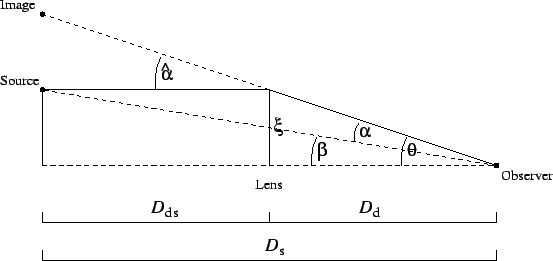
\includegraphics[width=0.7\textwidth]{figures/intro-figures/lens_geometry.png}
	\caption{}
	\label{fig:lens}
\end{figure}

Consider figure \ref{fig:lens}: a ray of light from a source, at a distance $D_s$ from
the observer, deflected due to the lens, at a distance $D_d$ from the observer,  by an 
angle $\hat{\alpha}$ and seen
by the observer at an angle $\theta$ from the lens. If there were no lens, it would have
been observed at $\beta$. Employing small angles approximations, 

\begin{equation}
	\beta  = \theta  - \dfrac{D_{ds}}{D_s} \hat{\alpha}(\xi) \equiv \theta - \alpha(\xi)
	\label{eqn:lens}
\end{equation}
\\
where, $\alpha$ is the scaled deflection angle with respect to the centre of the 
lens to the observed position of the source image and $\xi$ is the impact parameter
of the image on the lens-plane. The equation \ref{eqn:lens} is known
as the {\it lens equation}. The equation describes the true position of the source at $\beta$ to
be seen at $\theta$ due to the lens which is deflecting the light rays by an angle $\alpha$.
If this equation has more than one solution, there will be multiple images of the source. 

For  complex lenses, the 
relation between the deflection angle, $\alpha$, impact parameter, $\xi$ (or $\theta$) and the mass
distribution of the lens can be obtained under the so-called {\it geometrically thin lens}
approximation as,

\begin{equation}
	\alpha(\theta) = \dfrac{1}{\pi} \int d^2\theta^{\prime}
						\kappa(\theta^{\prime})
						\dfrac{\theta-\theta^{\prime}}{|\theta-\theta^{\prime}|^2}
	\label{eqn:alpha}
\end{equation}
\\
where, $\kappa(\theta)$ (or the convergence) is the surface mass density in the 
units of a critical density $\Sigma_{\rm cr}$ defined as,

\begin{equation}
	\kappa(\theta) \equiv \dfrac{\Sigma(\theta)}{\Sigma_{\rm cr}}; 
	\Sigma_{\rm cr} = \dfrac{c^2}{4\pi G} \dfrac{D_s}{D_d D_{ds}}.
\end{equation}

The critical density completely depends on the geometry of the system. For generating
multiple images, $\kappa>1$ and hence the critical density is a characteristic 
surface mass density in order to produce extra images given a source in the background.
Therefore, critical density differentiates between region
of strong and weak lensing, which are described in more details in section \ref{sec:sl}
and \ref{sec:wl}.
\end{comment}


%----------------------------------------------
\subsection{Strong Gravitational Lensing}\label{sec:sl}

Strong gravitational lensing (or SL henceforth), refers to the lensing phenomenon
where the strength of the gravitational field of the lens is sufficiently strong and
the alignment between the source, the lens, and the observer is optimal enough to
produce multiple images of the source. SL regime is marked
by $\kappa >1$ and relatively small values of $\theta$. So, the multiple images of abackground sources contains information about the projected mass distribution of the lens. 

Given the mass distribution of a lens ($\kappa$) and position of the source ($\beta$),
it is straightforward to find out the position of the multiple images ($\theta$), this process
is called {\it forward modelling}. But given a set of multiple images, which are the main 
observables in SL, it is a highly degenerate process to reconstruct the mass
distribution of the lens. The procedure is referred as {\it lens inversion} or
{\it lens modelling} and mainly consist of reconstructing $\kappa$ and
$\beta$ (as in equation \ref{eqn:timedelay}). 

There are 
several methods for lens inversion. Many of those procedures put strong constraints
on the mass distribution of the lens and assume a functional form and hence are called
{\it parametric} methods. These methods mainly involve to find the optimal values 
of the free parameters of the functional form of the mass distribution of the lens. 
For example LENSTOOL\footnote{\url{http://projets.lam.fr/projects/lenstool/wiki}} 
\cite{2011ascl.soft02004K}.

There are some methods which invert the lens with minimal assumptions and without
assuming any prior form of the mass distribution of the lens, and are referred as
{\it non-parametric} methods. In these methods, the number of free parameters are often
too large, usually some building block of the total mass maps, and hence larger
statistical consideration is needed. For example, 
Pixelens\footnote{\url{http://www.physik.uzh.ch/~psaha/lens/pixelens.php}} 
\cite{2011ascl.soft02007S}, 
GRALE\footnote{\url{http://research.edm.uhasselt.be/~jori/page/index.php?n=Physics.Grale}}
\cite{2006MNRAS.367.1209L}.

Where as parametric models are more efficient, non-parametric models are more
accurate and unbiased. In this work we used a non-parametric lens inversion
library called as GRALE \cite{2006MNRAS.367.1209L,2007MNRAS.380.1729L,2009MNRAS.397..341L} 
to trace the mass distribution of some very massive
galaxy clusters. The building blocks of the mass map are the Plummer spheres, where
other choices such as squares and Gaussian spheres are also available in the library, 
and the total mass map is the super position of these building blocks. GRALE uses
a genetic algorithm (for a review see \citep{1995ApJS..101..309C}) 
to find optimal solution to the weights of the building 
blocks and the resolution of the mass maps is adaptively increased (or decreased)
For more detailed documentation see \cite{2009MNRAS.397..341L}.

Another observable in SL is the time delays between multiple images
of the source. The light rays from the same source travel different directions
and due to the curvature of space time, depending upon the mass distribution 
of the lens, they travel different distances before they reach the same 
observer. Because the distances in cosmology depends on the Hubble constant
or the expansion rate of the Universe, one can calculate the value of the
Hubble constant given measured time delays and mass distribution of the source
\cite{2004tomu.conf..231R}. 
However, it is also possible to have the Hubble constant given and put
additional constraints on the mass distribution of the lens using measured
time delays \cite{2015PASJ...67...21M}.


%----------------------------------------------
\subsection{Weak Gravitational Lensing}\label{sec:wl}

Weak gravitational lensing (or WL henceforth) refers to the phenomenon when 
the lensing is not strong enough to produce multiple images but strong enough
to distort the shape of the source. In WL, deformation matrix is close
to unitary matrix.
The deformation of the shape of the observed galaxies
due to the intervening matter is referred to as {\it cosmic shear}. This
signal is very small, nearly 1-2$\%$ of the intrinsic ellipticity of the source 
and can only be measured statistically under the assumption that the intrinsic 
ellipticity of the background galaxies do not have a preferred direction. If one 
measures the cosmic shear of all background sources behind a lens or mass concentration,
it tends to align tangentially towards the centre of the mass concentration. 

As the signal of the weak lensing cosmic shear is very small compared to the 
intrinsic ellipticity of the galaxies, this study did not come into play until
the recent observational and technical advancements. Soon 
after the detection of the giant luminous arc in Abell 370, it was observed
that few more objects that are not as stretched as the giant arc but still show
high axis-ratio and are aligned tangentially towards the centre of the cluster. They
termed it as {\it arclets} and it was clear that the alignment is due to the 
gravitational field of the cluster. It was also expected that there are
only a few very strong distortion of the shapes could happen like the giant 
arc, many more smaller distortions can be observed in the background galaxies.
\cite{1990ApJ...349L...1T} reported the first statistical detection of the WL
cosmic shear in two lensing clusters. The theoretical framework was further
formulated by \cite{1993ApJ...404..441K} and it evolved as an active field
to study the mass distribution of lensing clusters in the outskirts. 

In addition to just studying the local mass concentrations, like galaxies or galaxy
clusters, WL can also be used in order to study the statistical distribution of matter
in an inhomogeneous Universe. Light rays coming from all redshift are continuously
distorted from the matter on its path (figure \ref{fig:wl}). 
For example, light from high redshift sources
are deflected many times as they might witness more mass concentrations in its path, 
as compared to low redshift sources. If the cosmic shear can be measured for 
a large ensemble of sources spread over redshift, the statistical properties
of these shears can be used in order to study the statistical properties of the
cosmological matter distribution and hence infer cosmological parameters. The 
theory and its application was first formulated by \cite{1991MNRAS.251..600B}.
One basic requirement of the underlying theory is to give up the geometrically
thin lens approximation and look at the 3D distribution of matter which 
is then projected onto 2D sky. The theory of weak lensing and its applications
has been reviewed many times, for a thorough review see: \cite{2001stgl.book.....P}.

\begin{figure}
	\centering
	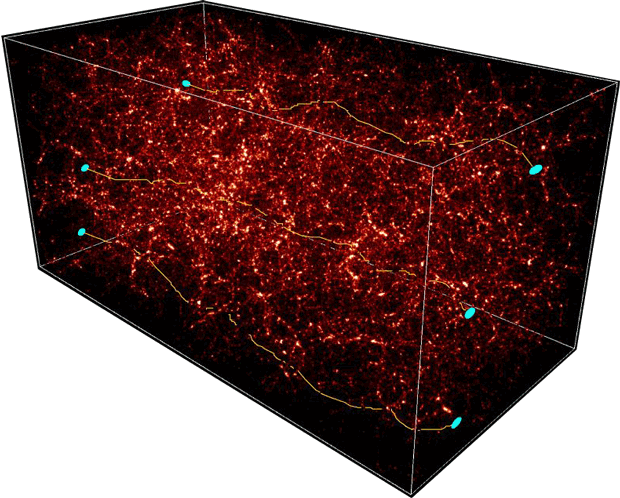
\includegraphics[width=0.7\textwidth]{figures/intro-figures/weaklensing.png}
	\caption{Illustration of weak gravitational lensing by the large-scale
	matter distribution.}
	\label{fig:wl}
\end{figure}

Lets first try to model the statistical properties of the convergence field
$\kappa(\theta)$. In cosmological context, the convergence field can be expressed
as the weighted projection of the mass distribution integrated along the line of 
sight,
\begin{equation}
	\kappa(\theta) = \int_0^{\chi_H} g(\chi)\delta(\chi\theta,\chi) \mathrm{d}\chi
\end{equation}
\\
where, $\delta$ is the 3D relative density contrast as defined in the previous section.
$\chi_H$ is the comoving distance to the horizon and $g(\chi)$ is the lensing 
weight. Under the assumption that largest scale structure in $\delta$ are much smaller
than the effective range $\Delta \chi$ of the projection (also known as the Limber's 
approximation), one can write the lensing weights as,

\begin{equation}
	g(\chi) = \dfrac{3H_0^2\Omega_m}{2c^2} \dfrac{\chi}{a(\chi)\bar{n}} \int_{\chi}^{\chi_(H)}
					n(\chi^{\prime})
					\dfrac{(\chi^{\prime}-\chi)}{\chi^{\prime}}\mathrm{d}\chi^{\prime}
\end{equation}
\\
where, $n(\chi)$ gives the distribution of sources as a function of comoving distance or redshift
and $\bar{n}$ is the number of sources per unit area. These quantities depends on the
experiments like Euclid \cite{2013LRR....16....6A}, LSST \cite{2009arXiv0912.0201L} etc..

As mentioned earlier too, the density field $\delta$ is assumed to be a random field
and only its statistical properties can be modelled, not the individual realisations. 
In the previous chapter, we modelled the second order statistics of this random field
as the matter power spectrum, it is interesting to model similar quantity in lensing,
the power spectrum of the convergence field and relate it to the matter power spectrum.


\begin{equation}
	P_{\kappa}(\ell) \equiv \langle |\tilde{\kappa}|^2 \rangle = 
			\int_0^{\chi_H} \dfrac{g(\chi)^2}{\chi^2} 
			P\left(k=\dfrac{\ell}{\chi},\chi \right) d\chi
\end{equation}
\\
where, $\ell = 180/\theta$, is the multipole and give the angle in the sky. 

If the power spectrum of the convergence field $P_{\kappa}(\ell)$ is observable, it can be
used to constrain the 3D matter power spectrum and hence the cosmological parameters. Further,
the same quantity can also be calculated in different redshift bins (instead of just one) and
auto and cross spectra can be obtained. This process is known as 
lensing {\it tomography} and it has extra constraining power over cosmological parameters
\cite{1999ApJ...522L..21H,2004MNRAS.348..897T}.

Now the last problem is to relate the $P_{\kappa}(\ell)$ to something that is observable, 
possibly the cosmic shear. This is rather direct, as in the complex plane Fourier transform
of the comic shear and that of the
convergence can be related with a phase,
\begin{equation}
	\tilde{\gamma(\ell)} = \exp(2i\beta) \tilde{\kappa(\ell)}
\end{equation}
\\
and therefore we have,
\begin{equation}
	\langle |\tilde{\gamma}(\ell)|^2 \rangle = 
	\langle |\tilde{\kappa}(\ell)|^2 \rangle = P_{\kappa}(\ell)
\end{equation}
\\
i.e., the power spectrum of the cosmic shear is the same as the cosmic shear of the
convergence field. Therefore, cosmic shear can be measured in a wide survey and the 
power spectrum is calculated which can be used in order to put constraints on
cosmology.


%----------------------------------------------

%------------------------------------------------------------------------------
%------------------------------------------------------------------------------

\section{Motivation}

The theory of structure formation is partially understood --  at large scales 
or during early dark ages when the perturbations are tiny or only linear order is important. 
However, for small scale clustering processes, when the higher order in perturbations 
become important, the analytic solutions are not possible, and we rely on simulations and 
approximations. Also, as baryons play a vital role at small scale clustering
and galaxy formation, it is also important to quantify these effects and 
understand various baryonic processes. 
The main motivation of this work is to model the distribution of matter in high dense
regions like lensing clusters and in the large scale structures of the Universe. 
This information is useful in two ways: 

First, the accurate modelling of the matter distribution in individual clusters
give information about the properties of dark-matter. On large scales, dark-matter
is known to be collision-less and non-interacting except for its gravitational effects,
but it is important to quantify and test the hypothesis in high density regions, like
at the centre of clusters. A small but finite cross section of dark-matter particles
can be well tested in high density regions, this may have stronger implications for our 
understanding of the properties of dark-matter and the Universe at large.  
Also, as the baryonic processes and theory of galaxy
formation is poorly understood, the central regions of the galaxy clusters can be 
used as laboratories to study these processes. It can be done only if the matter 
distribution in the individual systems is well constrained. 
Further, following the hierarchical structure formation, many small halos interacts and
merge to form large collapsed virialised structures; the study of the distribution of 
matter in lensing clusters at high redshift give information about the merging
stage of the cluster. 

Modelling of the distribution of matter in the large scale structures of the  
Universe is very important
in order to model the cosmological observables. Statistically, the modelling of the
matter power spectrum or 2PCF is important if one wants to do cosmology because 
the matter power spectrum underlies many
cosmological observables like Baryon Acoustic Oscillations (BAO), 
weak lensing, galaxy clustering, redshift
space distortions etc.. Also, the modelling of the 
covariance matrix of the matter power spectrum is vital in order to do correct
likelihood analysis and testing cosmological models. Finally baryonic physics 
also changes the power spectrum at small scales, if neglected, it will add biases
in the cosmological parameters and mislead the interpretations. 

\subsection{Challenges}

There are certain challenges in order to accurately model the mass distribution
in clusters and in the Universe. 

\begin{itemize}
	\item Distribution of matter in clusters: Mass is not an observable, what we 
			observe is the light in different frequency bands. We can derive 
			redshift, velocity dispersions etc. from this. To relate these observables
			to mass distributions, we have approximations and various models which
			are often rich in systematics, i.e., the incomplete understanding and 
			biases. Gravitational lensing is far the most unbiased technique in order
			to trace matter in lenses. However, even in lensing the inversion of the lens
			is a highly degenerate process. Often and very much in 
			practice, people assume that mass follows light, which is a good approximation
			but may not be true everywhere. So, this is essential that the 
			mass reconstruction techniques are independent of such assumptions in order
			to learn about intrinsic properties of the dark-matter and baryonic
			process in the high dense regions of the lensing clusters.

	\item Modelling matter power spectrum and its covariance matrix: In order to model
			the matter power spectrum at non-linear scales, simulations are by far the 
			best solution as all other analytic approaches are difficult. But this is limited
			by the volume and resolution of the simulation. Also a good simulation
			can be very expensive computationally. So, it is possible to simulate a big
			volume at very good resolution for a cosmological realization, but in order
			to carry out a likelihood analysis on some cosmological data, simulations are
			very expensive and often impossible to do. So, we rely on semi-analytic models, 
			which can model the matter power spectrum with some function of cosmology
			and are more accurate than the perturbation theories etc. at non-linear 
			scales. Similarly, in order to get good covariance matrix of the matter power
			spectrum from simulation, we need to simulate a volume of the order 
			1000 $(h^{-1} \mathrm{Gpc})^3$
			cube, which again is very expensive specially when small scale modelling 
			is necessary. 

	\item Modelling baryonic physics in two-point functions: Finally baryonic effects are 
			important at small scales statistically. If these effects are not present
			in the model of the power spectrum, it will bias the whole exercise and
			the recovered cosmology might be very precise but not accurate. 
\end{itemize}

The main goal of this work is to target these challenges. 
I performed and completed
a number of projects in order to achieve these goals,
As a result, I successfully completed five scientific papers
that are attached with this manuscript.


%==============================================================================
% Chapter 2: Paper 1
%==============================================================================

\chapter{Mass--Galaxy Offsets in Lensing Clusters}
\label{chap:mass-galaxy-offsets}

\section{Introduction to the Paper}

In the concordance model of cosmology, cold dark matter (CDM) provides the major
budget for the matter content in the Universe, nearly 80$\%$. 
It interacts only gravitationally and provides a large potential well that
attracts low mass halos to form high mass halos
through a series of mergers. Baryons follow these potential wells
and cool down to form stars and galaxies. Therefore, it is safe to assume
that light-follows-mass in these giant halos. However, there could be a number of
astrophysical and/or cosmological scenarios where light-follows-mass does not hold. 
For example, if the dark matter interacts with baryons or with itself. This
kind of non-standard properties of the dark-matter can be tested in 
dense regions like the centre of the galaxy clusters. Strong gravitational lensing is 
an ideal tool to obtain this information as it is sensitive to the total
mass of the lens, and does not differentiate between dark-matter or luminous
galaxies.

In this paper, we studied the mass-galaxy offsets in three lensing clusters of galaxies:
Abell 3827, Abell 2218 and Abell 1689. These three clusters are very different in 
their morphology, total mass, redshift, and lensing data. We used GRALE, a strong
gravitational lens inversion library, to model the mass maps of these clusters given
the position of the multiple images of the background sources 
and their redshift. No information
from the lensing clusters was used, except for their redshift. The
mass models are completely form free. We also provide the uncertainty
maps that show high-confidence in the region where lensing images were present. 

Because of the free-form and high certainties of the mass maps, 
it is possible to compare the distribution
of matter in these clusters with luminous galaxies
completely on the basis of statistical uncertainties. In Abell 3827 and
Abell 2218 we found small offsets between the local mass peaks and the
position of a nearby galaxy. Particularly, in Abell 3827 this offset is nearly 6 kpc,
and is statistically significant. We also discussed the possible origin 
of these offsets, which can be either astrophysical like dynamical
friction or the non-standard properties of the dark-matter component like
self-interactions. 
The offset in Abell 3827 is further studied by Massey et al. 2015 with new HST
data where the offset was found to be robust. With a simplified model, we argued that
to explain this offset, the cross-section of dark-matter particles 
$\sigma/m$ must be of the order $10^{-4}$.

In Abell 1689, no significant offsets were found. However,  
we found a line of sight sub-structure behind the cluster at
redshift $\sim 3$. 

\paragraph{Role:} Under the supervision of Dr. Prasenjit Saha,
I started this project by modifying some parts of 
GRALE library for an optimised fitness function, and resolution scheme
using two simulated cluster lenses: (i) a simple circular lens, and 
(ii) a lens with similar morphology as that of Abell 3827. I proposed the
idea of reconstructing three clusters, two of which are known for
mass-galaxy offsets in previous studies, 
and a third one without it. The motivation was to set examples 
of clusters having large offsets, small offsets, and no offset, which we
found in Abell 3827, Abell 2218 and Abell 1689 respectively. I accumulated
the lensing data for the three clusters, and reconstructed their mass 
maps using GRALE. In Abell 3827, I quantified the offsets statistically
by locating the centre of mass in a circle around the galaxy closest to 
the local sub-peak. I also proposed the idea to find a line of sight
substructure, if any, by using sources in bins of redshift.


This paper has been published in {\it Monthly Notices of the Royal Astronomical
Society} (MNRAS). 
\\
Arxiv: \url{http://arxiv.org/abs/1402.4217}


\begin{publishedpaper}
  {\fontsize{18}{22}\selectfont\scshape
   Mass--Galaxy Offsets in Abell 3827, 2218 and 1689:\par
   Intrinsic Properties or Line-of-Sight Substructures?\par}

  \vspace{1.25em}

  {\large
   Irshad Mohammed, Jori Liesenborgs,\par
   Prasenjit Saha, and Liliya L.~R. Williams\par}

  \vspace{1.25em}
  {\small
   Published in \textit{Monthly Notices of the Royal Astronomical Society}\par
   \url{https://arxiv.org/abs/1402.4217}\par}
\end{publishedpaper}

\begin{paperabstract}
We have made mass maps of three strong-lensing clusters, Abell 3827,
Abell 2218 and Abell 1689, in order to test for mass-light offsets.
The technique used is GRALE, which enables lens reconstruction with
minimal assumptions, and specifically with no information about the cluster
light being given.  In the first two of these clusters, we find local
mass peaks in the central regions that are displaced from the nearby
galaxies by a few to several kpc.  These offsets {\em could\/} be due
to line of sight structure unrelated to the clusters, but that is very
unlikely, given the typical levels of chance line-of-sight
coincidences in $\Lambda CDM$ simulations --- for Abell 3827 and Abell
2218 the offsets appear to be intrinsic.  In the case of Abell 1689,
we see no significant offsets in the central region, but we do detect
a possible line of sight structure: it appears only when sources at
$z\ga 3$ are used for reconstructing the mass.  We discuss possible
origins of the mass-galaxy offsets in Abell 3827 and Abell 2218: these
include pure gravitational effects like dynamical friction, but also
non-standard mechanisms like self-interacting dark-matter.
\end{paperabstract}


\vspace{1em}
\noindent \textbf{Keywords:} gravitational lensing: strong, galaxies: clusters: individual: Abell 1689, Abell 2218, Abell 3827
\vspace{1em}


% \begin{multicols}{2}

%%%%%%%%%%%%%%%%%%%%%%%%%%%%%%%%%%%%%%%%%%%%%%%%%%%%%%%%%%%%%%%%%%%%%%%%%%
\section{Introduction}

Our current understanding of the universe and its dynamics indicates
that its major components are dark: cold dark-matter (CDM) and the
so-called ``dark-energy''.  Unlike baryons, dark-matter
interacts only gravitationally and provides the deep potential wells
which are followed by the baryons. The baryons form clumps at these
potential wells and cool down to form stars.  The standard
$\Lambda$CDM model explains a range of observed processes pretty well,
from the angular power spectrum of the cosmic microwave background \citep{2013arXiv1303.5075P} to
the baryonic acoustic oscillations \citep{2013MNRAS.433.1202S} in the large scale structure and
the number counts of clusters.  However, the intrinsic properties and
behaviour of dark-matter and dark-energy remain an open problem in
cosmology.

In the picture of hierarchical structure formation in $\Lambda$CDM
model, galaxy-clusters are the most recently formed structures that
are gravitationally bound. They are cosmic laboratories to test
the laws of gravity, structure formations and the interaction of
different species of particles. A galaxy cluster contains lots of
galaxies --- tens to thousands, hot intra-cluster plasma visible in
X-rays, a variety of of relativistic particles and finally dark-matter
which dominates its mass budget.  Measuring the mass of the galaxy-cluster 
is an essential aspect of using the cluster to study many other things.
There are several physical processes that enable one to measure
the mass: the kinematics of cluster galaxies
\citep{2013ApJ...772...47S}, the hydrodynamics of hot gas emitting
X-rays \citep{2009ApJ...692.1033V}, and gravitational lensing.  Lensing
is particular interesting, because it relies only on gravity and does
not itself require any luminous objects in the cluster being studied.
One of the questions that lensing can address is how well the luminous matter
traces the distribution of total mass. Deviations, or lack thereof, from the
mass-follows-light hypothesis will provide important information about the 
physical processes going in within clusters. The first lensing-based detection 
of deviations from mass-follows-light goes back to the late 1990's 
\citep{1998AJ....116.1541A} but the observation that generated a wide interest 
in these deviations was that of the Bullet Cluster \citep{2006ApJ...648L.109C}, 
which showed unambiguously that dark matter is quite collisionless compared to 
the gas phase baryonic matter \citep{2008ApJ...679.1173R}. While the properties 
of dark matter are probably not the only reason for deviations from mass-follows-light
in galaxy clusters, dark matter self-interaction cross-section and how to optimally
extract it from observations is an exciting avenue of research 
\citep{2013arXiv1310.1731H,2013MNRAS.433.1517H}.

This work uses strong gravitational lensing to look for deviations from 
mass-follows-light, i.e. it explores the correspondence on the sky between the
dark-matter peaks with the galaxies in the central parts of three
galaxy clusters, Abell 3827, 2218 and 1689. These clusters are very
different from each other in morphology and redshift. 
%A manifestation about nature/properties of dark-matter is also proposed.
As we discuss in Section~\ref{sec:p1-discussion}, some deviations we find may be due to the 
non-standard properties of dark matter, but others could be the result of 
superimposed substructure, or hydrodynamics within the cluster. 

We use GRALE \citep{2006MNRAS.367.1209L,2007MNRAS.380.1729L}, a
strong-gravitational lensing tool to reconstruct the mass map of the
clusters.  There is no overall parametric form for the mass
distribution, but rather an adaptive grid.  Other than the redshift,
no information about the cluster is required as input, not even its
location or morphology.  This makes GRALE well-suited to reconstruction of
mass maps before comparison with light.



%%%%%%%%%%%%%%%%%%%%%%%%%%%%%%%%%%%%%%%%%%%%%%%%%%%%%%%%%%%%%%%%%%%%%%%%%%


\section{The lens-reconstruction technique}

GRALE has been applied to other strong-lensing clusters
\citep{2008MNRAS.389..415L,2009MNRAS.397..341L}
and compared with other techniques
\citep{2010MNRAS.408.1916Z,2011MNRAS.413.1753Z}, so here we just give
a general description and then some tests.

\subsection{Grale}

The data given to GRALE consist of the identified multiple-image
systems and their redshifts, along with possible regions where
additional images are guessed to be likely.  No information about the
light from the lens is given.  The mass maps in GRALE are free-form,
being made up of a superposition of many components.  In the present
work, each component is taken as a Plummer lens, that is, the usual
Plummer sphere
\begin{equation}
\rho = \frac{3M}{4\pi} \frac{a^2}{(r^2+a^2)^{5/2}}
\end{equation}
projected to two dimensions.  Other choices of lens component, such
as square tiles, are also possible.

Any mass distribution in GRALE is assigned a fitness with respect to the
given data.  The fitness has two components, as follows.

\begin{enumerate}
\item For a given mass map, the input images are ray-traced back to
  the source, using the lens equation.  The more nearly these
  back-projected images coincide for any multiple-image system, the
  fitter the mass map.  If the fitness measure were simply the
  source-plane distance between the back-projected images, that would
  favour extreme magnification (tiny sources); accordingly, the fitnes
  measure is scaled to the source size.
\item There could be further places in the image plane that, when
  ray-traced back to the source, coincide with the sources
  corresponding to the observed images.  These correspond to extra
  images, and would be favoured by the above fitness measure.  There
  may indeed be undiscovered extra images in certain regions, but in
  most of the image plane, extra images can be ruled out with high
  confidence.  The area of no images present is referred to in GRALE
  as the null space.  For each image system, the user specifies a null
  space, which is simply the image plane with the images themselves
  cut out, and (optionally) further cutouts where incipient images
  could potentially be present.  Images in the null space lead to a
  fitness penalty for the mass map.
\end{enumerate}

It is possible to have other components to the fitness, such as time
delays for quasar source \citep{2009MNRAS.397..341L}, but the present
work uses these two.  The null space, item (ii) above, is a unique
aspect of GRALE.  There are other techniques that allow the mass
distribution to be very general in form, as with GRALE, but they make
additional assumptions in order to suppress extra images, such as constraining
local density gradients \citep{2006ApJ...652L...5S} or applying smooth
interpolation schemes \cite{2008ApJ...681..814C}.  Only GRALE
incorporates the absence of images as useful data.

The computational part of GRALE is optimizing the fitness function for
the given data, using a genetic algorithm.  The basic idea, inspired
by Darwinian evolution, is to generate a population of trial
solutions. A fitness measure is assigned to each trial solution and
then these solutions are combined, cloned and mutated to get the next
generation of populations supported by a better fitness function.
Genetic algorithms have long been used in astrophysics for hard
optimization problems \citep[for a somewhat old but readable review,
  see][]{1995ApJS..101..309C}.  They tend to be computationally
expensive, but are often effective on otherwise intractable problems.
GRALE uses a multi-objective genetic algorithm, meaning that the
different components of the fitness function are compared
individually, not just combined into a single function.  Only the
fitness ranking matters in genetic algorithms, not the actual values
of the fitness.  In terms of likelihoods and posterior probabilities,
models with better fitness are considered more probable, that is, the
fitness components are monotonic in the posterior probability, but
there is no known or assumed functional relation between likelihood
and fitness.

The locations and masses of the Plummer components are chosen by the
genetic algorithm.  The algorithm also adapts the number of Plummers,
but an allowed range is specified by the user.  That is, the user
specifies the level of substructure.  For the GRALE fitness measure,
lower is better, and it decreases as we increase the resolution of the
map.  This is quite intuitive as more Plummer spheres naturally result
in a better fit.  So the overall criterion should be somehow a
function of the GRALE fitness measure and the number of Plummers.  We
are not aware of any theoretical argument that yields the appropriate
criterion, but after some experimentation we found one that works
reasonably well in test cases.  This is an `unfitness' or
\begin{equation} \label{eq:p1-badness}
\hbox{badness} = \ln\left(\hbox{GRALE fitness} \times
                     \sqrt{\hbox{number of components}}\,\right) .
\end{equation}
If we think of the GRALE fitness measure as a mismatch distance, and
the number of Plummers as the inverse resolution length, the badness
criterion appears natural.

To choose the number of Plummer components, we adopted the following
procedure.  First, we have GRALE reconstruct the lens with a
comparatively low number of Plummers.  Then we let GRALE improve the
fit with progressively more Plummers, allowing more substructure to be
introduced.  After that, we let GRALE continue to adapt the fit with
progressively fewer Plummers.  The mass distribution with the minimum
badness \eqref{eq:p1-badness} is taken as the result.

%%%%%%%%%%%%%%%%%%%%%%%%%%%%%%%%%%%%%%%%%%%%%%%%%%%%%%%%%%%%%%%%%%%%%%%%%%


We now report on two simulated lenses, which we generated and then
reconstructed with GRALE, in order to check the pipeline and calibrate
the error estimates.  

\subsection{A simple lens}

A Plummer lens of mass $10^{14} $M$_\odot$ was generated at redshift
0.1.  Six sources were put at different redshifts (one at 0.15, two
at 0.2, two at 0.4 and one at 1.0).  The mass profile and image plane
are shown in Figure \ref{fig:p1-plummer-input}.  The images and source
redshifts were given to the inversion module of GRALE.
Figure~\ref{fig:p1-plummer-output} shows the reconstructed masses at
different resolutions and the badness values.

When reconstructing the lens, GRALE did not have the information that
in fact it had a simple parametric form, without substructures.  The
reconstructions do have some substructure, as well as small offsets
from the centre.  Such spurious features increase with resolution.
The least-badness criterion, however, favours a model with relatively
little substructure.

\begin{figure}[p]
  \centering
  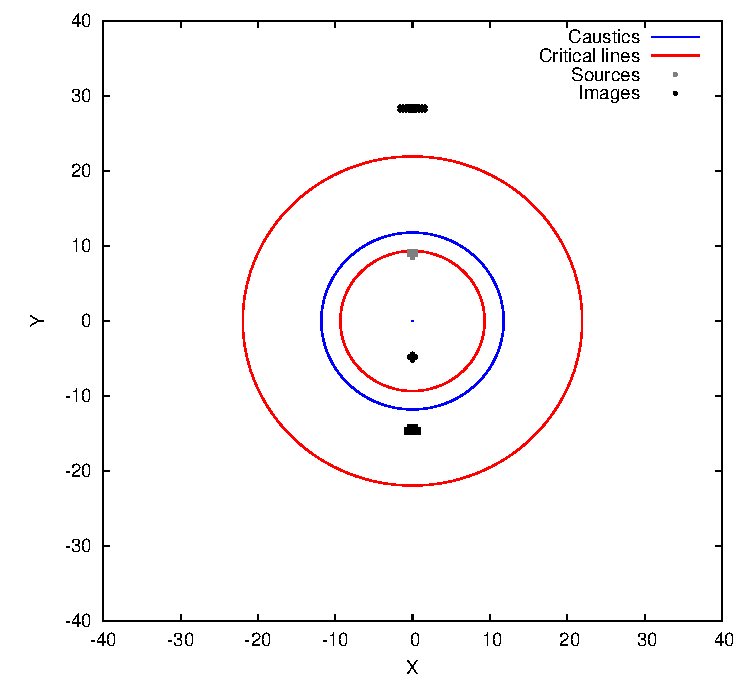
\includegraphics[width=0.24\linewidth]{figures/p1-figures/imgplane5plummer.pdf}
  \hfil
  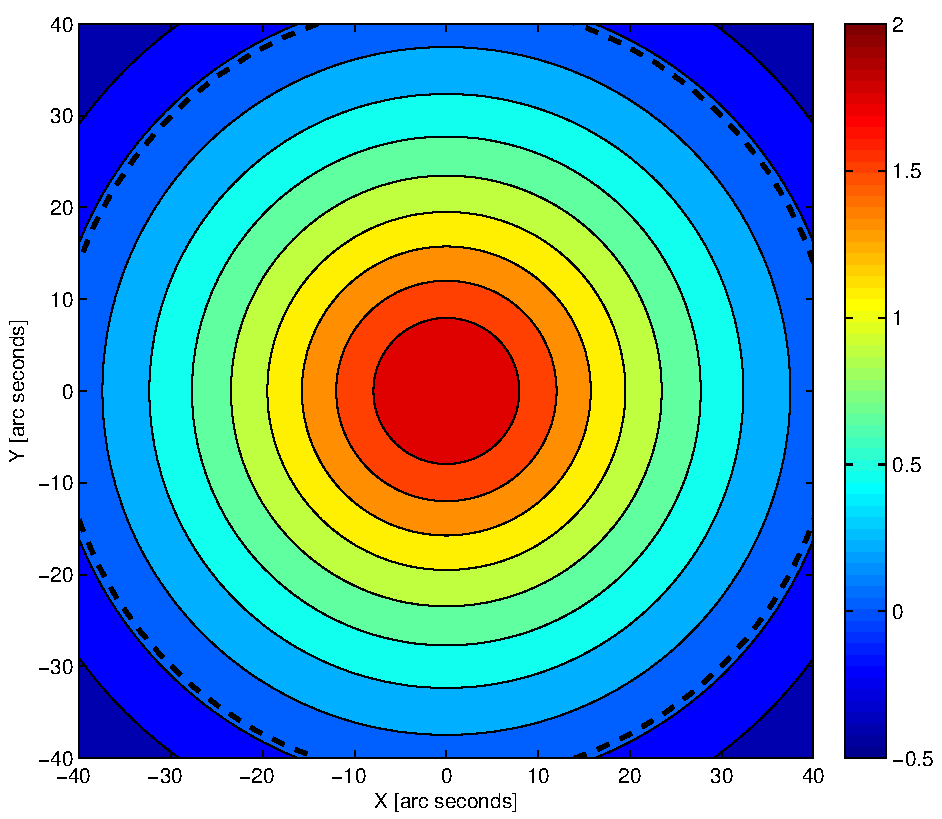
\includegraphics[width=0.3\linewidth]{figures/p1-figures/lensplummer.pdf}
  \hfil
  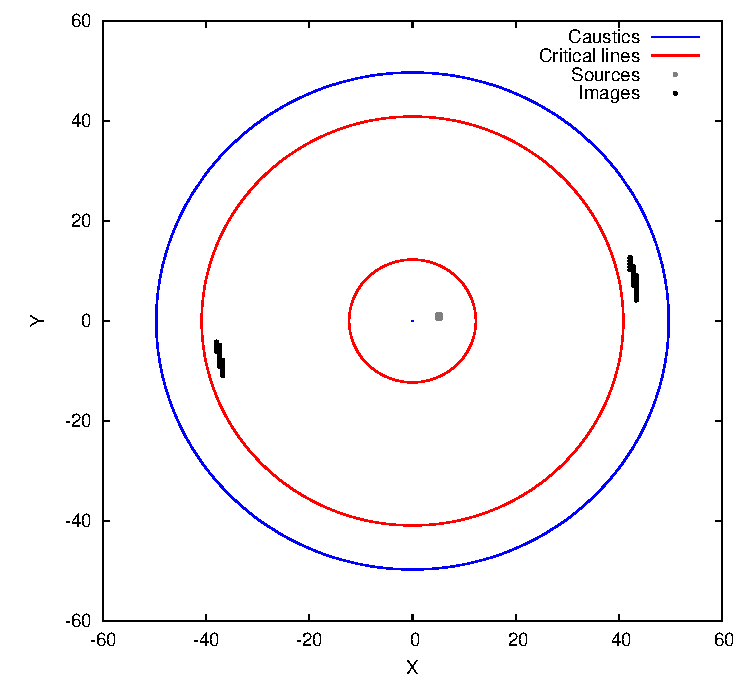
\includegraphics[width=0.24\linewidth]{figures/p1-figures/imgplane6plummer.pdf}\\
  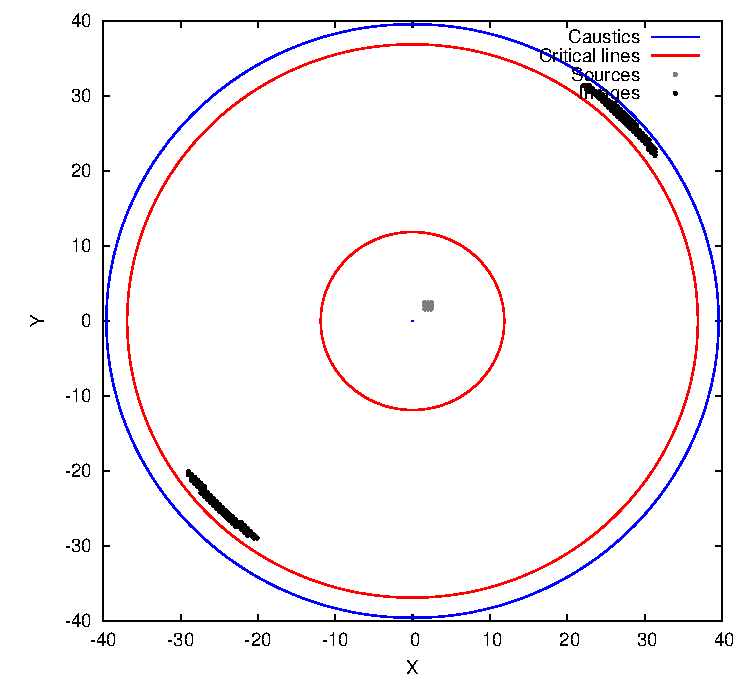
\includegraphics[width=0.24\linewidth]{figures/p1-figures/imgplane3plummer.pdf}
  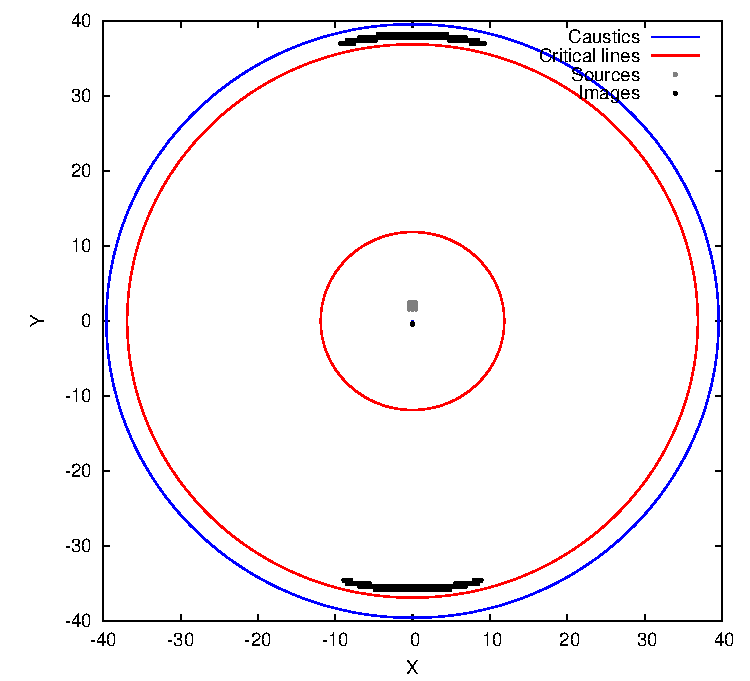
\includegraphics[width=0.24\linewidth]{figures/p1-figures/imgplane4plummer.pdf}
  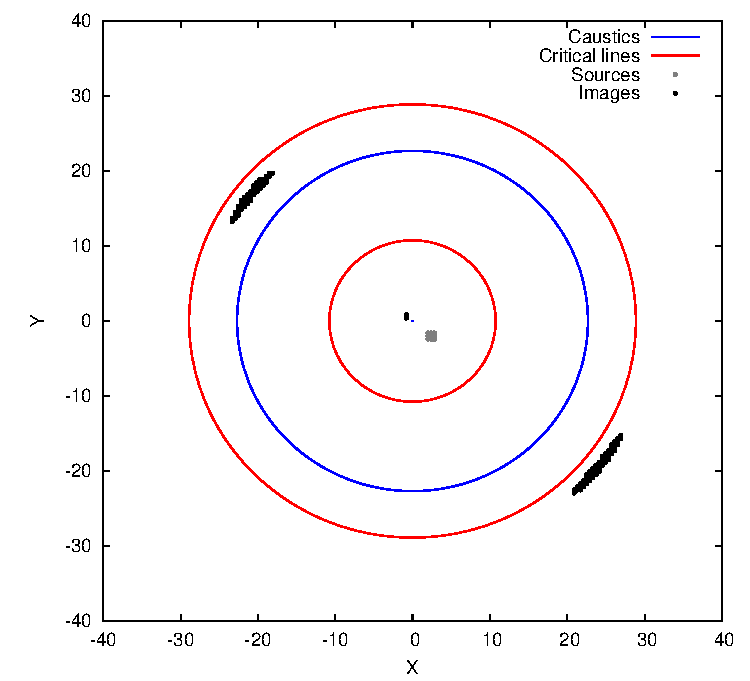
\includegraphics[width=0.24\linewidth]{figures/p1-figures/imgplane1plummer.pdf}
  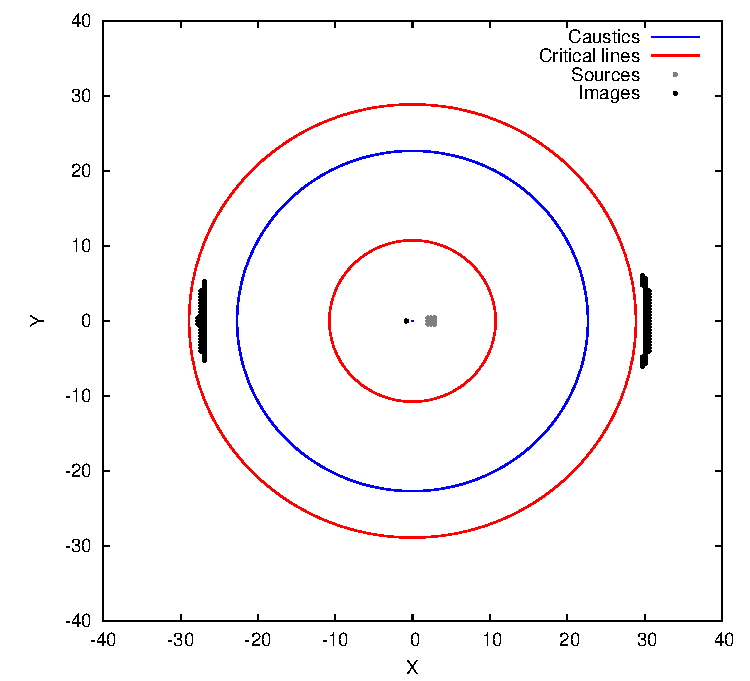
\includegraphics[width=0.24\linewidth]{figures/p1-figures/imgplane2plummer.pdf}
\caption{\label{fig:p1-plummer-input} A circularly symmetric synthetic lens
  (centre top panel) and six image systems from sources at different
  redshifts. Sources are in grey, caustics are in blue, critical
  curves are in red. The contour lines in the synthetic lens are those
  of constant surface mass density; the color scale is in units of
  log~(kg~m$^{-2}$). The same scale is used in all figures in this
  paper. For reference, $\Sigma_{\rm crit}$ for $z_l=0.1$ and $z_s=0.2$
  in a standard $\Lambda$CDM cosmology is $18.7$ kg~m$^{-2}$.}
\end{figure}

\begin{figure}[p]
  \centering
  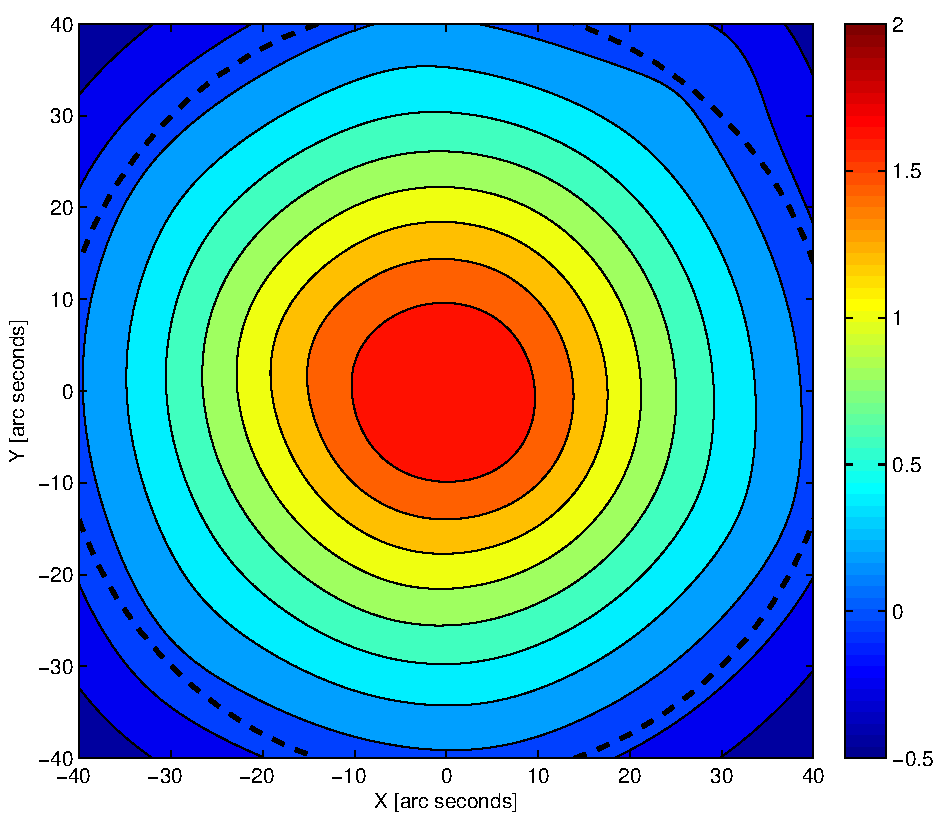
\includegraphics[width=0.3\linewidth]{figures/p1-figures/lens1plummer.pdf}
  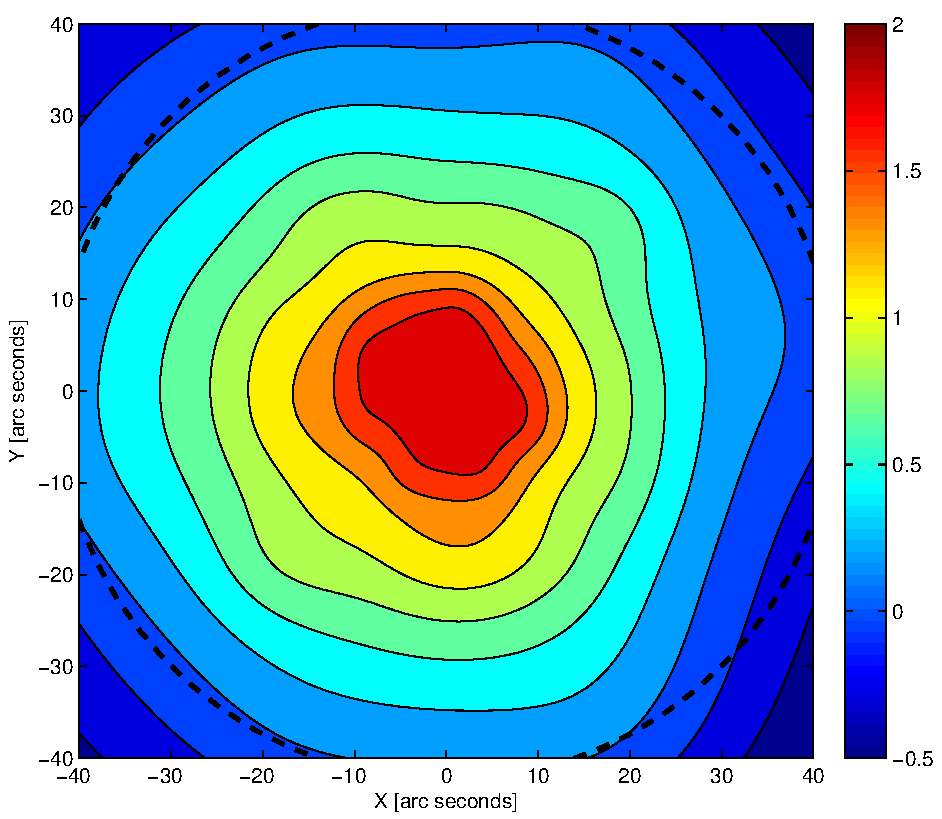
\includegraphics[width=0.3\linewidth]{figures/p1-figures/lens2plummer.pdf} 
  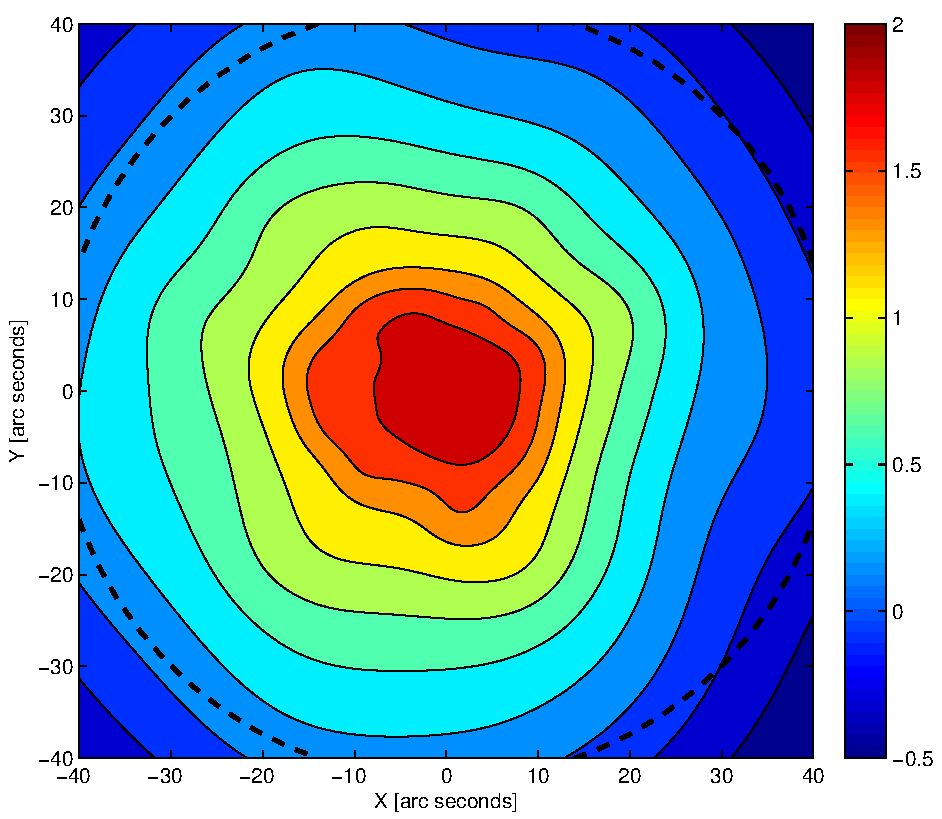
\includegraphics[width=0.3\linewidth]{figures/p1-figures/lens3plummer.pdf}\\
  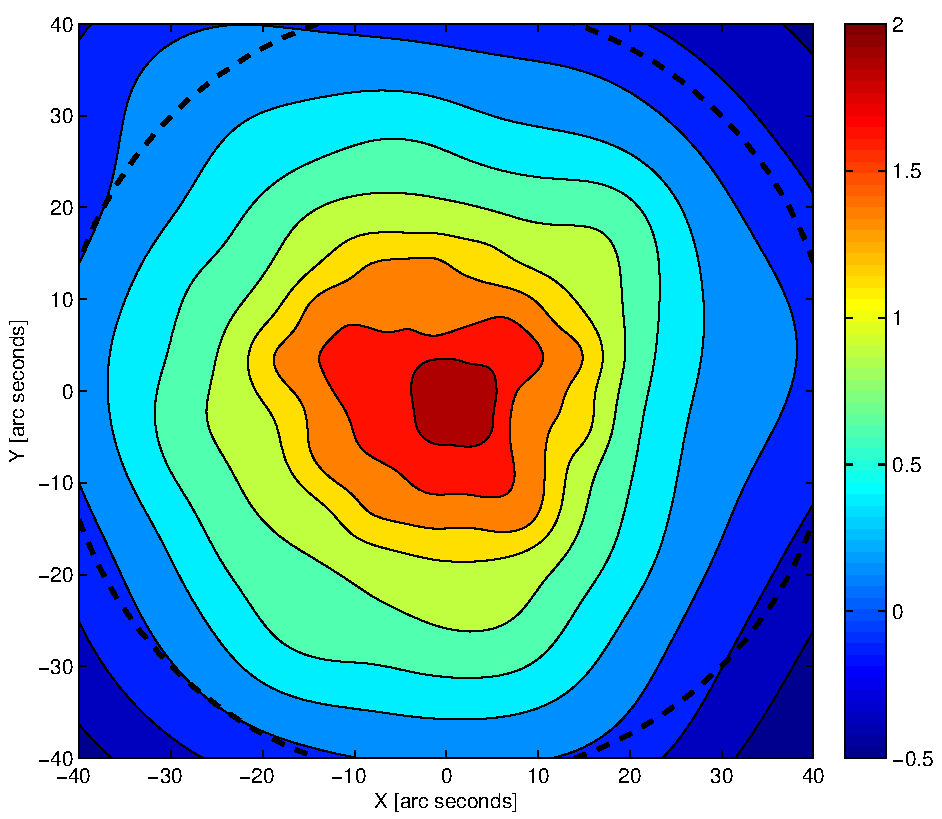
\includegraphics[width=0.3\linewidth]{figures/p1-figures/lens4plummer.pdf} 
  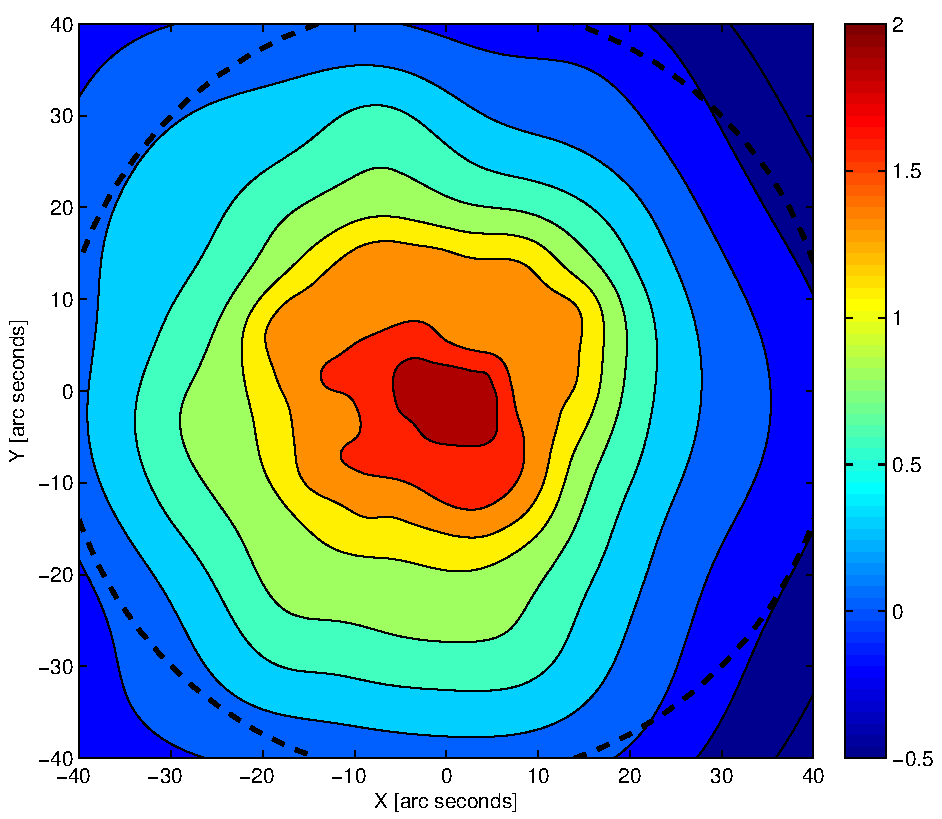
\includegraphics[width=0.3\linewidth]{figures/p1-figures/lens5plummer.pdf}
  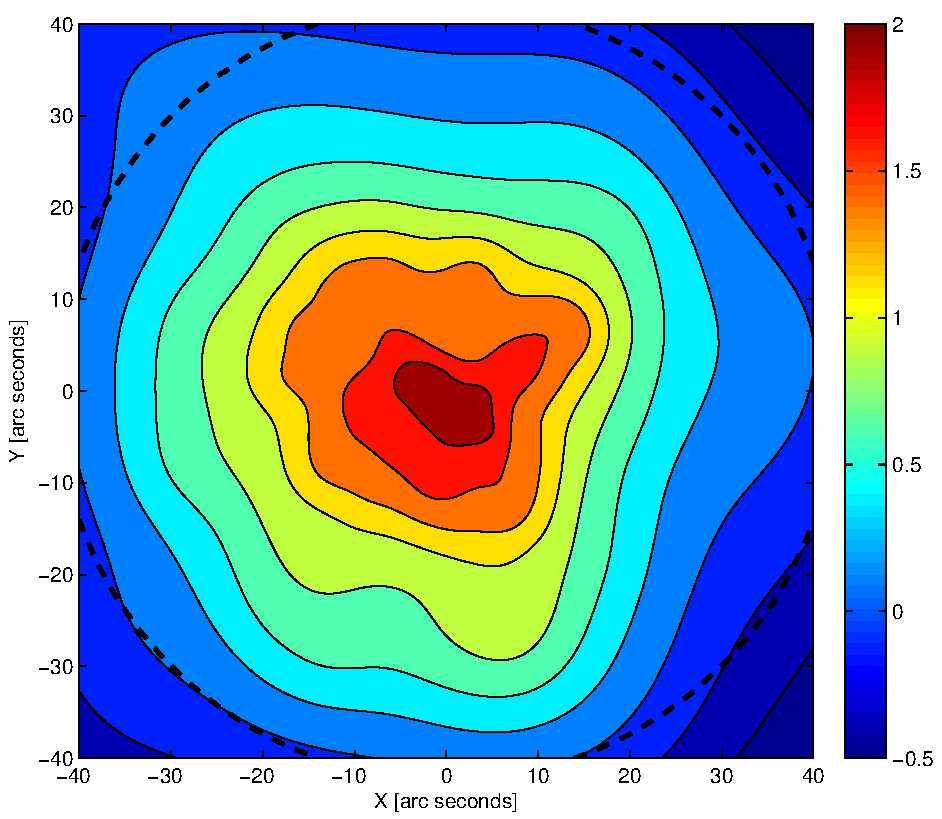
\includegraphics[width=0.3\linewidth]{figures/p1-figures/lens6plummer.pdf}\\
  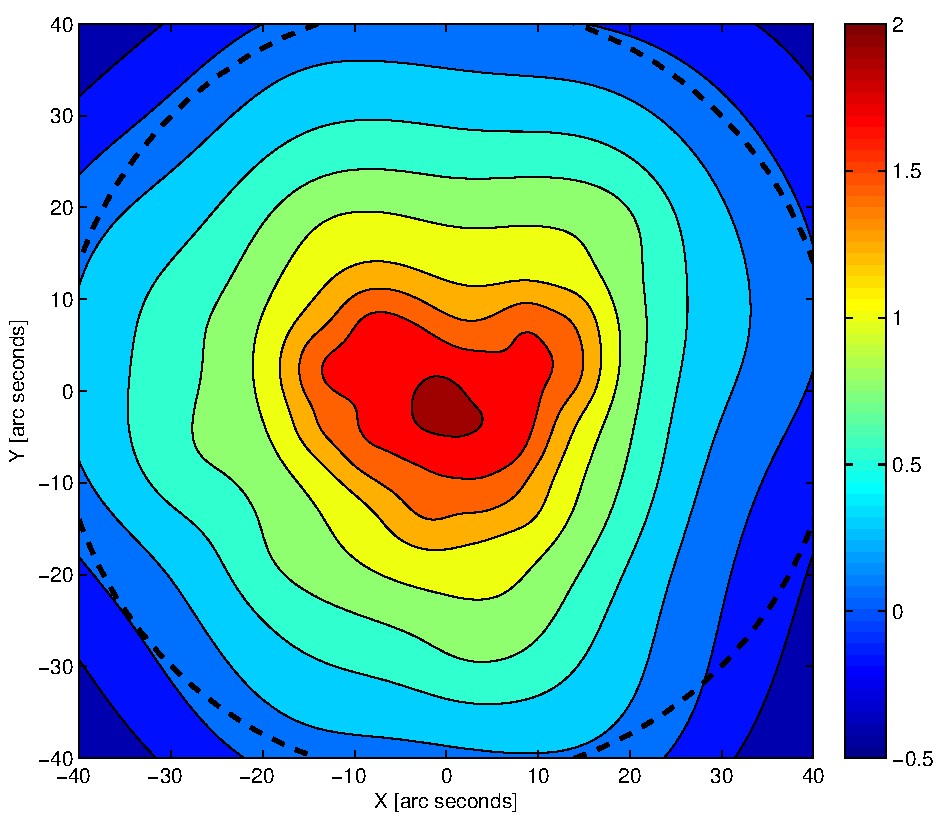
\includegraphics[width=0.3\linewidth]{figures/p1-figures/lens7plummer.pdf}
  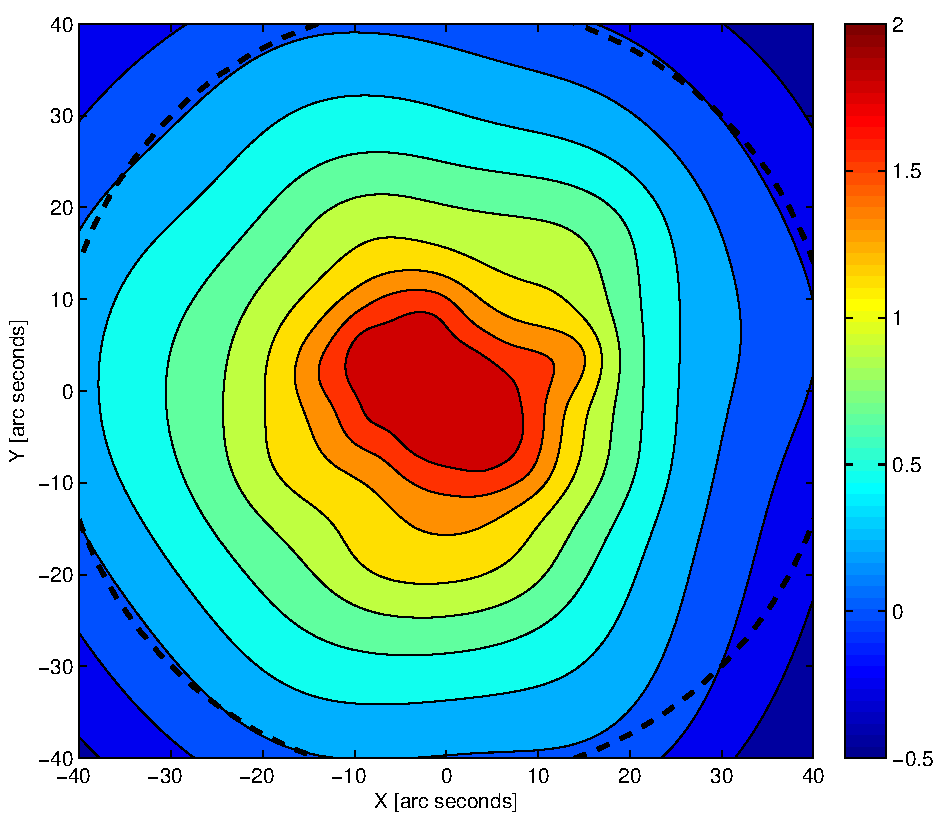
\includegraphics[width=0.3\linewidth]{figures/p1-figures/lens8plummer.pdf} 
  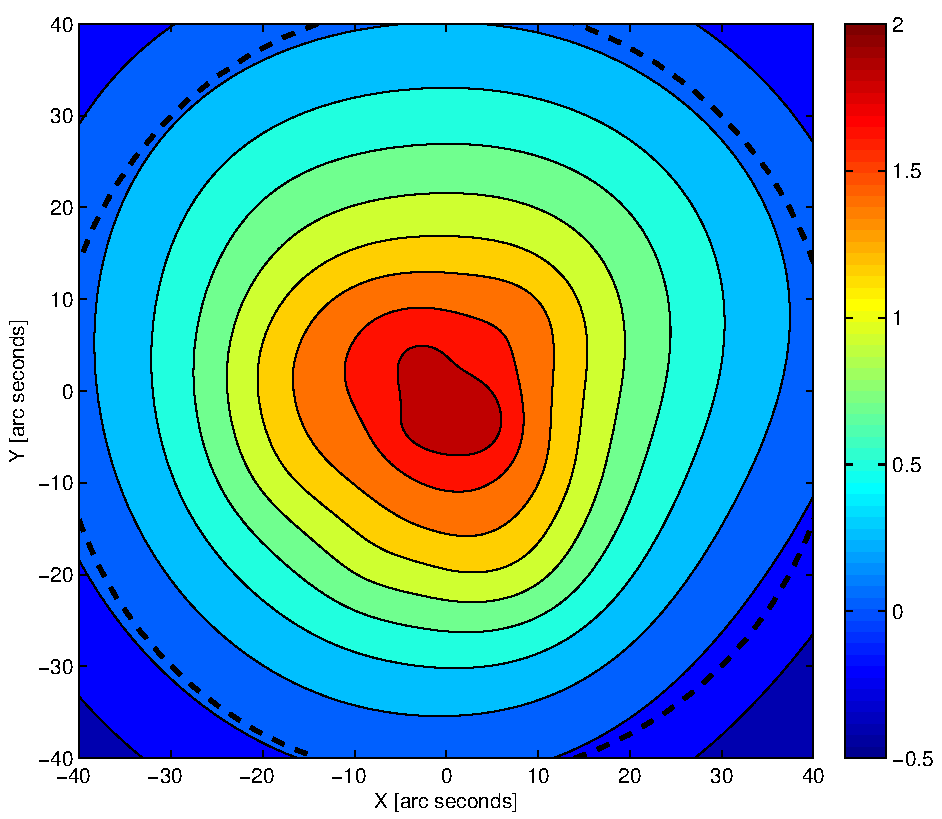
\includegraphics[width=0.3\linewidth]{figures/p1-figures/lens9plummer.pdf}\\
  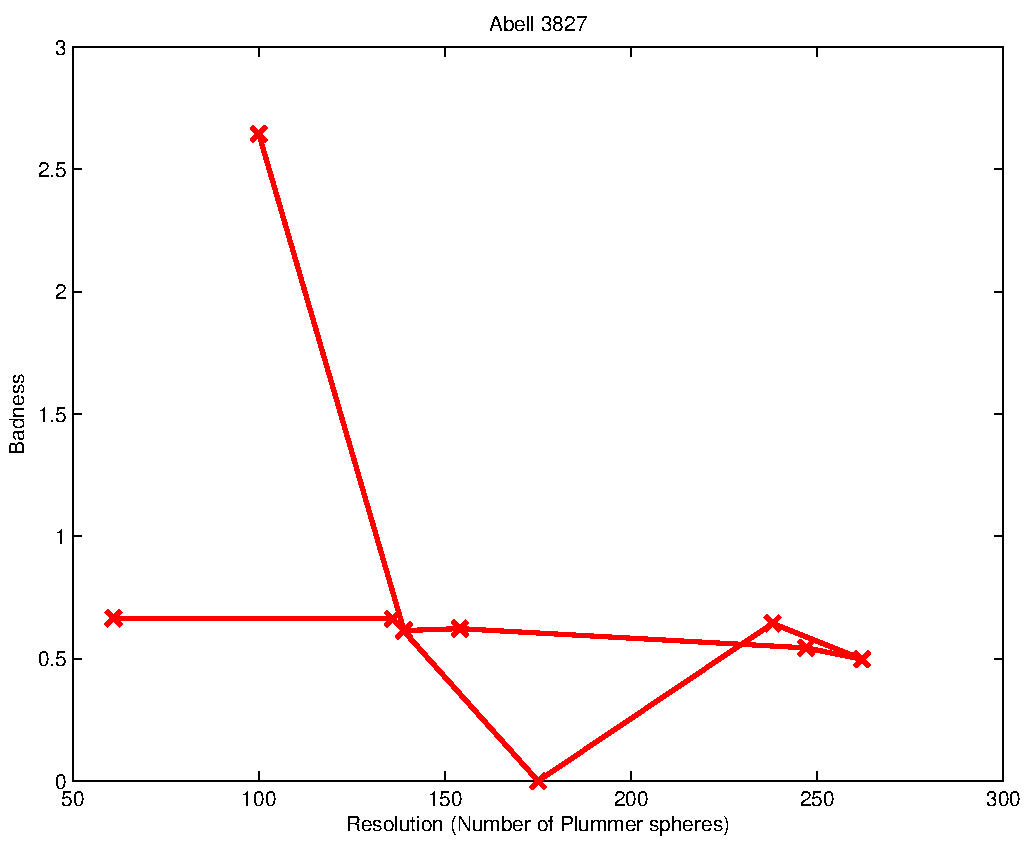
\includegraphics[width=0.4\linewidth]{figures/p1-figures/fitness_simulationplummer.pdf}

\caption{Reconstruction of the lens in
  Figure~\ref{fig:p1-plummer-input} from the data in that figure.  The
  badness curve (bottom panel) shows that the best
  model is the third one (top right map in the grid of nine.) The dashed
  circle in each map delineates the modeled region. \label{fig:p1-plummer-output}.
The sequence of mass maps is in reading order (from top-left to bottom-right).}
\end{figure}

\clearpage

\subsection{A more complex lens}

We now increase the complexity, both of the input lens and of the
reconstruction procedure.  For each data set, from now on we will
present a mean map $\Sigma$ and a fraction rms-deviation map
$\delta\Sigma/\Sigma$, obtained as follows.  From the images, we first
let GRALE construct a sequence of maps at nine different resolutions
(as with the simple lens), and then select the one at minimum badness.
This whole procedure is repeated 10 times, to obtain an ensemble of
reconstructions.  The mean and rms deviation refer to such an
ensemble, as
\begin{equation}
\delta\Sigma = \left(\langle\Sigma^2\rangle - 
                     \langle\Sigma\rangle^2\right)^{\frac12} \,.
\end{equation}
Each map of $\Sigma$ and $\delta\Sigma/\Sigma$ comes out of 90 separate
reconstructions at different resolutions.  The typical computational
requirement is 50~hours $\times$ 16 cores.

A simulated lens at redshift 0.1 was next created with five Plummers
positioned such that the configuration resembles the inner region of
Abell 3827.  Sources were put at different redshifts, as
follows.
\begin{enumerate}
\item Three-source case: three sources at $z=0.2$ were were given as input.
\item Four-source case: a fourth source at $z=0.4$ was added.
\item Five-source cases: a fifth source at $z=1.0$ was added.
\end{enumerate}
The resulting images, along with caustics and critical curves, is
shown in Figure \ref{fig:p1-complex-input}).  Results from these are shown
in Figure \ref{fig:p1-complex-output}.  The top row of the figure shows the
mass maps $\Sigma$.  The second row shows $\delta\Sigma/\Sigma$, or
the fractional rms deviation.  The third row shows
$\Delta\Sigma/\delta\Sigma$ where $\Delta\Sigma$ is the (absolute)
actual deviation of the reconstructed mass map from the real mass map.  
If $\delta\Sigma$ were close to $\Delta\Sigma$, we
could simply take the rms deviation as the uncertainty.  In fact the
rms deviation under-estimates the true error by about a factor of two.
That can be read off the bottom row of Figure \ref{fig:p1-complex-output},
which plots the cumulative distribution of
$\Delta\Sigma/\delta\Sigma$.

The main result from this test is that the rms deviation times two is
a reasonable approximation of the errors.  In addition, we can also read off some
qualitative features from Figure \ref{fig:p1-complex-output}. First, the
spur or handle-like feature to the lower right is recovered in the
lens reconstruction in all cases, even if not perfectly reproduced.
Second, the maps get more accurate as more sources, especially at
different redshifts, are introduced.

We conclude that GRALE is able to find offsets as well as extended
structures (if any) in lenses.

%%%%%%%%%%%%%%%%%%%%%%%%%%%%%%%%%%%%%%%%%%%%%%%%%%%%%%%%%%%%%%%%%%%%%%%%%%

\begin{figure}[p]
  \centering
  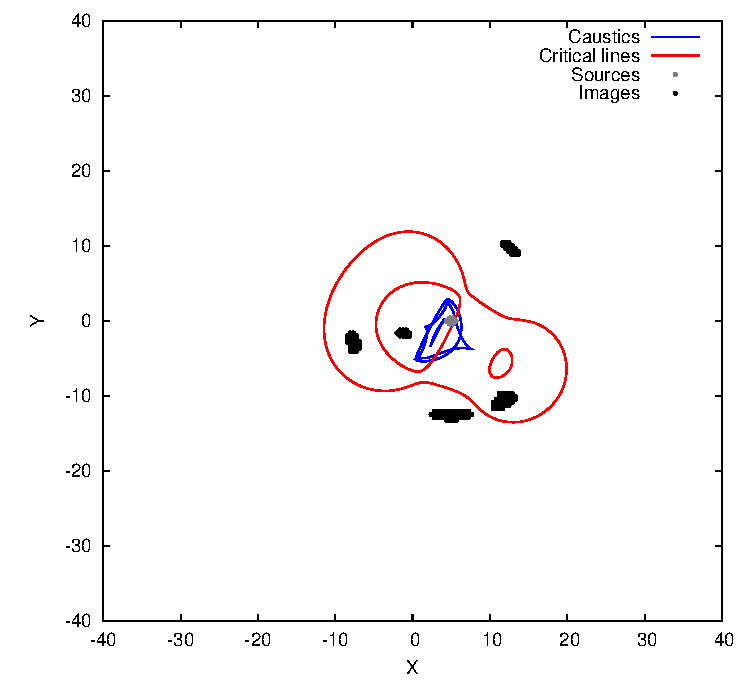
\includegraphics[width=0.24\linewidth]{figures/p1-figures/imgplane4plummer5.pdf}
  \hfil
  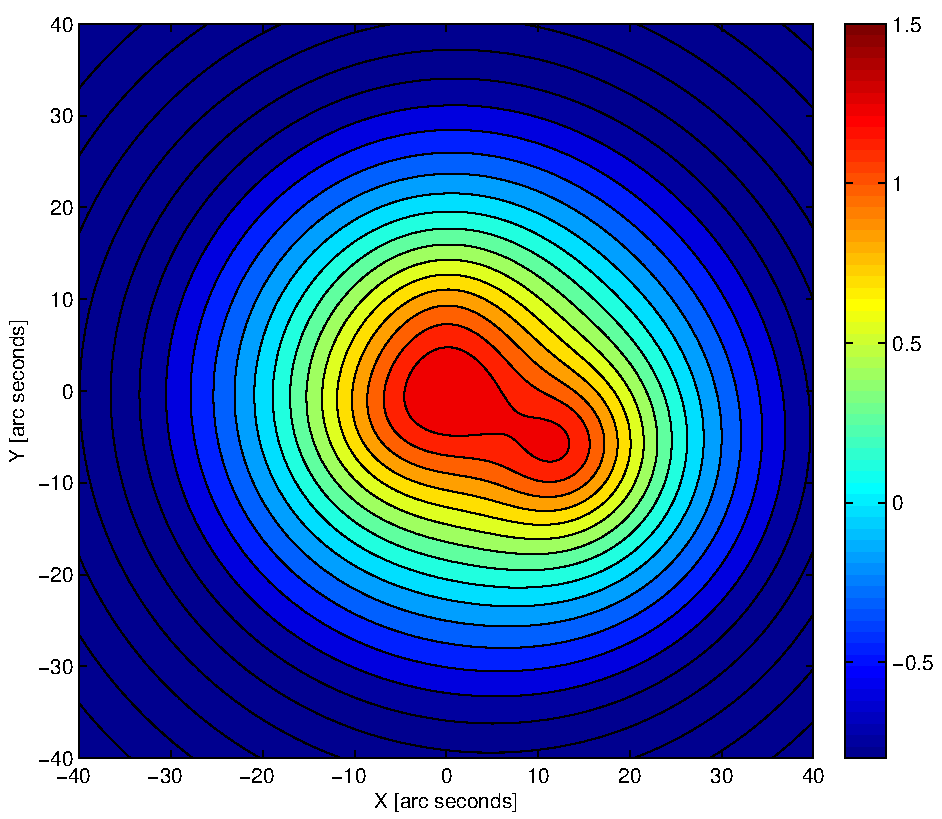
\includegraphics[width=0.3\linewidth]{figures/p1-figures/lensplummer5.pdf}
  \hfil
  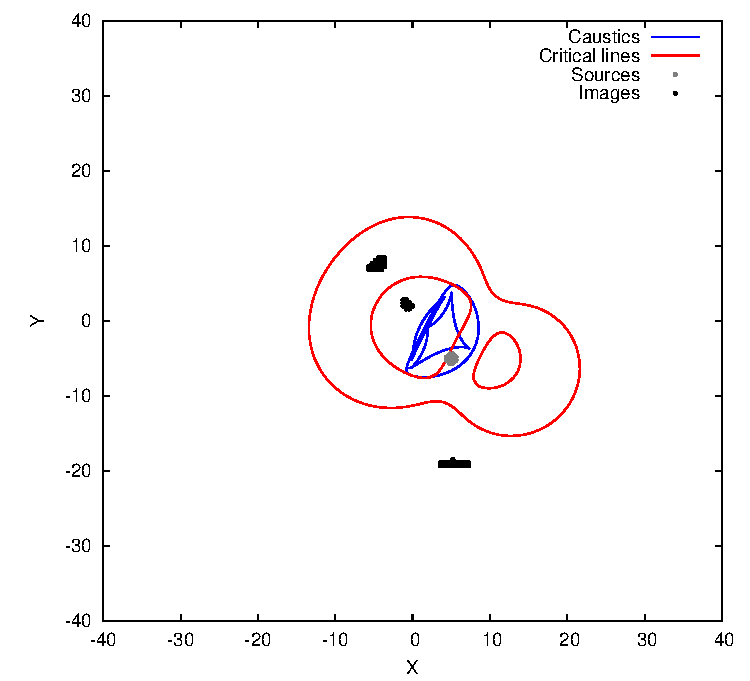
\includegraphics[width=0.24\linewidth]{figures/p1-figures/imgplane5plummer5.pdf}\\
  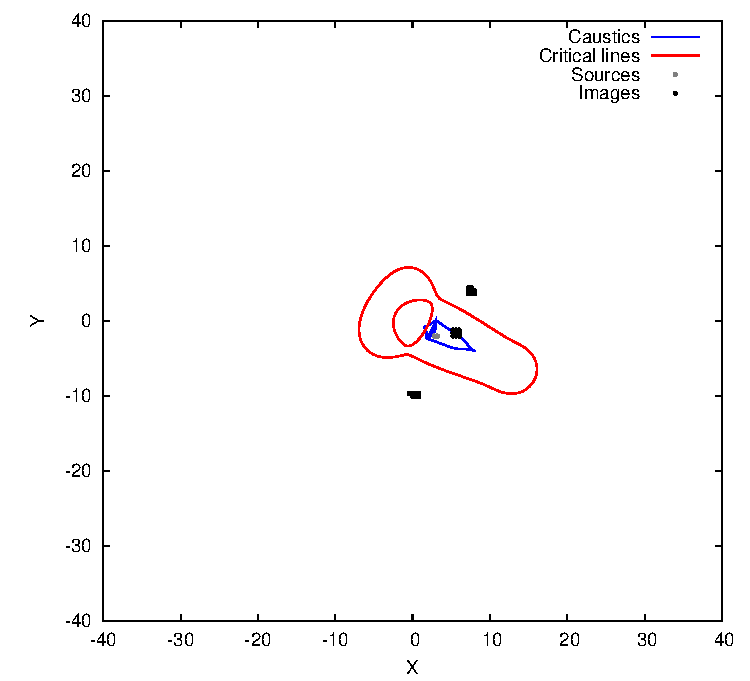
\includegraphics[width=0.24\linewidth]{figures/p1-figures/imgplane1plummer5.pdf}
  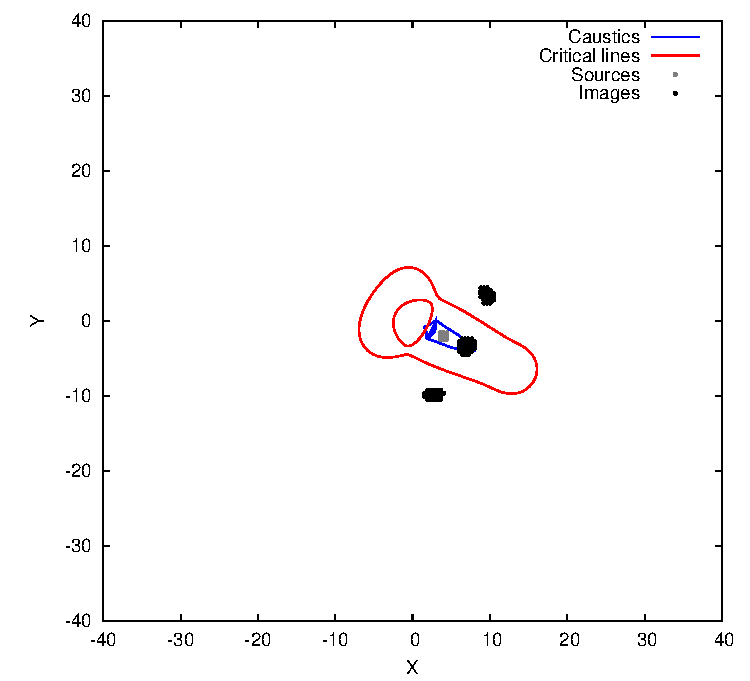
\includegraphics[width=0.24\linewidth]{figures/p1-figures/imgplane2plummer5.pdf}
  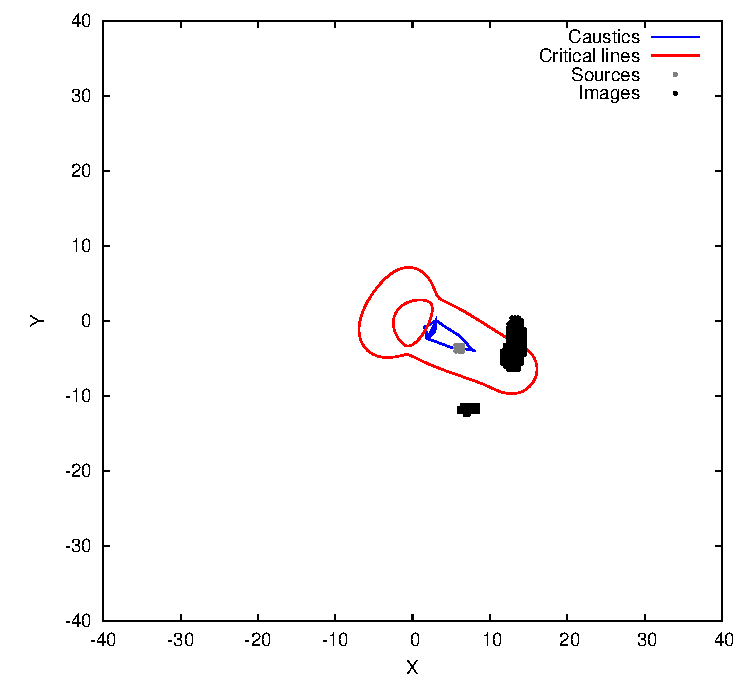
\includegraphics[width=0.24\linewidth]{figures/p1-figures/imgplane3plummer5.pdf}
\caption{\label{fig:p1-complex-input} A synthetic lens with a main
  mass concentration and a nearby secondary mass peak. Five projected Plummer
  spheres are used to construct this lens. Image systems from five
  sources at different redshifts are shown in separate panels.}
\end{figure}

\begin{figure}[p]
  \centering
  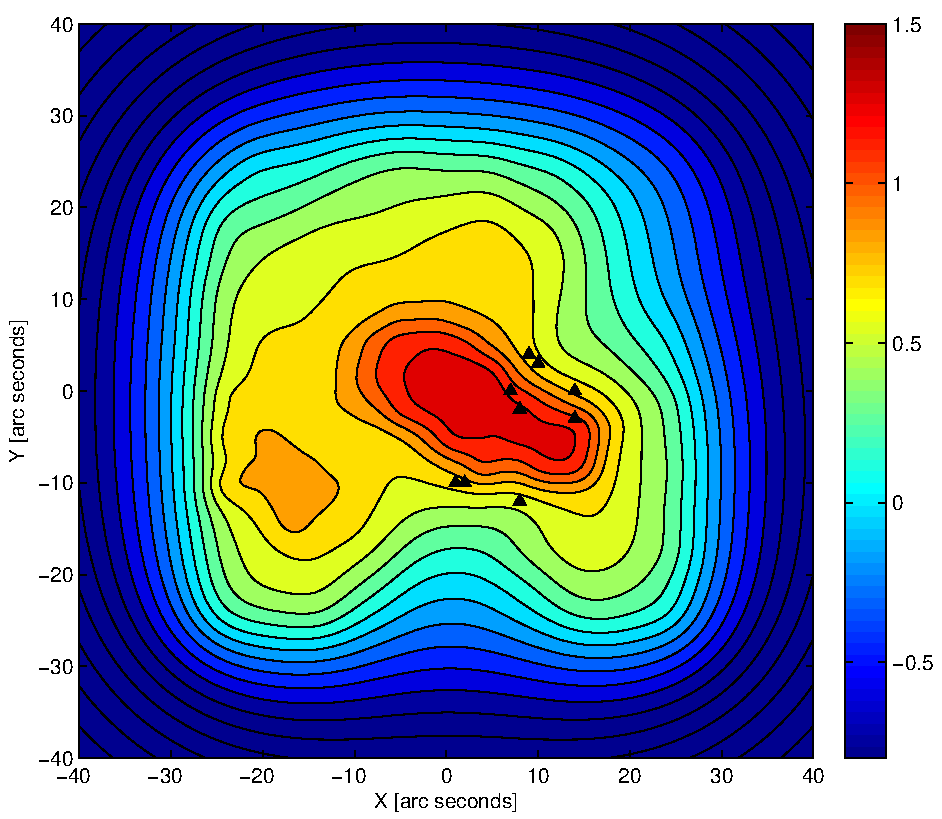
\includegraphics[width=0.32\linewidth]{figures/p1-figures/average3sources5plummer.pdf}
  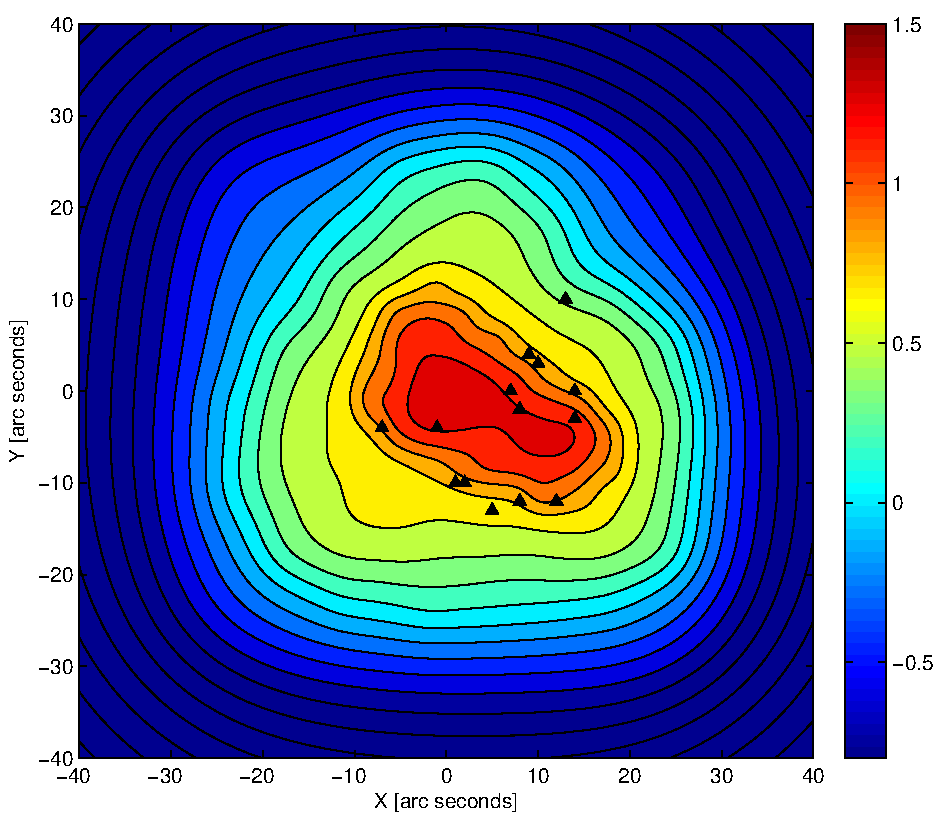
\includegraphics[width=0.32\linewidth]{figures/p1-figures/average4sources5plummer.pdf}
  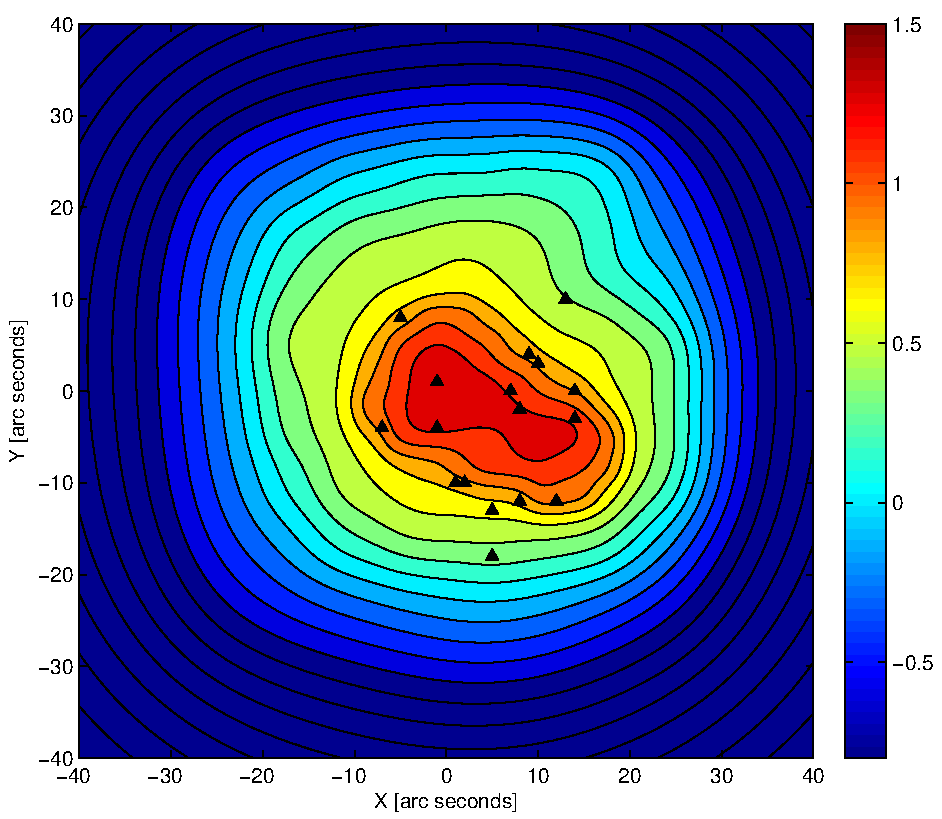
\includegraphics[width=0.32\linewidth]{figures/p1-figures/average5sources5plummer.pdf}\\

  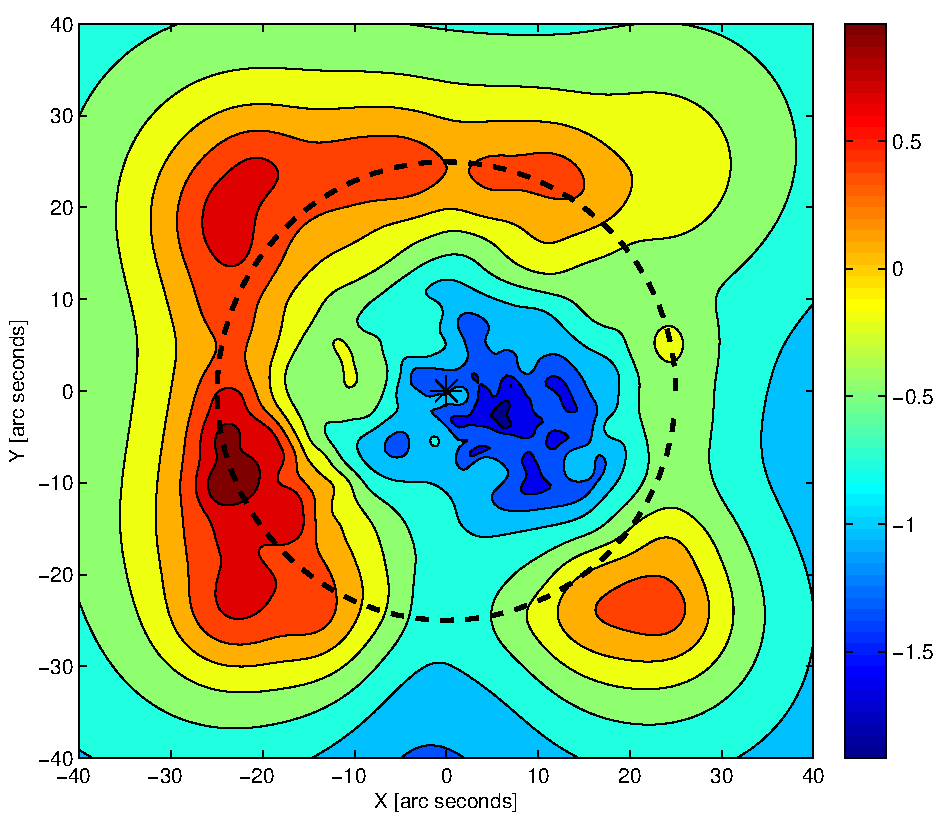
\includegraphics[width=0.32\linewidth]{figures/p1-figures/error13sources5plummer.pdf}
  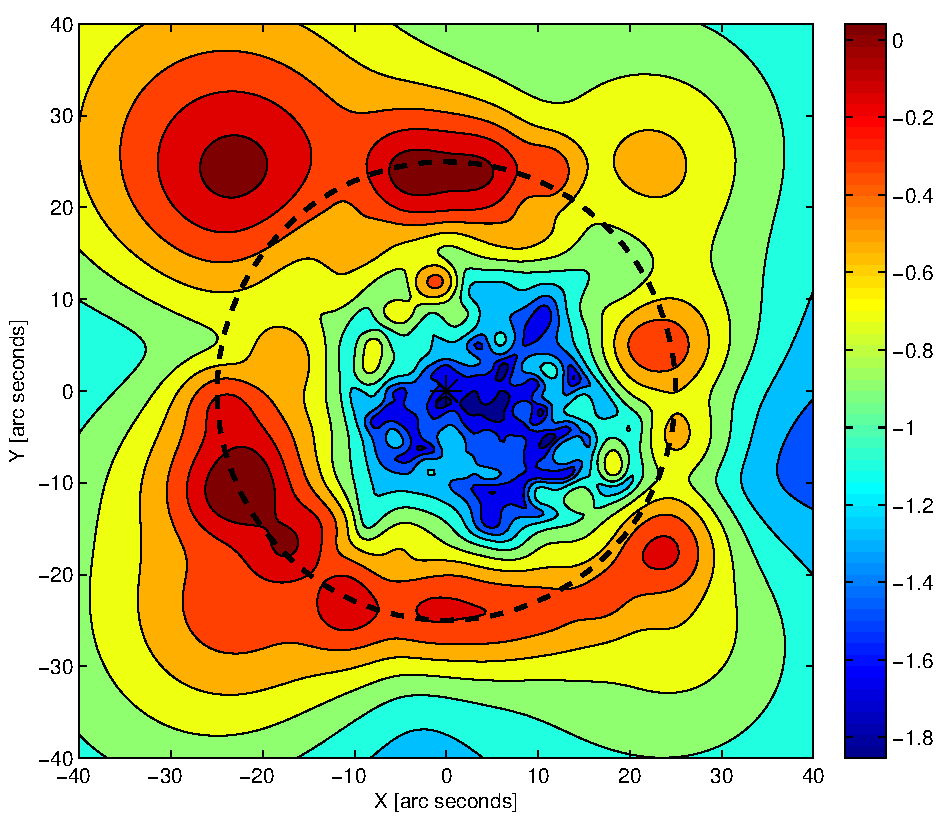
\includegraphics[width=0.32\linewidth]{figures/p1-figures/error14sources5plummer.pdf}
  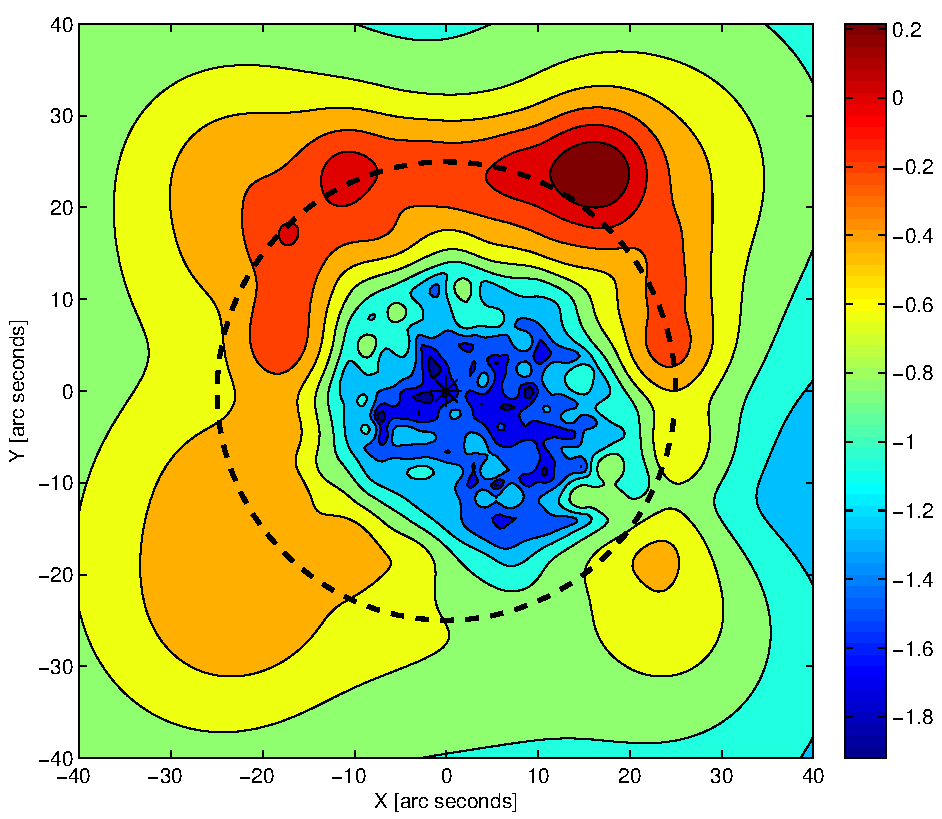
\includegraphics[width=0.32\linewidth]{figures/p1-figures/error15sources5plummer.pdf}\\

  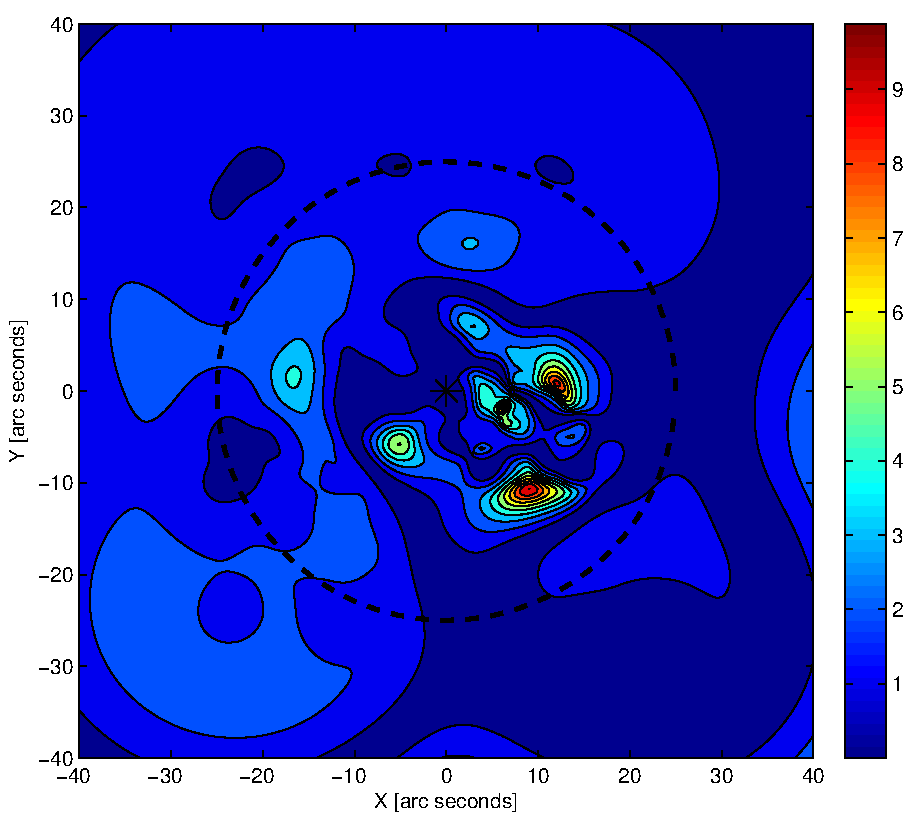
\includegraphics[width=0.32\linewidth]{figures/p1-figures/error23sources5plummer.pdf}
  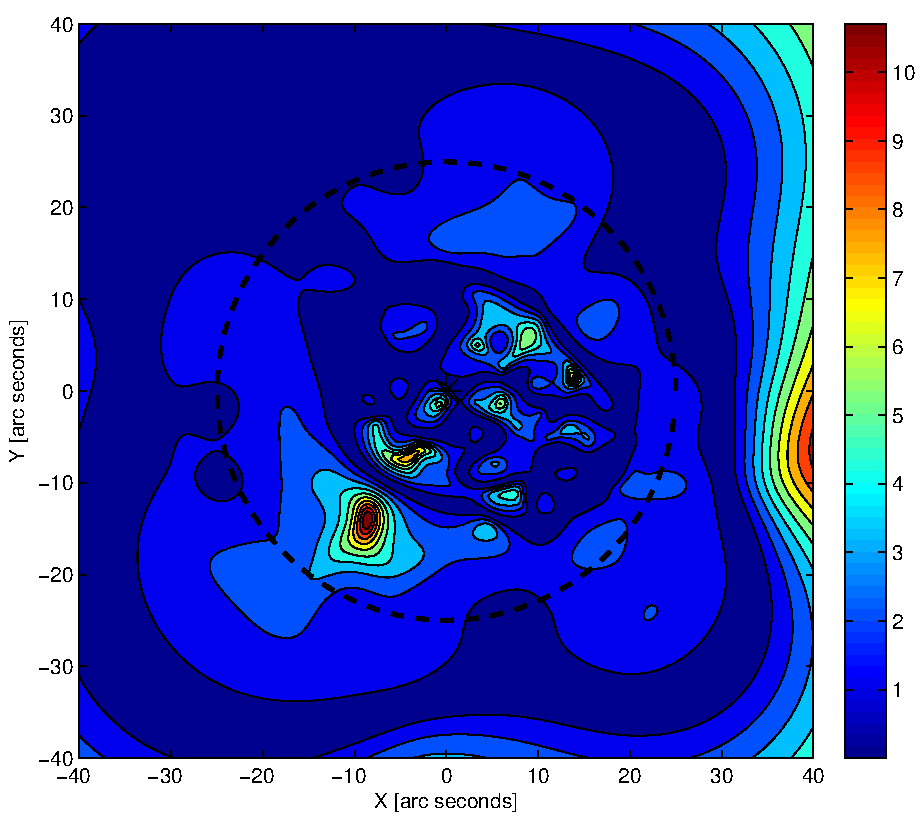
\includegraphics[width=0.32\linewidth]{figures/p1-figures/error24sources5plummer.pdf}
  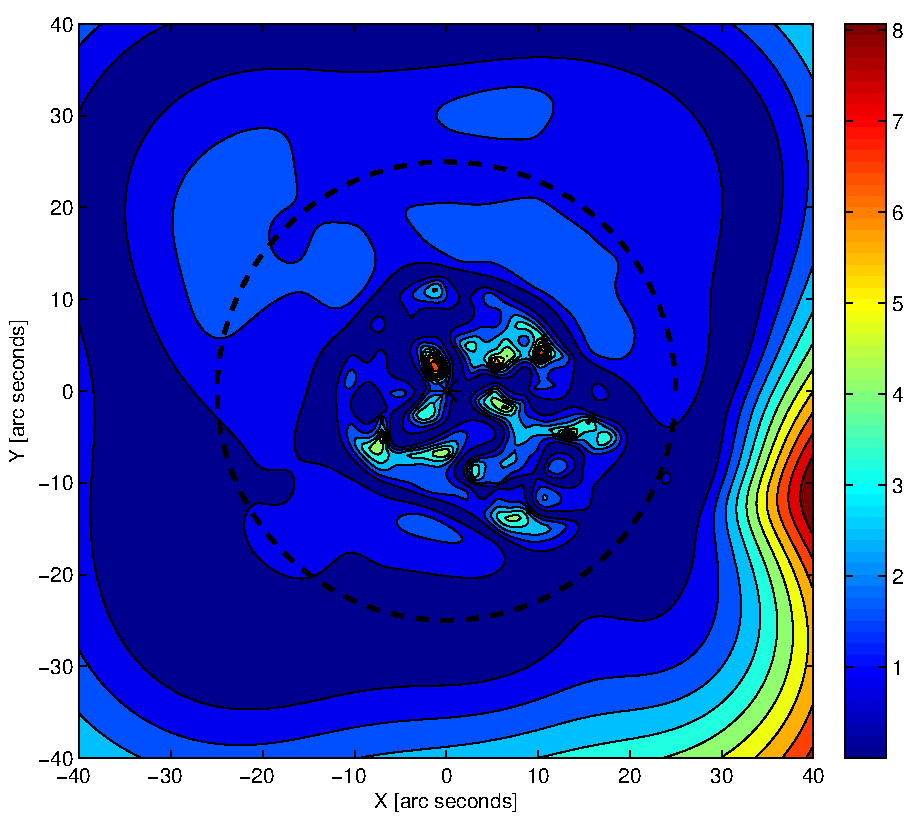
\includegraphics[width=0.32\linewidth]{figures/p1-figures/error25sources5plummer.pdf}\\

  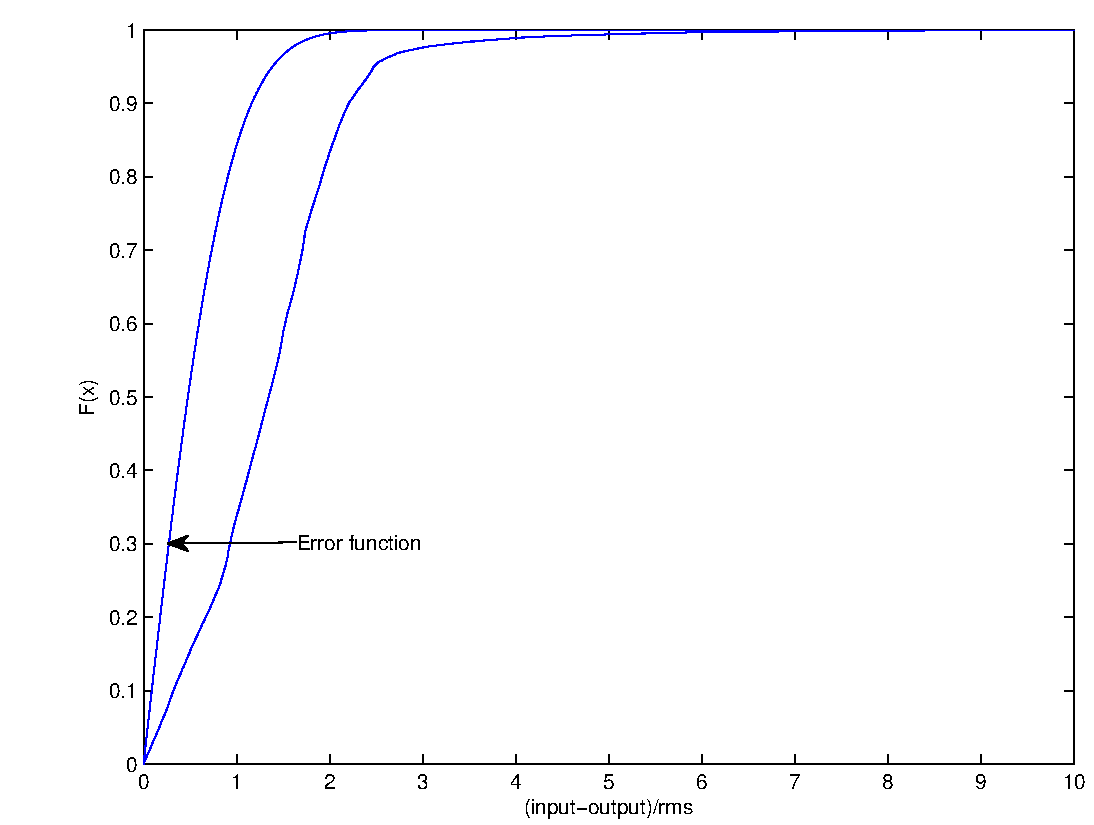
\includegraphics[width=0.32\linewidth]{figures/p1-figures/histogram_cumulative3sources5plummer.pdf}
  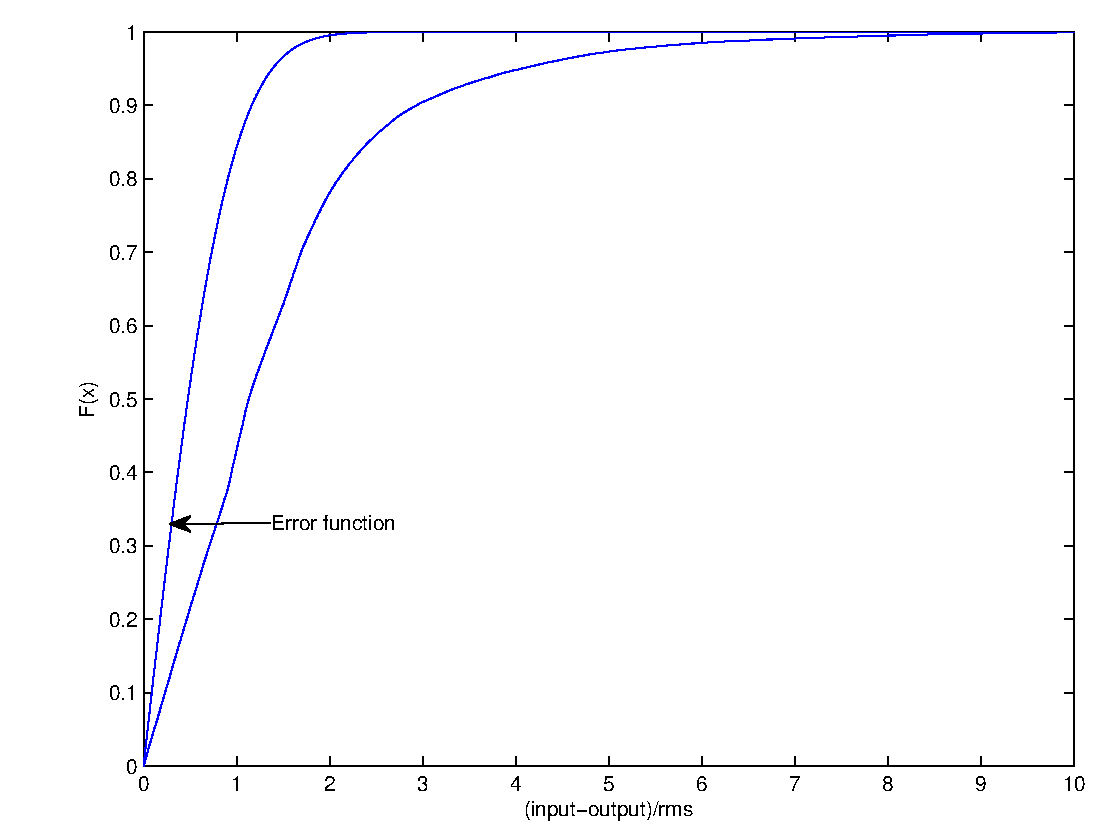
\includegraphics[width=0.32\linewidth]{figures/p1-figures/histogram_cumulative4sources5plummer.pdf}
  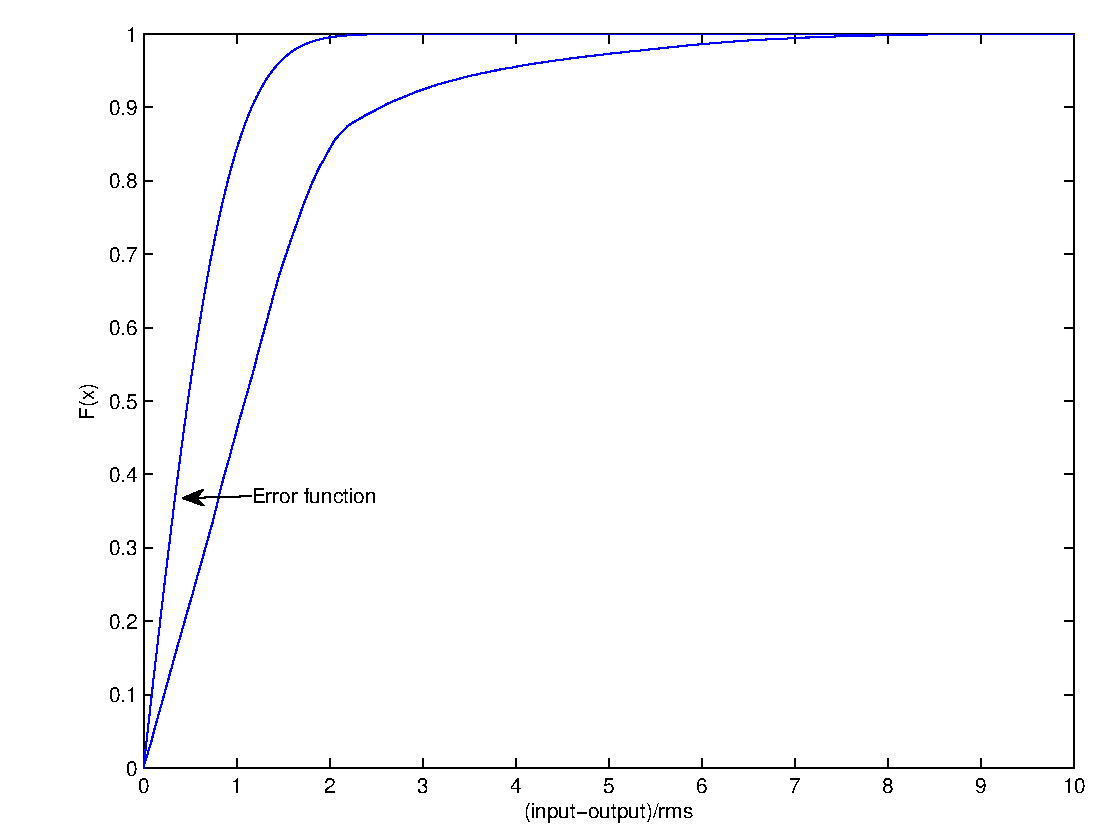
\includegraphics[width=0.32\linewidth]{figures/p1-figures/histogram_cumulative5sources5plummer.pdf}\\
\caption{\label{fig:p1-complex-output} Reconstruction of the lens in
  Figure~\ref{fig:p1-complex-input}. Column~1: using three sources only,
  with the corresponding images shown as black triangles; column 2:
  using four sources; column 3: using all five sources.  The top row
  shows average surface mass density $\Sigma$; units are same as in
  Figure~\ref{fig:p1-plummer-input}.  The second row shows the fractional rms deviation
 of ten reconstructions, $\delta\Sigma/\Sigma$.  The
  third row contains $\Delta\Sigma/\delta\Sigma$ where
  $\Delta\Sigma$ is the pixelwise difference between the true map and
  the average reconstructed map.  The bottom row shows the cumulative
  $\Delta\Sigma/\delta\Sigma$, along with the corresponding curve
  (marked `error function') for Gaussian errors with dispersion
  $\delta\Sigma$.  We conclude that the error estimate $\delta\Sigma$
  needs to be multiplied by $\sim 2$ (or increased by 0.30 on a
  $\log_{10}$ scale).  The worst cases are some very small regions
  (red in the lower panels) where $\log_{10} \Delta\Sigma$ should be
  increased by $\sim+1$.}
\end{figure}

\clearpage

\section{Reconstruction of three real clusters}

In this Section we do mass reconstructions of three galaxy-clusters,
and present these with their accompanying mass error maps. The two
sets of maps for each cluster allow us to judge whether
light-follows-mass (LFM) is a good assumption. We defer the discussion
of the implications of the deviations from LFM to Section~\ref{sec:p1-discussion}.

\subsection{Abell 3827}

Abell 3827 is a lensing cluster at redshift $0.099$.  Three multiply
lensed image systems have been identified \citep{2010ApJ...715L.160C}
belonging to three sources at redshift $0.204$, most probably different
parts of the same source. Another big arc is identified belonging to a
source at redshift $0.408$, but its multiply imaged counterpart has not
yet been identified.  A mass map based on these images
\citep{2011MNRAS.415..448W} indicates a dark extended clump, offset by
$\sim 6\rm\,kpc$ from the brightest of the four or five ellipticals in
the cluster core. This offset, if confirmed, would afford us a unique
opportunity to examine and understand the dynamics in dense regions of
clusters.  One of the primary goals of this paper is to assess the
reality of this offset and estimate its statistical
significance. GRALE is a very different lens mass reconstruction
method from the one used in \cite{2011MNRAS.415..448W}, so detecting
the offset with GRALE will lend credence to its reality.

Using the identified images we reconstructed the mass distribution in
two ways, and then combined the results.  These are displayed in the
three rows of Figure \ref{fig:p1-a3827}.

First, we used the three image systems belonging to the sources at
redshift $0.2$.  The first panel of the top row of Figure
\ref{fig:p1-a3827} shows a spur in the mass map, which is offset from the
nearby elliptical galaxy (the right most of the five grey dots). The
spur's location is similar to the location of the local overdensity
reported in \cite{2011MNRAS.415..448W}, so the offset is similar in
both reconstructions. From the map of fractional rms deviation
$\delta\Sigma/\Sigma$ (right panel of the first row) the spur appears
to be significant; the rms deviation in that region is about $0.1$ kg
m$^{-2}$, and so the fractional error is about 10\%. Since the
structure appears to be extended and not a single clump, it is not
obvious how to quantify it.  We can nonetheless test its significance.
We chose a circle of radius $5''$ (green circle) around the nearby
elliptical.  (The choice of size is somewhat arbitrary; other choices
would also serve our purpose.)  We then calculate the centre of mass
within this circle, for each mass map within the ensemble, and mark
them with green `$+$' signs in the middle panel of top row, which is a
zoom on to the relevant region.  All ten centroids are consistently
displaced from the nearby galaxy (grey circle), by about $1.2''$. The
average of the ten centroids is marked with a blue star symbol.  We
may interpret these results as a hypothesis test.  The null hypothesis
is that the cluster has no mass/galaxy offset, and the mass is centred
on the galaxy light.  A mass reconstruction could nonetheless put the
aperture centroid displaced from the galaxy, simply from the
stochastic element in the genetic algorithm --- note that the mass
reconstructions are not given any information about the cluster
galaxies.  If there is no mass offset, the model offsets would be
random, and the change of all 10 mass reconstructions having an offset
in the same direction would be only 10\%.  But the aperture centroids
are consistently offset in the same region.  Hence there does appear
to be an offset, significant at 90\% confidence, between the mass spur
and the galaxy.

Second, we used all four image systems: three belonging to the sources
at redshift $0.2$ and one with source redshift $0.4$. As mentioned
before, no image counterpart of the latter has been identified, but
there is a possibility of such a counter-image near the centre of the
cluster.  Accordingly, we allowed GRALE to produce extra images in
that region.  The corresponding mass maps are shown in the second row
of Figure~\ref{fig:p1-a3827}. This time the extent of the image region is
larger, and the fraction rms between reconstructions (right panel) is smaller
in the general region of the image at $z_s=0.4$.  A clear mass subpeak
is seen near the elliptical, offset from it by $\sim4''$ or $\sim 7
\rm\,kpc$.  To be consistent with the previous case, we again
calculate the centre of mass, or centroid, in a circular region of
radius $5''$.  Individual centroids are marked with green `$\times$'
signs, and their average is the blue star. Again the offset is detected
at a significance similar to the one above.

Finally, we then combined the two sets of ensembles described above,
for a total of twenty individual maps.  The bottom row of
Figure~\ref{fig:p1-a3827} shows the average mass map, and the map of
$\delta\Sigma/\Sigma$ for the combined ensemble.  The conclusion
remains unchanged.


\begin{figure}[p]
  \centering
  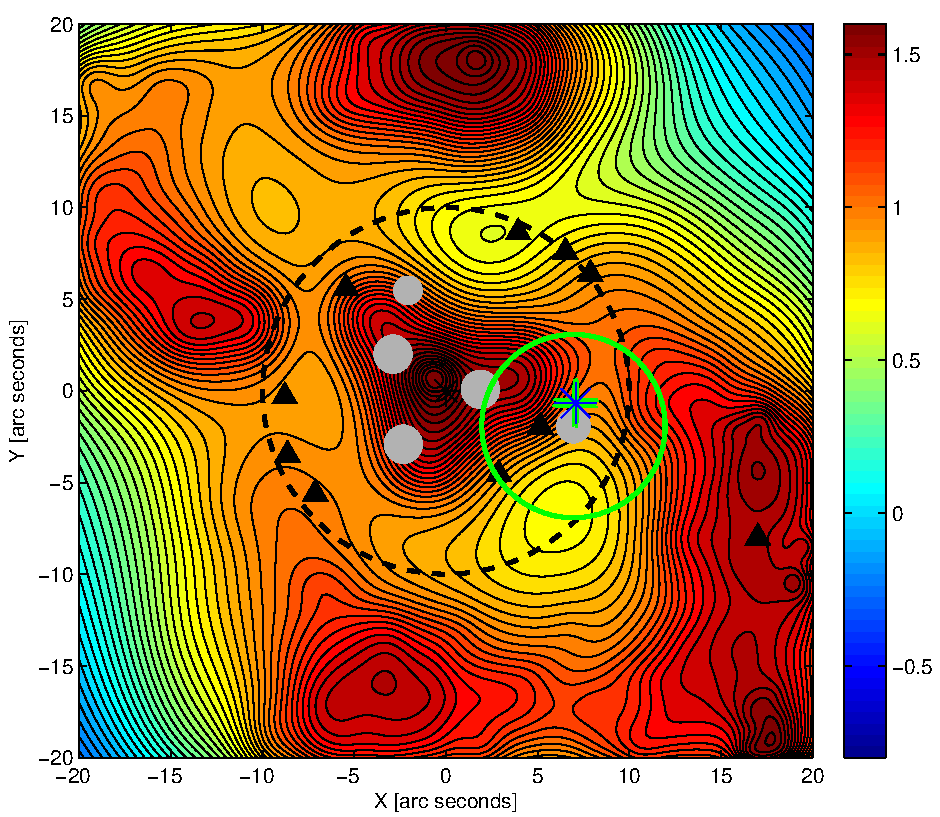
\includegraphics[width=0.24\linewidth]{figures/p1-figures/avg_3sourcesa3827.pdf}
  \hfill
  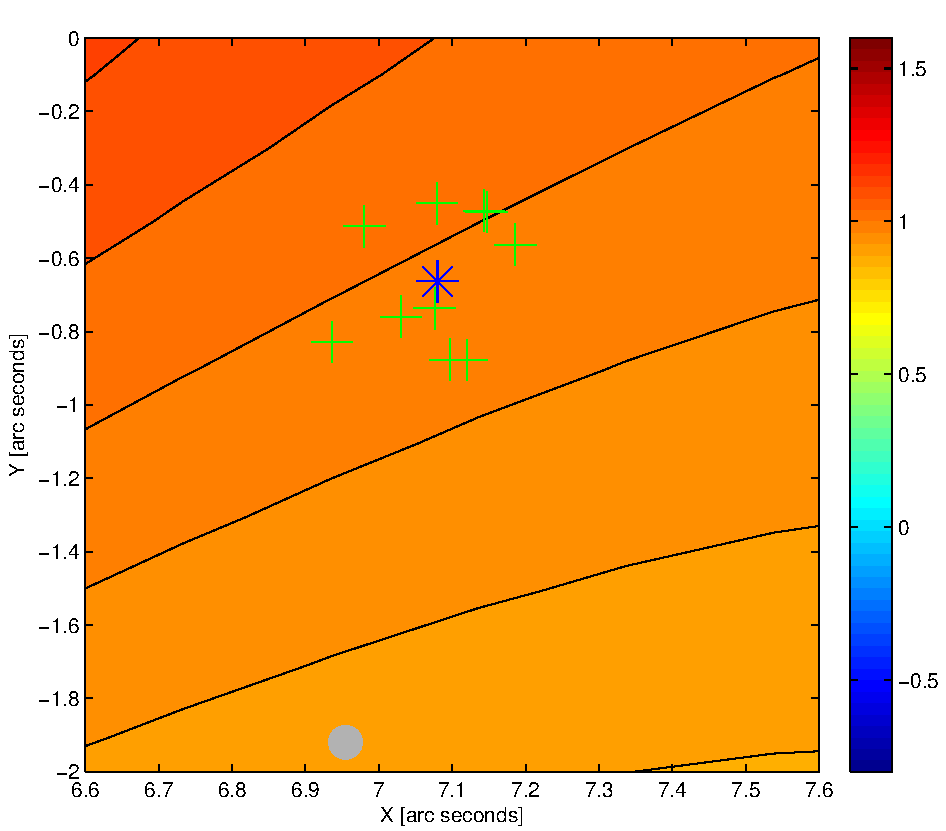
\includegraphics[width=0.24\linewidth]{figures/p1-figures/avg_3sources_zooma3827.pdf}
  \hfill
  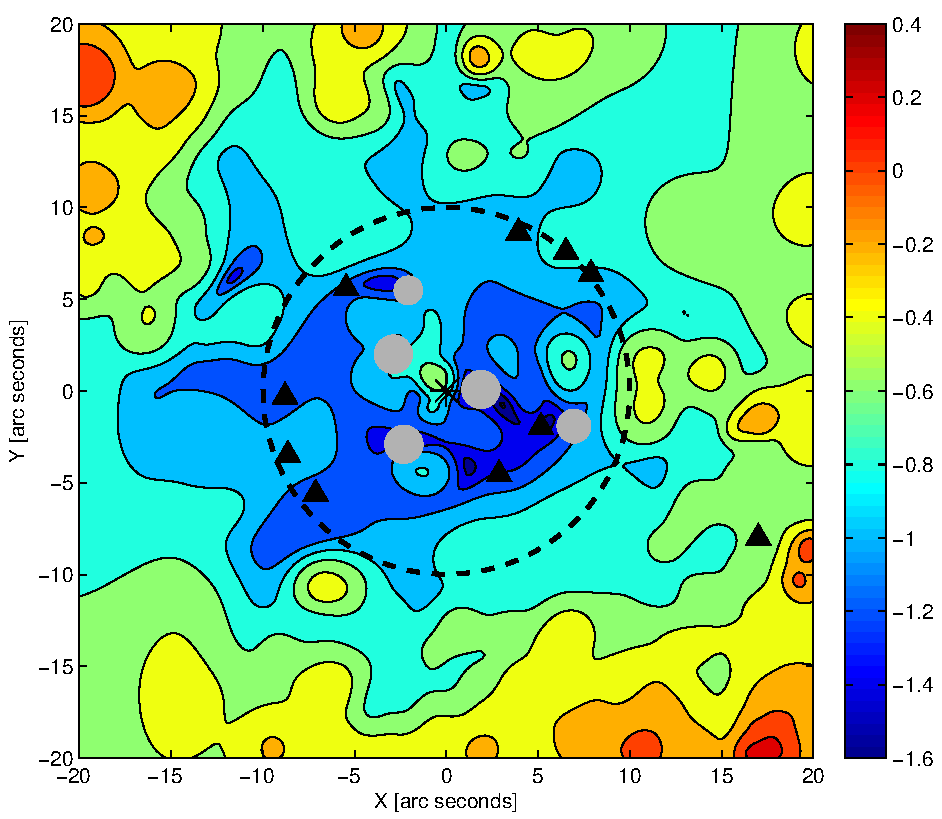
\includegraphics[width=0.24\linewidth]{figures/p1-figures/uncertainity3sourcesa3827.pdf}\\
  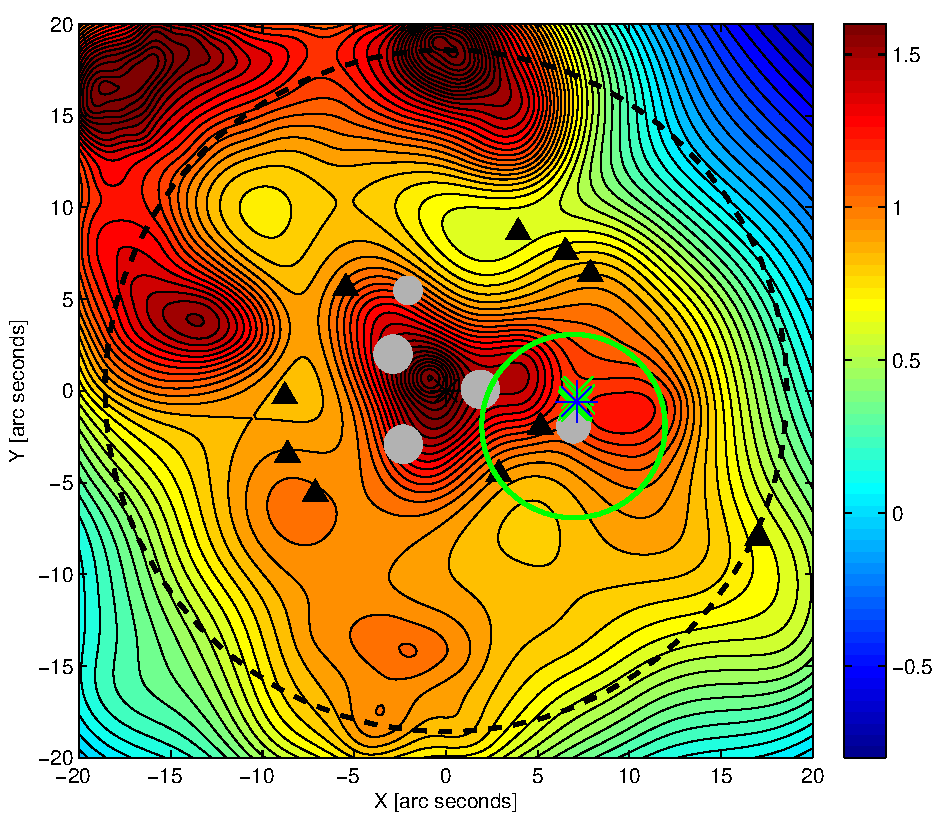
\includegraphics[width=0.24\linewidth]{figures/p1-figures/avg_4sourcesa3827.pdf}
  \hfill
  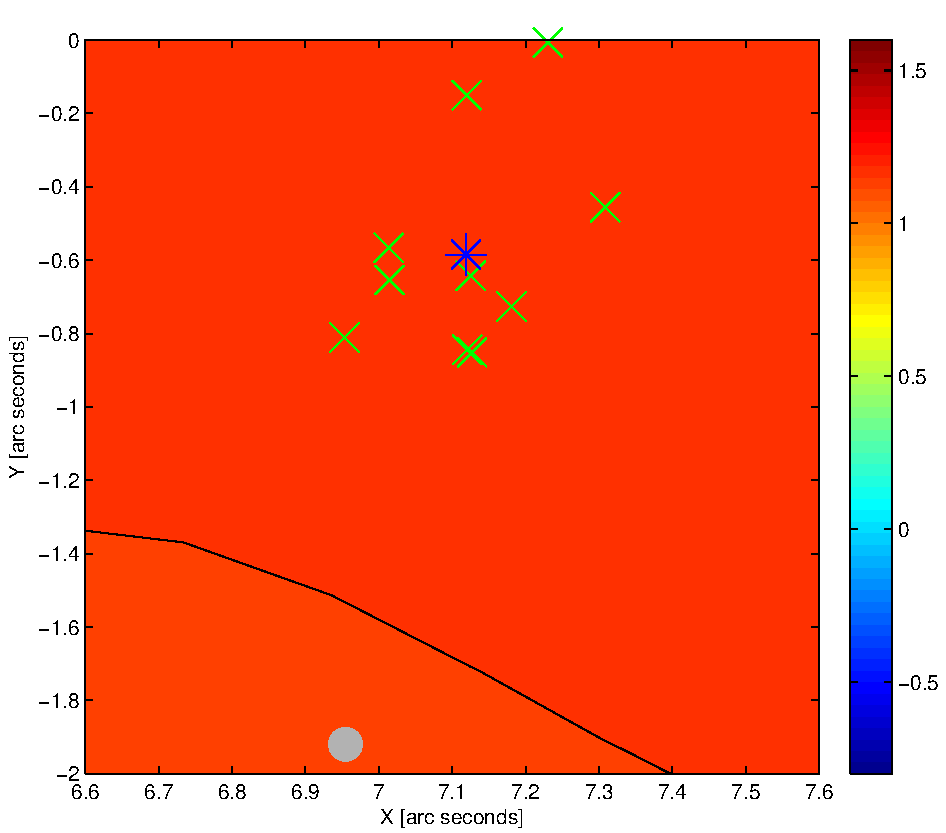
\includegraphics[width=0.24\linewidth]{figures/p1-figures/avg_4sources_zooma3827.pdf}
  \hfill
  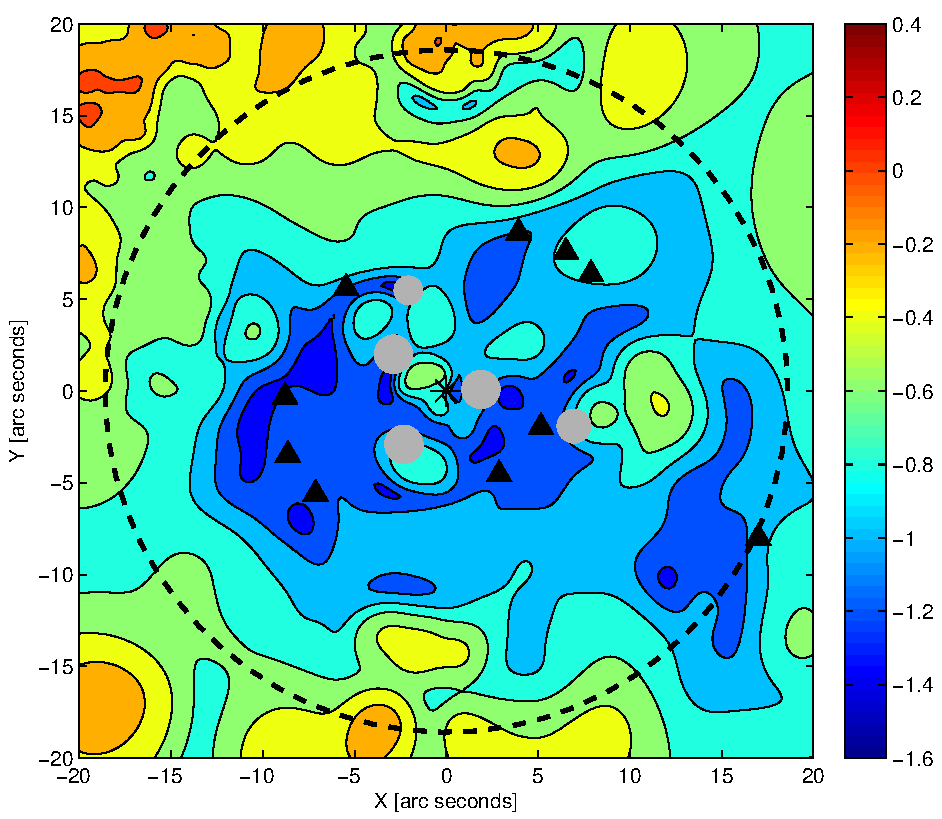
\includegraphics[width=0.24\linewidth]{figures/p1-figures/uncertainity4sourcesa3827.pdf}\\
  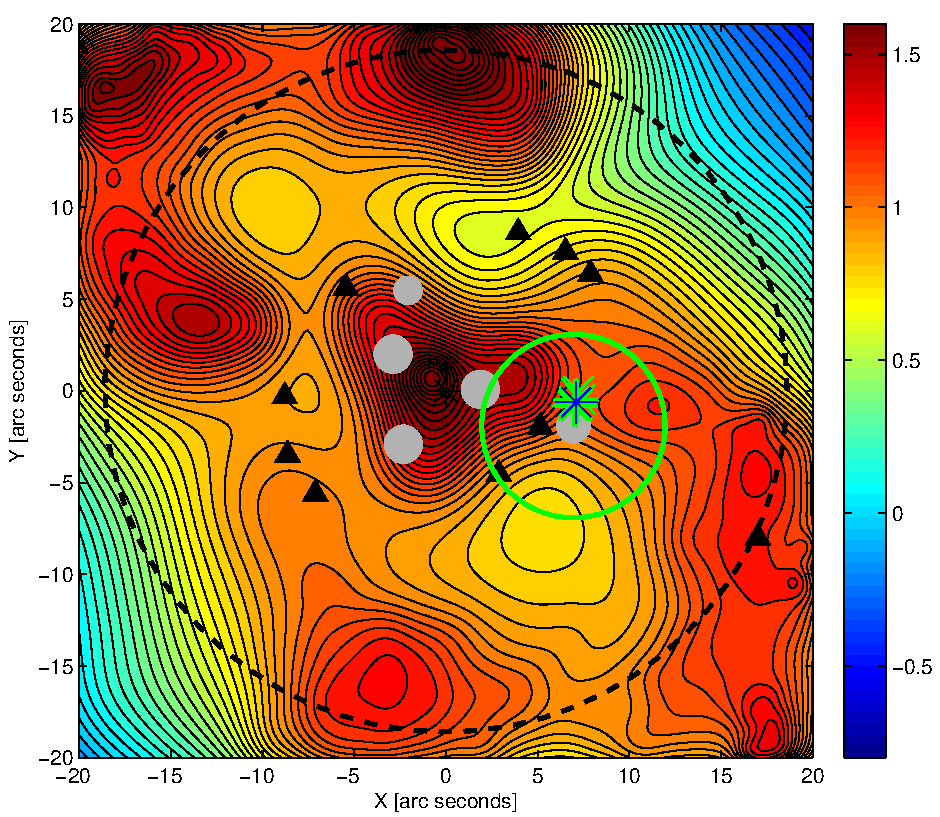
\includegraphics[width=0.24\linewidth]{figures/p1-figures/avg_34sourcesa3827.pdf}
  \hfill
  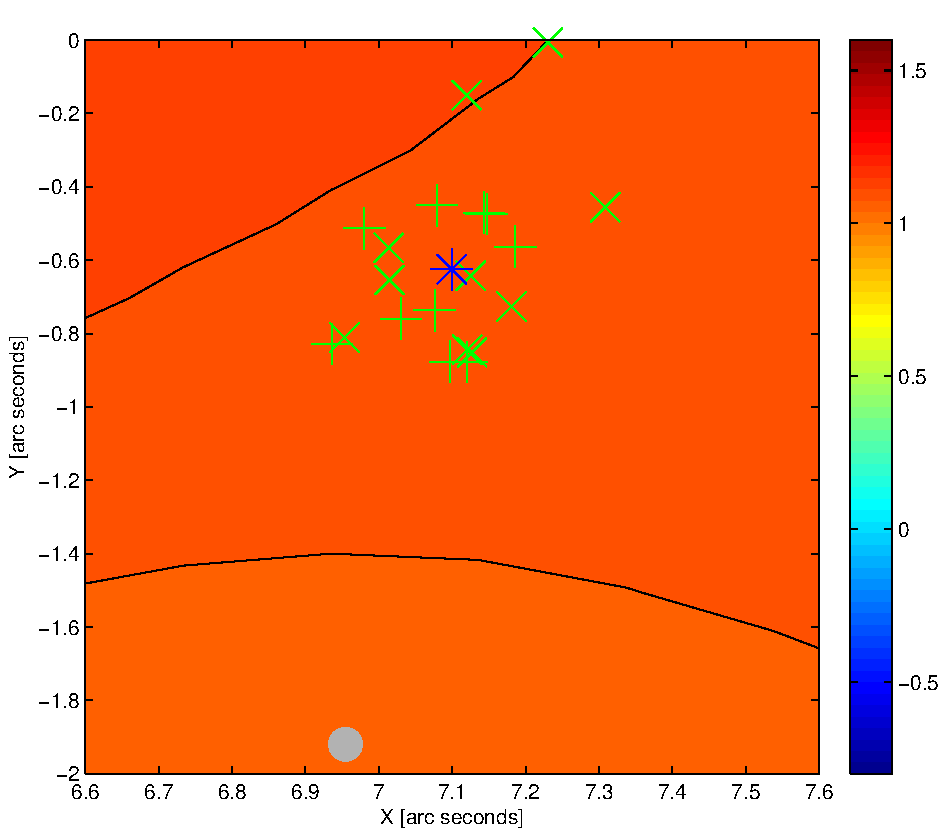
\includegraphics[width=0.24\linewidth]{figures/p1-figures/avg_34sources_zooma3827.pdf}
  \hfill
  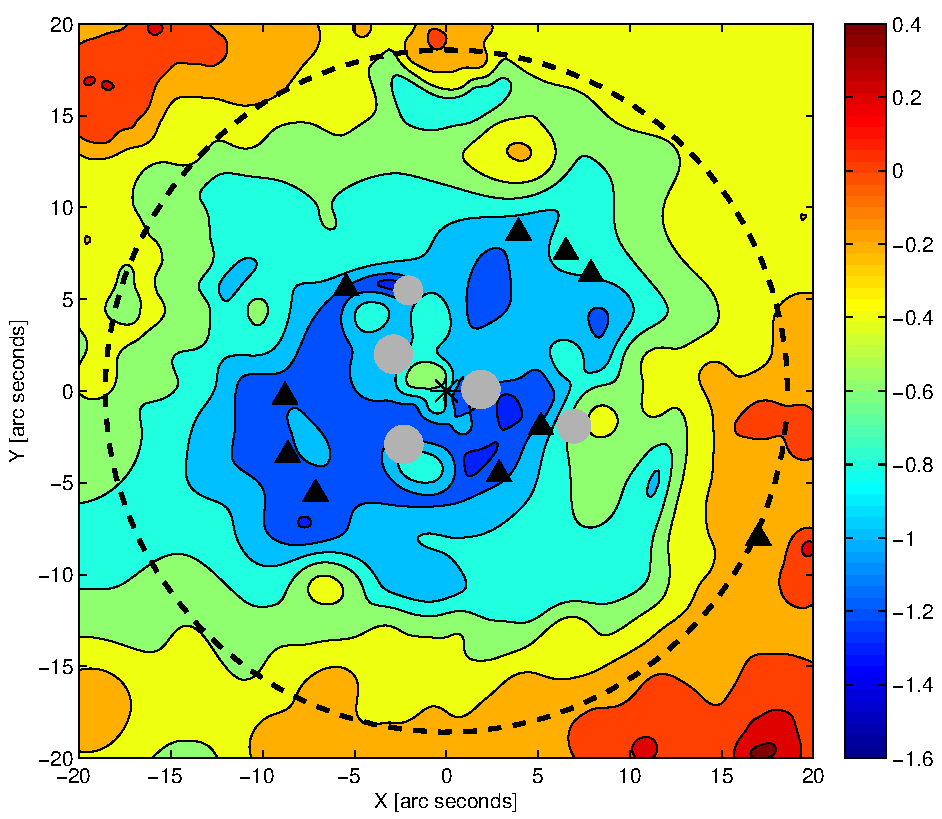
\includegraphics[width=0.24\linewidth]{figures/p1-figures/uncertainity34sourcesa3827.pdf}
\caption{\label{fig:p1-a3827} Mass reconstructions of A3827. North is up
  and East to the right. The scale is 1.82~kpc/arcsec. The upper row
  maps are an ensemble of ten maps, each obtained using only the nine
  images of the source at $z_s=0.2$.  The middle row shows an ensemble
  of ten maps, using nine images of the $z_s=0.2$ source and the
  single image at $z_s=0.4$.  The bottom row combines both ensembles.
  The left column presents the average of the ten mass maps. The
  middle column is a zoom centered on the most luminous elliptical
  N1. The ten green `$+$' signs (top row) and `$\times$' signs (middle
  row) represent centroids from ten individual maps of the mass within
  the green circle shown in the left column. The grey dot towards the
  bottom of the plots (in the middle column) is N1.  The blue asterisk is the centroid of the
  average of the ten realisations.  The right column shows the fractional rms deviation
 between the ten maps, $\delta\Sigma/\Sigma$.}
\end{figure}

\clearpage

\subsection{Abell 2218}

Abell 2218 is a well known and much studied lensing cluster
\citep[e.g.,][]{1998AJ....116.1541A}.  Like other rich clusters, it
has been used in the recent years as a cosmic telescope
\citep{2010A&A...518L..17A,2010ApJ...716L..45H,2010ApJ...709..210K} to
get a better view of distant or faint galaxies.  The strong lensing
region is somewhat larger on the sky than in Abell 3827, and the
greater redshift, $z_l=0.175$, implies a larger physical scale, $3$
kpc arcsec$^{-1}$.

We reconstructed the cluster using the four most secure strong lensing
systems.  Figure~\ref{fig:p1-a2218} shows the mass map (left panel) and
fraction rms dispersion between the ten individual maps of the ensemble 
(right panel).  While apparent offsets are visible between galaxies 
(grey dots) and mass in the central region of the cluster, these are not
significant, because rms in that region is comparable to the typical
value of the surface mass density.  Significant offsets are seen
around the lower right mass clump, where the rms dispersion between
mass maps is low. In the central panel we show a zoom of that region,
similar to that in the middle panel of Figure~\ref{fig:p1-a3827}.  The
green `$+$' signs represent the local mass peaks (not centroids as in
the case of A3827) of individual reconstructions, which are displaced
from the nearest cluster galaxies, represented by grey dots in the
upper right of that panel.

\begin{figure}[p]
  \centering
  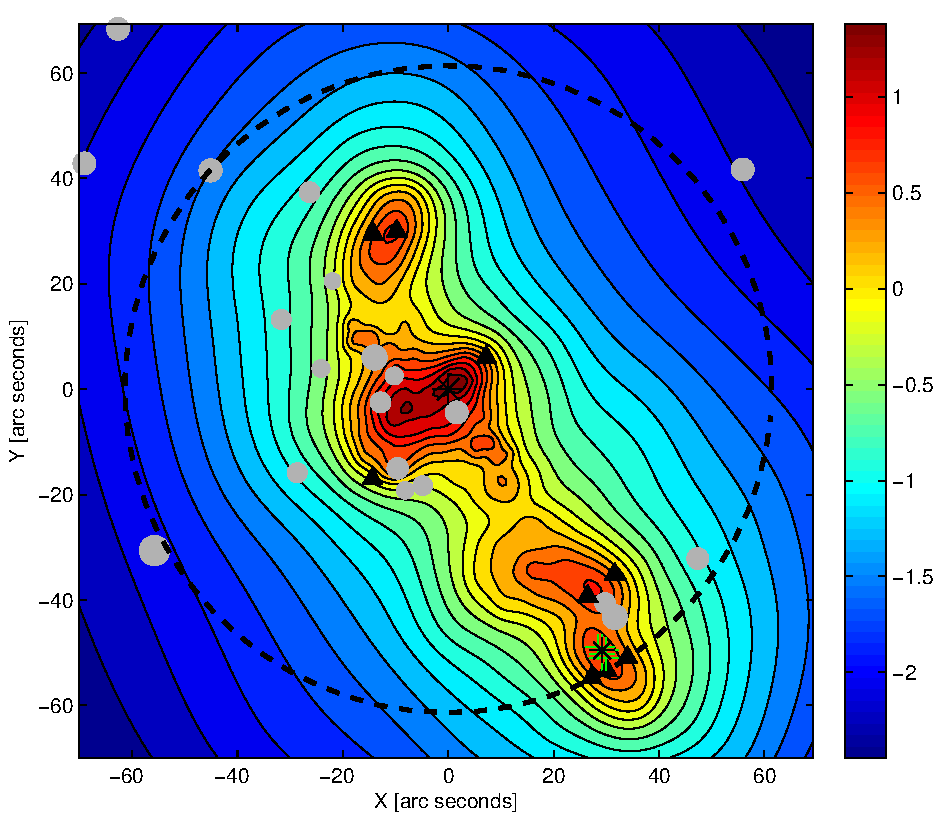
\includegraphics[width=0.32\linewidth]{figures/p1-figures/averagea2218.pdf}
  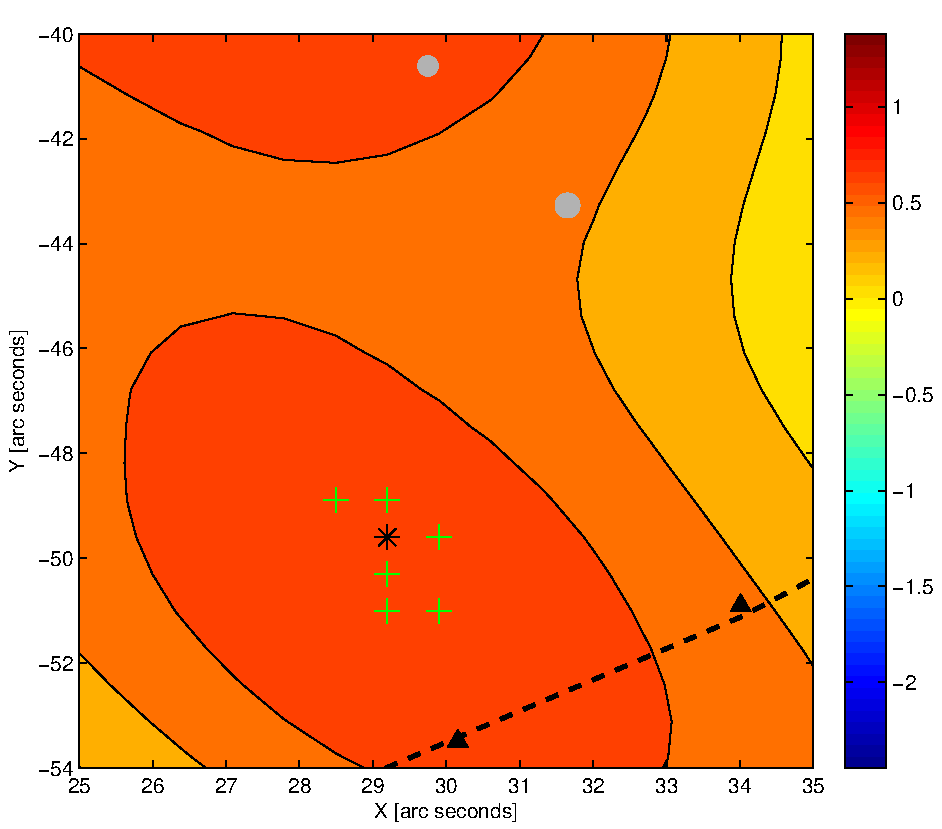
\includegraphics[width=0.32\linewidth]{figures/p1-figures/averagezooma2218.pdf}
  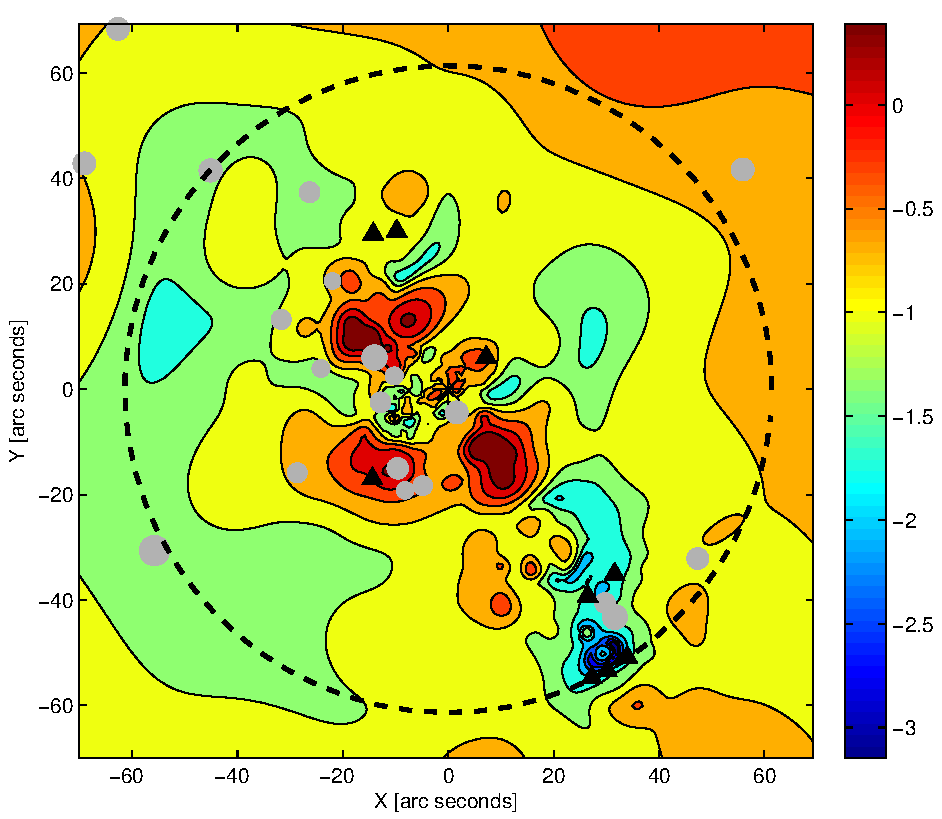
\includegraphics[width=0.32\linewidth]{figures/p1-figures/uncertaintya2218.pdf}
\caption{\label{fig:p1-a2218} Mass map of A2218.  North is up and East to
  the right.  The average mass map (left column) and fractional rms (right column) are
  based on ten realisations. The central column shows the zoom of the
  region with mass-light offsets, and the green '+' signs are the
  local mass peaks from individual reconstructions. The scale is
  3~kpc/arcsec.  Galaxies with $R<20$ \citep{1992A&A...266....6P} are
  marked with grey dots.}
\end{figure}

\clearpage

\subsection{Abell 1689}

Abell 1689, at redshift $0.183$, is perhaps the best known lensing
cluster, containing over a hundred lensed images from at least thirty
background sources extending to high redshifts
\citep{2005ApJ...621...53B}.  Our reconstruction of its mass is shown
in Figure \ref{fig:p1-a1689}.  As with Abell 2218, the mass map and the
rms maps are in the left and right panels. There are no significant
mass/light offsets in this cluster. To illustrate that, in the central
panel we show a zoom into the central region, where the mass peaks of
the ten individual maps are shown as green '+' symbols. Their
distribution with respect to the central cluster galaxy (grey dot) is
consistent with the two being coincident.

Because the cluster has many multiply imaged systems spanning a wide
range of redshifts it is possible to test if there are line of sight
(los) structures that have affected the positions of images. We
divided the multiply lensed sources into two groups, the low redshift
system (LRS) and high redshift system (HRS). LRS consists of a total
of three multiply imaged systems with five, three and three (total of
eleven) images at redshifts 2.54, 1.99 and 1.98, respectively.  HRS
consists of a total of two multiply imaged systems with two and five
(total of seven) images at redshifts 4.53 and 2.99, respectively. We
then carried out mass reconstruction for A1689 using LRS and HRS
separately.  The two mass maps are shown in
Figure~\ref{fig:p1-a1689-los}, in the upper left and upper middle
panels, respectively. The corresponding fraction rms distributions are shown
below each map.  The upper right panel is the difference between HRS
and LRS maps divided by the rms of the LRS maps ($\Delta \Sigma/\delta\Sigma$).  
Most of this map is consistent with a uniform surface
mass density of low amplitude, about a factor of ten below the
critical surface mass density. This could be due to steepness, or mass
sheet degeneracy which affected one map more than the other. The only
prominent feature is a mass excess in the HRS map, compared to the LRS
map, centred at around $(-20'',\,35'')$.  The $\delta\Sigma$ maps for both 
HRS and LRS are both low in that region, suggesting that the structure is
real. We interpret this feature as a los structure, probably in the
redshift range 2--3.  Another test of the structure's significance is shown
in the lower right, which contains a histogram of the upper right plot 
$\Delta\Sigma /\delta\Sigma$ (pixelwise). 
The putative los structure contributes to the tail extending beyond
the right edge of the distribution.
The corresponding lensing mass would be $\sim10^{13}M_\odot$ if the
structure were at the same same redshift at A1689, but since the
structure can only be at $z>2.5$, the critical density and hence the
lensing mass are much lower --- a few times $10^{12}M_\odot$ ---
amounting to a modest galaxy group.  There is another feature at
$(-50'',\,-60'')$, but it is outside the image circle, and the $\delta\Sigma$
in that region says that it is not significant.



%%%%%%%%%%%%%%%%%%%%%%%%%%%%%%%%%%%%%%%%%%%%%%%%%%%%%%%%%%%%%%%%%%%%%%%%%%

\begin{figure}[p]
  \centering
  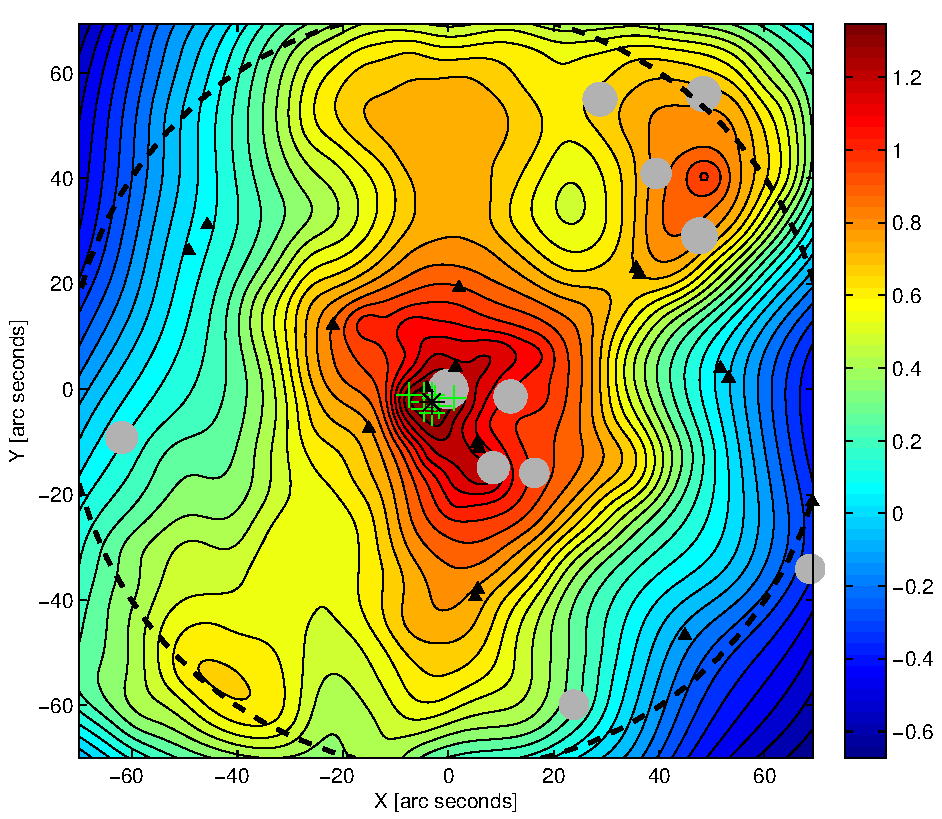
\includegraphics[width=0.32\linewidth]{figures/p1-figures/averagea1689.pdf}
  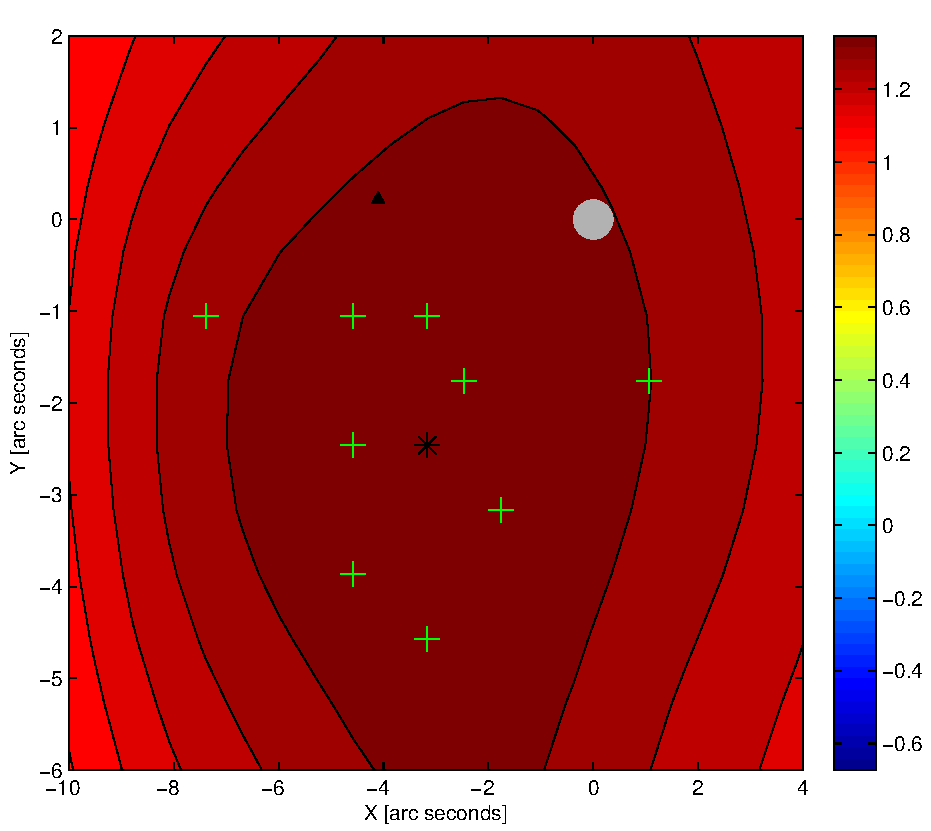
\includegraphics[width=0.32\linewidth]{figures/p1-figures/averagezooma1689.pdf}
  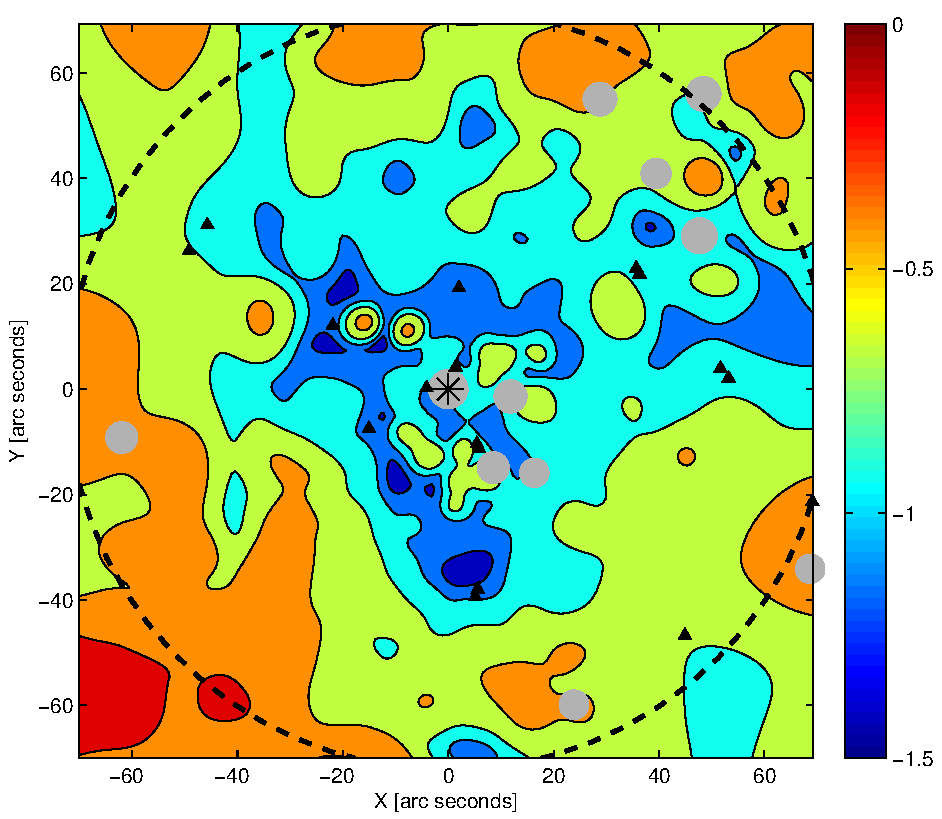
\includegraphics[width=0.32\linewidth]{figures/p1-figures/error1a1689.pdf}
 \caption{\label{fig:p1-a1689} Mass maps of A1689.  North is up and East
   to the right. The columns are similar to those in
   Fig.~\ref{fig:p1-a2218}. Galaxy positions \citep{2002A&A...382...60D}
   also marked.}
 \end{figure}

\begin{figure}[p]
  \centering
  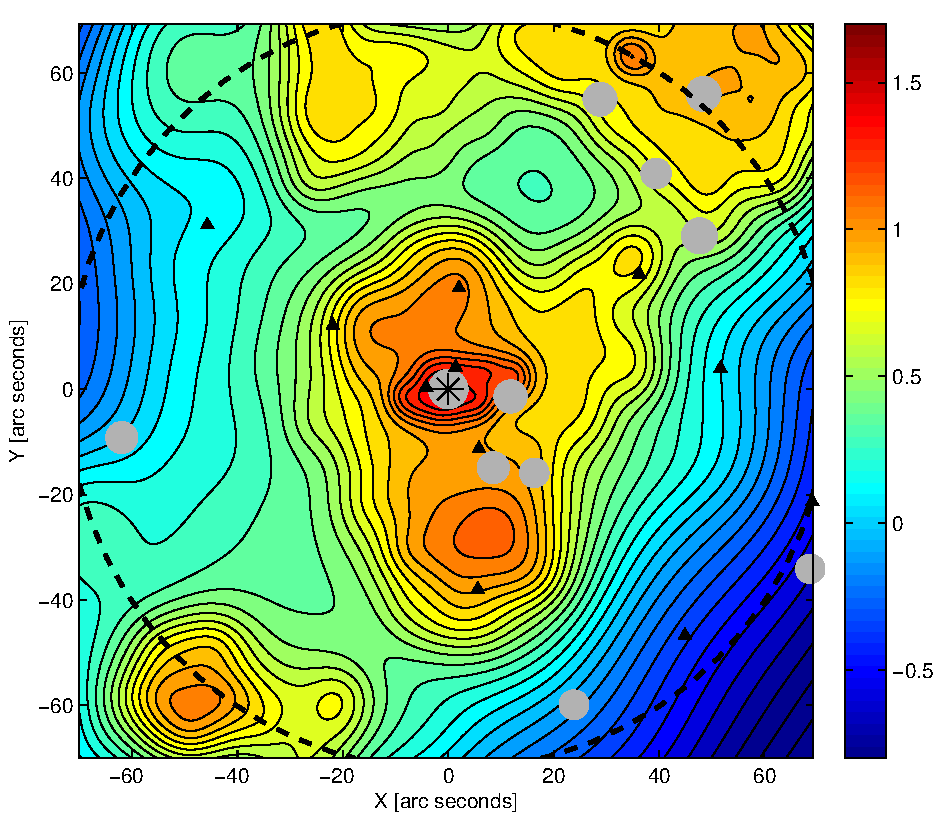
\includegraphics[width=0.32\linewidth]{figures/p1-figures/low_za1689.pdf}
  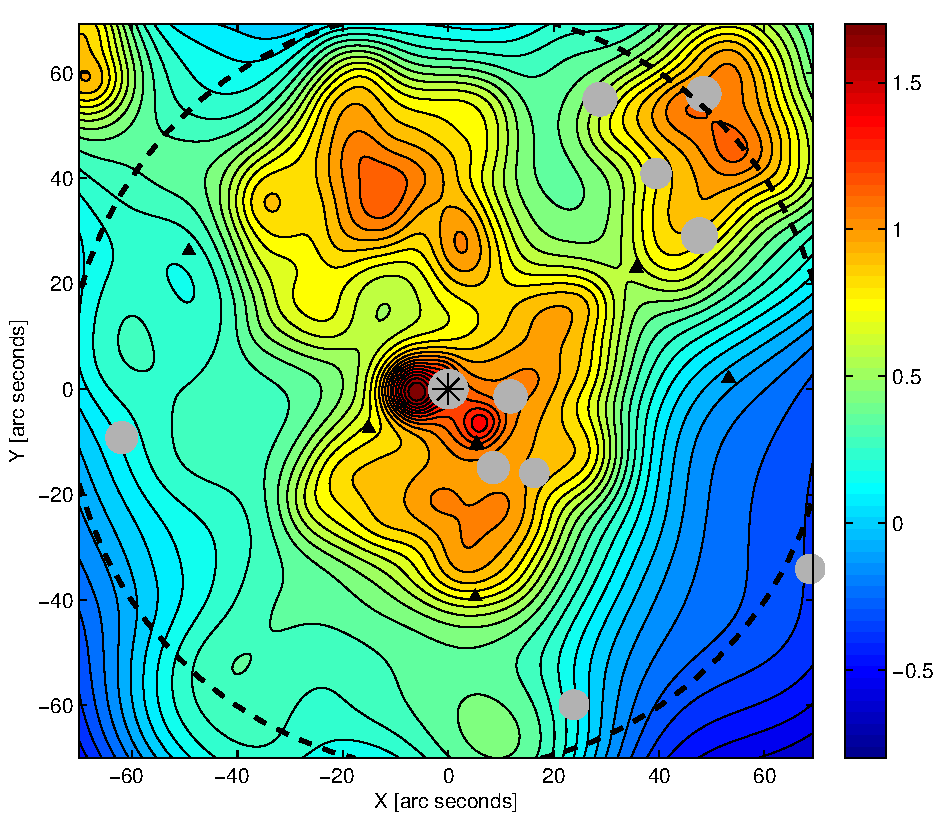
\includegraphics[width=0.32\linewidth]{figures/p1-figures/high_za1689.pdf}
  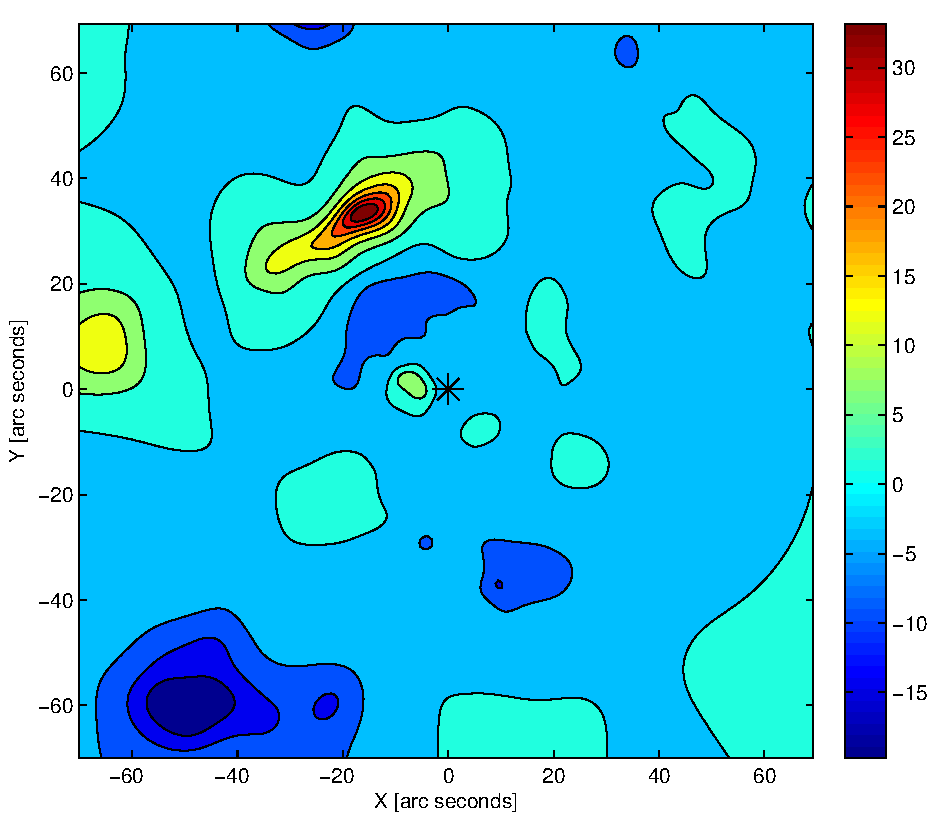
\includegraphics[width=0.32\linewidth]{figures/p1-figures/high_low_rmsa1689.pdf}\\
  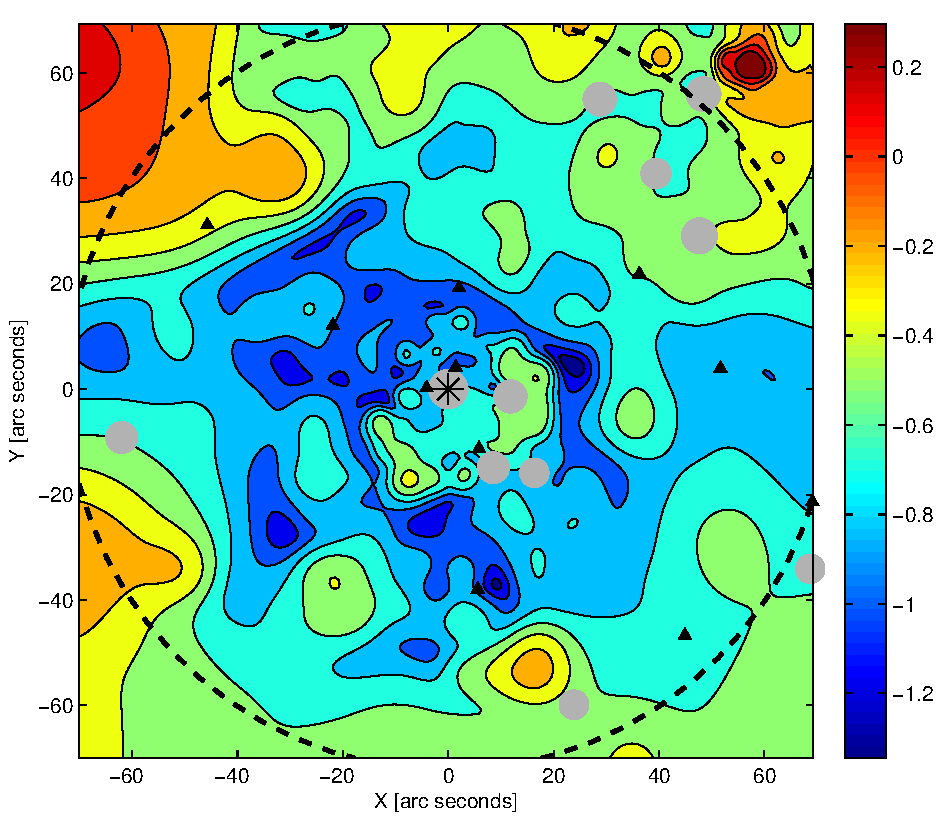
\includegraphics[width=0.32\linewidth]{figures/p1-figures/error1a1689lowz.pdf}
  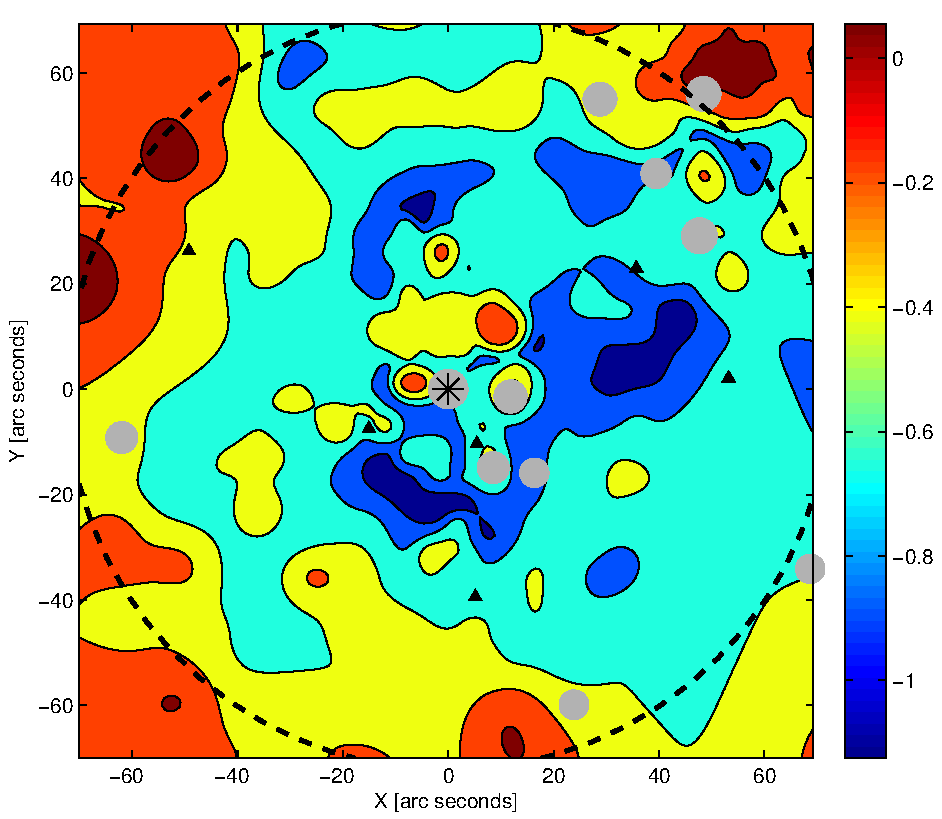
\includegraphics[width=0.32\linewidth]{figures/p1-figures/error1a1689highz.pdf}
  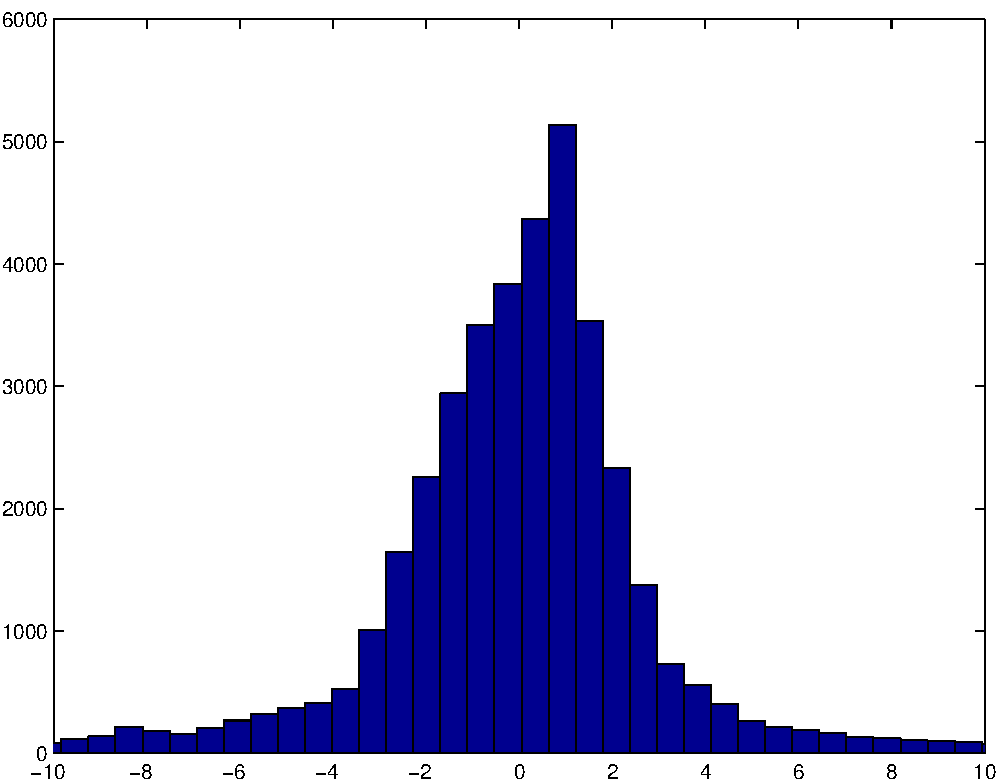
\includegraphics[width=0.32\linewidth]{figures/p1-figures/histograma1689los.pdf}
\caption{\label{fig:p1-a1689-los} Test for the line of sight structure in
  A1689.  Upper left and upper middle panels are the mass maps
  obtained using two separate sets of sources: at low and high
  redshifts respectively. Lower left and lower middle panels are the
  corresponding fractional rms maps. Upper right is the difference between the
  high-$z$ (HRS) and the low-$z$ (LRS) maps divided by the rms
 of the low-$z$ maps  (i.e., $\Delta\Sigma/\delta\Sigma$, which is dimensionless); the scale is linear. Note the apparent structure at higher $z$,
  near $(-20'',\,35'')$.  Lower right is the histogram of the map above it (pixelwise) $\Delta\Sigma / \delta\Sigma$.}
\end{figure}

\clearpage

\section{Discussion}\label{sec:p1-discussion}

Gravitational lensing offers a unique opportunity to study the
distribution of matter in clusters of galaxies. Free-form
reconstruction methods take full advantage of this.  Our synthetic
tests show that GRALE recovers the mass distribution well, and the
concomitant errors provide a reliable guide to assessing the
significance of various mass features. The test case in Figure
\ref{fig:p1-plummer-output} and \ref{fig:p1-complex-output} shows no spurious offsets in the mass maps.

Reconstructions of the three real lensing clusters indicate some
curious features.  In two clusters we see offsets between the optical
light and the nearest mass concentrations.  The form of the offsets is
not resolved: they could be distinct peaks in the projected mass
distribution; or they could be spurs that extend from a peak that
itself coincides with the galaxy light; or the offsets could very
lopsided dark halos around galaxies.  (We emphasize that not all
offsets seen in the reconstructed mass maps are significant, but only
those that pass the statistical significance tests.)  A caveat to bear
in mind is the assumption that the observed image positions are
accurate. Because lensed images are often faint, have low surface
brightness and are superimposed on brighter cluster galaxies, image
identification is not always straightforward. It is thus conceivable
that some images have been misidentified.  But assuming the image
identifications are all valid, confirmation by independent techniques
is desirable.  Lens reconstruction methods not assuming light traces
mass in some way include Lensview \citep{2006MNRAS.372.1187W},
LensPerfect \citep{2008ApJ...681..814C} and PBL
\citep{2008ApJ...687...39D} and any of these would be suitable.  If
the mass/galaxy offsets are confirmed, they would lead to interesting
conclusions about the nature of clusters and dark-matter.

In general, several reasons for offsets are possible. Superimposed, but dynamically unrelated 
line of sight structures could contribute lensing mass, with no apparent associated light, 
especially if the structures are considerably further away from us than the main lensing cluster.  
However, we argue that the offset in A3827,  is not due to the line of sight structure
because of the very low redshifts of the sources. In A2218 line of sight structures are also 
unlikely to be the cause because only a very concentrated and massive los structure can 
contribute significantly in the vicinity of a massive clump within a cluster. Such chance
superposition are expected to be rare. 

Line of sight structures are more likely to make a contribution away from mass concentrations 
within the cluster, where cluster projected densities are lower. This can be illustrated with 
dark-matter N-body simulations. The blue lines in Figure~\ref{fig:p1-simulation} are the isodensity 
contours of the total projected mass in a cylinder centered on a halo whose virial radius is the
radius of the window, while the red lines are the contours of the projected mass inside the 
virial sphere of the cluster. We caution that  these plots were made with a limited line of sight
depth of about comoving 90 Mpc (Simulations courtesy J\"urg Diemand; \cite{2004MNRAS.352..535D}).
The black contours mark regions where the fractional mass excess due to the line of sight 
structures (and not the mass within the virial sphere) amount to $25\%$ of total.  The top two 
panels show examples where the contribution from the los material is typical, while the bottom two
panels present two cases with the most contribution (out of a total of 100 lines of sight). Even though
the length of the cylinder is not large, the plots show that los structures cannot make a significant 
contribution where the cluster density is high. However, such structures can make a significant
contribution at some distance away from the cluster centre.     

\begin{figure}[p]
  \centering
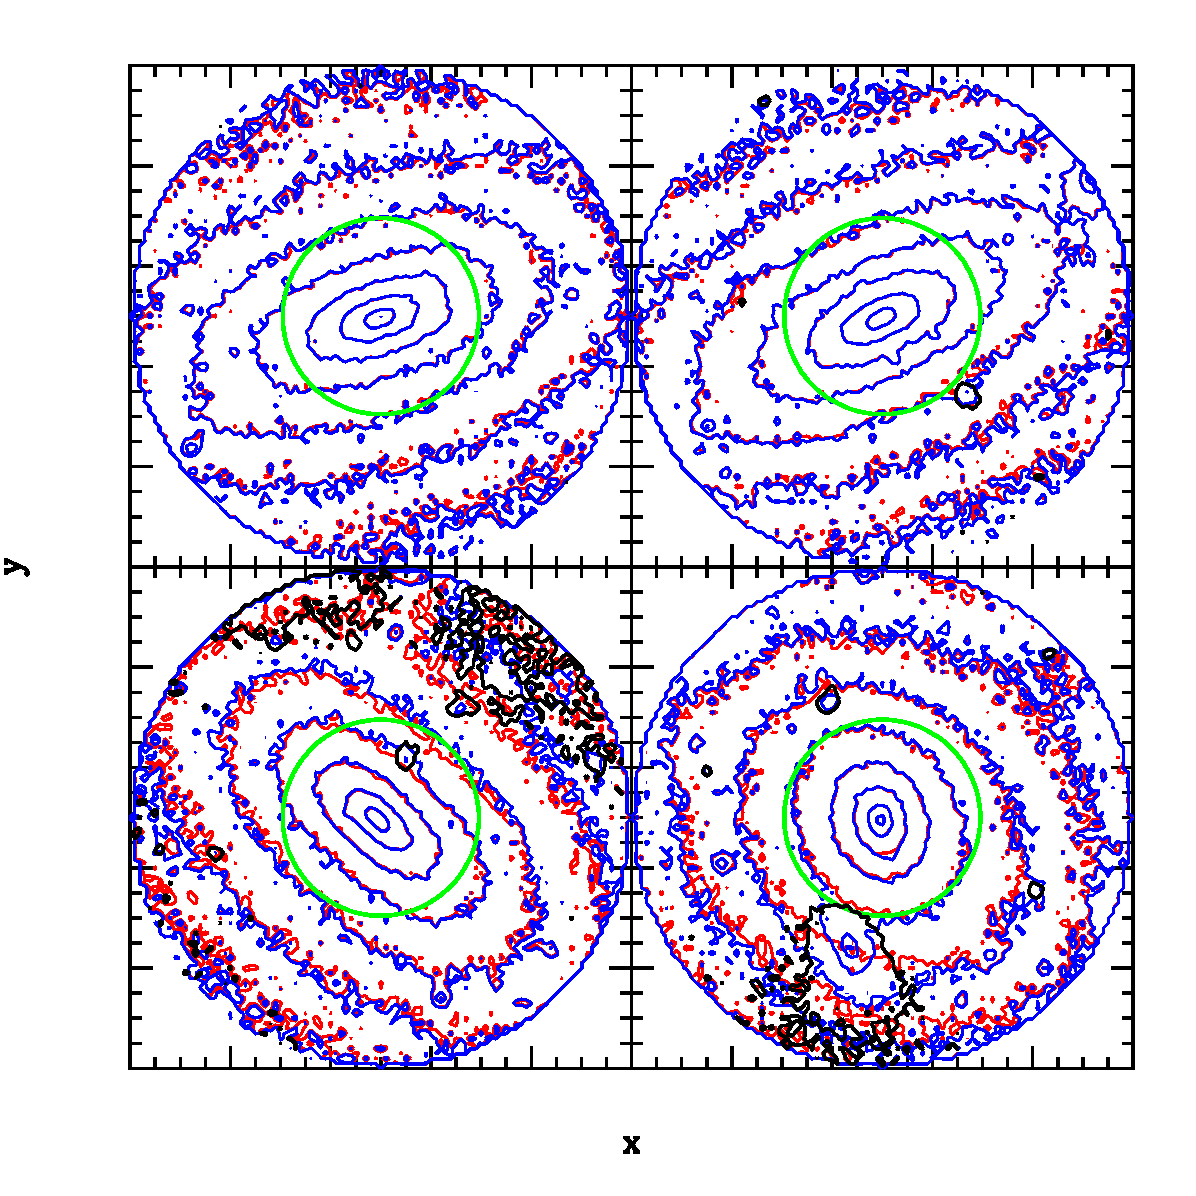
\includegraphics[width=1.0\linewidth]{figures/p1-figures/smfourmass.pdf}
\caption{\label{fig:p1-simulation} Density contours of projected mass centered on halos taken
from dark matter only simulations \citep{2004MNRAS.352..535D}. The radius of the window
is the virial radius, and the green circle marks the typical radius where lensed images will 
be formed. The red density contours are due to the halo mass interior to the virial sphere, 
while the blue contours are due to all projected mass within a cylinder of roughly 90 Mpc. The
black contours mark regions where the fractional mass excess due to the line of sight structures
(and not the mass within the virial sphere) amount to $25\%$ of total.  The top two panels show
average lines of sight, while the bottom panels the two (out of 100) where los material makes the
most contribution.
}
\end{figure}

\clearpage

In A1689 we might be seeing such a line of sight structure. After subtracting the mass 
reconstruction based on high-$z$ sources (HRS) from that based on low-$z$ sources (LRS) we see a 
mass concentration about 30 arcsec, or 100 kpc from cluster center. It is statistically significant
(it contributes to the tail of the distribution shown in Fig.~\ref{fig:p1-a1689-los} which extend beyond the
right edge of the plot) but is not associated with bright cluster galaxies. We interpret it as arising 
from  a structures between the $z\approx 2$ and $3$.

If not line of sight structure, what else can be responsible for mass-light offsets seen in 
A3827 and A2218?  Offsets could be intrinsic to the cluster, and be due to manifestations 
of known physics, like gravity, and hydrodynamics of the gas, or new physics, such as self-scattering 
of dark matter. Offsets in merging clusters have been observed, but mostly between the dark matter and 
the X-ray emitting gas components \citep{2006ApJ...648L.109C,2013MNRAS.429..833H,2012ApJ...758..128C}. 
In the outskirts of Abell 2744 a separation between dark matter and galaxy components is also seen
\citep{2011MNRAS.417..333M}, and in the merging cluster CL0152-1357 an offset between Sunyaev-Zel'dovich 
effect and X-ray peaks has been detected \citep{2012ApJ...748...45M}.  Most of these offsets are
on larger scales then what we detect in this work. For smaller scale offsets early stage mergers are
probably not the cause, and different set of causes has to be considered.

One of the possibly relevant gravitational effects is the oscillation or wobbling of a galaxy, 
such as a BCG around the bottom of the gravitational potential. This has been observed in 
a sample of galaxy clusters as a displacement of the BCG from the lensing centroid
\citep{2012MNRAS.426.2944Z}. The distribution is displacements is wide, and peaks at
roughly 10~kpc.  Whether this is a likely explanation for the offsets in A3827 and A2218 is yet 
to be determined---the observed offsets are not for central cluster galaxies.

It is less likely, but still possible that the offsets are a consequence of tidal effects. 
These would strip the material from the galaxy symmetrically in the leading and 
trailing directions. Since the offsets in A3827 and A2218 do not show such symmetry, 
tidal effects are probably not the main cause.

Dynamical friction would create an asymmetric structure and would preferentially 
distort the distribution of dark matter and not stars if the former has a more extended 
distribution. A numerical simulation would be required to test this possibility.

The formation of a galaxy cluster is a complex process involving hydrodynamics of gas. 
It is possible that  star formation induced by galaxy mergers within clusters would result 
in stars and dark matter halos offsets.

Finally, if dark-matter has non-negligible self-interaction cross-section, dark-matter 
particles of the galaxy halo would experience a drag force as the galaxy moves within
the halo of the cluster. The nature of the resulting dark-matter features induced by these 
interactions may be consistent with those observed in A3827 and A2218, but detailed 
simulations are required \citep{2014MNRAS.437.2865K}.


\section{Acknowledgement}
LLRW would like to acknowledge the hospitality of ITP, Zurich.

%%%%%%%%%%%%%%%%%%%%%%%%%%%%%%%%%%%%%%%%%%%%%%%%%%%%%%%%%%%%%%%%%%%%%%%%%%

% \bibliographystyle{mn2e}

% \def\apj{ApJ}
% \def\apjl{ApJL}
% \def\aj{AJ}
% \def\mnras{MNRAS}
% \def\aap{A\&A}

% \bibliography{ms}


% \end{multicols}

\clearpage


%==============================================================================
% Chapter 3: Paper 2
%==============================================================================

\chapter{An Analytic Model for the Matter Power Spectrum}
\label{p2:chap:analytic-power-spectrum}

\section{Introduction to the Paper}

The future generation cosmological surveys, like Euclid, 
LSST etc., are expected to provide
very large quantity of high quality data such that it will be 
possible to probe small scale structures like never before. Employing 
the cosmological observables from these experiments,
like weak gravitational lensing, baryon acoustic oscillations etc., 
percent level constraints are expected on all cosmological 
parameters. With such tight
constraints, either the $\Lambda$CDM model will gain more credibility
in the community else it would be rejected with higher confidence; either 
way the efforts will be unified. 
In order to employ the full constraining power from these experiments, a good
understanding of non-linear structure formation is needed.
In this paper, we studied an important aspect of this theory -- 
the matter power spectrum. It underlies
many cosmological observables, it is important
to model it accurately and precisely up to the non-linear regime. 

In this paper, we provide an estimator for the matter
power spectrum based on the Zeldovich approximation and the halo model. 
This model is calibrated on $N-$body simulations, and gives
an accuracy of a few percent up to $k\sim 0.8 h^{-1}\mathrm{Mpc}$ 
over a range of cosmological models 
including neutrino masses and redshifts. 

We also provide an estimator for the full covariance matrix of the matter power
spectrum which is very important for statistical inference from the cosmological
data. In spite of the simple form of the covariance estimator, it is found
to be in remarkable agreement with simulations. 

We provide a description of baryonic effects on the matter
power spectrum in this framework. This model can be used to project and estimate
weak lensing power spectrum and utilise the future generation surveys
to put strong and unbiased constraints on the cosmological parameters.

\paragraph{Role:} This project was done under the supervision of Professor Uros Seljak. 
The starting point was analytical calculations using the halo model. The
idea was to expand the 1-halo term in Taylor series, and analytically
evaluate the coefficients. I accumulated 38 matter power spectra
from the cosmic emulator, each for its original cosmological node. I
also evaluated Zeldovich power spectra using code from Zvonimir Vlah
for the same 38 cosmological models and three redshifts (0.0,0.5,1.0).
I fitted the function $A_0 - A_2k^2 + A_4k^4$ to the difference between 
the full matter power spectra and Zeldovich
approximation, and compared
the fitted coefficients with those evaluated analytically from the halo model. 
We found big differences in $A_2$ and $A_4$ coefficients, whereas
$A_0$ remains the same. This shows the divergence of the halo model
from the true matter power spectrum in non-linear scales. 
I found very strong correlation between fitted coefficients and $\sigma_8$,
and therefore we fitted them using a single power law for all three redshifts
and computed the corresponding residuals. 
Further I fitted the residuals for its correlation to the 
effective slope $n_{\rm eff}$.
We provide these fitting functions in the paper to estimate the 
coefficients of the 1-halo term using the cosmological models
and redshifts. Given these fitting functions, we computed the matter
power spectra, and compared them to the original emulator output. 
I found an agreement of about a percent up to $k\sim 0.7 h^{-1}\mathrm{Mpc}$.
I accumulated the power spectra from van Daalen et al. 2011, for both
dark-matter only as well as hydrodynamical simulations, 
and to their difference, I fitted the similar function. 
The only alteration was that this time I 
recovered the change in the coefficients due to the baryonic effects. 
We found that $A_0$ is indifferent to the baryonic effects, while
$A_2$ and $A_4$ change significantly, implying the conservation of
mass inside the halo where the profile is changing due to baryons. 
In the the same vein, we argued that at scales where only Zeldovich
term is important, the covariance is dominated by the cosmic variance.
To compute the total covariance, we can compute the variance of 
each of the coefficients. However, due to the baryonic effects contaminating
$A_2$ and $A_4$, it is good to add the variance of $A_0$ only to the
total covariance, and marginalise over the other two parameters. 
This form of the covariance matrix is found to be in remarkable
agreement with the simulations. 

This paper has been published in {\it Monthly Notices of the Royal Astronomical
Society} (MNRAS). 
\\
Arxiv: \url{http://arxiv.org/abs/1407.0060}

\begin{publishedpaper}
  {\fontsize{18}{22}\selectfont\scshape
   Analytic Model for the Matter Power Spectrum,\par
   Its Covariance Matrix, and Baryonic Effects\par}

  \vspace{1.25em}

  {\large
   Irshad Mohammed and Uro\v{s} Seljak\par}

  \vspace{1.25em}
  {\small
   Published in \textit{Monthly Notices of the Royal Astronomical Society}\par
   \url{https://arxiv.org/abs/1407.0060}\par}
\end{publishedpaper}

\begin{paperabstract}

We develop a model for the matter power spectrum as the sum of Zeldovich approximation and even powers of $k$, i.e., $A_0 - A_2k^2 + A_4k^4 - ...$, compensated at low $k$. With terms up to $k^4$ the model can predict the true power spectrum to a few percent accuracy up to $k\sim 0.7 h \rm{Mpc}^{-1}$, over a wide range of redshifts and models. 
The $A_n$ coefficients  contain information about cosmology, in particular amplitude of fluctuations.  
We write a simple form of the covariance matrix as a sum of Gaussian part and $A_0$ variance, which reproduces the simulations remarkably well. In contrast, we show that one needs an N-body simulation volume of more than 1000 $({\rm Gpc}/h)^3$ to converge to 
1\% accuracy on covariance matrix. We investigate the super-sample variance effect and show it can be modeled as an additional parameter that can be determined from the data. This allows a determination of $\sigma_8$ amplitude to about 0.2\% for a survey volume of 1$({\rm Gpc}/h)^3$, compared to 0.4\% otherwise.
We explore the sensitivity of these coefficients to baryonic effects using hydrodynamic simulations of \cite{2011MNRAS.415.3649V}. We find that because of baryons redistributing matter inside halos all the coefficients $A_{2n}$ for $n>0$ are strongly affected by baryonic effects, while $A_0$ remains almost unchanged, a consequence of halo mass conservation. Our results suggest that observations such as weak lensing power spectrum can be effectively marginalized over the baryonic effects, while still preserving the bulk of the cosmological information contained in $A_0$ and Zeldovich terms.  
 

\end{paperabstract}


\vspace{1em}
\noindent\textbf{Keywords:} 
cosmology: large scale structures of the Universe,
cosmology: cosmological parameters,
galaxies: haloes,
galaxies: statistics,
methods: analytical,
neutrinos.
\par
\vspace{1em}
%========================================================================================

\section{Introduction}\label{p2:sec:intro}

The clustering of dark matter as a function of scale and redshift
contains useful information about many cosmological parameters. 
For example, clustering as a function of redshift is very sensitive to the 
dark energy density and its equation of state.
Clustering as a function of scale can reveal information about the primordial slope of the power spectrum and
matter density, as well as about the presence of massive neutrinos. 
The best way to measure the dark matter clustering is via weak lensing \citep{2001PhR...340..291B,2003ARA&A..41..645R}. 
In weak lensing light from distant galaxies, called sources, is being deflected by mass distribution along the 
line of sight, such as that the images are distorted. The primary distortion is shear, which changes ellipticity 
of the light of the source galaxy. By correlating these ellipticities between the source galaxies one can deduce 
the clustering strength of the matter along the line of sight. 
Over the past decade 
this recognition put weak lensing surveys at the forefront of cosmological probes, with several 
ground based and space based experiments proposed \citep{2006ApJ...647..116H,2007MNRAS.376...13M, 2008A&A...479....9F, 2010A&A...516A..63S}. 
The primary statistic is the convergence power spectrum $C_l^{\kappa \kappa}$, which can be expressed as a weighted 
projection over the matter power spectrum $P(k)$ along the line of sight from the observer to the source. 
Future surveys will contain sources at many different redshifts, and by combining this information one 
can minimize the line of sight projection and measure a quantity close to the 3-dimensional 
power spectrum, a procedure called weak lensing tomography. In this paper we will focus on 
the 3-dimensional power spectrum of matter $P(k)$. 

The procedure to extract information from the weak lensing measurements 
is in principle straight-forward and, while experimentally challenging, its theoretical 
underpinnings have been known for a long time. 
What are the remaining theoretical challenges in this program? The predictions of the 
dark matter only (DMO)  clustering on small scales, where nonlinear effects are important, was one of the 
uncertainties. For example, 
the widely used HALOFIT \citep{2003MNRAS.341.1311S} is only accurate to 10\%, although
the revised version \citep{2012ApJ...761..152T} is argued to be $5\%$ accurate for $k < 1.0\ h \rm{Mpc}^{-1}$. 
Recent progress in N-body simulations suggests this problem will soon be solved.  
For example, the \textit{The Coyote Universe} DMO power spectrum 
emulator \citep{2010ApJ...715..104H,2009ApJ...705..156H,2010ApJ...713.1322L} is accurate to nearly 1$\%$ up to $k\sim 1\ h \rm{Mpc}^{-1}$ for the 38 cosmologies that have been simulated. The emulator provides an output power spectrum for 
any cosmological model, interpolated from the grid of 38 simulated models, 
with an error that can be as high as 5$\%$ for some cosmological models. 
It seems likely that the precision will reach the required level in the near future as finer grids of simulations 
are developed, but it is also clear that by using better ways to interpolate between the models could 
improve the accuracy. 

The second problem are the baryonic effects. Baryons differ from the dark matter in several aspects. 
First difference is that hot baryonic gas has pressure, which prevents clustering on small scales. These effects are particularly important 
inside the dark matter halos, where gas temperature is high and pressure effects large. In addition, 
baryons cool and condense into stars, possibly bringing dark matter along in the process. However, baryons also
form stars, which in turn lead to supernovae that can produce energy outflows. Even more dramatic effects
can arise from the active galactic nuclei (AGN), which can also produce massive energy outflows.
Recent studies with hydrodynamical simulations \citep{2011MNRAS.415.3649V} have argued that 
these AGN feedback models are required to match the observations of X-ray groups and clusters, specially the 
temperature-luminosity relation in X-rays. The outflowing baryons can also redistribute the dark matter. 
Recent work \citep{2011MNRAS.417.2020S,2013MNRAS.434..148S}
shows that the baryonic correction in the matter power spectrum can be
important above $k \sim 0.3 \ h \rm{Mpc}^{-1}$ and if one does not take account for it, 
it will bias the cosmological constraints such as dark energy equation of state \citep{2011MNRAS.417.2020S}. 

Third theoretical problem that remains unsolved
is the issue of reliable covariance matrix for the observed power spectrum and optimal weighting of the data. 
The full covariance matrix consist of two parts: Gaussian and non-Gaussian. Both scale inversely with the volume of the 
survey. Gaussian contribution is very large at large scales (low wavemodes $k$)
due to sample variance, i.e. finite number of long wavelength 
Fourier modes sampled in a finite volume. At higher $k$ the sampling variance becomes small and Fisher matrix calculations based 
on Gaussian variance have predicted that most of the cosmological information in weak lensing comes from small scales. 
However, the non-Gaussian part becomes important on smaller scales and makes these predictions unreliable. 
There are two essential contributions to the covariance matrix: 
one arises from the Poisson fluctuations in the number of halos relative to the average, and the 
second arises from the fluctuations on the scale of the survey, which induce curvature type effects
that couple to all modes inside the survey \citep{2011JCAP...10..031B,2013PhRvD..87l3504T}. For weak lensing applications these contributions become
significant for $\sim \ell > 500$ \citep{2012PhRvD..86h3504Y}. 
So far the predictions have relied either on the halo model \citep{2013PhRvD..87l3504T} 
or on the simulations \citep{2009ApJ...701..945S,2011ApJ...734...76S,2014PhRvD..89h3519L}. It has 
been argued that large numbers of simulations are needed to converge for a single model \citep{2011ApJ...734...76S,2014arXiv1406.2713B}. 
Without a reliable covariance matrix one cannot optimally combine the different power spectrum estimates, 
nor can one reliably estimate the errors, as emphasized in recent work 
\citep{2014MNRAS.442.2728T,2014MNRAS.439.2531P}. 

In this paper we propose a different approach to the dark matter power spectrum description that addresses 
all of the challenges above. We propose a novel form of the 
halo model for the dark matter power spectrum 
\citep{2000MNRAS.318..203S,2000MNRAS.318.1144P,2000ApJ...543..503M,2002PhR...372....1C}, in which we split the power spectrum into the quasi-linear 2-halo 
term, which we take to be the Zeldovich 
approximation, and the 1-halo term. Rather than relying on the analytic forms for the 1-halo term as in 
the original halo model \citep{2000MNRAS.318..203S,2000ApJ...543..503M} we simply expand 
it into the series of even powers of $k$ and fit each coefficient to the simulations. 
By doing so we obtain an accurate description of the dark matter power spectrum up to $k \sim 0.7\ h \rm{Mpc}^{-1}$. 
We then investigate the 
baryonic effects on these coefficients and address the question how to marginalize against these effects. Finally, 
the resulting solution we propose also simplifies the question of the covariance matrix calculations. 

The outline of the paper is as follows: In section \ref{p2:sec:theory}, we review some important theoretical background, particularly the halo model (section \ref{p2:sec:halomodel}) and Zeldovich approximation (section \ref{p2:sec:zeldovich}). We postulate the necessary modifications in the 1-halo term in section \ref{p2:sec:1haloexpansion} and calibrate the fitting functions on simulations in section \ref{p2:sec:calibration} and showing the comparison with the true matter power spectrum. In section \ref{p2:sec:covariancematrix} we discuss the covariance matrix and cosmological information content of our model. We are also discussing super-sample variance in section \ref{p2:sec:ssv}. In section \ref{p2:sec:baryons}, we describe the same method with baryons and the limits to which one can calculate the non-linear matter power spectrum and its full covariance matrix using this methodology. Finally in section \ref{p2:sec:discussion}, we summarise and discuss the possibility of the future work.

%========================================================================================
\section{Theoretical model for dark matter power spectrum}
\label{p2:sec:theory}

\subsection{The halo model}\label{p2:sec:halomodel}

There are several approaches to account for clustering of dark matter and its evolution in the Universe. One of the 
more successful frameworks is the halo model \citep{1977ApJ...217..331M,2000MNRAS.318..203S,2000ApJ...543..503M,2000MNRAS.318.1144P,2002PhR...372....1C}. 
We will first review the halo model as implemented in previous work before presenting a new version of the halo model
that is more accurate. 
In the halo model approach, all the matter in the Universe is assumed to be in isolated halos with mass
defined by a threshold density as:
\begin{equation}
	M_{\bigtriangleup} = \dfrac{4}{3} \pi R^3_{\bigtriangleup} \bigtriangleup \bar{\rho}_m,
\end{equation}
\\
where, $M$ is the mass of the halo inside the radius $R_{\bigtriangleup}$ and the density of the halo is $\bigtriangleup$ times $\bar{\rho}_m$, which is the mean matter density of the universe. We use $\bigtriangleup=200$ throughout this paper unless stated otherwise. The power spectrum can be split into two parts:

\begin{equation}
	P(k) = P_{1h}(k) + P_{2h}(k),
\end{equation}
\\
where, the two terms in right are the 1-halo and 2-halo term respectively. The 2-halo term gives the correlation between different halos, also referred as halo-halo term, whereas the 1-halo term describe the correlation between dark-matter particles within the halo, also referred to as Poisson term, and dominates at smaller scales. These two terms are given by:

\begin{equation}
	P_{1h}(k) = \int d\nu f(\nu) \dfrac{M}{\bar{\rho}} |u(k|M)|^2, 
	\label{p2:eqn:pk1h}
\end{equation}
\begin{equation}
	P_{2h}(k) = \left[ \int d\nu f(\nu) b(\nu) u(k|M) \right]^2 P_{\rm L}(k),
\end{equation}
\\
where, $P_{\rm L}(k)$ is the linear power spectrum. 
Throughout this paper we use publicly available code CAMB \citep{Lewis:1999bs} to compute linear matter power spectrum, unless stated otherwise. 
We also used publicly available code CHOMP\footnote{ http://code.google.com/p/chomp/} to compute some functions like the halo 
mass function and density profiles. 
The Fourier transform of the density profile of the halos $u(k|M)$ is normalized such that $u(k=0|M)=1$,
\begin{equation}
	u(k|M) = \dfrac{4 \pi}{M} \int_0^{R_{\rm vir}}dr\  r^2\  \rho(r|M)\ \dfrac{\sin(kr)}{kr}.
\end{equation}
\\
One can can see that upon expanding $\sin(kr)/kr$ only even powers of $k$ will be present, as further developed below. 
The functions $f(\nu)$ and $b(\nu)$ are the mass function and halo bias respectively. Both variables $\nu$ and $M$ account for the scale and related as:

\begin{equation}
	\nu(M,z) = \left(\dfrac{\delta_c}{\sigma(M,z)}\right)^2,
\label{p2:nu}
\end{equation}
\\
where $\delta_c \sim 1.68$,
\begin{equation}
	\sigma^2(M,z) = \sigma^2(M)  D^2_+(z),
\end{equation}
\begin{equation}
	\sigma^2(M) =\dfrac{1}{2\pi^2} \int dk\ k^2\ P_{\rm L}(k)\ |\bar{W}(kR)|^2,
\end{equation}
\\
with, $D_+(z)$ as the growth factor and $\bar{W}(x)$ as the Fourier transform of the top-hat function:
\begin{equation}
	\bar{W}(x) = 3 \dfrac{\sin(x) - x\cos(x)}{x^3}.
\end{equation}
\\


\subsection{The new 2-halo term: Zeldovich approximation}\label{p2:sec:zeldovich}

The halo model is not sufficiently accurate for the one percent precision required from the 
future surveys. The 2-halo term needs to be modified because in the halo model 
it is essentially given by the linear theory, and 
the nonlinear effects such as the smearing of baryonic acoustic
oscillations (BAO) are ignored. A useful improvement is the Zeldovich approximation (ZA) \citep{1970A&A.....5...84Z}. 
In it we assume the particles stream along the initial trajectory, without being perturbed by the 
nonlinear effects. Even though the Zeldovich approximation is in a sense linear, its effects on the 
density extend beyond linear effects, and ZA can even lead to caustics where the density is infinite. 
While ZA produces too little power
to be a good approximation for the fully nonlinear power spectrum, it smears the BAO
in the amount that matches the simulations quite well \citep{1993cvf..conf..585T,2008PhRvD..77f3530M}. 
As such it is a useful extension of the linear power spectrum. 
Here we will consider 
ZA approximation for large scales, coupled to the 1-halo term for the small scales. 

The Zeldovich power spectrum is given by (see e.g. \cite{1995MNRAS.273..475S})
\begin{align}
(2\pi)^3&\delta^D (k)+P(k)=\int d^3 q ~e^{-i\VEC{q}\cdot\VEC{k}}\nonumber\\
&\times\exp\left[-\frac{1}{2}k_ik_jA_{ij}(\VEC{q}))\right],
\label{p2:eq:PSwithAW}
\end{align}
where 
\begin{equation}
A_{ij}(\VEC{q})=X(q)\delta^K_{ij}+Y(q)\hat{q}_i\hat{q}_j,
\end{equation}
and
\begin{align}
  X(q) =& \int_0^\infty \frac{dk}{2\pi^2} P_L(k)
  \left[\frac{2}{3} - 2 \frac{j_1(kq)}{kq}\right] , \\
  Y(q) =& \int_0^\infty \frac{dk}{2\pi^2} P_L(k)
  \left[-2 j_0(kq) + 6 \frac{j_1(kq)}{kq}\right] .
  \label{p2:eq:XYex}
\end{align}
Here $P_L(k)$ is the linear power spectrum and $j_n$ is the spherical Bessel function of order $n$. 

%========================================================================================
\subsection{The 1-halo term expansion}\label{p2:sec:1haloexpansion}
\label{p2:sec:taylorexpansion}
In this section we first motivate the 1-halo term expansion into even powers of $k$. In the next section we 
analyze their dependence on the cosmological parameters and compare against the predictions of the halo model. 

We begin by writing the ansatz for the 1-halo term, 
\begin{equation}
	P_{1h}(k) = (A_0 - A_2k^2 + A_4k^4- ...)F(k).
	\label{p2:eqn:pk1h_powerlaw}
\end{equation}
To motivate the ansatz and 
calculate the coefficients $A_n$, we start with the Fourier transform of the normalised density profile, assuming 
for now $F(k)=1$:
\begin{equation}
	u(k|M) = \dfrac{4 \pi}{M} \int_0^{R_{\rm vir}}dr\  r^2\  \rho(r|M)\ \dfrac{\sin(kr)}{kr}.
\end{equation}
The halo profile is spherically averaged and
assumed to depend only on the mass of the halo.
We can model the halo density profile in
the NFW form \citep{1997ApJ...490..493N}
\begin{equation}
\rho(r|M)=\frac{\rho_s}{(r/R_s)(1+r/R_s)^2}.
\label{p2:rho}
\end{equation}
This model assumes that the profile shape is
universal in units of scale radius $R_s$, while its characteristic density
$\rho_s$ at $R_s$ or concentration $c=R_{\rm vir}/R_s$ may depend on the halo mass $M$.

The function $\sin(kr)/kr$ can be expand as Taylor series with even powers of $kr$ as
\begin{equation}
	u(k|M) = \dfrac{4 \pi}{M} \int_0^{R_{\rm vir}}dr\  r^2\  \rho(r|M)\ \left[ 
			1 - \dfrac{k^2r^2}{3!} + \dfrac{k^4r^4}{5!} - ... \right].
\end{equation}
We can simplify this equation using function $\Im_n$ as:
\begin{equation}
	u(k|M) = \Im_0 k^0 - \Im_1k^2 + \Im_2k^4-... \equiv (-1)^{n}\sum_{n=0}^{\infty} \Im_n k^{2n},
\end{equation}
and
\begin{equation}
	|u(k|M)|^2 = (-1)^{m+n} \sum_{(m,n)} \Im_n k^{2n}  \Im_m k^{2m} = 
	(-1)^{m+n} \sum_{(m,n)}\Im_m \Im_n k^{2(m+n)},
	\label{p2:eqn:uk2}
\end{equation}
where,
\begin{equation}
	\Im_n = \dfrac{4\pi}{(2n+1)!M} \int_0^{R_{\rm vir}} dr\ r^{2(1+n)}\ \rho(r|M).
\end{equation}
Note that the functions $\Im_n$ are the integrals over the density profiles and some power of $r$ 
from 0 to $R_{\rm vir}$ and that $\Im_0=1$. However, there is nothing obviously special about truncating the 
integral there, and it can be 
changed to truncate the density profile at a different $R_{max}$ than $R_{\rm vir}$, for example $2R_{\rm vir}$. 
This suggests that the halo model has some flexibility in its implementation and is not fully predictive. 
For this reason we will just use it as a motivation and will not be doing the actual integrals over the 
halo profiles. 

Next we insert equation \ref{p2:eqn:uk2} into 1-halo term expression of equation \ref{p2:eqn:pk1h} and group 
the terms in even powers of $k$,
\begin{equation}
	P_{1h}(k) = \int d\nu f(\nu) \dfrac{M}{\bar{\rho}} \sum_{(m,n)}\Im_m \Im_n k^{2(m+n)},
\end{equation}
\begin{equation}
	P_{1h}(k) = \int d\nu f(\nu) \dfrac{M}{\bar{\rho}} \left[  
				\Im_0\Im_0 k^0 - 2\Im_0\Im_1 k^2 + (\Im_1\Im_1 + 2\Im_0\Im_2)k^4  - ...  
				\right]
	\label{p2:eqn:pk1h_expand}
\end{equation}
Comparing equation \ref{p2:eqn:pk1h_powerlaw} and \ref{p2:eqn:pk1h_expand}, we obtain the coefficients and their variances as:

\begin{figure}[p]
\centering
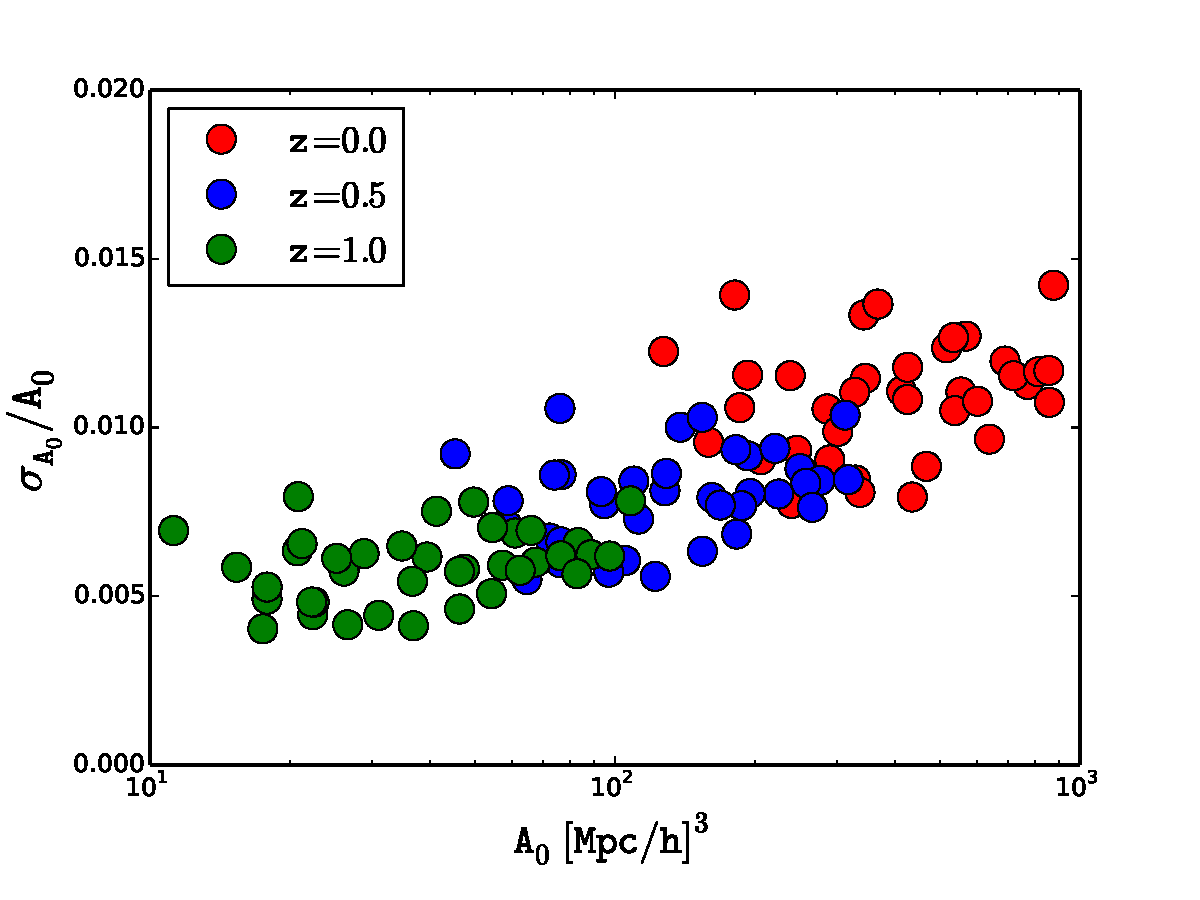
\includegraphics[width=0.48\linewidth]{figures/p2-figures/var_A_0.pdf}
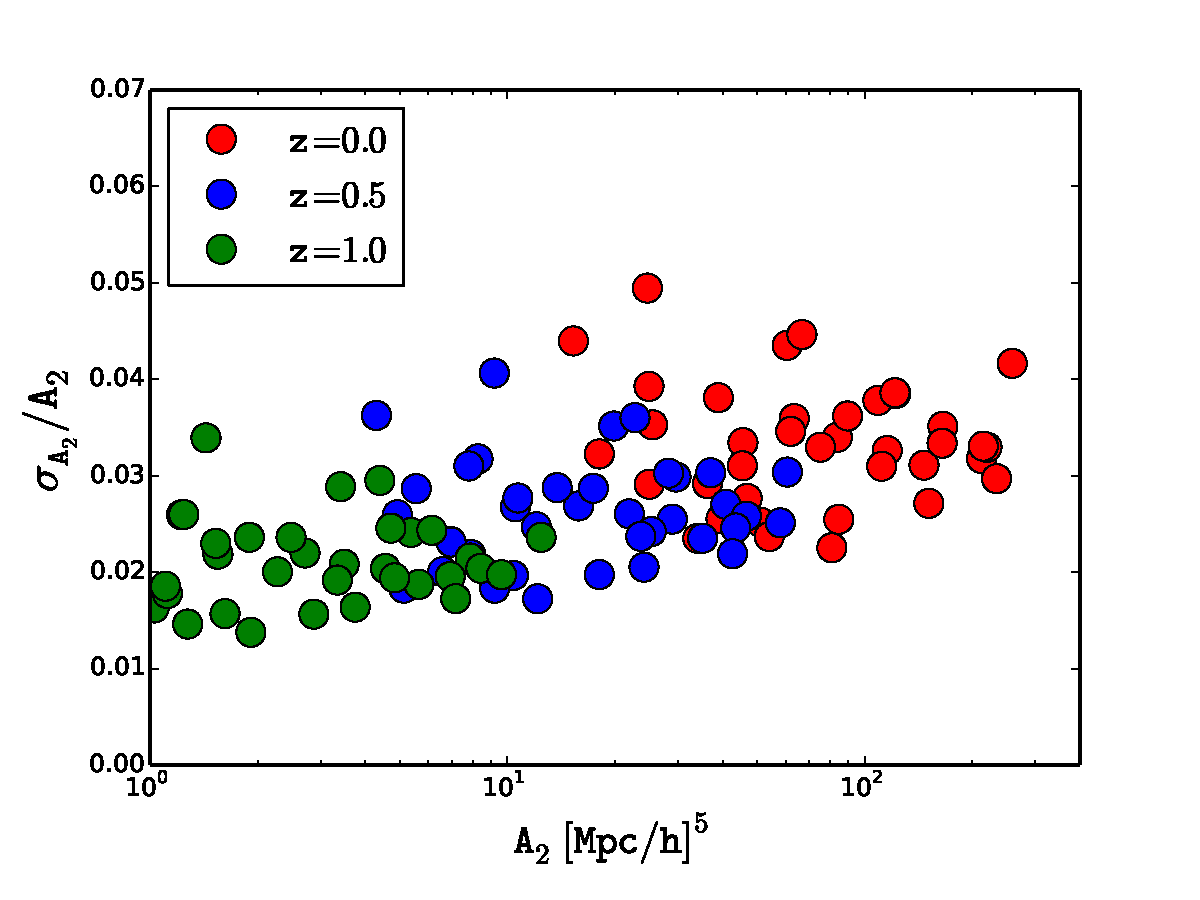
\includegraphics[width=0.48\linewidth]{figures/p2-figures/var_A_2.pdf}
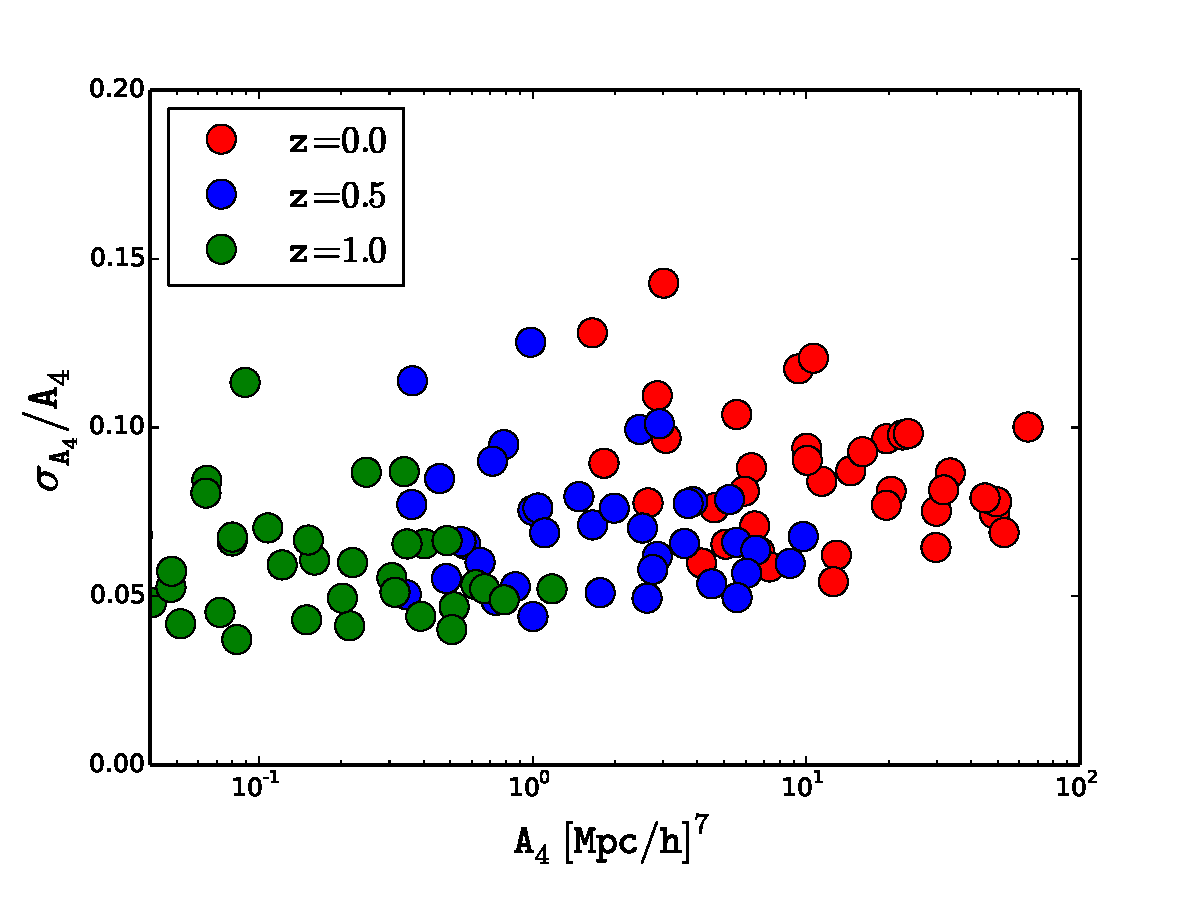
\includegraphics[width=0.48\linewidth]{figures/p2-figures/var_A_4.pdf}
\caption{Relative variance $\Delta A_{2n}/A_{2n}$ versus $A_n$ based on our model for
$A_0$, $A_2$ and $A_4$ for three different redshift: 0.0 (red), 0.5 (blue) and 1.0 (green). Each circle bullet is one cosmological realization of the 38 cosmic emulator nodes.}
\label{p2:fig:variance}
\end{figure}

\clearpage

\begin{equation}
\begin{array}{lcl} 
A_0 & = & \int d\nu f(\nu) \dfrac{M}{\bar{\rho}}\ \Im_0\Im_0 \\ 
\\
A_2 & = & \int d\nu f(\nu) \dfrac{M}{\bar{\rho}}\ 2\Im_0\Im_1 \\ 
\\
A_4 & = & \int d\nu f(\nu) \dfrac{M}{\bar{\rho}}\ (\Im_1\Im_1 + 2\Im_0 \Im_2)
\end{array}
\label{p2:A024}
\end{equation}
\\
with covariance,
\\
\begin{equation}
\resizebox{\linewidth}{!}{$\displaystyle
\mathtt{Cov}(A_iA_j) = 
 \begin{pmatrix}
  \int d\nu\ g(\nu)\ (\Im_0\Im_0)^2
  & \int d\nu\ g(\nu)\ (\Im_0\Im_0) (2\Im_0\Im_1)
  & \int d\nu\ g(\nu)\ (\Im_0\Im_0) (\Im_1\Im_1 + 2\Im_0 \Im_2)\\


  \int d\nu\ g(\nu)\ (\Im_0\Im_0) (2\Im_0\Im_1) 
  & \int d\nu\ g(\nu)\ (2\Im_0\Im_1)^2
  &  \int d\nu\ g(\nu)\ (2\Im_0\Im_1) (\Im_1\Im_1 + 2\Im_0 \Im_2)\\


  \int d\nu\ g(\nu)\ (\Im_0\Im_0) (\Im_1\Im_1 + 2\Im_0 \Im_2)
  & \int d\nu\ g(\nu)\ (2\Im_0\Im_1) (\Im_1\Im_1 + 2\Im_0 \Im_2)
  &  \int d\nu\ g(\nu)\ (\Im_1\Im_1 + 2\Im_0 \Im_2)^2
 \end{pmatrix}
 $}
 \label{p2:eqn:covariance}
\end{equation}
where $i,j=0,2,4$ and
\\
\begin{equation}
	g(\nu) = \dfrac{1}{\mathtt{Volume}} f(\nu) \left(\dfrac{M}{\bar{\rho}}\  \right)^3
\end{equation}



In this paper we terminate this series after $A_4$ term. One can always go to higher order terms to get desired accuracy at higher $k$.

We will present the results of analytic calculations of $A_{2n}$ in the next section. 
Calculating the variance of each of these coefficients is as straightforward as calculating the coefficient itself, 
performing the integrals over the halo mass function. We calculate the variance on these terms for a volume of $1\ ({\rm 
Gpc}/h)^3$ for different cosmological models 
(the 38 models explained in next section) at three different redshifts: 0.0, 0.5 and 1.0. Figure \ref{p2:fig:variance} shows the relative variance of the three coefficients. We find 
for 1\ ${\rm (Gpc)/h}^3$ the relative error $\sigma_{A_0}/A_0$ varies from 0.5 to 2 \%,
whereas on $\sigma_{A_2}/A_2$ and $\sigma_{A_4}/A_4$  vary from $1\%\ \rm{to}\ 7\%$ and from $2\%\ \rm{to}\ 20\%$, respectively, depending on the cosmology and redshift. 
We see that the relative error on $A_{2n}$ increases with $n$: this is a consequence of the fact that terms with higher 
$n$ receiving a larger contribution from higher mass objects, since the mass scaling of the 
integrand for $A_{2n}$ in the equations above is $M^{1+2n/3}$, while for the variance it is $M^{3+4n/3}$.
Higher mass objects are rarer and their Poisson fluctuations are larger, hence the relative 
variance is increased. 
Below we will compute the sensitivity of these parameters to cosmology: we will show that $A_0$ contains 
most of the information on the amplitude $\sigma_8$. 
In this paper we use halo mass function of \cite{2008ApJ...688..709T}. 

So far we assumed $F(k)=1$ without specifying its role. 
It was pointed out already in the original halo model \citep{2000MNRAS.318..203S} 
that the 1-halo term of the halo model fails to account for mass 
and momentum conservation at low $k$: the nonlinear corrections to the power spectrum have to scale as 
$k^4$ or $-k^2P(k)$ at low $k$, while the leading order of the 1-halo term scales as $k^0$. 
At very low $k$ such a term may even dominate over the linear term, which cannot be physical in 
the context of dark matter, even though it can happen in the context of galaxies \cite{2013PhRvD..88h3507B}. 
We will impose this constraint by simply fitting the residuals to the simulations at low $k$ and apply the derived transfer 
function $F(k)$, which vanished at low $k$,
to the model. We will show that the function $F(k)$ does not strongly depend on the cosmological 
model and we will thus ignore its dependence on cosmological parameters. 

%========================================================================================

\section{Calibrating the model with simulations}
\label{p2:sec:calibration}

We use cosmic emulator (\cite{2010ApJ...715..104H,2009ApJ...705..156H,2010ApJ...713.1322L}) to evaluate the power spectra for 
each of the 38 emulator simulations and assume in each case it gives the true non-linear matter power spectrum. These reference power spectra are correct to nearly 1$\%$ up to $k\sim 1\ h \rm{Mpc}^{-1}$ at 38 different nodes (labelled as 0 to 37) in cosmological parameter space. This accuracy degrades to $5\%$ when computing the power spectrum away from the 
nodes.  Node 0 cosmology is closest to the WMAP-7 cosmology and we use it as a reference cosmology. 
We fit these simulation
power spectra with our description -- Quasi-linear Zeldovich term plus modified 1-halo term as a 
sum of even powers of $k$, to determine coefficients $A_{2n}$ as a function of cosmology.

%----------------------------------------------

\begin{figure}[p]
\centering
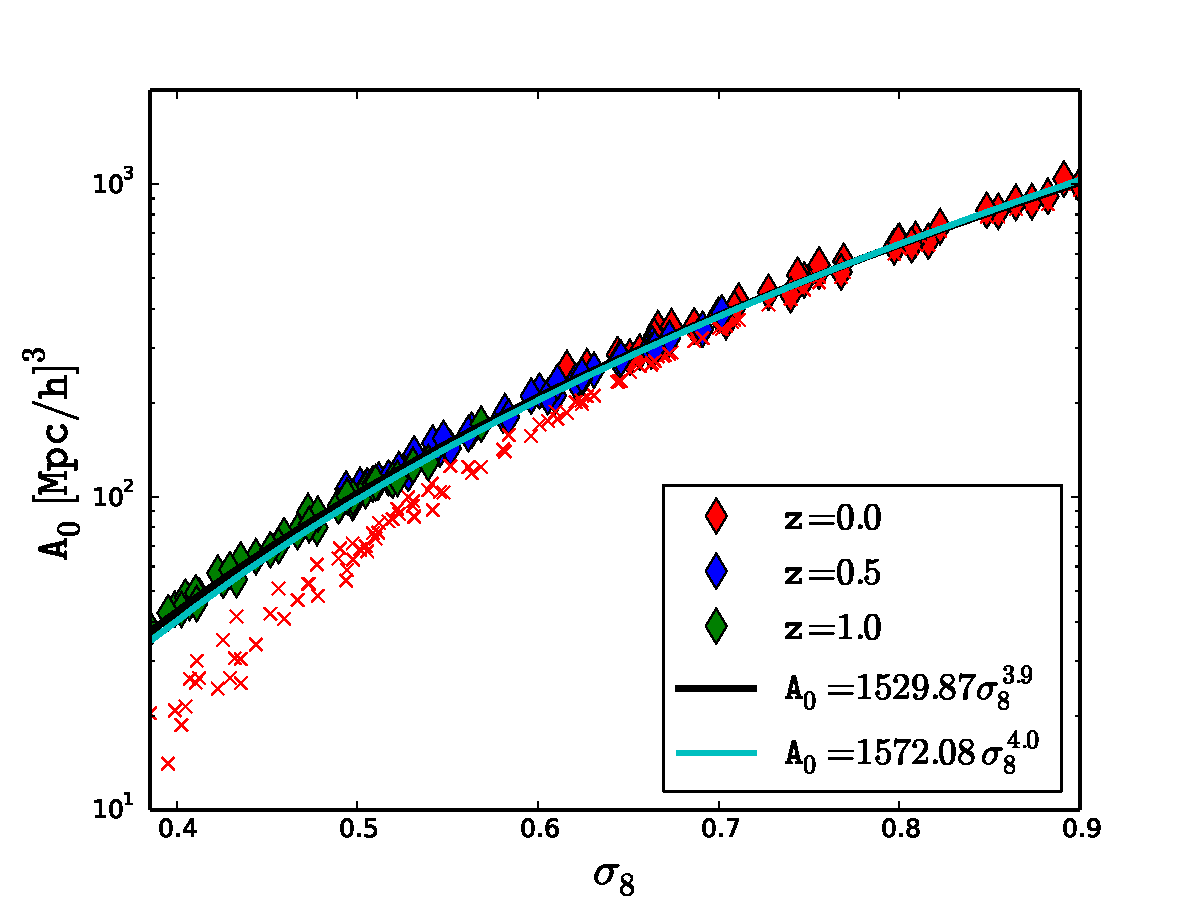
\includegraphics[width=0.45\linewidth]{figures/p2-figures/A0_s8.pdf}
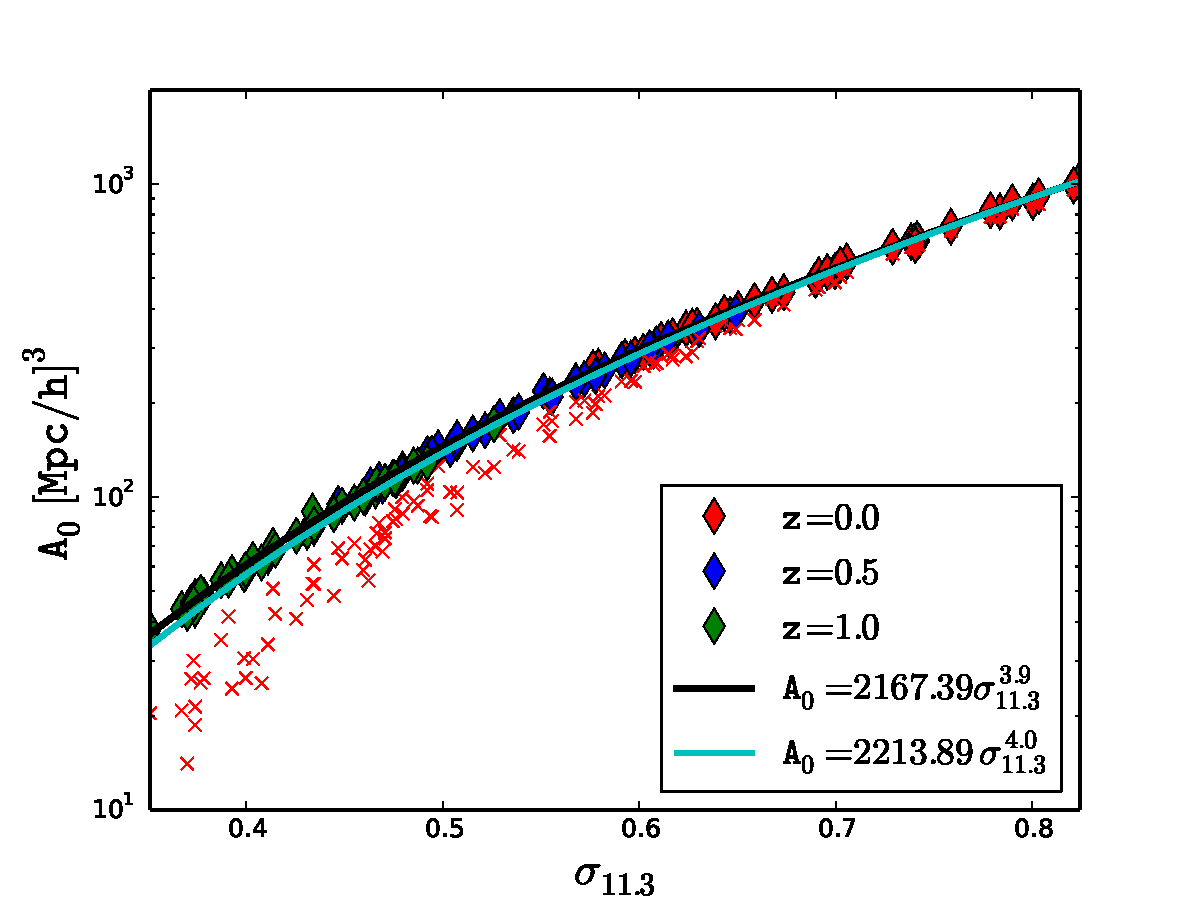
\includegraphics[width=0.45\linewidth]{figures/p2-figures/A0_s113.pdf}
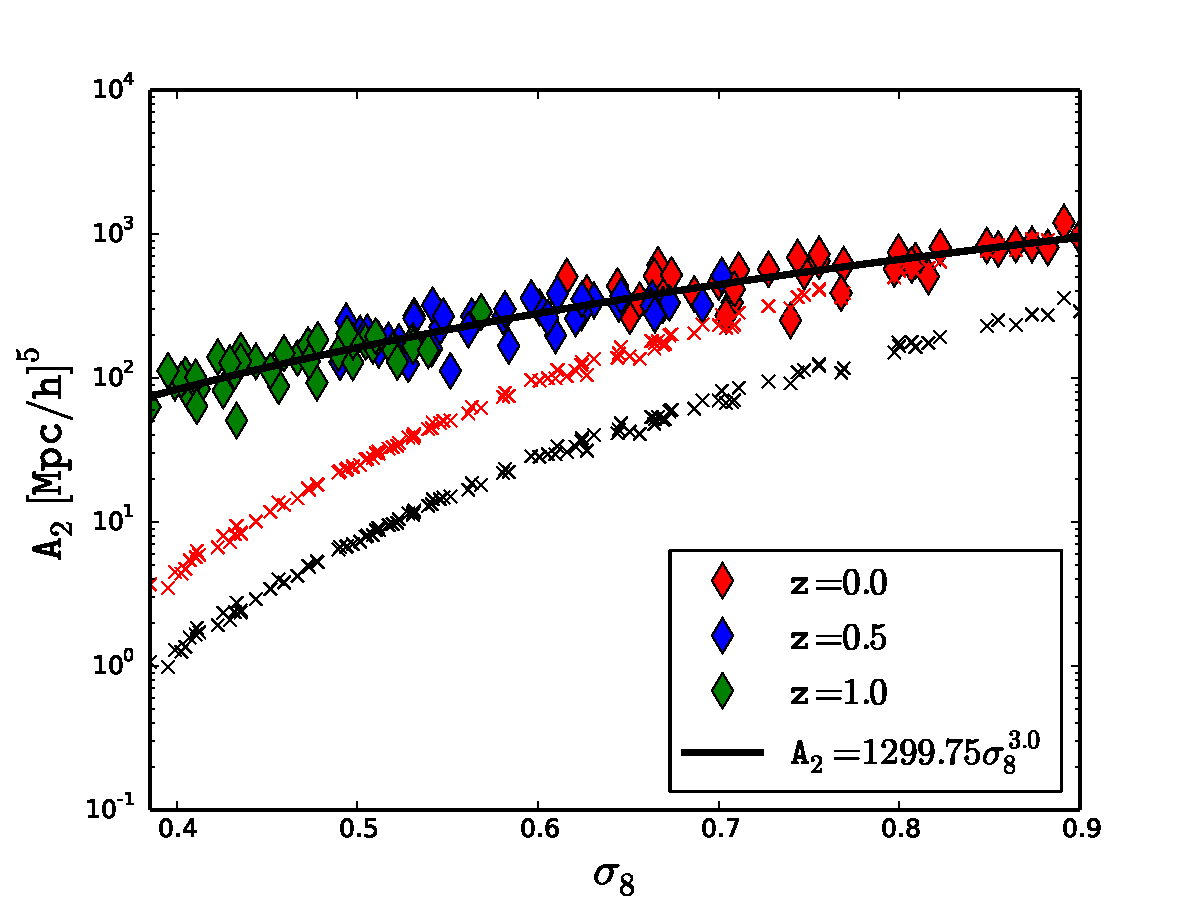
\includegraphics[width=0.45\linewidth]{figures/p2-figures/A2_s8.pdf}
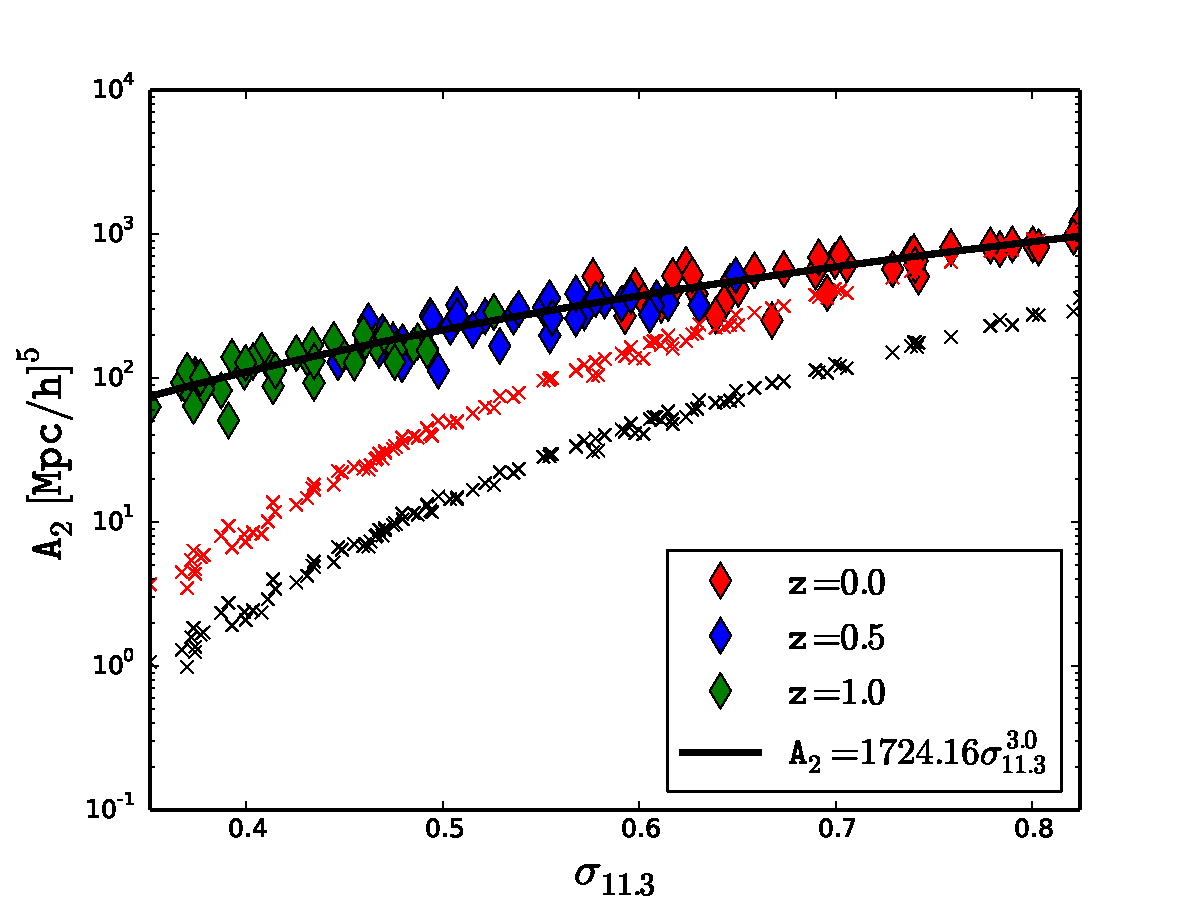
\includegraphics[width=0.45\linewidth]{figures/p2-figures/A2_s113.pdf}
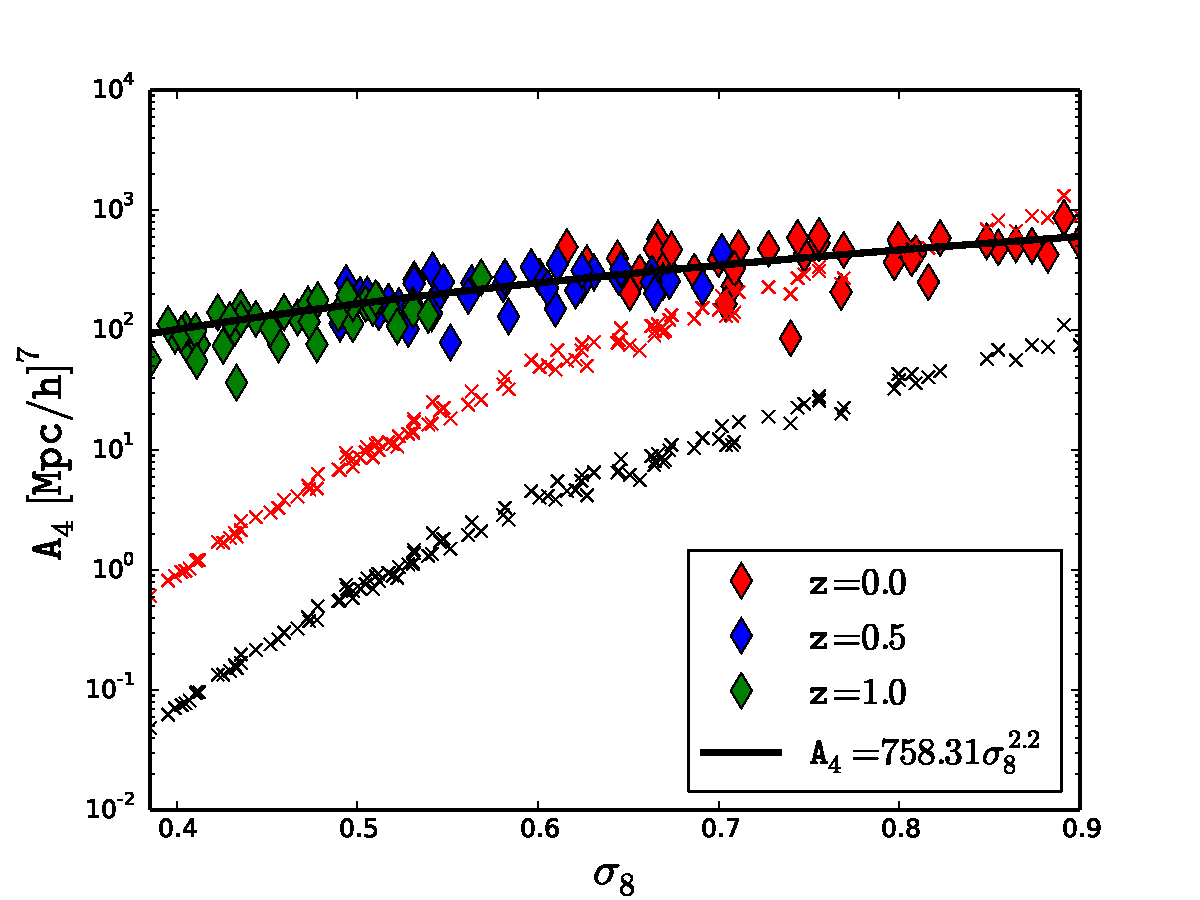
\includegraphics[width=0.45\linewidth]{figures/p2-figures/A4_s8.pdf}
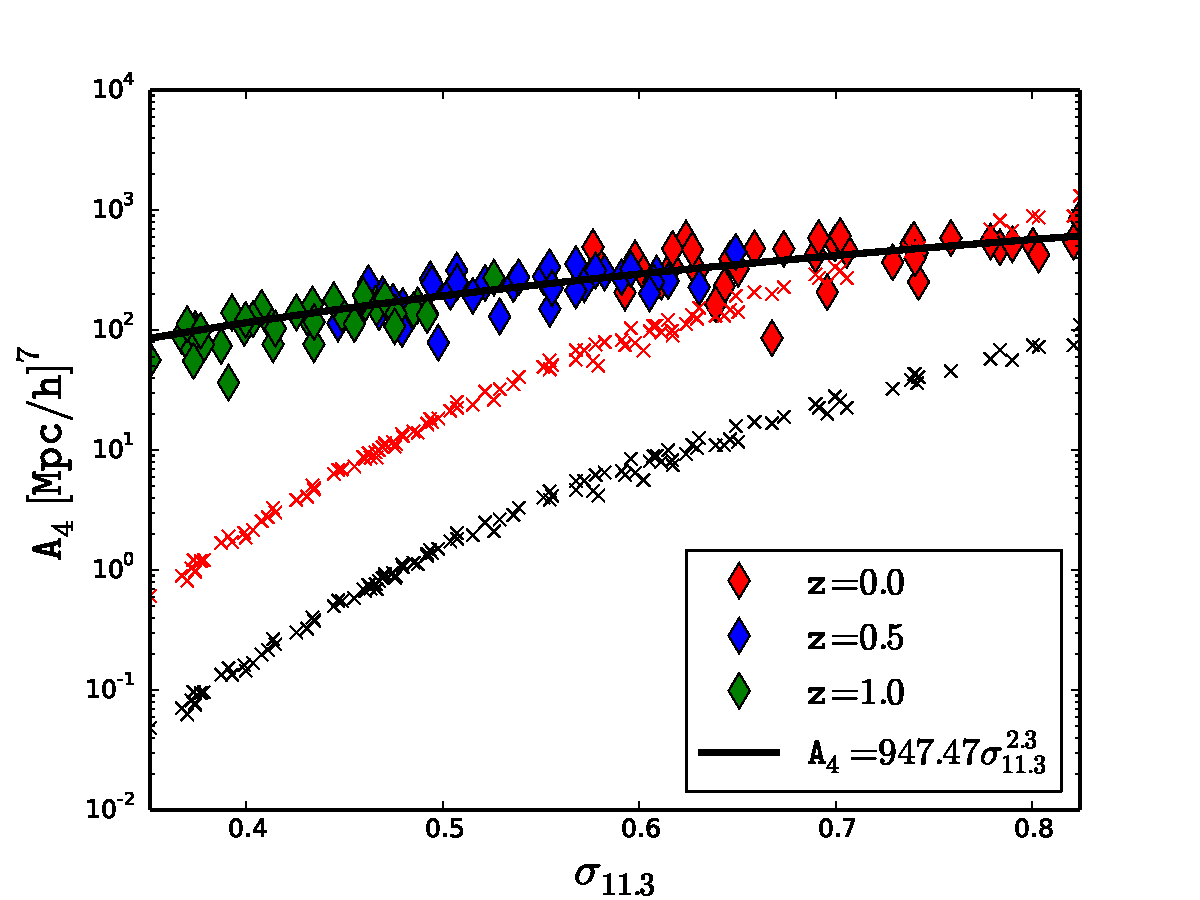
\includegraphics[width=0.45\linewidth]{figures/p2-figures/A4_s113.pdf}
\caption[Fitted coefficients versus fluctuation amplitudes]{Fitted coefficients $A_0,\, A_2 \ \& \ A_4$ versus $\sigma_8$ (Left column) and $\sigma_{11.3}$ (Right column). 
We see that $\sigma_{11.3}$ reduces the scatter relative to $\sigma_8$ for $A_0$. Solid black line is the best fit power law stated in the legend. The halo model prediction is shown in crosses, using the usual halo concentration 
parameter $R_s=R_{\rm vir}/c$, with halos extending to the virial radius $R_{\rm vir}$, defined at the mean overdensity of 
200 (black crosses), and doubling that 
to $2R_{\rm vir}$ (red crosses). Halo model agrees well with simulations for $A_0$ 
at late redshifts, 
but not for $A_2$ and $A_4$ both in terms of amplitude and in terms of $\sigma_8$ or $\sigma_{11.3}$ scaling. Extending 
the halo profile to twice the virial radius improves the agreement.}
\label{p2:fig:A_sigma}
\end{figure}

\clearpage

To begin with, we fit the even power-law (equation \ref{p2:eqn:pk1h_powerlaw} with $F(k)=1$) to the difference between matter power spectrum from emulator $\rm{P_{Emu}}$ and the Zeldovich term $\rm{P_{Zel}}$ for all 38 cosmologies and three redshifts: 0.0, 0.5, 1.0 between $k = 0.2$ and $0.8\ h \rm{Mpc}^{-1}$. 

All the coefficients fitted, $A_0, \, A_2 \ \& \ A_4$, are strongly correlated with $\sigma_8$, with 
$A_0$ having the least scatter. Figure \ref{p2:fig:A_sigma} shows the scaling of these coefficients with $\sigma_8(z)$ and $\sigma_{11.3}$(z), where the latter was chosen to minimize the scatter in $A_0$.
Each of these coefficients can be approximately fit as a power law irrespective of the redshift and cosmology,
with $\sigma_8(z)$ scaling
\begin{equation}
 	A_0 \propto \sigma_{8}^{3.9},\ A_2 \propto \sigma_{8}^{3.0},\ A_0 \propto \sigma_{8}^{2.2}.
\label{p2:slopea024}
\end{equation}
It is not straightforward to determine the errors since this is not a formal fit to a set of data points with individual 
errors. In figure \ref{p2:fig:A_sigma} we also show results when the slope of $A_0$ is 4.0: we see this is also a good fit over 
the range. 

Figure \ref{p2:fig:A_sigma} also shows the predictions of the halo model for these coefficients (in black crosses). While the 
halo mode predicts well $A_0$ at low redshifts, it fails for higher order coefficients. This can be improved 
if the virial radius is increased by roughly a factor of 2 at low redshifts, and more than that at higher redshifts
(which needs to be taken to power $2n$ to evaluate the effect on $A_{2n}$), shown as red crosses in figure \ref{p2:fig:A_sigma}. The failure of the halo model to quantitatively 
predict these coefficients is not surprising: the halos do not suddenly stop at the virial radius and the halo model has 
some flexibility in how it is implemented. Our goal here is not to understand the halo model, but to have accurate 
predictions.  For this reason we will just use the fits of $A_{2n}$ coefficients to simulations in this paper. 

The next step is to correct for the scatter around the best fit $\sigma_{8}$. A correlation is noticed between the residual of the coefficients with the effective slope $n_{\rm eff}$. This is shown in figure \ref{p2:fig:ns_res}. Here the residual means the difference between the diamond-bullets and best fit lines in figure \ref{p2:fig:A_sigma} and 
effective slope $n_{\rm eff}$ 
is calculated as the slope of the linear matter power spectrum at $k \sim 0.2\ h \rm{Mpc}^{-1}$. The higher order coefficients have larger 
scatter and stronger correlation between this residual and effective slope. We tested the scalings for 
few different values of $R$ in $\sigma_R$ and found minimum scatter for $\sigma_{11.3}$, 
which can be seen in figures \ref{p2:fig:A_sigma} and \ref{p2:fig:ns_res}. By using $\sigma_{11.3}$ instead of $\sigma_8$ one can remove the correlation with effective slope for $A_0$, so no $n_{\rm eff}$ correction is needed for $A_0$. However, $A_2 \ \& \ A_4$ 
still need to be corrected for this correlation, although
the correction is smaller in case of $\sigma_{11.3}$ than $\sigma_8$. Hence the corrected expressions for these coefficients are
\begin{equation}
	A_0 = 1529.87 \sigma_8^{3.9} \times (1 + [-0.22 n_{\rm{eff}} - 0.4]),\ \rm{or}\ 
	A_0 = 2167.39 \sigma_{11.3}^{3.9},
	\label{p2:eqn:a0}
\end{equation}
\begin{equation}
	A_2 = 1299.75 \sigma_8^{3.0} \times (1 + [-1.58 n_{\rm{eff}} - 2.8]),\ \rm{or}\ 
	A_2 = 1724.16 \sigma_{11.3}^{3.0} \times (1 + [-1.39 n_{\rm{eff}} - 2.5])
	\label{p2:eqn:a2}
\end{equation}
\begin{equation}
	A_4 = 758.31 \sigma_8^{2.2} \times (1 + [-2.27 n_{\rm{eff}} - 4.2]),\ \rm{or}\ 
	A_4 = 947.47 \sigma_{11.3}^{2.3} \times (1 + [-2.12 n_{\rm{eff}} - 3.9])
	\label{p2:eqn:a4}
\end{equation}

\begin{figure}[p]
\centering
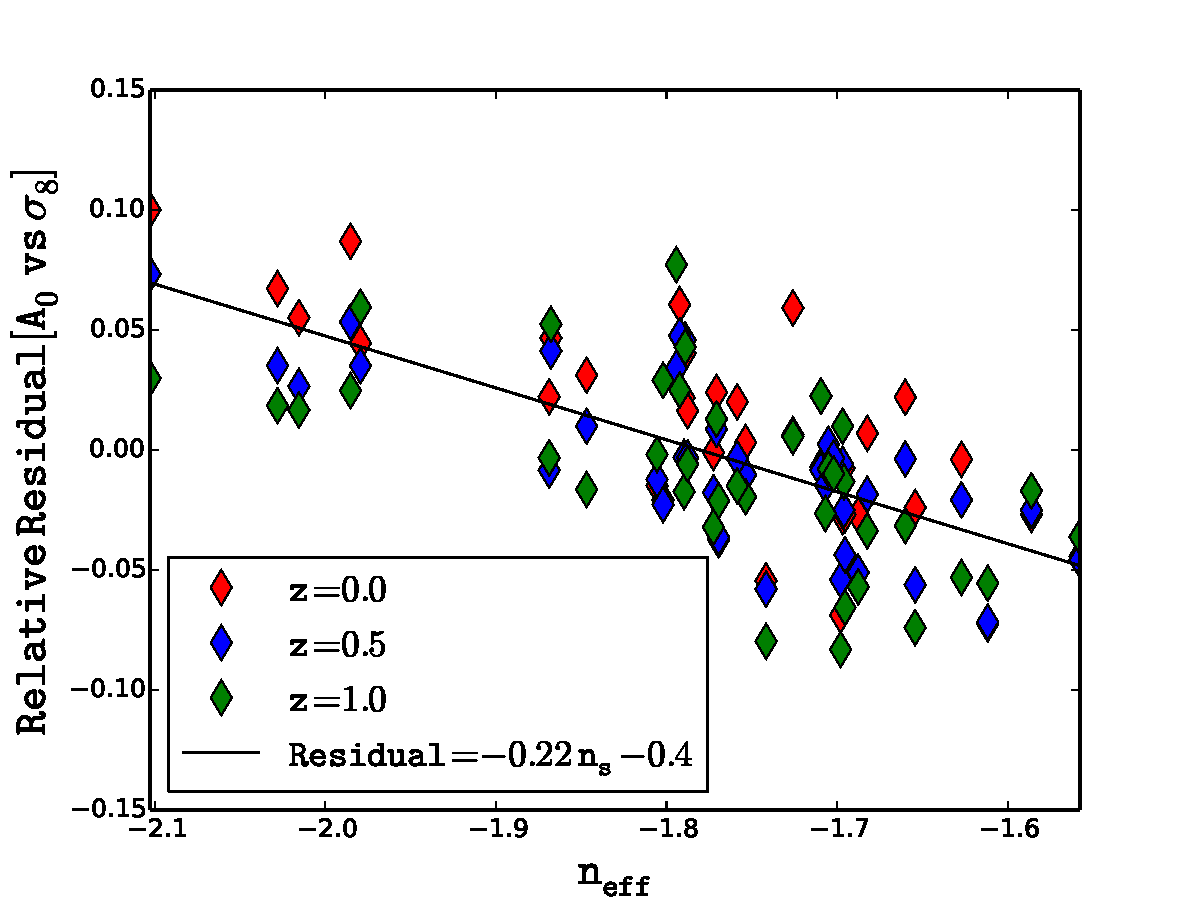
\includegraphics[width=0.48\linewidth]{figures/p2-figures/ns_residueA0rel_kfixed_sigma8.pdf}
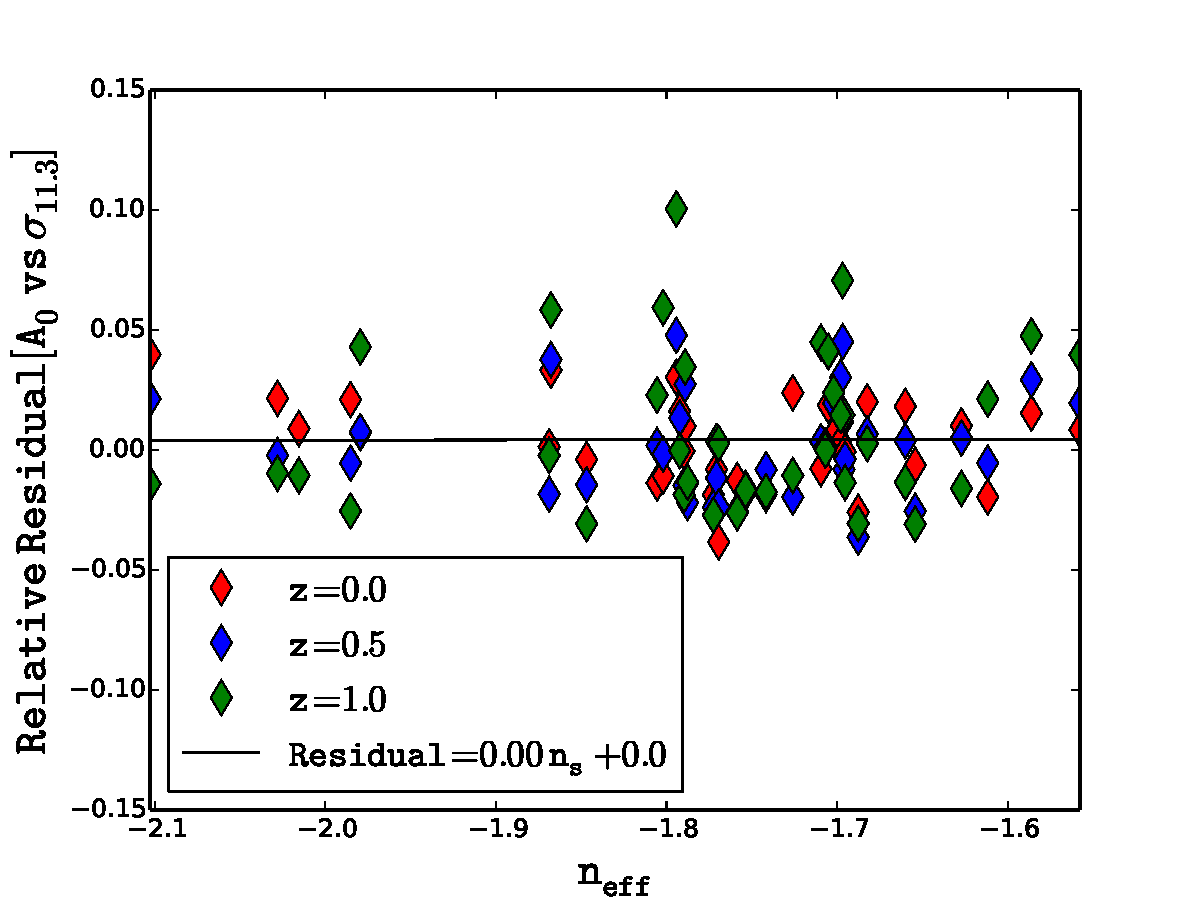
\includegraphics[width=0.48\linewidth]{figures/p2-figures/ns_residueA0rel_kfixed_sigma11.3.pdf}
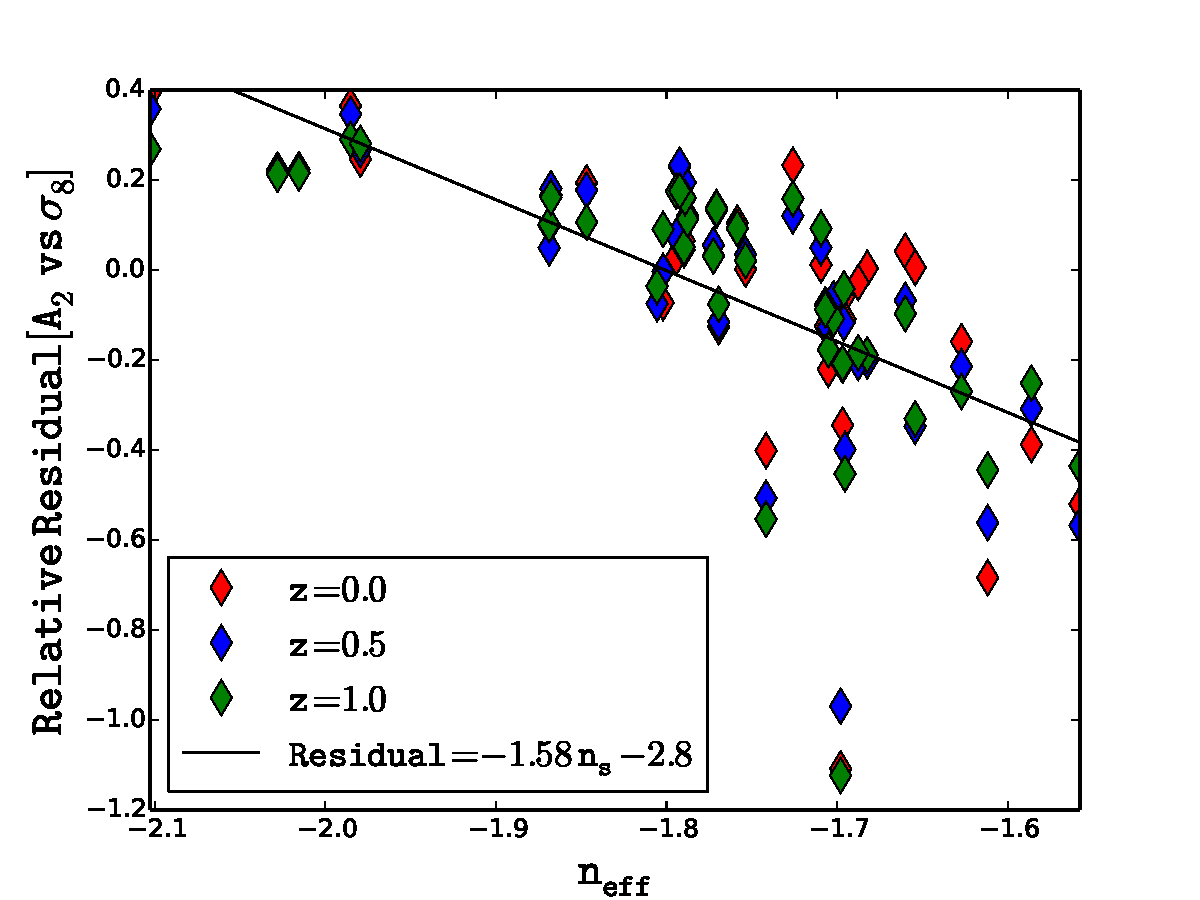
\includegraphics[width=0.48\linewidth]{figures/p2-figures/ns_residueA2rel_kfixed_sigma8.pdf}
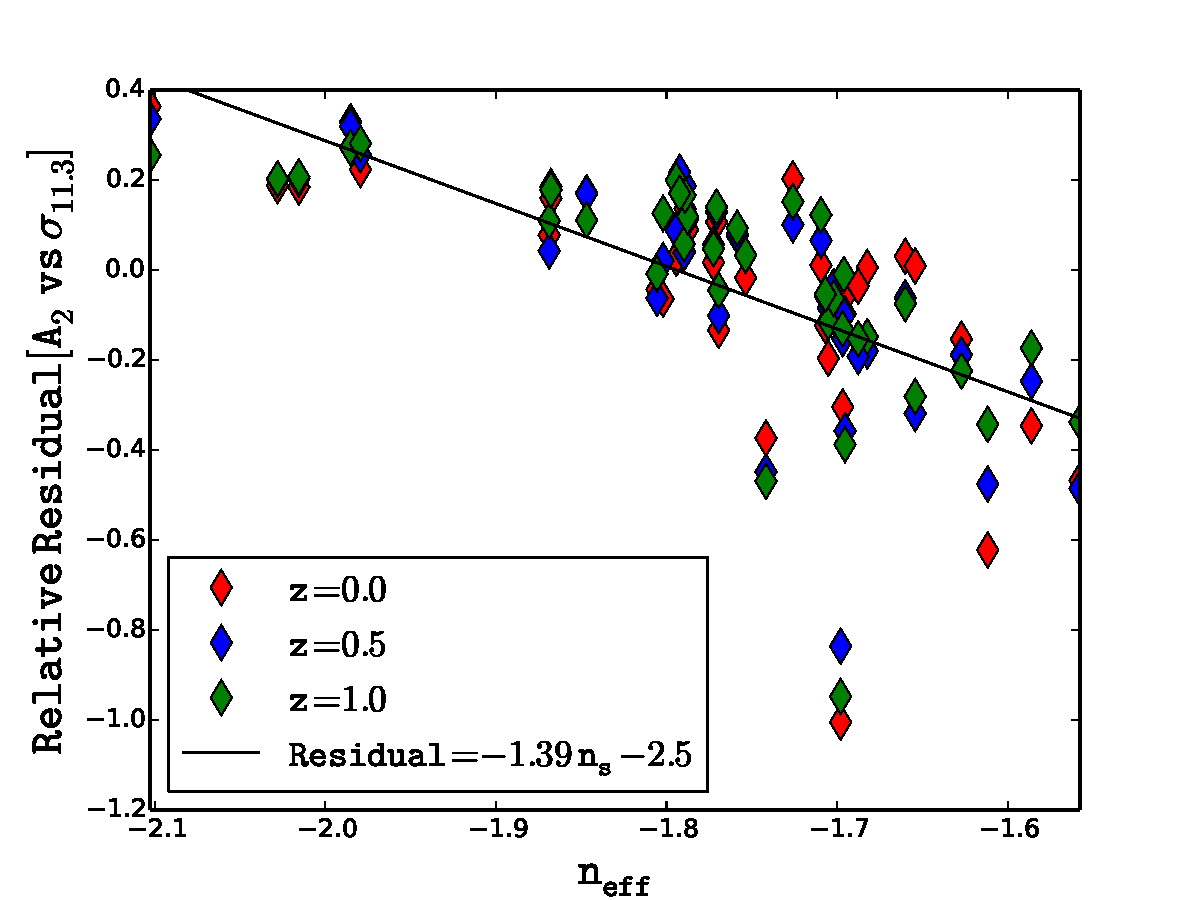
\includegraphics[width=0.48\linewidth]{figures/p2-figures/ns_residueA2rel_kfixed_sigma11.3.pdf}
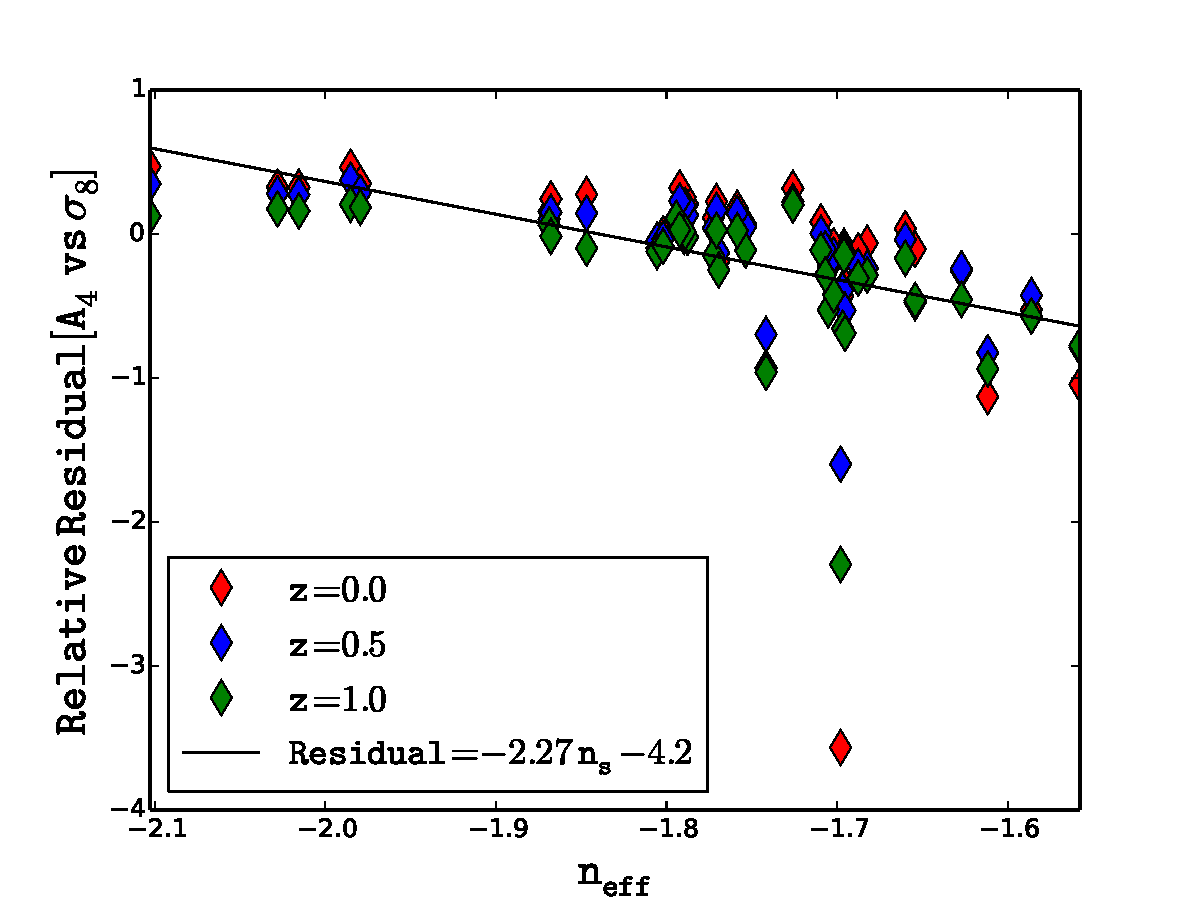
\includegraphics[width=0.48\linewidth]{figures/p2-figures/ns_residueA4rel_kfixed_sigma8.pdf}
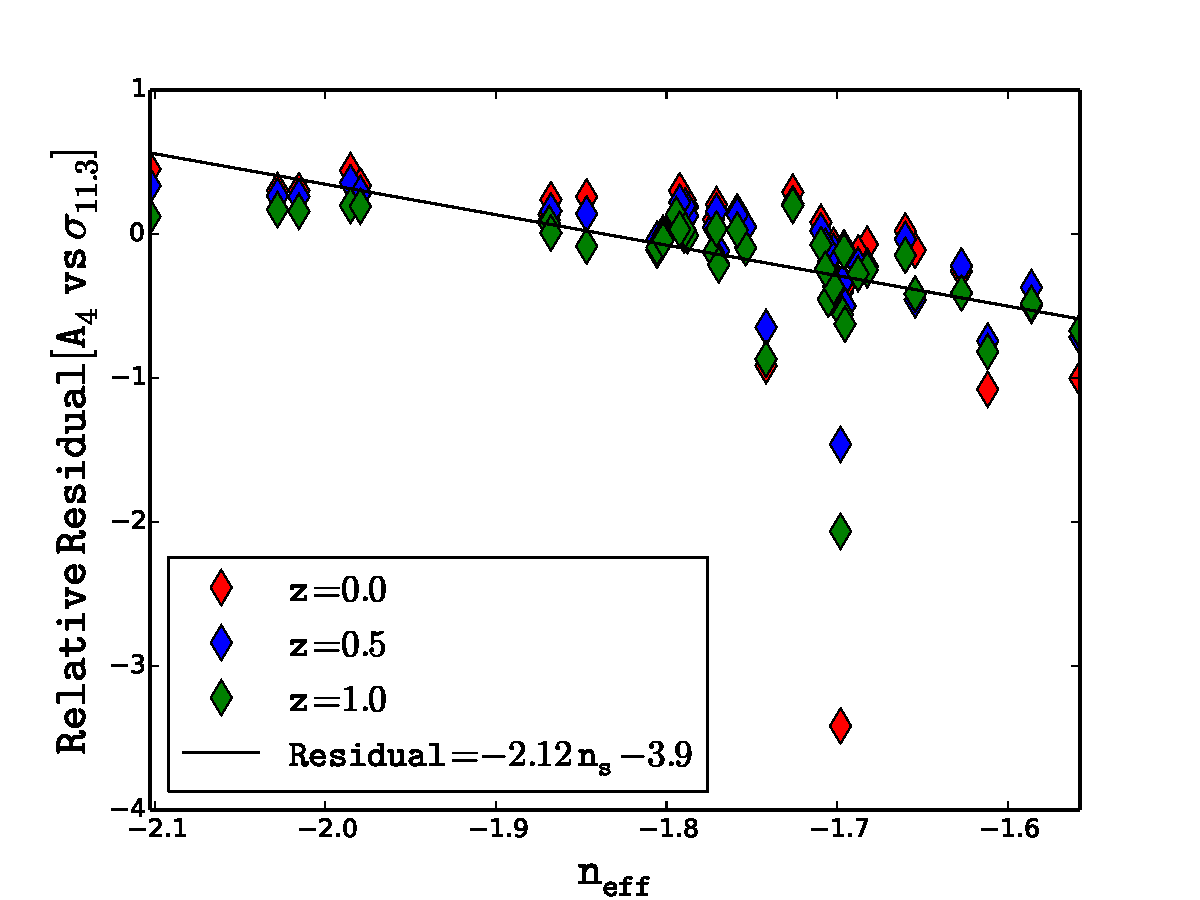
\includegraphics[width=0.48\linewidth]{figures/p2-figures/ns_residueA4rel_kfixed_sigma11.3.pdf}

\caption[Effective-slope correlations after amplitude scaling]{Correlation between effective slope ($n_{\rm eff}$) and 
residuals after $\sigma_8$ (Left column) or $\sigma_{11.3}$ (Right column) scaling is taken out 
and their respective best fit. Solid black line is the best linear fit as stated in the legend.}
\label{p2:fig:ns_res}
\end{figure}

\clearpage
%----------------------------------------------

We still need to account for the mass conservation, which forces the 1-halo term to go to 0 at low $k$. 
In figure \ref{p2:fig:bestfit}, we plot the ratio of the difference between $\rm{P_{Emu}}$ and $\rm{P_{Zel}}$ with $\rm{P_{SimFit}}$ which is given by
	$\rm{P_{SimFit}} = A_0 - A_2k^2 + A_4 k^4$, 
where, these coefficients are the best fit values to $(\rm{P_{emu} - P_{Zel}})$ for all 38 cosmologies (Diamond bullets in figure \ref{p2:fig:A_sigma}). The top-left, top-right and bottom-left panel shows the same quantity at three different redshifts: 0.0, 0.5 and 1.0 respectively. All 38 curves in each panel are very close to 1 for $k$ between 0.2 and $0.8 \ h \rm{Mpc}^{-1}$, which is expected as these coefficients are fitted in that range in the first place. Outside this range the scatter increases. We took the average of all these 38 curves at all three redshifts and fit it to a $10^{th}$ 
order polynomial, requiring to vanish at low $k$. 
The bold solid black line and dashed red curve represents the average and best fit to the average, respectively. 
It can be seen in bottom-right panel of figure \ref{p2:fig:bestfit} that these best fit to the average are very close to node 0 cosmology curve and also very close to each other for different redshifts for $k<0.8 \ h \rm{Mpc}^{-1}$. 
We average of these three best-fit curves, at three different redshifts, to build the function $F(k)$ for the 1 halo term, 
which we model as
\begin{equation}
	F(k) = \sum_{n=0}^{10} a_n k^n, 
\label{p2:eqn:fk}
\end{equation}
where the coefficients $a_n$ are listed in table \ref{p2:tbl:an}. 
As expected by the mass conservation arguments, and seen in figure \ref{p2:fig:bestfit},
this correction drops to zero for $k<0.1\ h \rm{Mpc}^{-1}$. 
In principle we should force it to go to 0 as $k^2$, but we found this caused problems to 
the fit at higher $k$: the effects of $F(k)$ are very small in any case and in most instances below 1\%, since
at low $k$ the Zeldovich term dominates. 
For this reason we will assume this correction is 
independent of the cosmological model or redshift. 

\begin{table}[p]
\begin{center}
\resizebox{\linewidth}{!}{%
\begin{tabular}{|cccccccccccc|}
\hline
\hline
 $a_n$ & $a_0$ & $a_1$& $a_2$& $a_3$& $a_4$& $a_5$& $a_6$& $a_7$& $a_8$& $a_9$& $a_{10}$ \\
\hline
value &0.0 & 21.814& -174.134& 747.369 & -2006.792 & 3588.808 & -4316.241 & 3415.525 & -1692.839 & 474.377 & -57.228\\
\hline
\hline
\end{tabular}%
}
\caption{Coefficients to calculate the correction function, equation \ref{p2:eqn:fk}.
The units of the coefficient $a_n$ is $(\rm{Mpc}/h)^n$.}
\label{p2:tbl:an}
\end{center}
\end{table}

\clearpage

\begin{figure}[p]
\centering
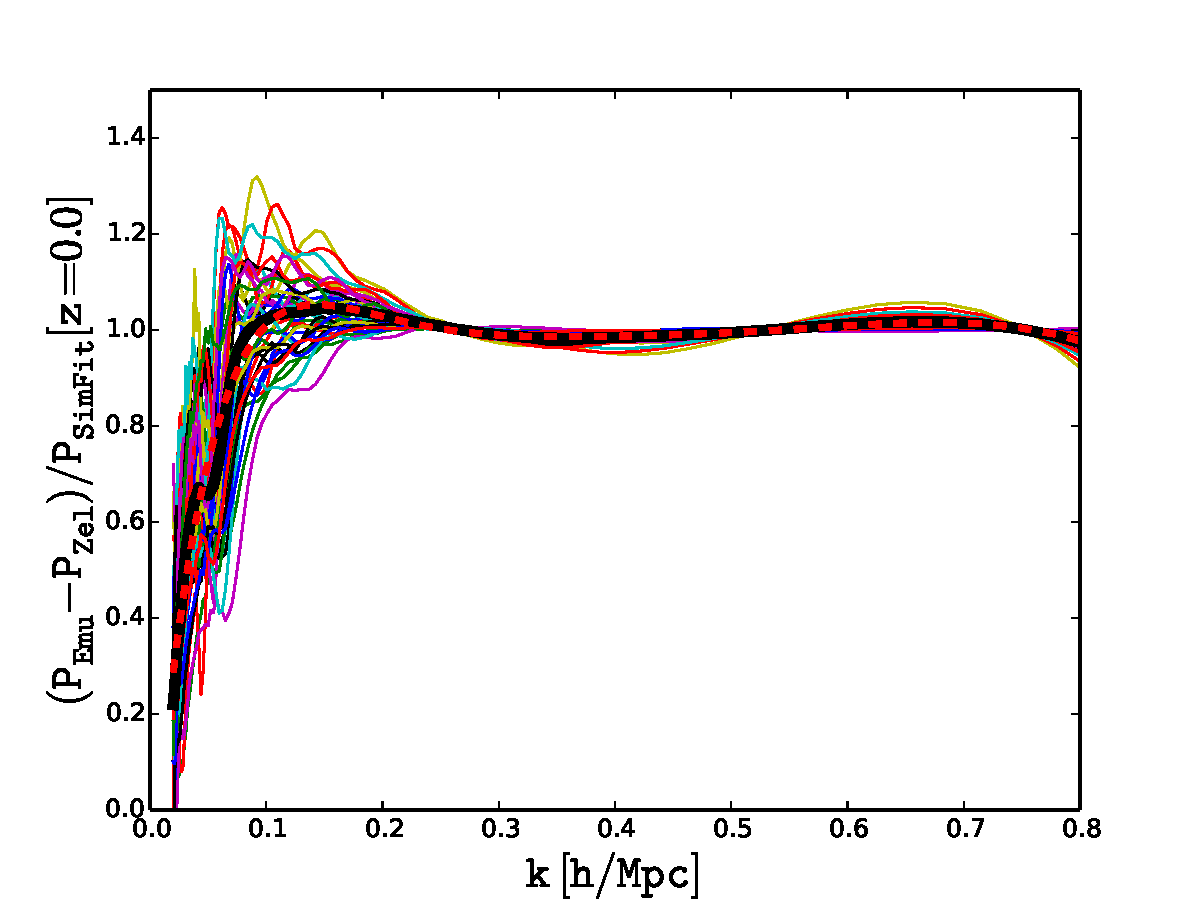
\includegraphics[width=0.48\linewidth]{figures/p2-figures/pk_emu_zel_vs_psim_z0.0_k0.2_0.8_nscorrection.pdf}
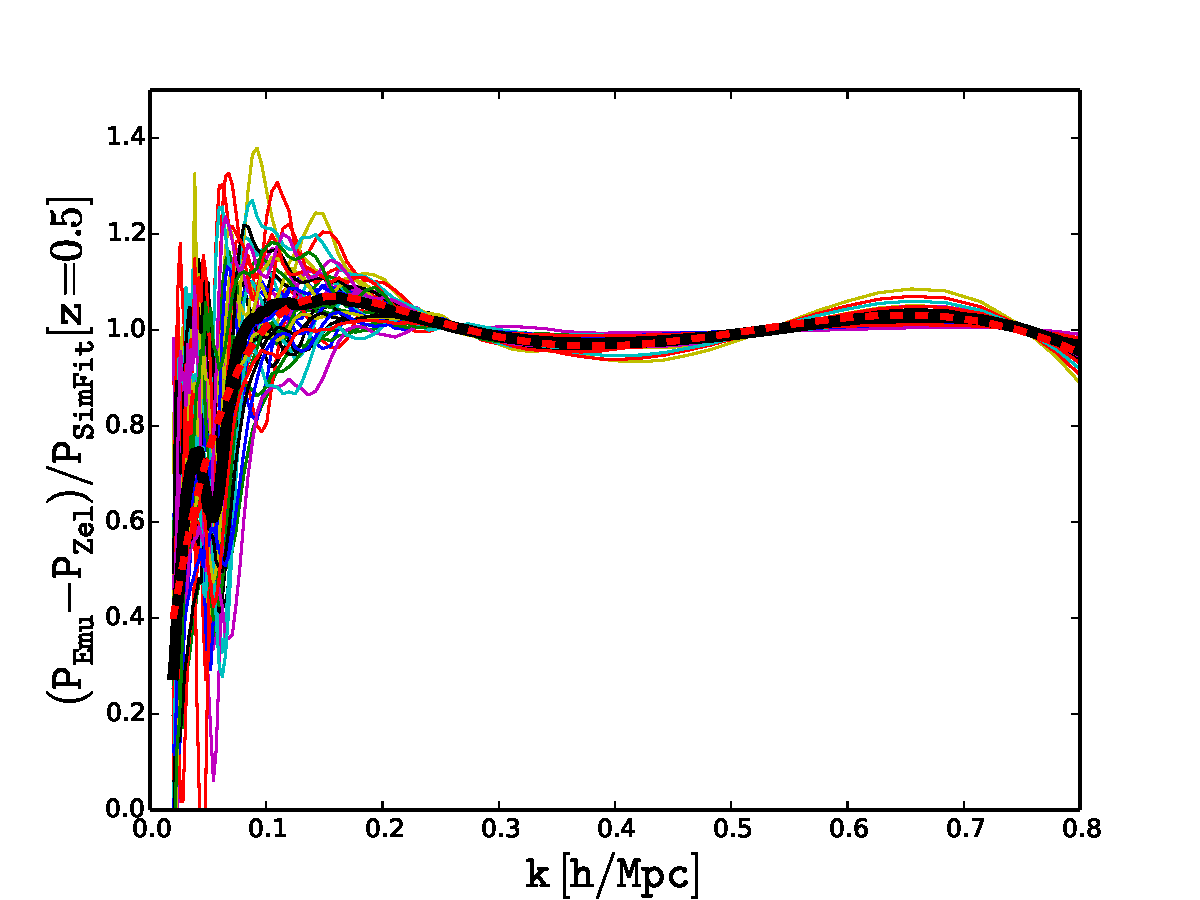
\includegraphics[width=0.48\linewidth]{figures/p2-figures/pk_emu_zel_vs_psim_z0.5_k0.2_0.8_nscorrection.pdf}
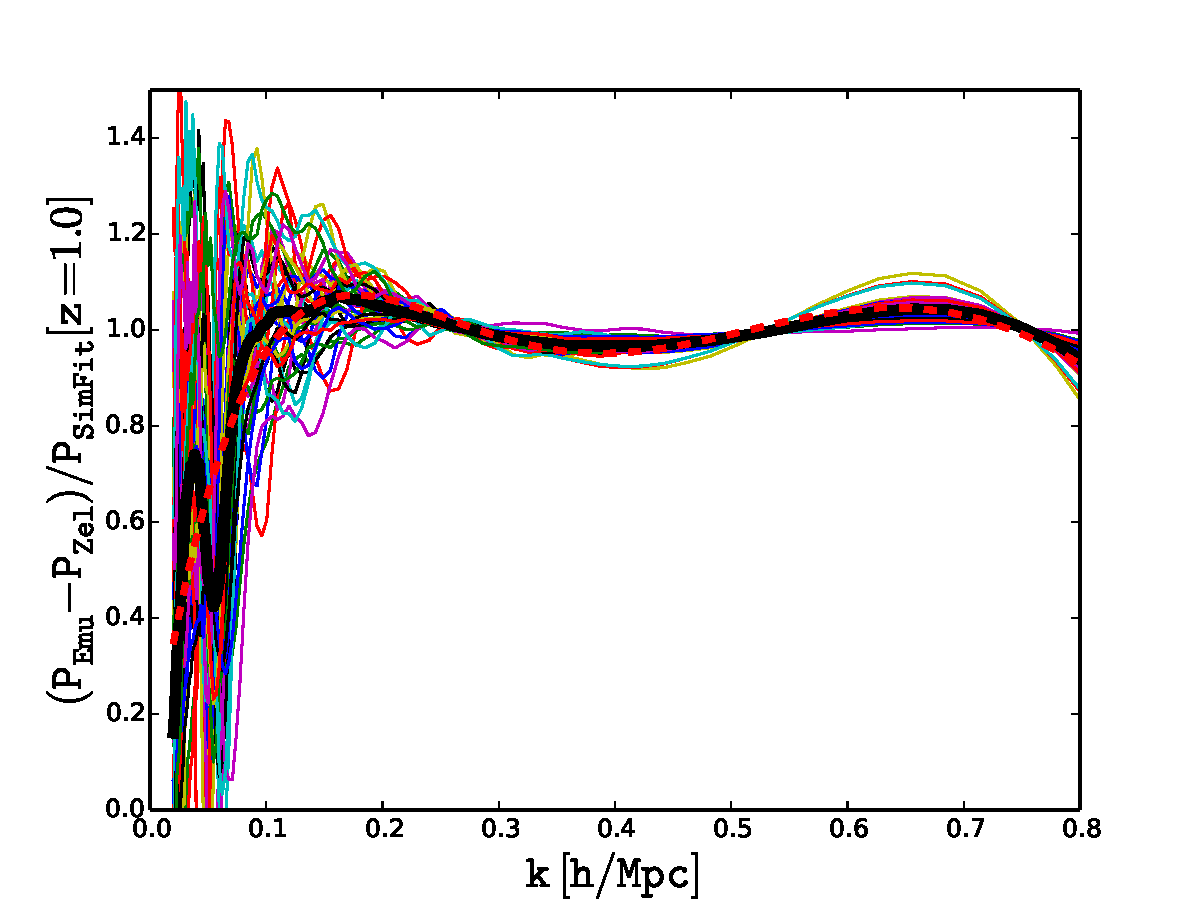
\includegraphics[width=0.48\linewidth]{figures/p2-figures/pk_emu_zel_vs_psim_z1.0_k0.2_0.8_nscorrection.pdf}
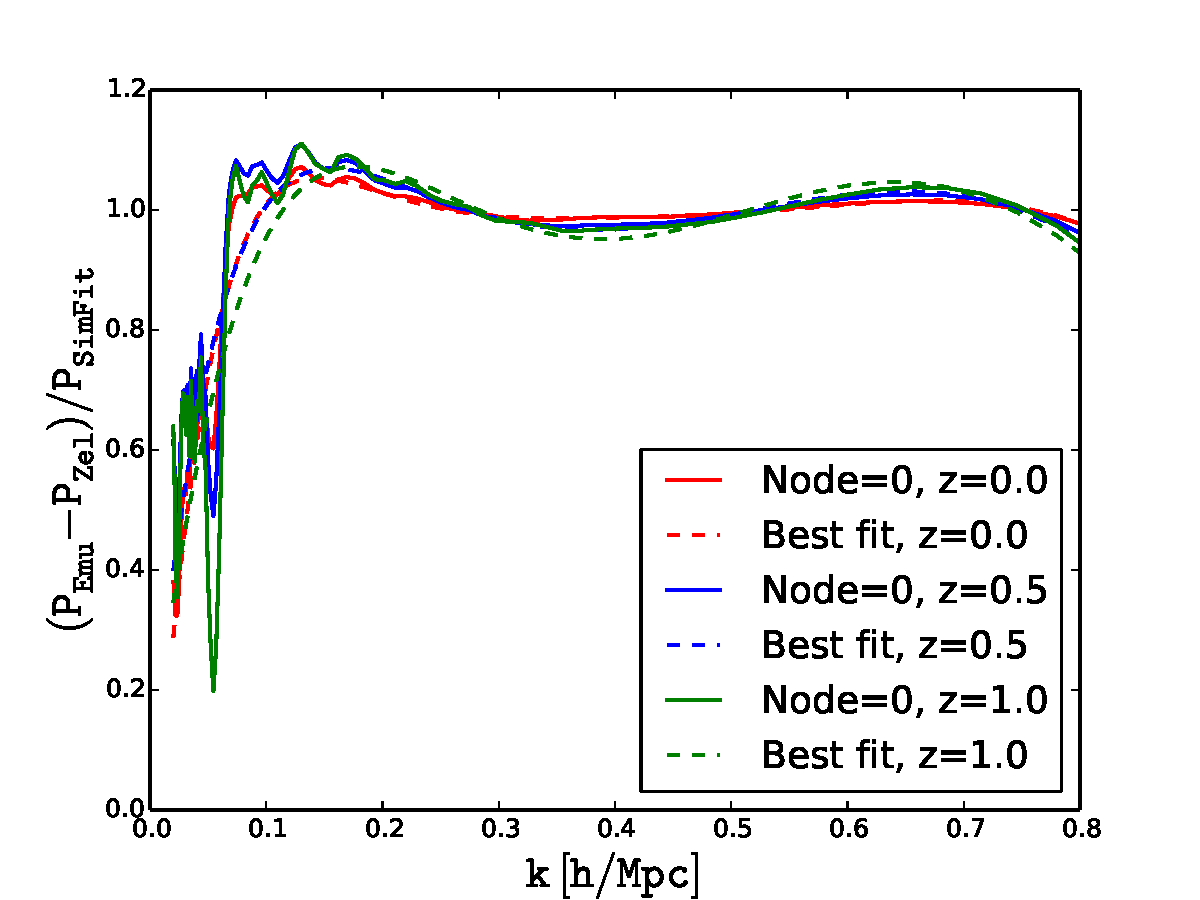
\includegraphics[width=0.48\linewidth]{figures/p2-figures/node0_bestfit.pdf}

\caption{The first three panel (in reading order), shows the ratio of $(\rm{P_{emu} - P_{Zel}})$ and $\rm{P_{SimFit}} = A_0-A_2k^2+A_4k^4$, where the coefficients $A_0, A_2, A_4$ are the best fit coefficients to the emulator matter power spectrum for all 38 cosmological models (in different colors) at three different redshifts: 0.0 (top-left), 0.5 (top-right) and 1.0 (bottom-left). Bottom-right panel shows same quantity for node 0 and the best fit to the average (of 38 coloured curves in first three panels) at three different redshifts.}
\label{p2:fig:bestfit}
\end{figure}

\clearpage

We combine the above two terms to obtain the matter power spectrum as:

\begin{equation}
	P(k,z) = P_{\rm zel}(k,z) + P_{\rm 1h}(k,z)
	\label{p2:eqn:final}
\end{equation}
\\
and,
\begin{equation}
	P_{\rm 1h}(k,z) = (A_0 - A_2k^2 + A_4k^4)F(k)
\end{equation}
\\
where, $A_0, A_2 \ \& \ A_4$ are given by equation \ref{p2:eqn:a0}, \ref{p2:eqn:a2} and \ref{p2:eqn:a4}, respectively,
and $F(k)$ is given by equation \ref{p2:eqn:fk}. 

\begin{figure}[p]
\centering
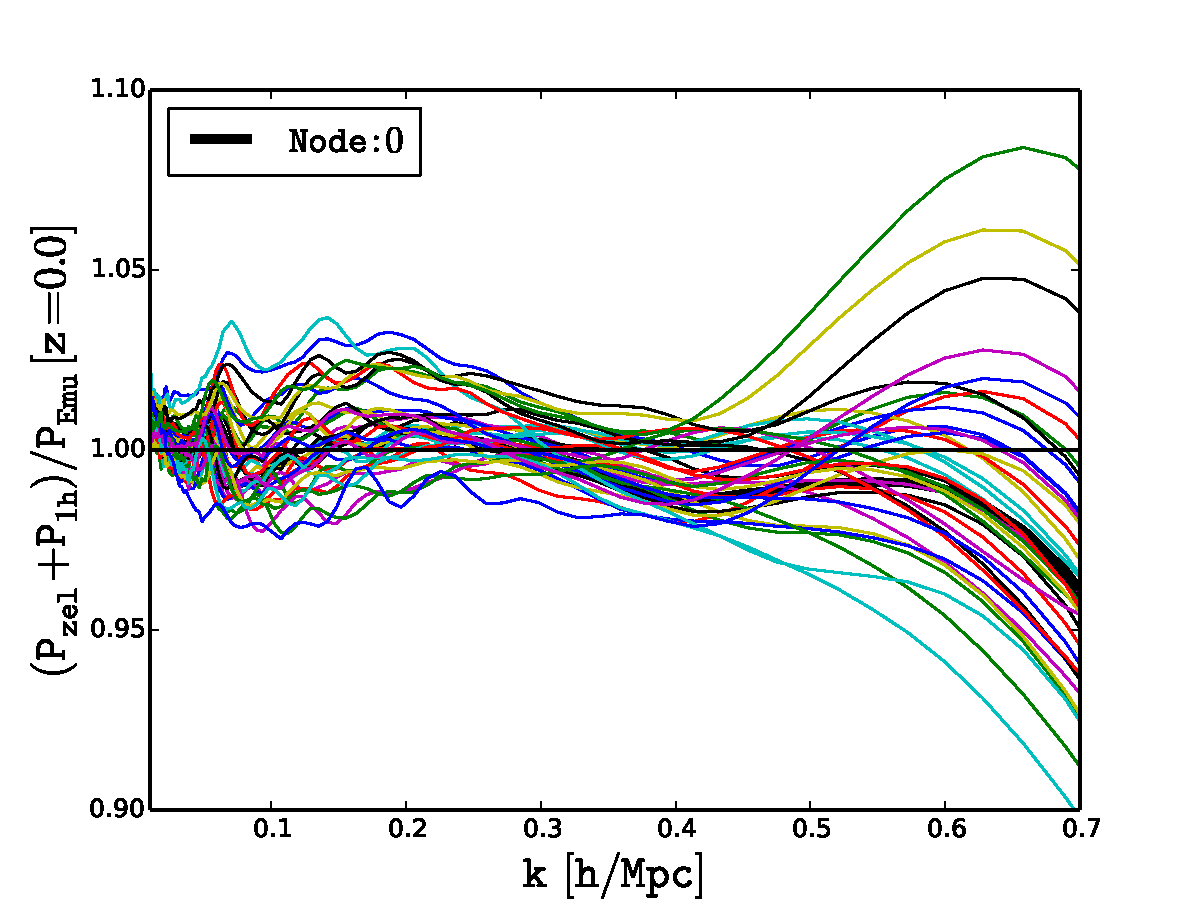
\includegraphics[width=0.48\linewidth]{figures/p2-figures/Pourmodel_Pemu_z0.0.pdf}
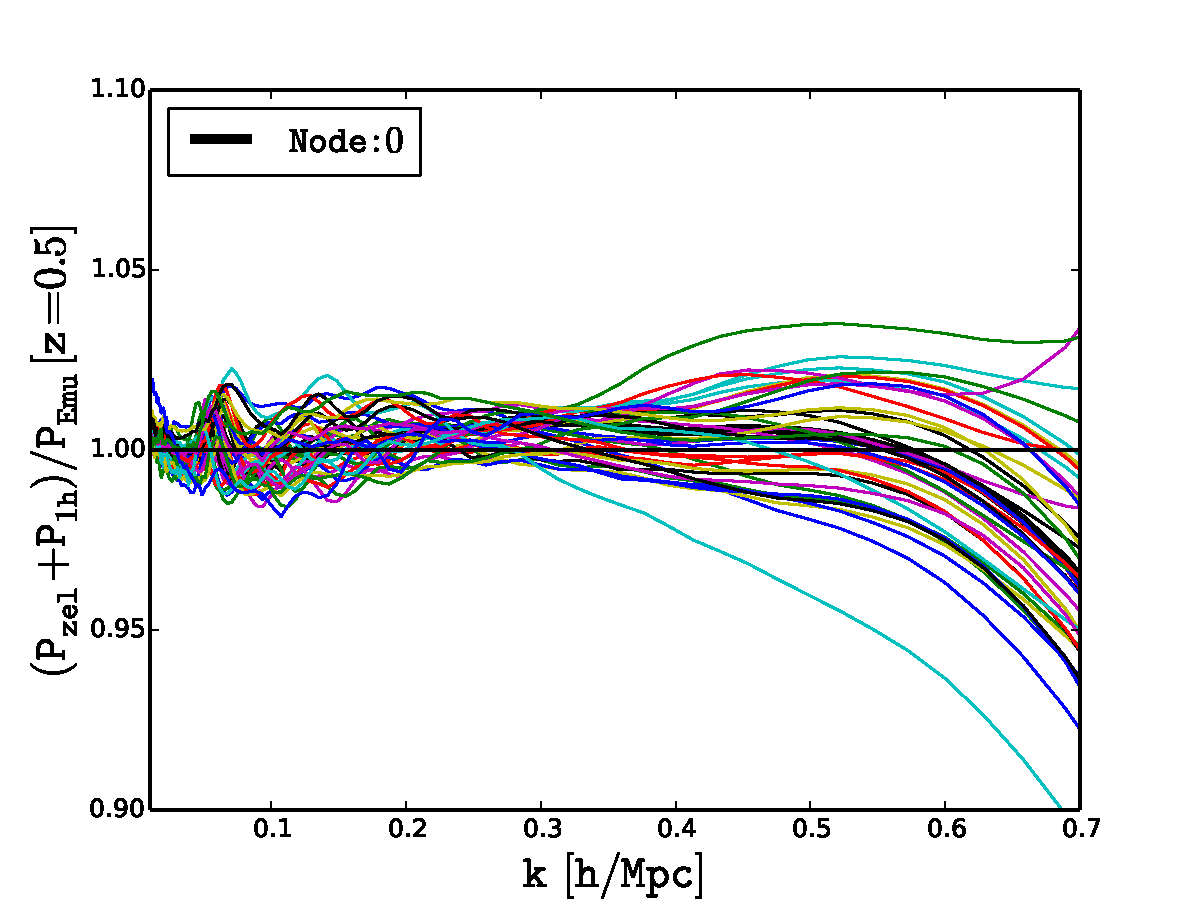
\includegraphics[width=0.48\linewidth]{figures/p2-figures/Pourmodel_Pemu_z0.5.pdf}
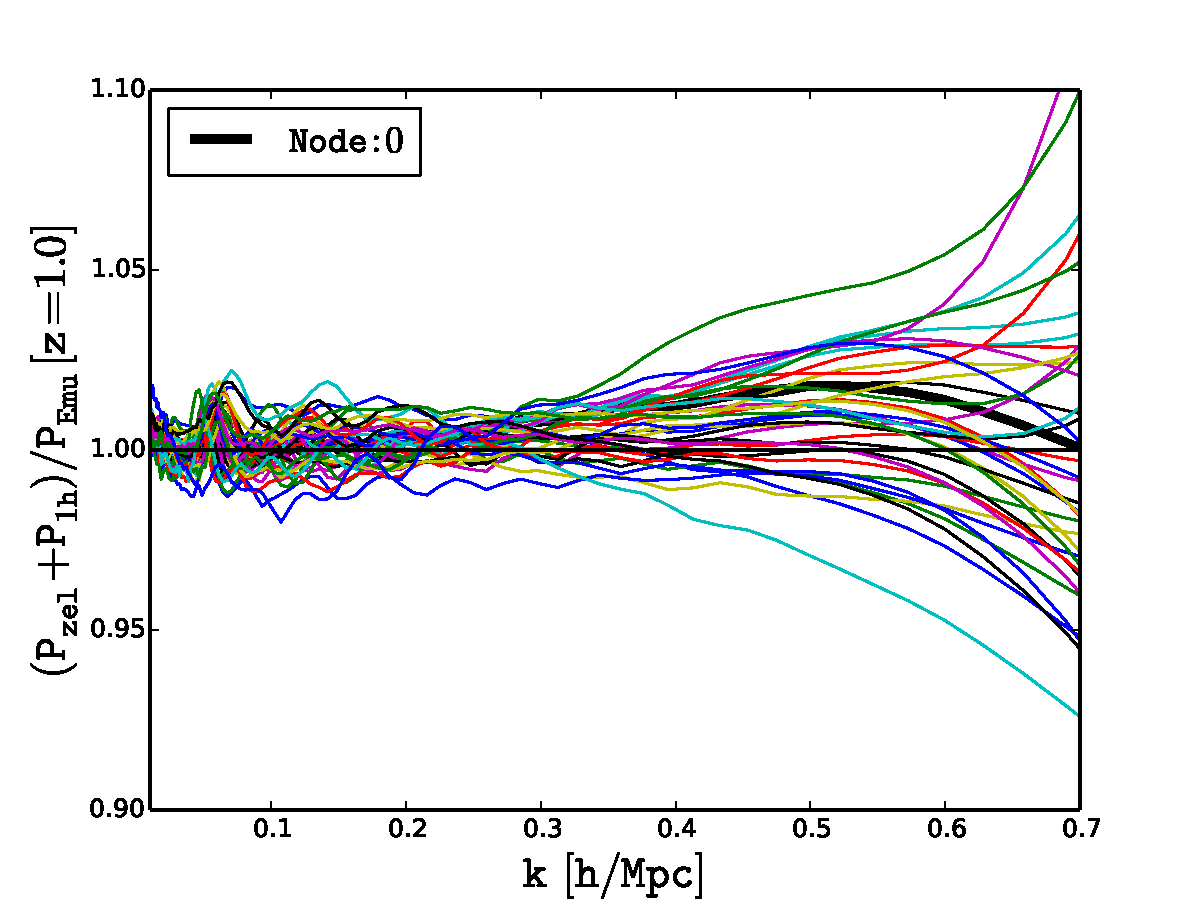
\includegraphics[width=0.48\linewidth]{figures/p2-figures/Pourmodel_Pemu_z1.0.pdf}
\caption{The residuals of our $P(k) = P_{\rm zel}(k)+P_{\rm 1h}(k)$ expression against simulations for 38 different cosmological models (different colour curves in each panel) for three different redshifts.}
\label{p2:fig:final}
\end{figure}

\clearpage



We tested this expression against the matter power spectrum from emulator ($\rm{P_{emu}}$) on 38 emulator nodes 
where the stated accuracy is 1\%. Figure \ref{p2:fig:final} shows the deviation of our predictions from the true  matter power spectrum of Emulator at three different redshifts: 0.0, 0.5 and 1.0. 
%While using $\sigma_8$ and $n_{\rm eff}$ one can predict the true non-linear matter power spectrum slightly better than using $\sigma_{11.3}$, as seen in figure \ref{p2:fig:final}, using $\sigma_{11.3}$ makes the  $A_0$ independent of $n_{\rm eff}$ and a function of $\sigma_{11.3}$ only.

At redshift 0, we can predict the power spectra to a precision of 2$\%$-3$\%$ up to $k \sim 0.5\ h \rm{Mpc}^{-1}$, 
except in some cosmologies which turn out to be unusual (typically equation of state very different 
from $w=-1$). At higher redshifts, this accuracy is even better for the same $k$, as expected since the 
nonlinear effects are smaller. For most of the cosmological models we can calculate these spectra to
5$\%$ up to $k\sim 0.7\ h \rm{Mpc}^{-1}$ and much better for lower $k$.

In figure \ref{p2:fig:node0} we show the prediction of our model for WMAP-7 cosmology (node 0)
with all its components plotted separately. Note that the $A_2k^2F(k)$ (in blue) term has a negative contribution while all other components have a positive contribution. The prediction of node 0 power spectrum is correct to about 2$\%$ up to $k \sim 0.6\ h \rm{Mpc}^{-1}$ increasing to 4$\%$ at $k \sim 0.7\ h \rm{Mpc}^{-1}$. This
can also be seen in figure \ref{p2:fig:final} where thick black line shows the ratio of the predicted and true matter power spectrum for node 0.

We also explored how well can this expression predict the changes in the matter power spectrum when 
cosmological parameters are changed. We take emulator node 0 as the fiducial model and plot the relative difference with other nodes. The first three panel of figure \ref{p2:fig:derivatives1} (in reading order) shows these derivatives for different components: linear term (in red), Zeldovich term (in green), emulator (in blue) and our predicted model (in thick black). Our predictions are matching very well with that of the true matter power spectrum from emulator, and certainly much better than pure linear theory or pure Zeldovich approximation. Note that we 
also get very good agreement of BAO smoothing, in contrast to linear theory predictions: this is because we 
are using Zeldovich approximation which smears out BAO. 
The broadband effects of Zeldovich approximation are often anti-correlated with $A_0$: this is because an 
increase in $\sigma_8$ increases the nonlinear smearing caused by the linear streaming of the 
displacement field, reducing the 
amplitude of the power spectrum in the 
Zeldovich approximation, while at the same time the amplitude of the $A_0$ is increased by the 1-halo 
term, generated by having more halos at the same halo mass. 
The latter effect typically wins: the total power spectrum and the Zeldovich power spectrum are typically, 
but not always, on the opposite side relative to the linear power spectrum. 

Of particular interest is the change in neutrino mass, also 
shown in figure \ref{p2:fig:derivatives1}. We compare the model 
predictions to the simulations of \cite{2012MNRAS.420.2551B}. We see that our model predicts nearly perfectly the changes in
the nonlinear power spectrum induced by massive neutrinos. This shows that nonlinear effects of 
massive neutrinos are no different than any other parameter: on large scales they follow linear theory, 
while on small scales the effects are dominated by the change in $A_0$. For $\sum m_{\nu}=0.15eV$ 
the change in $\sigma_8$ is about 3\% and the corresponding change in $A_0 \propto \sigma_8^{3.9}$ 
is 13\%, while Zeldovich approximation goes in the opposite direction, so the 
linear suppression of 7\% at $k \sim 0.2\ h \rm{Mpc}^{-1}$ is increased to 11\% at $k \sim 0.8\ h \rm{Mpc}^{-1}$, 
in a perfect agreement with simulations. 



\begin{figure}[p]
\centering
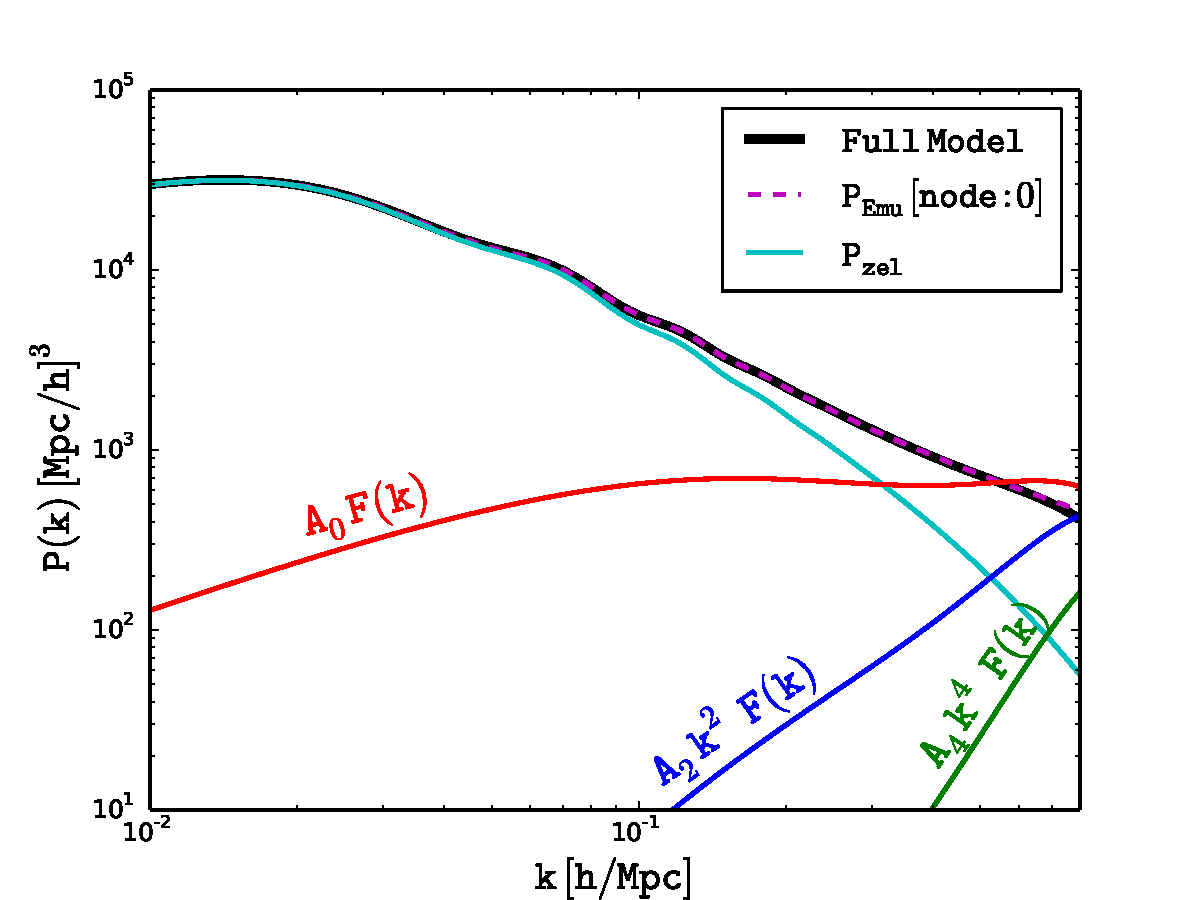
\includegraphics[width=0.95\linewidth]{figures/p2-figures/node0_pk_component.pdf}
\caption{Matter power spectrum for WMAP-7 cosmology at redshift 0.0 from simulations 
(dashed magenta line) versus Zeldovich term (cyan line), $A_0F(k)$ term (red line), $A_2 k^2 F(k)$ term (blue line), $A_4k^4F(k)$ term (green line). 
Thick Black line is the full predicted model from this work and is nearly indistinguishable from the simulations.
}
\label{p2:fig:node0}
\end{figure}

\clearpage




\begin{figure}[p]
\centering
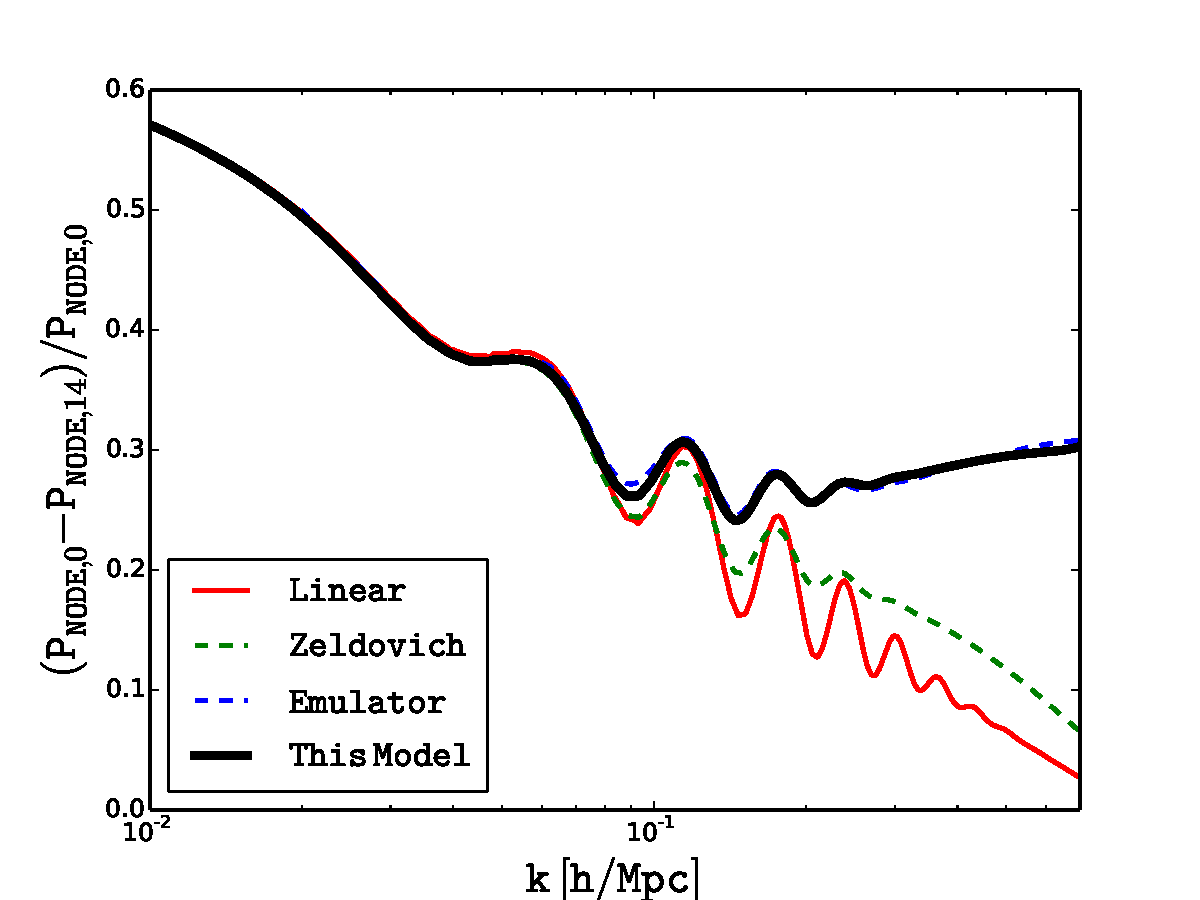
\includegraphics[width=0.48\linewidth]{figures/p2-figures/sim_linear_node14.pdf}
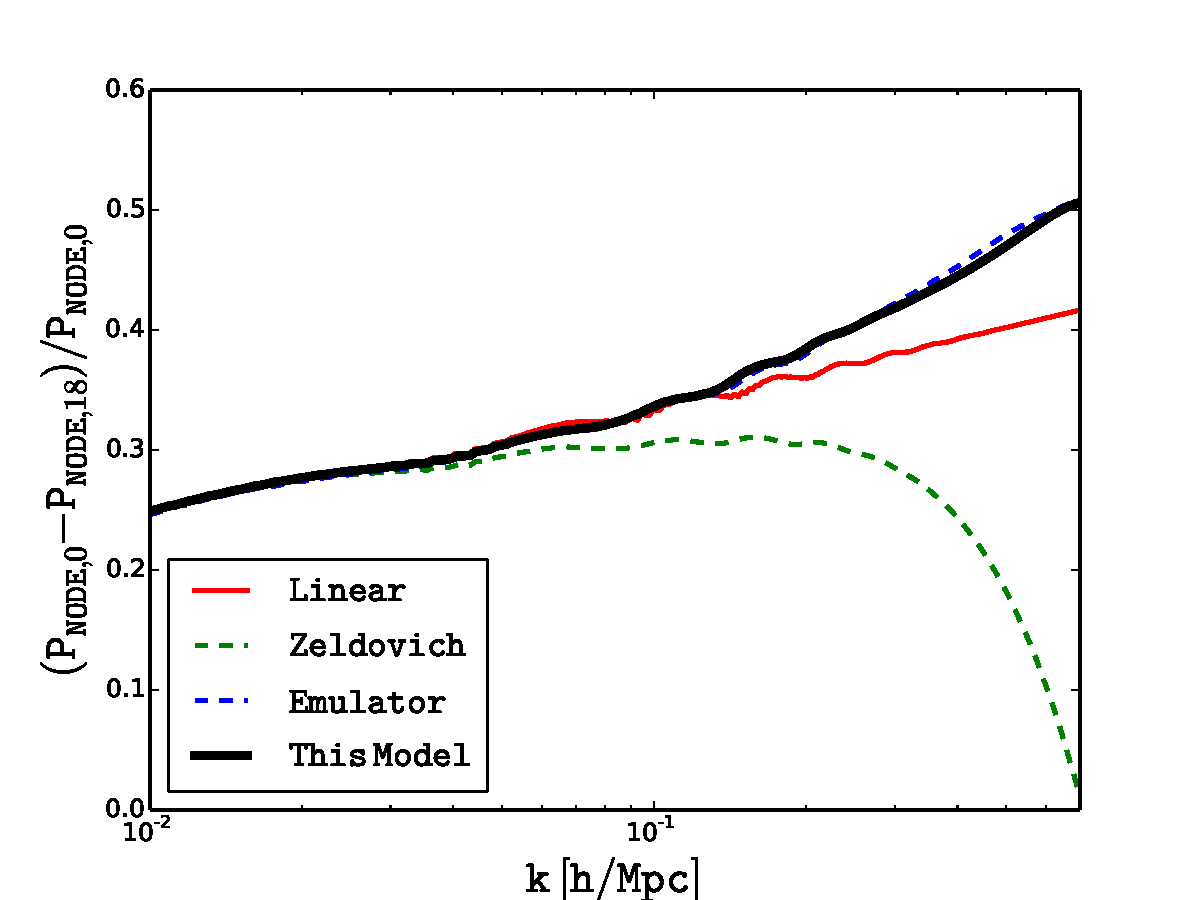
\includegraphics[width=0.48\linewidth]{figures/p2-figures/sim_linear_node18.pdf}
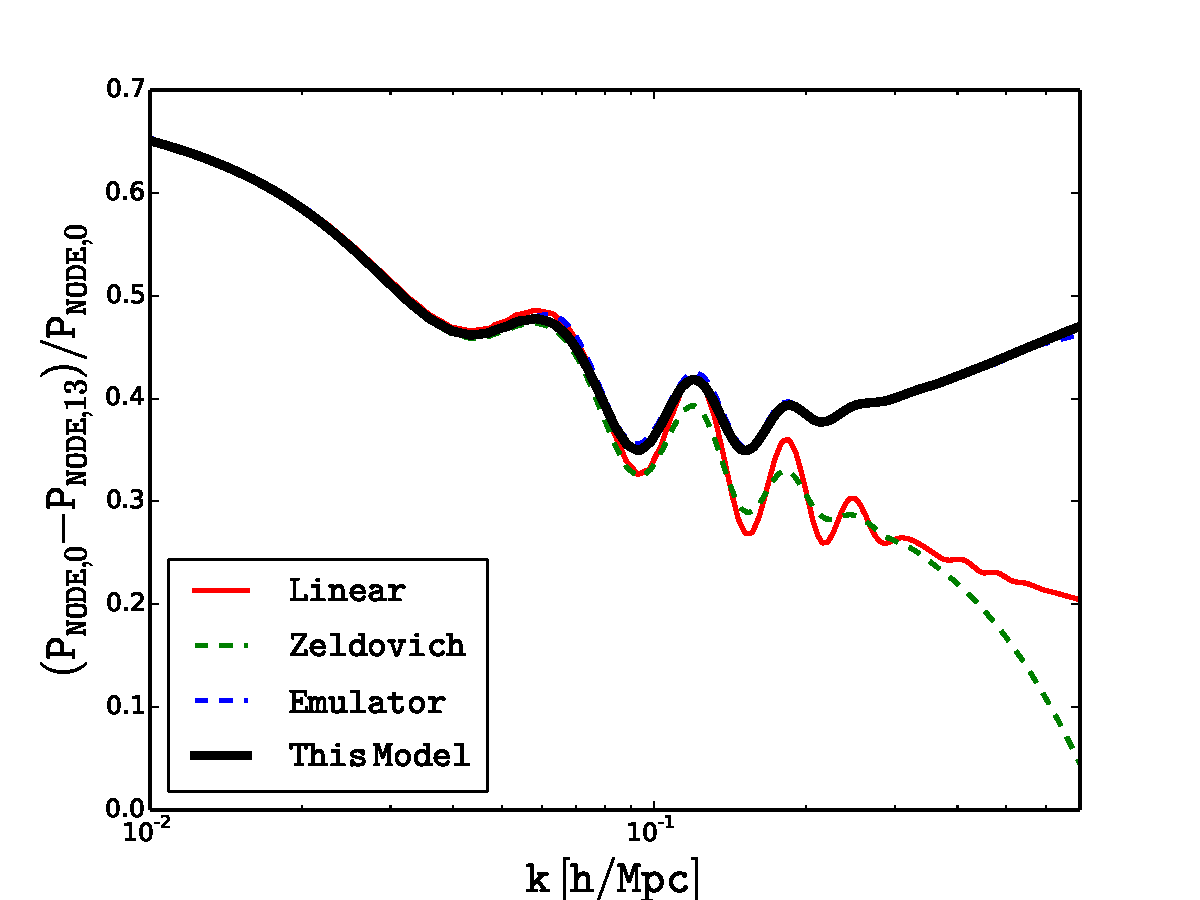
\includegraphics[width=0.48\linewidth]{figures/p2-figures/sim_linear_node13.pdf}
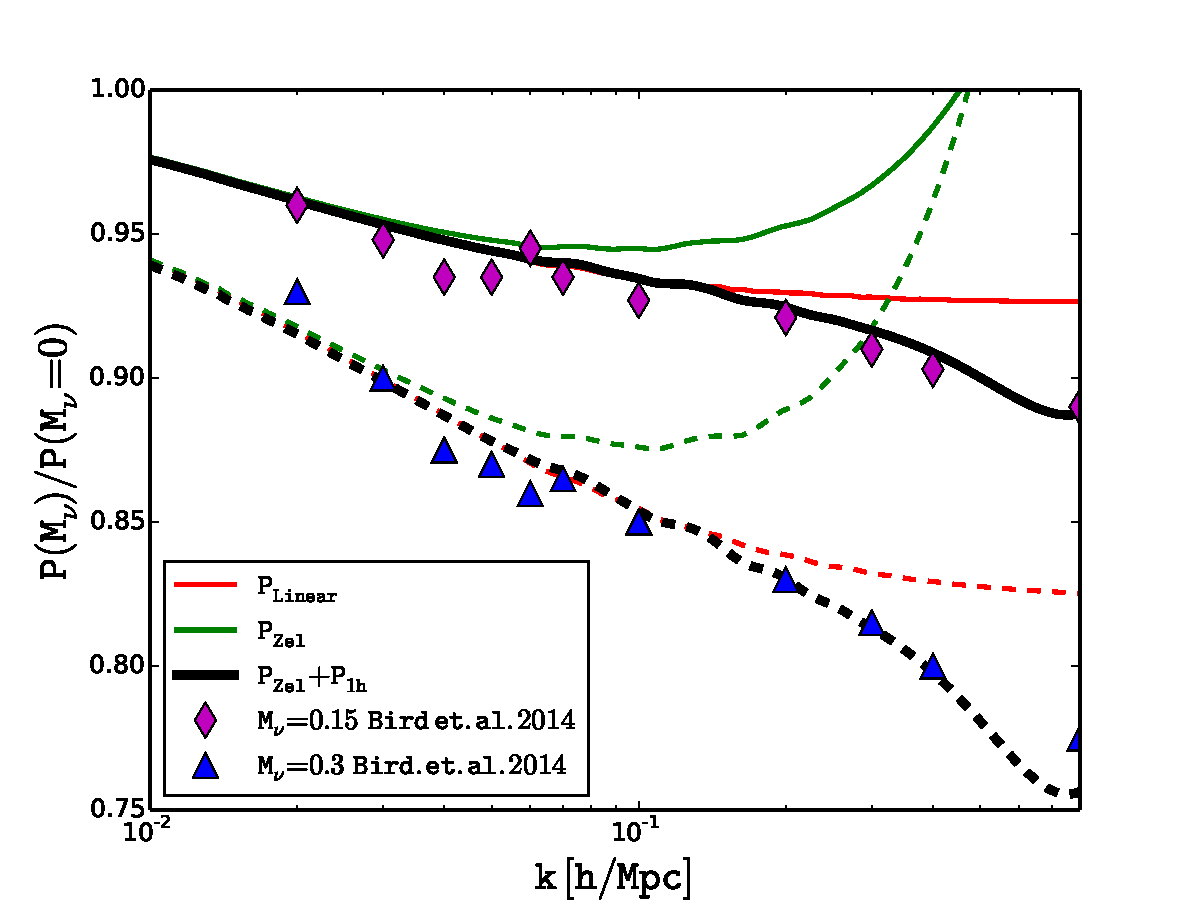
\includegraphics[width=0.48\linewidth]{figures/p2-figures/sim_linear_neutrino.pdf}
\caption{Relative difference in matter power spectrum between node 0 (Emulator) and node 14 (top-left), 18 (top-right), 13 (bottom-left). Showing the same quantity for linear term (in solid red), Zeldovich term (in dashed green), Emulator power spectrum (in dashed blue) and our prediction (in solid black). Bottom-right panel shows the ratio of the matter power spectrum with and without neutrino mass, for $\sum M_{\nu}$=0.15 (in solid lines) and 0.3 (in dashed lines) from Bird et. al. (2012).}

\label{p2:fig:derivatives1}
\end{figure}

\clearpage

%========================================================================================
\section{Covariance matrix and the cosmological information content of
  \texorpdfstring{$P(k)$}{P(k)}}
\label{p2:sec:covariancematrix}

We next turn to the issue of covariance matrix. On large scales, low $k$, the covariance matrix is based on
Gaussian approximation. 
As we move to higher $k$ the modes become correlated and the covariance matrix becomes non-Gaussian. 
In our model the non-Gaussianity comes from two separate terms. First is the non-Gaussian nature of the 
Zeldovich term and second is the non-Gaussian nature of the 1-halo term. 
We will not analyze the non-Gaussian covariance matrix in Zeldovich approximation in this paper, 
as there are currently no analytic calculations available. 
We also do not have any analytic predictions for the correlation 
between the Zeldovich part and the 1-halo part. For the 1-halo term we will focus on $A_0$ contribution, since as we will argue in next section we should marginalize over the higher order terms anyways. In our 
initial discussion we will
ignore the super-sample variance contribution \citep{2013PhRvD..87l3504T,2014PhRvD..89h3519L}, 
which will be discussed separately below. 

The halo model calculations in figure \ref{p2:fig:variance} suggest that the relative variance $\sigma_{A_0}/A_0$
should be around 0.01$\sqrt{({\rm Gpc}/h)^3/{\rm Volume}}$, depending on the cosmological model and 
redshift. 
This calculation is given by 
\begin{equation}
\left(\frac{\sigma_{A_0}}{A_0}\right)^2
=\frac{\int f(\nu)d\nu M^3}{[\int f(\nu)d\nu M]^2\bar{\rho} V},
\end{equation}
and is determined by the 4th moment of mass integrated over
the halo mass function and thus very sensitive to the halo mass function 
accuracy at the high mass end. 
Just as in the case of the halo model predictions for the scalings of $A_0$, $A_2$ and 
$A_4$, we may not completely trust the halo model predictions. 
We will write the following ansatz to the 
covariance matrix ${\rm Cov}(P(k_i),P(k_j))=\langle P(k_i)P(k_j)-\langle P(k_i) \rangle \langle P(k_j)\rangle$, 
\begin{equation}
{\rm Cov}(P(k_i),P(k_j))=P(k_i)P(k_j)
\left(\frac{2}{N_i}\delta_{ij}+\left(\frac{\sigma_{A_0}}{A_0}\right)^2\right).
\label{p2:cov}
\end{equation}
Here $N_i$ is the number of Fourier modes in the $i-$th bin. Our model predicts that the scaling of the variance is
\begin{equation}
\frac{\sigma_{A_0}}{A_0}
=\frac{\delta_{A_0}}{[(V/1 h^{-1} {\rm Gpc})^3]^{1/2}},
\,\, \delta_{A_0}=0.0079({h^{-1} {\rm Gpc})^{3/2}},
\label{p2:sigaa}
\end{equation}
where $V$ is the volume in units of $(h^{-1} {\rm Gpc})^3$, and the value of $\delta_{A_0}=0.0079({h^{-1} {\rm Gpc})^{3/2}}$
was obtained from a
fit of the model to the diagonal part of the covariance matrix derived from Planck cosmology
simulations in \cite{2014PhRvD..89h3519L}, shown in the right panel of figure \ref{p2:fig:ssv}. 
This value is slightly lower than 
the predictions of the halo model in figure \ref{p2:fig:variance}. Since the predictions are 
very sensitive to the massive end of the halo mass function, which is not well determined, we should not expect a perfect
agreement. 

It is important to note that the covariance matrix depends on the simulated volume: if the volume changes the 
covariance matrix will change, and this means that comparing one set of covariance matrix results to another is 
not trivial. We can simplify the expression if we express the number of modes in terms of a fixed width of the 
$k$ bin $\Delta k$, $N=4\pi k^2\Delta k V/(2\pi)^3$. One can see that both
the gaussian sampling variance term and the Poisson term scale with volume, so that 
\begin{equation}
{\rm Cov}(P(k_i),P(k_j))=P(k_i)P(k_j)V^{-1}
\left(\frac{4\pi^2}{k_i^2\Delta k}\delta_{ij}+\delta_{A_0}^2\right).
\label{p2:cov1}
\end{equation}
The relative contribution of diagonal versus off-diagonal terms still depends on the width of the binning in $k$, 
but the overall volume scaling is the same. 

Now that we have fixed the only free parameter of our model $\delta_{A_0}$ 
we can apply it to another set of simulations to see 
the agreement. We have compared it to results in \cite{2014arXiv1406.2713B}, which 
used 12288 boxes of size 656.25$h^{-1} \rm{Mpc}$ to derive the full covariance matrix.  
In figure \ref{p2:fig:linda} (upper panels) we have compared our model to these simulations 
for both diagonal and off-diagonal parts of the covariance matrix.
We show that 
the diagonal part of the covariance matrix (left panel of figure \ref{p2:fig:linda}) is an excellent fit, even 
better than comparison with \cite{2014PhRvD..89h3519L}, and this is without any free parameters. 
In the right panel of figure \ref{p2:fig:linda} we show the off diagonal terms for six different $k$ values. 
Our model predicts the off-diagonal correlation coefficients are simply a constant, except at the diagonal where 
there is an additional Gaussian contribution. 
Our prediction is in a reasonable agreement with these simulations: 
we are able to reproduce simulation results for both diagonal and off-diagonal terms to within 10-20\%, which is 
remarkable given its simple form and no free parameters. 
 
\subsection{Variance of the covariance matrix}

An interesting and important question is how big do the simulations need to be to converge. For the convergence of 
the power spectrum the answer is given by $\sigma_{A_0}/A_0=\delta_{A_0}/V^{1/2}$ and we can see that $V=1(h^{-1}{\rm Gpc})^3$
is sufficient for 1\% accuracy. For the covariance matrix this requirement becomes considerably stricter. One 
can write an expression for the relative variance of the covariance term as 
\begin{equation}
\left(\frac{\sigma(\sigma_{A_0})}{\sigma_{A_0}}\right)^2
=\frac{\int f(\nu)d\nu M^7}{[(\int f(\nu)d\nu M^3]^2\bar{\rho} V},
\end{equation}
so we can see that this is given by the 8th moment of the mass averaged over the halo mass function. 
The results of this prediction are shown in figure \ref{p2:fig:varvarA0}. 
The rms variance for $V=1(h^{-1}{\rm Gpc})^3$ is now about 10-30\% and the corresponding error on the 
covarince matrix (which goes as a square of $\sigma_{A_0}$) is thus 20-70\%. There is a large spread in the value because the 
calculation is so sensitive to the very high mass end of the halo mass function, which is poorly known, so the 
resulting values should only be taken as indicative and can probably vary by a factor of 2. This is simple to 
understand: occasionally there will be a large cluster formed which will significantly change the value of $A_0$, 
and consequently make its variance change considerably. 

As an example, when we compare our model predictions of the covariance matrix to \cite{2012MNRAS.423.2288H} we find that the 
agreement is not very good, in that our model predicts lower covariance matrix than measured, and the predicted value 
of $\sigma_{A_0}/A_0$ is about 40\% below the required for fit the simulations. 
However, \cite{2012MNRAS.423.2288H} used a total simulated volume of $1.6(h^{-1}{\rm Gpc})^3$, suggesting that the 
value of $\sigma_{A_0}/A_0$ has only been determined to about 10-25\%. If we let the value of $\sigma_{A_0}/A_0$
to be free, we again find a remarkable agreement with the simulations. 

To converge on the covariance matrix at 1\% one needs a simulated volume to be of order $500-5000(h^{-1}{\rm Gpc})^3$. 
This is an enormous volume: it explains why in recent work of \cite{2014arXiv1406.2713B} they needed to simulate 
12288 simulations with a total volume of $3350(h^{-1}{\rm Gpc})^3$ to converge. 

\subsection{Information content}

We can now combine the variance of $A_0$ with its scaling with $\sigma_8$, $A_0 \propto \sigma_8^{3.9}$, 
to derive the cosmology information 
content of the $A_0$ term,
\begin{equation}
\dfrac{\sigma_{\sigma_8}}{\sigma_8}=\dfrac{\sigma_{A_0}}{3.9 A_0}=0.002 \sqrt{(h^{-1}{\rm Gpc})^3/{\rm Volume}}.
\label{p2:eqn:var_s8}
\end{equation}
This is a remarkably small number, which suggests that much of the cosmological information on the 
rate of growth of structure, and consequently on the Figure of Merit for dark energy equation of state 
\citep{2010PhRvD..82f3004M}, resides in this term. To achieve a comparable precision on linear scales one would 
need about $5\times 10^5$ modes, which for $1(h^{-1}{\rm Gpc})^3$ volume 
would correspond to $k_{\rm max}=0.31\ h \rm{Mpc}^{-1}$. 
This is already well into the nonlinear regime for $z<1$ implying that we do not have this number of linear modes available, 
so the bulk of the cosmological information on the amplitude comes from $A_0$ term. 
However, since $A_0$ is mostly sensitive to amplitude (best correlation is with $\sigma_{11.3}$) 
and nothing else, this also suggests that information 
on other parameters that depend on the shape of $P(k)$ and not its amplitude will be less well 
determined. 

While we do not have reliable variance predictions for $A_2$ and $A_4$ from simulations, 
figure \ref{p2:fig:variance} suggests that $A_2$ 
has variance 3 times larger than $A_0$ and $A_4$ has variance another 3 times larger than $A_2$. 
This is mostly caused by the fact that Poisson fluctuations get larger for higher order coefficients because 
of their mass weighting: for example, $A_2$ weighting is $M^{5/3}$ as opposed to $M$ for $A_0$, giving more 
weight to higher mass halos, which are rarer and therefore have larger Poisson fluctuations. This, 
combined with less steep scaling of $A_2$ and $A_4$ with $\sigma_8$ compared to $A_0$ (equation \ref{p2:eqn:a0}, \ref{p2:eqn:a2} and \ref{p2:eqn:a4}), 
suggests that there is little additional information in these two coefficients. 
Another argument for why information in $A_2$ and $A_4$
should be ignored, based on baryonic effects, will be presented below. 


\begin{figure}[p]
\centering
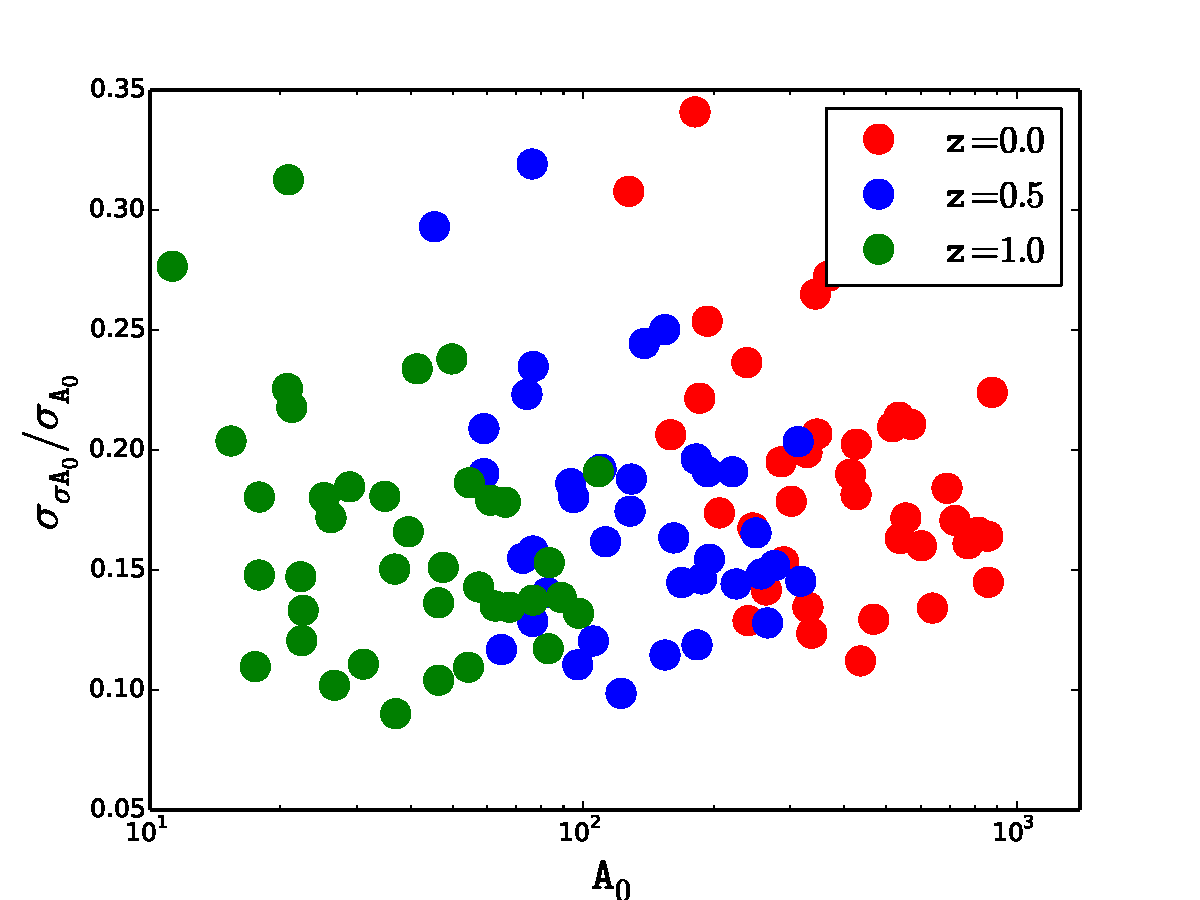
\includegraphics[width=0.8\linewidth]{figures/p2-figures/varvarA.pdf}
\caption[Relative variance of the covariance amplitude]{Relative variance $\sigma(\sigma_{A_{0}})/\sigma_{A_{0}}$ versus $A_0$ based on our model 
for three different redshifts: 0.0 (red), 0.5 (blue) and 1.0 (green). Each bullet is one cosmological realization of the 38 cosmic emulator nodes. 
 }
\label{p2:fig:varvarA0}
\end{figure}

\clearpage


\begin{figure}[p]
\centering
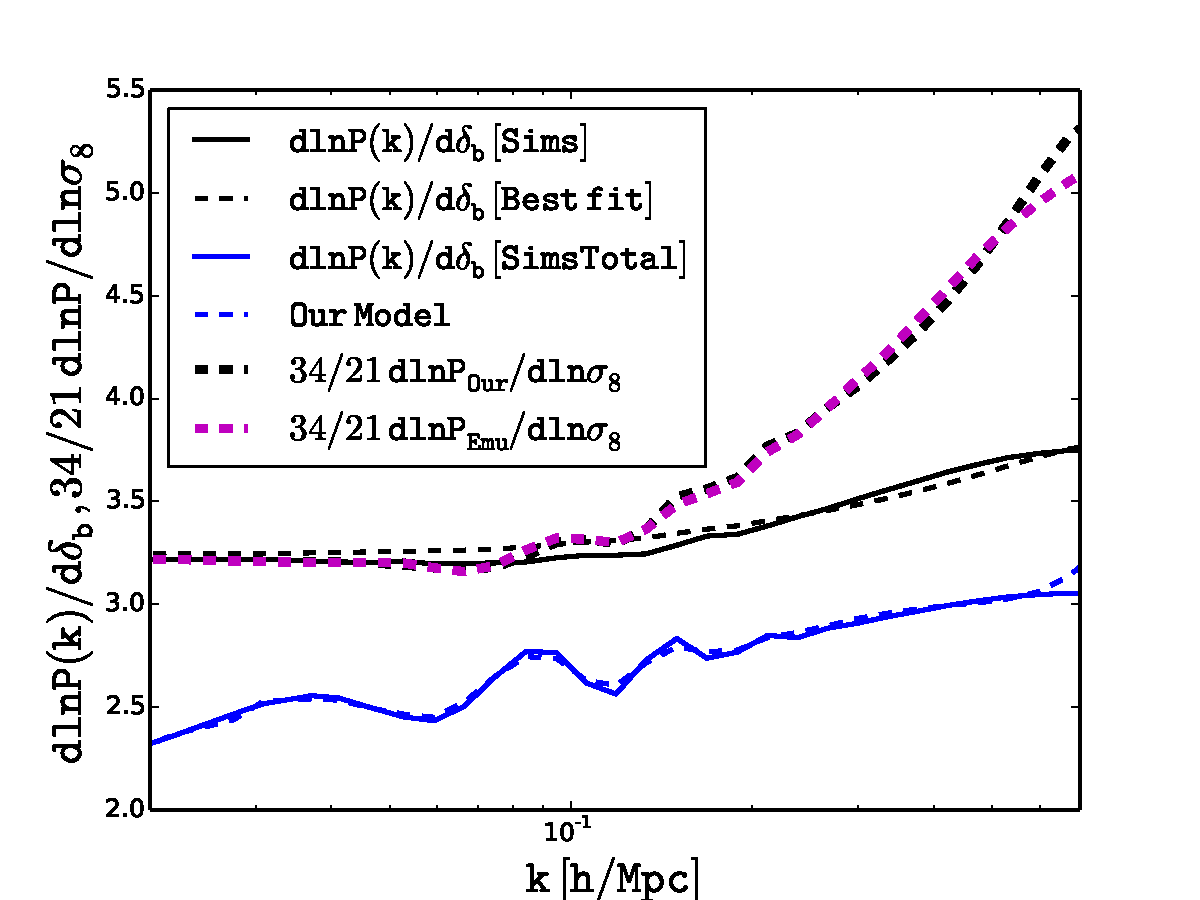
\includegraphics[width=0.48\linewidth]{figures/p2-figures/ssv.pdf}
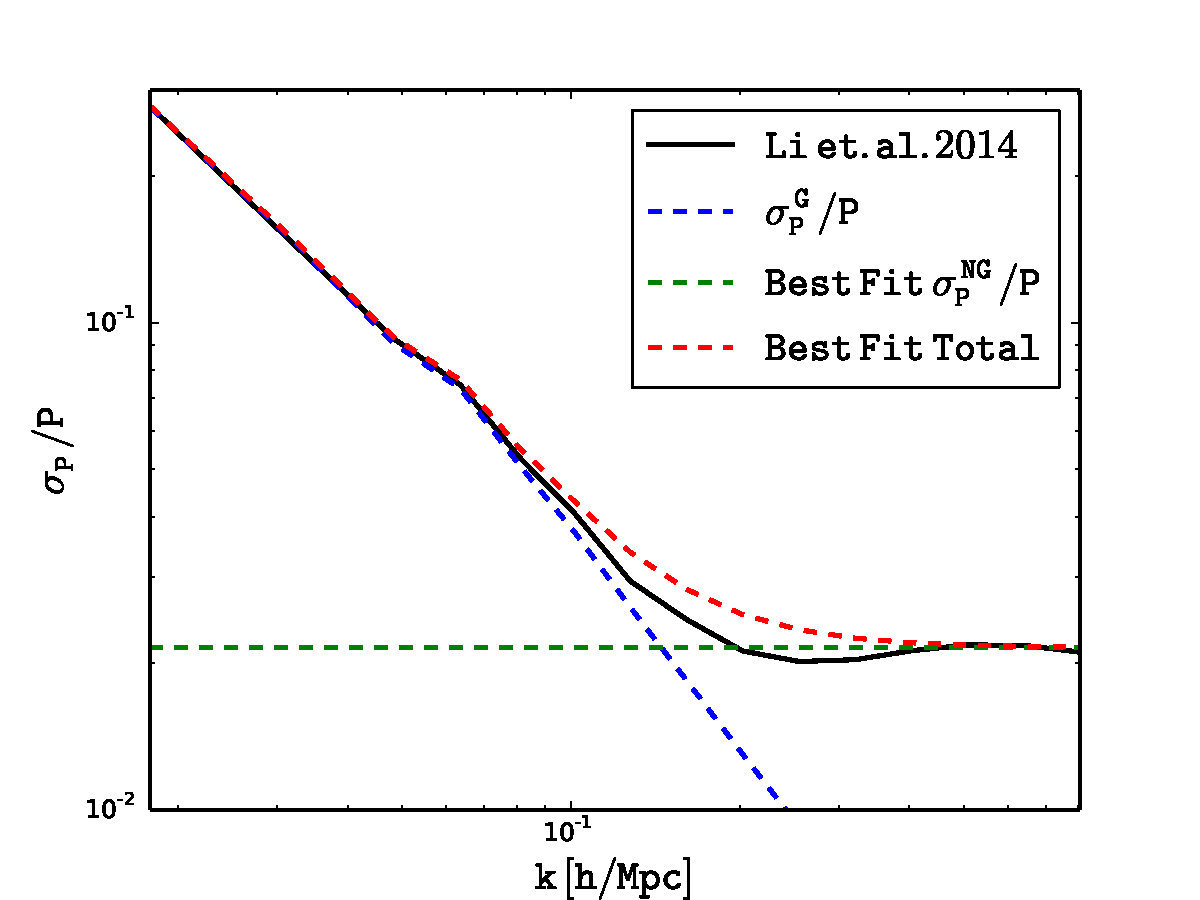
\includegraphics[width=0.48\linewidth]{figures/p2-figures/fig6.pdf}
\caption{Left: Derivative of the matter power spectrum with respect to the 
change in curvature (i.e. background density) 
from simulations (blue solid line) and our best
fit model (blue dashed line). The same, but only for the growth effect without dilation, 
is shown with the corresponding black solid and 
black dashed lines. 
The thick dashed lines show the derivative with respect to the amplitude change, such that it is degenerate 
with the curvature change at low $k$: shown are the predictions from simulations
(in magenta) and from our model (in black). We see that the degeneracy is broken at higher $k$ even in the 
absence of the dilation effect. 
Right: Relative variance in the matter power spectrum:  $\sqrt{2/N}$ (blue-dashed line) where $N$ is the number of modes, best fit $\sigma_p/P$ (green-dashed line), and the total (red-dashed line) as the norm of the two terms. }
\label{p2:fig:ssv}
\end{figure}

\clearpage


\begin{figure}[p]
\centering
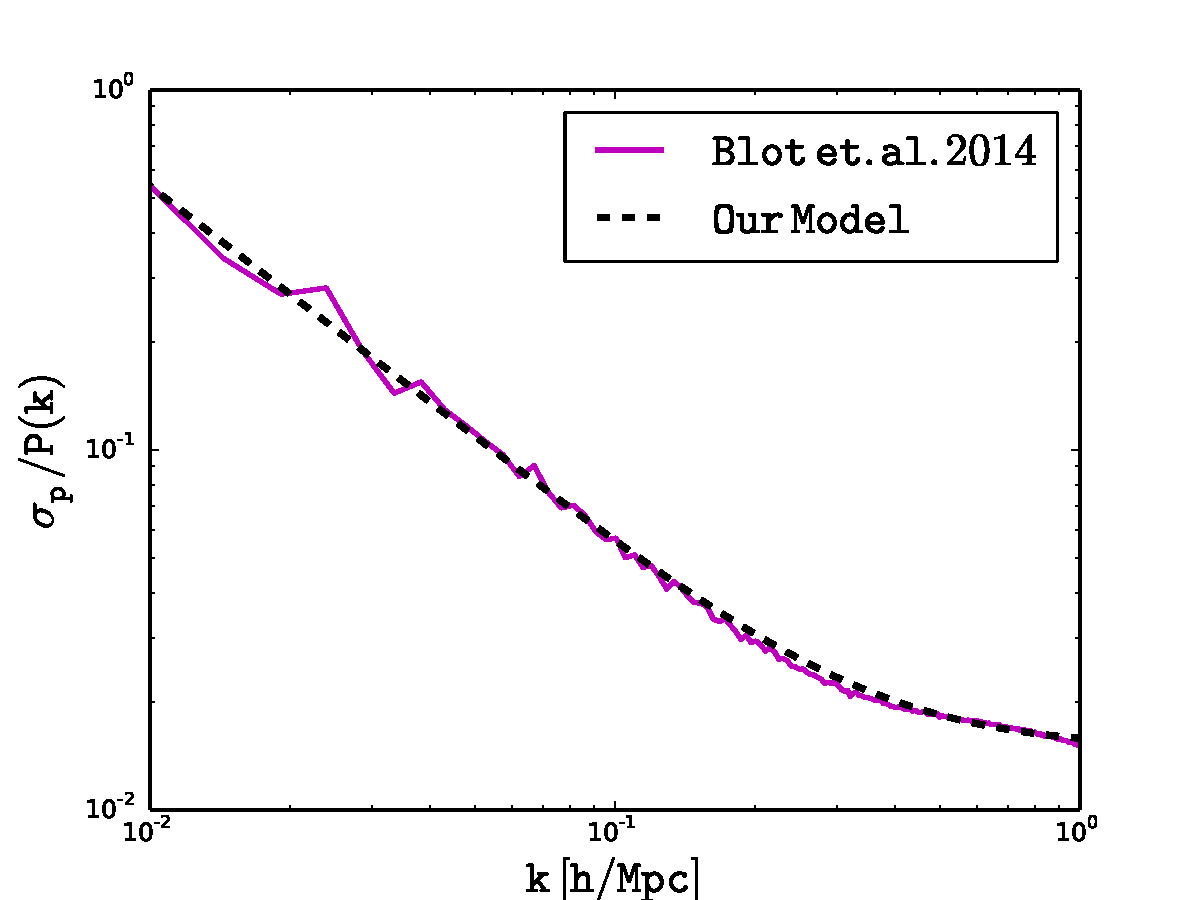
\includegraphics[width=0.48\linewidth]{figures/p2-figures/linda_diagonal.pdf}
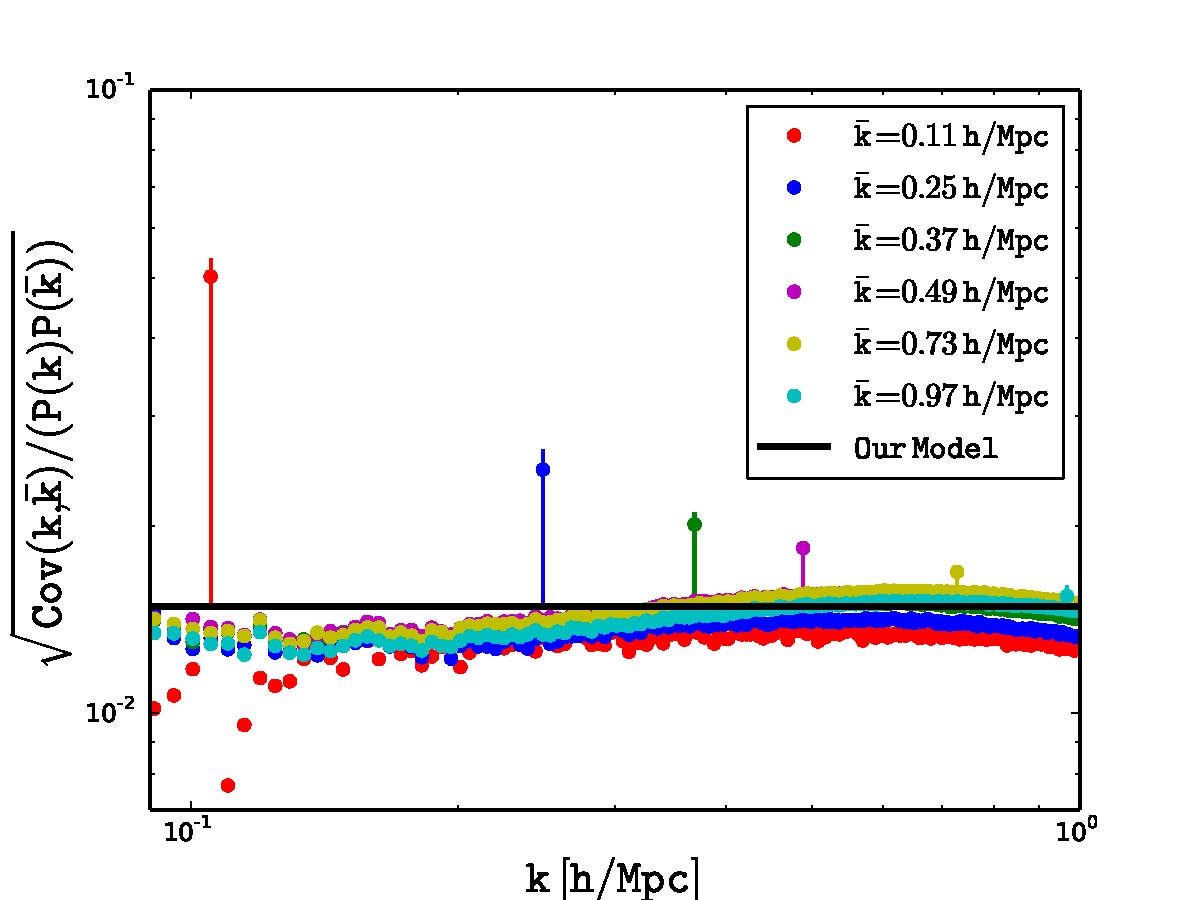
\includegraphics[width=0.48\linewidth]{figures/p2-figures/linda_offdiagonal.pdf}
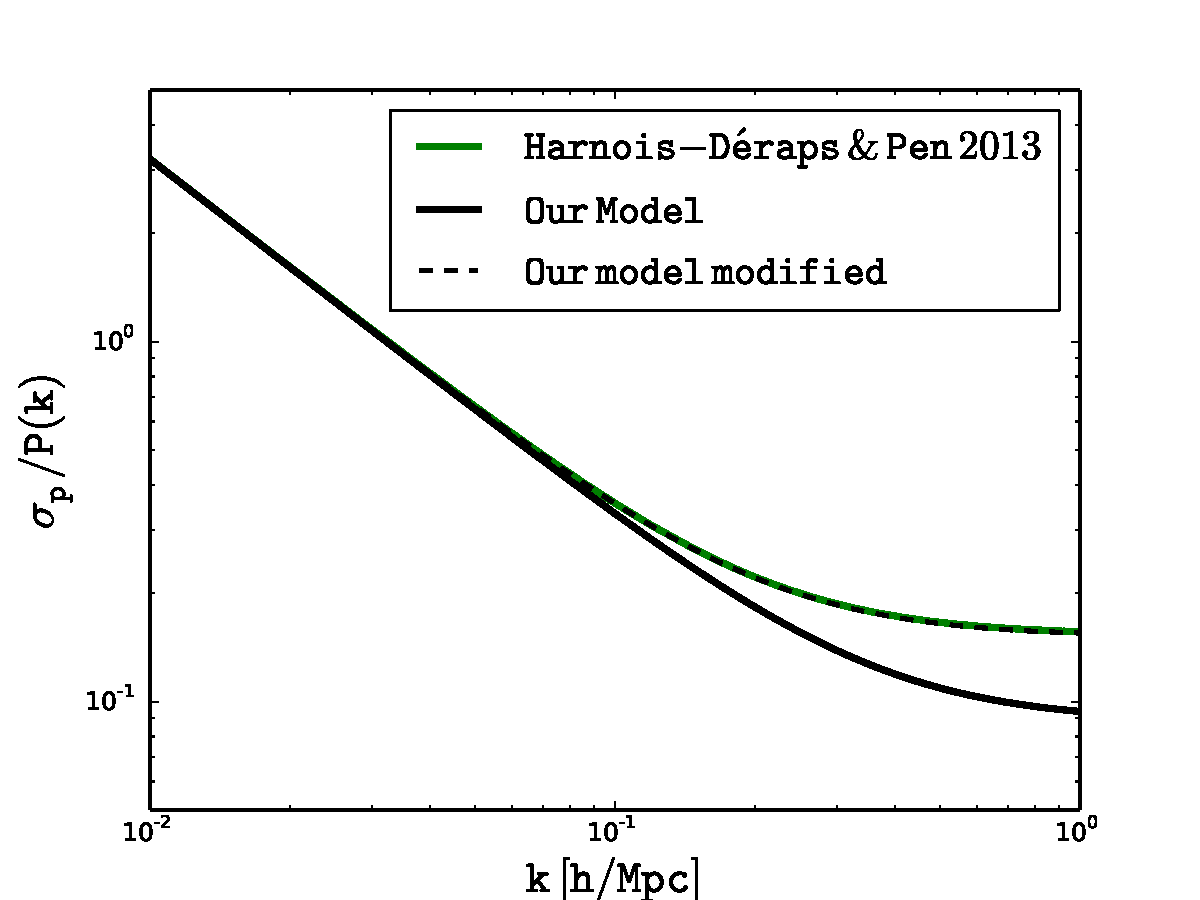
\includegraphics[width=0.48\linewidth]{figures/p2-figures/pen_diagonal.pdf}
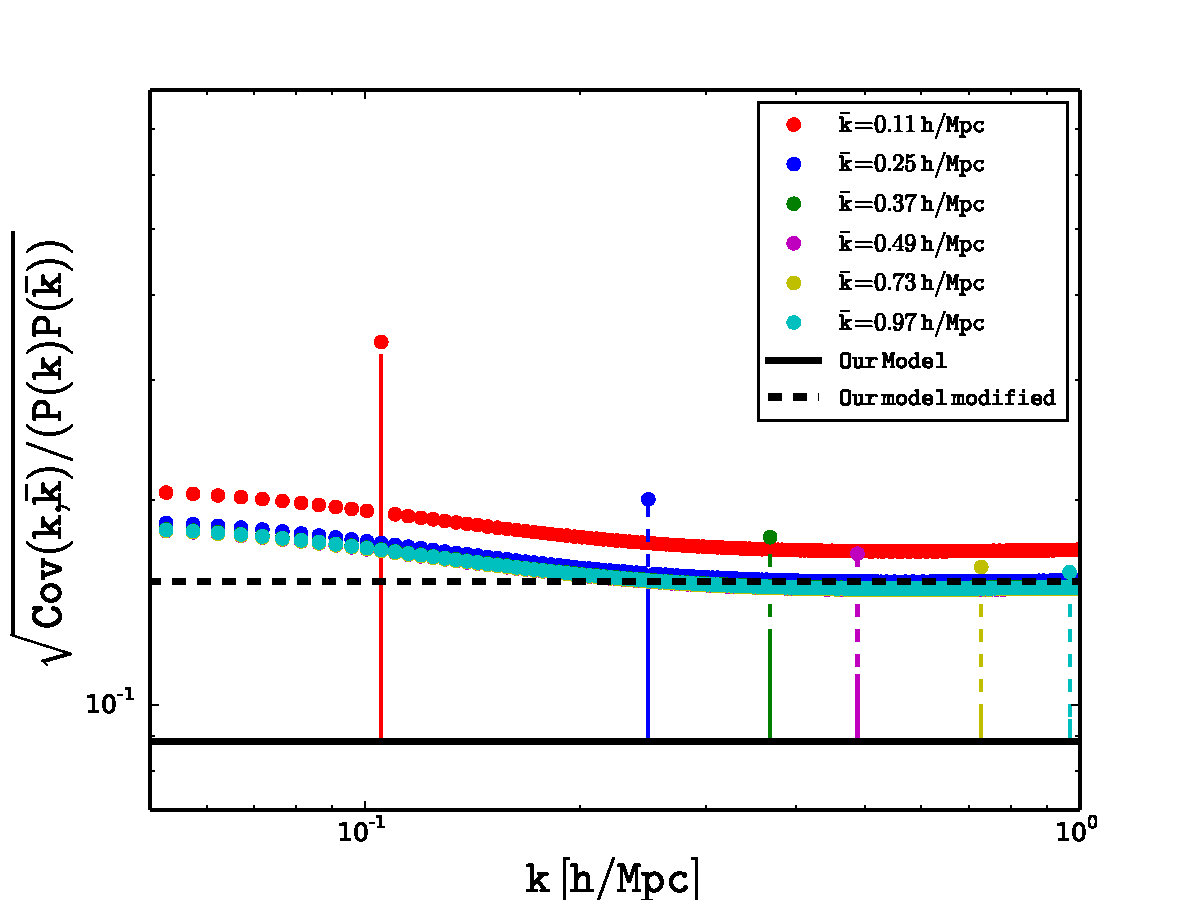
\includegraphics[width=0.48\linewidth]{figures/p2-figures/pen_offdiagonal.pdf}
\caption[Comparison of covariance-matrix predictions and simulations]{Comparison between our model prediction of covariance matrix with Blot et. al. 2014 (upper panels) and Harnois-D{\'e}raps \& Pen 2013 (lower panels) for diagonal (left panels) and off-diagonal elements (right panels). Note that there are no free parameters in the top, while for the bottom panel we show both our best model without a free parameter as well as a modified 
model where we fit for the value of $\sigma_{A_0}/A_0$, which is a valid procedure for these simulations, 
as discussed in the text. 
Our covarince matrix model (equation \ref{p2:cov}) is very simple, yet it is able to reproduce the full covariance matrix from 
simulations to within 10-20\%.} 
\label{p2:fig:linda}
\end{figure}

\clearpage


%========================================================================================
\subsection{Super-sample variance}\label{p2:sec:ssv}

Super-sample variance \citep{2006MNRAS.371.1188H} arises from the 
very long wavelength density modes that appear as constant on the scale of the survey. 
These can be viewed as a change of curvature inside the 
observed volume \citep{2011JCAP...10..031B}, and this couples to all the short wavelength modes. On large scales 
the effect can mimic a change in the amplitude of fluctuations, together with a rescaling of the 
length \citep{2012PhRvD..85j3523S}: 
\begin{equation}
\delta \ln P(k)
=\left(\frac{47}{21}-\frac{1}{3}\frac{d\ln P}{d\ln k}\right)\delta_b
=\left(\frac{68}{21}-\frac{1}{3}\frac{d\ln (k^3P)}{d\ln k}\right)\delta_b,
\label{p2:eqn:ssv}
\end{equation}
where $\delta_b$ is the density perturbation on the scale of the survey volume. 
The first term is the effect of the curvature on the growth of small scale modes, 
while the second term is the dilation due to the presence of local curvature. 
It is important to recognise that on large scales the growth 
effect is degenerate with a $(34/21) \delta_b$ change of 
amplitude $\sigma_8$, while the dilation effect of
$-\delta_b/3$ is degenerate with a change in scale, i.e. with a change in 
the angular diameter distance that can arise from a change in cosmological parameters. 
We will assume that the change in scale cannot be used as an indicator of the 
super-sample variance because of its degeneracy with these other parameters, so we will only focus on 
the change in growth rate. 
The rms fluctuations of $1({\rm Gpc}/h)^3$ volume are about 0.4\% \citep{2013PhRvD..87l3504T}, 
which together with the $34/21$ factor implies that at low $k$ one cannot determine $\sigma_8$ 
to better than 0.6\% in the linear regime, which is a factor of 3 larger error than the error on $\sigma_8$ 
without the super-sample variance in equation \ref{p2:eqn:var_s8}. It is therefore clear that without addressing this issue the 
super-sample variance dominates the errors. 

On smaller scales we expect the nonlinear effects  are no longer degenerate with a change in $\sigma_8$. 
Physically the reason for difference is in the curvature nature of the super-sample
variance: curvature effects grow with the growth rate, i.e. the growth of short wavelength mode $\delta_s$ due to the 
coupling to the long wavelength mode
scales as $\delta_s(z)[1+34D(z)\delta_{b0}/21]$, where $D(z)$ is the linear growth rate and $\delta_{b0}$ is the long 
wavelength mode today,  and thus this coupling only matters
at low redshifts since $D(z)\ll 1$ for $z\gg 1$. This
is different from a simple change in overall amplitude $\delta_s(z)(1+\delta \sigma_8)$, which has no redshift dependence. 

To understand this more quantitatively we can compute the logarithmic 
derivative of $A_0$ (equation \ref{p2:A024}) with respect to the 
two parameters in the context of the universal halo mass function $f(\nu)$, where $\nu$ is given by equation \ref{p2:nu}
\citep{2008JCAP...08..031S}. 
The Lagrangian bias is defined as $b_L=\bar{n}^{-1}\partial n/\partial \delta_b$, which can be rewritten using 
$\nu=(\delta_c-\delta_b)^2/\sigma^2$ as $b_L=(-2\nu/\delta_c)\partial \ln[\nu f(\nu)]/\partial \nu$. 
In addition we also have the mean density increased by $\delta_b$ inside the patch. We are still dividing
the density with the 
global mean density, so $\bar{\rho}$ does not change. 
Using this we find 
\begin{equation}
\frac{d \ln A_0}{d \delta_b}
=\frac{\int (1+b_L(\nu)) \nu f(\nu) M d\ln \nu}
{\int \nu f(\nu) M d\ln \nu}
=\langle (1+b_L) \rangle. 
\end{equation}
So the logarithmic slope of $A_0$ with respect to a long wavelength modulation is given by the appropriate 
average of the Eulerian bias $b_E=1+b_L$. 

If instead one looks at the logarithmic growth of the amplitude with respect to amplitude $\sigma_8 \propto \sigma(M)$, 
then $d\nu/d\ln \sigma_8=-2\nu$, and so 
\begin{equation}
\frac{d \ln A_0}{d \ln \sigma_8}
=\delta_c\frac{\int b_L(\nu) \nu f(\nu)M d\ln \nu}
{\int \nu f(\nu)M d\ln \nu}
=\delta_c \langle b_L \rangle.
\end{equation}
Since $d \ln A_0 /d\ln \sigma_8 = 3.9$ we find $d \ln A_0 / d \delta_b = 3.9/1.68+1 = 3.3$. 
The response to the long wavelength mode has thus a lower logarithmic slope of growth relative to $\sigma_8$ and 
is not much larger than the linear regime value $68/21$. This should be contrasted against the response to the 
amplitude change, which goes from $\sigma_8^2$ in the linear regime to $\sigma_8^{3.9}$ in the nonlinear regime. 
Note that this calculation is valid if the density is divided by the global background density, as appropriate 
for weak lensing observations, which are sensitive to the total density. Whenever the density perturbation is 
defined using local mean density these numbers should be reduced by 2. 

Numerical results are shown in the left panel of figure \ref{p2:fig:ssv}, where we show the nonlinear response to $\delta_b$ from 
simulations of \cite{2014PhRvD..89h3519L}, and the corresponding response to a change in $\sigma_8$ that mimics 
$\delta_b$ at low $k$. 
We can still model a change in $\delta_b$
as a quasi-linear term and $(A_0-A_2k^2+A_4k^4)F(k)$. For the quasi-linear term we adopt 
%Zeldovich approximation with the corresponding change in $\sigma_8$, or 
simply the Zeldovich approximation 
model multiplied with the corresponding linear factor of $68/21\delta_b$, and we fit for 
the other three parameters. The result is shown in figure \ref{p2:fig:ssv} and 
provides a reasonable fit to the simulations. Note that we show results with and without 
$d\ln P / d\ln k$ term, against simulations with and without it \citep{2014PhRvD..89h3519L}. 
We find that for 
$\delta_b=0.02$ $A_0$ has changed by 7.4\%, while the quasi-linear term has changed by 6.4\%, so that 
$d\ln P/d\ln \delta_b=3.2$ at low $k$ and $3.7$ around $k \sim 0.5\ h \rm{Mpc}^{-1}$ where $A_0$ dominates. This is 
in a reasonable agreement with the analytic estimate of 3.3. 
For the $\sigma_8$ scaling a change of 6.4\% in the linear term corresponds to 
13\% change in $A_0$. 
The contrast between the two effects is shown in figure \ref{p2:fig:ssv}. The super-sample variance 
is thus not degenerate with $\sigma_8$, so if one can determine both the quasi-linear term and 
$A_0$ term with sufficient accuracy, one can break the degeneracy between the two effects. 


How well can one determine $\sigma_8$ in the presence of super-sample variance? 
If we only have information from $A_0$ then the analysis above suggests that one can determine 
$\sigma_8$ to about $(3.7/3.9)0.4\% \sim 0.38\%$ in $1(h^{-1}{\rm Gpc})^3$ volume, about a factor of 2 worse than 
without the super-sample variance. If we have information both from linear regime and from $A_0$ 
dominated regime then we can break the degeneracy between the super-sample variance and $\sigma_8$. 
The extent to which this can be achieved depends on how well we can measure the amplitude in the 
linear regime: to reach 0.4\% accuracy we would need to measure all the modes up to $k \sim 0.2\ h \rm{Mpc}^{-1}$
in a $1(h^{-1}{\rm Gpc})^3$ volume, which seems possible to achieve. Moreover, we note that a change in 
curvature cannot be modeled well with just a change in linear term and $A_0$, higher order terms also 
change significantly. Even though we argue below that these effects are degenerate with baryonic effects, 
this degeneracy may be broken in this situation given how different these effects are and given that 
there is a lot of information present at high $k$. 
In summary, the amplitude of fluctuations in 
a $1(h^{-1}{\rm Gpc})^3$ volume can be determined to an accuracy of 0.4\% if the super-sample 
variance cannot be determined, which can be reduced by a factor of 2 if the degeneracy between the super-sample 
variance and $\sigma_8$ amplitude can be broken. 

Instead of including the super-sample variance 
effect in the covariance matrix one can include it as an additional curvature parameter that 
one can marginalize over. The parameter is $\delta_b$ and its prior should be a Gaussian with a
zero mean and rms variance $\sigma_V$ determined by the survey window (see \cite{2013PhRvD..87l3504T,2014MNRAS.441.2456T} for predictions for 
simple survey geometries). The response of the power spectrum to the long wavelength 
$\delta_b$ parameter should be 
\begin{equation}
\delta P=\left(\frac{47}{21}P_{\rm Zel}-\frac{1}{3}\frac{dP}{d\ln k}
+\left[3.7A_0-3A_2k^2+2.5A_4k^4 \right]F(k)\right)\delta_b,
\end{equation}
where $P_{\rm Zel}$, $A_0$, $A_2$ and $A_4$
are the values of the fiducial model around which we are exploring the super-sample variance effect. 
For  example, in a MCMC chain this would be 
the model one is testing at a given chain position. 
We found that the fit to the simulations must include $A_2$ and $A_4$ terms and that the fit is only 
valid to $k \sim 0.7\ h \rm{Mpc}^{-1}$. Note that the change of $A_2$ and $A_4$ relative to $A_0$ is 
similar to that of amplitude change in equation \ref{p2:slopea024}.   


%========================================================================================
\section{Effects of baryons}
\label{p2:sec:baryons}

\begin{figure}[p]
\centering
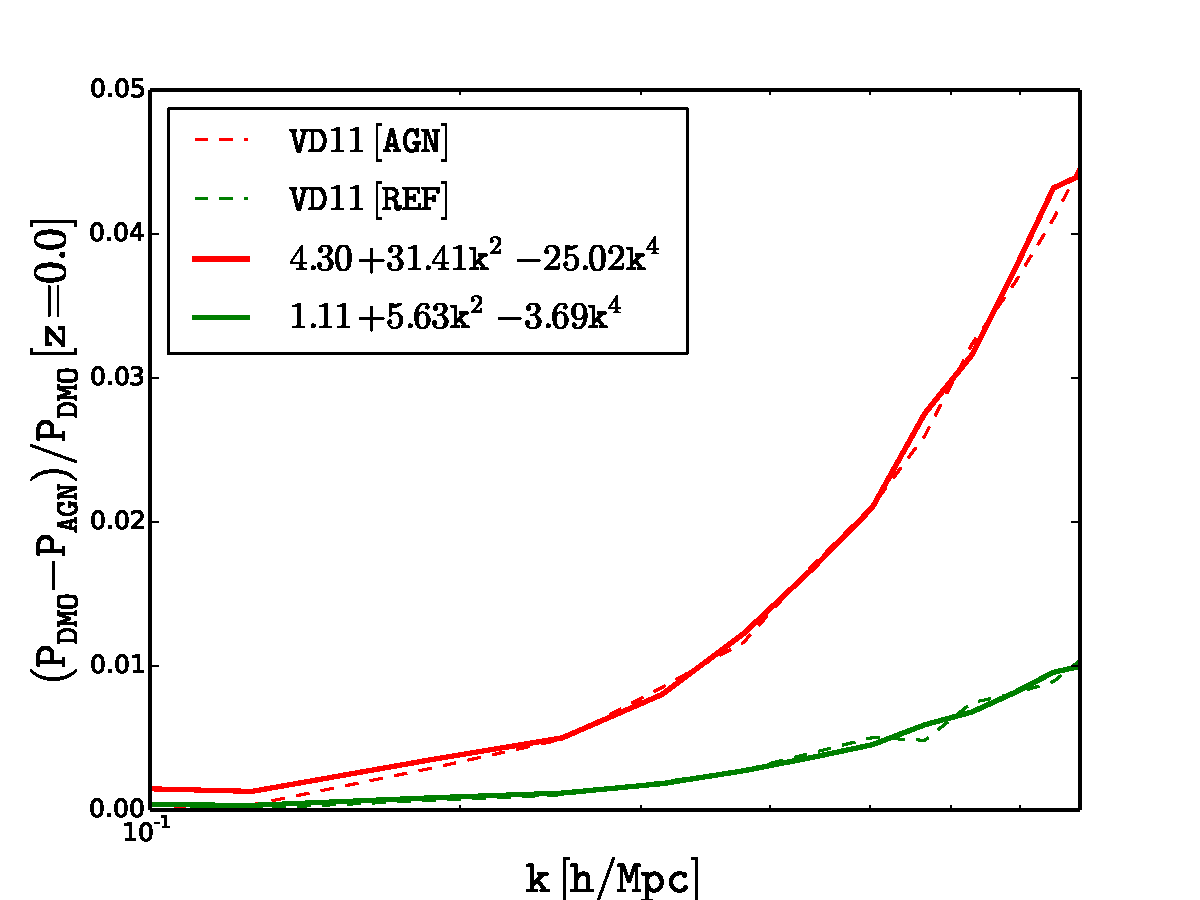
\includegraphics[width=0.48\linewidth]{figures/p2-figures/fit_dmo_agn_z0.0.pdf}
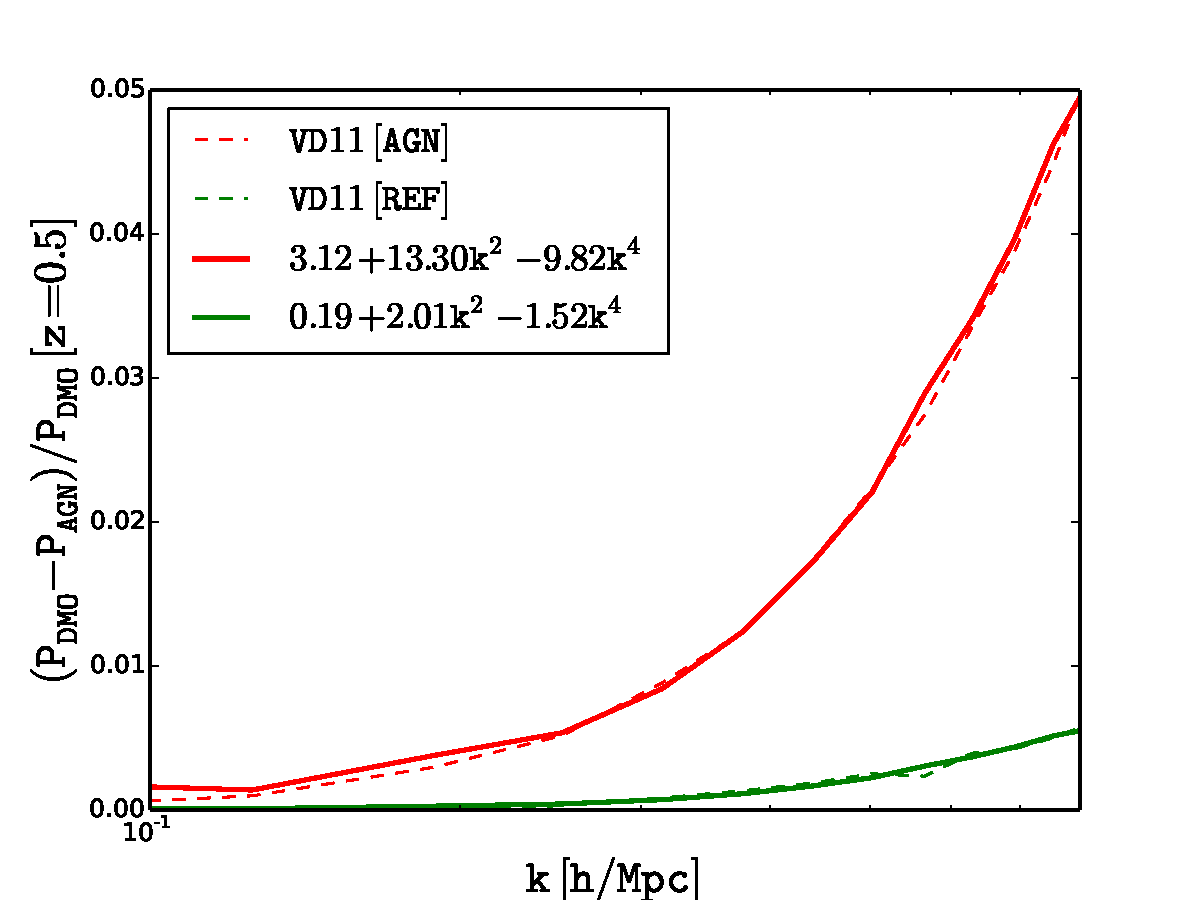
\includegraphics[width=0.48\linewidth]{figures/p2-figures/fit_dmo_agn_z0.5.pdf}
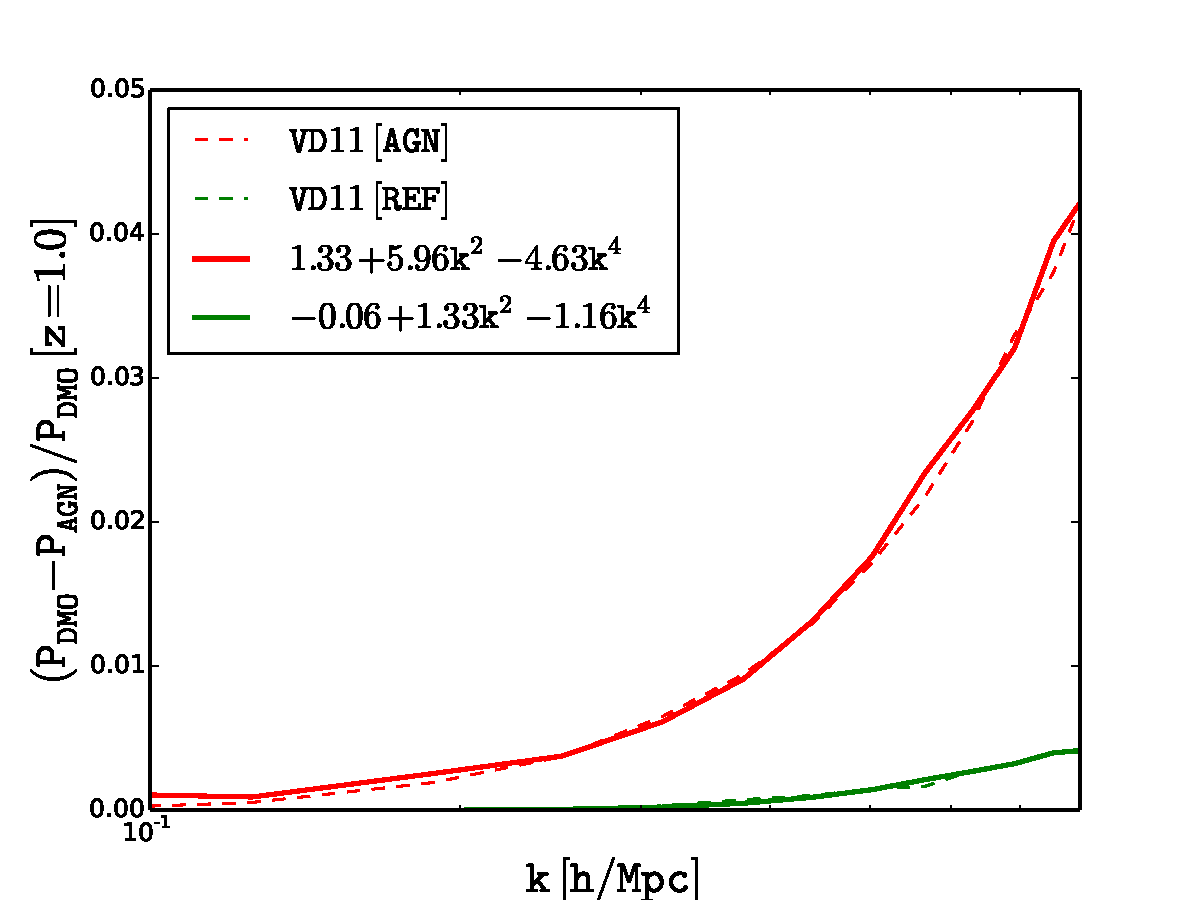
\includegraphics[width=0.48\linewidth]{figures/p2-figures/fit_dmo_agn_z1.0.pdf}
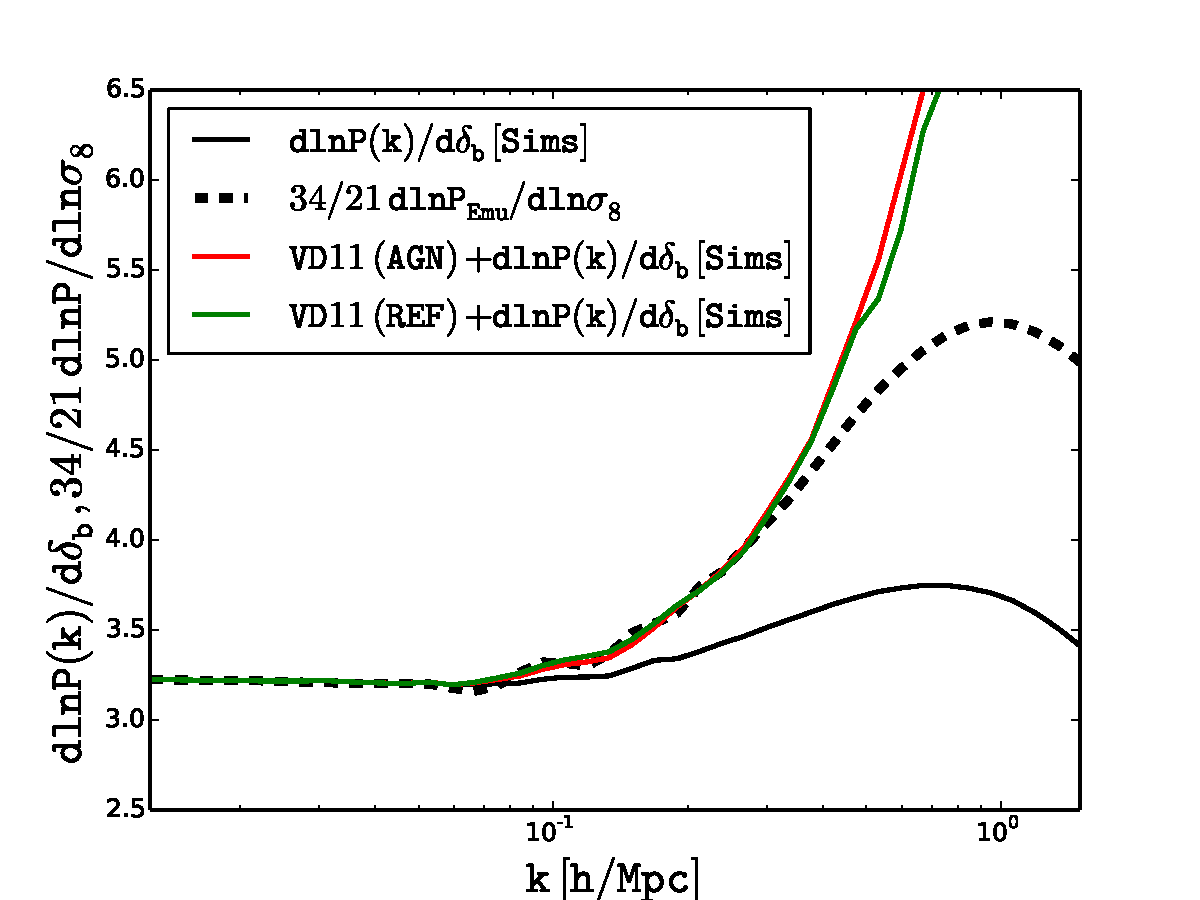
\includegraphics[width=0.48\linewidth]{figures/p2-figures/baryons.pdf}

\caption{The first three panel (in reading order) are the relative difference between DM only model and AGN (red-dashed line) and REF (green-dashed line) from van Daalen et. al. 2011 (VD11) at redshift 0.0 (top-left), 0.5 (top-right) and 1.0 (bottom-left). REF model contains the baryonic physics without any AGN feedback model. Solid lines (red and green) are the corresponding best fit $\delta A_0-\delta A_2k^2 + \delta A_4k^4$ as explained in section \ref{p2:sec:baryons}. Bottom-right panel shows the derivative of the matter power spectrum with respect to a change in background density (2$\%$) in solid-black from Li et. al. 2014, and with respect to a change in 
amplitude using prediction from emulator (thick dashed-black line).} 
\label{p2:fig:baryons}
\end{figure}

\clearpage


Baryonic effects inside the dark matter halos change the matter power spectrum relative to the dark matter 
alone and these effects must be incorporated into the analysis, otherwise they can lead to substantial bias 
in the cosmological parameter estimation \citep{2011MNRAS.417.2020S,2013MNRAS.434..148S}. 
Baryonic effects can come in different forms. First is 
simply the fact that gas distribution inside dark matter halos is distributed differently than the dark matter, 
because gas is hot and has significant pressure. As a result, gas has a core at the center of the cluster, leading 
to reduced clustering strength on small scales. Second effect is baryon cooling, which causes gas to cool and 
condense into galaxies at the dark matter halo centers. This leads to an enhancement of the clustering relative 
to pure dark matter case. Baryons can also be pushed out of the halo centers by processes such as 
supernova and AGN feedback, which can in some cases push the gas quite far out. Furthermore, in all of these
examples dark matter may also be redistributed as a consequence of the baryons either condensing onto the 
halo centers or being pushed out. For example, 
for baryonic cooling onto a galactic disk this process is known as adiabatic contraction \citep{1984Natur.311..517B}.  

From the halo model point of view the main effect of the baryons is the redistribution of the gas, and possibly 
dark matter, inside the halos. This can be qualitatively described as the change in the 
scale radius $R_s$. The total mass of the halo $M$ is unchanged, since these baryonic processes do not push the 
gas or the dark matter far out of the virial radius of the halo such that the halo mass would be affected. 
As a consequence, we expect that $A_0$ parameter is essentially unchanged, while $A_2$, $A_4$ etc. will change 
during the baryonic redistribution of matter. 

To investigate this further we used simulation based matter power spectra from \cite{2011MNRAS.415.3649V} to compute
the effects of baryons on the coefficients $A_0, A_2$ and $A_4$. In particular, we use the dark matter only 
 and the supernova and AGN feedback models, corresponding to hydrodynamical simulations with supernova or
AGN feedback model. It was argued that the latter is needed to reproduce 
cluster observations such as X-ray luminosity temperature 
relation \citep{2010MNRAS.406..822M}. We use the AGN model as the main model 
since it provides the largest effects, but we also explore reference supernova feedback model from 
\cite{2011MNRAS.415.3649V}. 
Baryon corrections to the matter power spectrum from AGN feedback model 
exceed one percent level for $k> 0.3 \ h \rm{Mpc}^{-1}$ \citep{2011MNRAS.415.3649V}. 
We use the results at three different redshifts: 0.0, 0.5 and 1.0. In figure \ref{p2:fig:baryons} we try to fit the difference between the pure dark matter and AGN model, $\rm{P_{DMO} - P_{AGN}}$, or reference supernova feedback
model $\rm{P_{DMO} - P_{REF}}$, with the model
$\delta A_0 + \delta A_2k^2 + \delta A_4 k^4$, 
to estimate the changes in these coefficients due to baryons at
each redshift (note that since the changes are only important at high $k$ we can set 
$F(k)=1$). We fit these models over the $k$ range between 0.2 and 0.8 $\ h \rm{Mpc}^{-1}$. Figure \ref{p2:fig:baryons} 
shows the best fit models, which are a good fit to the simulations over this range. 
We also calculated these coefficients for the cosmology assumed in this paper using the results from figure \ref{p2:fig:A_sigma}.

We find that for the AGN model the relative change in $A_0$ is about $0.5-1\%$, depending on the redshift, 
whereas the changes in $A_2$ and $A_4$ are about $4-7\%$ and 4-8 $\%$, respectively. 
If we assume no change in $A_0$ the fit is a bit worse and
the change in $A_2$ and $A_4$ is larger. 
This confirms that the coefficient $A_0$ is quite indifferent to baryonic effects, while
$A_2$ and $A_4$ are significantly more contaminated. 
The change is positive. This is expected since AGN feedback expands 
the gas and makes the scale radius $R_s$ larger. It is less obvious why $A_0$ should increase when gas is being pushed 
outwards, but the effect on $A_0$ is small and it could also be driven by the numerical fitting procedure. 
If we assume that the baryonic uncertainty is at the level suggested by these AGN models, then using 
equation \ref{p2:eqn:covariance} the 
corresponding uncertainty on $\sigma_8$ will be $0.5-1\%/3.9 \sim 0.1-0.2\%$ from $A_0$, and about an 
order of magnitude larger from $A_2$ and $A_4$. Given that the difference between AGN and DM models is probably 
an overestimate of the error associated with the baryonic effects our analysis
suggests that these effects can be effectively 
marginalized over without any loss of cosmological information from $A_0$. 
We also note that other baryonic feedback models from \cite{2011MNRAS.415.3649V}, such as the 
reference model, while giving a lower amplitude of 
the effect, have very similar $k$-dependence, as can be seen from figure \ref{p2:fig:baryons}. 



Above we argued that super-sample variance effect should not be treated as a variance but as a separate 
parameter that can be determined from the data. Using linear theory and $A_0$ may not contain enough information 
to break the degeneracy between the amplitude $\sigma_8$ and super-sample variance. Using higher $k$ information may be 
more promising, since the two effects also have very distinctive signatures on $A_2$, $A_4$ etc. Since our 
model expansion to $A_4$ only works to $k \sim 0.7\ h \rm{Mpc}^{-1}$ we explore this question numerically. 
In figure \ref{p2:fig:baryons} bottom-right we plot the 
super-sample effect and amplitude effect such that they are degenerate at low $k$, while also adding the
baryonic effect 
such that it is degenerate with change of amplitude up to $k \sim 0.3\ h \rm{Mpc}^{-1}$. 
We see from the figure \ref{p2:fig:baryons} that above $k \sim 0.3\ h \rm{Mpc}^{-1}$ 
the degeneracy is broken: the effects of $\sigma_8$ and $\delta_b$ are smaller compared to 
the effect of AGN 
feedback, which
continuous to increase with $k$, because gas is being pushed out on small scales, suppressing all small 
scale clustering. While this analysis is only restricted to a specific form of baryonic effects and is less robust 
than the other analyses in this paper, it suggests that one may be able to break the degeneracy between the 
baryonic effects, cosmological parameters such as amplitude, and super-sample variance, using high $k$ information. 


%========================================================================================
\section{Discussion and conclusions}\label{p2:sec:discussion}

In this work we propose a model of the matter power spectrum using the Zeldovich approximation
power spectrum as the 2-halo term and even powers of $k$ expansion of the 1-halo term, compensated 
on large scales to satisfy mass conservation, with coefficients 
calibrated on simulations. The leading order 1-halo term is $k^0$ term amplitude $A_0$, which
in the halo model can be determined as a mass dependent integral over the halo mass function.
Simulations predict $A_0 \propto \sigma_8^{3.9}$, and the halo model is only able to reproduce this at low 
redshifts. 
The amplitude of $A_0$ is related to the cluster 
abundance method, where one counts clusters above a given mass, which also depends on the halo mass
function and has a similarly 
steep dependence on $\sigma_8$. It is also related to SZ power spectrum 
scaling, which is dominated by the 1-halo term and scales
as $\sigma_8^7$ \citep{2002MNRAS.336.1256K}, because the SZ signal from individual clusters 
scales as $M^{5/3}$ rather than 
halo mass $M$ and it is a projection over line of sight, leading to a steeper dependence on $\sigma_8$.
Our analysis thus explicitly connects the cluster abundance method to the amplitude of the leading nonlinear 
correction to the matter power spectrum, and shows the two use similar information. As a consequence, these two 
methods cannot be combined independently if the dominant errors are Poisson or large scale structure fluctuations. 

Using the first 3 coefficients of expansion 
we accurately predict variations of basic cosmological parameters up to $k\sim 0.7\ h \rm{Mpc}^{-1}$, including amplitude 
$\sigma_8$, matter density $\Omega_m$, Hubble parameter $H_0$, primordial slope $n_s$, 
equation of state $w_0$ and even neutrino mass $\sum m_{\nu}$. In all cases our model predicts well the BAO 
smoothing, a consequence of using the 
Zeldovich approximation rather than linear theory for the 2-halo term. 

We present a very simple 
model for the covariance matrix of matter power spectrum (equation \ref{p2:cov}). 
We stress that the covariance matrix depends on the simulated volume both in linear and 
nonlinear regimes, so a direct comparison between covariance matrices from 
different simulations needs to account for this. 
In this model the large scale variance is dominated by the 
sampling variance, while 
on small scales where $A_0$ dominates the dominant term is the Poisson sampling of the halos. 
Using the halo mass function  of \cite{2008ApJ...688..709T} to predict the latter gives about 20-30\% higher value than 
fitting with simulations of \cite{2014PhRvD..89h3519L}, which we consider a good agreement given the 
inaccurate nature of halo mass function fits in the high mass regime.
Using this value we 
show that our model gives a remarkable agreement with 
the simulations of \cite{2014arXiv1406.2713B}, where 12288 simulations of $656 h^{-1}{\rm Mpc}$ box size were run to 
construct a covariance matrix. 
We use our Poisson model to compute the convergence rate of the covariance matrix and find that simulated 
volumes of 500-5000$(h^{-1}{\rm Gpc})^3$ are needed to converge at 1\% level. This explains why our model without any free parameters 
does not reproduce covariance matrix 
\cite{2012MNRAS.423.2288H}, because the total volume used in \cite{2012MNRAS.423.2288H} 
was only 1.6$(h^{-1}{\rm Gpc})^3$, and has thus not converged with high enough accuracy. 
Changing the parameter $\sigma_{A_0}/A_0$ from 
the predicted 0.09 to 0.15 we obtain a perfect agreement. 

Using this model we argue that most of the cosmological information about the amplitude 
is in $A_0$, which can determine the amplitude $\sigma_8$ to 0.2\% within $1(h^{-1}{\rm Gpc})^3$ volume. 
The higher order coefficients $A_2$, $A_4$ etc. 
are less sensitive to $\sigma_8$ and have a larger variance.
We discuss the super-sample variance and argue that due to its origin as a curvature effect it
differs from the amplitude rescaling and so it 
should be treated as a separate cosmological parameter with a 
prior given by the rms variance on the scale of the survey volume. 
If its degeneracy with the amplitude is not broken then it approximately doubles the errors, so that 
$\sigma_8$ can be determined to 0.4\% within $1(h^{-1}{\rm Gpc})^3$  volume. Note that both of these errors are a lot 
smaller than the currently available constraints, which at best are at 
4\% \citep{2013MNRAS.430.2200K}: observational and modeling errors 
dominate the error budget 
at the moment, but future data sets may be able to reach the levels where super-sampling variance 
or Poisson error will dominate \citep{2012PhRvD..86h3504Y}. 

We also investigate the baryonic effects on the matter power spectrum. We argue that these 
should not change $A_0$ much because of the mass conservation. Indeed, comparison of our model to 
simulations of baryonic effects in \cite{2011MNRAS.415.3649V} suggests that $A_0$ is almost unchanged, while higher order 
coefficients change significantly, because baryonic effects redistribute gas and dark matter 
inside the halos without changing the overall halo mass. 
We advocate that marginalizing over higher order expansion coefficients 
should immunize against baryonic effects without much loss of information. We explore the degeneracy 
between the amplitude, super-sample variance and baryonic effects, finding that it can be broken using 
information above $k \sim 0.3\ h \rm{Mpc}^{-1}$. 

Our results suggest that analytic modeling of dark matter clustering provides important insights 
even in the era of large simulations. 
It offers a promising 
venue not only for an accurate power spectrum description, but also for the covariance matrix modeling, 
for optimal extraction of information from the data, and for description of baryonic effects. 
We have shown that in the context of covariance matrix calculations our model is likely to be more reliable 
than simulations with insufficient total volume. 
However, more work remains to be done before it can be applied to the weak lensing observations. 
For example, 
in this paper we focused on the dark matter clustering description in terms of its
power spectrum. If one wants to apply the method
to the weak lensing observations one needs to perform the line of sight projections of the model onto the weak
lensing power spectrum $C^{\kappa \kappa}_{l}$, where $\kappa$ is the convergence which can be 
written as a projection of the density along the line of sight. Projecting powers of $k$ simply gives the same 
powers of $l$, so if the projection kernels are narrow, as would be the case for weak lensing 
tomography, the analysis remains essentially 
unchanged, except for the fact that weak lensing probes matter density rather than density 
perturbations, so convergence is also multiplied by an overall mean 
matter density. If the projection kernels are broad and there are significant 
contributions from nearby structures for which $k>0.7\ h \rm{Mpc}^{-1}$ projects to a low $l$, then one
needs to assess these effects and improve the model to account better for the high $k$ contributions. 
Similarly one also needs to project baryonic effects and covariance matrix. 
This program is feasible and if implemented it will give a completely analytical 
description of the weak lensing power spectrum and its covariance matrix
without any need to use simulations. 

\section{Acknowledgements}
We thank Z. Vlah for extensive discussions and for providing the Zeldovich power spectrum code, F. Schmidt and M. Takada for
useful comments, Y. Li for electronic form of the plots of \cite{2014PhRvD..89h3519L}, M. van Daalen for electronic form of the plots of \cite{2011MNRAS.415.3649V}, L. Blot for providing us data from their simulations, and J. Harnois-Deraps and U. Pen for interpretation of their covariance matrix.
U.S. is supported in part by the NASA ATP grant NNX12AG71G. I.M. would like to thank the hospitality of LBNL.



%==============================================================================
% Chapter 4: Paper 3
%==============================================================================

\chapter{Baryonic Effects on Weak-Lensing Two-Point Statistics}
\label{p3:chap:baryonic-effects}

\section{Introduction to the Paper}

According to the Dark Energy Task Force (DETF; \cite{2006astro.ph..9591A}), 
the two-point statistics of the weak gravitational lensing is amongst the most promising
tools to do cosmology and derive strong constraints on the cosmological parameters. 
However, it is dominated by many systematics, both observational and theoretical.
In this paper, we focussed on an extremely important source of systematic errors in the 
theory of weak lensing shear power spectrum - {\it baryonic effects}. 

The theoretical modelling of the weak-lensing shear power spectrum
is described in section \ref{sec:wl} for a dark-matter only Universe, 
which is a fair approximation
at large scales, which was the limit to the weak-lensing experiments in the past. 
The next generation surveys like Euclid, LSST etc., 
are pushing this limit far into the small scales such
that baryonic contribution becomes important. In this paper, we built a model
to incorporate baryonic contribution in the matter power spectrum,
and by extension to the weak lensing shear power spectrum. Our model is based on 
the halo model where the baryonic contribution is sensitive to mainly two quantities: 
the halo mass function, and the radial density profiles of the halos.

Our baryonic model consists of four main ingredients: 
(i) hot intra cluster gas assumed to be in hydrostatic equilibrium;
(ii) a stellar component dominated by a central galaxy 
whose mass is constrained by the abundance matching techniques;
(iii) a feedback model that removes the gas from the halo as a function
of its mass; and 
(iv) an adiabatically contracted dark-matter component. 
Incorporating these four components, 
we can reproduce hydrodynamical simulations 
for the radial profile of the halos, and the matter power spectrum. 

We performed a cosmological parameter forecast for a Euclid like survey and found that using
weak-lensing alone, Euclid is expected to constrain the cosmological parameters to a very
high accuracy. However, if the baryonic effects are not taken into account, it will bias
the recovered values of the parameters and mislead the interpretations. On the other hand,
if the baryonic effects are taken into account, all cosmological
parameters can still be constrained with good accuracy along with the parameters
of the baryonic model.

\paragraph{Role:} I started this project under the supervision of Professor Romain Teyssier. 
I developed a code to compute the matter power spectrum
in the halo model framework, assuming dark-matter only (DMO) Universe. 
I used Navarro Frenk White (NFW) radial density profiles for the 
dark-matter halos, and the mass-function from 
Tinker et al. 2008. The next task was to include the baryonic
physics in the framework. 
I did this in three steps: (i) I included two baryonic components
to the radial density profile; intra-cluster plasma, 
and a bright central galaxy (BCG), (ii) I changed 
the gas mass fraction from being a constant to be dependent on the mass
of the halo regulated by a free parameter $M_{\rm crit}$, (iii)
I included the adiabatic contraction of the dark-matter component
due to the BCG. This comprises the full baryonic
model. I compared the radial density profiles of this model
to the simulations provided by Davide Martizzi, and found 
a remarkable agreement. 
Incorporating this prescription in the halo model framework, I computed
the modified matter power spectrum with baryons, and studied its
deviation from the DMO case for variable 
$M_{\rm crit}$ parameters.  
I wrote an extension of this code to compute the weak-lensing
shear power spectrum for a given matter power spectrum. I studied
the effects of baryons on weak lensing power spectrum
for variable $M_{\rm crit}$ parameters. I studied the weak lensing
observables in three redshift bins, and performed a tomographic 
analysis of the weak lensing shear power spectrum for a Euclid like
survey. Using this code, I made a mock dataset with baryons, and included
random noise in the observables.
I ran two sets of 8 MCMC, each for a different $\ell_{\rm max}$.
In the first
set the model was dark-matter only, and in the second case, it included
baryonic physics as well. 
To ensure convergence, each MCMC analysis was based on  
16 individual chains. 


\begin{publishedpaper}
  {\fontsize{18}{22}\selectfont\scshape
   Baryonic Effects on Weak-Lensing Two-Point Statistics\par
   and Its Cosmological Implications\par}

  \vspace{1.25em}

  {\large
   Irshad Mohammed, Davide Martizzi, Romain Teyssier, and Adam Amara\par}

  \vspace{1.25em}
  {\small
   Submitted to \textit{Monthly Notices of the Royal Astronomical Society}\par
   \url{https://arxiv.org/abs/1410.6826}\par}
\end{publishedpaper}

\begin{paperabstract}
We develop an extension of \textit{the Halo Model} that describes analytically the corrections to the matter power spectrum due to the physics of baryons. We extend these corrections to the weak-lensing shear angular power spectrum. Within each halo, our baryonic model accounts for: 1) a central galaxy, the major stellar component whose properties are derived from abundance matching techniques; 2) a hot plasma in hydrostatic equilibrium and 3) an adiabatically-contracted dark matter component. This analytic approach allows us to compare our model to the dark-matter-only case. Our basic assumptions are tested against the hydrodynamical simulations of Martizzi et. al. (2014), with which a remarkable agreement is found. Our baryonic model has only one free parameter, $M_{\rm crit}$, the critical halo mass that marks the transition between feedback-dominated halos, mostly devoid of gas, and gas rich halos, in which AGN feedback effects become weaker.  We explore the entire cosmological parameter space, using the angular power spectrum in three redshift bins as the observable, assuming a Euclid-like survey. We derive the corresponding constraints on the cosmological parameters, as well as the possible bias introduced by neglecting the effects of baryonic physics.  We find that, up to $\ell_{max}$=4000, baryonic physics plays very little role in the cosmological parameters estimation. However, if one goes up to $\ell_{max}$=8000, the  marginalized errors on the cosmological parameters can be significantly reduced, but neglecting baryonic physics can lead to bias in the recovered cosmological parameters  up to 10$\sigma$. These biases are removed if one takes into account the main baryonic parameter, $M_{\rm crit}$, which can also be determined up to 1-2\%, along with the other cosmological parameters.  
\end{paperabstract}
%===============================================================================
\vspace{1em}
\noindent\textbf{Keywords:}
Gravitational lensing: weak, 
methods: analytical,
galaxies: halos,
(cosmology:) cosmological parameters.
\par
\vspace{1em}
%===============================================================================
\section{Introduction}
\label{p3:sec:intro}

The bending of light due to the presence of structures in its path is one very significant method to study the distribution of matter in the universe. The deflection is independent of the nature of the intervening matter, if it is dark or baryonic, and hence, this phenomenon, referred to as gravitational lensing, provides a unique tool to map the dark side of the universe. Under controlled systematics of the experiment, weak gravitational lensing, where the deflection of light rays are not significant enough to observe multiple images of the source but strong enough to deform the shape of the source, is a very powerful probe to study the nature of dark energy \citep{2006astro.ph..9591A}. The future sky surveys, like Euclid \citep{2011arXiv1110.3193L, 2009ExA....23...17R, 2009ExA....23...39C}, are expected to provide maps of the sky with un-precedented accuracy and high resolution like never before \citep{2013LRR....16....6A}. It is an opportunity  to employ the advantage of such high quality data to answer the most important questions in cosmology - the energy content of the universe, its dynamics, its evolution and the formation of structure. Weak gravitational lensing can be used as an ideal tool for such high quality data and can deliver, with sub-percent level accuracy, measurements of the main cosmological parameters.

The deformation of the shape of the observed galaxies due to the intervening matter is referred to as {\it shear}. This signal is very small, nearly 1$\%$ of the intrinsic ellipticity of the source galaxies, but can be measured statistically under the assumption that the intrinsic ellipticity of the background galaxies do not have a preferred direction. There are a number of interpretation of the two-point shear statistics based on dark matter only (collision-less) simulations which is a good approximation in the linear regime. However, at non-linear scales baryonic physics becomes important and can introduce a bias of 5 to 20 percent in the interpretation of the measurements, which in turn can introduce a bias in the cosmological constraints. So, in the era of precision cosmology, it is very important to quantify the effect of baryonic physics in the two-point shear statistics or the power spectrum.

Baryons account for nearly 20\% of the matter content of the universe. Its distribution depends on the dark matter potential well, AGN feedback, supernovae, structure formation history and radiative cooling. Further baryonic distribution affects the matter power spectrum at small scales, which to the extension, affects the two point shear statistics.  The effect of baryons on several statistics relevant for cosmology has been already studied by various authors. For instance, \cite{2009MNRAS.394L..11S,2012MNRAS.423.2279C,2014MNRAS.440.2290M} and \cite{2014MNRAS.439.2485C} focused on the effects on the halo mass function. The effect of baryonic processes on the power spectrum and on the weak gravitational lensing shear signal has been studied too \citep{2004APh....22..211W, 2004ApJ...616L..75Z, 2006ApJ...640L.119J, 2008ApJ...672...19R, 2010MNRAS.405..525G, 2011MNRAS.417.2020S, 2011MNRAS.415.3649V, 2014ApJ...783..118R, 2014arXiv1407.0060M}.

In most of the previous works (see references above), the approach was based on simulations, which suffer from finite volume and finite resolution effects, are performed using only one 
cosmology and baryonic model. They however capture the non-linear physics of gravitational collapse and the associated baryonic effects. In this work, we employ the halo model, an analytical approach, to build two-point shear statistics with and without baryons. This allows one to recover various different realizations of any cosmological models. We also compare our results with simulations at various stages to validate our main assumptions. 

The outline of the paper is as follows: In section \ref{p3:sec:theory}, we review the necessary concepts of the halo model and propose our baryonic model as a modification in the radial density profiles of the halos. We compare the model to simulations with AGN feedback models. We also review the modelling of shear power spectrum. We talk about the covariance matrix of the $C_{\ell}$, Gaussian and non-Gaussian parts. In section \ref{p3:sec:comparison}, we make a comparison between the dark-matter-only model (DMO) and our baryonic model (BAR) and shows the behaviour of the baryonic correction as a function of our main AGN-feedback-parameter, $M_{\rm crit}$. We introduce our fiducial model and mock datasets to perform the likelihood analysis in section \ref{p3:sec:fiducial}. In section \ref{p3:sec:cosmology}, we talk about the cosmological implication of these baryonic corrections and the forecasts on the cosmological parameters, its accuracy and precision. Finally in section \ref{p3:sec:discussion} we discuss the implications of  our results and propose possible strategies for future works.



%===============================================================================

\section{Theoretical model - a short review}
\label{p3:sec:theory}

We employ an analytic approach to model the effects of baryonic physics on the matter power spectrum and to the extension, on the shear power spectrum. The model has two broad parts: $(i)$ the dark-matter-only model (DMO), and $(ii)$ the modified model with baryonic physics (BAR). These two approaches modify the density profile of dark matter halos. We used the halo model \citep{2000MNRAS.318..203S,2000MNRAS.318.1144P,2000ApJ...543..503M,2002PhR...372....1C} to construct the matter power spectrum based on the density profiles of halos of mass $M$ and at redshift $z$.

%----------------------------------------------------------------------

\subsection{The halo model}\label{p3:sec:halomodel}

We employed the halo model \citep{1977ApJ...217..331M,2000MNRAS.318..203S,2000ApJ...543..503M,2000MNRAS.318.1144P,2002PhR...372....1C} approach to calculate the matter power spectrum given the density profile of the halos. The halo model assumes all the matter in the universe to be in spherical halos with mass defined by a threshold density as:

\begin{equation}
	M_{\bigtriangleup} = \dfrac{4}{3} \pi R_{\bigtriangleup}^3 \bigtriangleup \bar{\rho}_{m}
\end{equation}

where $M_{\bigtriangleup}$ is the mass of the halo and $R_{\bigtriangleup}$ is the boundary where the density of the halo drop to $\bigtriangleup$ times the mean matter density of the Universe, $\bar{\rho}_{m}$. We use $\bigtriangleup=200$ throughout this paper, unless stated otherwise. We define the virial radius of the halo $R_{\rm vir}$ to be $R_{200}$.


In this framework, the matter power spectrum can be split into two parts:
\begin{equation}
	P(k) = P_{1h}(k) + P_{2h}(k),
\end{equation}

where, the two terms on the right hand side correspond to 1-halo term, describing the correlation between dark matter particles within the halo and 2-halo term which describes the halo-halo correlation respectively. These terms are given by

\begin{equation}
	P_{1h} = \int d\nu (f_{dm}+f_{gas}(\nu)) f(\nu) \dfrac{M}{\rho} |u(k|\nu)|^2, 
\end{equation}
\begin{equation}
	P_{2h} = \left(f_0b_0 + \int d\nu (f_{dm}+f_{gas}(\nu)) f(\nu) u(k|\nu) b(\nu) \right)^2 P_{\rm lin}(k),
\end{equation}

where, $M$ is the mass of the halo and $\nu = \delta_c/\sigma(M,z)$ with $\delta_c = 1.686$. The term $f(\nu)$ is the functional form of the mass function and we used the fitting formula from \cite{2008ApJ...688..709T}. The term $b(\nu)$ resembles the bias in the dark matter halos and we used the fitting formula in \citep{2010ApJ...724..878T}. To fulfill the underlying assumptions of the halo model, these two functional forms, $f_{\nu}$ and $b_{\nu}$ have to be expressed as in the following relations:
\begin{equation}
	\int_{0}^{\infty} f(\nu)d\nu = 1
\end{equation}
\begin{equation}
	\int_{0}^{\infty} f(\nu)b(\nu)d\nu = 1
\end{equation}

However, assuming a lower mass cut corresponding to $\nu_{\rm min}$, we introduce new background factors $f_0$ and $b_0$ such that:

\begin{equation}
	f_0 + \int_{\nu_{\rm min}}^{\infty} (f_{dm}+f_{gas}(\nu)) f(\nu)d\nu = 1
\end{equation}
\begin{equation}
	f_0b_0 + \int_{\nu_{\rm min}}^{\infty} (f_{dm}+f_{gas}(\nu)) f(\nu)b(\nu)d\nu = 1
\end{equation}

Additionally, the term $f_{dm}+f_{gas} = 1$ for simpler models like no feedback, but for more exotic models, like with AGN feedback or including other baryonic physics, this term may deviate from unity. This will be more useful as explained in section \ref{p3:sec:baryonicmodel}


\begin{figure}[p]
\centering
\centering
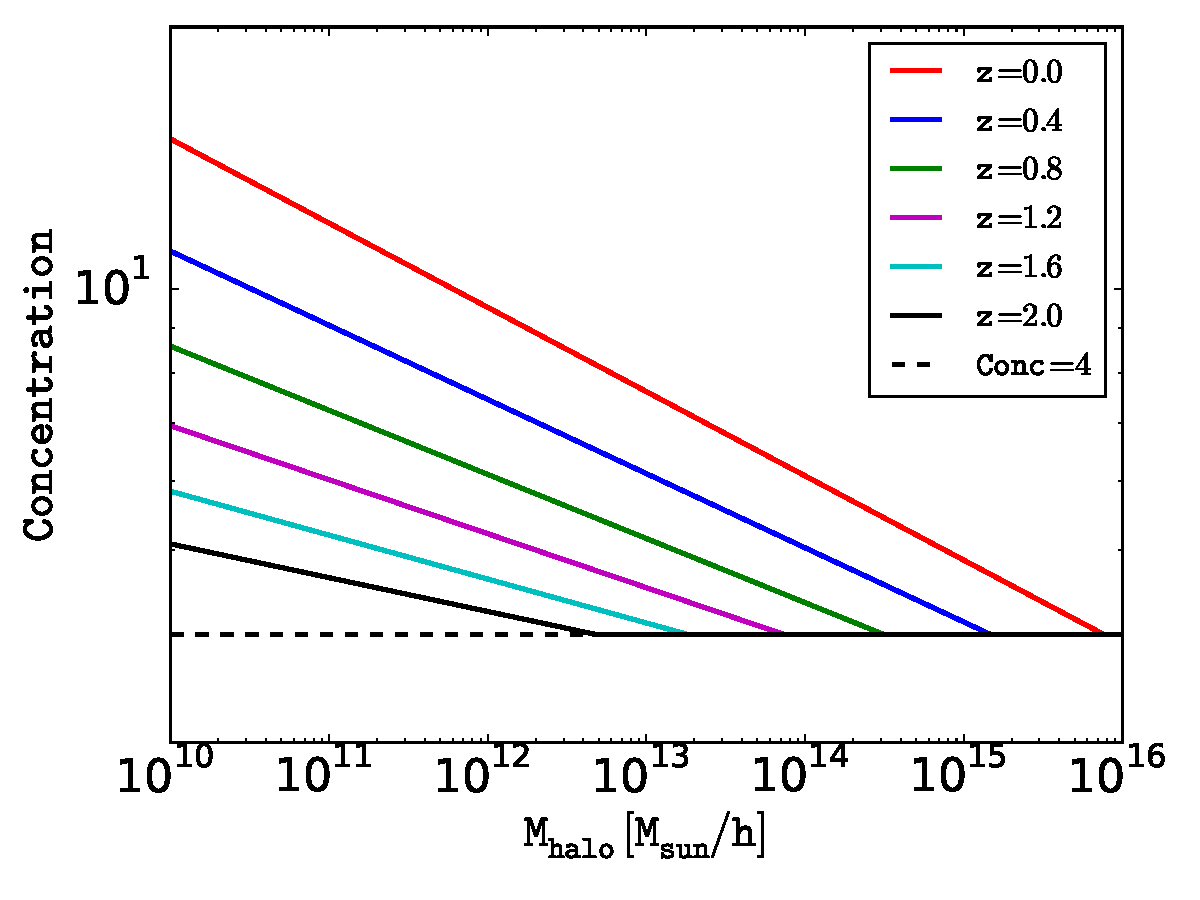
\includegraphics[width=0.48\linewidth]{figures/p3-figures/conc_mhalo.pdf}
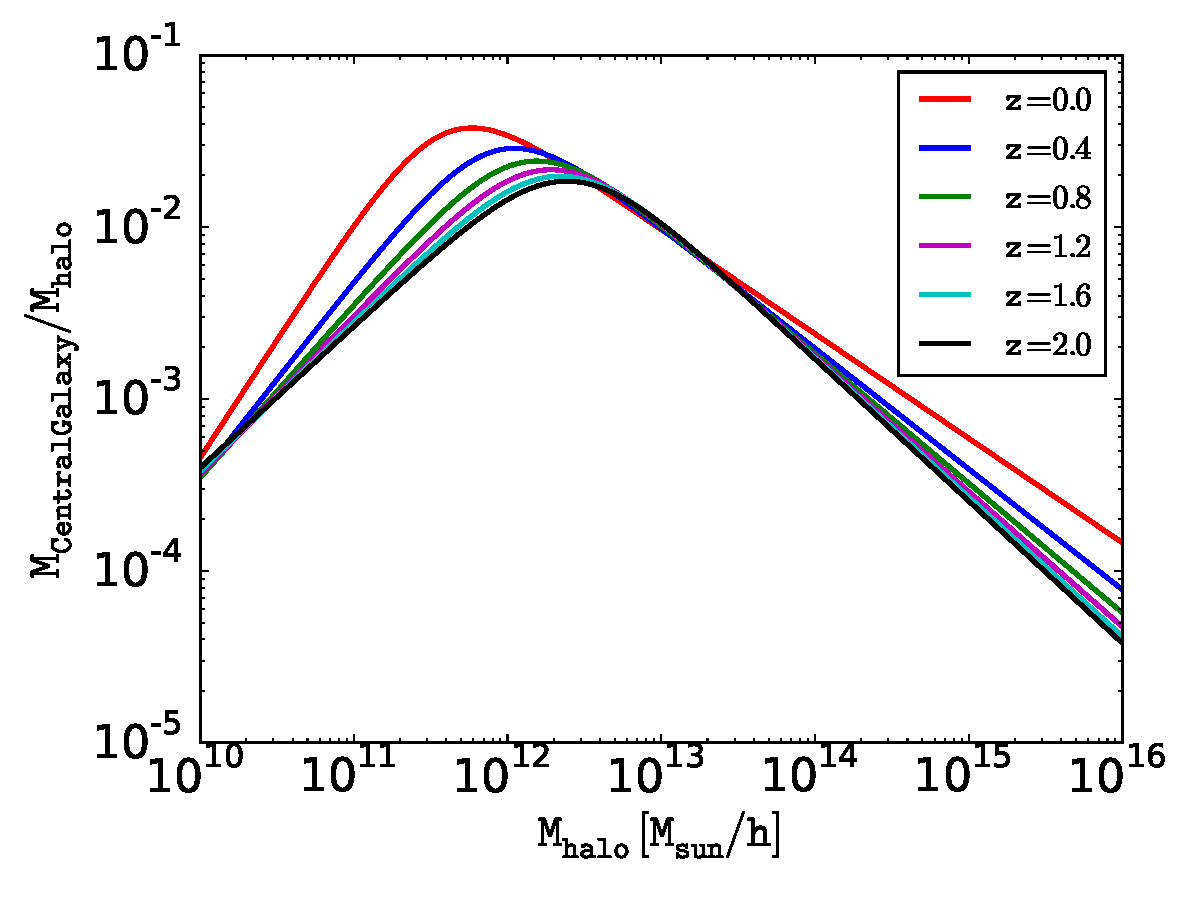
\includegraphics[width=0.48\linewidth]{figures/p3-figures/bcg_mhalo.pdf}
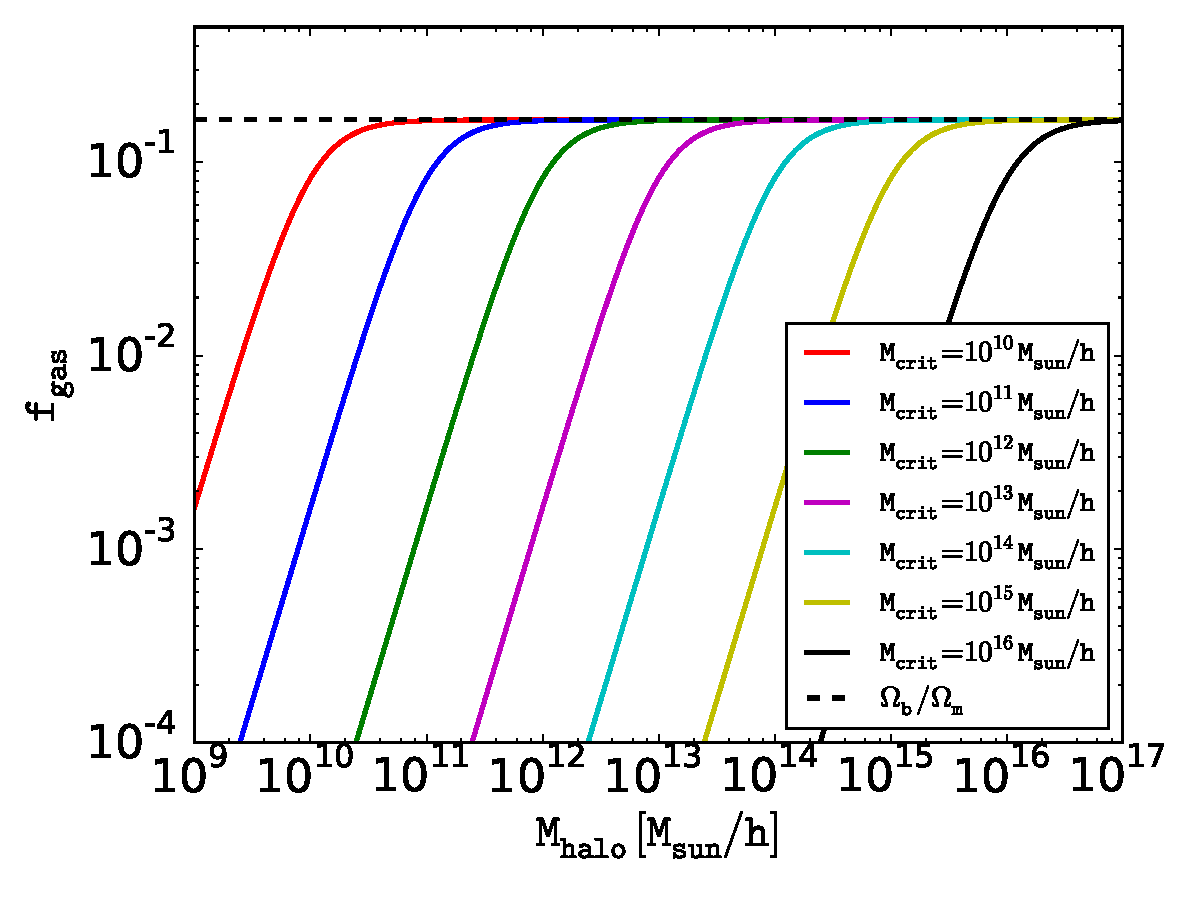
\includegraphics[width=0.48\linewidth]{figures/p3-figures/fgas_mhalo.pdf}
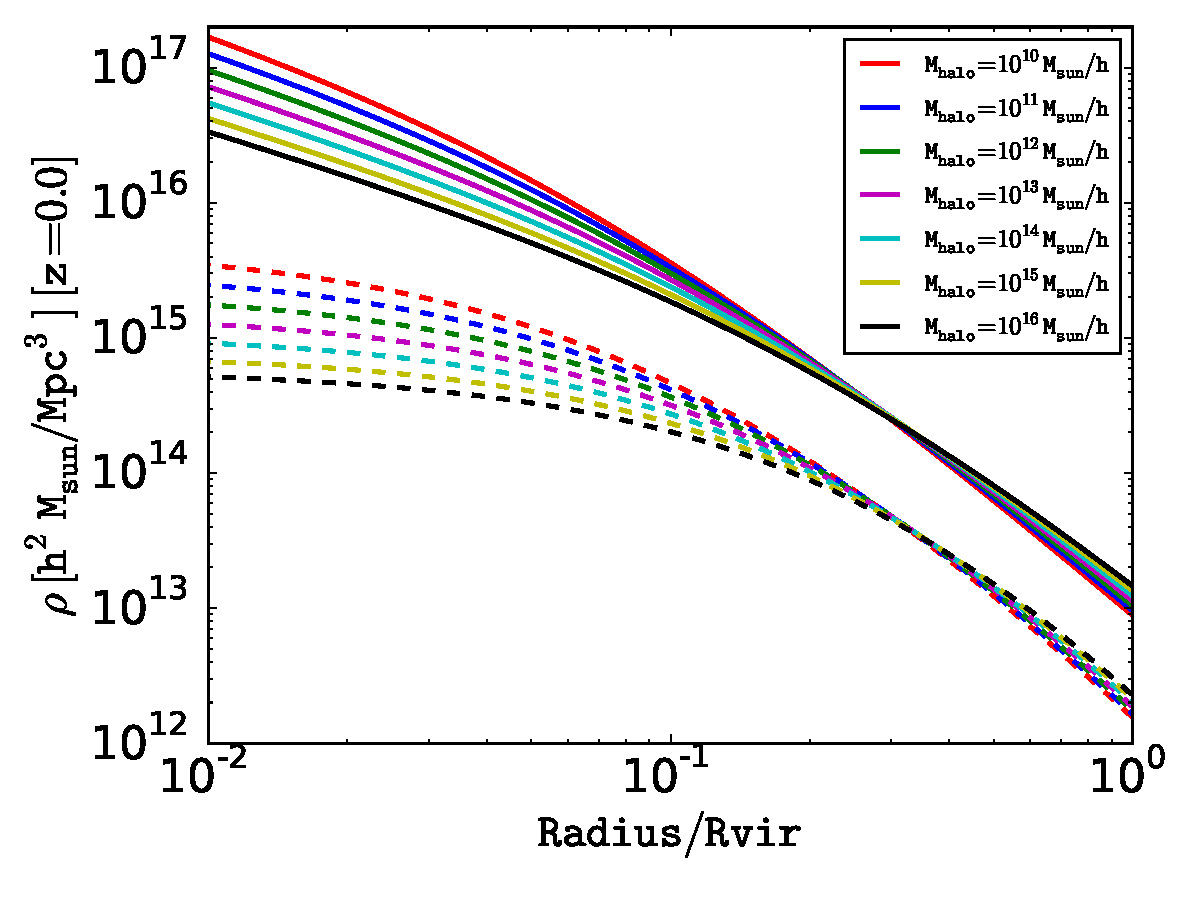
\includegraphics[width=0.48\linewidth]{figures/p3-figures/rho_nfw_gas_z0.pdf}
\caption{Top left: Concentration parameter as a function of halo mass for variable redshift. Top right: Mass of the central galaxy as a function of halo mass for variable redshift. Bottom left: Gas mass fraction as a function of halo mass for variable $M_{\rm crit}$. Bottom right: Density profile for NFW (solid lines) and intra-cluster gas (dashed lines) for different halo masses at redshift 0.}
\label{p3:fig:halo}
\end{figure}
\clearpage


We used the \cite{1998ApJ...496..605E, 1999ApJ...511....5E} transfer function calculations to account for the linear matter power spectrum term, $P_{lin}(k)$. The term $u(k|M)$ is the Fourier transform of the normalized density profile and is given by,

\begin{equation}
	u(k|M) = \dfrac{4 \pi}{M} \int_0^{R_{\rm vir}}dr\  r^2\  \rho(r|M)\ \dfrac{\sin(kr)}{kr}.
\end{equation}

where, $\rho(r|M)$ is the density profile of the halo of mass $M$. The function $u(k|M)$ is normalised such that $u(k=0|M)=1$ .The dispersion of the smoothed density field, $\sigma(M,z)$, is given by,
\begin{equation}
	\sigma^2(M,z) = \dfrac{1}{2 \pi^2} \int P_{\rm lin}(k) k^2 |\tilde{W}(R,k)|^2 dk,
\end{equation}

where, $\tilde{W}(R,k)$ is the Fourier transform of top-hat filtering function and given by,
\begin{equation}
	\tilde{W}(R,k) = 3 \dfrac{\textrm{sin}(kR) - kR \textrm{cos}(kR)}{(kR)^3}
\end{equation}

This framework of the halo model is applied to both DMO and BAR model which, differ in the halo density profiles and normalization of the mass function. The following two sections explains the corresponding profiles.

%----------------------------------------------------------------------
\subsection{Dark matter only}\label{p3:sec:darkmatteronly}
We started with the radial density profile of dark matter halos given by the functional form:
\begin{equation}
 \rho(r|M) = \dfrac{\rho_s}{(r/R_s)^\alpha (1+r/R_s)^\beta},
\end{equation}

where, $R_s$ is the characteristic radius given by the concentration parameter ($c$) and the virial radius of the halo ($r_{vir}$) as $c = R_{\rm vir}/R_s$. We used the two parameters $\alpha$ and $\beta$ to be 1 and 2 respectively, corresponding to the Navarro-Frenk-White (NFW) profile \citep{1997ApJ...490..493N}. The characteristic density $\rho_s$ which is strongly degenerate with $R_s$ and also proportional to the critical density of the Universe when the halo was formed. So, the NFW profile for dark matter halos is completely described by its concentration. 

The concentration parameter $c$ gives the information about the environment or the mean background density during the formation of the halo. A number of $N$-body simulations \citep{1997ApJ...490..493N, 1999MNRAS.310..527A, 2000ApJ...535...30J, 2001MNRAS.321..559B, 2001ApJ...554..114E, 2003ApJ...597L...9Z, 2007MNRAS.381.1450N, 2007MNRAS.378...55M, 2008MNRAS.390L..64D, 2008MNRAS.387..536G, 2014MNRAS.441.3359D} has prescribed various power laws between mass of the halo ($M$) and its concentration parameter $c$ at redshift $z$. We used the fitting formula given in \citep{2011MNRAS.411..584M}:

\begin{equation}
	\log(c) = a(z)\log(M_{\rm vir}/[h^{-1} M_{\bigodot}]) + b(z)
\end{equation}

where,
\begin{equation}
	a(z) = \omega z - m
\end{equation}

and
\begin{equation}
	b(z) = \dfrac{\alpha}{z+\gamma} + \dfrac{\beta}{(z+\gamma)^2}
\end{equation}

The fitting parameters $\omega,\ m,\ \alpha,\ \beta\ {\rm and}\ \gamma$ are 0.029, 0.097, -110.001, 2469.720 and 16.885 respectively.
Figure \ref{p3:fig:halo} (top-left panel) shows the behaviour of the concentration parameter as function of halo mass at different redshifts. There is an anti-correlation between the mass of the halo and its concentration. Also for a given halo mass, the concentration decreases with redshift. We limit the minimum concentration to 4 (dashed line in figure \ref{p3:fig:halo} upper-left panel). This is because the higher mass halos did not reach there maximum formation efficiency redshift and will reach it in future. So, on an average, there concentration must not be less than a few. A very recent study from \cite{2014MNRAS.441.3359D} shows that this behaviour is consistent and the minimum concentration is very close to 4. 

%----------------------------------------------------------------------

\subsection{A baryonic model}\label{p3:sec:baryonicmodel}
Our baryonic model accounts within each halo for: 1) a central galaxy, the major stellar component whose properties are derived from abundance matching techniques; 2) a hot plasma in hydrostatic equilibrium and 3) an adiabatically-contracted (AC) dark matter component. This analytic approach allows us to compare our model to the DMO case. Apart from the normalization of the mass function, there is only one term that is affected by these baryonic components and is the density profile of the halo, which no longer follows the NFW profile. We can write the modified NFW (BAR) profile as:
\begin{equation}
	\rho_{\rm BAR}(r|M) = f_{\rm dm}\rho_{\rm NFW}^{\rm AC}(r) + \rho_{\rm BCG}(r) + f_{\rm gas}(M)\rho_{\rm gas}(r),
\end{equation}

we discuss each of these terms in more details.

%-------------------------------------------------------------------------

\subsubsection{Stellar component}\label{p3:sec:stellar}
We used the fitting function from \cite{2013MNRAS.428.3121M} based on abundance matching to map the stellar mass of the central galaxy $M_{\rm CentralGalaxy}$ (BCG), which is the major component of stellar mass in a cluster, to the mass of the halo ($M_{\rm{halo}}$). Figure \ref{p3:fig:halo} (top-right panel) shows the mapping between halo mass and stellar mass fraction associated to the central galaxy for a variety of redshifts. The relation has a positive slope for low mass halos, however, at about the size of the Milky way halo, the slope turns negative. At this peak, the central galaxy stellar mass contributes about 4-5 $\%$ of the total mass of the halo. Also this peak shifts to higher masses for higher redshifts but contributes lower fraction. 

The actual distribution of stellar mass in galaxy groups and clusters can be quite complex. The total stellar mass budget can be decomposed in 3 components: satellite galaxies, Brightest Cluster Galaxy (BCG, the massive elliptical galaxy dominating the cluster centre) and Intra-cluster Light (ICL, an extended stellar halo surrounding the BCG). The BCG and ICL represent $\sim 40$ \% of the mass in clusters, with this ratio decreasing with total cluster mass \citep{2007ApJ...666..147G}. However, BCG+ICL dominate the inner part of the cluster and constitute $\sim 70\%$ of the total stellar mass within 0.1 $R_{200}$. This fact is particularly relevant for computing the effect of baryon condensation on the dark matter profiles (see Subsection \ref{p3:sec:adcon}). The BCG+ICL component is usually modelled using superimposition of fitting functions, typically multiple Sersic profiles. Given that we are not interested in detailed modelling of the stellar distribution, we consider a simplified model for the BCG+ICL. 


we adopted a radial density profile for BCG, where the enclosed mass  goes linearly with the radius, 
\begin{equation}
	M_{\star}(<r) = M_{\rm CentralGalaxy} \dfrac{r}{2R_{1/2}}
\end{equation}

this gives,
\begin{equation}
	\rho(r) = \dfrac{M_{\rm CentralGalaxy}}{8 \pi R_{1/2} r^2},\ r<2R_{1/2}
\end{equation}

where, $R_{1/2}$ is the half mass radius. We use $R_{1/2} = 0.015 R_{\rm vir}$ which is a good fit to the observations \citep{2014arXiv1401.7329K}. We forced the density profile to drop exponentially after $2R_{1/2}$.


%We assume a Gaussian profile for the BCG which is normalized to its mass from the abundance matching relation ($M_{\rm{CentralGalaxy}}$) concentrated at the centre of the cluster.  Nearly all the mass of the BCG for most of the clusters is concentrated with a radius of 50 kpc. The concentration or the extent of this galaxy can be controlled with the Gaussian width, which is fixed to 5 kpc in this work. 

%-------------------------------------------------------------------------

\subsubsection{Intra-cluster plasma}\label{p3:sec:gas}
\label{p3:sec:icm}

The major component of the baryonic matter in a galaxy cluster is the hot intra-cluster gas. It is mainly ionized hydrogen at very high temperature and low density. This plasma radiates in X-rays and can safely be assumed to be in hydrostatic equilibrium. We assume this gas distribution in the halo according the hydrostatic equilibrium equations given in \cite{2013MNRAS.432.1947M},

\begin{equation}
	\rho(x) = \rho_0 \left[\dfrac{\ln(1+x)}{x}  \right]^{\dfrac{1}{\Gamma -1}}
\end{equation}

where, $x$ is the distance from the centre of the halo in unit of scale radius $R_s$. The effective polytropic index $\Gamma$ is given by,

\begin{equation}
	\Gamma = 1+ \dfrac{(1+x_{eq})\ln(1+x_{eq}) - x_{eq}}{(1+3x_{eq})\ln(1+x_{eq})}
\end{equation}

where, $x_{eq}=c/\sqrt{5}$. Figure \ref{p3:fig:halo} (bottom-right in dashed lines) shows the density profile of the hot gas for variable halo masses at redshift 0 and also shows the comparison to the NFW profile (solid lines). For $x>x_{eq}$, the gas density profiles follows the NFW profile, however, it approaches a nearly constant values near the centre of the halo. 

The normalization of the gas density profile, $\rho_0$, is fixed by the gas fraction $f_{\rm{gas}}$. if we assume no feedback from the baryonic component of the halo, this number can be a constant, however, many hydrodynamical simulations \citep{2005MNRAS.356..107R, 2005MNRAS.360..892D, 2006Natur.442..539M, 2012MNRAS.421.3464P, 2013MNRAS.429.3068T, 2013MNRAS.432.1947M} shows signatures of the expulsion of gas from the halo. This expulsion is stronger in low mass halos than the high mass halos. So the low mass halos are generally deficit in this hot plasma component. Following the same physical motivation, we used the gas mass fraction of the halo to be the function of the mass of the halo following the parametric form:
\begin{equation}
	f_{\rm{gas}}(M_{\rm halo}) =  \dfrac{\Omega_b/\Omega_m}{1 + \left (\dfrac{M_{\rm{crit}}}{M_{\rm{halo}}} \right) ^{\beta}}
\end{equation}

where, $M_{\rm{crit}}$ is a free parameter and $\beta$ is fixed to 2. This parameter controls the gas fraction in halos of different mass. A higher value for $M_{\rm{crit}}$ represents less gas in the halo up to higher halo masses. This parameter can also be interpreted as the control sequence for AGN feedback. Figure \ref{p3:fig:halo} (bottom-left panel) shows the variation of $f_{\rm{gas}}$ with halo mass for variety of $M_{\rm{crit}}$. We chose $M_{\rm crit} = 10^{13} h^{-1} M_{\bigodot}$ as the most realistic model. In this case, all halos with mass lower than $\sim 2\times 10^{12} h^{-1} M_{\bigodot}$ have expelled all their gas to the background (outside the $R_{\rm vir}$) and all halos with mass larger than $\sim 2\times 10^{13} h^{-1} M_{\bigodot}$ have all their gas inside the halo. The intermediate mass halos have a very smooth transition from no gas to all gas inside the halo. This behaviour matches well with recent study from \cite{2014arXiv1409.8617S}. We studied this case in detail for all its cosmological implications at different scales. We also studied one optimistic\footnote{Optimistic in the sense of less AGN feedback that makes the baryonic corrections less troublesome} model, where the feedback is not as strong as in our realistic model, with $M_{\rm crit} = 10^{12} h^{-1} M_{\bigodot}$.


%-------------------------------------------------------------------------

\subsubsection{Adiabatic contraction}\label{p3:sec:ac}
\label{p3:sec:adcon}
In the DMO model, we adopted the NFW profile for the distribution of dark matter in the halo which is nearly scale-free and completely described by the concentration parameter. However, in the presence of baryons, the dark matter component follows NFW only in the outskirts of the halo, but in the very centre the dark matter profile becomes steeper and deviates from pure a NFW profile.  This is because the baryons, which are dominant in the centre of the halo, drag some extra matter from the surrounding towards the centre making the dark matter profile steeper towards the centre. The total distribution of matter is expected to dynamically respond to the condensation of baryons at the centre of the halo in a way that approximately conserves the value the adiabatic ``invariant'' $R\times M(R)$, where $R$ is the distance from the halo centre and $M(R)$ is the mass enclosed in a sphere of radius R \citep{1986ApJ...301...27B, 2004ApJ...616...16G}. We adopted a simplified model for this effect following the appendix of \cite{2011MNRAS.414..195T} where this adiabatic contraction (AC) of the dark matter profile is solely governed by the central galactic disk. 


%----------------------------------------------------------------------



\subsection{Comparison with simulations}\label{p3:sec:simulations}

\begin{figure}[p]
\centering
	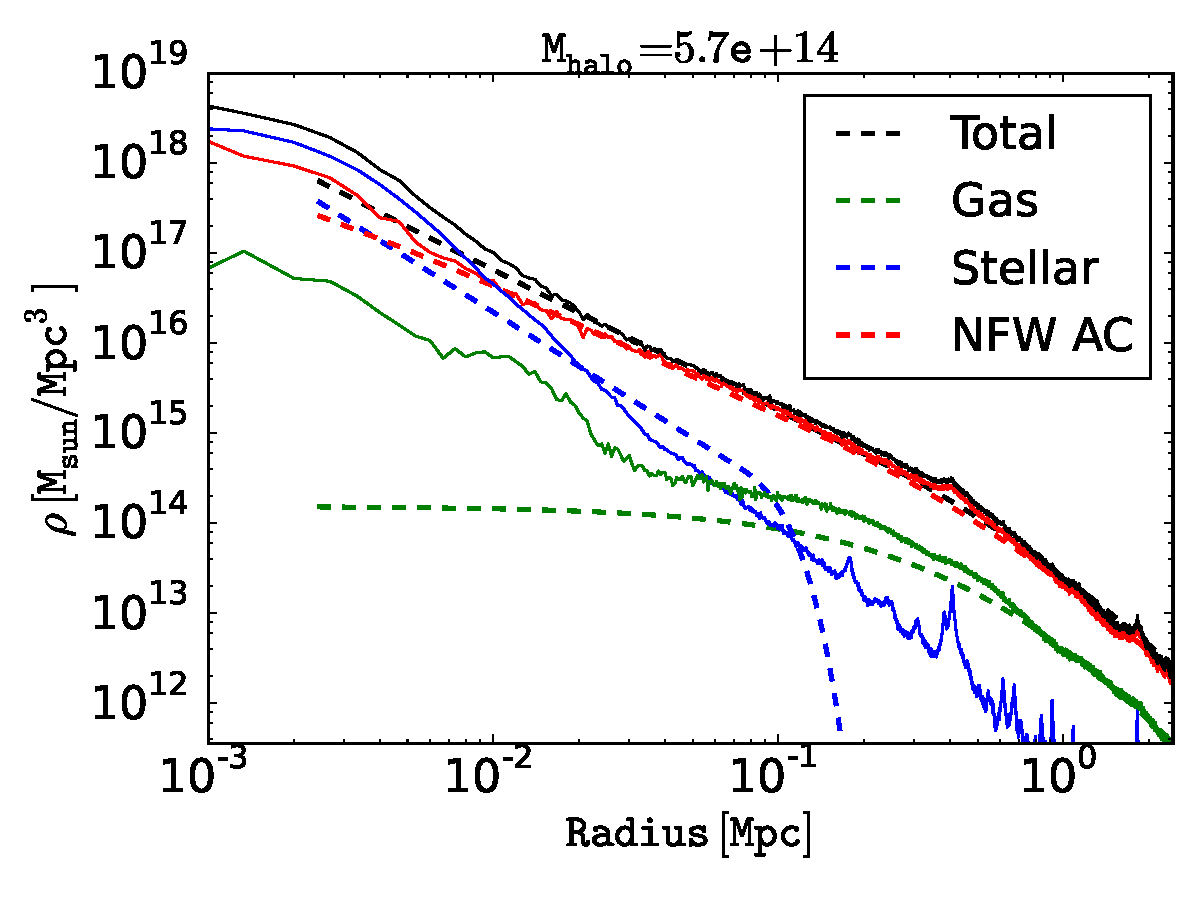
\includegraphics[width=0.48\linewidth]{figures/p3-figures/AGN00001.pdf}
	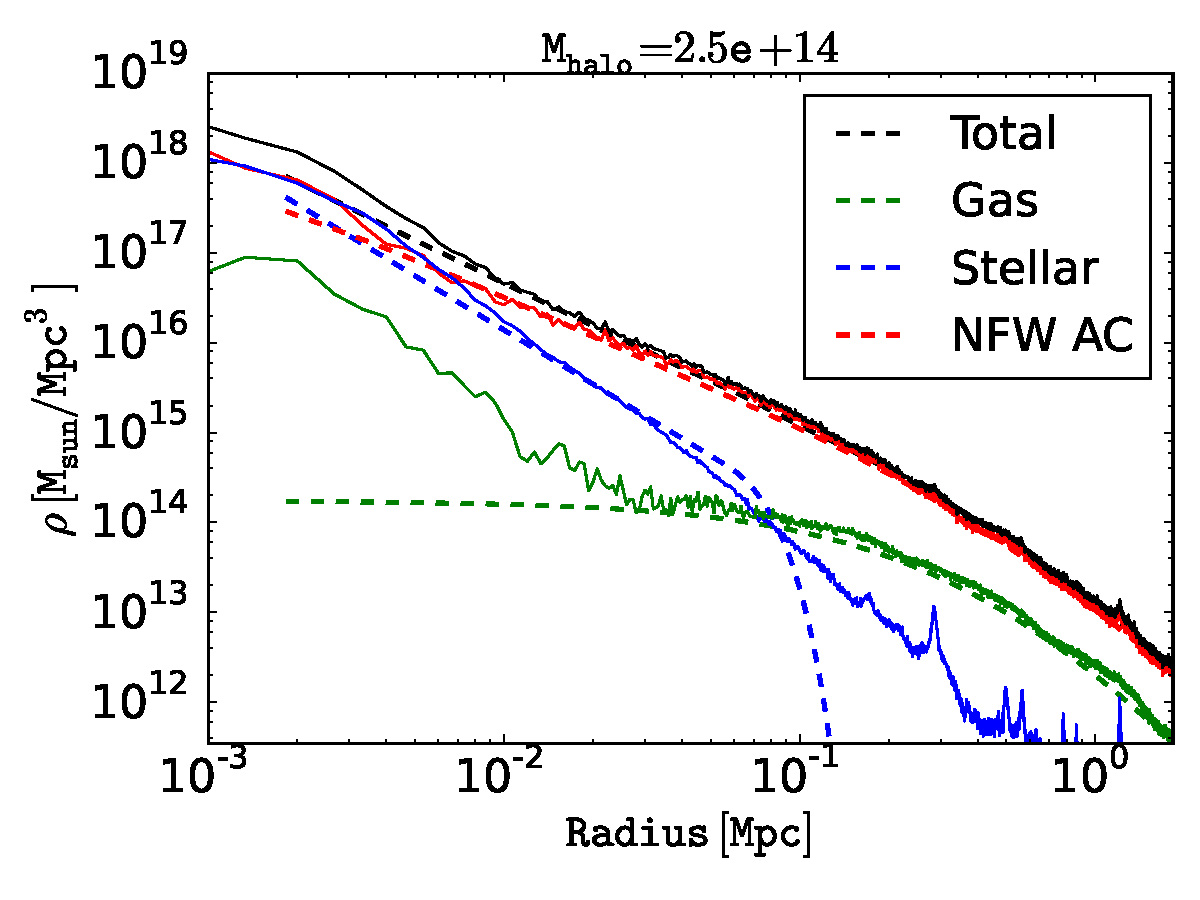
\includegraphics[width=0.48\linewidth]{figures/p3-figures/AGN00003.pdf}
	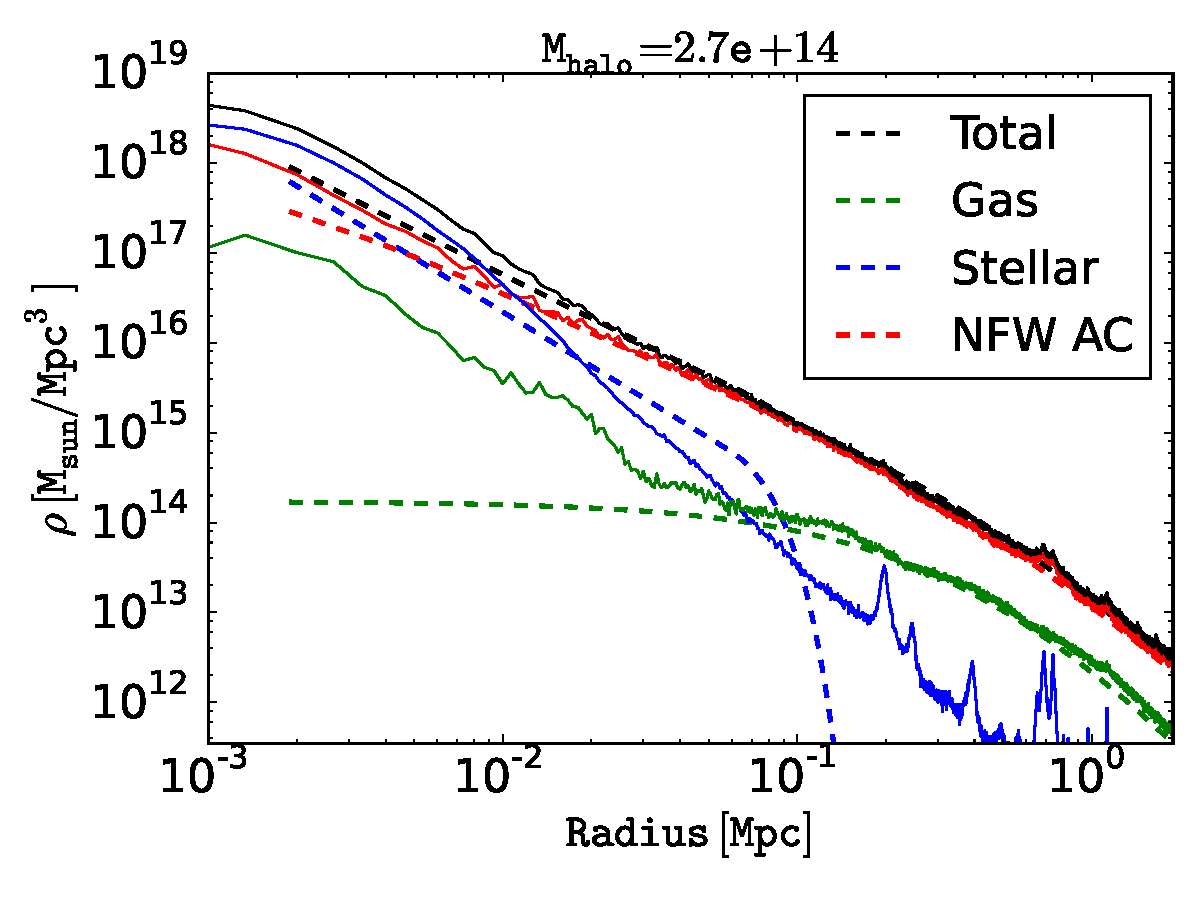
\includegraphics[width=0.48\linewidth]{figures/p3-figures/AGN00004.pdf}
	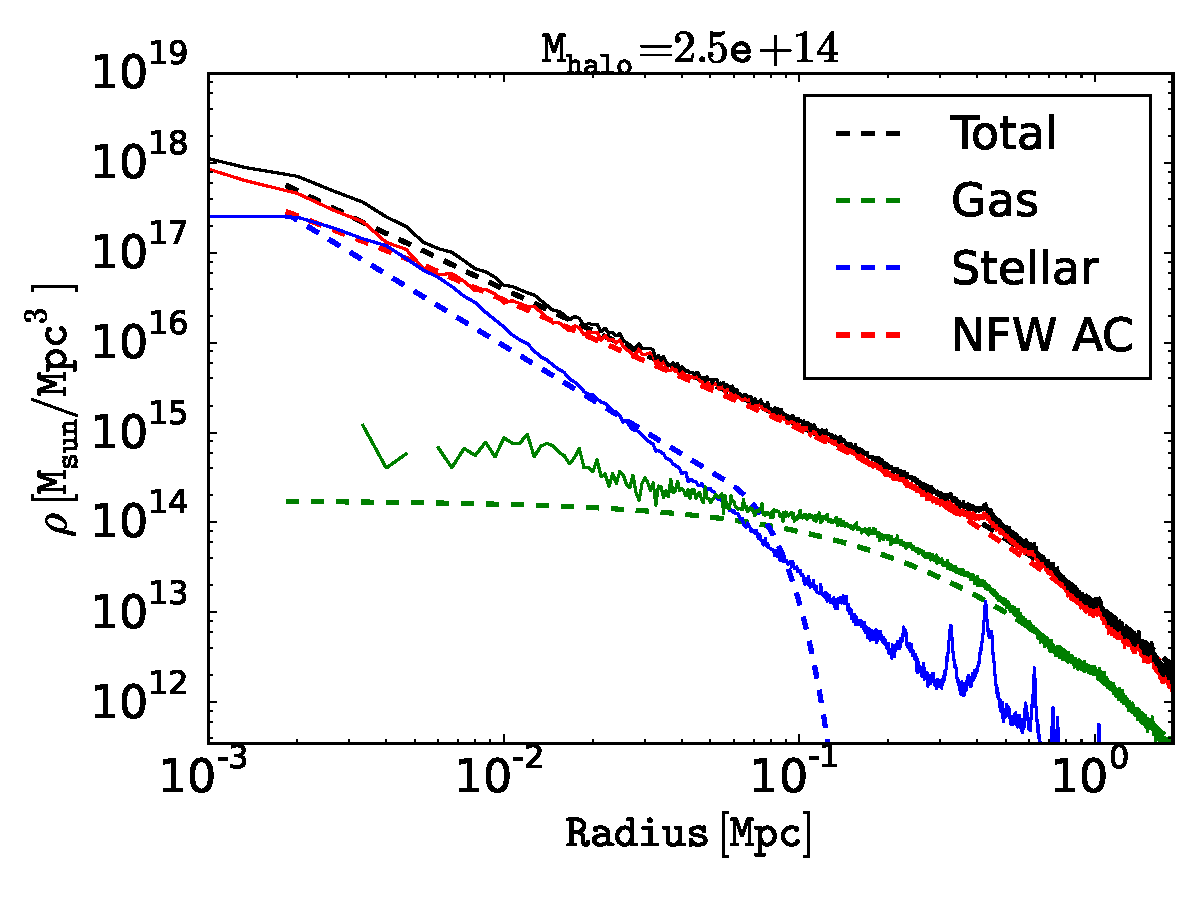
\includegraphics[width=0.48\linewidth]{figures/p3-figures/AGN00005.pdf}
	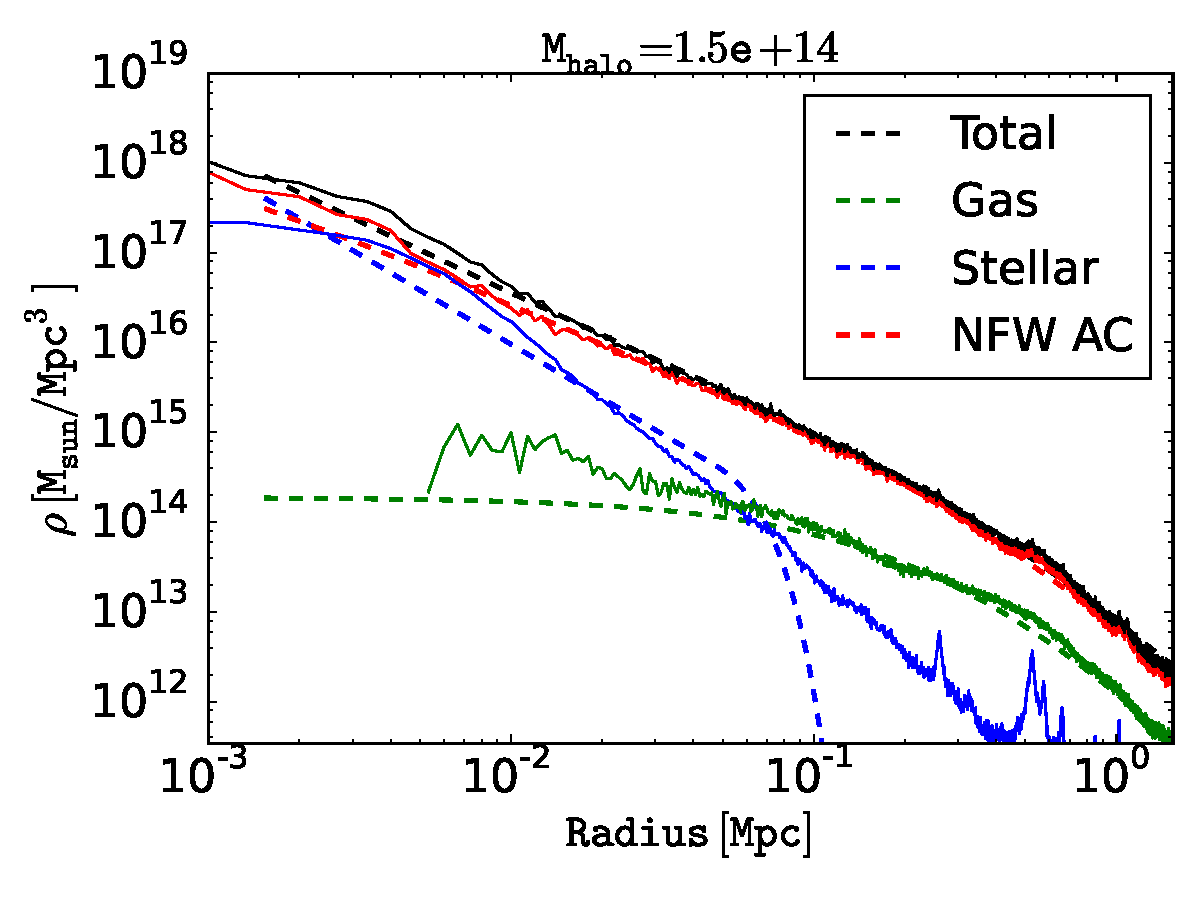
\includegraphics[width=0.48\linewidth]{figures/p3-figures/AGN00006.pdf}
	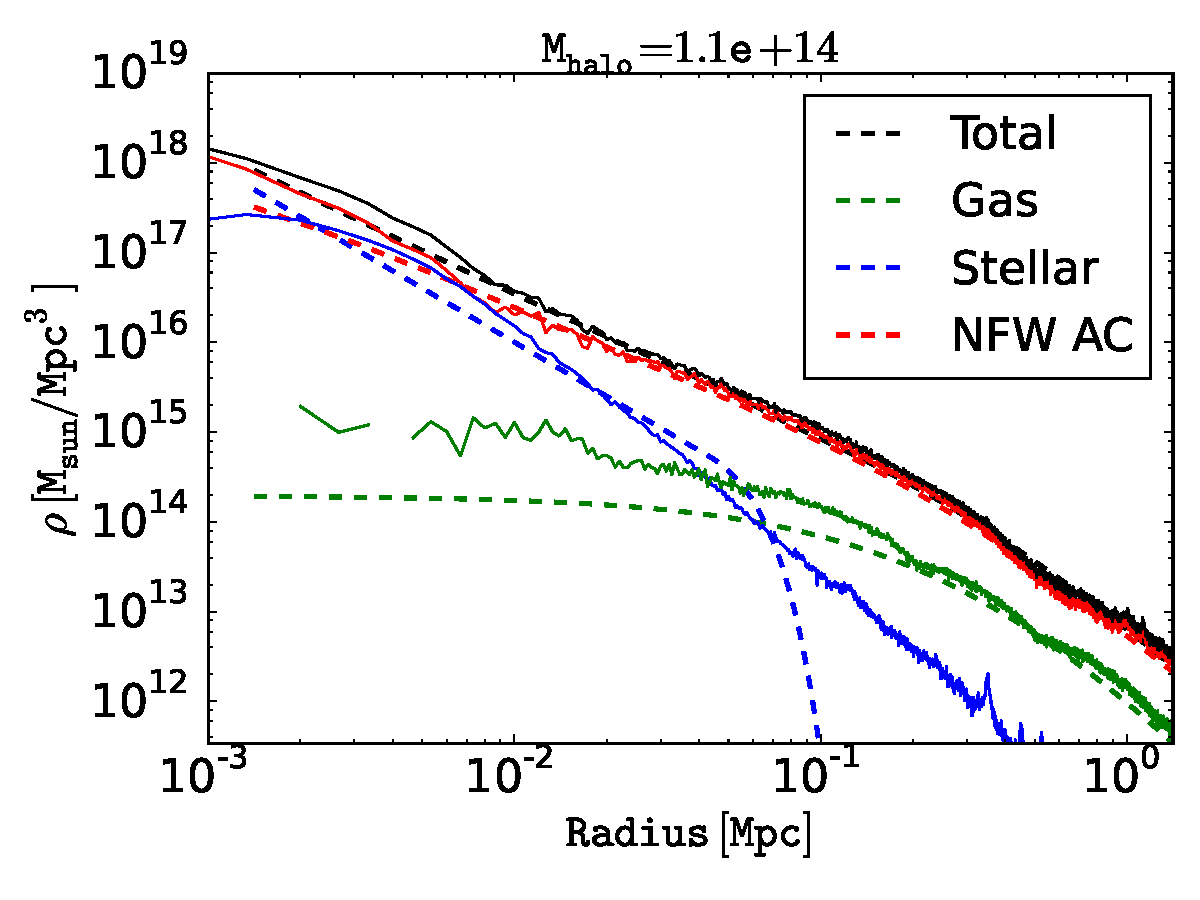
\includegraphics[width=0.48\linewidth]{figures/p3-figures/AGN00008.pdf}
	\caption{A comparison of our model density profiles (dashed lines) with hydrodynamical simulations of Martizzi et. al. 2014 (solid lines). There is a remarkable agreement, except at the very centre of the halo.}
	\label{p3:fig:compare}
\end{figure}
\clearpage

\begin{table}[p]
\centering
\begin{tabular}{|l|c|c|c|c|c|c|}
\hline
\hline
 Type & $H_0$ & $\sigma_{\rm 8}$ & $n_{\rm s} $ & $\Omega_\Lambda$ & $\Omega_{\rm m}$ & $\Omega_{\rm b}$ \\
\hline
\hline
DMO & 70.4 & 0.809 & 0.963 & 0.728 & 0.272 & - \\
BAR & 70.4 & 0.809 & 0.963 & 0.728 & 0.272 & 0.045 \\
\hline
\hline
\end{tabular}
\caption{Cosmological parameters adopted in our simulations. }\label{p3:tab:cosm_par}
\end{table}

\begin{table}[p]
\centering
\begin{tabular}{|l|c|c|c|}
\hline
\hline
{\itshape Type} & $m_{\rm cdm}$&  $m_{\rm gas}$ & $\Delta x_{\rm min}$ \\
 & $[10^{8}$ M$_\odot$/h] & $[10^{7}$ M$_\odot$/h] & [kpc/h] \\
\hline
\hline      
 Original box & $ 15.5 $ & n.a. & $2.14$ \\
 DMO zoom-in & $1.94$ & n.a. & $1.07$ \\
 BAR zoom-in & $1.62$ & $3.22$ & $1.07$ \\
\hline
\hline
\end{tabular}
\caption{Mass resolution for dark matter particles, gas cells and star particles, and spatial resolution (in physical units) for our simulations. }\label{p3:tab:mass_par}
\end{table}

We consider data from a set of cosmological re-simulations performed with the {\scshape ramses} code \cite{2002A&A...385..337T}. These simulations are part of a larger set recently used 
by \cite{2014MNRAS.440.2290M} to study the baryonic effects on the halo mass function. Thanks to the adaptive mesh refinement capability of the {\scshape ramses} code, the resolution 
achieved in these simulations is sufficient to study the properties of low redshift BCGs. 

In these calculations, the cosmological parameters are: matter density parameter $\Omega_{\rm m}=0.272$, cosmological constant density parameter $\Omega_\Lambda=0.728$, baryonic matter 
density parameter $\Omega_{\rm b}=0.045$, power spectrum normalization $\sigma_{\rm 8}=0.809$, primordial power spectrum index $n_{\rm s}=0.963 $ and Hubble constant $H_0=70.4$ km/s/Mpc 
(Table~\ref{p3:tab:cosm_par}). We generated initial conditions for the simulations using the \cite{1998ApJ...496..605E} transfer function and the {\scshape grafic++} code\footnote{http://sourceforge.net/projects/grafic/}, based on the original {\scshape grafic} code \citep{2001ApJS..137....1B}. These simulations come in two flavours: DMO (dark matter only) 
which only follow the evolution of dark matter, BAR which include baryons and galaxy formation prescriptions. 

The technique we adopted to perform the zoom-ins is described in the following. First, we ran a dark matter only simulation with particle mass $m_{\rm cdm}=1.55\times 10^9$~M$_\odot$/h 
and box size $144$~Mpc/h. The initial level of refinement was $\ell=9$ ($512^3$), but as the simulation evolved more levels of refinement were allowed. At redshift $z=0$ the grid was 
refined down to a maximum level $\ell_{\rm max}=16$. Subsequently, we ran apply the AdaptaHOP algorithm \cite{2004MNRAS.352..376A} to identify the position and masses of dark 
matter halos. We selected 51 halos whose {\it total} masses lie $M_{\rm tot}>10^{14}$~M$_\odot$ and whose neighbouring halos do not have masses larger than $M/2$ within a spherical 
region of five times their virial radius. We determined that only 25 of these clusters are relaxed. High resolution initial conditions were extracted for each of the 51 halos and were used 
to run zoom-in re-simulations. Three different re-simulations per halo have been performed: (I) including dark matter and neglecting baryons, (II) including dark matter, baryons 
and stellar feedback, (III) including baryons, stellar feedback and AGN feedback. In this paper we focus on cases (I) and (III), labelled DMO and BAR, respectively.

In the DMO re-simulation, the dark matter particle mass is $m_{\rm cdm}=1.94\times 10^{8}$~M$_\odot$/h. In the BAR re-simulations, the dark matter particle mass is 
$m_{\rm cdm}=1.62\times 10^{8}$~M$_\odot$/h, while the baryon resolution element has a mass of $m_{\rm gas}=3.22\times 10^{7}$~M$_\odot$. The maximum refinement level was set to $\ell=17$, 
corresponding to a minimum cell size $\Delta x_{\rm min} = L/2^{\ell_{\rm max}}\simeq 1.07$ kpc/h. The grid was dynamically refined using a quasi-Lagrangian approach: 
when the dark matter or baryonic mass in a cell reaches 8 times the initial mass resolution, it is split into 8 children cells. Table~\ref{p3:tab:mass_par} summarizes the particle mass and 
spatial resolution achieved in the simulations.

The physical prescription implemented in the code to perform the BAR simulations is here briefly described. In {\scshape ramses} gas dynamics is solved via a second-order unsplit Godunov 
scheme \citep{2002A&A...385..337T} based on different Riemann solvers (we adopted the HLLC solver) and the MinMod slope limiter. The gas is described by perfect gas equation of state 
(EOS) with polytropic index $\gamma=5/3$. Gas cooling is modelled with the \cite{1993ApJS...88..253S} cooling function which accounts for H, He and metals. Star formation and supernovae 
feedback ("delayed cooling" scheme, \cite{2006MNRAS.373.1074S}) and metal enrichment have been included in the calculations. AGN feedback has been included too, using a method inspired by 
the \cite{2009MNRAS.398...53B} model. In this scheme, super-massive black holes (SMBHs) are modeled as sink particles and AGN feedback is provided in form of thermal energy injected in a 
sphere surrounding each SMBH. More details about the AGN feedback scheme and about the tuning of the galaxy formation prescriptions can be found in \cite{2011MNRAS.414..195T} and \cite{2012MNRAS.422.3081M}.




Figure~\ref{p3:fig:compare} shows the comparison between the dark matter, gas, stellar and total mass density profiles of 6 halos in the \cite{2014MNRAS.440.2290M} catalogue and the mass model described in Section \ref{p3:sec:halomodel}. The model for the adiabatically contracted dark matter profile (red dashed lines) fits well the simulations down to scales $\sim 10$ kpc. The model for the Intra-cluster plasma (green dashed lines) fits well the results of the simulations down to scales $\sim 50$ kpc. The relation between mass of the central galaxy and that of the halo has a lot of scatter. So, to compare with simulations we use the stellar mass from the simulation itself for the given halo, which define the normalisation of our stellar model. The model (blue dashed lines) is a good fit to the results of the simulations except in the outskirts. This is expected since the data from the simulations include BCG, ICL and satellite galaxies. However, the model is constructed in such a way that the stellar mass expected from abundance matching is associated to the central regions of the halos. The overall result is that the model for the total mass (black dashed lines) provides an excellent match to the results of cosmological simulations down to a scale of $\sim 10$ kpc. Therefore we conclude that the mass model is good enough to be adopted for the purposes of this paper.


%===============================================================================


\subsection{From \texorpdfstring{$P(k)$}{P(k)} to \texorpdfstring{$C(\ell)$}{C(ell)}}
\label{p3:sec:pk2cl}
In this section we develop the mapping from 3D matter power spectrum $P(k,z)$ to the 2D projected shear angular power spectrum $C_{\ell}$ following the theoretical framework explained in \cite{2009MNRAS.395.2065T}.

The distortion of the source shape due to weak gravitational lensing can be quantified with two quantities: shear $\gamma$ and convergence $\kappa$. The convergence $\kappa$ is the local isotropic part of the deformation matrix and can be expressed as:
\begin{equation}
	\kappa(\vec{\theta}) = \dfrac{1}{2} \vec{\bigtriangledown}.\vec{\alpha}(\vec{\theta})
\end{equation}

where, $\alpha$ is the deflection angle. If we know the redshift of the source galaxies, additional information can be gained by dividing the sources in different redshift bins. This process is referred to as lensing tomography and is very useful to gain extra constraints on cosmology from the evolution of the weak lensing power spectrum \citep{1999ApJ...522L..21H, 2002PhRvD..65f3001H, 2004MNRAS.348..897T}. In cosmological context, the convergence field can be expressed as the weighted projection of the mass distribution integrated along the line of sight in the $i$th redshift bin, 

\begin{equation}
	\kappa_i(\vec{\theta}) =  \int_0^{\chi_H} g_i(\chi) \delta(\chi \vec{\theta},\chi)d\chi,
\end{equation}

where, $\delta$ is the total 3 dimensional matter overdensity, $\chi$ is the comoving distance and $\chi_H$ is the comoving distance to the horizon. For a complete review see \cite{1999ARA&A..37..127M, 2001PhR...340..291B, 2006glsw.conf..269S}. The lensing weights $g_i(\chi)$ in the $i$th redshift bin with comoving distance range between $\chi_i$ and $\chi_{i+1}$ are given by:

\begin{equation}
g_i(\chi) = \begin{cases} \dfrac{g_0}{\bar{n}_i} \dfrac{\chi}{a(\chi)} \int_{\chi_i}^{\chi_{i+1}} n_s(\chi^{\prime})\dfrac{dz}{d\chi^{\prime}} \dfrac{(\chi^{\prime} - \chi) }{\chi^{\prime}} d\chi^{\prime}, & \chi \le \chi_{i+1} \\
			0, & \chi > \chi_{i+1} \end{cases}
\end{equation}

where, $a(\chi)$ is the scale factor at comoving distance $\chi$. Also, 

\begin{equation}
	g_0 = \dfrac{3}{2} \dfrac{\Omega_m}{H_0^2}
\end{equation}

and,
\begin{equation}
	\bar{n}_i = \int_{\chi_i}^{\chi_{i+1}} n_s(\chi(z)) \dfrac{dz}{d\chi^{\prime}} d\chi^{\prime}.
\end{equation}

where, $n_s(\chi(z))$ is the distribution of sources in redshift. We assume a source distribution along the line of sight of the form:
\begin{equation}
	n_s(z) = n_0 \times 4z^2 \exp\left(-\dfrac{z}{z_0}   \right)
\end{equation}

with $n_0 = 1.18 \times 10^{9} $ per unit steradian and $z_0$ is fixed such that the corresponding projected source density $n_g$ resembles the experiment, like Euclid etc.

\begin{equation}
	\int_0^{\infty} n_s(z)dz = \bar{n}_g.
\end{equation}

For Euclid like survey, we choose $z_0$ such that $\bar{n}_g=50$ sources per arcmin$^{-2}$ \citep{2008ARNPS..58...99H}.


Finally the shear power spectrum between redshift bins $i$ and $j$ can be computed as:

\begin{equation}
	C_{ij}(\ell) =  \int_0^{\chi_H} \dfrac{g_i(\chi) g_j(\chi)}{ \chi^2} P\left(\dfrac{\ell}{\chi},\chi \right)d \chi
\end{equation}

where, $P$ is the 3D matter power spectrum calculated using the halo model framework as described in section \ref{p3:sec:halomodel}. Larger $\ell$ corresponds to the smaller scale and the large contribution of $C_{\ell}$ at higher $\ell$ comes from non-linear clustering. 

We divided the big cosmological volume into 3 redshift bins with boundaries: 0.01, 0.8, 1.5 and 4.0; so we calculated total 6 convergence cross-spectra (3 auto-spectra and 3 cross-spectra).

The auto-spectra is contaminated by the intrinsic ellipticity noise and assuming its distribution to be completely uncorrelated to different source galaxies, the observed power spectrum $C_{ij}^{\rm{obs}}(\ell)$ is given by,

\begin{equation}
	C_{ij}^{\rm{obs}}(\ell) = C_{ij}(\ell) + \delta_{ij}\dfrac{\sigma_{\epsilon}^2}{\bar{n}_i},
\end{equation}

we choose $\sigma_{\epsilon}=0.33$ which is the RMS intrinsic ellipticity. The cross spectra is not contaminated by shot noise. 

The covariance matrix of $C_{\ell}$ has two contributions: Gaussian and non-Gaussian (NG). In this work we only consider the Gaussian contribution to the covariance matrix which is given by the following expression,
%\begin{equation}
\begin{align}
	{\rm Cov}_{ij,mn}(\ell,\ell^{\prime})& = \dfrac{\delta_{\ell\ell^{\prime}}}
										{\Delta\ell(2\ell+1) \rm{f_{sky}}} \times  \nonumber\\
										&\qquad  \left(C_{im}^{\rm{obs}}(\ell)C_{jn}^{\rm{obs}}(\ell)+
										C_{in}^{\rm{obs}}(\ell)C_{jm}^{\rm{obs}}(\ell) \right),
\end{align}
%\end{equation}

where, $\Delta\ell$ is the bin width of the $\ell$ and $f_{sky}$ is the sky fraction for the targeted experiment. This term is dominated by cosmic variance for lower $\ell$ and shot noise for higher $\ell$, however, for large number of sources, as in case of Euclid, and larger size of bins $(\Delta \ell)$ towards higher end of $\ell$, the shot noise can be significantly reduced.

The NG contribution to the covariance matrix of $C_{\ell}$ is rather complicated to calculate. It gives the correlation between different $\ell$. At the matter power spectrum level, this term depends on the matter trispectrum. To compute the NG covariance to lensing, we need to integrate the trispectrum in redshift and angle on the sky and then compute this quantity for various $\ell$ and $\ell^{\prime}$. So this is a 4D calculation of trispectrum which is computationally very expensive. \cite{2012PhRvD..86h3504Y} shows that these NG correction to the covariance becomes significant for $\ell$ of few thousand and \cite{2002PhR...372....1C} shows that neglecting this will introduce the bias in the cosmological parameters up to 20 $\%$. In this work, we are not taking into account these corrections and we are doing our analysis for different $\ell_{max}$: 1000, 2000, 3000, 4000, 5000, 6000, 8000, 10000 and 20000. We will discuss more about the NG covariance in section \ref{p3:sec:NG}. 
%----------------------------------------------------------------------

%===============================================================================

\section{Comparing BAR and DMO model}
\label{p3:sec:comparison}

\begin{figure}[p]
\centering
	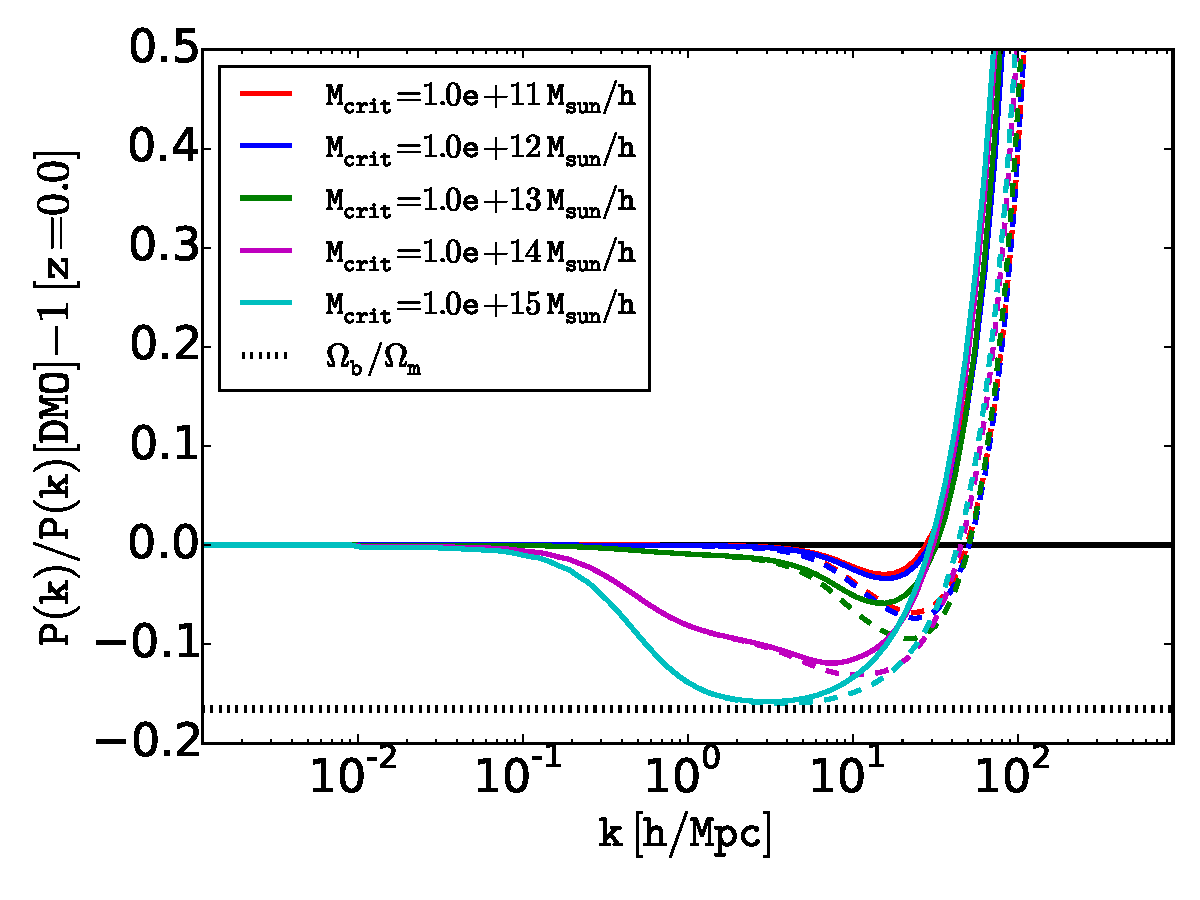
\includegraphics[width=0.48\linewidth]{figures/p3-figures/pk_ratio_z0.0.pdf}
	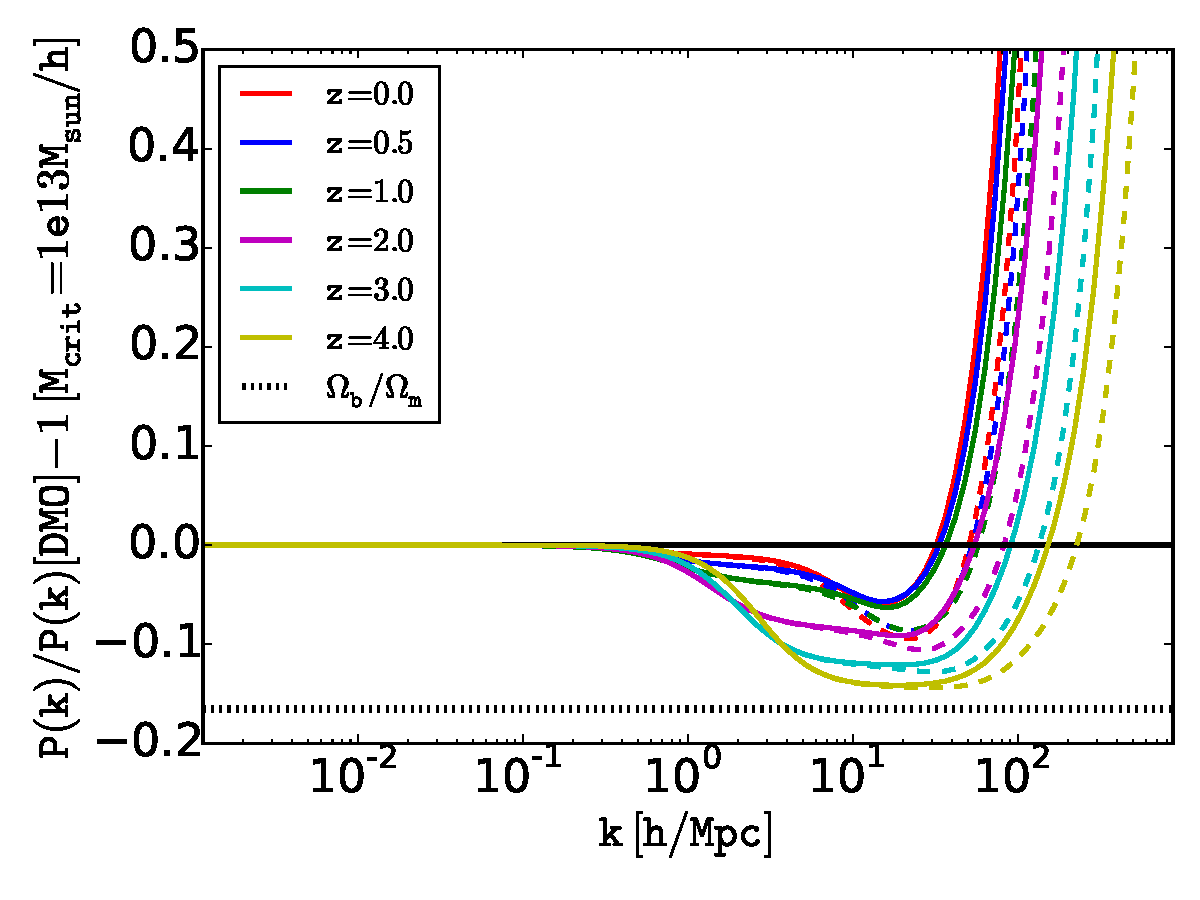
\includegraphics[width=0.48\linewidth]{figures/p3-figures/pk_ratio_Mcrit_1d13.pdf}
	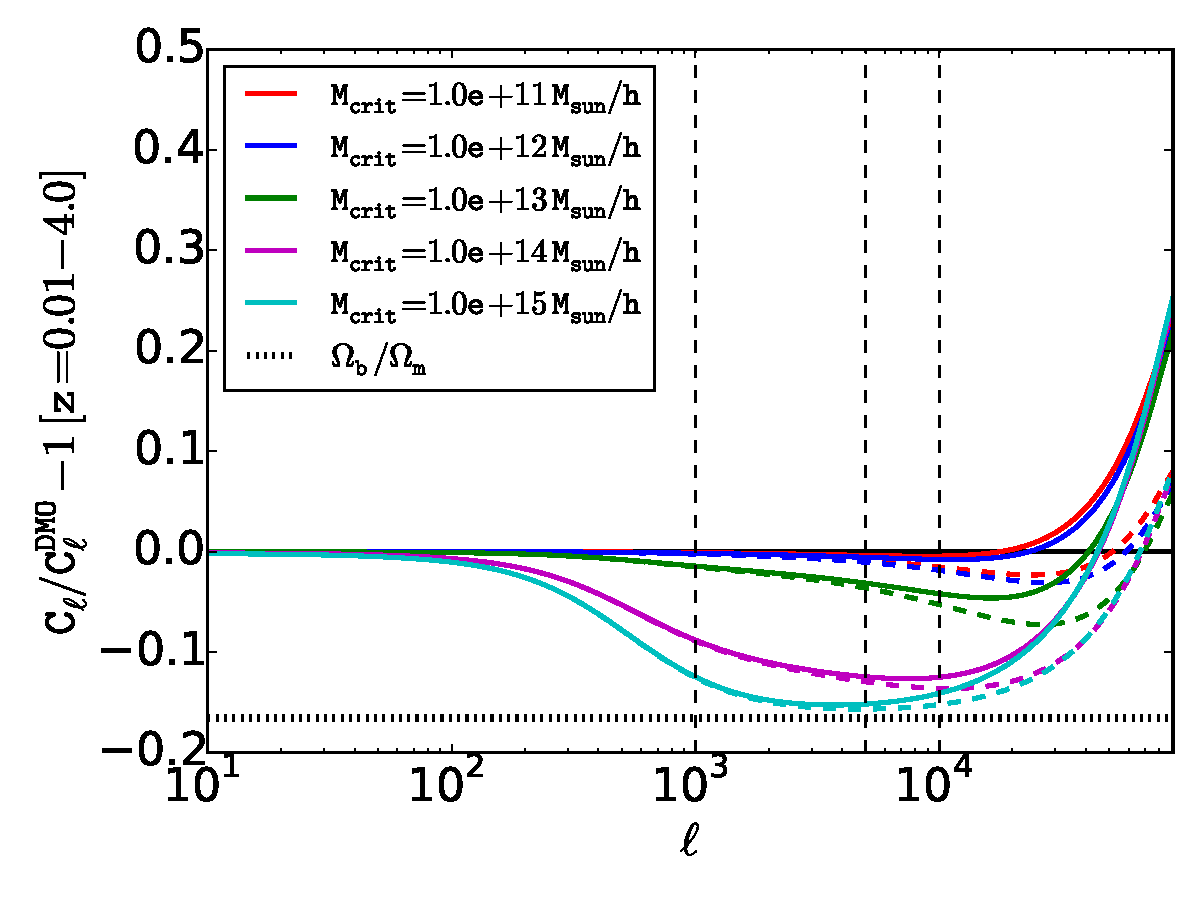
\includegraphics[width=0.48\linewidth]{figures/p3-figures/cl_ratio_nobin.pdf}
	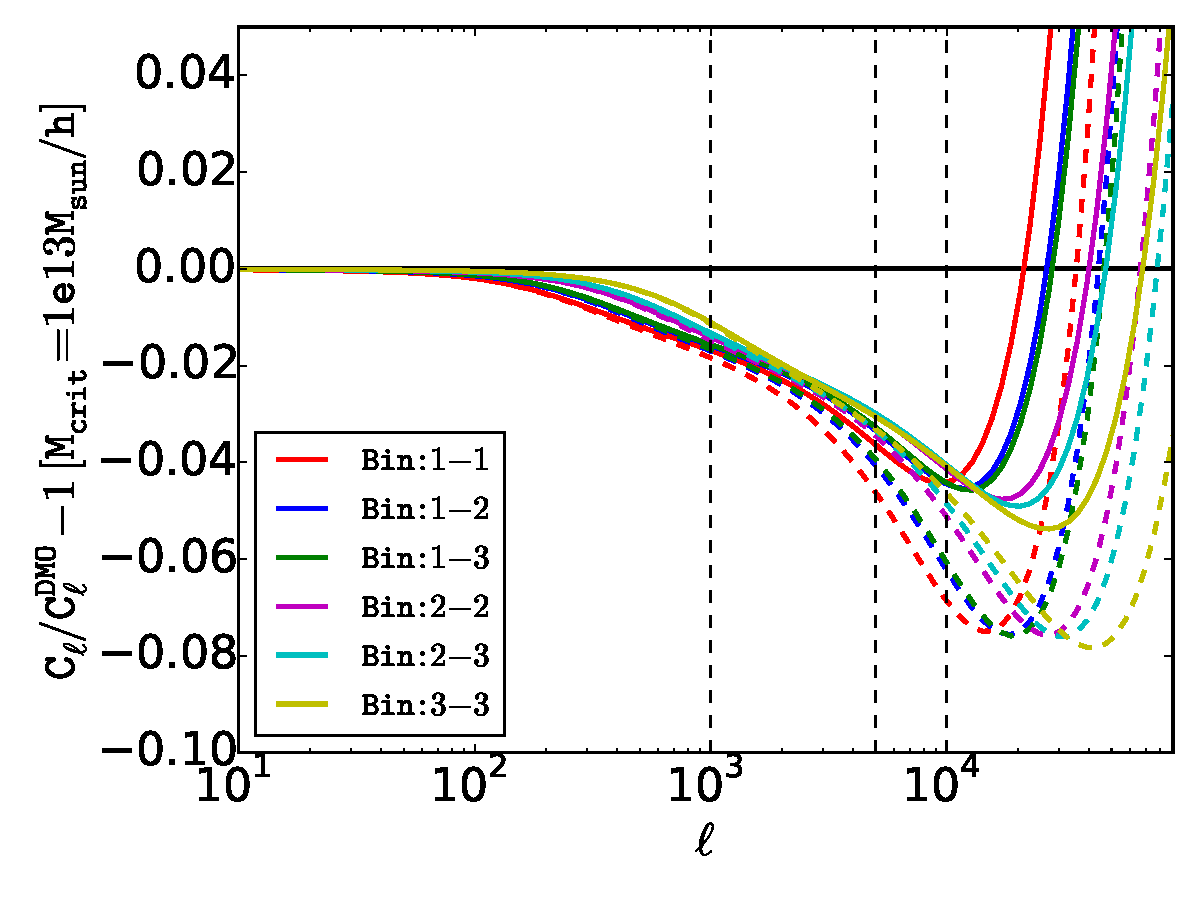
\includegraphics[width=0.48\linewidth]{figures/p3-figures/cl_ratio_bins_Mcrit_1e13.pdf}

	\caption{Top row: Relative deviation of the matter power spectrum predicted by the BAR model from the DMO model predictions as a function of $k$ for different $M_{\rm crit}$ at redshift zero (left) and for fixed $M_{\rm crit} = 10^{13} h^{-1} M_{\bigodot}$ and different redshifts (right). Bottom row: Relative deviation of the shear power spectrum ($C_{\ell}$) predicted by the BAR model from DMO model predictions for different $M_{\rm crit}$ in one big redshift bin (left) and for three tomographic redshift bins and fixed $M_{\rm crit} = 10^{13} h^{-1} M_{\bigodot}$ (right). Dashed lines are the calculations without adiabatic contraction (AC) and solid lines with adiabatic contraction (AC). The horizontal dashed line shows the cosmic baryon fraction.}
	\label{p3:fig:pkandcl}
\end{figure}
\clearpage

In this section we try to draw a comparison between the baryonic model (BAR) and the dark-matter only (DMO) model. We would like to establish an understanding of the scales where the baryonic corrections become important and how these scales changes with redshift and the only free parameter, $M_{\rm crit}$.

Figure \ref{p3:fig:pkandcl} (top-left panel) shows the relative differences between the BAR and DMO predictions for the matter power spectrum, also referred as {\it boost} in this article. There is only one free parameter of the baryonic model, $M_{\rm crit}$ which regulates the amount of AGN feedback and which is introduced in section \ref{p3:sec:icm}. The overall shape of the deviation is similar in all cases for various $M_{\rm crit}$ and redshifts: the BAR model follows the DMO model for large scales, suffers a deficit in power at intermediate scales due to flatter gas profile compared to the NFW profile and finally the power shoots up due to the central stellar component. Also without adiabatic contraction (AC) the raise in the matter power spectrum occurs at very small scales, but including AC effect this raise can be seen at comparatively lower $k$ or larger scales. This is because AC makes the profile steeper in the centre and shallower in the outskirts.

At redshift 0 (top-left panel of figure \ref{p3:fig:pkandcl}), the baryonic correction starts showing up (more than 1\%) at $k \sim 5\  h/Mpc$ for models with negligible AGN feedback (lower $M_{\rm crit}$), whereas for more extreme AGN feedback models (higher $M_{\rm crit}$) this correction is important at much larger scales like $k \sim 0.1\  h/Mpc$. In our fiducial BAR model with $M_{\rm crit} = 10^{13} h^{-1} M_{\bigodot}$, the baryonic effects become significant, i.e., more than 1 percent, at $k \sim 0.5\  h/Mpc$. The maximum dip in the intermediate scales vary for different $M_{\rm crit}$; for the most extreme models where AGN feedback can push all the gas out of the halo, this dip is nearly the cosmic baryon fraction, $\Omega_b/\Omega_m$. However, for more a realistic model ($M_{\rm crit} = 10^{13} h^{-1} M_{\bigodot}$) this dip is nearly 7-8\%. For more optimistic models like $M_{\rm crit} = 10^{12} h^{-1} M_{\bigodot}$, this dip is even smaller, nearly 4-5\%. Therefore, we can conclude the more extreme AGN feedback models triggers the deviation of matter power spectrum from DMO model at larger scales and also the dip in the power at intermediate scales can be as large as the cosmic baryon fraction in case where all the gas are pulled out by the AGN feedback, however, for more realistic and optimistic models, the deviation starts at relatively small scales and also the maximum dip is comparatively smaller.

Figure \ref{p3:fig:pkandcl} (top-right panel) shows the same quantity for a fixed $M_{\rm crit} = 10^{13} h^{-1} M_{\bigodot}$ at different redshifts. If we go to higher redshift, the overall shape of the deviation of the BAR matter power spectrum from the prediction of the DMO model (boost) is nearly the same as at redshift zero, however, the scales and the maximum dip amplitude at various redshifts change. We see that at higher redshifts, the dip starts to trigger at larger scales and also the maximum dip converge to the cosmic baryon fraction.

In figure \ref{p3:fig:pkandcl} (bottom-left panel), the baryonic correction to $C_{\ell}$ is shown in one big redshift bin ($z=0.01-4.0$). Here, the shear power spectrum starts to deviate from DMO predictions at about $\ell =100$ for the most extreme AGN feedback models and at $\ell$ of about several thousands for models with weak AGN feedback. For our realistic model (green curve), this deviation occurs at about $\ell \sim 700$. The maximum dip in power is very similar to that of the matter power spectrum explained above. It is worth noticing that for $\ell=10000$ the deviation is very significant for the realistic model ($M_{\rm crit} = 10^{13} h^{-1} M_{\bigodot}$), however, it is negligible for the optimistic model ($M_{\rm crit} = 10^{12} h^{-1} M_{\bigodot}$). Because these are the cases that we study in our likelihood analysis, we will show in section \ref{p3:sec:cosmology} that this behaviour is consistent with the cosmological parameter estimation with these models.


%===============================================================================



%===============================================================================
\section{Fiducial model and mock datasets}
\label{p3:sec:fiducial}

In this section, we would like to mention two factors that are quite important for our experiments - fiducial parameters and mock datasets.  The fiducial parameters assumed in this work, particularly about cosmology, baryonic model and Euclid mission, are very standard. Also the mock datasets generated are correctly contaminated with random noise. Following are the key numbers and information about the fiducial model assumed and mock datasets:

\begin{enumerate}

\item We used WMAP - 5th year cosmology  as our fiducial model with
$[\Omega_m,\allowbreak \Omega_b,\allowbreak h,\allowbreak n_s,\allowbreak
\sigma_8,\allowbreak w_0,\allowbreak w_a]$ as
$[0.279,\allowbreak 0.0462,\allowbreak 0.701,\allowbreak 0.96,\allowbreak
0.817,\allowbreak -1.0,\allowbreak 0.0]$. We assume the equation of state of dark-energy is redshift dependent as \citep{2001IJMPD..10..213C,2003PhRvL..90i1301L},
\begin{equation}
	w(a) = w_0 + (1-a)w_a
\end{equation}

where, $a = 1/(1+z)$ is the scale factor at redshift $z$.

\item We used three redshift bins to do the tomographic analysis with boundaries $[0.01, 0.8, 1.5, 4.0]$. So we calculated a total of six spectra - three auto-spectra between bins 1-1, 2-2 and 3-3 and three cross-spectra between bins 1-2, 1-3 and 2-3. 

\item We perform the likelihood analysis for different $\ell_{max}$ with $\ell_{min}=10$ and 100 equally spaced logarithmic bins. So the bin sizes for the likelihood analysis with different $\ell_{max}$ are different.

\item We assumed that the mean redshift of the source distribution to be nearly 1.0 which gives approximately 50 galaxies per arc min$^2$ and $f_{\rm sky}=0.55$ which resembles Euclid like survey.

\item For the baryonic model, we used the realistic AGN feedback model $M_{\rm crit}= 10^{13} h^{-1}M_{\bigodot}$ as the fiducial value for total nine $\ell_{max}$ (1000, 2000, 3000, 4000, 5000, 6000, 8000, 10000, 20000). We also performed one case with more optimistic model $M_{\rm crit} = 10^{12} h^{-1}M_{\bigodot}$ for $\ell_{max}=10000$. So there are ten cases in total. 

\item We used our fiducial model stated above to generate shear power spectrum $C_{\ell}$ for these ten cases and perturbed all $C_{\ell}$ with normally distributed multi-variate random numbers drawn from a distribution with mean $C_{\ell}$ and the corresponding covariance matrix. These $C_{\ell}$ are catalogued and constitute the mock data sets. So, there are total ten mock data sets. In figure \ref{p3:fig:bestfit} we show the mock datasets up to $\ell_{max}=20000$ for the six spectra and the best fits (which will be discussed in section \ref{p3:subsec:goodness}).

\end{enumerate}


\begin{figure}[p]
\centering
  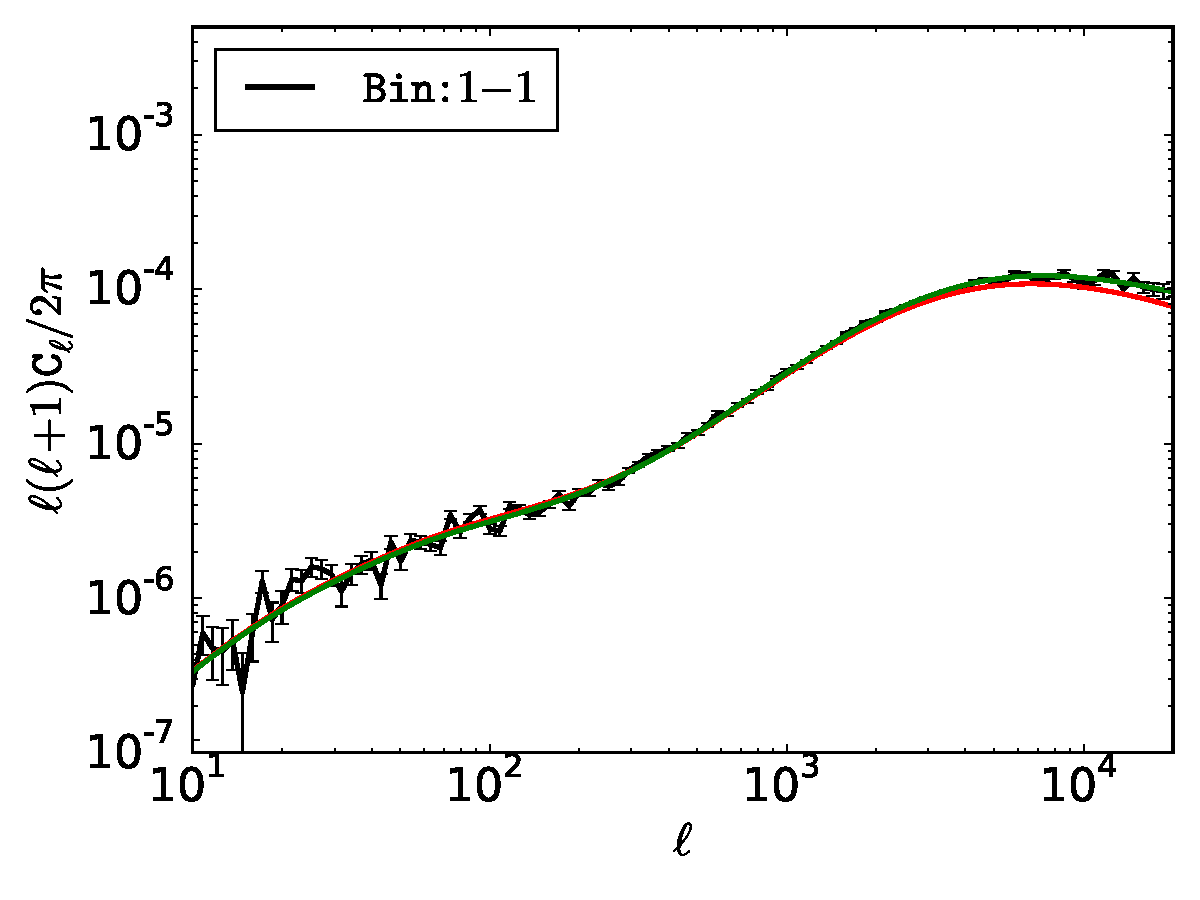
\includegraphics[width=0.48\linewidth]{figures/p3-figures/bestfit_1-1.pdf}
  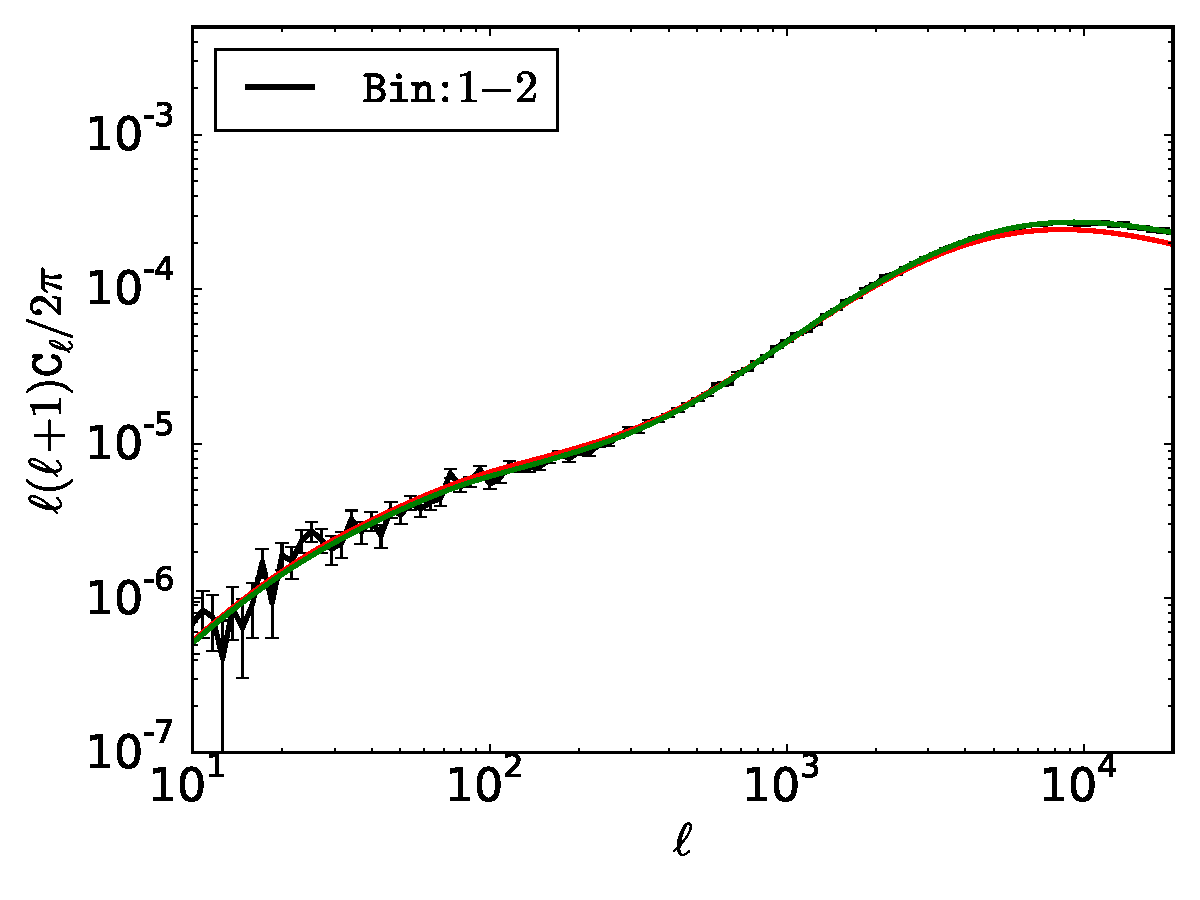
\includegraphics[width=0.48\linewidth]{figures/p3-figures/bestfit_1-2.pdf}
  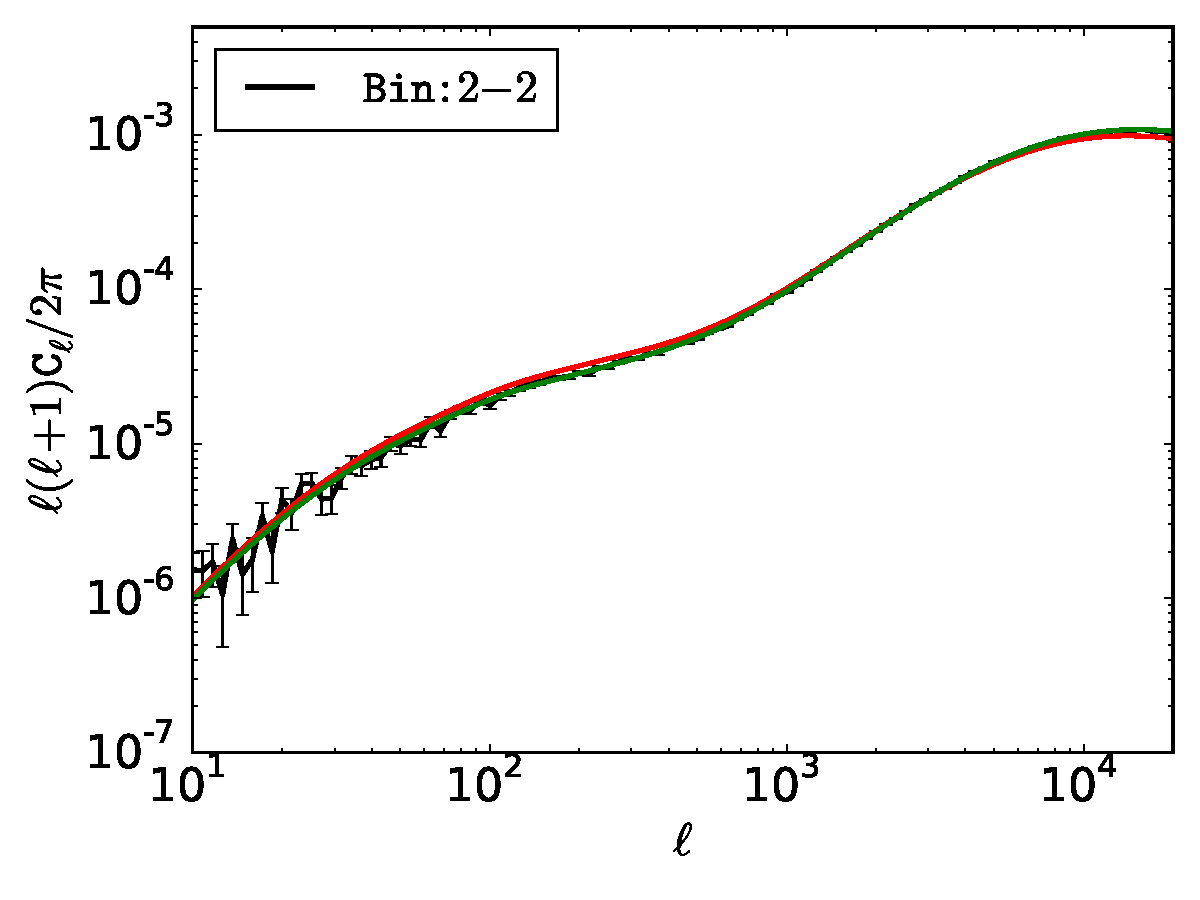
\includegraphics[width=0.48\linewidth]{figures/p3-figures/bestfit_2-2.pdf}
  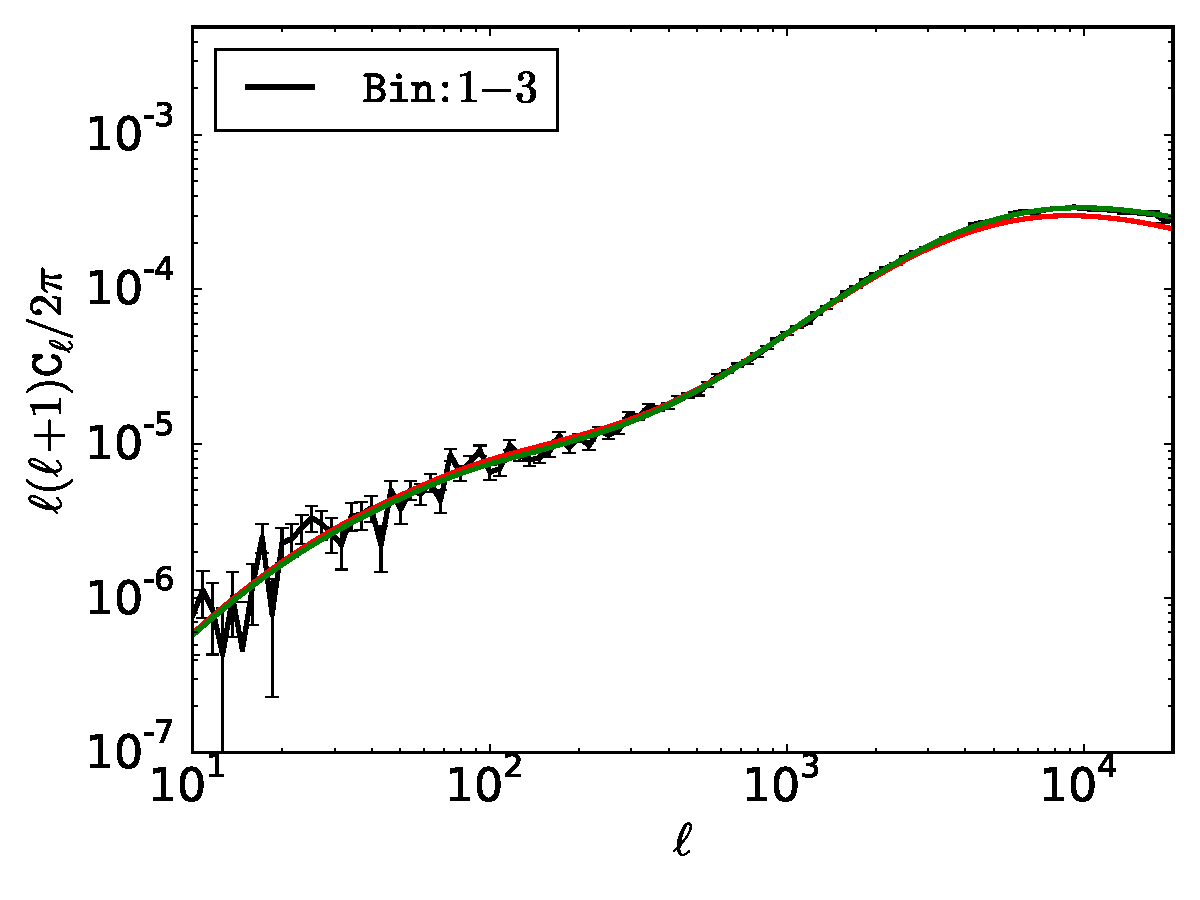
\includegraphics[width=0.48\linewidth]{figures/p3-figures/bestfit_1-3.pdf}
  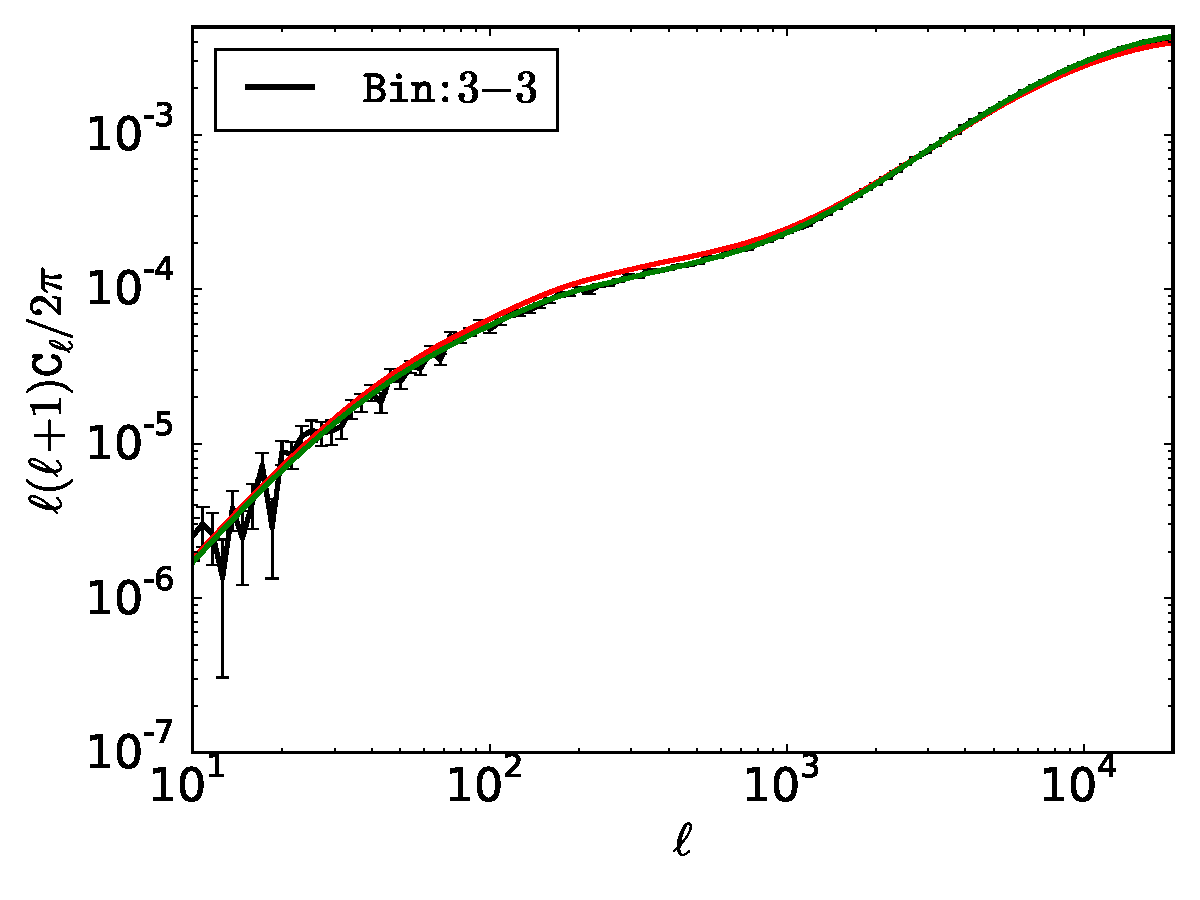
\includegraphics[width=0.48\linewidth]{figures/p3-figures/bestfit_3-3.pdf}
  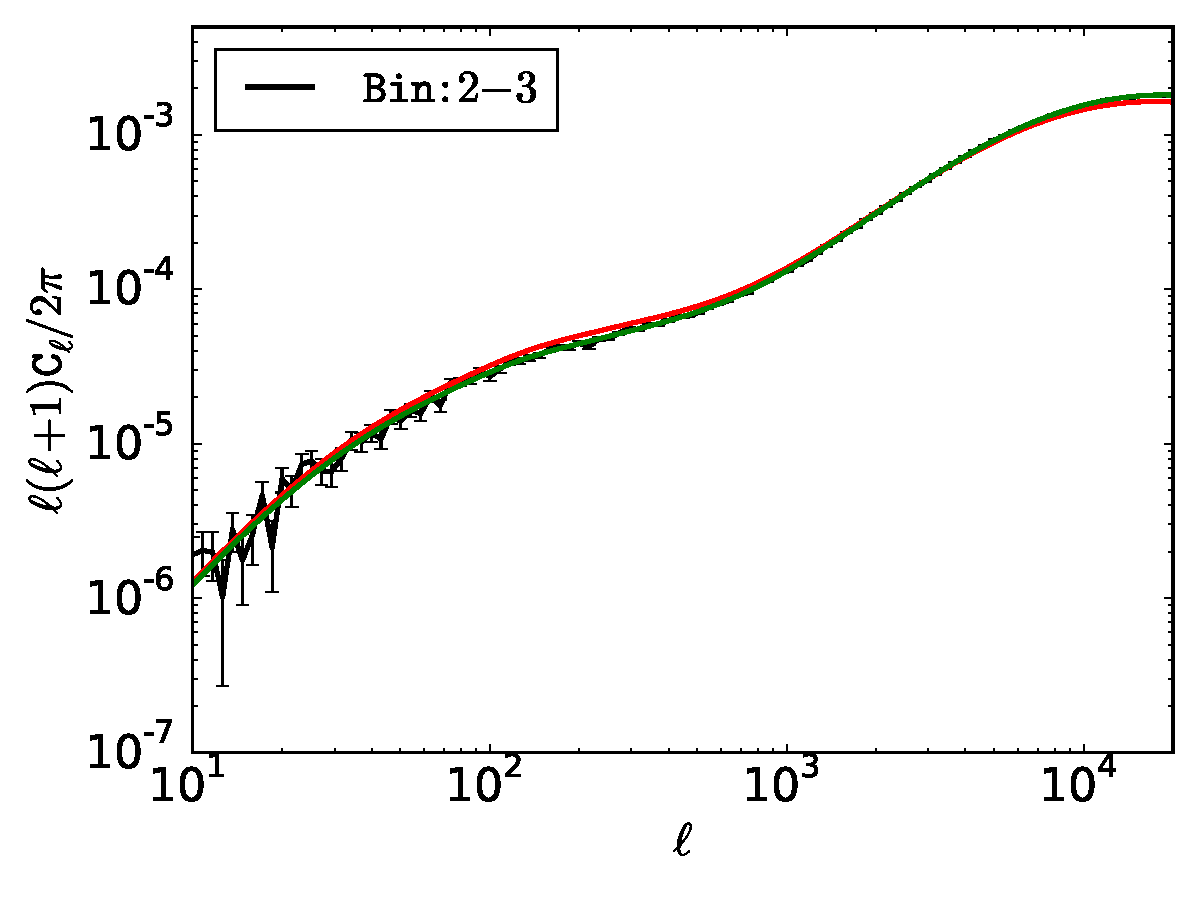
\includegraphics[width=0.48\linewidth]{figures/p3-figures/bestfit_2-3.pdf}

  \caption{Mock datasets (including random noise) for $\ell_{max}=20000$ in all six spectra (in black). The left column shows the three auto-spectra and the right column shows the three cross-spectra. Solid lines show the best fit for the DMO (red) and BAR (green) models.}
  \label{p3:fig:bestfit}
\end{figure}
\clearpage

For each bin combination (1-1,1-2 etc), the length of the data vector ($\ell$ or $C_{\ell}$) is 100. Therefore, the total number of data points in each data set is 600. However, the two cross-spectra, 1-2 and 1-3, are highly correlated which actually leads us to have only 5 degree of freedom for each $\ell$. Therefore, the total number of degree of freedom in each data set is about 492 (500 - 8 free parameters). Hence, the best fit to each dataset can have a $\chi^2$ in the range 492 $\pm \sqrt{(2\times 492)}$ which is between 470 and 514.

In figure \ref{p3:fig:pkandcl} (bottom-right panel), we show the boost for the unperturbed (without random noise) mock datasets up to very high $\ell_{max}$ with the corresponding DMO model. In all six curves of this figure, we kept $M_{\rm crit}=10^{13} M_{\bigodot}$. The auto-spectra in the first bin (1,1), starts deviating (more than 1\%) from the DMO model at about $\ell=300$ whereas the auto-spectra of the third bin (3,3) starts showing deviation at nearly $\ell=800$. All other auto-spectra and cross-spectra are between these two extremes. This behaviour is justified by looking at the same figure in upper-right panel, which shows the redshift evolution of the correction for the same $M_{\rm crit}$. It can be seen that at higher redshifts, the BAR matter power spectrum starts to deviate from DMO at smaller scales but also induces a larger dip at intermediate scales due to gas expulsion. This behaviour can be seen in the bottom-right panel. The $C_{\ell}$ in the lower redshift bin (1-1) starts deviating from DMO at larger scales as compared to the higher redshift bin (3-3), but the maximum dip in the two cases can be seen in the higher redshift bin (3-3). If we compare this to the bottom-left panel of the same figure, one can notice that the baryonic correction becomes even important when binning in redshift rather than using one big redshift bin. This provides additional constraints on $M_{\rm crit}$ while performing the analysis in tomographic bins compared to poorer constraints when only one bin is used.


%===============================================================================
\begin{figure}[p]
\centering
\centering

  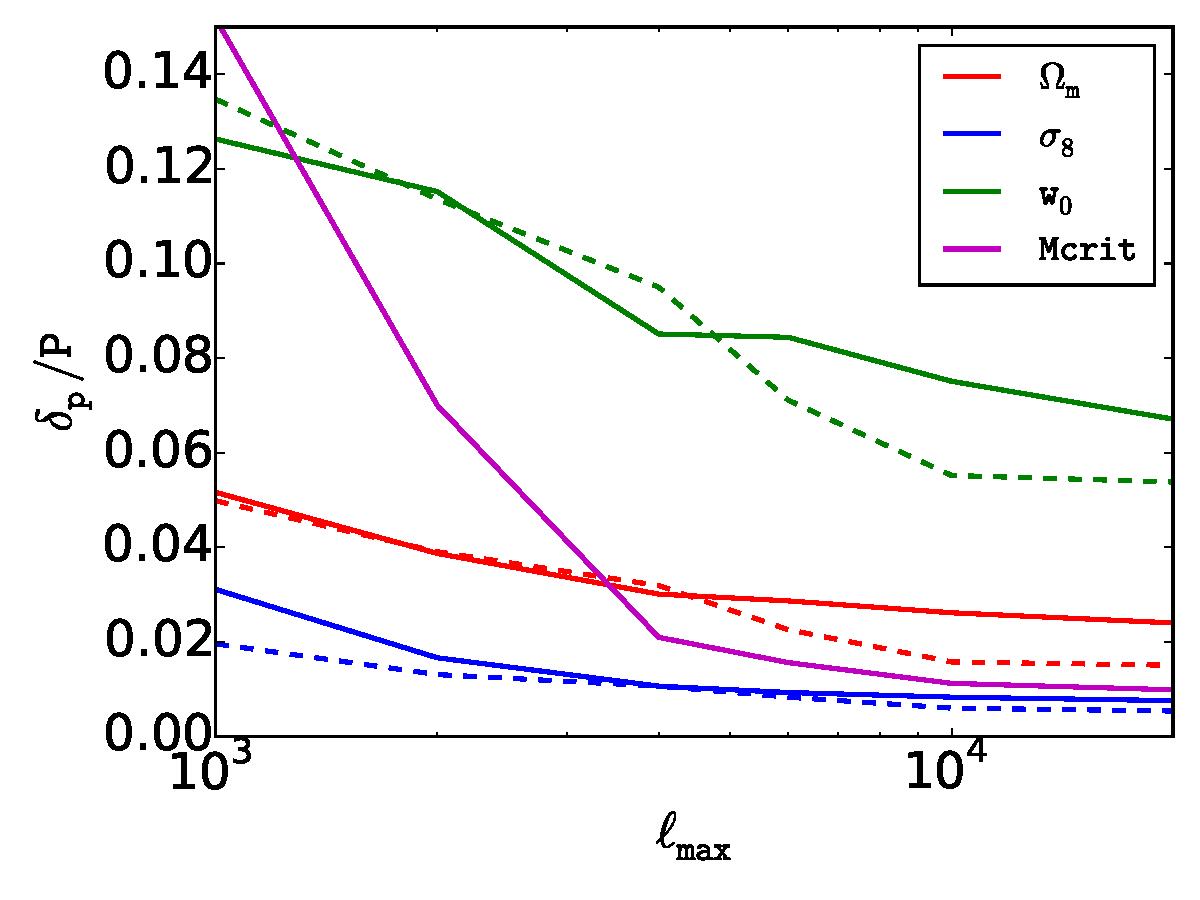
\includegraphics[width=0.8\linewidth]{figures/p3-figures/errors_euclid.pdf}
  \caption{Relative 1$\sigma$ errors on different cosmological parameters as a function of $\ell_{max}$ for $M_{\rm crit}=10^{13} h^{-1} M_{\bigodot}$. Solid lines are for the BAR model and dashed curves are for the DMO model. Horizontal black dashed lines mark the $\pm 1$ and vertical black dashed lines shows important scales.}
  \label{p3:fig:errors}
\end{figure}
\clearpage


\section{Likelihood analysis and cosmological implications}
\label{p3:sec:cosmology}

We performed a likelihood analysis using MCMC to explore the cosmological parameter space for nine different $\ell_{max}$ (1000, 2000, 3000, 4000, 5000, 6000, 8000, 10000, 20000) using $M_{\rm crit}=10^{13} h^{-1} M_{\bigodot}$, which is our most realistic model, and for $\ell_{max}=10000$ using $M_{\rm crit}=10^{12} h^{-1} M_{\bigodot}$ which is our optimistic model. 

We run MCMC on the ten mock datasets obtained adopting both the DMO and BAR models, therefore we run a total of 20 MCMC. Each MCMC is performed using the publicly available code COSMOMC \citep{2002PhRvD..66j3511L}, with 16 chains in each case. So total 320 CPUs are used for nearly 10 days to reach the desired convergence. The whole analysis required about 76800 hours.

We demonstrate the results of the MCMC and the interpretation in the following two sections, targeting particularly the precision and accuracy in predicting the cosmological parameters. 

\begin{figure}[p]
\centering
\centering
  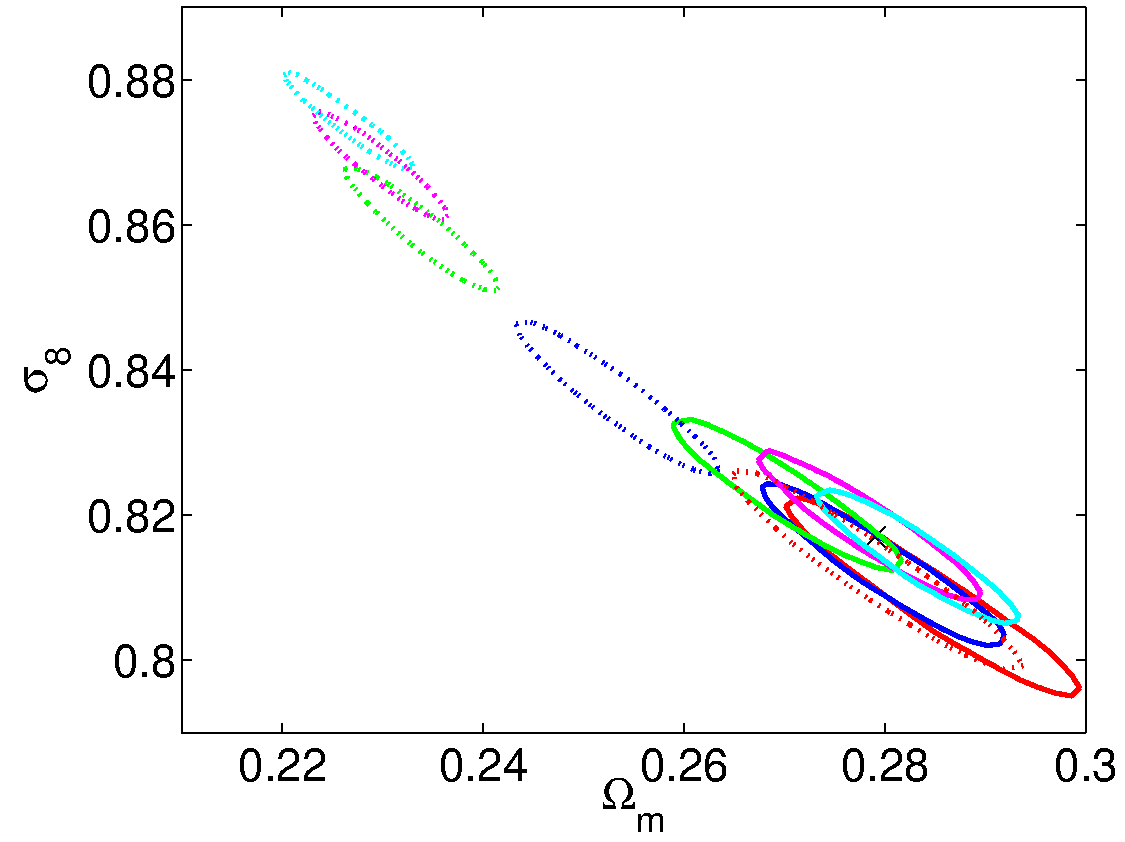
\includegraphics[width=0.48\linewidth]{figures/p3-figures/Om_s8.pdf}
  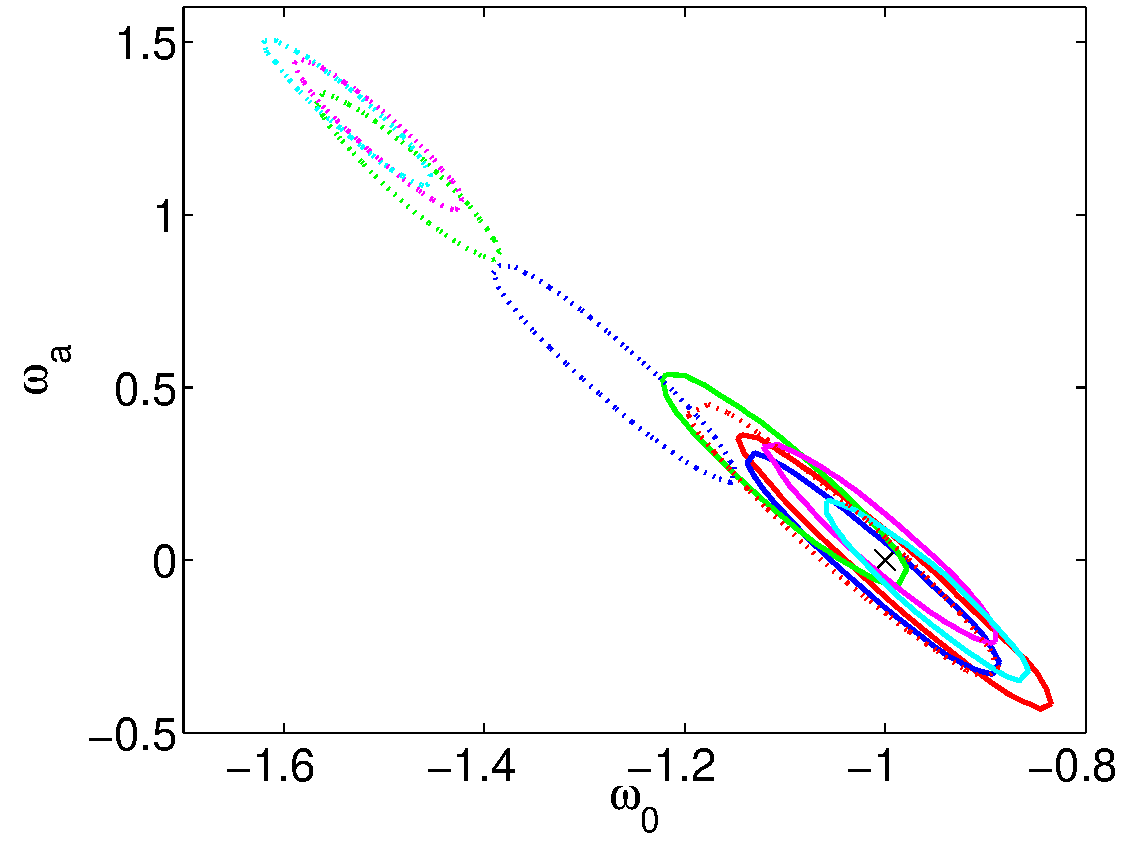
\includegraphics[width=0.48\linewidth]{figures/p3-figures/w0_wa.pdf}
  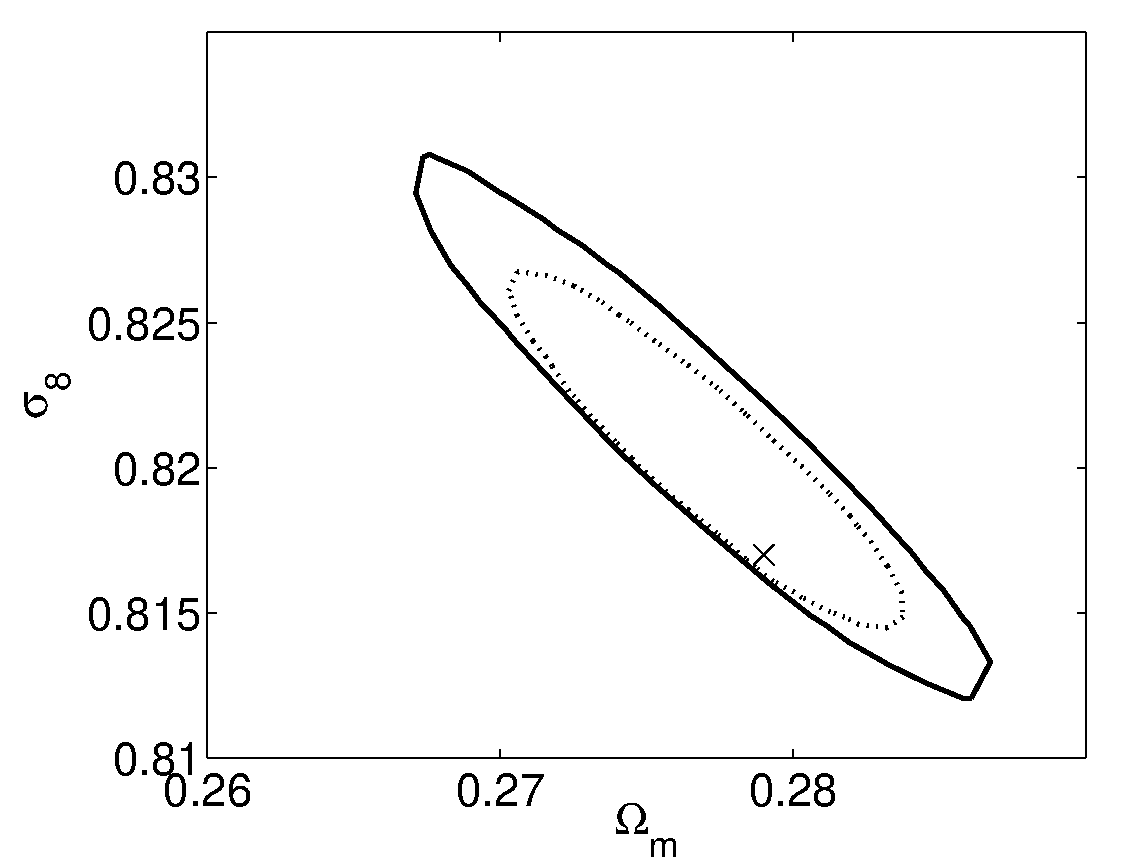
\includegraphics[width=0.48\linewidth]{figures/p3-figures/Om_s8_1d12.pdf}
  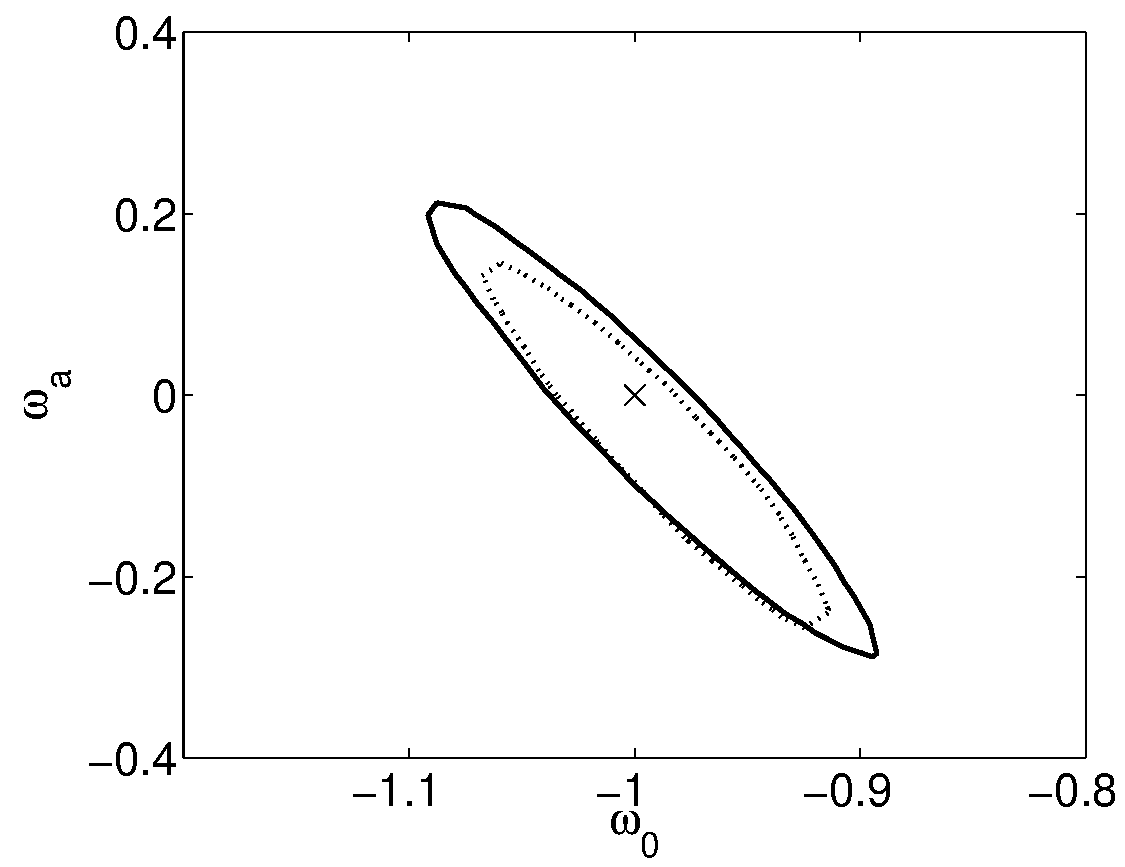
\includegraphics[width=0.48\linewidth]{figures/p3-figures/w0_wa_1d12.pdf}

  \caption{Top row: 1$\sigma$ 2D error ellipses for different cosmological parameters using mock datasets with $M_{\rm crit}=10^{13} h^{-1} M_{\bigodot}$ and different $\ell_{max}=$ 3000 (red), 5000 (blue), 8000 (green), 10000 (magenta), 20000 (cyan). Bottom row: 1$\sigma$ 2D error ellipses using mock datasets with $M_{\rm crit}=10^{12} h^{-1} M_{\bigodot}$ for $\ell_{max}=$ 10000. All solid curves are for the BAR model and dashed curves are for the DMO model.}
  \label{p3:fig:mcmc}
\end{figure}
\clearpage

%---------------------------------------------------------------------------------------------


\subsection{Precision in cosmology}

Future experiments, like Euclid, are expected to provide very tight constraints on cosmological parameters. Here we show the constraints expected from using the weak lensing shear power spectrum as a function $\ell_{max}$. Figure \ref{p3:fig:errors} shows the relative variance of four cosmological parameters and one baryonic parameter using both models, BAR (solid curves) and DMO (dashed curves). The matter density of the Universe ($\Omega_m$) and the amplitude of fluctuations ($\sigma_8$) are the most constrained parameters, however, other parameters like the equation-of-state of dark-energy today ($w_0$) are relatively less constrained. The overall behaviour of all parameters is the same, weak constraints for small $\ell_{max}$, better constraints with increasing $\ell_{max}$ and a flattening beyond $\ell_{max}\sim 8000$. The constraints derived from the BAR model are relatively weaker than the constraints derived from DMO model, which is the consequence of the extra parameter, $M_{\rm crit}$. 

The normalized matter density of the Universe $\Omega_m$ can already be determined up to 5\% at $\ell_{max}$=1000 which improves as good as 2-3\% at $\ell_{max}$=8000 whereas the amplitude of fluctuations $\sigma_8$ can be determined much better at corresponding scales. At $\ell_{max}$=1000, $\sigma_8$ can be known up to 3\% and these constraints improves better than 1\% at $\ell_{max}$=8000. After $\ell_{max}$=8000, the variance of both the parameters remains the same and no further constraints can be drawn by going up to lower scales or higher $\ell_{max}$. There is a certain degeneracy in these two parameters which can be seen in figure \ref{p3:fig:mcmc} upper-left panel, where different colours represent different $\ell_{max}$.

The constraints on the two parameters describing the redshift evolution of the equation of state of dark energy, $w_0, w_a$ can also be improved with this kind of experiments. At $\ell_{max}$=1000 $w_0$ can only be determined as good as 12\%, whereas for $\ell_{max}$=8000 it can be constrained up to 6-7\% and with the same precision for higher $\ell_{max}$. However, the constraints on $w_a$ are much weaker. The absolute error on $w_0$ is nearly 0.35 for $\ell_{max}$=1000, $\sim$0.18 for $\ell_{max}$ = 8000 and the same afterwards. 

The flattening of the relative errors of the parameters indicates that there is no gain in precision of cosmological parameters estimation after a certain threshold $\ell_{max}\sim 8000$. In practice, an experiment like Euclid may provide us with very high quality data to even resolve and measure the shear power spectrum at $\ell_{max}$ as high as $10^5$, but our analysis shows that the constraints becomes constant after $\ell_{max}\sim 8000$ and no further improvement can be achieved.

This forecast suggests that by measuring $C_{\ell}$s up to $\ell_{max}\sim 8000$, one can constrain $\Omega_m$ to about 2\% precision and $\sigma_8$ to about 0.5\% precision without any loss of information from high $\ell$s and including baryonic physics. However, $w_0$ can only be constraints up to 6-7\% with some information about $w_a$, the time derivative of the equation of state of dark energy.

\begin{figure}[p]
\centering
\centering

  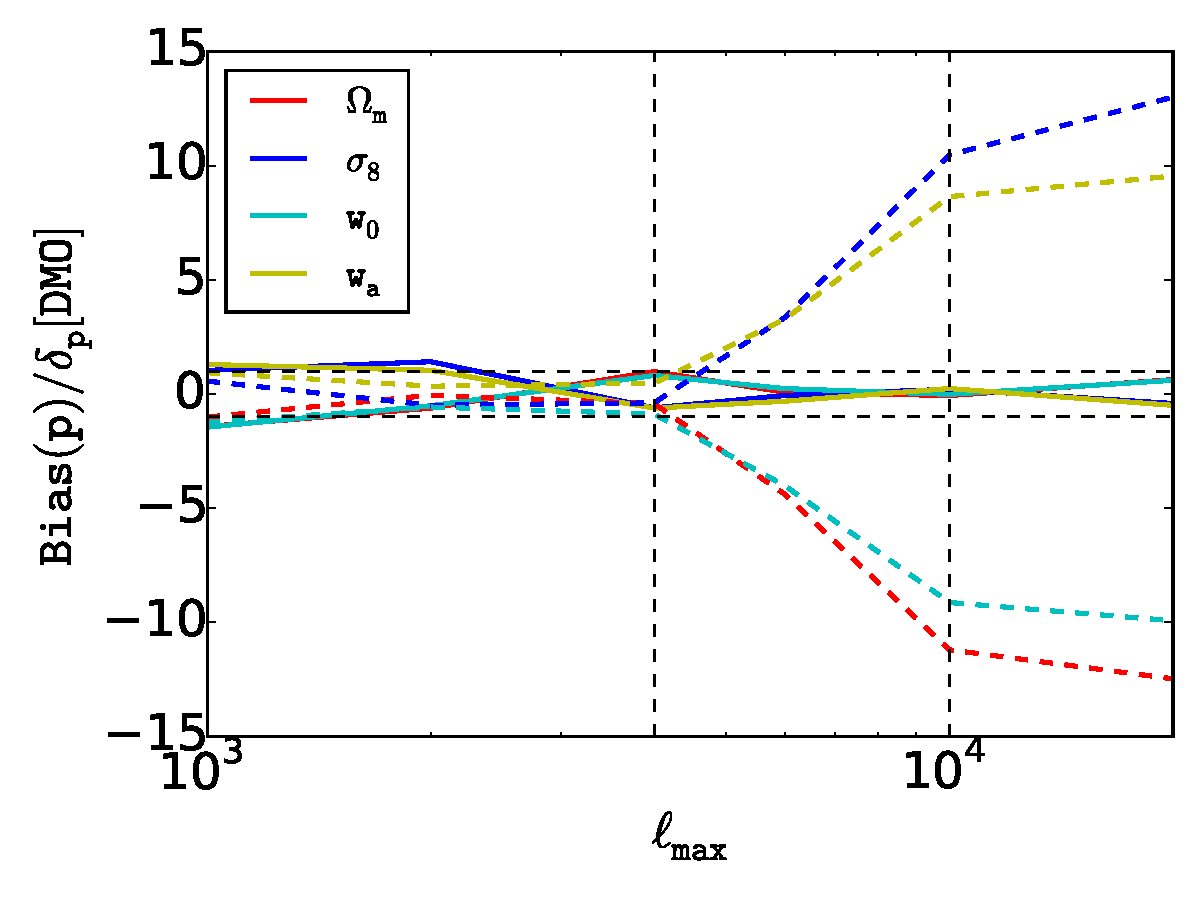
\includegraphics[width=0.8\linewidth]{figures/p3-figures/bias_lmax.pdf}
  \caption{The ratio of bias and 1$\sigma$ error of various cosmological parameters as a function of $\ell_{max}$ for $M_{\rm crit}=10^{13} h^{-1} M_{\bigodot}$. Solid lines are for the BAR model and dashed curves are for the DMO model. Horizontal black dashed lines mark the $\pm 1$ and vertical black dashed lines shows important scales.}
  \label{p3:fig:bias}
\end{figure}
\clearpage

%---------------------------------------------------------------------------------------------

\subsection{Accuracy in cosmology}

When precision cosmology is the goal, one should also take into account the ability to recover the cosmological parameter accurately. If there are systematic errors in the model, one can still derive very tight constraints from the wrong model, but the recovered parameters will be wrong or biased as compared to the true values. In this section we will present the results from our analysis of the bias in the cosmological parameters due to the lack of baryonic physics in DMO models and we will assess if these biases are significant. We define bias as the difference between the mean value of the parameter in MCMC and its fiducial or true value. 


Figure \ref{p3:fig:mcmc} shows the 1$\sigma$ error ellipses of cosmological parameters when the model is BAR (solid curves) and DMO (dashed curves). For small $\ell_{max}$, the two models are indistinguishable, a consequence of the fact that baryonic physics becomes more important only at smaller scales. But as we go higher and higher in $\ell_{max}$, the target density of the DMO model shifts further from the true target density, however, the BAR model remains at the correct location.  We find that for all BAR models this bias is smaller than the 1$\sigma$ error of the parameter, however, the bias in the parameters obtained fitting for the DMO model increases with increasing $\ell_{max}$.

Figure \ref{p3:fig:bias} shows the ratio of these biases and the 1$\sigma$ error on the cosmological parameters as a function of $\ell_{max}$ for the two models, BAR (solid curves) and DMO (dashed curves). The bias never exceeds the 1$\sigma$ error for the BAR models, however, it does for the DMO models only after $\ell_{max} \sim 4000$. This is again a consequence of the fact that baryonic physics is only important at smaller scales. This indicates that if we only perform our experiment up to $\ell_{max}$=4000, no baryonic physics needs to be taken into account, however, if one is interested in $\ell_{max}>4000$ baryonic physics becomes very important. After $\ell_{max}$=4000 the bias increases with $\ell_{max}$ and goes as big as 10$\sigma$ at $\ell_{max}$=10000 and remain flat after that. We see in the previous section that constraints on cosmological parameter can still be improved up to $\ell_{max}$=8000, but considering the wrong model, DMO, the cosmological parameters will be 5-10$\sigma$ away from the true values. So, in order to gain the best constraints on cosmology, baryonic physics must be taken into account. 



%---------------------------------------------------------------------------------------------

\subsection{An optimistic model}
We analysed the $\ell_{max}=10000$ case for our optimistic model with $M_{\rm crit}=10^{12} h^{-1} M_{\bigodot}$. As in our previous analysis, we performed two MCMC in this case too, fitting for the BAR model and for the DMO model. Figure \ref{p3:fig:mcmc} (bottom row) shows the 1$\sigma$ error ellipses of cosmological parameters. In this case the bias in the cosmological parameters does not exceed the $1\sigma$ error and hence is not a very troubling case. This was expected, as for lower $M_{\rm crit}$, baryonic physics is less important even at comparatively small scales as compared to cases where $M_{\rm crit}$ is higher. For example if we look at figure \ref{p3:fig:pkandcl} (bottom-left panel), we can see that for $M_{\rm crit}=10^{12} h^{-1} M_{\bigodot}$, the deviation of $C_{\ell}$ from the DMO model is negligible at $\ell=10000$. Hence, we actually expect smaller or no bias. 

%---------------------------------------------------------------------------------------------


%===============================================================================

\section{Discussion and conclusions}
\label{p3:sec:discussion}


In this work we first review the important theoretical framework necessary to calculate the matter power spectrum using the halo model and to compute the shear angular power spectrum in different redshift bins. We presented an analytic prescription to distribute baryons into two components -- the intra-cluster plasma in hydrostatic equilibrium within the halo, and the BCG, which dominates the mass distribution in the centre of the halo, and whose properties are well measured using abundance matching techniques. We also take into account the adiabatic contraction of the dark matter particles due to the central condensation of  baryons. We also compared these analytic density profiles to the simulations of \cite{2014MNRAS.440.2290M}, both dark-matter-only and baryonic with AGN feedback, and found a remarkable agreement. 

We model the shear power spectrum in the two models, BAR and DMO, and found that baryonic corrections are important after $k \sim 0.5\ h/Mpc$ in the matter power spectrum at redshift 0 for our most realistic AGN feedback model, which translates into $\ell \sim 800$ for the shear power spectrum in one big redshift bin. However, if binned in redshift space (lensing tomography), these corrections become larger in each bin and for each auto- and cross-correlation function. These baryonic corrections have one free parameter, $M_{\rm crit}$, which regulates AGN feedback, i.e., it controls how much gas will be inside the halo as a function of the halo mass. We believe the most realistic value of this parameter is near $10^{13} h^{-1}M_{\bigodot}$, which sets the most likely magnitude of  baryonic corrections.

We perform the likelihood analysis using MCMC for total ten different datasets. Nine of them assume our realistic model for the AGN feedback with $M_{\rm crit} = 10^{13} h^{-1}M_{\bigodot}$ but different $\ell_{max}$, and one assumes a less extreme (optimistic) model with $M_{\rm crit} = 10^{12} h^{-1}M_{\bigodot}$. For each mock dataset, we perform MCMC to fit for both models, BAR and DMO.

The main results of the likelihood analysis are summarized in figure \ref{p3:fig:mcmc}, \ref{p3:fig:errors} and \ref{p3:fig:bias}. The results are very interesting in two aspects: first, we found that the constraints on all cosmological parameters improve with increasing $\ell_{max}$, but after $\ell_{max} \sim 8000$, the variance of each parameter becomes nearly constant. This indicates that even if we go to higher $\ell_{max}$ (or smaller scales), no additional constraints on the cosmological parameters can be gained. Second, if the wrong model, in this case DMO, is fitted to the data, after $\ell_{max}=4000$ the mean recovered value of the parameters starts moving away from its true value. We refer to the difference between the true value and recovered mean value as bias in the cosmological parameter. The bias in the parameters becomes more than 1$\sigma$ after $\ell_{max}=5000$ and goes up to 10$\sigma$ for $\ell_{max}=10000$, remaining flat afterwards. So, there is a very interesting window from $\ell_{max}=4000-8000$ which is useful for improving the constraints on cosmology, but if wrong model like DMO is chosen, the recovered cosmology can be highly biased from few to 10-$\sigma$.

\subsection{Goodness of fit}


In the previous sections we see that for $\ell_{max}<4000$, there is no significant bias added to the determination of the cosmological parameters in our analysis, however, for $\ell_{max}>5000$ the bias exceeds 1$\sigma$ and keep increasing up to 10$\sigma$ with increasing $\ell_{max}$. The question here is: can we discard these biased models by looking at the goodness of fit? The answer to this question lies in figure \ref{p3:fig:chi2} where we show the ratio between the best fit $\chi^2$ in the DMO model and that in the BAR case as a function of $\ell_{max}$. This ratio is as little as 5-10\% up to $\ell_{max} \sim 5000$ but after that it only goes up to 25\% at $\ell_{max}=20000$ where bias is more than 10$\sigma$. Now, the reduced $\chi^2=1.25$ does not appear as such a bad fit for our cosmological measurements. So, by looking at the $\chi^2$ only, it is not really possible to discard a model. The same conclusion can be drawn from figure \ref{p3:fig:bestfit}, where we show the mock datasets of the six spectra (between different bins) for $\ell_{max}=20000$. In this figure, we also show the two best fit from the DMO model (in red) and the BAR model (green). As we expect, the green curve is a better fit to the data than the red curve. But if the green curve is not present in this figure, the red curve does not appear to be a very bad fit. So, when deriving constraints on cosmology from this kind of experiments, one should be extremely careful about the possible magnitude of baryonic effects at small scales, because, although the results obtained with the wrong model may appear as a good fit, the corresponding bias can be in fact as high as many $\sigma$. Also, the recovered parameters from the wrong model (DMO) move away from the true value with increasing $\ell_{max}$. This suggests a potential test for a given model, the cosmological parameter space should not move significantly when analysing up to different scales, the difference should only be seen in the variance of the parameters and not in its mean value.


\subsection{\texorpdfstring{$M_{\rm crit}$}{Mcrit} parameter}

The only free parameter in our BAR model, $M_{\rm crit}$, regulates the amount of gas inside the halo as a function of halo mass. We explore the consequences of what we believe to be a realistic model ($M_{\rm crit} = 10^{13} h^{-1}M_{\bigodot}$) in details considering nine different $\ell_{max}$. At $\ell_{max}=1000$, there is hardly any constraint drawn from weak lensing on this parameter, but as we increase $\ell_{max}$, baryonic physics become more and more important and thus constraints can be put on $M_{\rm crit}$. In fact, the constraints on this parameter increase rapidly from 15\% at $\ell_{max}=1000$ to 1-2\% at $\ell_{max}=4000$. After this, no significant improvement on the constraints can be gained on this parameter. The variance of $M_{\rm crit}$ becomes constant after nearly $\ell_{max}=8000$, which is what happens for the other cosmological parameters. So, with this kind of weak lensing experiment, $M_{\rm crit}$ (or $\log(M_{\rm crit})$) could be constrained up to 1-2\%, which is quite impressive.


\label{p3:subsec:goodness}
\begin{figure}[p]
\centering
  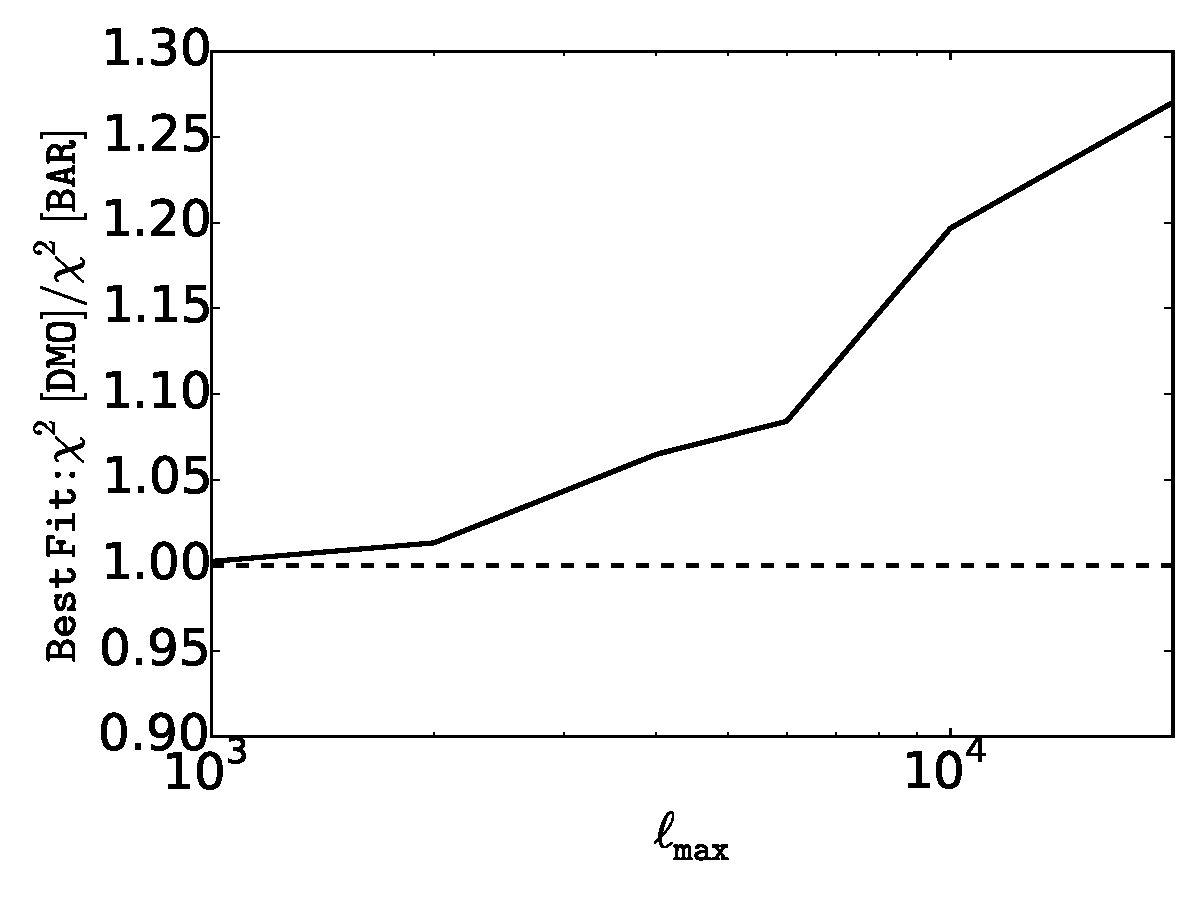
\includegraphics[width=0.48\linewidth]{figures/p3-figures/chi2.pdf}
  \caption{Showing the ratio of the best fit $\chi^2$ in DMO model and BAR model at different $\ell_{max}$.}
  \label{p3:fig:chi2}
\end{figure}
\clearpage


\subsection{Non-Gaussian covariance vs baryonic corrections}
\label{p3:sec:NG}
Being able to extract cosmological information from clustering data down to a few percent accuracy can be considered very optimistic. It can be jeopardized by many unresolved issues. The two most important issues are (i) baryonic physics at small scales, and (ii) non-Gaussian effects in the covariance matrix of the power spectrum. These two issues can be quantified in projected weak-lensing statistics, like the shear power spectrum. In this work, we primarily talk about the effect of baryonic physics at small scales on the shear power spectrum and its cosmological implications. However, we ignore the effect of non-Gaussianity (NG) on the covariance matrix. 

The NG contribution to the covariance becomes more important at small scales, like baryonic physics \citep{2009MNRAS.395.2065T, 2013PhRvD..87l3504T}. Now the question is, which one is more important to deal with and which one appears first when going towards smaller scales? This question does not have a very straightforward answer. Ignoring both  of these contributions may result in highly biased cosmological parameters estimations.

\cite{2012PhRvD..86h3504Y} (figure 9, right panel) shows the constraints on the amplitude of fluctuations ($\sigma_8$) as we go to smaller scales. If one considers only Gaussian errors, the constraints continue to improve until the instrumental shot noise kicks in. However, NG contribution are likely to dominate over Gaussian errors after $\ell=700$. But we cannot directly compare to this plots as the constraints depend on many other details. We can still compare the ratios of the NG and Gaussian contributions. At $\ell_{max}=10000$, the NG covariance is six times the Gaussian covariance. On the other hand, in figure \ref{p3:fig:bias} the bias in cosmology becomes close to 10$\sigma$ for $\sigma_8$ at $\ell=10000$. This means that the NG corrections are sub-dominant than the baryonic effects. However, our analogy is very hand-wavy and requires further study.

\subsection{The ideal configuration}

We explore the baryonic effects on the cosmological parameter estimation and found big bias in cosmological parameters if the analysis include $\ell>4000$. After this limit, the cosmological parameters start to become biased and mislead the constraints. However, the constraints keep improving up to $\ell=10000$. So the question arises, what is the ideal configuration to perform weak-lensing power spectrum analysis to put useful constraints on cosmology with Euclid-like surveys? 

We explore this answer in our analysis and stated our results in the previous sections. To summarize, the ideal configuration is to go as high as $\ell=8000$, including baryonic physics and marginalize over the baryonic parameters, in our case $M_{\rm crit}$. In this configuration, one can find unbiased estimates of the cosmological parameters. Having the unbiased estimates, we can also constrain the cosmological parameter space with much better accuracy than before. In this configuration, $\Omega_m$ and $\sigma_8$ can be estimated with nearly 2\% and 0.5\% respectively. The variance of the two parameters defining the redshift evolution of the equation of state of dark energy, $w_0$ and $w_a$ are 0.07 and 0.15 respectively. Along with cosmological parameters, the baryonic parameter $M_{\rm crit}$ can also be estimated to very high accuracy, as good as 1-2\%.

When dealing with real clustering datasets, we are also able to use independent constraints on the baryonic parameters, such as abundance matching data and/or X-ray data on individual halos, providing a solid understanding of the overall signal and the underlying baryonic effects.






%===============================================================================
\section{Acknowledgement}
I.M. would like to thank Prasenjit Saha, Uros Seljak and Ravi Sheth for useful discussions about the topic and their suggestions.
%==============================================================================
% Chapter 5: Paper 4
%==============================================================================

\chapter{Lensing Time Delays as a Substructure Constraint}
\label{p4:chap:time-delay-substructure}

\section{Introduction to the Paper}

Strong gravitational lensing (SL) is a very powerful tool to reconstruct the mass distribution
of the lens given the positions of the multiple images of the background source(s). 
Another observable
of the SL phenomenon is the time delay between two images of the same source,
due to the fact that two light rays from the same source, emitted at the
same time, travel different paths (and so the distances), and reach the same observer. 
If the source is variable, like a quasar or a supernovae etc., 
it is possible to measure these time delays. 

As described by equation \ref{eqn:timedelay}, 
the total time delay between two images 
is proportional to the comoving distance from the observer to the lens, 
and therefore depends
on the Hubble constant $H_0$. If the mass distribution of the lens
is known, it is possible to infer the $H_0$ by measuring the time delays.
However, this exercise is very sensitive to the mass distribution of the 
lens. Therefore, a very good understanding of the gravitational potential
of the lens is needed in order to measure the $H_0$ using the time delays.
This has been done by many authors in the past, where they derived necessary
constraints on $H_0$.

In this paper, we quantified the additional constraints provided by the time delays
on the mass distribution of the lens assuming a cosmological model (or $H_0$). 
We performed a principle component analysis (PCA)
using two types of mass maps of the lensing cluster SDSS J1004+4112 - one 
reconstructed with time delays data (TD) and other without it (NTD). The main
science driver of this paper is to identify and isolate those 
uncertainty modes that are present in NTD maps and are not in TD maps.
By successfully identifying these modes, we concluded that in the lensing clusters
where the steepness degeneracy is already broken by multiple background sources
at different redshifts, time delay information can be used to constrain
the lopsidedness of the cluster core.

\paragraph{Role:} Under the supervision of Dr. Prasenjit Saha, I started this project
by accumulating lensing data for SDSS J1004 cluster. Along with the multiple
images of three background sources, two time delays were also available for one 
of the background sources, which is a quasar. Employing this dataset, I reconstructed
30 mass maps using lensed images only, and 30 using lensed images plus two time
delays. I also computed the average mass map with optimal resolution in both
cases. The next step was to isolate the uncertainty modes that were present
in NTD maps, and not in TD maps. Each mass map is a grid of pixels, and for each
case total 30 maps were available. 
I computed the uncertainty/moment matrix for NTD models.
I isolated its principle component, which was the eigen-vector corresponding
to the largest eigen-value, that resembles the largest uncertainty
mode present in NTD models, and compared its effect to the reference 
mass model that we chose to be the average TD mass map. 

This paper has been published in {\it Publication of Astronomical Society of Japan} (PASJ). 
\\
Arxiv: \url{http://arxiv.org/abs/1412.3464}

\begin{publishedpaper}
  {\fontsize{18}{22}\selectfont\scshape
   Lensing Time Delays as a Substructure Constraint:\par
   A Case Study with the Cluster SDSS~J1004+4112\par}

  \vspace{1.25em}

  {\large
   Irshad Mohammed, Prasenjit Saha, and Jori Liesenborgs\par}

  \vspace{1.25em}
  {\small
   Published in \textit{Publications of the Astronomical Society of Japan}\par
   \url{https://arxiv.org/abs/1412.3464}\par}
\end{publishedpaper}

\begin{paperabstract}
Gravitational lensing time delays are well known to depend on
cosmological parameters, but they also depend on the details of the
mass distribution of the lens.  It is usual to model the mass
distribution and use time-delay observations to infer cosmological
parameters, but it is naturally also possible to take the cosmological
parameters as given and use time delays as constraints on the mass
distribution.  This paper develops a method to isolate what exactly
those constraints are, using a principal-components analysis of
ensembles of free-form mass models. We find that time delays
provide tighter constraints on the distribution of matter in 
the very high dense regions of the lensing
clusters.   We apply it to the cluster lens
SDSS J1004+4112, whose rich lensing data includes two time delays.  We
find, assuming a concordance cosmology, that the time delays constrain
the central region of the cluster to be rounder and less lopsided than
would be allowed by lensed images alone. This detailed information
about the distribution of the matter is very useful for
studying the dense regions of the galaxy clusters which are very
difficult to study with direct measurements.  A further time-delay
measurement, which is expected, will make this system even more
interesting.
\end{paperabstract}

\vspace{1em}
\noindent\textbf{Keywords:}
Gravitational lensing: strong,
galaxies: clusters: individual (SDSS J1004+4112).
\par
\vspace{1em}

\section{Introduction}

While $\Lambda$CDM cosmology is a very successful framework, the
underlying nature of both $\Lambda$ (dark energy) and CDM (dark
matter) remains unknown.  The interaction of baryons with both of
these is well understood during the linear-growth era of structures,
but less so when clusters and galaxies start to form.  $N$-body
simulations of CDM give dark-matter distributions which roughly
follows cuspy profiles with a characteristic radius, so-called
well-known NFW profiles \citep{1997ApJ...490..493N}, however
hydrodynamical simulations and other analytic studies show that in
the presence of baryons, NFW is no longer a good fit in the innermost
part of the haloes (see for example \cite{2014arXiv1409.8617S,2014arXiv1410.6826M}).
The distribution of matter in the innermost part of the galaxy
clusters is dominated by the baryonic component, particularly with BCG
and other elliptical galaxies. So, the distribution is different than
that of dark-matter and does not follow NFW profile, which is a very
good fit in the outskirts of the cluster. Due to the high potential
well of galaxies, some dark-matter contracts adiabatically making its
profile steeper at the centre \citep{1986ApJ...301...27B,2004ApJ...616...16G,
2005MNRAS.356..107R}. Generally, the centres of 
the BCG host active nuclei (AGN), which through feedback pushes 
the gas near the centre of the halo to the outskirts 
\citep{2005MNRAS.360..892D,2006Natur.442..539M, 
2013MNRAS.429.3068T, 2013MNRAS.432.1947M}.  For low mass halos 
AGN feedback can push all the gas outside the halo
whereas for high mass halos AGN feedback is not that strong. At the
very transition from big groups and galaxy clusters, the AGN feedback
is strong enough to push some gas outside the halo but not all. These
processes make the centre of the halo very dynamic and redistribute
the matter near the centre of galaxy clusters. It is difficult to
resolve the structures in those high dense regions by direct
observations,  however, strong gravitational lensing (SL) is capable
of resolving those scales \citep{1998MNRAS.294..734A,1991ApJ...383...66H,
2009MNRAS.397..341L,2008A&A...481...65H,2002sgdh.conf...50K,
2014MNRAS.439.2651M,2014ApJ...795...50S}.  The precise
  identification of the multiply-imaged background galaxies/quasars at
  different redshifts can make SL very powerful. However, there are
  still degeneracies that preclude strong constraints on the central
  regions of galaxy clusters.  In this paper we suggest that lensing
  time delays may provide additional information on the central
  substructure.

The idea of measuring time delays in multiply-imaged lensed systems
was discussed theoretically long before any had been discovered.
\cite{1964MNRAS.128..307R} and \cite{1966MNRAS.132..101R} notably brought some
remarkable insights, which we may summarise as follows.  First, the
time delays due to a lens of mass $M$ is of order $GM/c^3$, hence
weeks to years for galaxy and cluster masses, which is conveniently
human-scaled.  Second, whereas the image data on a lens are all
angular quantities and hence dimensionless, a time delay introduces a
dimension, which in fact is proportional to the Hubble time.  Third,
since lensing depends on the ratio of source-lens and observer-lens
distances, and these distances depend on the cosmological model, time
delays coming from different redshifts can potentially measure the
cosmological parameters.

But lensing time delays also depend on the mass distribution of the
lens, and this introduces uncertainty.  To measure cosmological
parameters one needs a strong prior \citep{2014MNRAS.437..600S},
especially if only a single lens is used \citep{2014ApJ...788L..35S}.
If only the Hubble time is sought, while the $\Omega$ parameters are
assumed, an ensemble of lenses gives better-constrained results
\citep{2006ApJ...650L..17S,2007ApJ...660....1O,
  2008ApJ...679...17C,2010ApJ...712.1378P,2014arXiv1404.2920R}, but
still not as precise (so far) as from the CMB.

In this paper, we reverse the traditional process, and take the
cosmological parameters as given.  Now, in lenses with sources at only
one redshift and given cosmological parameters, a time delay breaks
the steepness degeneracy.  But in situations like SDSS J1004+4112,
where the steepness is already partly constrained by other lensing
observables, time delays provide information about the shape of the
mass distribution, particularly very close to the centre, which is
very difficult to probe with direct observations. These central
regions are also very difficult to probe with weak lensing or flexion
data.
We develop a method to quantify what time-delay measurements tell us
about a lensing mass distribution.  We then apply the method to SDSS
J1004+4112, which has two measured time delays.  A further time delay
is expected, so the results and interpretation are preliminary.
Nonetheless, they provide insight into what may be possible.




\section{The cluster SDSS J1004+4112}

The SDSS cluster J1004+4112 at redshift 0.68 has three
strongly-lensed systems.  At redshift 1.74, there is a quasar (Q)
lensed into five images (Q1-Q5)
\citep{2003Natur.426..810I,2005PASJ...57L...7I}.  Further, there is a galaxy (A) at redshift 3.332
lensed into five images, and another galaxy (B) at redshift 2.74 is
lensed into two images \citep{2005ApJ...629L..73S} (see Figure
\ref{p4:fig:raw}).  Still another
candidate lensed system (C) is known, but not yet confirmed
spectroscopically.

\begin{figure}
\centering
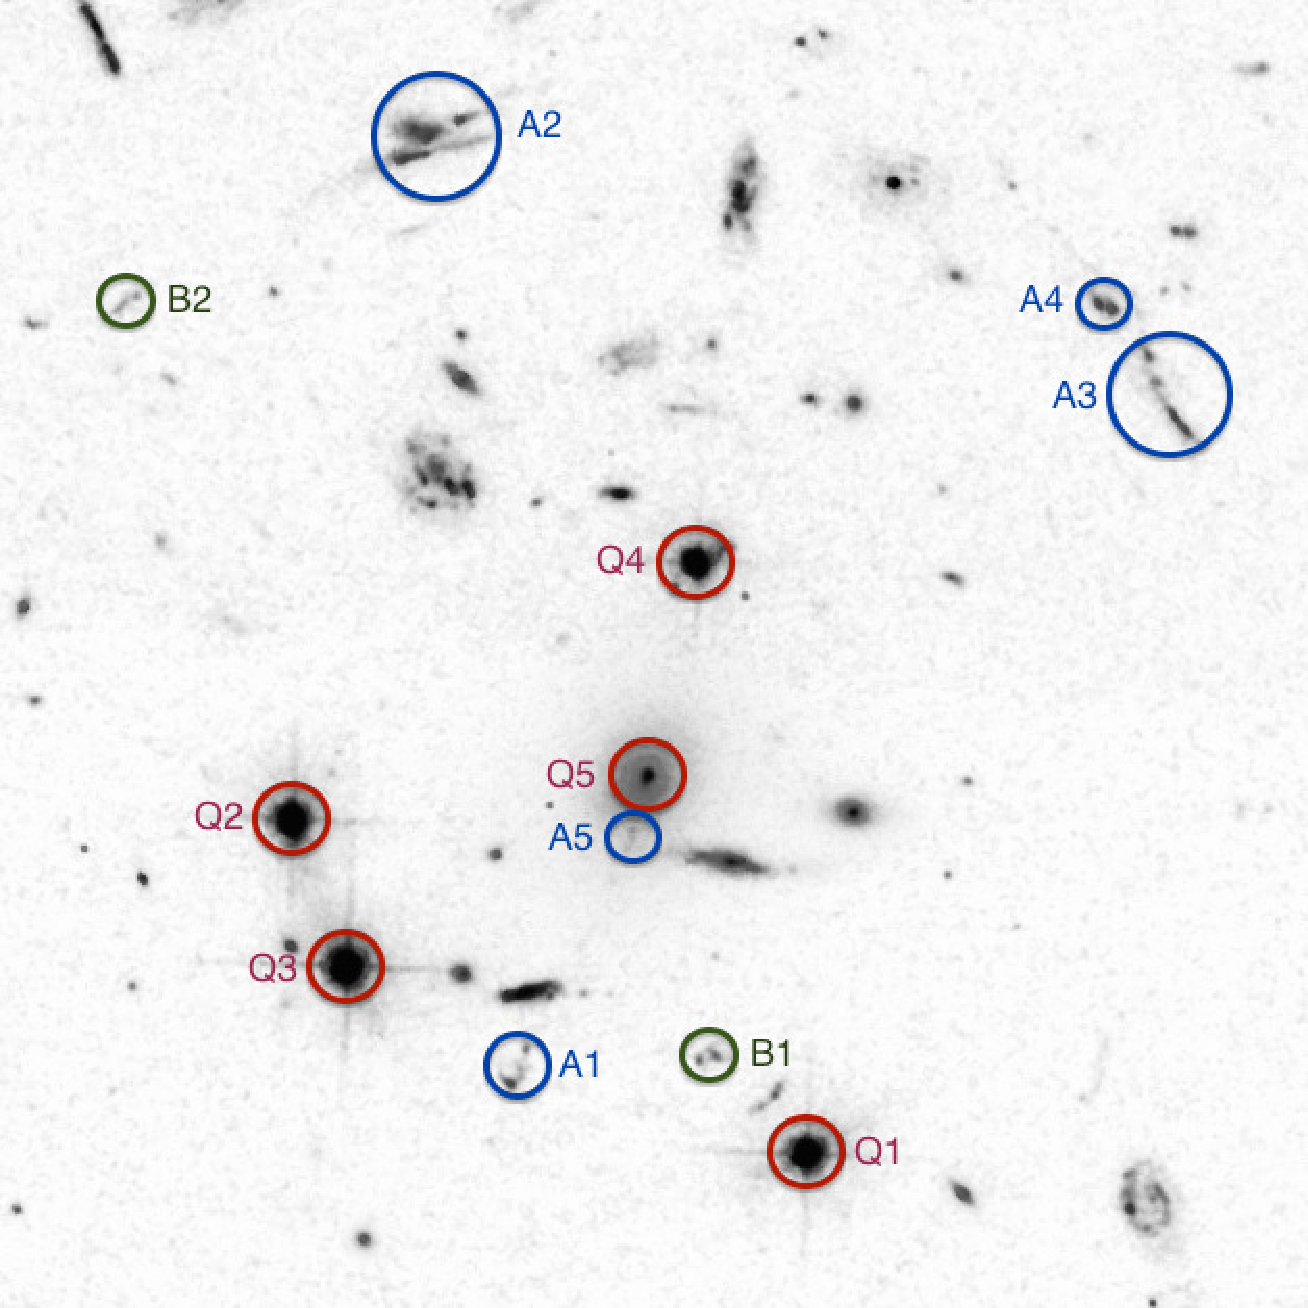
\includegraphics[width=0.45\textwidth]{figures/p4-figures/quasar.pdf}
\caption{Multiple images of the quasar, labelled Q1 to Q5 (red) in order of
  time delay (measured or expected). Showing galaxy A and B images in blue and green respectively. }
\label{p4:fig:raw}
\end{figure}

The Q system is natural for time-delay measurements.  Two of the four
possible time delays (between Q1-Q2 and Q1-Q3) of the quasar images
have been measured \citep{2007ApJ...662...62F,2008ApJ...676..761F} and
a third is expected.  The image separation is large (up to $14''$),
and since time delays scale with the square of the image separation,
the time delays are much longer than with galaxy lenses.  Image Q3
lags the nearby Q2 by 40 days and lags Q1 by 821 days.  The cluster
gas has also been observed in X-rays \citep{2006ApJ...647..215O}.  As
data have accumulated, many different models have been published
\citep{2004ApJ...605...78O,2004AJ....128.2631W,2006PASJ...58..271K,
  2007ApJ...663...29S,2008PASJ...60L..27I,2009MNRAS.397..341L,2010PASJ...62.1017O}.

\begin{figure}
\centering
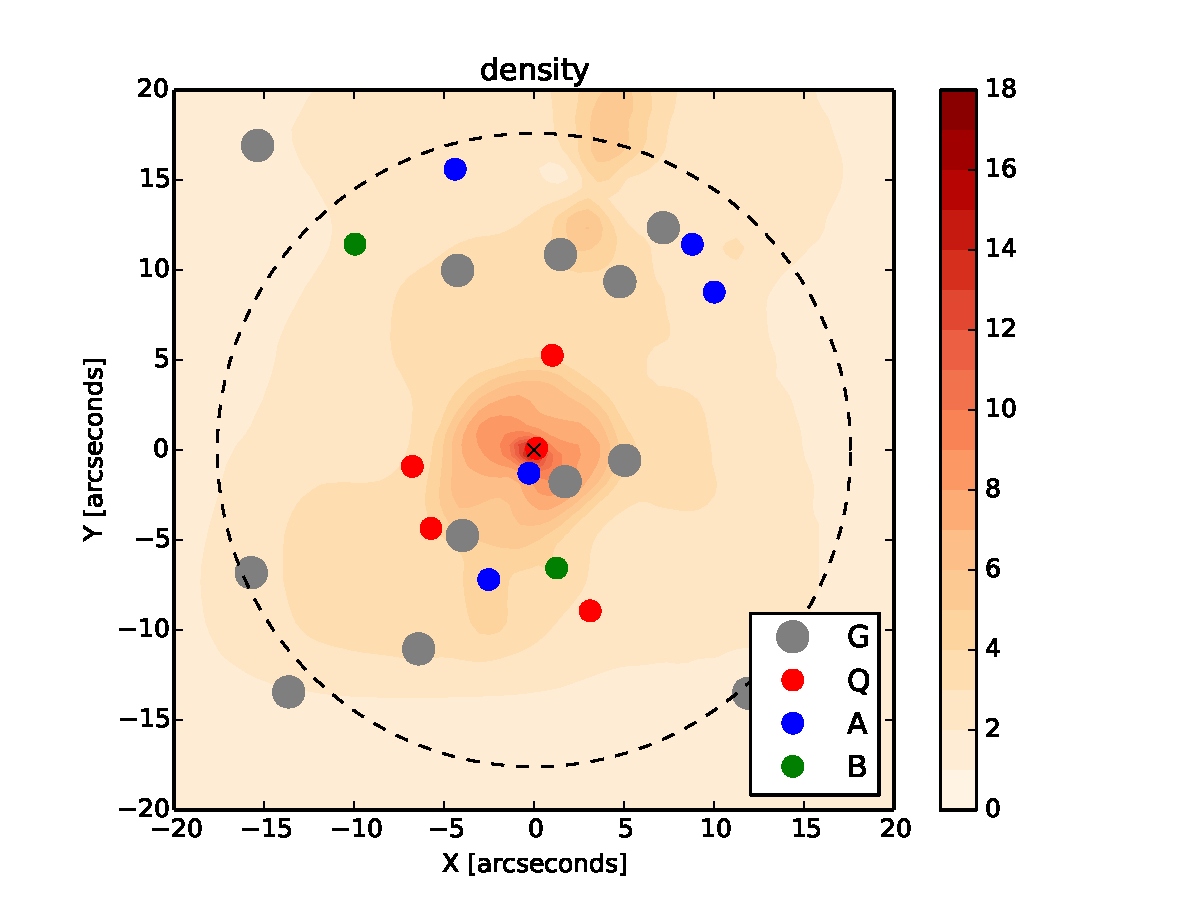
\includegraphics[width=0.49\textwidth]{figures/p4-figures/densityTD.pdf}
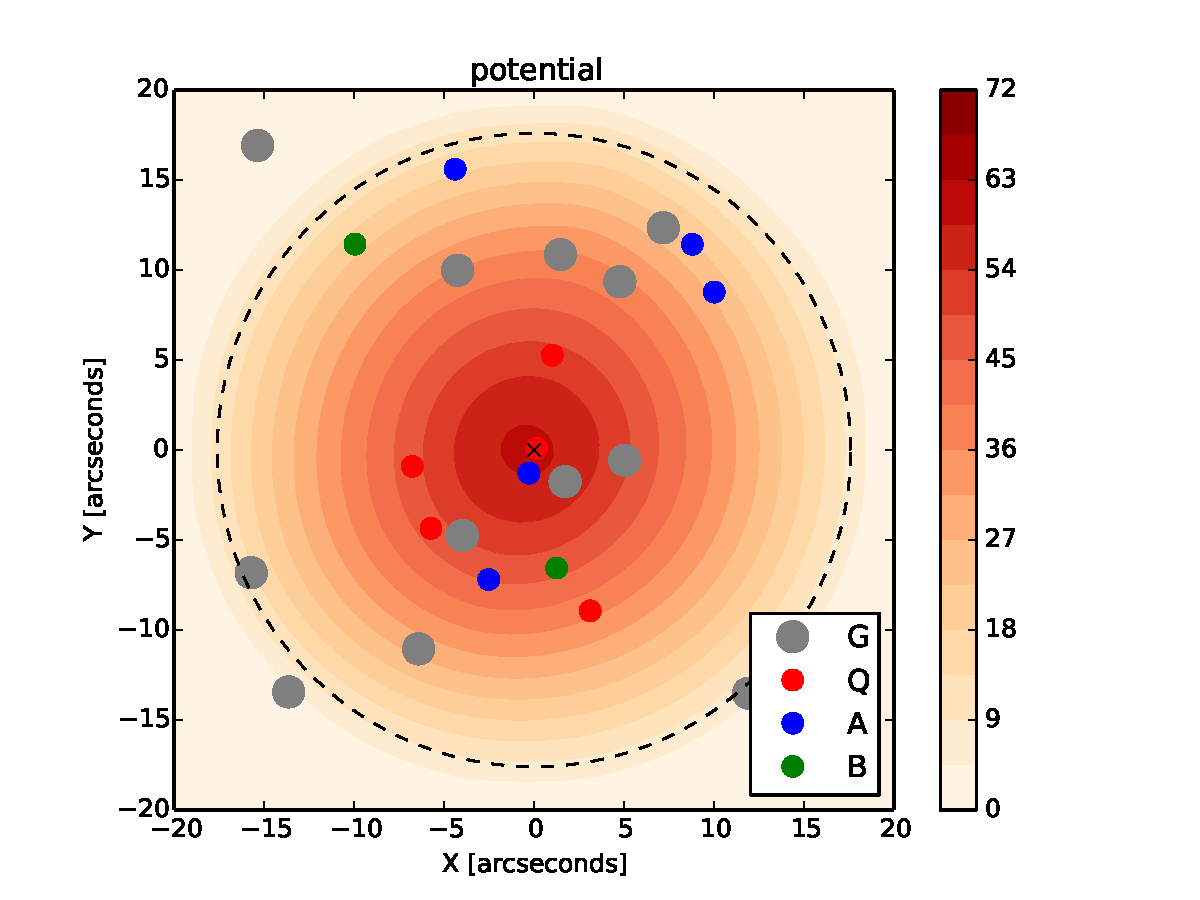
\includegraphics[width=0.49\textwidth]{figures/p4-figures/potentialTD.pdf}
\caption{The reference model (equation \ref{p4:eq:refmodel}) using all
  the data constraints.  Density (left panel) means projected density
  in $\rm kg\,m^{-2}$ and potential (right panel) is $t_{\rm grav}$ in
  years.  Lensed images and cluster galaxies are marked.}
\label{p4:fig:ref}
\end{figure}

\section{Time delays in lensing}

Let us briefly recall the physics of time delays.  This is
conveniently done using Fermat's principle as applied to gravitational
lensing \citep{1986ApJ...310..568B}.  Consider a sky-projected density
$\Sigma(\vec x)$ at redshift $z_L$.  Here $\vec x$ represents the physical
(not comoving) coordinates perpendicular to the line of sight.  The
gravitational time delay due to this mass will be
\begin{equation}
\nabla^2 t_{\rm grav} = -(1+z_L)\frac{8\pi G}{c^3} \, \Sigma(\vec x\,) \,.
\end{equation}
Now consider a source at $\vec x_s$.  A light ray coming from this
source, being deflected at the lens so that it heads to the observer,
will have an additional geometrical time delay of
\begin{equation}
t_{\rm geom} = \frac{(1+z_L)}{2c} \frac{d_S}{d_L d_{LS}}
               \left| \vec x - \vec x_s\right|^2
\end{equation}
where the $d_L$ is the angular-diameter distance to the lens, and $d_S$
and $d_{LS}$ are angular diameter distances from observer to source
and from lens to source respectively.  In a flat cosmology
\begin{equation}
d_{z_1,z_2} = \frac{c/H_0}{1+z_2}\int_{z_1}^{z_2}
              \frac{dz}{\sqrt{\Omega_m(1+z)^3 + \Omega_\Lambda}}
\end{equation}
gives the various angular-diameter distances.

The total time delay is then
\begin{equation}
t(\vec x, \vec x_s) = t_{\rm geom}(\vec x,\vec x_s) + t_{\rm grav}(\vec x) \,.
\end{equation}
Images will form where $t(\vec x, \vec x_s)$ has a minimum, saddle
point, or maximum.  The tensor magnification is the inverse matrix of
second derivatives of $t(\vec x)$.  Note that the dependence on $\vec
x_s$ has been differentiated out.  Flexion consists of the derivatives
of the tensor magnification, hence third derivatives of the time.

Lens modelling consists of reconstructing $\Sigma(\vec x)$ and $\vec
x_s$.  For a quasar source, $\vec x_s$ is a single point, for an extended
source a superposition of source points must be considered.
The earliest detailed lens models \citep{1981ApJ...244..736Y} already
noted the non-uniqueness of lens models. \cite{1985ApJ...289L...1F}
quantified the most important of these, now known as the steepness
degeneracy or the mass-sheet degeneracy: steeper mass profiles give
longer time delays, while leaving image positions and shapes the
same. As modellers explored models further, it turned out that the
shape of the mass distribution also affects time delays
\citep{1997MNRAS.292..148S,2003ApJ...582....2Z,2006ApJ...653..936S}.
Degeneracies have also been studied theoretically \citep{2013A&A...559A..37S}.
Having sources at multiple different redshifts (high redshift
contrast) tends to suppress degeneracies
\citep{1998AJ....116.1541A,2009ApJ...690..154S} but does not eliminate
them completely \citep{2008MNRAS.386..307L,2012MNRAS.425.1772L}.

It is useful to break down lensing time delays into three factors:
lens substructure, lens size and cosmology.  The time delay between
the innermost and outermost images can be written as
\begin{equation}
   \Delta t_{\rm in,out} = f_{\rm lens} \frac{A_{\rm lens}}{A_{\rm
       sky}} \, \frac{d_Ld_S}{d_{LS}} \quad
A_{\rm lens} = \frac\pi4 (\theta_{\rm in}+\theta_{\rm out})^2 .
\end{equation}
Cosmology enters through the distance factors, while $A_{\rm lens}$ is
the size of the lens on the sky, and is fixed by the astrometry.  With
these factors fixed, $f_{\rm lens}$ is the remaining dependence on
substructure.  Typical values are 2--6 for systems with 2+1 images,
and 0.5--2 for systems with 4+1 images \citep{2006ApJ...650L..17S}.
That is to say, substructure is very important for time delays.  This
dependence is undesirable when estimating cosmological parameters, but
it is welcome for inferring substructure.

\section{Isolating the time-delay modes}\label{p4:sec:theory}

In this section we produce a form of principal components analysis
(PCA) to isolate the information that time delays provide on the mass
distribution, assuming the cosmological parameters are known. A
somewhat related technique, for lensing clusters with multiple source
redshifts but not necessarily including time delays, is developed by
\cite{2014MNRAS.437.2461L}.

We reconstruct the mass distribution in two ways: first, including the
measured time delays (say TD models), and second, with no time-delay
information (say NTD models).  For each of TD and NTD, we
reconstructed an ensemble of mass maps (30 in number).  Each mass map
is on a grid (size $74\times 74$).

We now wish to find the variation present in the NTD ensemble but not
in the TD ensemble.  This will provide information on substructure
possibilities left by image data (only) but ruled out by time delays.
Let $X_n^i$ denote the projected density of the $i$th TD model ($i$
going from 1 to 30 in this paper) at the $n$th grid point (of
$74^2=5476$ grid points).  Similarly use $Y_n^i$ for the NTD mass
maps.  Next, we choose a reference $Z_n$,
\begin{equation} \label{p4:eq:refmodel}
  Z_n = \langle X_n^i \rangle
\end{equation}
which is the ensemble average of the TD maps.  Then
\begin{equation}
  \Delta X_n^i = X_n^i - Z_n
\end{equation}
is the ensemble variation about the reference.  Then we introduce
a moment matrix
\begin{equation}
  M_{mn}(X) = \left\langle \Delta X_m^i \, \Delta X_n^i \right\rangle
\end{equation}
where the average is again over the TD maps.  $M_{mn}(X)$ is just the
covariance between pairs of grid points.  The eigenvalues and
eigenvectors of $M_{mn}(X)$ describe how sets of grid points tend to
vary together.  Let us denote them by $\lambda_k(X)$, and $V_n^k(X)$
respectively; the superscript $k$ denotes the $k$th eigenvalue and
eigenvector ($k=1$ having the largest eigenvalue).  In practice, the
first few eigenvalues dominate.  The vector
\begin{equation}\label{p4:eq:TD}
   Z_n \pm \sqrt{|\lambda_k(X)|} \, V_n^k(X),
\end{equation}
displayed as a density map, shows the principal mode of variation of
the mass model.  (There is no sum over $k$.)  These variation modes
are, of course, orthogonal.

We then proceed to the NTD maps. Let these be $Y^i_n$ and let
\begin{equation}
  \Delta Y_n^i = Y_n^i - Z_n
\end{equation}
be the variations with respect to the reference model.  We now
subtract off the variation modes of TD mass maps
\begin{equation}
   \Delta \bar Y_n^i = \Delta Y_n^i - \sum_{k}
   \left( {\textstyle\sum_m} \Delta Y^i_m V_m^k(X) \right) V_n^k(X)
\end{equation}
leaving variations that are orthogonal to the TD
variations.  Using these, we build another moment matrix
\begin{equation}
  M_{mn}(Y) = \left\langle \Delta \bar Y_m^i \, \Delta \bar Y_n^i \right\rangle.
\end{equation}
The eigenvalues and eigenvectors of $M_{mn}(Y)$ contain the modes
present in NTD maps models but absent from the TD maps.  These modes
can be conveniently displayed as
\begin{equation}\label{p4:eq:NTD}
   Z_n \pm \sqrt{|\lambda_k(Y)|} \, V_n^k(Y).
\end{equation}
We call these ``variations ruled out by the time delays'' and these
are the main results of this paper.  One sign of the $\pm$ must be
chosen for definiteness, but it does not matter which one.

\begin{figure}
\centering
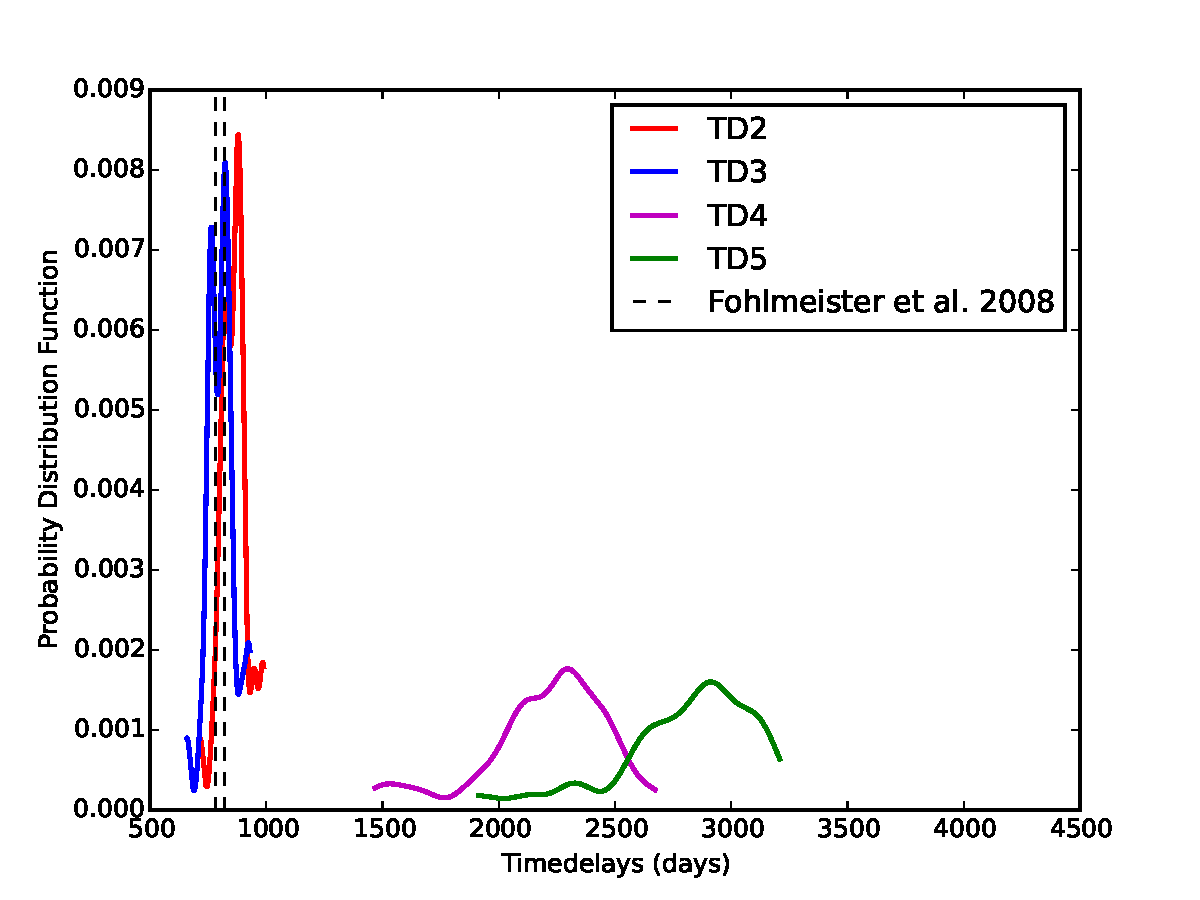
\includegraphics[width=0.49\textwidth]{figures/p4-figures/timedelay_hist_TD.pdf}\\
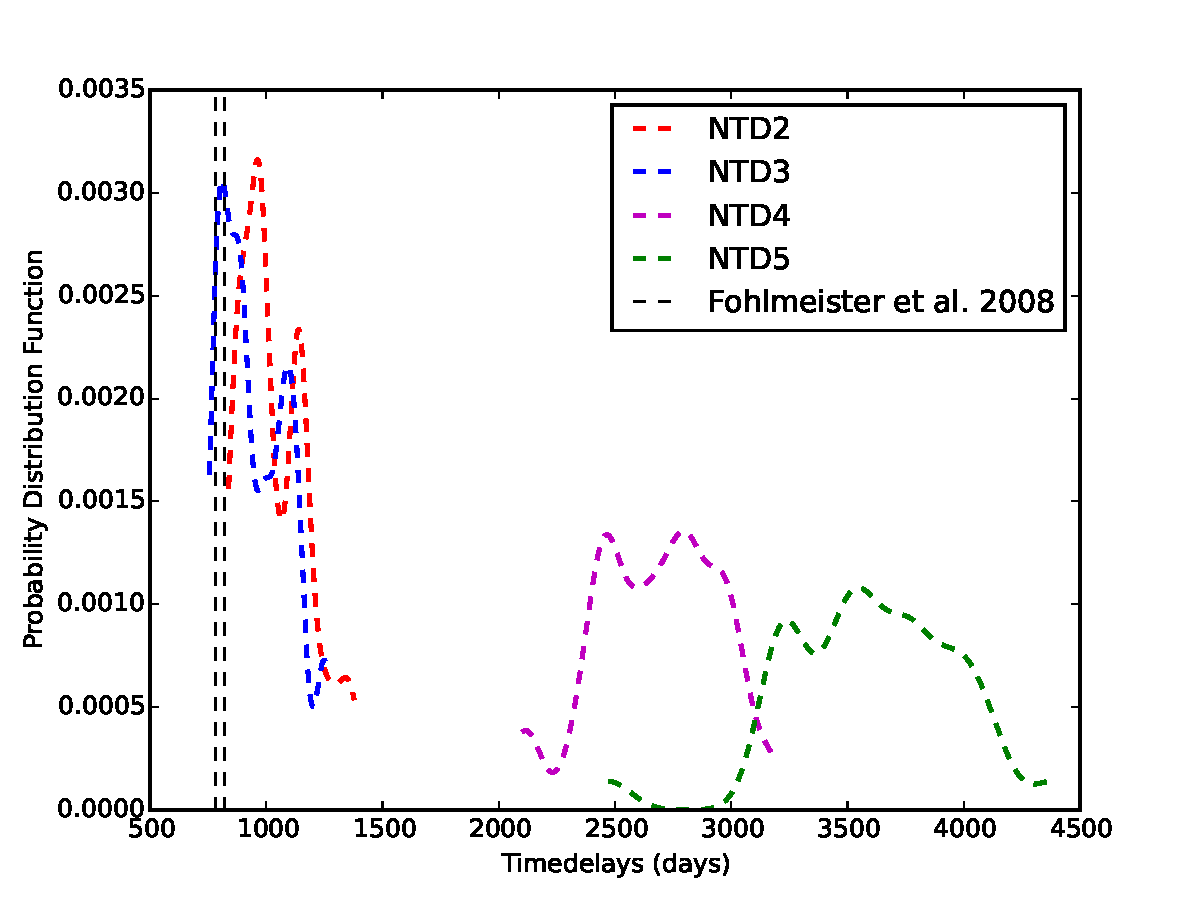
\includegraphics[width=0.49\textwidth]{figures/p4-figures/timedelay_hist_NTD.pdf}
\caption{Time delay estimates using TD models (upper) and NTD models
  (lower).  TD2, TD3, TD4 and TD5 (or NTD2, NTD3, NTD4, NTD5) are 
  the time delays for image Q2, Q3, Q4 and Q5
  respectively with respect to Q1.  Vertical dashed lines show the
  input time delays from \cite{2008ApJ...676..761F}.}
\label{p4:fig:timedelays}
\end{figure}


\section{Application to SDSS J1004+4112}

The mass distribution $\Sigma(\vec x)$ can be reconstructed in
different ways: \cite{2010PASJ...62.1017O} uses a parametrized form,
\cite{2007ApJ...663...29S} built it out of mass tiles or pixels, while
\cite{2009MNRAS.397..341L} used an adaptive superposition of Plummer
components.  The latter, and in particular the GRALE code, is used
in the present work.

\subsection{Mass reconstruction using GRALE}\label{p4:sec:grale}

As mentioned above, GRALE
\citep{2006MNRAS.367.1209L,2007MNRAS.380.1729L,2009MNRAS.397..341L}
makes free-form mass models for the lensing cluster, as a
superposition of many Plummer lenses.  Except for the redshift and 
general location, no information from the lens itself is used.
The inversion input consists of (1)~lensed-image
positions and source redshifts, (2)~regions where additional images
have not been identified but could be present, and (3)~time delays if
any.  Each of these is used to define a fitness measure of a mass
distribution.

\begin{itemize}
  \item For a given mass map, the input multiple images are ray-traced
    back to the source plane.  The `overlap fitness' of the mass map
    expresses how well these back-projected images overlap.  It is
    important to consider fractional overlap rather than simple
    source-plane distances to avoid favouring extreme magnification
    (tiny sources).
  \item The back-projection may give rise to extra images.  If they
    are not in regions specified by the modeller as allowed, they are
    spurious. These penalize the mass map through a `null fitness'
    measure.  Through the null fitness, GRALE uses the non-occurrence
    of images at random locations as useful data.
  \item The `time-delay' fitness measures how well the time delay in a
    mass distribution agrees with the observations.
\end{itemize}

GRALE uses a multi-objective genetic algorithm to find free-form mass
maps which provide optimal fits to the data according to the above
criteria.  If more Plummer-lens components are allowed, the fitness
will tend to be better.  Accordingly, we used a heuristic
Occam's-razor criterion to find a compromise between better fitness
and more components \citep{2014MNRAS.439.2651M}.  This effect sets the
resolution adaptively.  No additional priors or regularization are
used.

\subsection{Mass models}

Our mass maps for SDSS J1004+4112 were of two kinds, as follows.
\begin{itemize}
\item No time delay (or NTD) models.  We used the three image systems
  (Q, A and B; total 12 images), but gave no time-delay information in
  this case. GRALE finds an optimal solution, restricting extra images
  using the technique of null spaces, for this dataset. We repeated
  the same procedure 30 times to generate a statistical ensemble of 30
  models.
\item Time delay (or TD) models.  For these we used the same data set,
  plus the two measured time delays: 40 days in Q2--Q3 and 821 days in
  Q1--Q3 (see Figure \ref{p4:fig:raw}).  Following the same procedure, we
  made an ensemble of 30 mass maps. Figure \ref{p4:fig:ref} shows the
  ensemble average of the TD models, which is used as the reference
  $Z_n$ from Section \ref{p4:sec:theory}. The left panel of Figure
  \ref{p4:fig:ref} shows the projected density and the right panel shows
  the potential in the colour code. This mass distribution shows slight
  differences from \cite{2009MNRAS.397..341L}, because the present
  work uses an adaptive resolution scheme, but these differences do
  not appear to be significant.
\end{itemize}

The method described in Section \ref{p4:sec:theory} is then applied to
the TD and NTD models.  Tests in \cite{2014MNRAS.439.2651M} indicate
that GRALE ensembles of this size underestimate the actual
uncertainties by a factor of two, but do explore the different
uncertainties.  Thus, the eigenvalues reported below are certainly
underestimates, but the eigenvectors should be a good representation
of the variation.

\begin{figure}
\centering
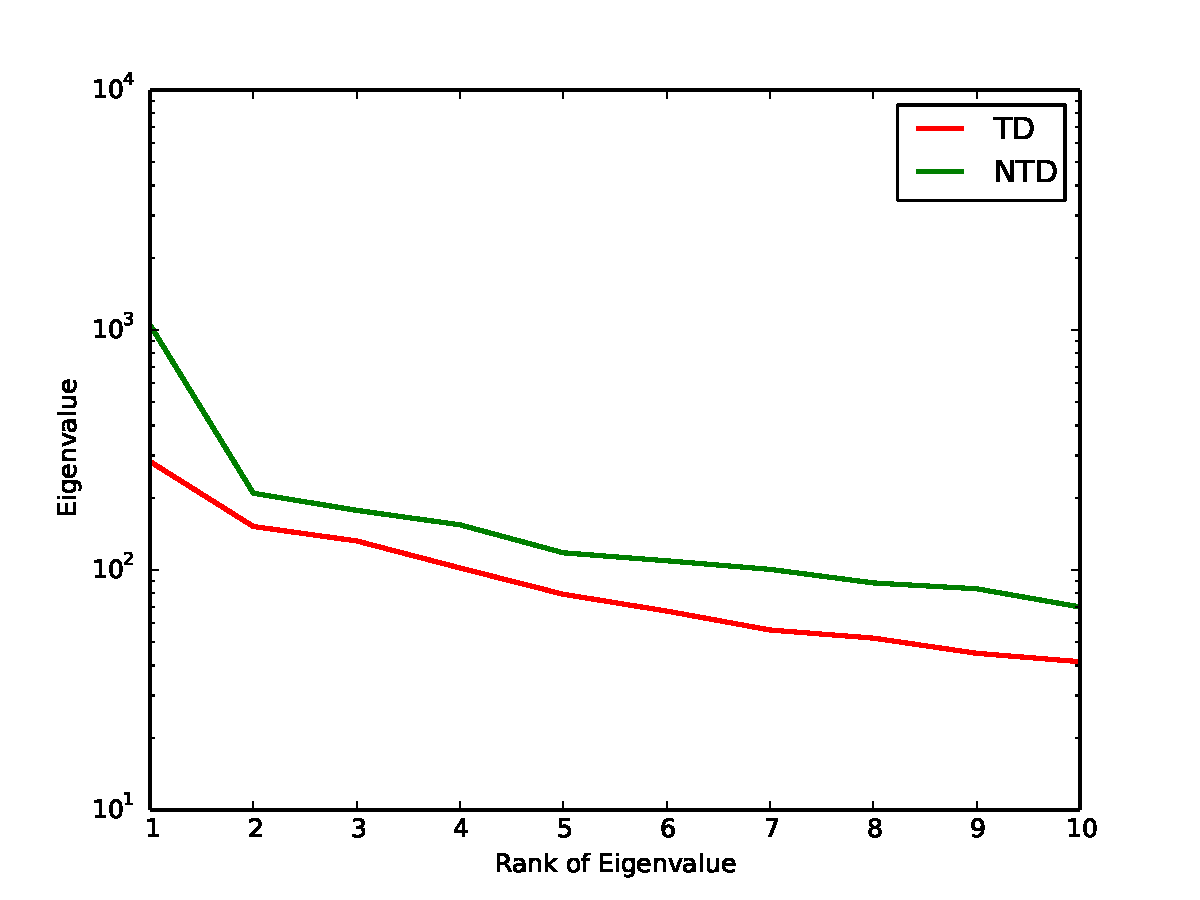
\includegraphics[width=0.49\textwidth]{figures/p4-figures/eigval.pdf}
\caption{Distribution of eigenvalues $\lambda_k(X)$ and
  $\lambda_k(Y)$, labelled as TD and NTD respectively, ranked by
  absolute value.}
\label{p4:fig:eigvals}
\end{figure}

\begin{figure}
\centering
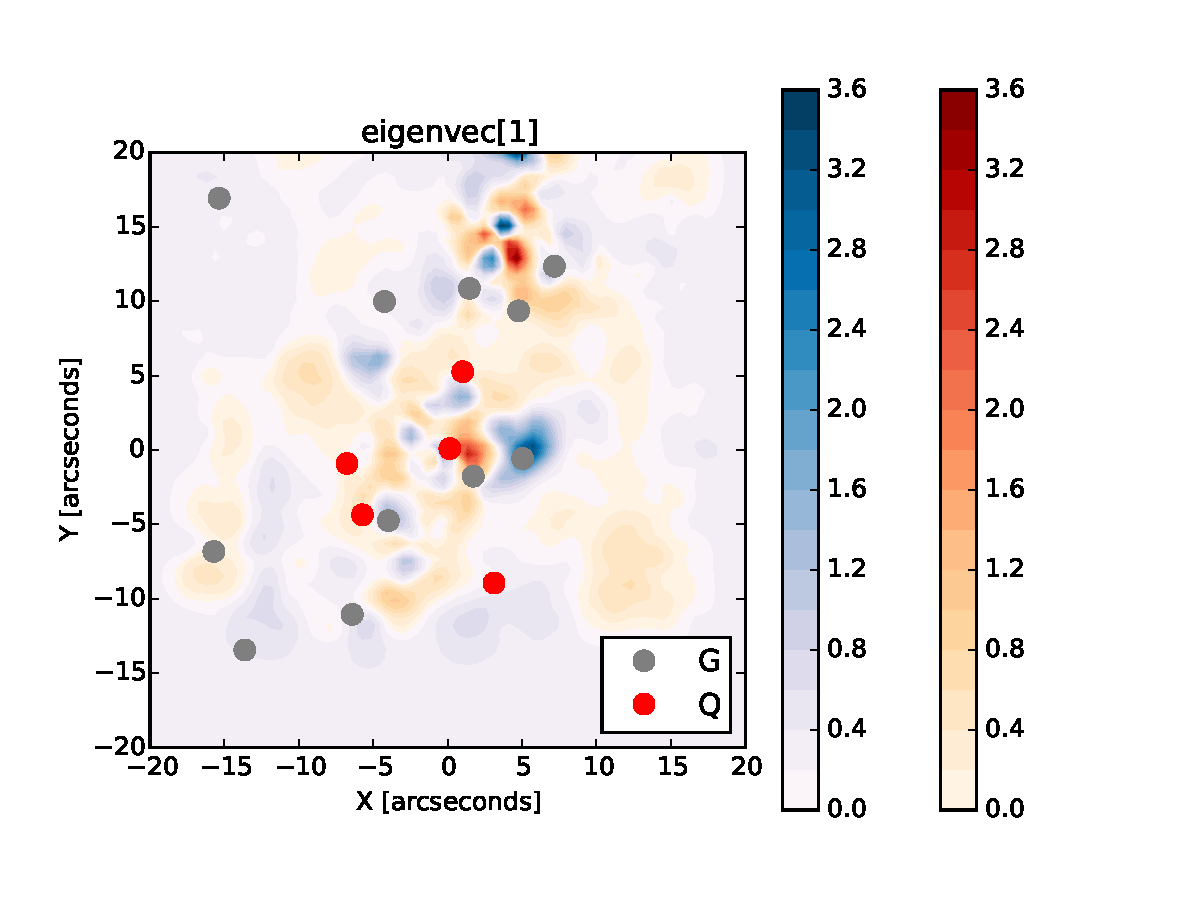
\includegraphics[width=0.99\textwidth]{figures/p4-figures/density+eigenvec1NTD.pdf}
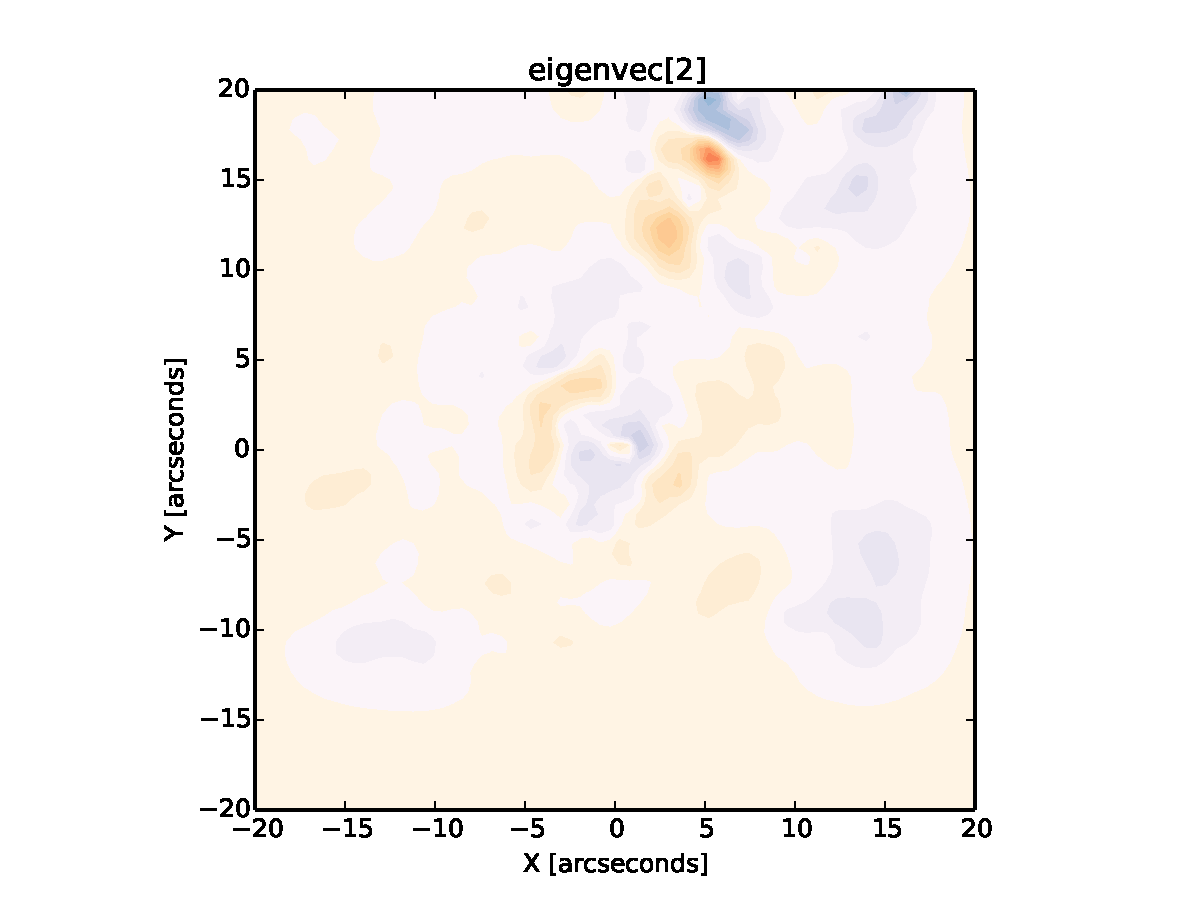
\includegraphics[width=0.49\textwidth]{figures/p4-figures/density+eigenvec2NTD.pdf}
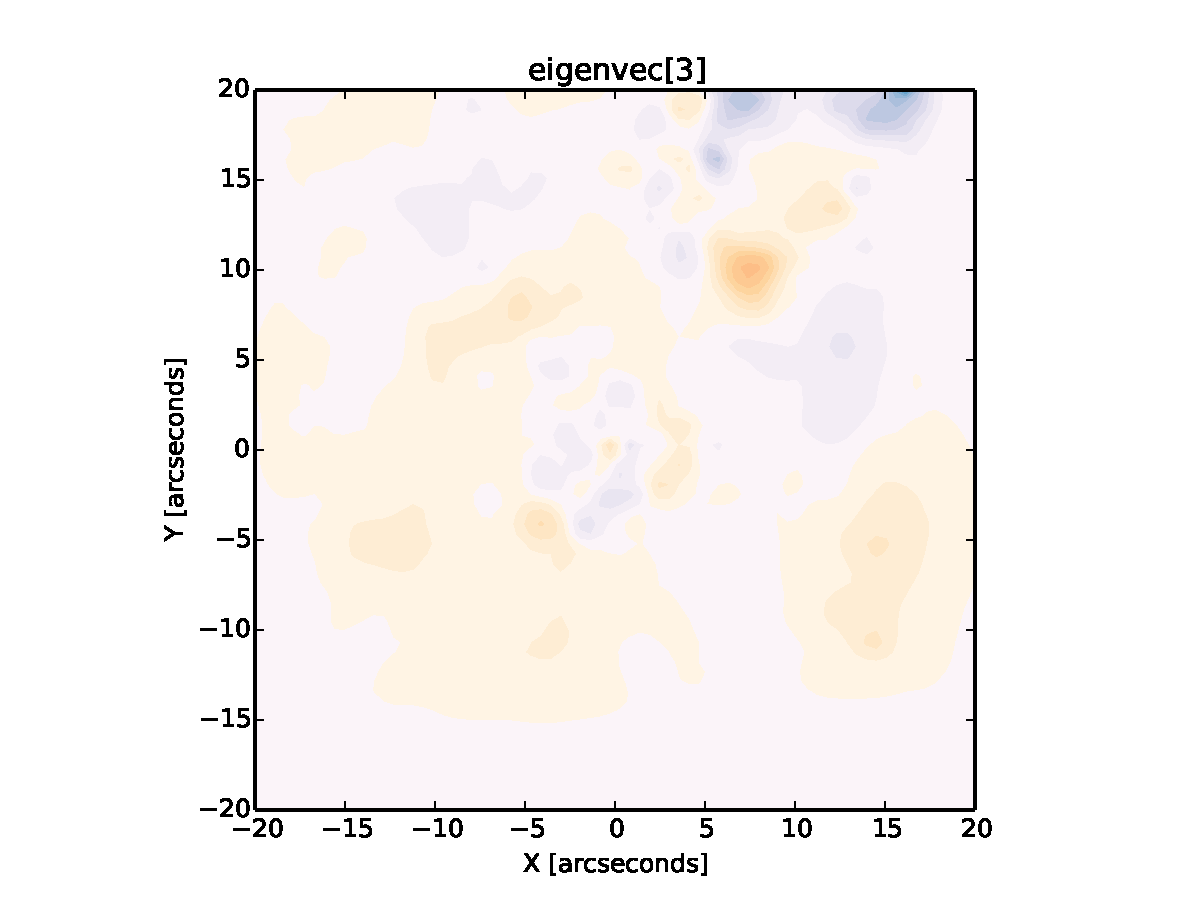
\includegraphics[width=0.49\textwidth]{figures/p4-figures/density+eigenvec3NTD.pdf}

\caption{The main/largest variation in surface density
  ruled out by time delays (upper
  panel). The red and the blue color bars represents positive and
  negative values (in $\rm kg\,m^{-2}$) respectively.  The two lower
  panels show the second and third largest variation ruled out by time
  delays.}
\label{p4:fig:mainmode}
\end{figure}

\begin{figure}
\centering
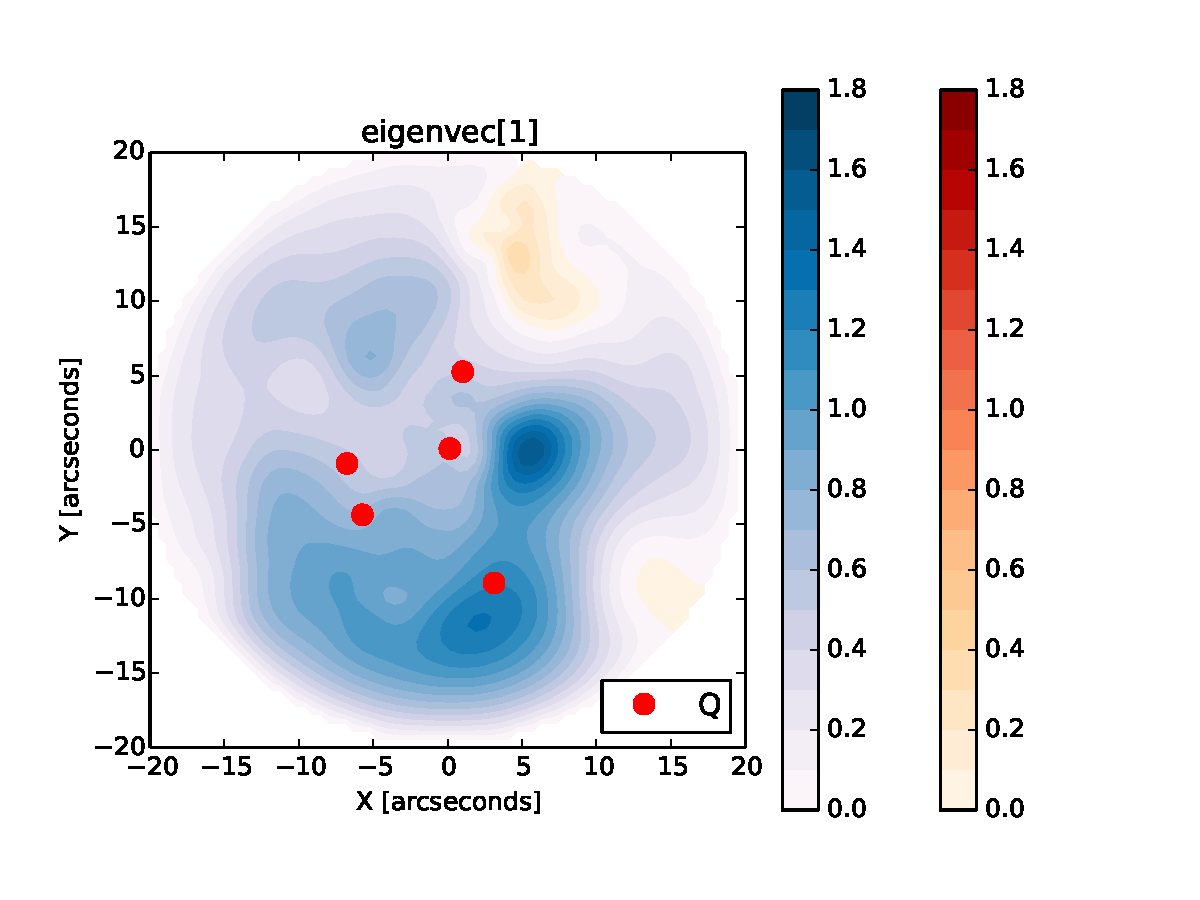
\includegraphics[width=0.99\textwidth]{figures/p4-figures/potential+eigenvec1NTD.pdf}
\caption{The main/largest variation ruled out by time delays. The red
and the blue colour bars represents positive and negative values (in years) respectively. }
\label{p4:fig:mainmode-potential}
\end{figure}

\subsection{Results and interpretation}

Figure \ref{p4:fig:timedelays} shows the distribution of time delays in
the TD and NTD ensembles.  As expected in the TD models, the first two
time delays, which were also used as data inputs, show little
variation (though larger than the observational uncertainties) while
the other two show large variations.  In the NTD models, all the time
delays show large variations.  Most of the TD models also favour lower
time delays for Q4 and Q5, as compared to the NTD models estimate.  Thus,
existing time-delay measurements constrain future measurements to some
degree, but not very tightly, indicating that future measurements will
bring substantial new information.

Figure \ref{p4:fig:eigvals} shows the eigenvalues of the NTD and TD
modes.  The largest NTD mode evidently dominates, being a factor of
five larger than the second largest mode.  When time delays are
included, it is also the case that one TD mode is much larger than the
rest.

\begin{figure}
\centering
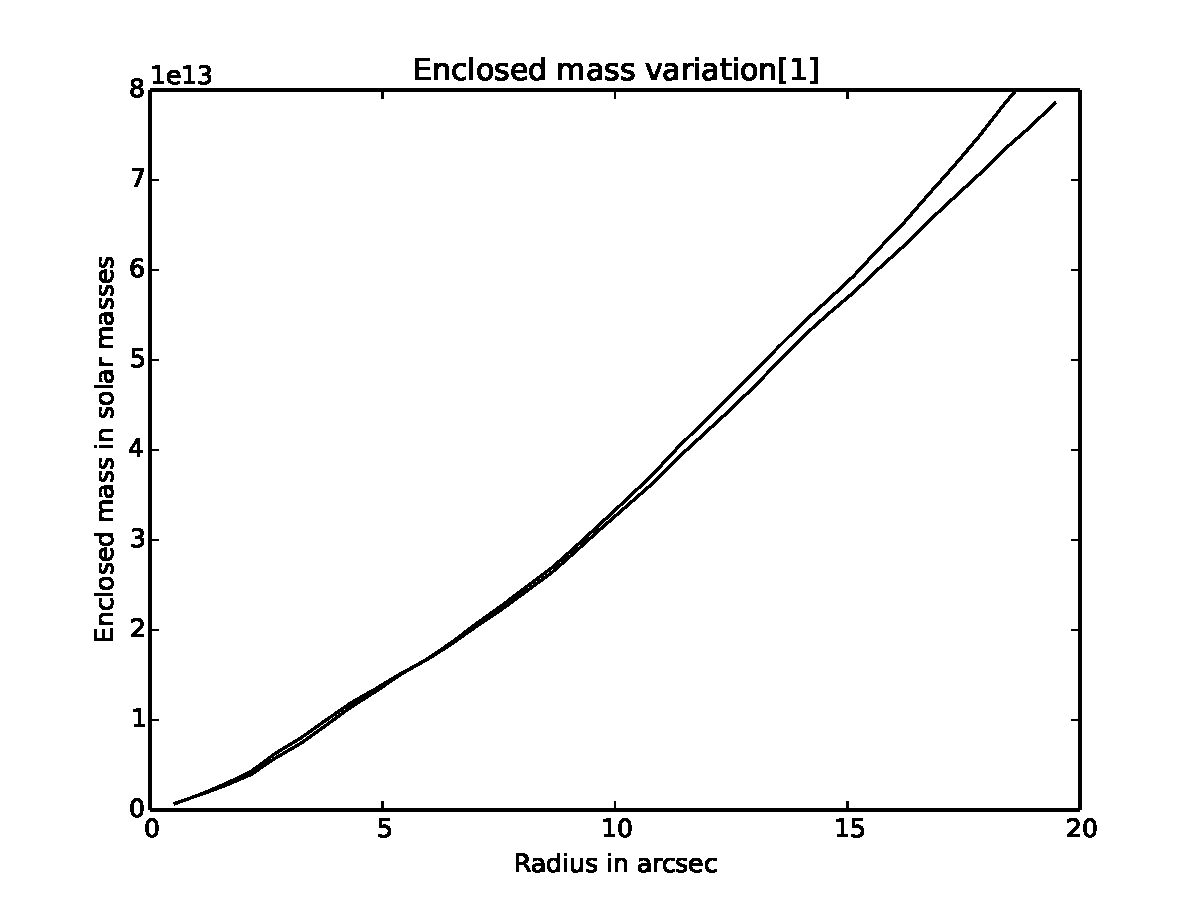
\includegraphics[width=0.49\textwidth]{figures/p4-figures/massenc_linear1.pdf}
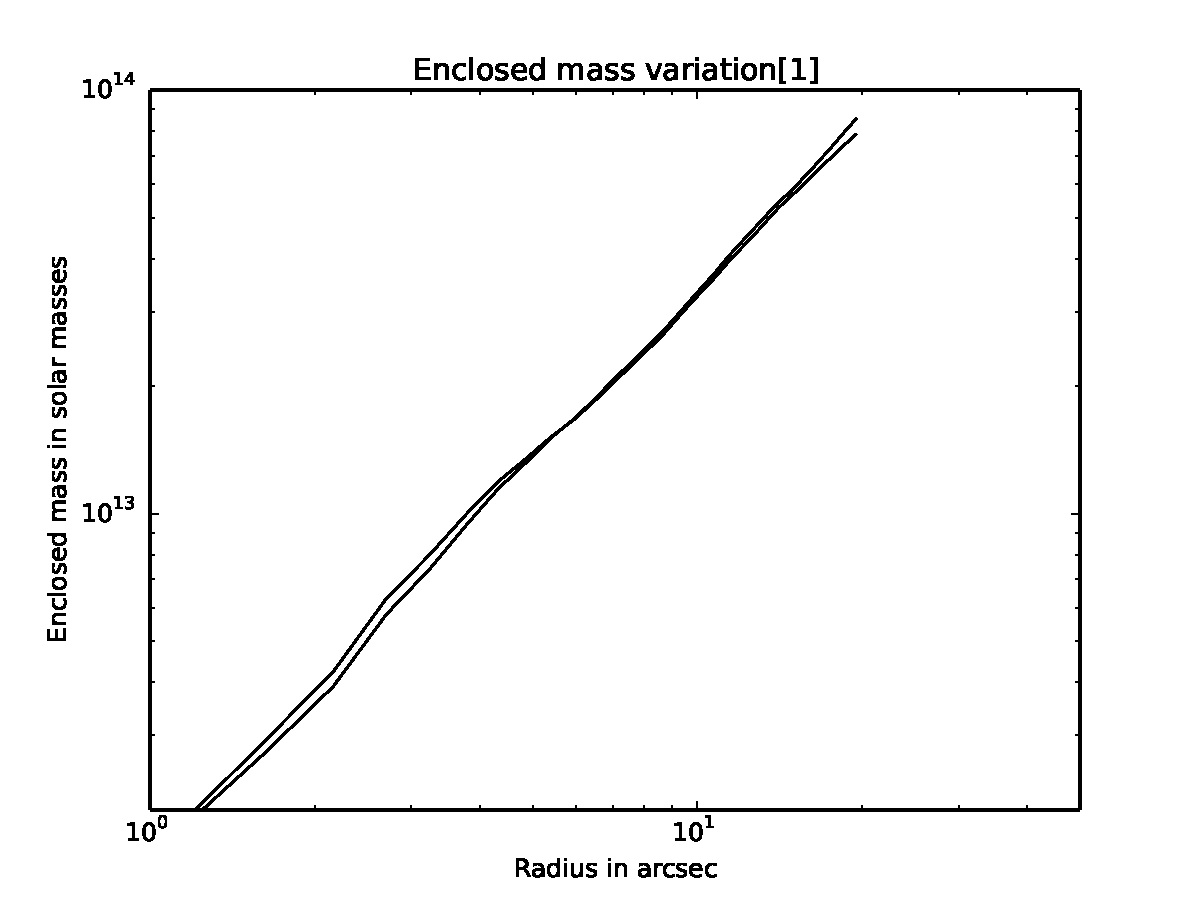
\includegraphics[width=0.49\textwidth]{figures/p4-figures/massenc_log1.pdf}
\caption{Variation of enclosed mass of the reference model around the 
largest NTD mode (shown in Figure \ref{p4:fig:mainmode}) as a function of 
projected radius.  Linear scales on the left, log scales on the right.}
\label{p4:fig:mainmode-menc}
\end{figure}

Figure \ref{p4:fig:mainmode} presents the main result of this paper.  It
illustrates the largest NTD variation mode that is absent in the TD
ensemble (cf.\ equation \ref{p4:eq:NTD}), in other words, the largest
variations ruled out by the time-delay measurements.  The upper panel
of the figure shows the eigenvector corresponding to the largest
eigenvalue.  The two central blobs in the upper panel of Figure
\ref{p4:fig:mainmode} (blue and red, hence anti-correlated) allow the
mass to shift the local mass peak towards or away from the cluster
centre, and hence change the steepness of the mass profile. Without
the TD constraints, the central peak of the mass distribution can be
 more lopsided, whereas the TD constraints force the central peak to
be rounder.  The rather large uncertainties (20\%--40\% in $\Sigma$)
in the central region of the NTD models is reduced in the TD
models. This local uncertainty of 20\%--40\% is, however, less than
1\% of the total mass in the strong-lensing region.  That is to say,
time delays are constraining substructures that are only a percent of
the total.  The red and blue blobs also are in the vicinity of
the two galaxies in the very central region.  That may be coincidental,
but it is worth remarking that the mass in the blobs is of the order of a
galaxy-halo mass, such as may be tidally stripped from a galaxy near
the centre of a cluster.  This suggests that time delays may give very
sophisticated information about the variation of the mass near the
environment of the galaxies in the central region, or in other words,
about the sub-structures in a dense environment. Therefore, the third
time-delay, which is expected for the image Q4, could be very useful
in extracting the substructure information of the cluster near its
centre.  Note that this interesting region is not accessible through
the more well-known techniques of weak lensing and flexion.

The lower two panels of Figure \ref{p4:fig:mainmode} shows the second and
third largest variation modes. These variations modes are weaker,
also evident from Figure \ref{p4:fig:eigvals} as all other
eigenvalues after the first one are sub-dominant.  The number of
non-zero eigenvalues for NTD should equal the number of time-delay
measurements (two in this case), but in practice further modes are
present, and only gradually die away.  These are basically noise
modes, which exist because we have only 30 models for our
principal-components analysis.  (Numerical noise due to round-off
error in the matrix operations is negligible.)

Upon measuring the short Q2-Q3 time delay \cite{2007ApJ...662...62F}
already noted that substructure would be necessary to account for
their observation.  We have not considered separately the case where
only this one time delay is known.  We see in
Figure~\ref{p4:fig:eigvals}, however, that only one of the NTD
eigenvalues is larger than the TD eigenvalues, indicating that only
one of the measured time delays (surely the longer Q1-Q3 value) gives
a substructure constraint.  This does not mean that the Q2-Q3
measurement can be explained without substructure; only that the
measurement on its own is not constraining what that substructure
could be.

Figure \ref{p4:fig:mainmode-potential} shows the variation in lens
potential $t_{\rm grav}$ corresponding to the density variation from
the main panel in Figure \ref{p4:fig:mainmode}.  Here we can see the
effect of measuring the delays between Q1, Q2, and Q3.  The NTD models
have $t_{\rm grav}$ between Q1 and Q2 varying by about 0.5 years, that
is, varying by 25\% of the measured value.  Between Q2 and Q3, the
time delay varies by about 0.3 years in the NTD models, which is more
than twice the measured delay between this pair.  Between Q3 and Q4
there is little variation.  This does not mean that the NTD models
have little variation in the Q3--Q4 delay; it just means that similar
variation is present in the TD models, and hence not ruled out by the
Q1--Q2--Q3 measurements.  All this is what one would have expected
from Figure \ref{p4:fig:timedelays}.  Surprising, however, is that the
largest variation ruled out by the time delays is the blob $5''$ west
of the cluster centre, not near any of the images.

Figure \ref{p4:fig:mainmode-menc} shows the enclosed mass and its
variation.  The enclosed mass is comparable with Figure~3 of
\cite{2010PASJ...62.1017O}, as expected.  As also evident from figure
\ref{p4:fig:mainmode}, the NTD mode is not like a global change of steepness --- the
steepness appears to have been already constrained by the image data,
because of the redshift contrast between the Q, A and B systems.  So
the time delays are giving us information not on the steepness but
about the shape of the profile.  The NTD models allow for strongly E/W
ellipticity in the central region, changing to a more N/S elongation
further out, but the time delays force the model to be rounder and
less lopsided.

\section{Discussion}

This paper expresses the information that comes from lensing time
delays in a way that is orthogonal to other lensing observables.  We
used the cluster SDSS J1004+4112 because of the richness of
strong-lensing information.  SDSS J1029+2623
\citep{2013ApJ...764..186F,2013MNRAS.429..482O} would also be
interesting for a similar study, as would MACS J1149+2223
\citep{2014arXiv1411.6009K,2014arXiv1411.6443O} if time delays for the
recently-discovered supernova can be measured.  The main results are
shown in figures \ref{p4:fig:mainmode} and \ref{p4:fig:mainmode-potential}.
The interpretation is very preliminary, because a new time delay is
expected soon, but nonetheless shows two interesting features.

First, it is remarkable how a small mass redistribution can produce a
large difference in time delays.  As Figure \ref{p4:fig:mainmode} shows,
the main mass-redistribution ruled out by the two published time
delays is a small blob that is only $\sim1\%$ of the total mass in the
strong-lensing region, and yet this redistribution can change a time
delay by 50\%.  It appears that time delays are providing substructure
constraints at the 1\% level.  

Second, the mass redistribution is not mainly near the images, but
mainly in another region of the cluster.  Overall, the time delays
reduce the allowed lopsidedness of the cluster, but it is intriguing
that the main redistribution appears to shift mass from the
neighbourhood of one cluster galaxy to the vicinity of another cluster
galaxy.

The expected third time-delay measurement in this cluster will be very
interesting. As seen in Figure \ref{p4:fig:raw}, the two time delays we used
in our analysis are between Q1--Q2 and Q1--Q3. All of these images are
towards the west and south-east of the cluster.  The new measurement
would involve Q4, which lies to the north.

So, we conclude that strong lensing with time delays provides important
constraints on the distribution of matter near the centre of the
lensing cluster, regions not accessible to weak lensing or flexion.
Additionally, time delays may provide new information on the 
distribution of matter in the
densest regions of clusters and indirectly on the role of AGN feedback,
adiabatic contraction, and other dynamical processes.

%==============================================================================
% Chapter 6: Paper 5
%==============================================================================

\chapter{Quantifying Substructures in Hubble Frontier Field Clusters}
\label{p5:chap:hff-substructures}

\section{Introduction to the Paper}

Numerical simulations have provided an insight to the theory of structure formation. 
Large collapsed objects, like cluster of galaxies, form by a series of mergers of 
small mass systems, like galaxies or group of galaxies, and the associated gas, dark-matter
halos etc. The abundance of sub-structures in a merging system should be quantified 
to study the merging stage of the cluster. This evaluation is trivial using simulations. 
The observed macroscopic properties of galaxies and galaxy clusters, for example 
gas mass, bulge sizes
etc., can be well reproduced using the current generation hydrodynamical simulations. 
However, a more ambitious comparison would be the total mass distribution in the
clusters. As the total mass distribution in an ongoing merger is the result
of an initial random field evolved with deterministic forces, only statistical
properties can be derived, and not the actual distribution. The derived statistical
quantities like radial density profile, sub-structure mass function etc., can be
compared to those of the observed clusters to validate the simulation
ingredients. 

Tracing the mass distribution in observed clusters is a non-trivial task, as 
the mass is not an observable, which light is. Gravitational lensing, particularly
strong lensing, is an unbiased 
tool to estimate the total mass distribution. However, the resolution of the
reconstructed mass maps depends on the priors and the lensing data. In order to
have unbiased estimates, priors must be minimal, and the total mass distribution
must be inferred using lensing data alone. Therefore, we need non-parametric
mass reconstruction methods without light-traces-mass (LTM) assumption, and higher
density of lensed images of the background sources, in order to correctly model 
the mass distribution of the lens (or the cluster).

Such large quantity of lensing data have recently been provided by the Hubble Space
Telescope (HST) under the Hubble Frontier Field (HFF) discretionary program. The HFF 
consists of six massive clusters of galaxies in redshift range 0.3 to 0.5, each 
containing 200 lensed, along 
with the good estimates of their redshifts. 

In this paper, we produced mass models for the six HFF clusters using the pre-HFF
data, and a mass model using HFF data for one of them. We report the gain in the
spatial resolution of mass maps using HFF data over pre-HFF data. To make
these mass maps, we use GRALE, a strong gravitational lensing non-parametric 
mass reconstruction technique, without assuming any light information from
the clusters, except for the redshift. The mass distribution of all HFF
clusters show elongation, multiple-cores, and many sub-structures, 
indicating a recent major merger. Therefore, extracting radial profiles
of the clusters is not very encouraging. Also, because gravitational lensing
can only estimate the sky-projected 2D mass distribution, many sub-structures
are erased, and an estimate of the sub-structure mass function
cannot be derived without LTM assumption. 

We proposed the power spectrum of the 2D mass distribution as an estimator
for the sub-structure. We measured this quantity for all HFF clusters, and 
found large power at small scales for clusters at low redshift or with
larger number of lensed images. We made similar measurements of the
power spectrum from simulated clusters, both dark-matter only and 
hydrodynamical, and
found that the average power in simulated clusters is larger than that
in the observed clusters at small scales. We discussed that the possible reasons
for this could be: (i) limited lensing data, (ii) contrast in redshift between
observed clusters and simulations, or (iii) lack of physics in simulations.


\paragraph{Role:} For this project, I used the mass maps made by Professor
Liliya. L. R. Williams and Kevin Sebesta. 
I proposed the idea to measure the 2D power spectrum
of the mass distribution. I started
by doing a null test, which shows equal power at all scales if there is
only noise in the field. I, then, generated three random cluster fields 
for a given power spectrum using a code written by Dr. Prasenjit Saha. I 
measured the power spectrum of these simulated fields, and compared it to 
the original power spectrum; a good agreement was found. I accumulated 
simulated clusters data from Davide Martizzi, and measured the power spectra
of all 66 clusters, each for DMO as well as hydrodynamical simulations. Finally, 
I made average power spectra of simulated and observed clusters, and
drew a comparison.









This paper has been submitted to {\it Monthly Notices of the Royal Astronomical
Society} (MNRAS), and is currently under review.
\\
Arxiv: \url{http://arxiv.org/abs/1507.01532}

\begin{publishedpaper}
  {\fontsize{18}{22}\selectfont\scshape
   Quantifying Substructures in \textit{Hubble Frontier Field} Clusters:\par
   Comparison with $\Lambda$CDM Simulations\par}

  \vspace{1.25em}

  {\large
   Irshad Mohammed, Prasenjit Saha, Liliya L.~R. Williams,\par
   Jori Liesenborgs, and Kevin Sebesta\par}

  \vspace{1.25em}
  {\small
   Submitted to \textit{Monthly Notices of the Royal Astronomical Society}\par
   \url{https://arxiv.org/abs/1507.01532}\par}
\end{publishedpaper}

\begin{paperabstract}
The Hubble Frontier Fields (HFF) are six clusters of galaxies, all showing indications of
recent mergers, which have recently been observed for lensed images.
As such they are the natural laboratories to study the merging history of galaxy clusters.
In this work, we explore the 2D power spectrum of the mass distribution $P_{\rm M}(k)$
as a measure of substructure.
We compare $P_{\rm M}(k)$  of these clusters (obtained using
strong gravitational lensing) to that of $\Lambda$CDM simulated clusters of similar mass.
To compute lensing $P_{\rm M}(k)$,  we produced
free-form lensing mass reconstructions of HFF clusters, without any light traces mass (LTM)
assumption. The inferred power at small scales tends to be larger if (i)~the cluster is
at lower redshift, and/or (ii)~there are deeper observations and hence more lensed images.
In contrast, lens reconstructions assuming LTM show higher power at small
scales even with fewer lensed images; it appears the small scale power in the LTM reconstructions
is dominated by light information, rather than the lensing data.
The average lensing derived $P_{\rm M}(k)$ shows lower power at small scales as compared
to that of simulated clusters at redshift zero, both dark-matter only and hydrodynamical.
The possible reasons are: (i)~the available strong lensing data are limited in their
effective spatial resolution on the mass distribution, (ii)~HFF clusters have yet to build
the small scale power they would have at $z\sim 0$, or (iii)~simulations are
somehow overestimating the small scale power.
\end{paperabstract}

\vspace{1em}
\noindent\textbf{Keywords:}
gravitational lensing: strong,
galaxies: clusters: individual: Abell 2744,
Abell 370, Abell S1063, MACS J0416.1+2403,
MACS J0717.5+3745, MACS J1149.5+2223.
\par
\vspace{1em}

%=================================================================================

\section{Introduction}\label{p5:sec:intro}

Clusters of galaxies are the largest self-gravitating objects in the
Universe.  Their ultimate origins must lie in some process of quantum
fluctuations in an expanding universe
\citep{1939Phy.....6..899S,1967RvMP...39..862H,2015PhRvD..91f3505F},
but the earliest observable precursors of galaxy clusters are
fluctuations in the cosmic microwave background.  CMB fluctuations on
the scale of individual clusters would be at $l\sim10^4$, far in the
diffusion-damping tail \citep{1968ApJ...151..459S} and so far barely
accessible observationally \citep{2009ApJ...694.1200R}, but their
subsequent growth through linear gravitational instability is
straightforward.

The early observable proto-clusters
\citep[e.g,][]{2014ApJ...792...15T} are, however, far beyond the baby
fluctuations of the linear regime of gravitational instability --- in
the well-known toy model of spherical collapse, the dynamical outer
boundary of a cluster is at an overdensity of $\simeq 200$ times the
critical density of the Universe.
In this regime some analytical methods based on generalising spherical
collapse are available
\citep{1974ApJ...187..425P,1991ApJ...379..440B,2000MNRAS.318..203S}
but, for the most part, theoretical study depends on numerical
simulations.

With the recent developments in computational resources, it is now possible
to simulate dark matter and gas in cosmological volumes with good
resolution.  In such simulations, it is possible to track the evolution
and mergers of small systems to form large collapsed clusters of
galaxies.  The agreement between simulations and observations have
been improving for various macroscopic properties of galaxies, such as
intergalactic gas, bulge sizes etc.
\citep{2011ApJ...740..102K,2012MNRAS.426.2046A,2012arXiv1206.2838A,
  2014arXiv1407.2600S,2011MNRAS.410.1391A,2013MNRAS.436.3031V,
  2014Natur.509..177V,2014MNRAS.437.1750M,2015MNRAS.446..521S}.  To
study individual objects in more detail, hydrodynamical zoom-in
simulations can be used
\citep{2015MNRAS.446.1939F,2015MNRAS.446.1957F}
in which individual objects are re-simulated at higher resolution
using initial conditions derived from the larger-volume simulation.

A more ambitious comparison between simulations and observations
would be that in terms of the distribution of mass in the clusters.
This is non-trivial for two reasons:

\begin{itemize}
\item First, mass is not an observable; what we observe on the sky is
  light, mass can only be inferred.  Tracing the mass typically
  involves additional assumptions, such as that galaxies sit in the
  potential wells of the dark-matter, light traces mass with some
  scaling parameters, etc.
\item Second, since individual halos, galaxies or clusters of
  galaxies are the outcome of gravitational collapse and various
  baryonic processes of a random field (initial density field), it is
  not possible to compare their mass distribution or clustering
  properties directly. The best one can hope for is to compare them
  statistically.
\end{itemize}

The first problem could be solved with the help of gravitational
lensing, which is sensitive only to the total mass.  Well-known examples of
light not tracing mass, revealed by lensing, are the clusters
ACO~2744 \citep{2011MNRAS.417..333M} and
recently ACO~3827 from \cite{2015MNRAS.449.3393M} \citep[see
  also][]{2011MNRAS.415..448W, 2014MNRAS.439.2651M}.  But simulations of
cluster formation cannot be fitted so as to reproduce detailed
properties of individual clusters.

The second problem could be handled by identifying robust statistical
properties of the clusters.  The simplest quantity is the radial
density profiles.  \cite{2013ApJ...765...24N,2013ApJ...765...25N}
studied the average density profiles of the lensing clusters and
compared them to the simulated clusters. However, this quantity can
only be measured if the cluster is virialised, definitely not for an
ongoing merger.  High-mass clusters in simulations do not usually
virialise until $z\sim0.3$; before that they often show elongation,
multiple cores and many substructures indicating a recent merger, as
do observed lensing clusters.

Another very popular statistic is the mass function; counting the
number of subhalos as a function of their masses
\citep{nat04,nat07,2015ApJ...800...18A}.  However, measuring or even
identifying substructures in lensing clusters has so far been
possible only under the assumption that light traces mass. Without
this assumption, the mass function does not seem a viable statistic
with lensing, especially since lensing gives information about the
sky-projected mass and projection may wash out substructures.

In this work, we propose a different strategy, which is to use a
two-dimensional power spectrum as a basis for comparing lensing
clusters with simulations.  In section \ref{p5:sec:pk}, we define such a
power spectrum, which is normalised differently from the usual
cosmological power spectrum, and has dimensions of mass-squared.  In
section \ref{p5:sec:grale}, we briefly describe GRALE, a
free-form lens-reconstruction technique and code.  In
section~\ref{p5:sec:hff} we apply GRALE to reconstruct the six clusters
of the Hubble Frontier Field from strong-lensing data, and calculate
their power spectra.  Then in section~\ref{p5:sec:comparison} we compare
the clusters with each other and with $\Lambda$CDM simulations, both
dark-matter only and hydrodynamical.  Finally,
section~\ref{p5:sec:discussion} has general discussion and suggestions
for future work.

%=================================================================================

\section{substructure power spectrum}\label{p5:sec:pk}

Since every cluster is different, comparison of mass maps of observed and simulated clusters is necessarily statistical.  Properties like number of galaxies, 1D density profiles,
concentration, mass function of the structures/substructures, temperature profiles etc.
are useful. However, none of these quantifies the clustering properties of the halo/cluster,
which contains important information about its merging history and evolution.
So it is interesting to study statistically the cluster mass distribution.
The simplest statistic is a two-point function.
Cosmologically, a two-point function gives an excess probability that a local density peak
exists close to another peak, as a function of the separation between the two. It can be well studied
in the Fourier space as the power spectrum. Generally, a power spectrum
$P(k)$ of a 3 dimensional matter density field is defined as:
\begin{equation}
    P(k) = \langle|\tilde{\delta}(k)|^2\rangle
    \label{p5:eqn:pkreal}
\end{equation}
where, $\tilde{\delta}(k)$ is the Fourier transform of the over-density at position corresponding
to the wave-vector $k$.

In this work, we measure the 2D
power spectrum from the projected mass distribution of the halos:
\begin{equation}
    P_{\rm M}(k) = \langle|\tilde{M}_{2D}(k)|^2\rangle
    \label{p5:eqn:pkour}
\end{equation}
where, $\tilde{M}_{2D}(k)$ is the Fourier transform of the 2D projected mass element at position
corresponding to the wave-vector $k$.
\begin{equation}
\tilde M(\vec{k}) = \int \Sigma(\vec{x}) e^{i\vec{k}\cdot\vec{x}} d^2\vec{x}
\end{equation}
This form also gives a natural normalisation of the function
to be the square of the total mass of the halo.

This is not the only way to describe the statistical properties of a density peak, For example,
\cite{2014arXiv1403.2720H}, using the halo model approach, define
\begin{equation}
    P_{\rm 2D}(k) = \int \dfrac{dn}{dM} |\tilde{\kappa}(k)|^2 dM,
\end{equation}
where $P_{\rm 2D}(k)$ is the so-called one-halo term in two dimensions,
$\dfrac{dn}{dM}$ is the differential mass function (number density of halos per unit mass) and
$\tilde{\kappa}(k)$ is the Fourier transform of the convergence (the normalised surface mass density).
The framework is based on the assumptions of virialised halos, and a functional
form for its mass function and radial density profile of each halo. The total contribution to the
power spectrum comes by adding the correlation between different halos (the two-halo term) and
the correlation between matter within the same halo (the one-halo term). Within a halo, there are also
many substructures. If one wants to study the clustering properties of matter within a gravitationally
bound system like a galaxy cluster (or a merging system of galaxies), the two-halo term can be
neglected as all the structures are moving within the gravitational potential of the host and are
indifferent to each other's gravity. However, the one-halo term still exists, and at large scales it
contributes to the Poisson distribution of the substructures which drops at the size of the largest
substructure.
However, this can only apply if the cluster (or the halo) is virialised so that a smooth density
profile can be subtracted in order to see the correlation between the residual field. Now, this is
not a good assumption overall, especially during merging. As most of the massive galaxy
cluster lenses at redshift $>0.3-0.4$ are not virialised systems, this form of the power spectrum
is not intuitive. Therefore, for a general system, including ongoing mergers, recent mergers
and virialised halos, the correlation between the distribution of matter inside the halos
must be studied without such assumptions.




\begin{figure}
	\centering
	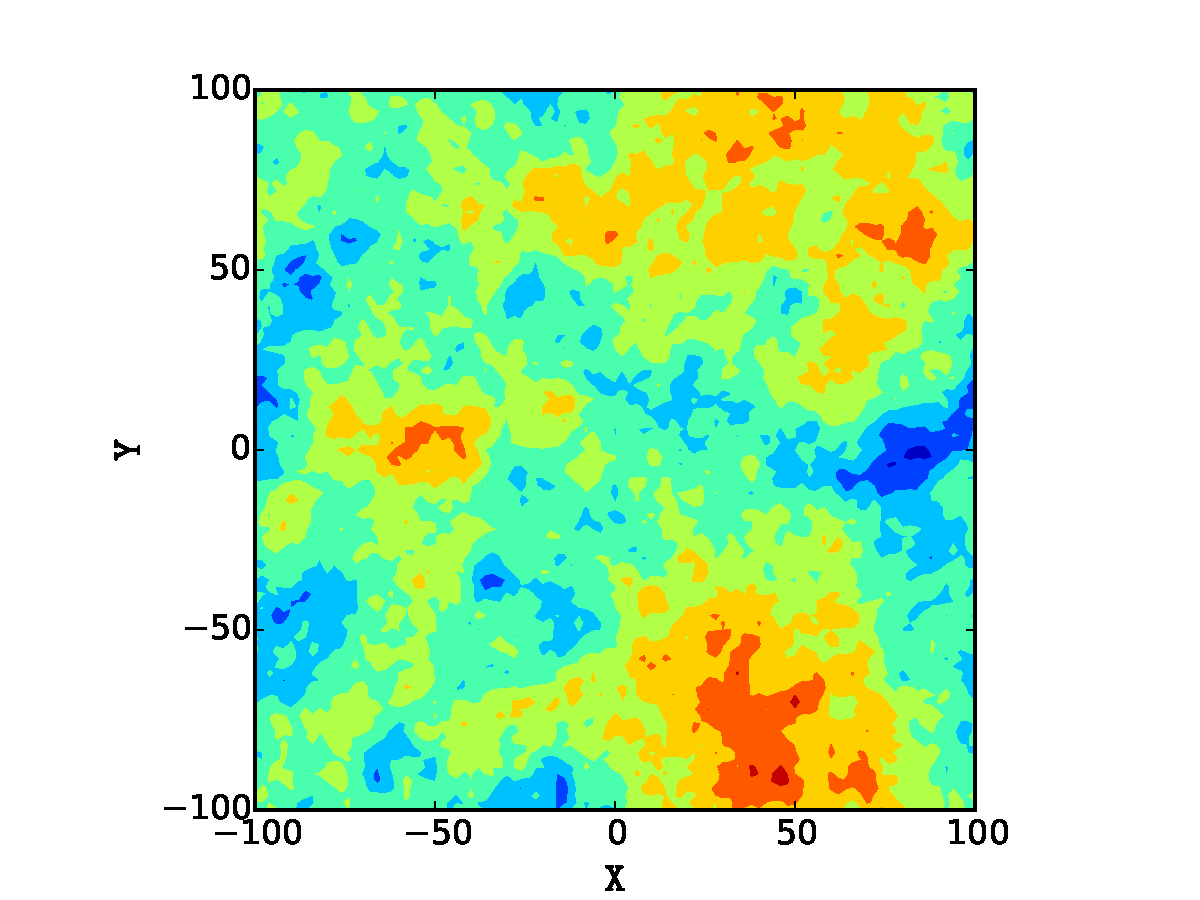
\includegraphics[width=0.32\textwidth]{figures/p5-figures/sim_grid1.pdf}
	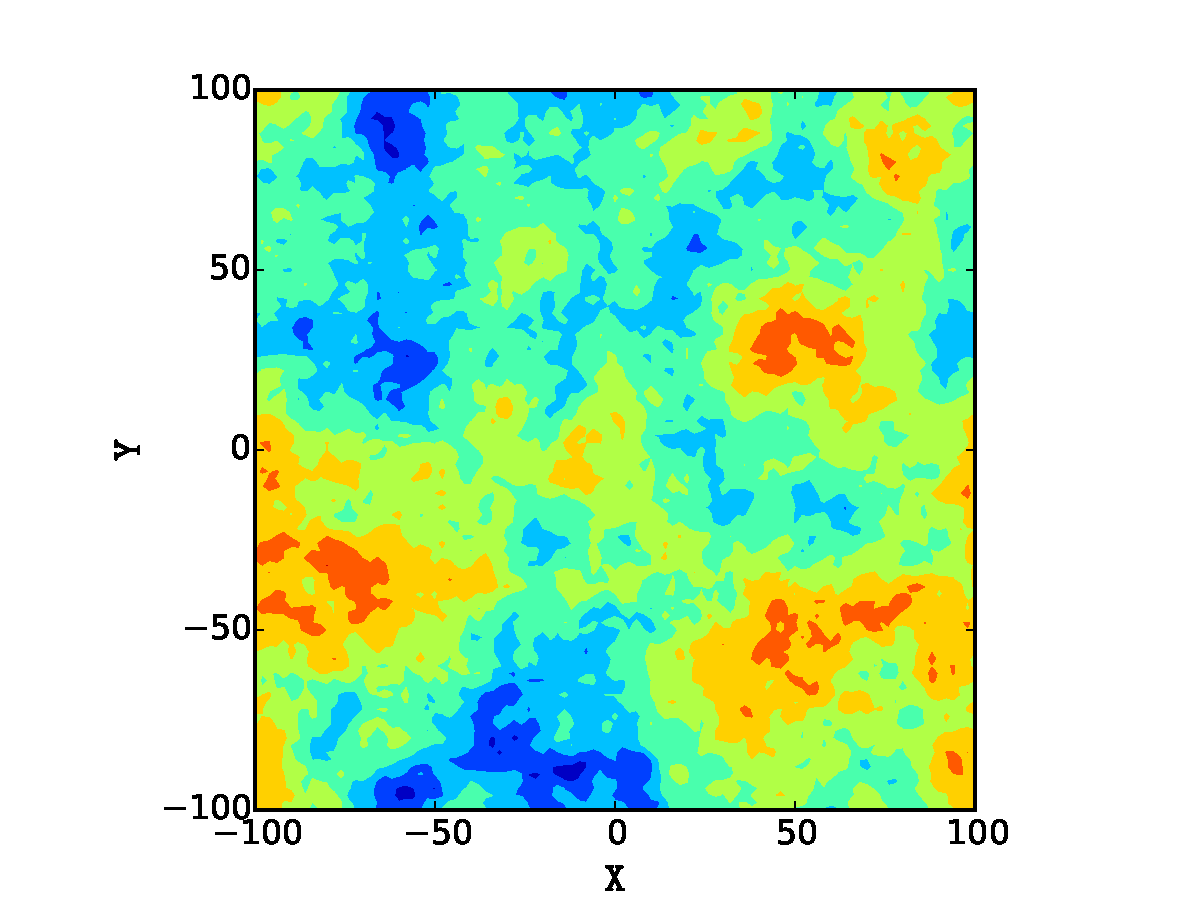
\includegraphics[width=0.32\textwidth]{figures/p5-figures/sim_grid2.pdf}
	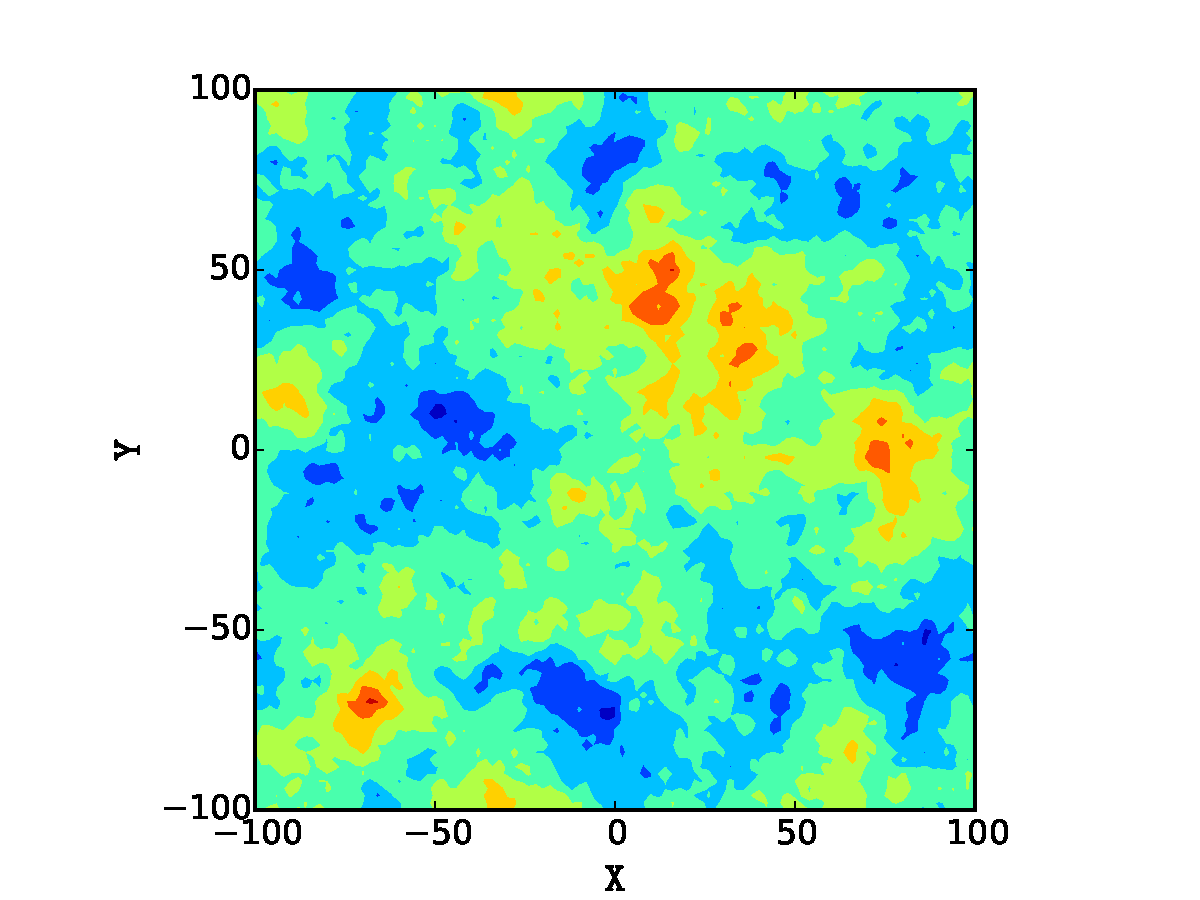
\includegraphics[width=0.32\textwidth]{figures/p5-figures/sim_grid3.pdf}\\
	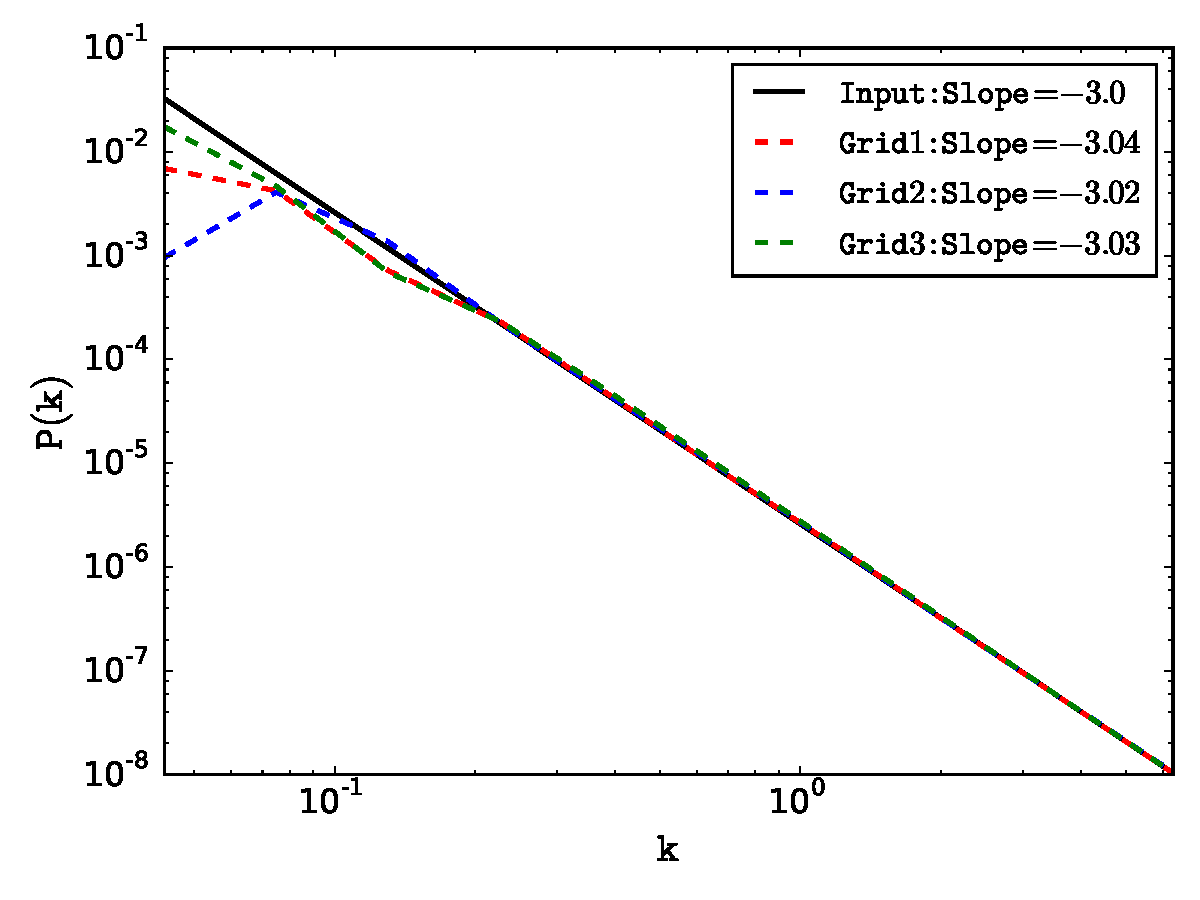
\includegraphics[width=0.48\textwidth]{figures/p5-figures/pk_simgrid_abs.pdf}
	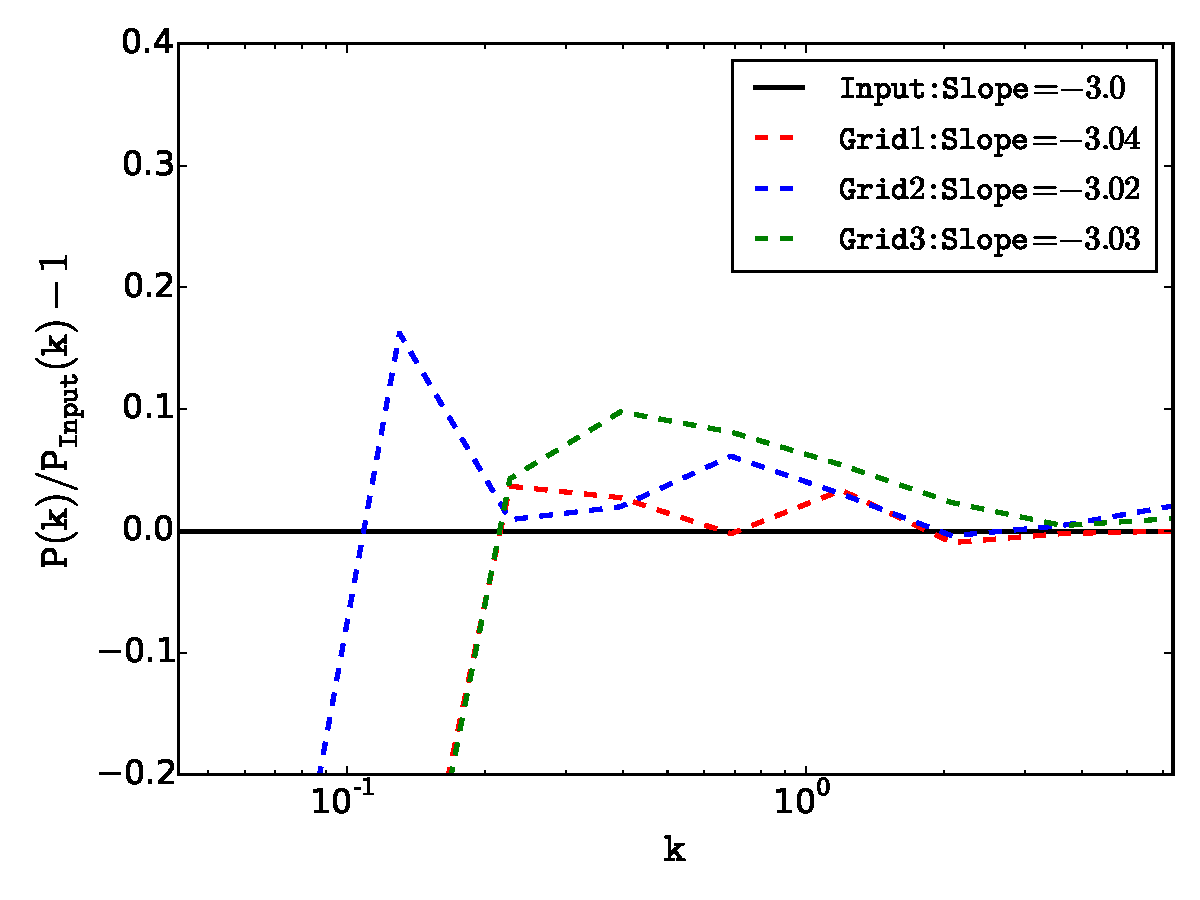
\includegraphics[width=0.48\textwidth]{figures/p5-figures/pk_simgrid.pdf}
	\caption{The first three plots (in the top row: Grid1, Grid2, Grid3) are
	the three density map realizations generated
	from the same power spectrum with $k^{-3}$ towards large $k$. The bottom-left panel shows the actual power spectra of each of the grids along with
	the true power spectrum with slope = -3.
	The bottom-right panel shows the
	comparison of the recovered power spectrum from each density grid to the input power.  These maps were only produced to test the numerical computation of the power spectrum, and have no central cluster. While it is possible to generate random fields constrained to have certain features \citep[cf.][]{1991ApJ...380L...5H} these were not needed for this simple test.}
	\label{p5:fig:simgrid}
\end{figure}

With our definition, if we have a field enclosing only one halo
with its substructures, and we compute $P_{\rm M}(k)$ at scales larger than the size of the halo, for
all those scales one gets the same mass and hence, the power above all those scales will be a constant,
which mimics the Poisson noise of the substructures in the halo model picture. Further this function
drops at scales smaller than the size of the halo,
which is the largest structure in the field, consistent
with the halo model intuition.
For a virialised halo, this function will be smooth and a power law for all scales smaller than
the size of the halo. However, if the halo is not spherically symmetric and in a merging stage
the fluctuations in the function resemble variation in its power at various scales. If one
identifies a large ensemble of halos (let's say in simulations) of nearly the same mass and
the same epoch and averages all the power spectra, one will get an unbiased trend of the clustering
properties of such halos statistically. However, studying individual systems is like studying
a random realisation of a halo which underlies a mean power spectrum and the recovered
power spectrum from such a halo should be statistically consistent with the mean.

To ensure this feature, we performed a test.  We generated three density fields which are the
random realisation of the same power spectrum ($\propto k^{-3}$ at small scales) as shown in figure
\ref{p5:fig:simgrid}. The three density grids enclose structures and some substructures and look very
different morphologically, but as they are generated from the statistics, they should show
a similar power spectrum. In the bottom-right of figure \ref{p5:fig:simgrid} we show the ratio of the
recovered power spectrum from each of the grids to the input power spectrum. The slope
of the recovered power spectrum is calculated by fitting the power law towards the larger
values of $k$, between 0.68 to 4 (in arbitrary units).
All power spectra give nearly the same slope as the input one with an error of about 10-20$\%$.
This test shows that given a density field, the correct mean statistic can be obtained within
a reasonably small error.

For a pure noise field, we expect same power at all scales. We performed this test as well (but we
don't show the result in a figure form), and verified that the power spectrum is flat.

The fluctuations in mass distribution at various scales can be directly inferred as the
presence/absence of substructures. Larger power at small scale indicates the presence of local
density peaks, however, a flat power at all scales indicates similar structures at all scales
or just the noise.  Also, a smoother distribution of the matter gives rise to smaller power whereas
sharp peaks correspond to larger power. Therefore, we expect the power at small scales to
increase as the merger progresses and reach the highest power when the system is virialised.
In other words, one should expect the power on small scales to decrease with redshift.
This form of the power spectrum can be used in order to compare halos statistically, within
simulations or observations or across the two.

%===================================================================

\section{Lens reconstruction method}\label{p5:sec:grale}

In GRALE \citep{2007MNRAS.380.1729L,2008MNRAS.389..415L} the mass
distribution is free-form and consists of a superposition of a large
number of adjustable components (several hundred Plummer lenses).  The
distribution of these Plummer lenses is adaptively determined by GRALE
using a multi-objective genetic algorithm, to optimise two fitness
measures.

\begin{enumerate}

\item The {\em overlap fitness\/} quantifies the fractional overlap of
  the projected images of the same source back onto the source plane.
  If all images of a source back-project to exactly the same area on
  the source plane, the source fitness for that image system is
  perfect.  More generally, the larger overlap the better the fitness.
  It is important to use the fractional overlap, as otherwise the
  fitness measure would be biased towards extreme magnifications.

\item The {\em null fitness\/} is a penalty for any spurious images
  implied by a model where none are present in the observations.
  A null space is created at the image plane, subdivided into a number of
  triangles, and the trial solution
  under study is used to project these triangles onto the source plane. Then, the
  amount of overlap between each triangle and the current estimate of the source
  shape is calculated and used to construct a null space fitness measure which
  is the penalty. The
  penalty is applied only in regions where the data make it clear that
  no images are present; extra images are allowed in regions that are
  difficult to observe because, for example, of the presence of nearby
  bright galaxies.  Among lens-modelling techniques, GRALE is unique
  in being able to exploit the {\em absence\/} of images as useful
  information.

\end{enumerate}

Further fitness measures can be defined and incorporated into GRALE,
in particular, time delays
\citep{2009MNRAS.397..341L,2015PASJ...67...21M}.  No information about
the light from the cluster is used --- mass-traces-light assumptions
are completely absent.

While the genetic algorithm optimizes the properties and placement of
the component Plummer lenses, the user still needs to specify a range
for the allowed number of components.  This is, in effect, an overall
resolution of the mass map.  To set this effective resolution, we run
the mass reconstruction process first at coarse resolution, then
finer, and then coarse again, and choose an optimal trade-off between
fitness and resolution --- see \cite{2014MNRAS.439.2651M} for details
and tests of this strategy.  Finally, the entire cycle is repeated 30
times (while using pre-HFF data) or 40 times (while using post-HFF data),
to generate an ensemble of mass reconstructions. In the remainder
of the article, we present the average mass map of 30 (or 40) mass reconstructions
for each cluster lens, unless stated otherwise. The power spectra
for each of the reconstructions were computed, and both average power spectra
as well as the power spectra of the average mass map are presented. For the true
error estimates, the former is more useful.

%==========================================================================

\section{Hubble Frontier Fields}\label{p5:sec:hff}

Hubble Frontier Fields (HFF) survey (PI: J.Lotz, HST 13498) is a three year
Director's Discretionary Time program that devotes a total of 840 orbits to six
galaxy clusters plus the accompanying parallel fields.  Each field is observed in
three HST optical bands (ACS F435W, F606W and F814W) and four infra-red bands (WFC3-IR
F105W, F125W, F140W, and F160W).
It is the single most ambitious commitment of HST resources to the exploration of
the distant Universe through the power of gravitational lensing by massive galaxy
clusters. All six clusters are early or intermediate stage mergers at $z=0.3$--0.55,
with significant elongation and hence a non-trivial mass distribution. Each had about
10--20 multiply imaged background sources discovered with pre-HFF HST
data. Five independent teams were tasked with making mass and magnification maps for
these six clusters. In the analysis of the present paper, we use mass maps presented
by our team, made with pre-HFF lensing data on six clusters as well as two maps made
with post-HFF data, for clusters MACS0416 and Abell 2744. Table \ref{p5:tbl:HFF} shows the necessary
information about the lensing data in each of the HFF clusters.
In the following figures, the mass maps and the corresponding power spectra are
marked as $\mathtt{v1}$ and $\mathtt{v3}$ indicating pre-HFF and post-HFF data respectively.

\begin{table}
\centering
\resizebox{\textwidth}{!}{%
\begin{tabular}{ l | l | c | c | c | c  }
  \hline
  Cluster & Data & Redshift & Number of images & Number of sources & Redshift range of sources \\
  \hline
  MACS-J0416 & pre-HFF & 0.396 & 40 & 13 & 1.82-3.25 \\
  MACS-J0416 & post-HFF & 0.396 & 88 & 36 & 1.00-5.90 \\
  Abell 2744 & pre-HFF & 0.308 & 41 & 12 & 2.00-4.00 \\
  Abell 2744 & post-HFF & 0.308 & 55 & 18 & 2.00-4.00 \\
  Abell 370 & pre-HFF & 0.375 & 36 & 11 & 0.73-3.00 \\
  AS-1063 & pre-HFF & 0.348 & 37 & 13 & 1.22-6.09 \\
  MACS-1149 & pre-HFF & 0.543 & 32 & 11 & 1.23-3.80 \\
  MACS-0717 & pre-HFF & 0.545 &  23 & 7 & 1.80-2.91 \\
  \hline
\end{tabular}%
}
\caption{Lensing data from different HFF clusters.}
\label{p5:tbl:HFF}
\end{table}


%------------------------------------------------
\subsection{MACS J0416.1-2403}\label{p5:sec:0416}
\begin{figure}
	\centering
	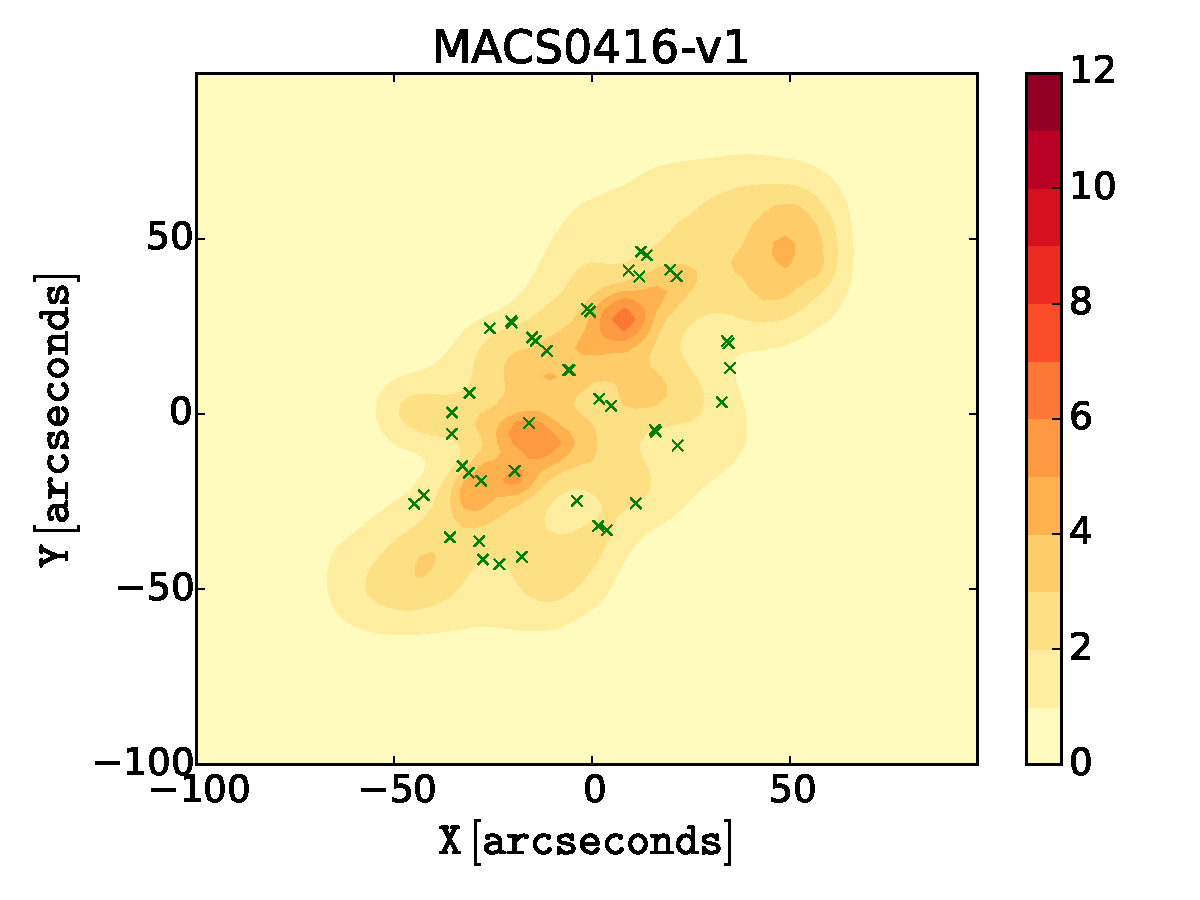
\includegraphics[width=0.48\textwidth]{figures/p5-figures/MACS0416-1_SL.pdf}
	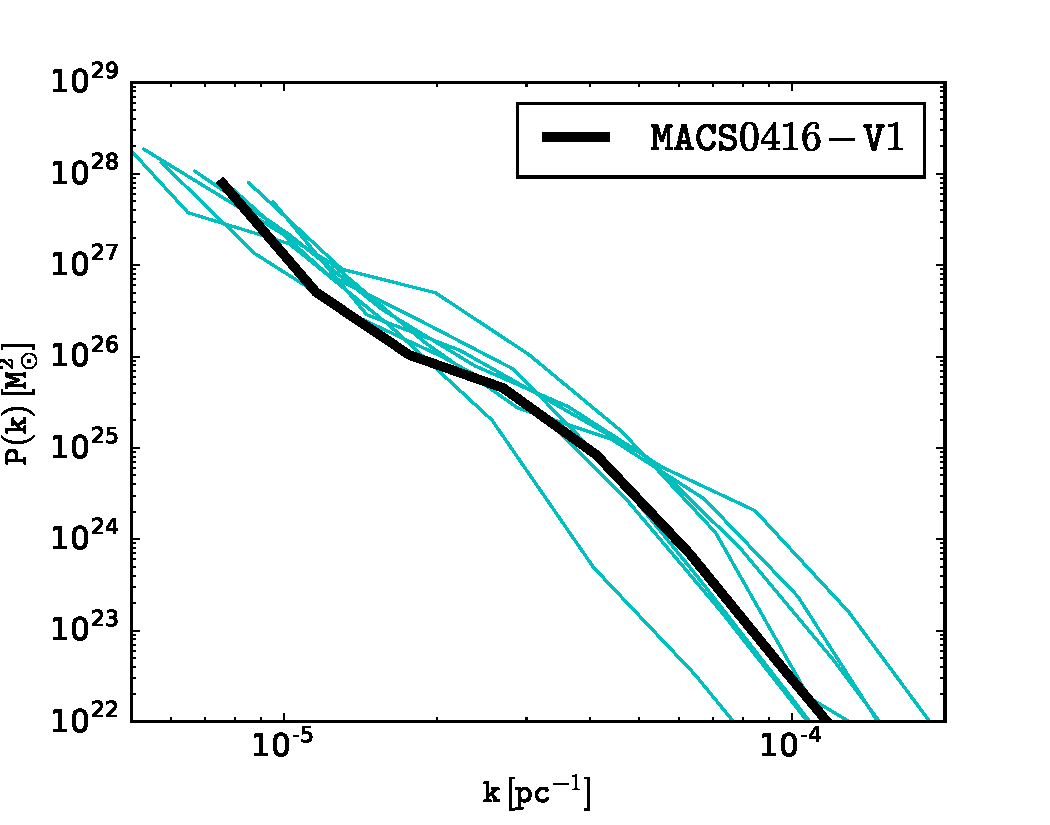
\includegraphics[width=0.48\textwidth]{figures/p5-figures/pk_MACS0416-V1.pdf}\\
	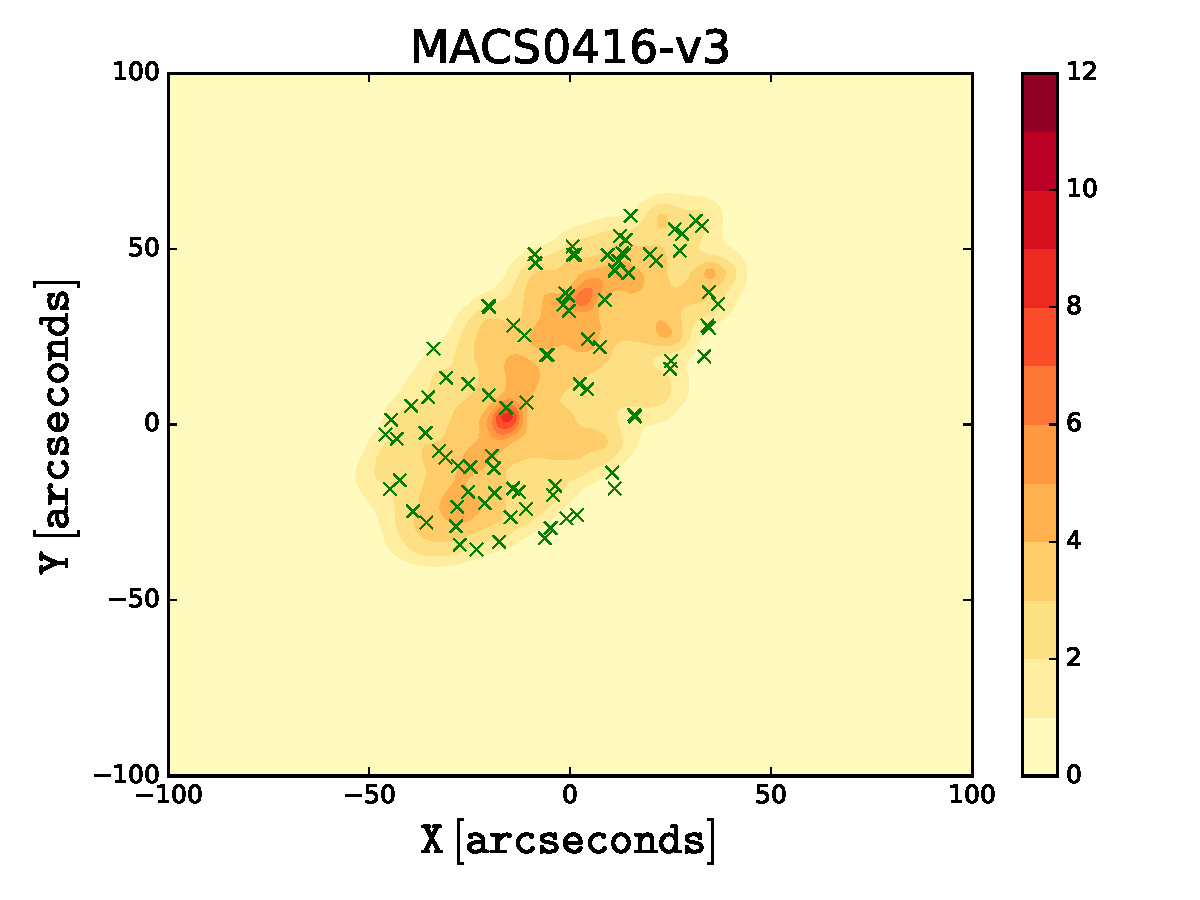
\includegraphics[width=0.48\textwidth]{figures/p5-figures/MACS0416-3_SL.pdf}
	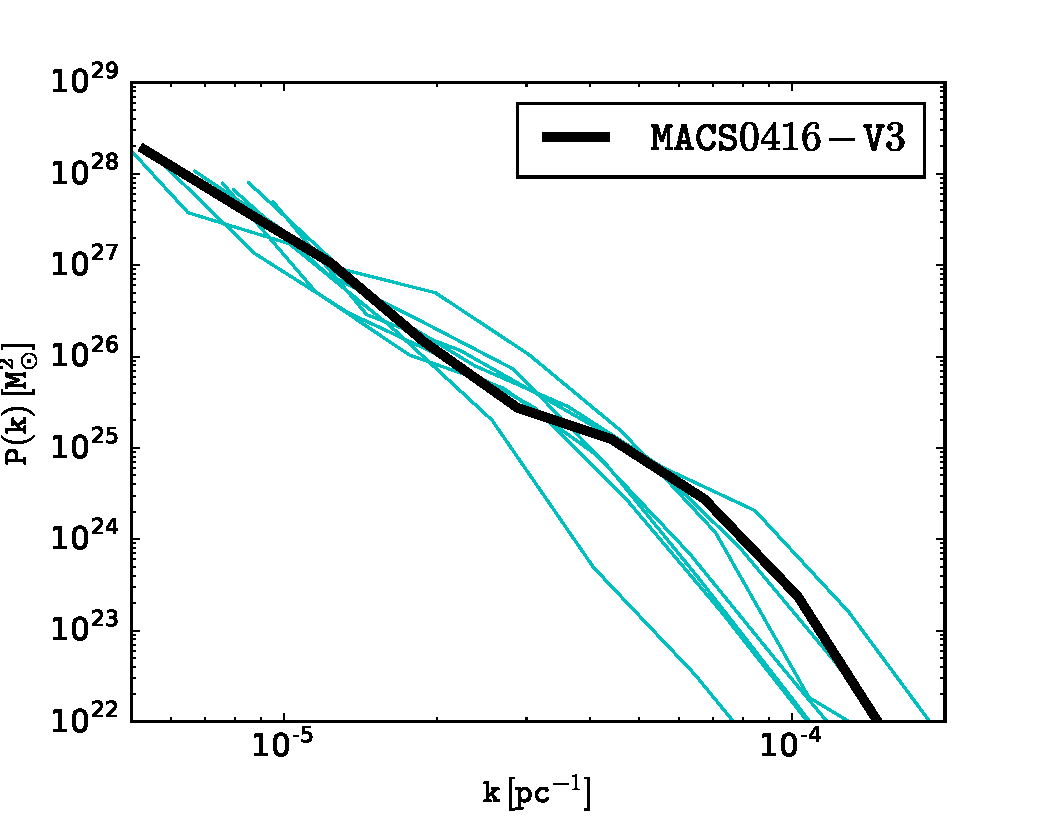
\includegraphics[width=0.48\textwidth]{figures/p5-figures/pk_MACS0416-V3.pdf}
	\caption{Left: the density map for MACS0416 cluster using pre-HFF
	data (top row) and HFF data (bottom row). The crosses mark the positions
	of the lensed images.
	Right: the highlighted (black)
	corresponding power spectrum of the cluster on the left with all other
	HFF clusters' power spectra in the background.}
	\label{p5:fig:density:0416}
\end{figure}



MACS J0416.1-2403 (MACS0416 henceforth) is a strong gravitational lens at redshift of
nearly 0.396. It is an elongated galaxy cluster, most probably a recent merger or a pre-merger
\citep{ogr15}, and hence has a non-trivial mass distribution. It was first identified by the MAssive
Cluster Survey \citep[MACS;][]{2010MNRAS.407...83E}. Based on its double-
peaked surface brightness in the X-rays \citep{2012MNRAS.420.2120M},
its recent merger stage is confirmed. It is amongst the five high magnification
clusters in the CLASH (Cluster Lensing and Supernovae survey with Hubble) project
\citep{2012ApJS..199...25P}. Detailed mass maps were provided by
\cite{2013ApJ...762L..30Z} using CLASH data, and \cite{2015MNRAS.446.4132J}
and \cite{2015arXiv150708960S} using HFF data.

We made two reconstructions of this lens using GRALE, one with pre-HFF data (total
40 images from 13 sources), using data from \cite{2011MNRAS.417..333M}, as well as data provided by
J. Richard and D. Coe, and one with HFF data (total 88 images from 36 sources) 
where we used images that were classified collectively by the HFF teams
being of GOLD and SILVER quality. Many of these images were initially identified by
\cite{2015MNRAS.446.4132J}. The two reconstructed mass models, $\mathtt{v1}$ and
$\mathtt{v3}$---with each being an average
of 30 and 40 realisations respectively---are shown in figure \ref{p5:fig:density:0416} (left column),
each with its respective power spectrum (highlighted in the right column). Both mass models
are very similar at large scales, which is also evident from the power spectrum, and
only differ in the details at small scales. The two mass clumps and the elongation
can be identified in both models. However, the mass models with HFF data (bottom row),
shows larger power or many detailed substructures at small scales. This is
expected as HFF data has many more lensed images than pre-HFF data and hence provides additional
lensing constraints at small scales, which leads to increased power at larger $k$'s.

%------------------------------------------------
\subsection{Abell 2744}\label{p5:sec:2744}
\begin{figure}
	\centering
	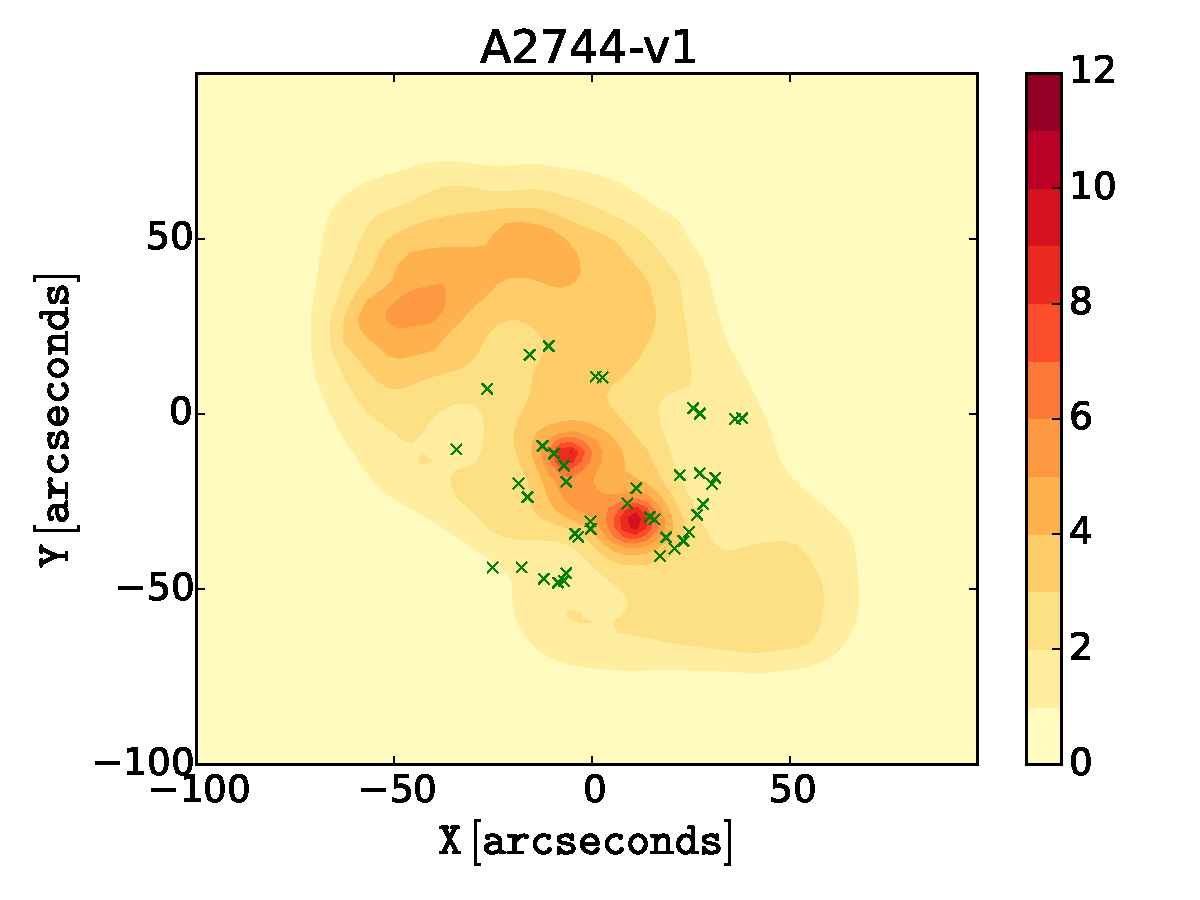
\includegraphics[width=0.48\textwidth]{figures/p5-figures/A2744_SL.pdf}
	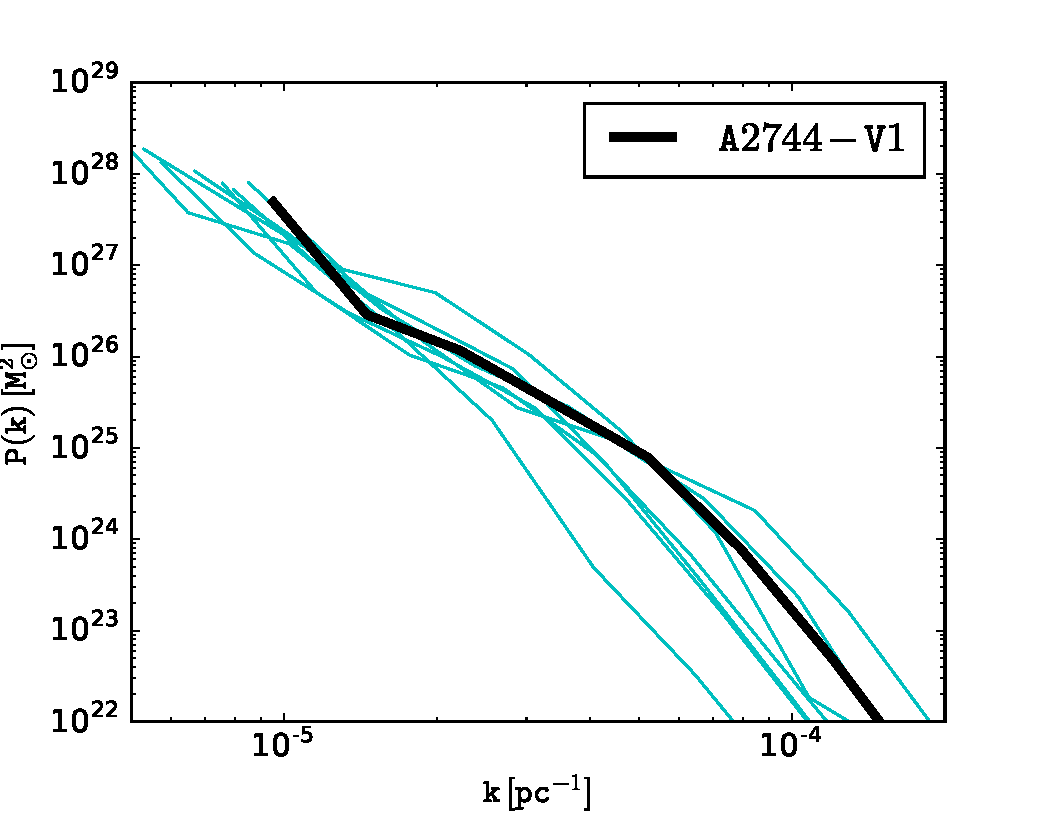
\includegraphics[width=0.48\textwidth]{figures/p5-figures/pk_A2744-V1.pdf}
  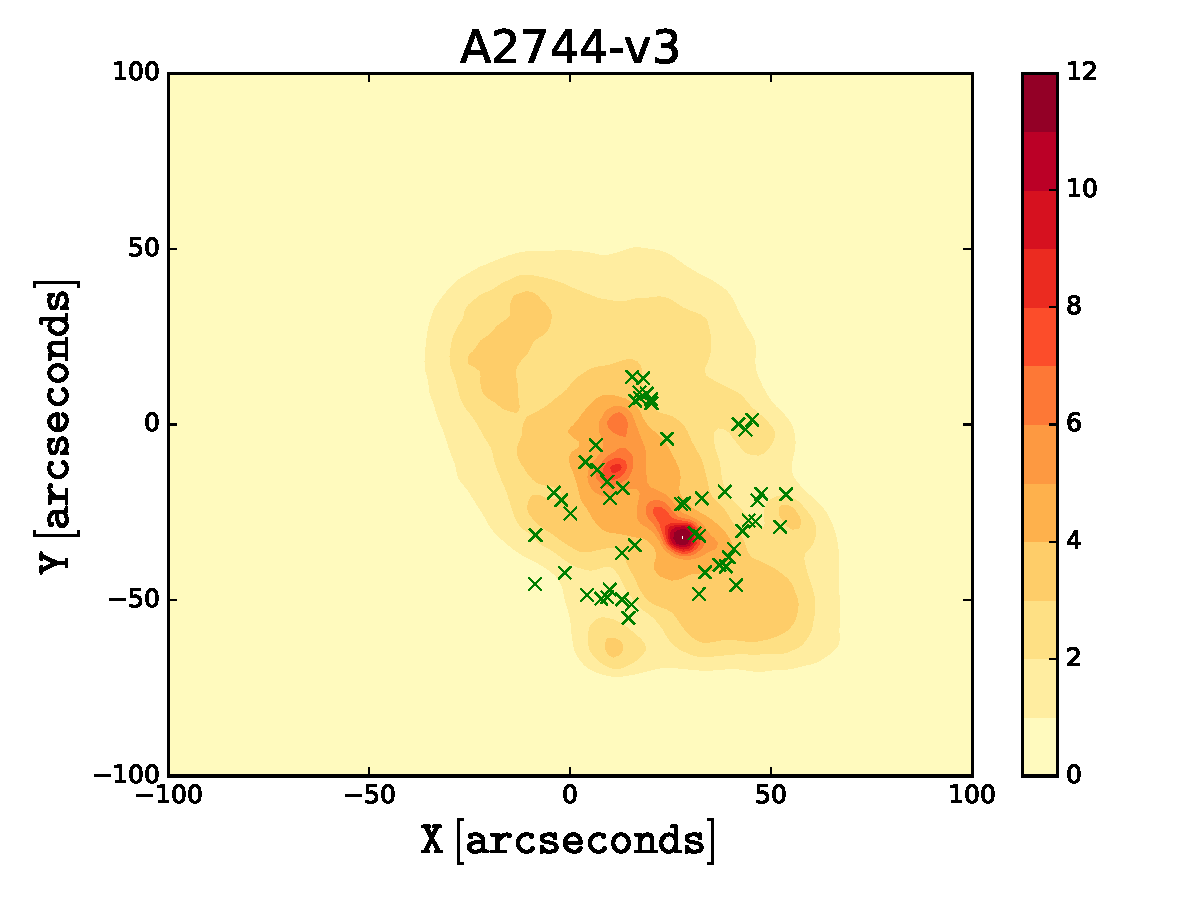
\includegraphics[width=0.48\textwidth]{figures/p5-figures/A2744-3_SL.pdf}
  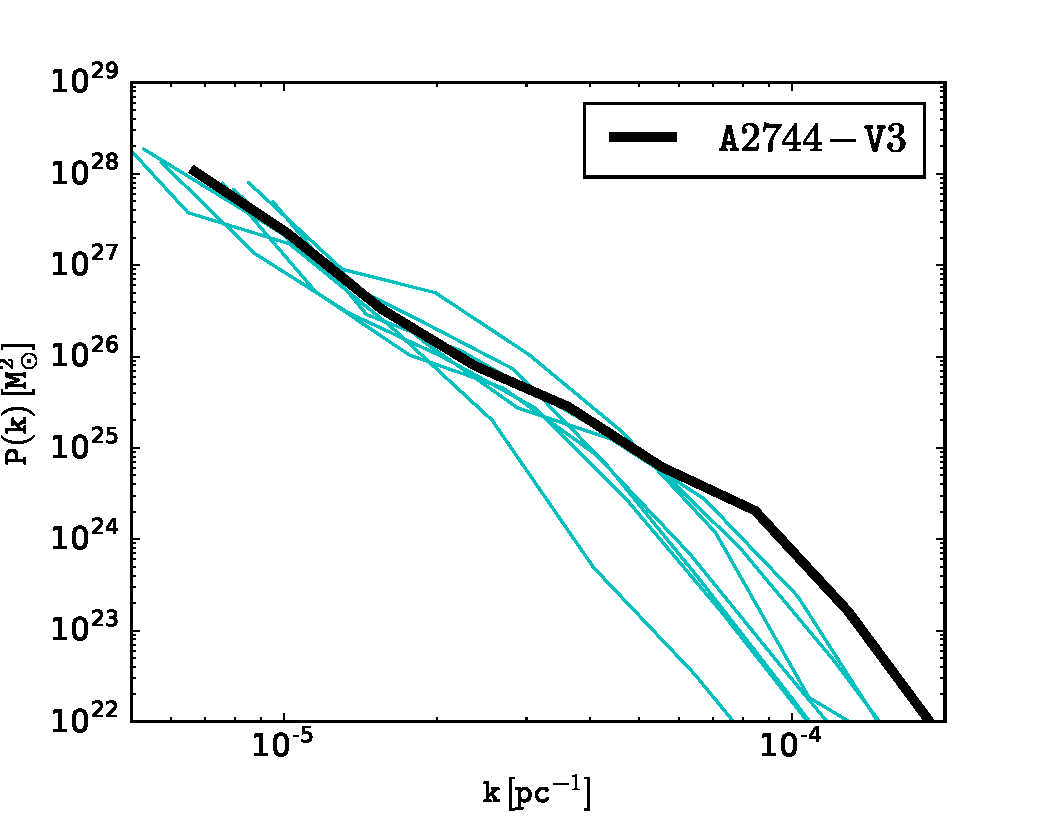
\includegraphics[width=0.48\textwidth]{figures/p5-figures/pk_A2744-V3.pdf}
	\caption{Left: the density map for the Abell 2744 cluster using
	 pre-HFF data (top row) and post-HFF data (bottom row). 
   The upper left clump could well be an
	 artefact as there
	 are no images there.
	 Right: the highlighted (black) corresponding power
	 spectrum of the cluster on the left with all other
	HFF clusters' power spectra in the background.}
	\label{p5:fig:density:2744}
\end{figure}

Abell 2744 is a massive galaxy cluster at redshift 0.308 and an active merger.
It has been studied in various wavelengths, for example, it has an extended radio halo
\citep{1999NewA....4..141G,2001A&A...369..441G}, X-ray emission
\citep{1998MNRAS.296..392A,2010MNRAS.407...83E,2004MNRAS.349..385K,2011ApJ...728...27O}
and various substructures have been identified in the optical observations
\citep{2001ApJ...548...79G,2006A&A...449..461B}.
\cite{2010MNRAS.406.1134S} show a significant offset between the dark-matter
component (from lensing) and baryonic matter (from X-rays observations).
There is also a magnified singly imaged supernova in the background,
at redshift 1.35 \citep{rod15}.
Various lensing analyses have been done
\citep{1997ApJ...479...70S,1998MNRAS.296..392A,2004ApJ...613...95C,
2011MNRAS.417..333M,2014ApJ...797...98L,2014arXiv1409.8663J}.

We present two mass models of Abell 2744 using GRALE, one with pre-HFF data
\citep{2011MNRAS.417..333M,2014MNRAS.444..268R} as well as data provided by J. Richard and D. Coe, for
 a total of 41 images from 12 background sources spread over a redshift range of 2 to 4 and
 another with post-HFF data for a total of 55 images from 18 sources. Figure
\ref{p5:fig:density:2744} shows the reconstructed mass maps and the corresponding
power spectra. It shows two very distinct blobs and an overall
elongated structure, a morphology very likely for a major merger which is in fact confirmed
by previous studies. The post-HFF data contains improved identifications and positions
of the lensing images, and the corresponding map (bottom row of figure \ref{p5:fig:density:2744}) shows fewer spurious structures compared to the pre-HFF map (top row of figure \ref{p5:fig:density:2744}). 

Due to very sharp mass peaks, this cluster, like MACS0416, also shows larger power at small scales.



%------------------------------------------------
\subsection{Abell 370}\label{p5:sec:370}
\begin{figure}
	\centering
	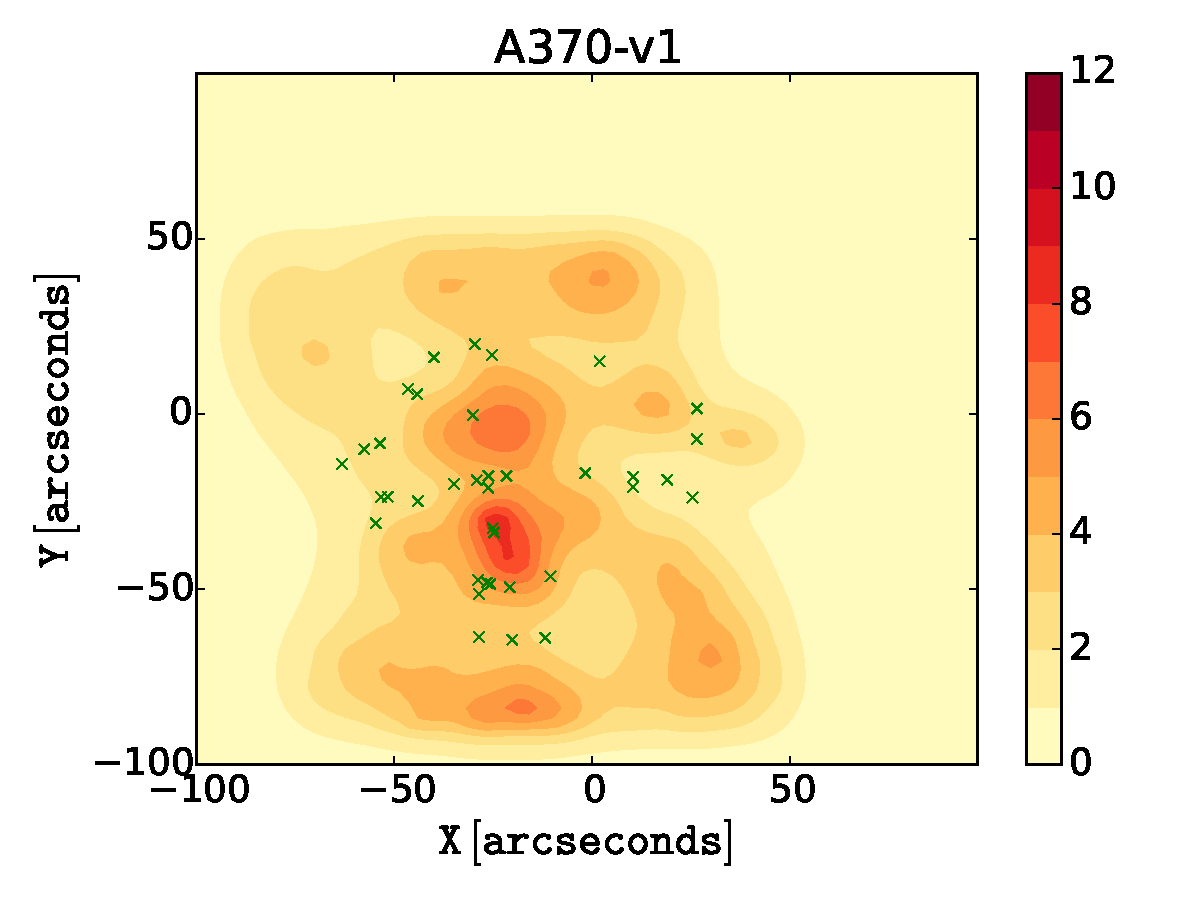
\includegraphics[width=0.48\textwidth]{figures/p5-figures/A370_SL.pdf}
	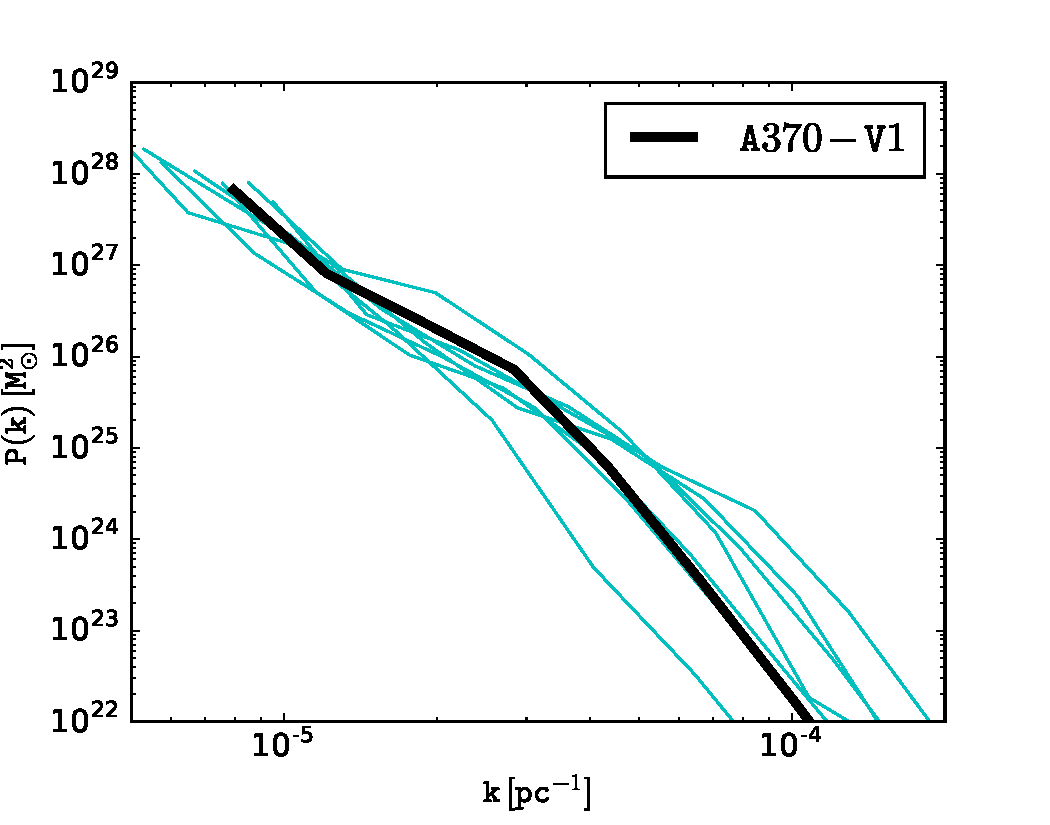
\includegraphics[width=0.48\textwidth]{figures/p5-figures/pk_A370-V1.pdf}
	\caption{Left: the density map for the Abell 370 cluster using
	 pre-HFF data. Right: the highlighted (black) corresponding power
	 spectrum of the cluster on the left with all other
	HFF clusters' power spectra in the background.}
	\label{p5:fig:density:370}
\end{figure}


Abell 370 is a strong gravitational lens at redshift 0.375 and hosts a giant
gravitational arc at redshift 0.725. Due to its large Einstein radius, it is
an ideal target to look for high redshift galaxies through its magnification, especially
in high-density regions. There are many published mass models
\citep[for example][]{1987Msngr..50....5S,1998MNRAS.294..734A,ric10}.
We used pre-HFF data from the latter work, as well as data provided by D. Coe and A. Koekemoer,
to reconstruct its mass distribution. Figure \ref{p5:fig:density:370}
shows the resulting mass map. The mass distribution is shallow but shows many
substructures. The resulting power spectrum shows less power on small scales
as compared to other HFF clusters which is reflected in shallower peaks in
its mass distribution.


%------------------------------------------------
\subsection{Abell S1063}\label{p5:sec:1063}
\begin{figure}
	\centering
	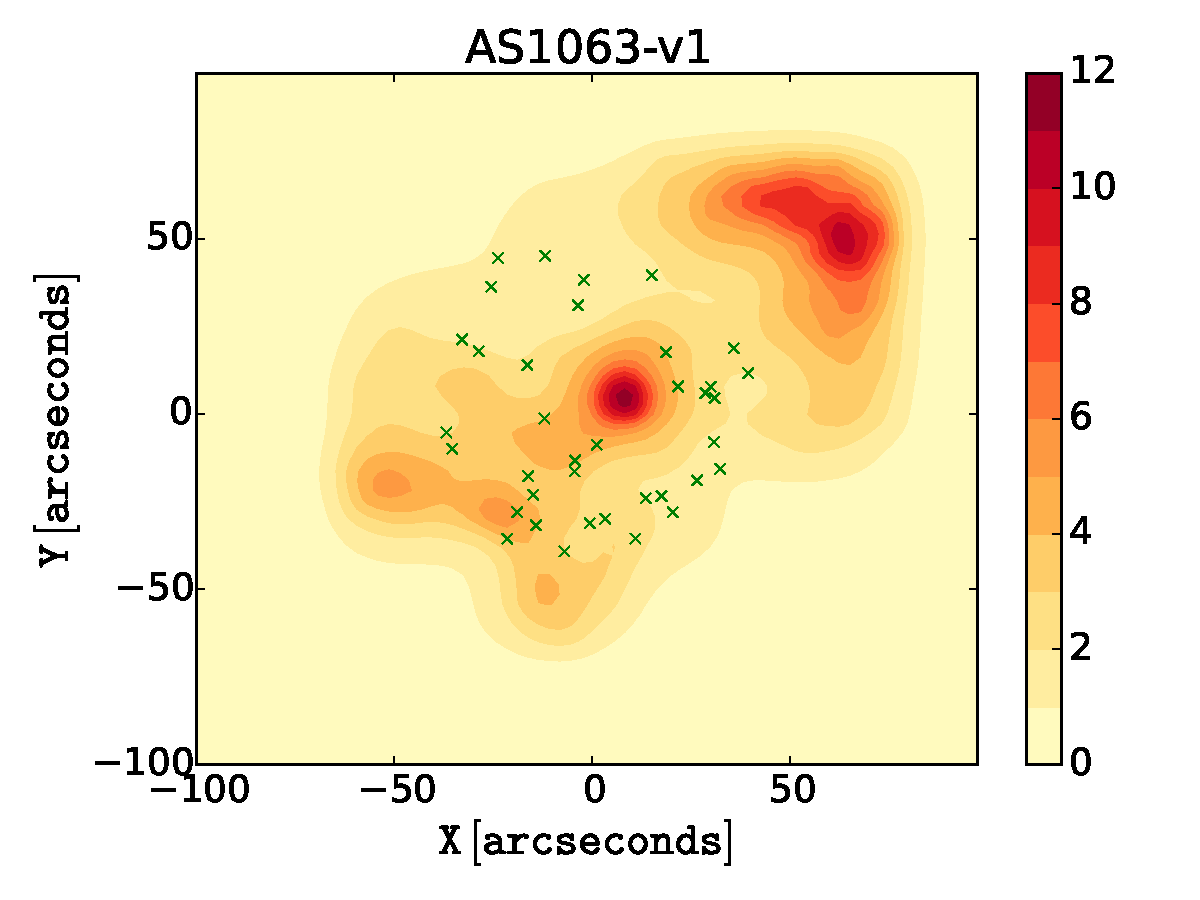
\includegraphics[width=0.48\textwidth]{figures/p5-figures/AS1063_SL.pdf}
	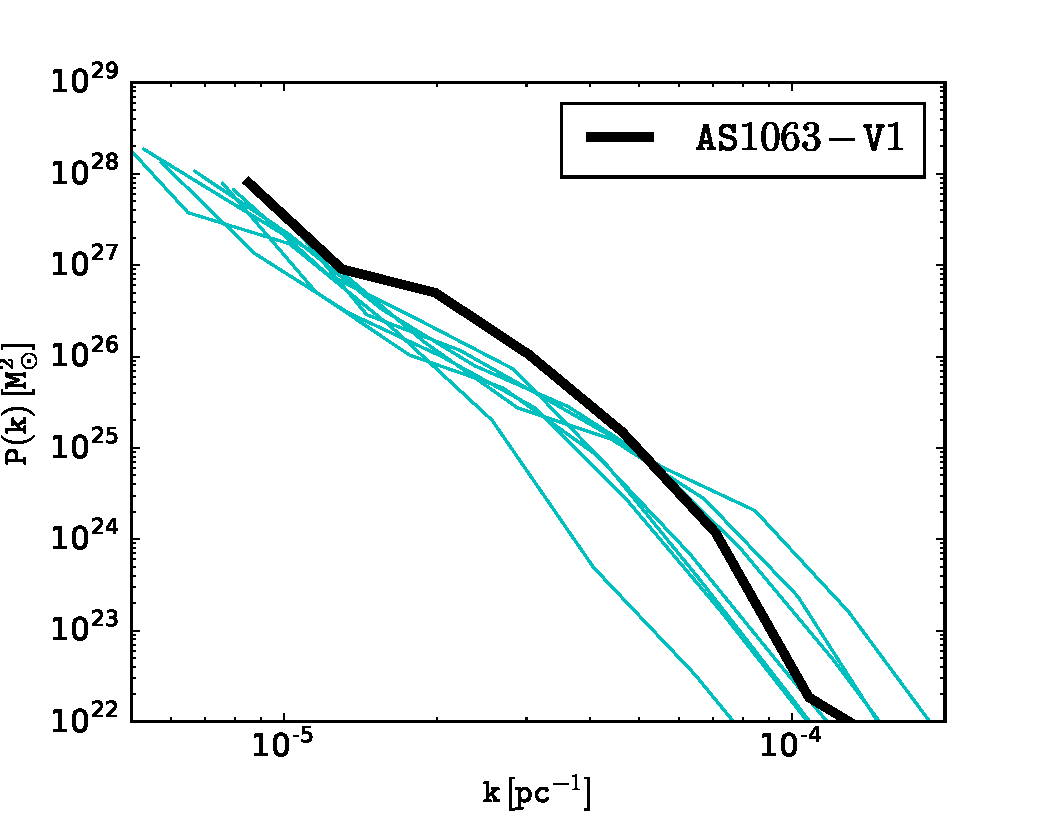
\includegraphics[width=0.48\textwidth]{figures/p5-figures/pk_AS1063-V1.pdf}
	\caption{Left: the density map for the AS1063 cluster using
	 pre-HFF data. Right: the highlighted (black) corresponding power
	 spectrum of the cluster on the left with all other
	HFF clusters' power spectra in the background.
	Note that there are no images in the upper right corner of the map, so the massive
	clump in that region could well be an artefact.
	}
	\label{p5:fig:density:1063}
\end{figure}

Abell S1063 is a galaxy cluster at redshift 0.348. We used pre-HFF data identified
by \cite{2014MNRAS.444..268R}; our reconstruction used a total of 37 images from 13 background
sources.

Figure \ref{p5:fig:density:1063} shows the reconstructed mass map along with the
corresponding power spectrum. It shows two mass clumps, which lead to
larger power at intermediate scales, but due to the shallowness of the peaks, it loses
power at small scales.



%------------------------------------------------
\subsection{MACS J1149.5+2223}\label{p5:sec:1149}
\begin{figure}
	\centering
	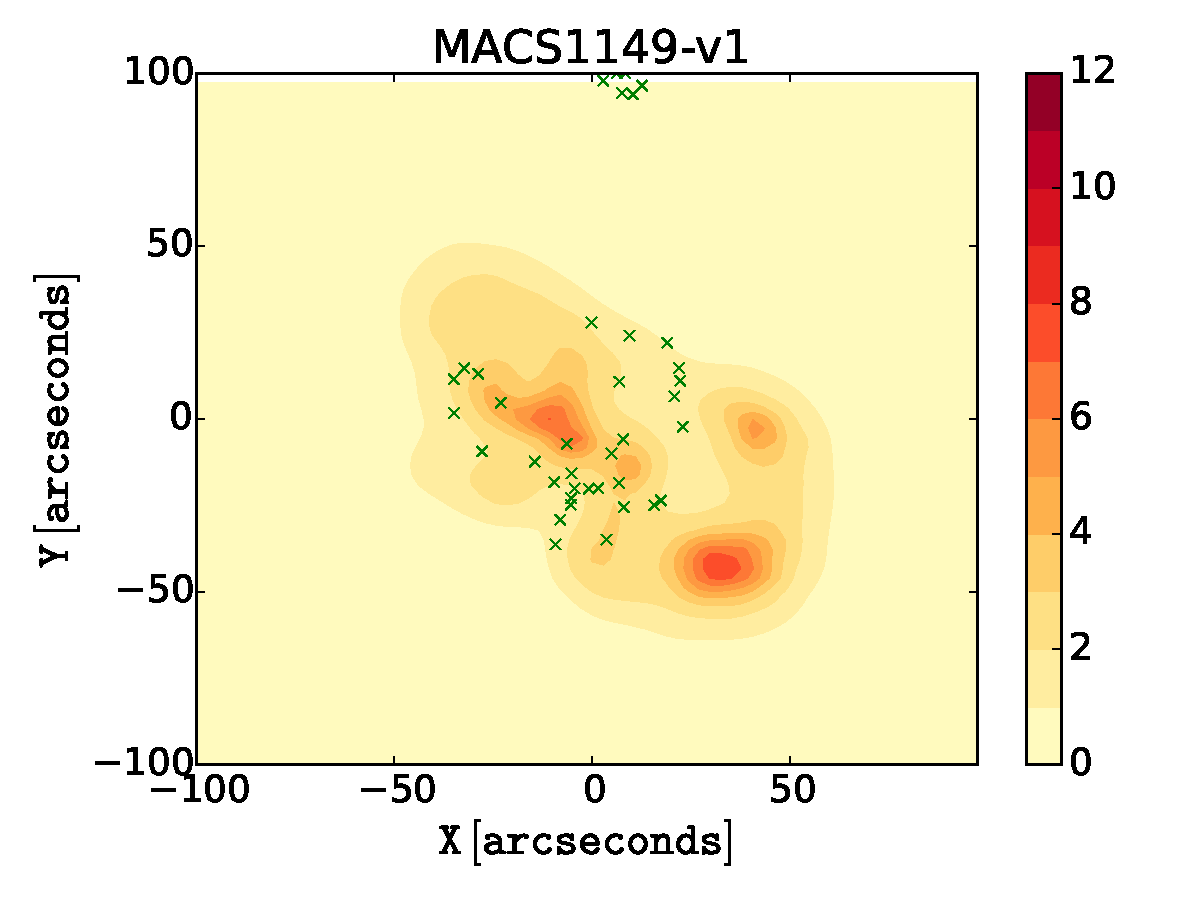
\includegraphics[width=0.48\textwidth]{figures/p5-figures/MACS1149_SL.pdf}
	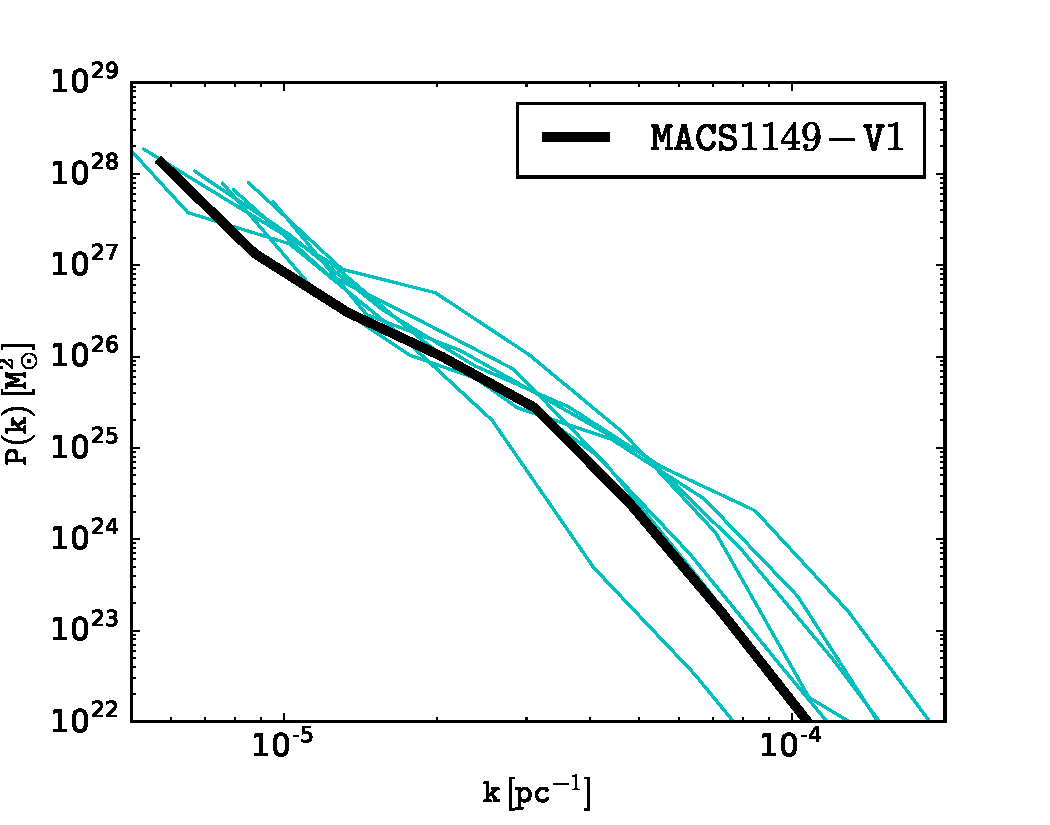
\includegraphics[width=0.48\textwidth]{figures/p5-figures/pk_MACS1149-V1.pdf}
	\caption{Left: the density map for the MACS1149 cluster using
	 pre-HFF data. Right: the highlighted (black) corresponding power
	 spectrum of the cluster on the left with all other
	HFF clusters' power spectra in the background.
There are no images beyond X=25'', so the two clumps on the right
could well be artefacts.
        }
	\label{p5:fig:density:1149}
\end{figure}

MACS J1149+2223 (MACS1149 hereafter) is an X-ray bright cluster at redshift 0.543.
It has been studied by various authors for its rich strong lensing
\citep{2009ApJ...707L.163S,2009ApJ...703L.132Z,2011MNRAS.410.1939Z,2015ApJ...801...44Z,2014MNRAS.443..957R,2014ApJ...797...48J,2015ApJ...800L..26S}.
There is also a multiply imaged supernova
\citep{2014ATel.6729....1K,2015Sci...347.1123K} hosted by a face-on spiral galaxy
at redshift 1.49.

Figure \ref{p5:fig:density:1149} shows the reconstructed mass model of MACS1149 using
GRALE with pre-HFF data (total 32 images from 11 background sources) from
\cite{2009ApJ...707L.163S,2009ApJ...703L.132Z}, and data provided by M. Limousin.
The mass
model favours two dominant peaks and one sub-peak, elongation and many substructures.
The peaks are shallower than those in Abell 2744, also expected as it has nearly the
same mass as Abell 2744 but higher redshift. The corresponding power spectrum is shown
in the right column of the same figure.



%------------------------------------------------


\subsection{MACS J0717.5+3745}\label{p5:sec:0717}
\begin{figure}
	\centering
	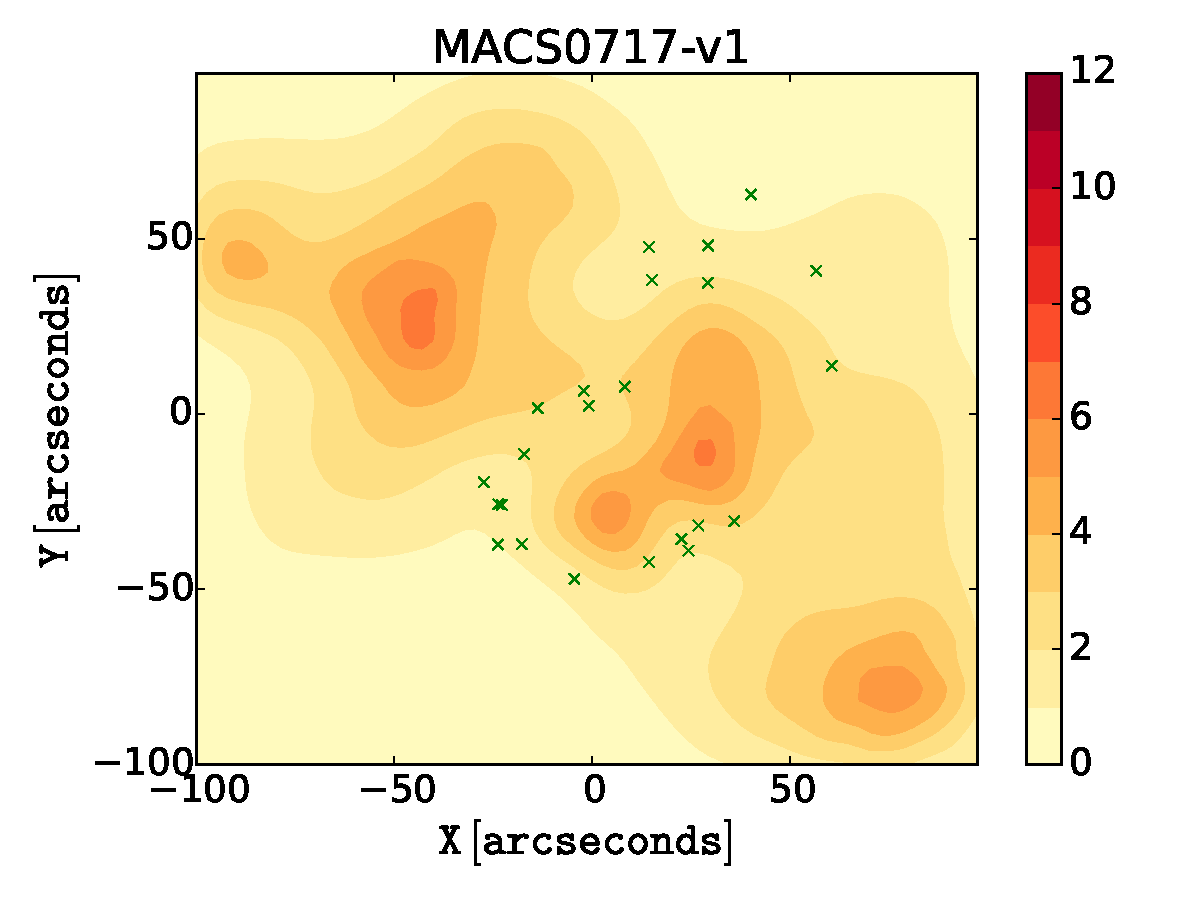
\includegraphics[width=0.48\textwidth]{figures/p5-figures/MACS0717_SL.pdf}
	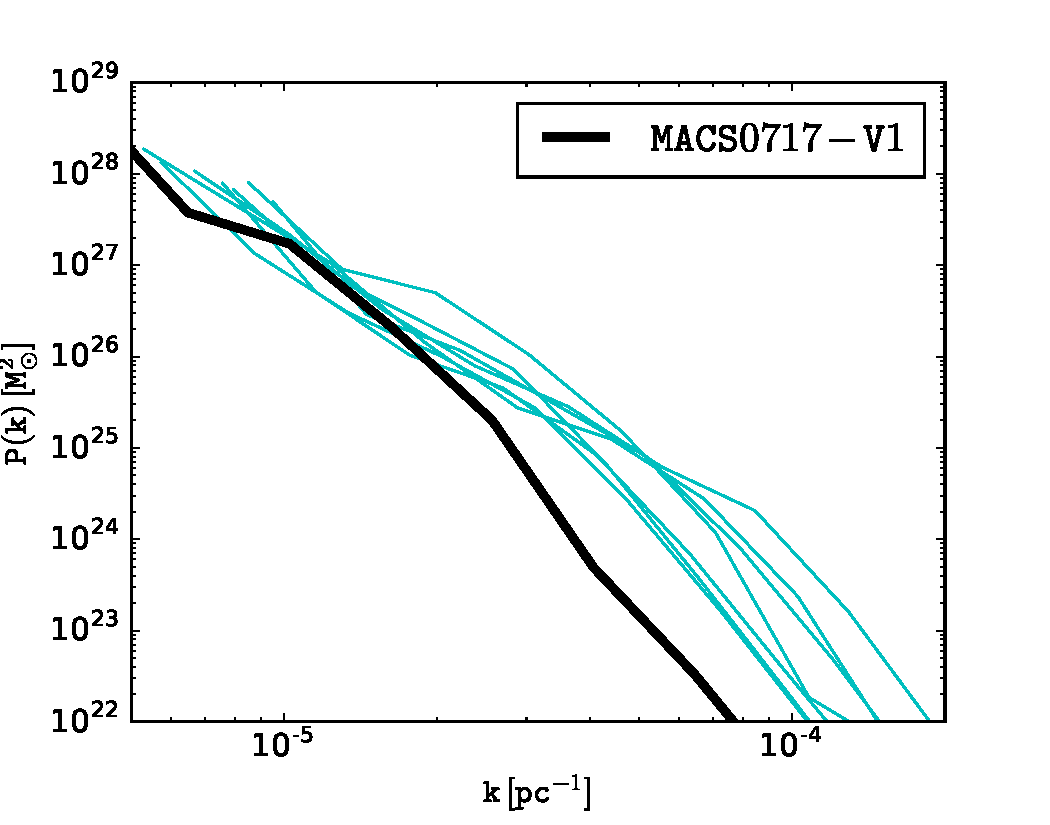
\includegraphics[width=0.48\textwidth]{figures/p5-figures/pk_MACS0717-V1.pdf}
	\caption{Left: the density map for the MACS0717 cluster using
	 pre-HFF data. The upper left and bottom right clumps could
	 well be artefacts as there
	 are no images there.
	 Right: the highlighted (black) corresponding power
	 spectrum of the cluster on the left with all other
	HFF clusters' power spectra in the background.}
	\label{p5:fig:density:0717}
\end{figure}


MACS J0717.5+3745 (MACS0717 hereafter) is a strong gravitational lens at redshift 0.55,
classified as the most dramatic merger in X-ray/optical analysis by
\cite{2012MNRAS.420.2120M}.

We used pre-HFF data from \cite{2012A&A...544A..71L,2014MNRAS.444..268R} and \cite{med13} to reconstruct
its mass distribution using GRALE. Figure \ref{p5:fig:density:0717} shows the resulting
mass map and the corresponding power spectrum. Due to the clear mass peaks and substructures,
the power spectrum shows increased power at intermediate scales, however, due to very shallow peaks the
power spectrum at small scales drops and is amongst the lowest of the HFF clusters.


%------------------------------------------------

\section{Comparing the clusters}\label{p5:sec:comparison}


\begin{figure}
	\centering
  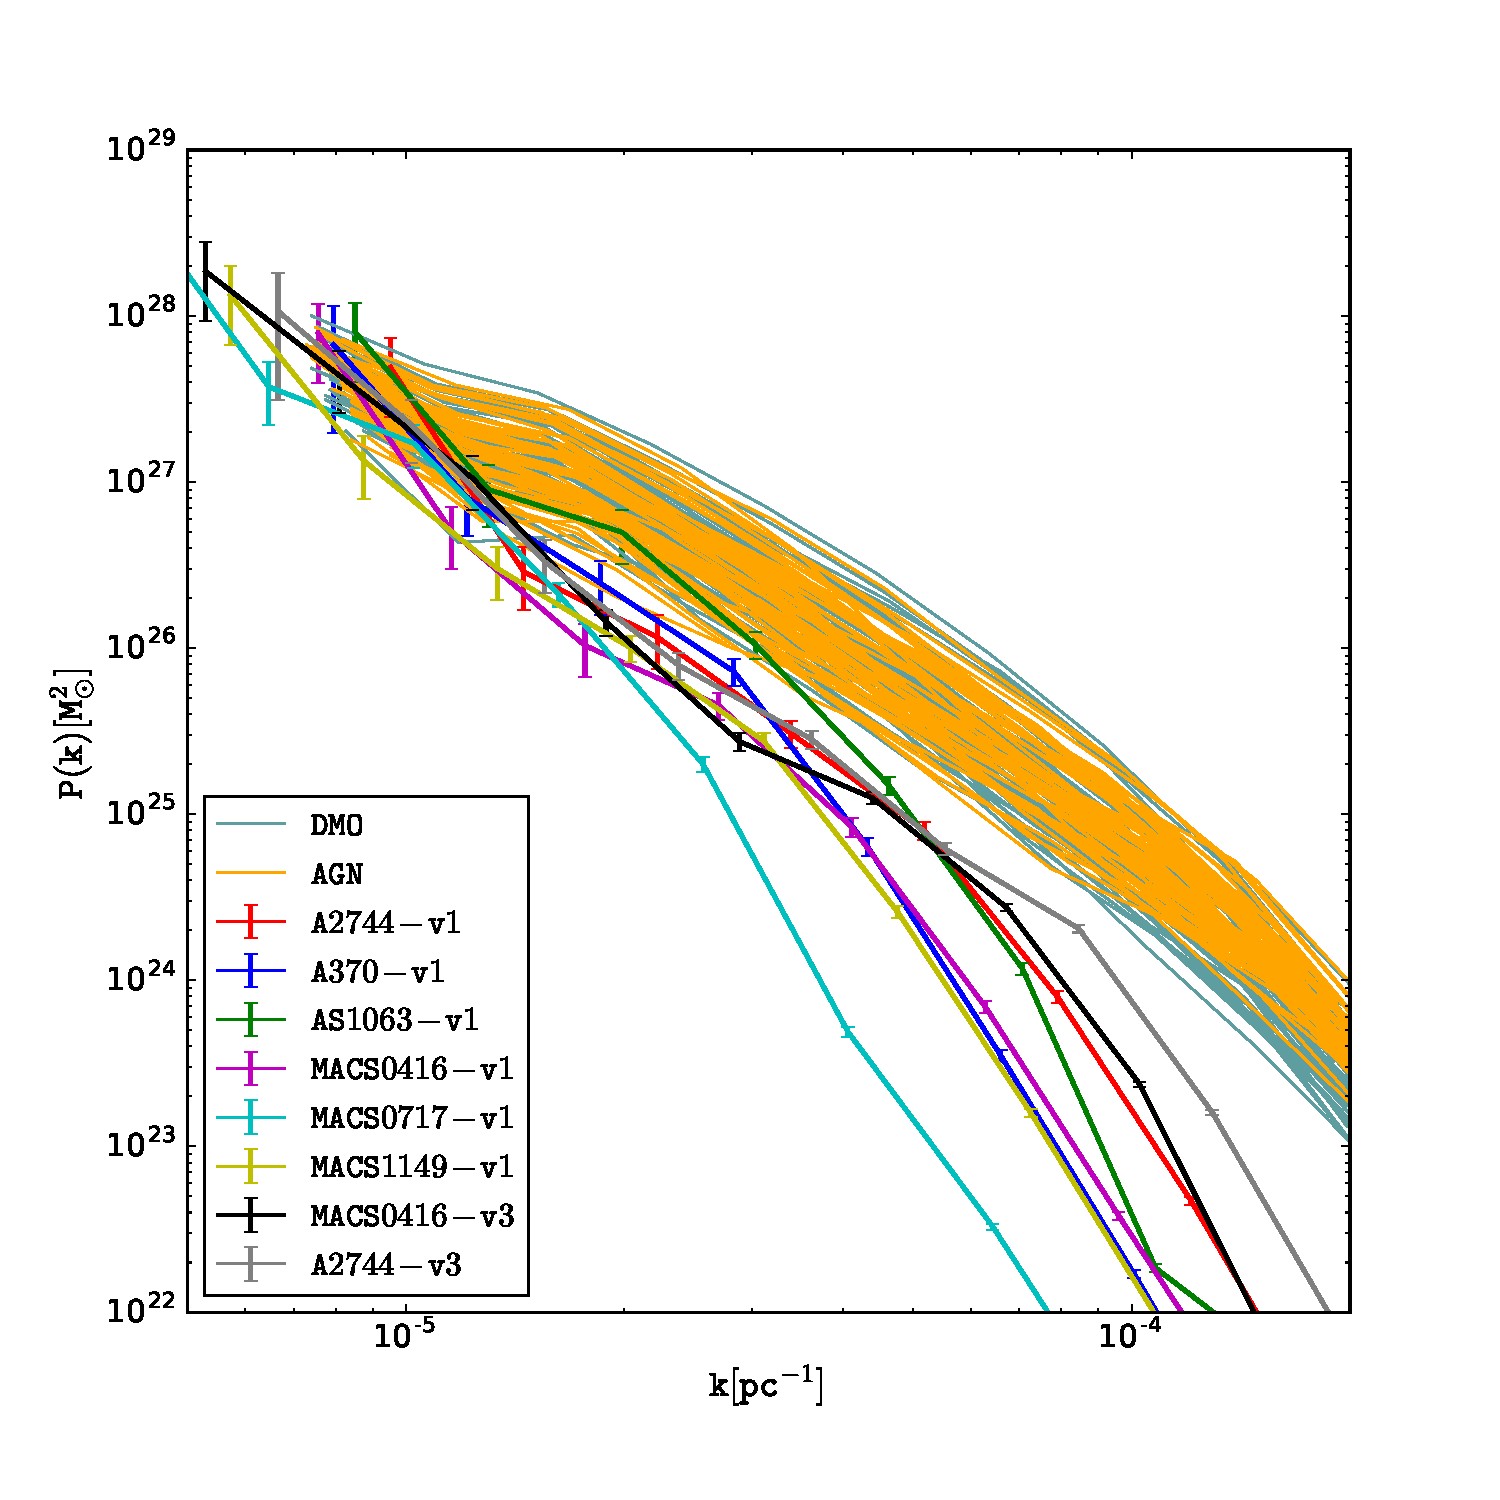
\includegraphics[width=0.48\textwidth]{figures/p5-figures/pk_pkofavgmap.pdf}
  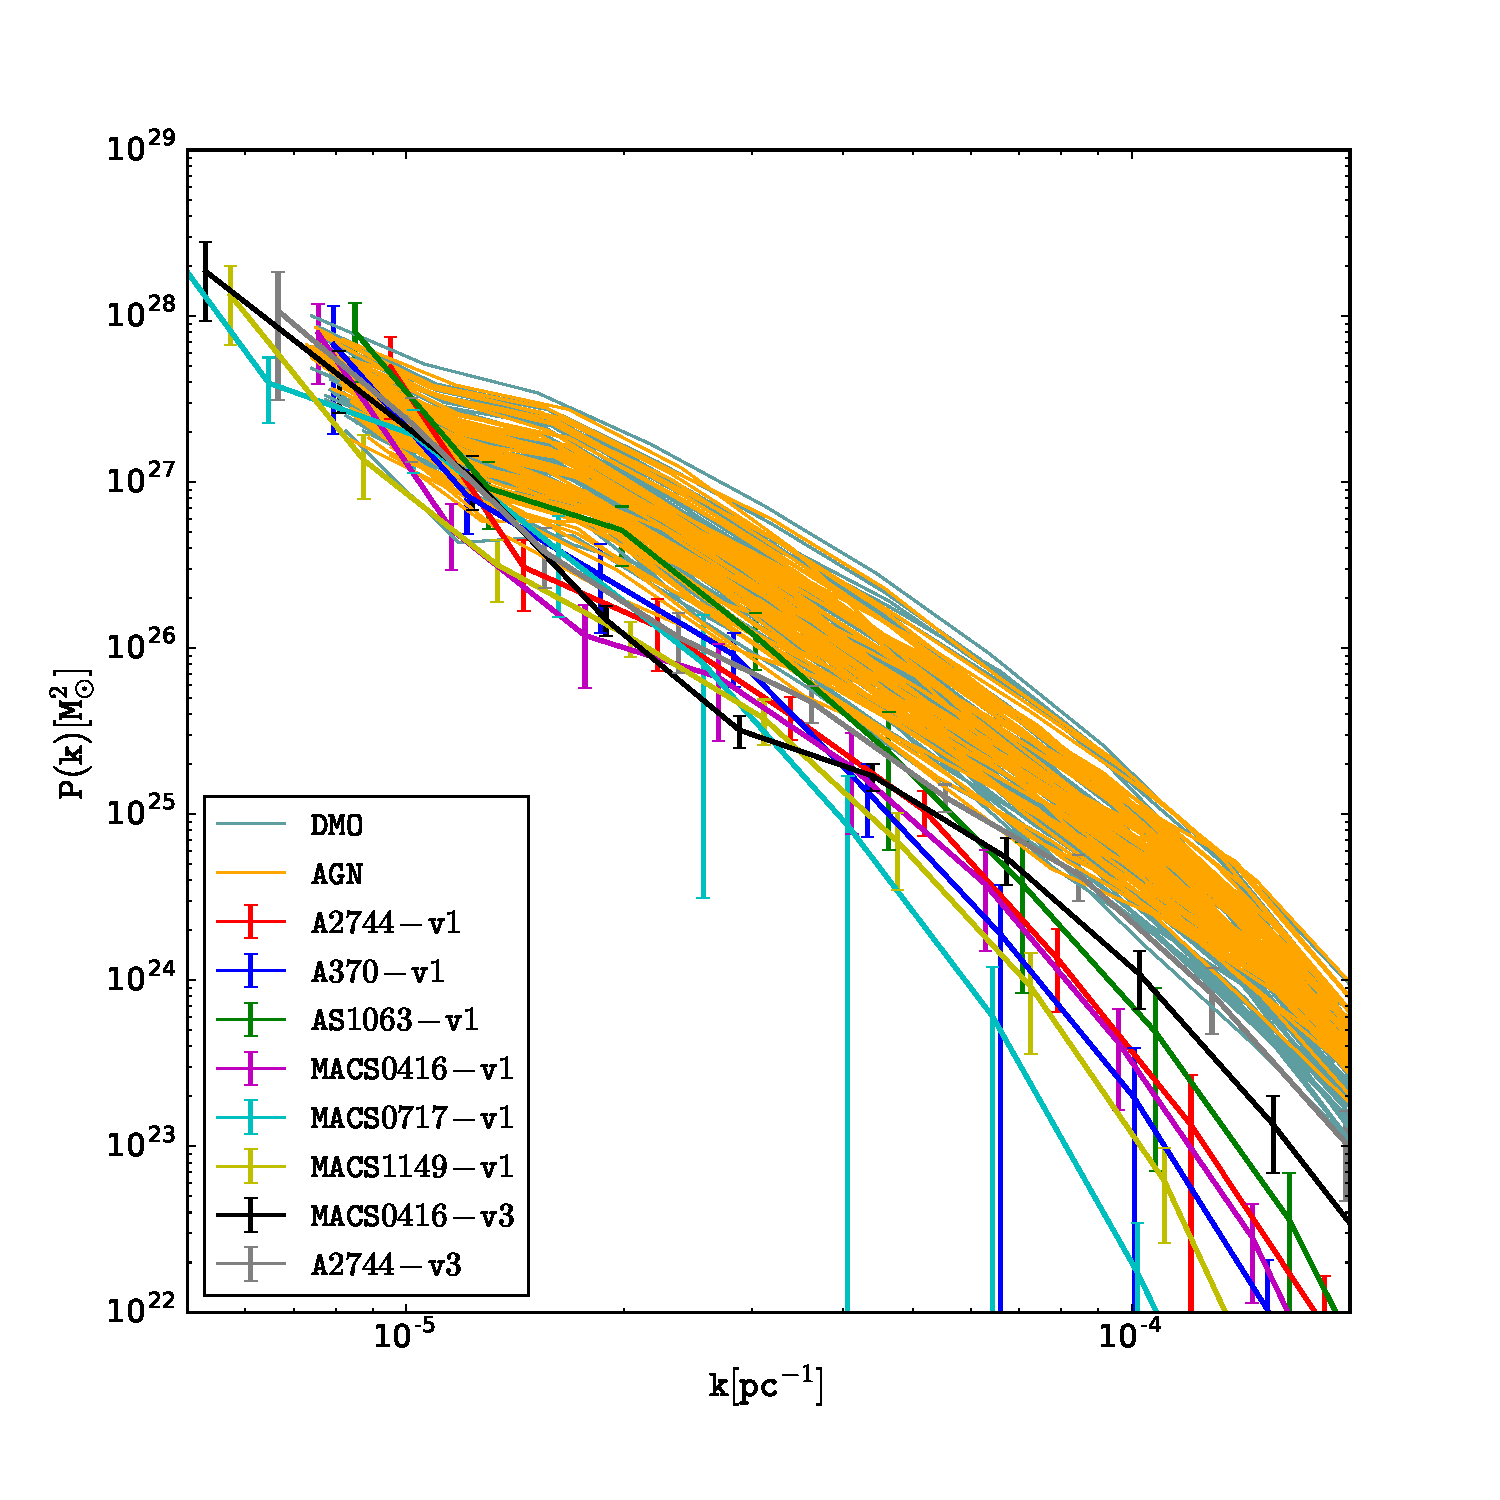
\includegraphics[width=0.48\textwidth]{figures/p5-figures/pk_avgofpk.pdf}
	\caption{All power spectra: clusters in thick solid lines and
	simulations in thin solid lines.
  Left: showing power spectra calculated for the average mass map of each
  cluster. The error bars are the scatter in different modes at a given $k$
  (or the sample variance).
  Right: each power spectrum is the average of 30 (40 in case of $\mathtt{v3}$) different power
  spectra calculated for each mass map in the ensemble for the respective
  cluster.
  The error bars are the standard deviation of the power spectra,
  including contributions from sample variance, as well as the scatter between different
	reconstructions of the same cluster.}
	\label{p5:fig:pkall}
\end{figure}


\begin{figure}
	\centering
	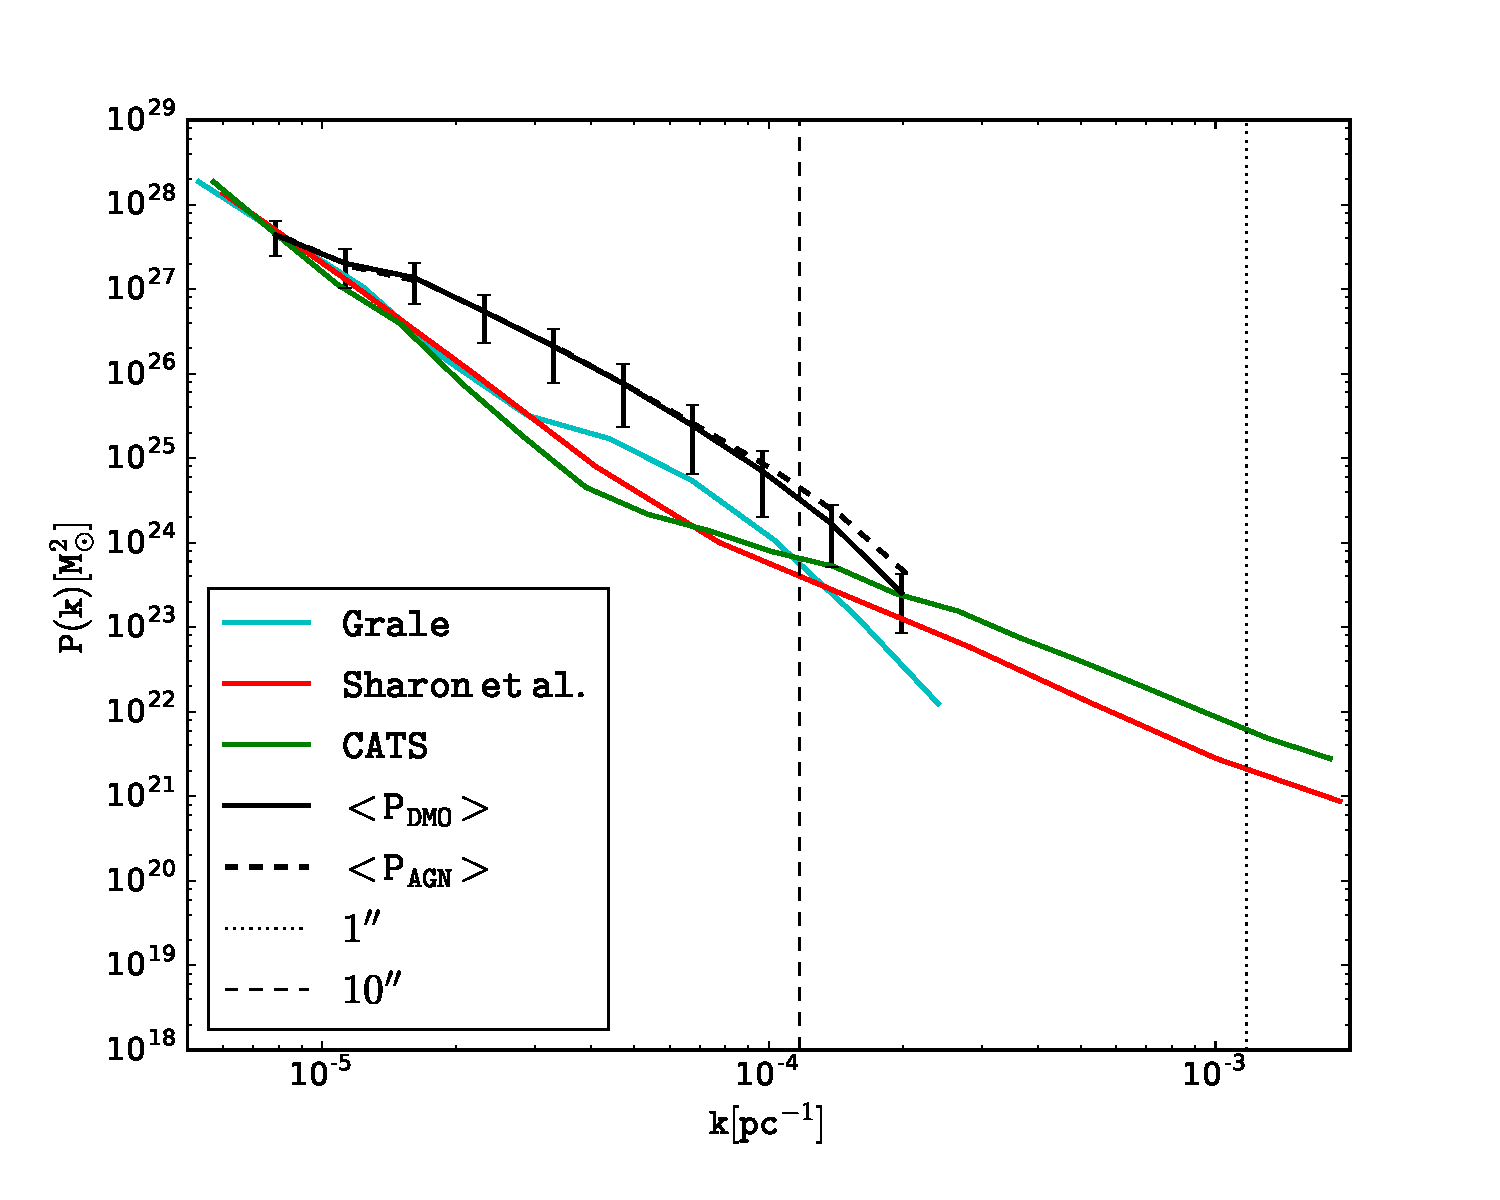
\includegraphics[width=0.48\textwidth]{figures/p5-figures/comparePk_grale_lenstool_v3.pdf}
	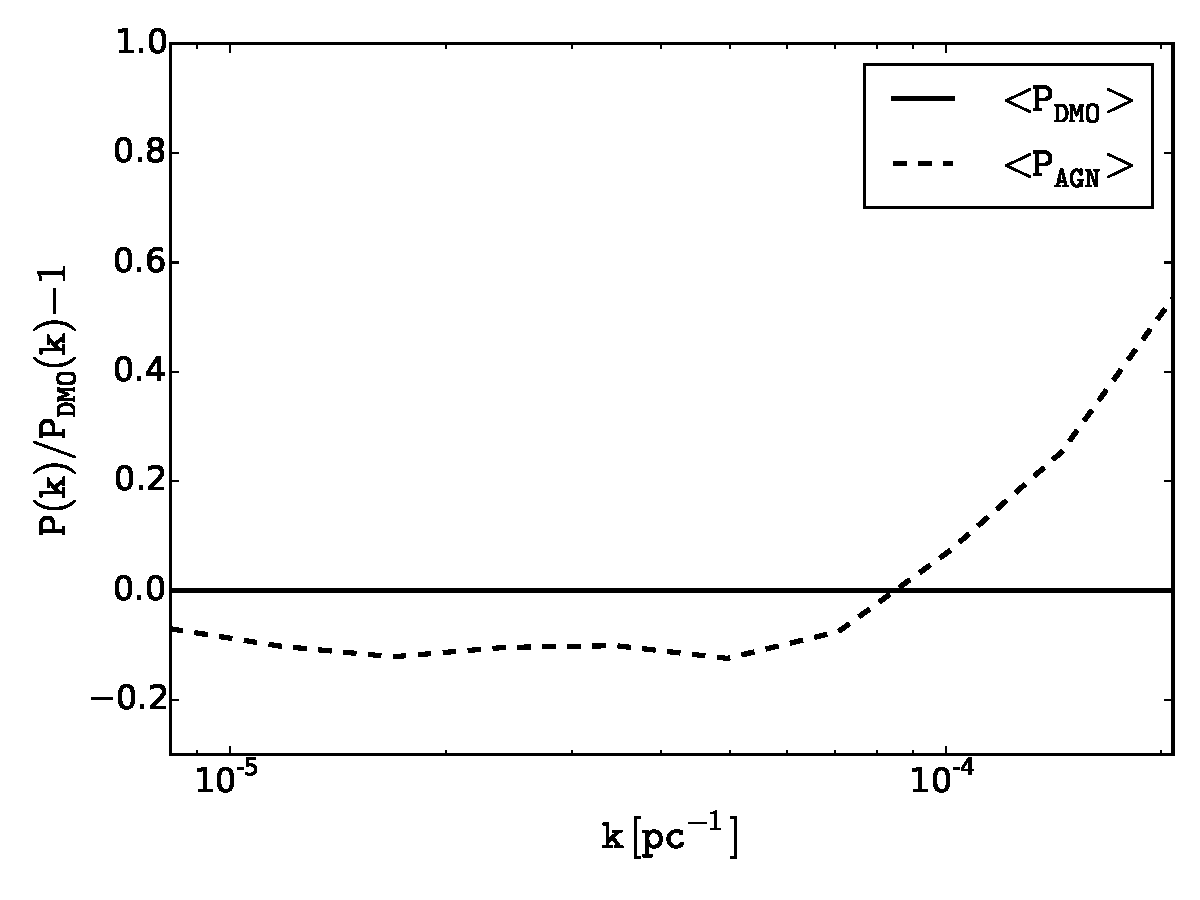
\includegraphics[width=0.48\textwidth]{figures/p5-figures/pk_simulations_relative.pdf}
	\caption{Left: comparing the mean power spectrum for dark-matter only simulations (DMO),
	baryonic simulation (AGN) and different reconstructions using GRALE and LENSTOOL for MACS0416-v3
	(using HFF data only). The vertical lines show the 10 and 1 arc second scales at the cluster's redshift
	$z=0.396$. Right: the relative difference between the
	mean power spectra of DMO and AGN simulations.}
	\label{p5:fig:pk:compare}
\end{figure}


\begin{figure}
	\centering
	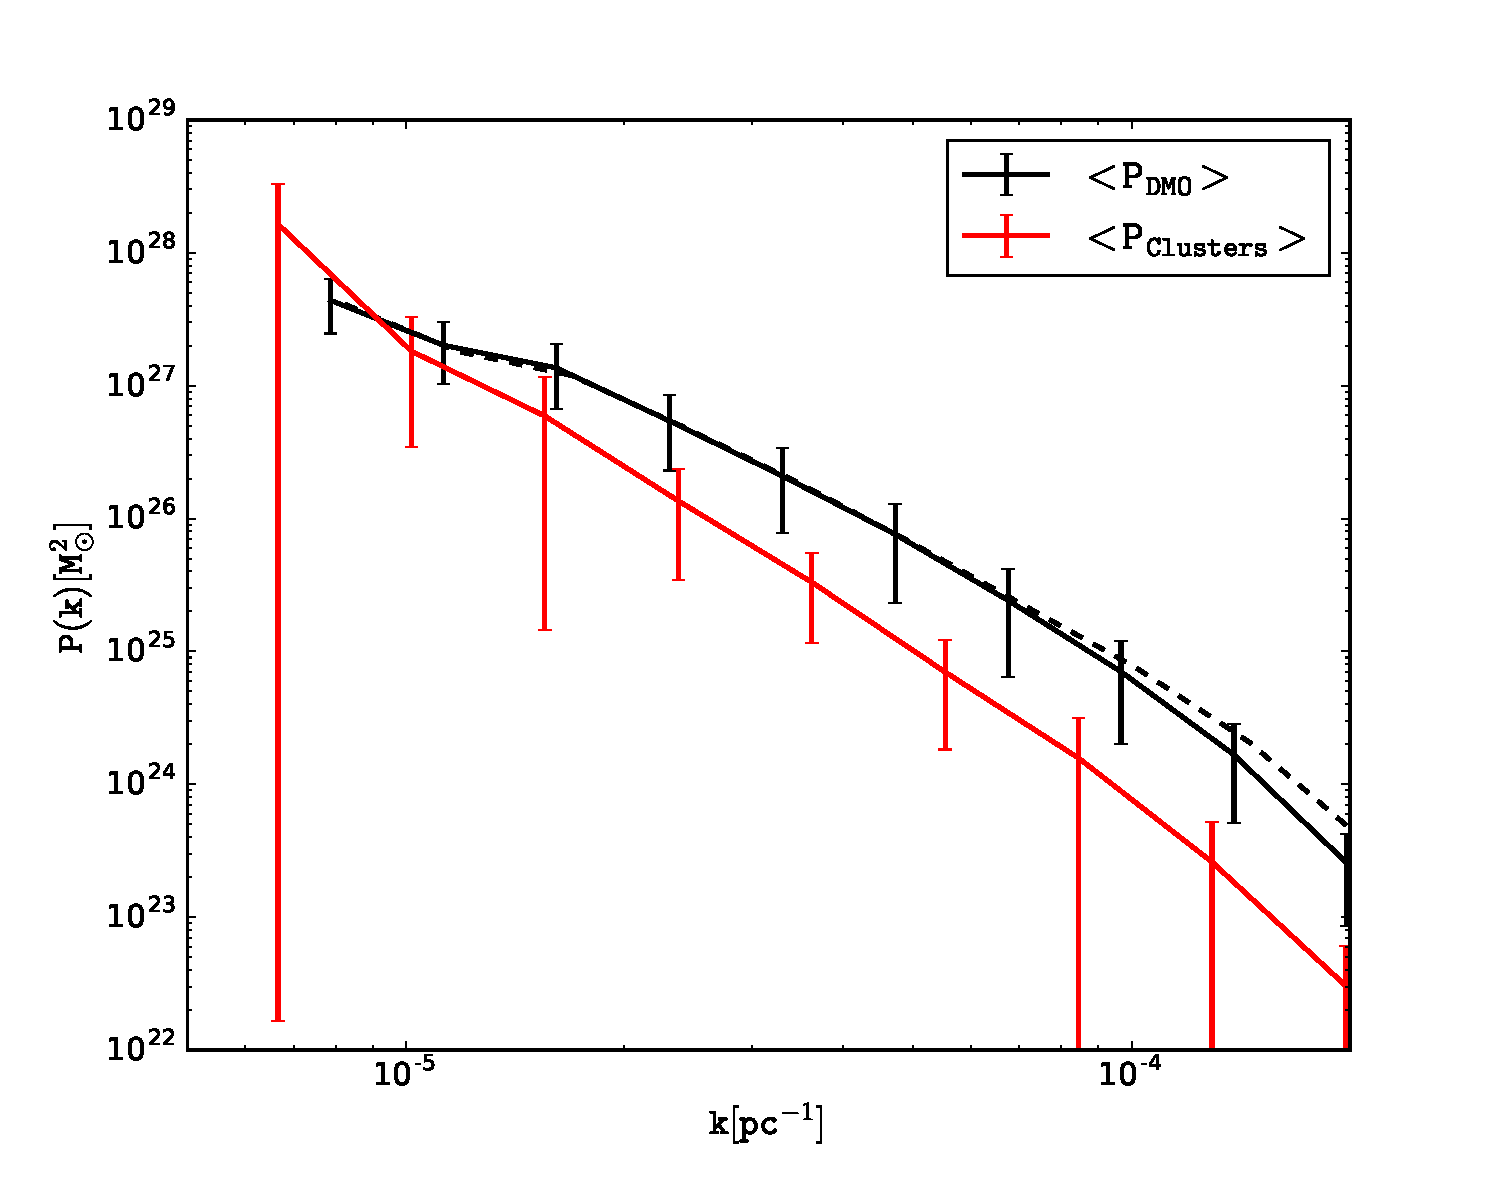
\includegraphics[width=0.8\textwidth]{figures/p5-figures/pkavgClustersSims.pdf}
	\caption{Comparing average power spectrum of HFF clusters to
				that of the simulated clusters.}
	\label{p5:fig:pk:sim}
\end{figure}



\subsection{Comparing HFF clusters}


We can now compare the clustering properties of HFF clusters
using the lensing power spectrum $P_{\rm M}(k)$ .
The reconstructed mass distributions of the HFF clusters are morphologically different but
show similar statistical structures which is very much evident from comparing the respective
power spectra. Figure \ref{p5:fig:pkall} shows all the power spectra for HFF clusters in
thick lines along with their sample variance, which represents scatter across
all available modes for a given $k$.

Let us first consider two reconstructions for MACS0416, using pre-HFF and HFF data. Both
mass maps are very similar at large scales but differ in detail at small scales. The
same effect can be noticed in the power spectrum (see figure \ref{p5:fig:pkall}): up to
$k \sim 3 \times 10^{-5} \rm{pc}^{-1}$ both look nearly the same, but at smaller scales
the mass map reconstructed with pre-HFF data starts to lose power. This is a
consequence of the fact that HFF data has over two times as many lensed images as pre-HFF
data (see table \ref{p5:tbl:HFF}), allowing for higher resolution in the reconstructed mass maps.
This leads to a higher power at small scales, where the difference in the two power spectra
is almost an order of magnitude. A similar trend can be seen in the two versions
of Abell 2744. 

Power spectra for Abell 370 and MACS1149 look very similar to each other. If we look at the corresponding mass maps, both show two dominant peaks with similar width, shallow as compared to the surroundings with similar smoothing.
Similar arguments can be made for Abell 2744 and MACS0416-II clusters.
The clusters show similar power at small scales which is expected from the very steep mass peaks in the two clusters.

It is important to note that the smallest scale (largest $k$) to be trusted depends on the density
of images. For example, MACS0416-v3 has 4 times more images than MACS0717, (assuming
roughly the same area for both in terms of arcsec$^2$), so the typical linear image
spacing is 2 times larger in MACS0717, leading to poorer mass
resolution. And, in fact,
looking at figure \ref{p5:fig:pkall}, the $k$ value where $P_{\rm M}(k)$  of MACS0717 begins to drop
($k\sim 2\times 10^{-5} {\rm pc}^{-1}$) is about a
factor of $\sim 2$ smaller compared to that of MACS0416
($k\sim 4\times 10^{-5} {\rm pc}^{-1}$).

There is also a tendency for low redshift clusters to have higher power at
small scales. Thus, Abell 2744 reconstructed with 41 images has larger power
than MACS0416-v1 (40 images) at small scales.
Similarly, MACS1149 has less power at small scales than A370 and AS1063, again with similar numbers of lensed images.
This is also intuitive as low redshift clusters have had more time to
build small-scale substructures.
Therefore, the power at small scales may be indicative of the age of the cluster.
% Therefore, by looking at the power at small scales with similar lensing data, one can
% get an idea about the respective merging stage of the clusters.

%------------------------------------------------
\subsection{\texorpdfstring{$\Lambda$CDM}{Lambda-CDM} simulation clusters}

We used 22 clusters of galaxies from dark-matter only (DMO) simulations and
an additional 22 from hydrodynamical simulations which include AGN feedback,
in the mass range  1--3$\times 10^{14} M_{\odot}$ from \cite{2014MNRAS.440.2290M}
using RAMSES \citep{2002A&A...385..337T}.
The mass range is chosen to be comparable to that of the HFF clusters but the
simulated clusters are all at redshift zero. We then projected
them along the three axes, for a total of 66 projected clusters in each case.
Projection does introduce some correlation in the sample, but we assume
such correlations in the sample, but we neglect this effect.
In contrast to HFF clusters, the simulation clusters are virialised but a few show more than one core.
The measured power spectra are shown as thin lines in figure \ref{p5:fig:pkall}.

We also measured the mean power spectrum in each case, DMO and AGN, which is shown in black
in the left panel of figure \ref{p5:fig:pk:compare}.
The error bars show the standard deviation of $P_{\rm M}(k)$, including contributions from
scatter in different modes at a given $k$ as well as the scatter between different clusters.
In the right panel of figure \ref{p5:fig:pk:compare}, we show
the relative difference between the mean power in DMO and AGN simulated clusters.
Comparing the mean power spectra of DMO and AGN, the latter shows a deficit in power
at large scales and a boost at smallest scales. The deficit is nearly $10\%$.
The AGN clusters have the influence of an AGN at the centre that drives the gas
outside the cluster with its feedback process. Losing this mass results in the
deficit of power at those scales. However, these AGN clusters contain a central
stellar component in the form of the brightest cluster galaxy (BCG),
which increases the mass at the very centre of the
cluster resulting in a boost in the power at smallest scales.
The trend is systematically consistent with previous findings.


\subsection{Comparison between HFF clusters and
  \texorpdfstring{$\Lambda$CDM}{Lambda-CDM} simulation clusters}

In figure \ref{p5:fig:pkall}, we show $P_{\rm M}(k)$ for all six HFF clusters as
well as both DMO and AGN for all the simulated clusters.
The lensing clusters systematically show less power at small scales
compared to the simulated ones.
We discuss the possible reasons for this in
section \ref{p5:sec:discussion}.


\subsection{Comparison with LTM models}


In the left panel of figure \ref{p5:fig:pk:compare}, we compare the power spectrum measured
from the mass maps reconstructed using GRALE to that made using other methods:
Sharon et al and the CATS group.\footnote{\tt https://archive.stsci.edu/prepds/frontier/lensmodels/}
Both use the LTM method LENSTOOL of \cite{2007NJPh....9..447J} as the reconstruction technique.
Both of these reconstructions show much larger
power at small scales compared to the GRALE reconstruction. This is the result of the fact that LENSTOOL uses
information from the individual cluster galaxies of the lens, and
hence has much steeper density gradients at small scales which results in
larger power. This effect is also seen in the galaxy-mass correlation function of
MACS0416 which shows a sharp peak at zero separation \citep{2015arXiv150708960S}.
The power spectrum of parametrically reconstructed clusters is a mixture
of priors and lensing information, and when the number of images is small, priors
are the dominant contribution.
In contrast, free-form methods like GRALE base the mass
distribution on the lensed images alone, without relying on visible galaxies.


%=================================================================================

\section{Conclusions and Discussions}\label{p5:sec:discussion}

In this article, we present free-form mass models of six Hubble Frontier Field
clusters using strong gravitational lensing pre-HFF data.
We also studied two of the six clusters, MACS0416 and Abell 2744, using both pre-HFF
and HFF data (with many more lensed images).
For each cluster, a total of 30 mass maps (40 for $\mathtt{v3}$ versions) are made
using a non-parametric lens inversion technique called GRALE, and the
average mass map is presented. All the mass
maps show elongation, multiple cores and many substructures in the mass
distribution implying a recent major merger. The lensing data from
recent HST-HFF observations is rich in lensing images allowing a very
precise identification of substructures to be done with greater
confidence. These mass maps can be used to study various aspects
of the structure formation and merging stages of large collapsed clusters
of galaxies.

We measured the power spectra of these sky-projected mass maps (30 for each cluster),
and presented both average power spectra, as well as the power spectra of the
average mass map for each cluster (figure \ref{p5:fig:pkall}). The error
estimates of the power spectra are either given as the scatter in different modes
at a given $k$, also known as sample variance, or a combination of the sample
variance and the standard deviation of the power spectra for the same cluster.
Power spectra give a statistical description of the clustering properties of the
mass distribution and encode information about the abundance of
substructures  and their contrast with the background.
There are tentative indications that low redshift clusters
have systematically higher power at small scales as compared
to high redshift clusters, presumably because low redshift
clusters are closer to their virial equilibrium than high redshift clusters.
We argue---and illustrate using pre-HFF and HFF maps of MACS0416---that using a
larger number of lensed images in a cluster leads to a better-constrained mass
distribution, and that the power spectrum
can be recovered up to much smaller scales putting stronger constraints
on our understanding of the substructures. On the other hand, parametric
methods that explicitly include cluster galaxies in the models have much larger power on small scales
even with fewer lensed images indicating that the mass maps are dominated
by the priors, especially at small scales.

We compared the power spectra of the HFF clusters with those from $\Lambda$CDM
dark-matter only and hydrodynamical simulations at redshift zero.
Figure \ref{p5:fig:pk:sim} summarizes our comparison between HFF clusters and
$\Lambda$CDM simulation clusters. We average the power spectra of the six HFF
clusters and compare them with the average power spectra of the simulated
clusters. The average power of the clusters is systematically steeper than
that of the simulated clusters and hence have less power at small
scales. This may be due to one or more of the following reasons:

\begin{itemize}
    \item The redshift of the HFF clusters are higher than the simulated clusters.
    We are comparing non-virialised HFF clusters with the virialised
    halos of the simulations. At later times, the mass distribution
    becomes more and more clumpy and the substructures pull
    more mass from the background,
    which results in a higher power at small scales. Therefore, it
    is possible that the lensing clusters in the local Universe may
    show similar power as the simulated clusters
    at redshift zero. Conversely, this can be checked by comparing
    the power spectrum of HFF clusters with that of simulated clusters of similar masses
    in the redshift range 0.3--0.5.

    Another effect of the redshift difference is that the angular resolution is lower for the higher redshift clusters. However, this effect is roughly 20$\%$, too small to account for the observed differences in the power spectrum.

    \item A second possible reason relates to the data and method we are
    using to reconstruct the clusters. A larger number of lensed images gives
    additional constraints on the mass distribution, and this increased resolution leads to a boost
    in the power spectrum. This can be seen in figure \ref{p5:fig:pkall}  where we show the power
    spectrum of MACS0416 using both pre-HFF and HFF data: HFF data shows
    larger power at small scales as compared to pre-HFF data.

    Figure \ref{p5:fig:pk:compare} shows that the power at small scales
    also depends on the assumption of the reconstruction method.
    It is possible that GRALE does not have enough resolution  and hence loses
    power at smallest scales. On the other hand, LENSTOOL maps seem to have
    much more power than expected at those scales and are possibly dominated by priors.

    \item Finally there is the possibility that the simulations are lacking
    some physics that needs to be taken into account in order to simulate
    realistic halos.
\end{itemize}

The second item above can be tested through a more extended pipeline, in which clusters are generated from
state-of-the-art simulations, lensing data are generated from them, and then analysed by independent groups
using different techniques.  Such tests are currently in progress.
%\footnote{\tt{http://pico.bo.astro.it/~massimo/Public/FF}}
% Hera \footnote{\tt{http://pico.bo.astro.it/~massimo/Public/FF/hera.html}}.
% These two clusters (and few more) are generated by the HFF consortium
% in order to compare the different mass mapping techniques. Both of them
% are rich in lensing data similar to the real HFF clusters with known
% mass distribution.
It will be interesting to measure the power
spectrum of the original mass distribution and the reconstructed one
using different lens inversion methods. %like GRALE, LENSTOOL etc.
The current analysis expects that the power spectrum based on GRALE maps
will match the true power spectrum at large scales and ultimately
lose power depending on the density of lensed images, whereas
LTM-based methods may continue having larger power even when the true power
drops. We leave this analysis for future work.

Independent of lensing, it will also be interesting to study the evolution of the power spectrum
as a probe of sub-structures and the merging history of large collapsed objects in simulations.
For example, a cosmological simulation can be set up with a volume large enough to produce
20--50 clusters of galaxies,  in a narrow mass range.  The power spectra can be calculated
for all the clusters in the mass range at different redshifts, and the evolution of the average
power spectrum can be studied. This will give us insight into the evolution of clustering
properties in a merging system. We leave this analysis to future work as well.


%=================================================================================



%=================================================================================

\section{Acknowledgement}

We would like to thank Davide Martizzi for providing the projected mass maps of the simulated clusters. 
IM would also like to thank Aurel Schneider for
useful discussions about the topic.

LLRW is grateful to the Minnesota Supercomputing Institute for their computational
resources and support.

We are grateful to the numbers of the HFF Map Maker teams, and especially to Dan
Coe, Johan Richard and Anton Koekemoer, who made their image identifications and
redshifts available to us, in some cases prior to publications for the v1 maps. Some
redshifts used were spectroscopic, some photometric and some were predicted by the
lens models. The relevant papers from which image information was taken are cited in
the text.
For v3 models, we are grateful to all those who contributed to the data used here:
members of the CATS team (including Mathilde Jauzac, Johan Richard, Jean-Paul
Kneib), GLAFIC team, Benjamin Clement, Adi Zitrin, Irene Sendra, Claudio Grillo,
Daniel Lam, Jose Diego, Xin Wang, Marusa Bradac, Austin Hoag, Traci Johnson, Brian
Siana, Anahita Alavi, Gabe Brammer, Tomasso Treu, Ryota Kawamata, and especially Dan
Coe and Keren Sharon.
  

IM is supported by Fermi Research Alliance, LLC under Contract No. De-AC02-07CH11359 with the United States Department of Energy.

%=================================================================================

\chapter{Conclusions}
\label{chap:conclusions}

In this PhD dissertation, I (along with other collaborators on different projects) tried
to build a better understanding of the distribution of 
matter in the Universe and its clustering properties, which I studied
in two very different regimes: gravitationally bound systems like 
cluster of galaxies, and the large scale structure of the Universe. 
While working on various projects on this topic, I successfully
completed five scientific publications:

\begin{itemize}
\item The very first project is a mass modelling problem in strong lensing cluster
  \cite{2014MNRAS.439.2651M}. Here we
  used a publicly available code GRALE, modified it for an optimum solution and resolution,
  to put tight constraints on the mass distribution of few lensing clusters. By studying
  the mass and light distribution of these clusters, we imply that it is possible 
  that the dark-matter has a finite self-interaction cross section and shows
  important signatures in the central parts of clusters. 

\item In a similar project, we show that the time delay information is very useful in 
  order to put additional constraints on the central region of the clusters which can't 
  be resolved directly, especially when the steepness degeneracy is broken by the 
  presence of background sources at different redshift \cite{2015PASJ...67...21M}.

\item We also presented a (semi) analytic model for the matter power spectrum, which is
  computationally inexpensive and computes the power spectrum to a percent level 
  accuracy up to k $\sim$ 1 $h^{-1}\mathrm{Mpc}$ \cite{2014MNRAS.445.3382M}. 
  The motivation of this model is the halo model
  and we also derived a simple form of the covariance matrix. We proposed a way to 
  marginalise over baryonic effects. 

\item In another project, we used the halo model in order to directly
  model the effects of baryons on the matter power spectrum and to the extension on the
  weak lensing shear power spectrum \cite{2014arXiv1410.6826M}. 
  The effects are small at comparatively large
  scales but as the next generation surveys are expected to measure these quantities 
  to very small scales, the baryonic effects are important to take into account. If not, 
  it will add biases to the cosmological parameters up to 10 sigma. 

\item Finally, we produced free-form mass models for six Hubble Frontier Field clusters.
  Their mass distribution shows elongation, multiple-cores, and many sub-structures
  indicating a recent major merger. We measured the power spectrum of the mass 
  distribution to quantify the sub-structures, and compared them to the simulated
  clusters.
\end{itemize}

\section{A Unified Picture}

If we try to draw a bigger picture from all the projects above, 
it states that it is very important to model baryonic physics 
in order to understand the clustering processes,
galaxy formation, and to do cosmology with future generation surveys. 

Gravitational lensing is one ideal tool to do accomplish this. Strong lensing
is very useful in studying the individual systems. 
Weak lensing shear measurements
on larger area in the sky is the most promising tool to do cosmology under
control systematics. One of the biggest source of systematics is again the 
baryonic effects at small scales, and there are various ways to handle them. But
they can't be ignored. Precision cosmology and detailed information about the 
individual systems is needed in order to gain full understanding of the 
galaxy formation processes and evolution of the Universe. 

\clearpage

\cleardoublepage
\backmatter
\KOMAoptions{bibliography=totoc}
\renewcommand{\bibname}{Bibliography}
\bibliographystyle{mn2e}
\bibliography{bibliography}

\end{document}
